%% LaTeX2e class for student theses
%% thesis.tex
%% 
%% Karlsruhe Institute of Technology
%% Institute for Program Structures and Data Organization
%% Chair for Software Design and Quality (SDQ)
%%
%% Dr.-Ing. Erik Burger
%% burger@kit.edu
%%
%% See https://sdq.kastel.kit.edu/wiki/Dokumentvorlagen
%%
%% Version 1.4, 2023-06-19

%% Available page modes: oneside, twoside
%% Available languages: english, ngerman
%% Available modes: draft, final (see README)
\documentclass[twoside, english, final]{sdqthesis}

%% ---------------------------------
%% | Information about the thesis  |
%% ---------------------------------

%% Name of the author
\author{Marco Schneider}

%% Title (and possibly subtitle) of the thesis
\title{HubLink: Leveraging Language Models for Enhanced Scholarly Information Retrieval on Research Knowledge Graphs}

%% Type of the thesis 
\thesistype{Master's Thesis}

%% Change the institute here, ``KASTEL'' is default
% \myinstitute{Institute for \dots}

%% You can put a logo in the ``logos'' directory and include it here
%% instead of the SDQ logo
% \grouplogo{myfile}
%% Alternatively, you can disable the group logo
% \nogrouplogo

%% The reviewers are the professors that grade your thesis
\reviewerone{Prof. Dr. Ralf H. Reussner }
\reviewertwo{Prof. Dr.-Ing. Anne Koziolek }

%% The advisors are PhDs or Postdocs
\advisorone{Dipl.-Inform. Angelika Kaplan }
%% The second advisor can be omitted
\advisortwo{Dr.-Ing. Jan Keim}

%% Please enter the start end end time of your thesis
\editingtime{30. November 2024}{30. May 2025}

\settitle

%% --------------------------------
%% | Bibliography                 |
%% --------------------------------

%% Use biber instead of BibTeX, see README
\usepackage[citestyle=numeric,style=numeric,backend=biber,sorting=none]{biblatex}
\addbibresource{references.bib}


%% ----------------
%% |   Acronyms   |
%% ----------------
\newacronym{ann}{ANN}{Approximate Nearest Neighbor}
\newacronym{enn}{ENN}{Exact Nearest Neighbor}
\newacronym{kg}{KG}{Knowledge Graph}
\newacronym{kge}{KGE}{Knowledge Graph Embedding}
\newacronym{kb}{KB}{Knowledge Base}
\newacronym{llm}{LLM}{Large Language Model}
\newacronym{lm}{LM}{Language Model}
\newacronym{tog}{ToG}{Think-on-Graph}
\newacronym{kbqa}{KBQA}{Question Answering over Knowledge Bases}
\newacronym{kgqa}{KGQA}{Question Answering over Knowledge Graphs}
\newacronym{qa}{QA}{Question Answering}
\newacronym{kglmqa}{KGLM-QA}{Knowledge Graph Language Model-Question Answering}
\newacronym{sqa}{SQA}{Scholarly Question Answering}
\newacronym{orkg}{ORKG}{Open Research Knowledge Graph}
\newacronym{rkg}{RKG}{Research Knowledge Graph}
\newacronym{swa}{SWA}{Software Architecture}
\newacronym{rag}{RAG}{Retrieval-Augmented Generation}
\newacronym{tgqa}{TGQA}{Template Generated Question Answering}
\newacronym{fcqa}{FCQA}{Final Curated Question Answering}
\newacronym{ap}{AP}{Asking Point}
\newacronym{eat}{EAT}{Expected Answer Type}
\newacronym{amt}{AMT}{Amazon Mechanical Turk}
\newacronym{se}{SE}{Software Engineering}
\newacronym{dsr}{DSR}{Design Science Research}
\newacronym{karagen}{KARAGEN}{Knowledge Augmented Retrieval and Generation ENgine}
\newacronym{rdf}{RDF}{Resource Description Framework}
\newacronym{iri}{IRI}{Internationalized Resource Identifier}
\newacronym{rgar}{RGAR}{Retrieval, Generation, and Additional Requirement}
\newacronym{gqm}{GQM}{Goal Question Metric}
\newacronym{gnn}{GNN}{Graph Neural Network}
\newacronym{ofat}{OFAT}{One-Factor-at-a-Time}
\newacronym{ecsa}{ECSA}{European Conference on Software Architecture}
\newacronym{icsa}{ICSA}{International Conference on Software Architecture}
\newacronym{cli}{CLI}{Command Line Interface}
\newacronym{bert}{BERT}{Bidirectional Encoder Representations from Transformers}
\newacronym{api}{API}{Application Programming Interface}
\newacronym{ce}{CE}{Carbon Emissions}
\newacronym{ec}{EC}{Energy Consumption}

\newacronym{ir}{IR}{Information Retrieval}
\newacronym{is}{IS}{Information System}
\newacronym{sp}{SP}{Semantic Parsing}

\newacronym{cot}{COT}{Chain of Thought}
\newacronym{tot}{ToT}{Tree of Thought}
\newacronym{rar}{RaR}{Rephrase and Respond}
\newacronym{qald}{QALD}{Question Answering over Linked Data}

\newacronym{eo}{EO}{Evaluable Output}
\newacronym{gt}{GT}{Ground Truth}

\newacronym{tp}{TP}{True Positive}
\newacronym{tn}{TN}{True Negative}
\newacronym{fp}{FP}{False Positive}
\newacronym{fn}{FN}{False Negative}
\newacronym{doi}{DOI}{Digital Object Identifier}

\newacronym{mrr}{MRR}{Mean Reciprocal Rank}
\newacronym{map}{MAP}{Mean Average Precision}
\newacronym{rouge}{ROUGE}{Recall-Oriented Understudy for Gisting Evaluation}
\newacronym{bleu}{BLEU}{Bilingual Evaluation Understudy}

\newacronym{grag}{GraphRAG}{Graph Retrieval Augmented Generation}

\newacronym{difar}{DiFaR}{Direct Fact Retrieval}

% To make Chapter capitalized
\addto\extrasenglish{%
  \def\chapterautorefname{Chapter}%
}

%% ====================================
%% ====================================
%% ||                                ||
%% || Beginning of the main document ||
%% ||                                ||
%% ====================================
%% ====================================
\begin{document}

%% Set PDF metadata
\setpdf

%% Set the title
\maketitle

%% The Preamble begins here
\frontmatter

%% LaTeX2e class for student theses: Declaration of independent work
%% sections/declaration.tex
%% 
%% Karlsruhe Institute of Technology
%% Institute of Information Security and Dependability
%% Software Design and Quality (SDQ)
%%
%% Dr.-Ing. Erik Burger
%% burger@kit.edu
%%
%% Version 1.5, 2024-02-12

\thispagestyle{empty}
\null\vfill
\noindent\hbox to \textwidth{\hrulefill} 
%
% Gemäß Studien- und Prüfungsordnung Bachelor Informatik des KIT,
% § 14 (5) vom 10.05.2022
% 
\iflanguage{english}{I declare that I have developed and written the enclosed
thesis completely by myself. 
I have not used any other than the aids that I have mentioned. 
I have marked all parts of the thesis that I have included from 
referenced literature, either in their original wording or paraphrasing their
contents. 
I have followed the by-laws to implement scientific integrity at KIT.}%
{Ich versichere wahrheitsgemäß, die Arbeit selbstständig verfasst, alle benutzten 
Quellen und Hilfsmittel vollständig und genau angegeben und alles kenntlich gemacht 
zu haben, was aus Arbeiten anderer unverändert oder mit Abänderungen entnommen wurde 
sowie die Satzung des KIT zur Sicherung guter wissenschaftlicher Praxis in der 
jeweils gültigen Fassung beachtet zu haben. }
 
 
%% ---------------------------------------------
%% | Replace PLACE and DATE with actual values |
%% ---------------------------------------------
\textbf{Karlsruhe, 30.05.2025}
\vspace{1.5cm}
 
\dotfill\hspace*{8.0cm}\\
\hspace*{2cm}(\theauthor) 
\cleardoublepage

\setcounter{page}{1}
\pagenumbering{roman}

%% ----------------
%% |   Abstract   |
%% ----------------
 
%% For theses written in English, an abstract both in English
%% and German is mandatory.
%%
%% For theses written in German, a German abstract is sufficient.
%%
%% The text is included from the following files:
%% - sections/abstract

\includeabstract

%% ------------------------
%% |   Table of Contents  |
%% ------------------------
\tableofcontents

\listoffigures
\listoftables

\printglossaries

%% -----------------
%% |   Main part   |
%% -----------------



\mainmatter

\glsresetall    
\chapter{Introduction}
\label{ch:introduction}

% \glspl{llm} like GPT-4 \cite{openai_gpt-4_2024} and Flan-T5 \cite{chung_scaling_2022} sparked a revolution in the field of natural language processing tasks. These models are built on the transformer architecture \cite{vaswani_attention_nodate} and trained on extensive datasets scaled to billions of parameters, which leads to remarkable abilities in zero-shot learning, step-by-step reasoning, in-context learning, instruction following, human alignment, and tool manipulation \cite{yang_give_2024}. 

% Providing textual answers to user questions, relieve users of the cognitive effort of collecting the needed information from individual search results themselves.

% Question answering is a retrieval task more challenging than common search engine tasks because its purpose is to find an accurate and concise answer to a question rather than a relevant document. The difficulty is more acute in tasks such as story comprehension in which the target text is less likely to overlap with the text in the questions. For this reason, advanced natural language techniques rather than simple key term extraction are needed. \cite{Learning Question Classifiers by Xin Li}

% GraphRAG is still in its early stages \cite{peng_graph_2024}

% \section{Motivation}
% \label{sec:motivation}

% - Scholarly Literature Search is time-consuming and cognitively demanding, nowadays all research findings are communicated via digital scholarly articles, a practice often referred to as the document-centric approach \cite{jaradeh_open_2019-1,auer_towards_2018}
% - Research Knowledge Graphs can help to make research more efficient
% - But to query information from the graph is also demanding as the user is required to know the graph structure to traverse the graph to find related information 
% - Recent development in the literature unifies LLMs with Graphs to exploit the advantages from both: 
% -- LLM Advantages: General Knowledge, Language Processing, Generalizability
% -- Graph Advantages: Structural Knowledge, Accuracy, Deciseveness, Interpretability, Domain-specific Knowledge, Evolving Knowledge
% - Graph Retrieval Augmented Generation (GraphRAG) \cite{peng_graph_2024} has been established which utilizes LLMs to retrieve relevant knowledge from the graph given a natural language question
% - As shown by current approaches, adding a Graph to the Retrieval can improve the quality and reliability of answers generated by LLMs \cite{edge_local_2024, guo_lightrag_2024}
% - Most current graph retrieval approaches focus on general domains and it is unknown how they perform in the scholarly literature search task
% - However some research is starting on the scholarly domain \cite{jaradeh_question_2020,taffa_leveraging_2023,giglou_scholarly_2024}


% Need to add somewhere:
% - We developed a question taxonomy that with the goal: “The taxonomy is designed to classify the characteristics of questions posed to KGQA retrieval systems in the literature search domain, enabling the creation of diverse question sets that test a broad range of retrieval capabilities.”
% - We created HubLink, a new retrieval approach that leverages the structure of RKGs to improve the relevance and accuracy of retrieved contexts and be able to answer complex questions that are asked in the literature search.
% - We evaluated against baselines that are training free (as our approach) which means that they use pre-trained LLMs and do not require further fine-tuning or training of models. \cite{jiang_structgpt_2023}, \cite{sun_think--graph_2024}, \cite{wen_mindmap_2024}, \cite{sui_fidelis_2024}, \cite{baek_direct_2023}
% - Approaches like semantic parsing struggle because of: Semantic Parsing hat allerdings zwei bedeutende Herausforderungen wie von \textcite{gu_knowledge_2022} herausgestellt: \emph{Schema-Level Complexity} und \emph{Fact-Level Complexity}. Zunächst ist das Schema eines modernen \gls{kg} extrem reichhaltig was bedeutet, dass die Anzahl an Items eines Schemas mehrere tausend beinhalten kann. Beispielsweise hat der FREEBASE \gls{kg} über 8k an Schema items. 
% - Klar machen warum es sinnvoll ist das man Knowledge Graphen verwendet statt einfach direkt die Informationen zu embedden -> Auf Die Paper LightRag und MicrosoftGRAPH rag \cite{edge_local_2024, guo_lightrag_2024} verweisen die das zeigen. Also im Prinzip ist es in der Motivation schonmal wichtig klar zu machen warum der Ansatz gebraucht wird. Also das Sparql Generierung nicht aussreicht und das nur das Document Embedding auch nicht reicht

Today, almost all scholarly findings are communicated through digital scholarly articles, a practice often referred to as the document-centric approach \cite{jaradeh_open_2019-1,auer_towards_2018}. Although the transition from print to digital has significantly improved accessibility \cite{sompel_all_2009,bosman_scholarly_2017}, it still does not fully take advantage of modern digital technologies. In current research practice, each publication is treated as an isolated unit of knowledge, making it challenging to interlink related findings, methodologies, and underlying data. This isolation becomes especially problematic given the exponential growth of scientific literature \cite{bornmann_growth_2021}. Researchers must navigate an extensive body of text to identify relevant insights. This process is challenging due to the sheer volume of content and also the addition of inherent issues that plague text searches. For example, the lexical gap problem, in which misspellings, synonyms, abbreviations, ambiguous words, and the ignored word order hinder the effectiveness of searches \cite{li_unsupervised_2022}. Consequently, literature search becomes a time-consuming and cognitively taxing process, requiring careful crafting of search queries, manual sifting through countless documents, and painstaking synthesis of scattered evidence. 

Recently, \glspl{llm} have demonstrated powerful capabilities in understanding natural language, expressiveness, general knowledge, and generalization \cite{yang_give_2024}. In the context of \gls{qa}, integrating \glspl{llm} allows users to pose queries in natural language, with the system generating relevant answers. This is particularly interesting for scholarly literature search as it allows researchers to find answers to scientific resources by asking questions in natural language, effectively reducing manual effort. However, using the pre-trained internal knowledge of the \glspl{llm} is not sufficient because their answers may lack depth, be subject to hallucinations, and do not provide transparency regarding the underlying reasoning process \cite{yang_give_2024}. 

To mitigate these issues in the \gls{qa} setting, \gls{rag} has emerged, in which an external \gls{kb} is used to provide relevant context to the \gls{llm} to enhance the answer generation \cite{lewis_retrieval-augmented_2021}. In this framework, an indexing phase takes place where the collection of documents is split into text chunks, which are then converted into dense vector representations and stored in a vector store. At query time, the vector representation of the question is used to conduct a distance-based search in the vector space to find the most relevant text chunks. Although this approach can be applied to the scholarly literature search setting \cite{lu_dense_2024}, naive \gls{rag} encounters notable drawbacks. Retrieval can suffer from poor precision and recall, missing crucial context, or retrieving irrelevant information \cite{gao_retrieval-augmented_2024}. Furthermore, \glspl{llm} often struggle with noisy or misleading documents, fail to abstain from answering when relevant information is absent, perform poorly at integrating information across multiple sources, and are prone to accepting factual errors in the retrieved context \cite{chen_benchmarking_2023}.

An alternative to document-centric knowledge representation is to structure and interconnect representations of scholarly knowledge \cite{jaradeh_open_2019-1}. This can be achieved using \glspl{kg} where knowledge is curated from structured and unstructured sources \cite{verma_scholarly_2023}. Specifically for the academic domain, these graphs are referred to as \glspl{rkg} and offer a promising solution to structure and interlink scholarly information. With the aim of transforming scientific communication from document-centric to knowledge-centric \cite{auer_towards_2018}, \glspl{rkg} provide a structured and machine-readable representation of scholarly knowledge by taking into account the relationships between texts and the incorporation of structural information as additional knowledge \cite{peng_graph_2024}.

The unification of \glspl{llm} and \glspl{kg} is a relatively new research field that aims to utilize the advantages of both in various applications \cite{pan_unifying_2024}. One such application is \gls{kgqa}, where the integration of knowledge from a \gls{kg} to inform the \gls{llm} during inference is investigated \cite{banerjee_knowledge_2024,chakraborty_introduction_2021,chakraborty_introduction_2019,pan_unifying_2024,yani_better_2022,peng_graph_2024,jin_large_2024,feng_trends_2023,li_survey_2024,agrawal_can_2024,procko_graph_2024}. 
Although many \gls{kgqa} approaches have emerged, most of the approaches are focused on open-domain \gls{qa} and have not yet been tested in the scholarly field. Furthermore, approaches explicitly aimed at the scientific field focus primarily on \gls{sp} methods that automatically create structured queries from natural language queries using training examples \cite{banerjee_dblp-quad_2023, taffa_leveraging_2023, lehmann_large_2024, jiang_structure_2023, jaradeh_question_2020}. 

Despite being effective in controlled settings, \gls{sp} methods struggle to adapt to dynamically evolving \gls{kg} schemas, leading to poor performance when encountering previously unseen entities or relations. In addition, semantic parsing approaches face significant scalability challenges, including both schema-level and fact-level complexities \cite{gu_knowledge_2022}. These problems are exacerbated by the extensive schema richness of modern \glspl{kg}, which often encompasses thousands of schema items. Moreover, semantic parsing methods typically require manually curated training datasets, which are costly to produce and limit their applicability in real-world research environments, making the methods inconvenient to use. 

Consequently, we identify a research gap in applying alternative \gls{llm}-based strategies to the scholarly \gls{kgqa} task. Most alternative strategies are developed and evaluated on general-purpose graphs like Freebase or Wikidata \cite{peng_graph_2024}. However, these approaches cannot be easily adapted to the scholarly domain \cite{saikh_scienceqa_2022}. Moreover, current retrieval approaches often ignore the source diversity of retrieved information, potentially returning multiple pieces of information from the same publication, reducing the breadth of evidence needed for robust scholarly inquiries. Therefore, the scholarly domain remains underexplored within \gls{kgqa} research.

Motivated by these challenges, we argue that research on scholarly \gls{kgqa} should explore directions beyond semantic parsing to develop methods that do not require training or fine-tuning and can adapt to dynamically changing \gls{kg} schemas. Our thesis contributes a novel \gls{kgqa} retrieval approach that complies with the above-mentioned criteria. We rigorously evaluated the approach on a scholarly literature search task in a \gls{swa} setting against five state-of-the-art baseline \gls{kgqa} approaches on the \gls{orkg} to demonstrate its superiority in retrieval performance. We further contribute a new taxonomy for the classification of questions querying \gls{kgqa} systems for literature search. With these contributions, our aim is to advance research in the direction of \gls{kgqa} in the scholarly literature search domain.


% In summary, despite promising advances in \gls{grag} and \gls{kgqa}, the academic domain remains underexplored. Existing methods either depend on general purpose graphs that fail to capture the specific request of literature search or rely on semantic parsing methods that struggle with evolving and scaling \gls{kg} schemas. Therefore, more research is required to achieve a robust, scalable, and schema-agnostic retrieval approach tailored for scholarly \glspl{kgqa}.

% Although helpful, this document-centric approach still struggles with precision and recall in \gls{qa} tasks \cite{gao_retrieval-augmented_2024}.

% By encoding semantic and relational information, \glspl{rkg} facilitate sophisticated queries and structured retrieval that surpass traditional keyword-based methods. 

% Despite these advantages, effectively querying an \gls{rkg} remains challenging. Traditional methods such as manually crafting SPARQL queries require users to possess in-depth knowledge of the graph schema. Even with user-friendly interfaces like that of the \gls{orkg} \cite{jaradeh_open_2019}, navigating these graphs can be cumbersome, particularly for complex queries.


% into the \gls{rag} framework, forming what is now known as \gls{grag} \cite{peng_graph_2024, pan_unifying_2024}. \gls{grag} approaches leverage the structured, relational nature of \glspl{kg} to retrieve more relevant and interpretable contexts. A growing body of research demonstrates the effectiveness of these methods in various domains \cite{pan_unifying_2024,peng_graph_2024,jin_large_2024,feng_trends_2023,li_survey_2024,agrawal_can_2024,procko_graph_2024}.



% Furthermore, we observe that many current retrieval approaches require additional training or fine-tuning prior to the retrieval process. 
% This is a significant limitation, as it requires ground truth data, which is often unavailable. 
% We envision, that for useability in practice, a retrieval approach should be \enquote{plug-and-play}, meaning that it should not require any training or fine-tuning prior to the retrieval process. 
% As such, \emph{the approach should only require the \gls{rkg} and no additional ground truth data}. 


% Moreover, we identified that many current retrieval approaches are only considering the retrieval of single entities as oposed to complex natural language answers.

% Researchers are confronted with the task of navigating the immense growth of scientific literature \cite{bornmann_growth_2021}, which is made even more difficult as there is no dedicated database for scientific literature. As consequence, researchers have to use academic search engines to find relevant literature. 

% Traditional results from search engines include a list of links to information sources that may contain the answer to the question of the user. However, this approach requires cognitive effort from the user to collect the needed information from the individual search results. To relieve users of this effort, the design of result presentation from search engines has changed with the introduction of \glspl{llm} as illustrated in \autoref{fig:new_search_engine_results_page}. Instead of providing a list of links, the search engine now provides textual answers each linked to the source of the information \cite{gienapp_evaluating_2024}.

% \begin{figure}
%     \centering
%     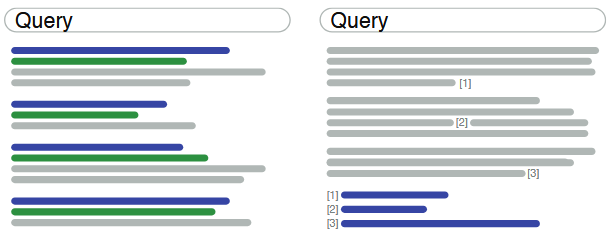
\includegraphics[width=1.0\linewidth]{figures/new_search_engine_results_page.png}
%     \caption{Change of results presentation in search engines \cite{gienapp_evaluating_2024}}
%     \label{fig:new_search_engine_results_page}
% \end{figure}

% The research community has proposed many QA systems, but to the best of our knowledge none focus on scholarly knowledge \cite{jaradeh_question_2020}

% TODO ADD Semantic Parsing Discussion:

% Semantic Parsing methods are early adopters for \gls{qa} on \glspl{kg}. These methods convert questions into a structural query such as SPARQL

% However, these methods heavily rely on the quality of generated queries. If the query is not executable, no answer will be generated. \cite{sui_fidelis_2024}
% Most important: Knowledge Base Question Answering: A Semantic Parsing Perspective
% Auch nochmal schauen warum Embeddingbasierte Ansätze Probleme hat
% Klar machen warum es sinnvoll ist das man Knowledge Graphen verwendet statt einfach direkt die Informationen zu embedden -> Die Paper LightRag und MicrosoftGRAPH rag verweisen die das zeigen. Also im Prinzip ist es in der Motivation schonmal wichtig klar zu machen warum der Ansatz gebraucht wird. Also das Sparql Generierung nicht aussreicht und das nur das Document Embedding auch nicht reicht

\section{Problem Statements}
\label{sec:problem_statements}

\gls{kgqa} approaches show promising results in the \gls{qa} setting. However, most approaches are applied to the general-purpose domain and are not tailored to scholarly content. Those approaches that target scholarly \gls{kgqa} often rely on \gls{sp} techniques that struggle with dynamically evolving schemas and often require training data. As a result, the potential of applying \gls{kgqa} to support effective scholarly search remains largely untapped, leading to our first problem statement:

\begin{enumerate}[label=\textbf{P\arabic*}, leftmargin=2.5em]
    \item \label{enum:p1} There is an underexplored potential in applying \gls{kgqa} in the scholarly domain to help researchers find relevant literature faster and more reliably. Initial approaches show promising results, but they struggle with evolving schemas and often require training data. This problem hinders the practical application of \gls{qa} systems on the scholarly literature search task in real-world scenarios. 
\end{enumerate}

The application of a \gls{kgqa} approach to an \gls{rkg} has the potential to help researchers in finding related literature faster and more reliably. This is made possible through the natural language capabilities of \glspl{llm} that allow researchers to ask for information of interest using natural language rather than having to manually search for it. 

To assess whether such a \gls{kgqa} system is capable of answering desirable questions for literature search, a taxonomy can help. Such a taxonomy classifies questions according to their complexity and the retrieval capabilities required to arrive at the answer. Although there are existing taxonomies, such as in DBLP-QuAD \cite{banerjee_dblp-quad_2023} and SciQA \cite{dubey_lc-quad_2019} for \gls{kgqa} or the works provided by \textcite{li_learning_2002} and \textcite{singhal_att_1999} for general \gls{qa}, they often propose divergent classification schemes. Without a synthesized and domain-relevant taxonomy, it is challenging to assess whether a given system can handle the full range of question types and retrieval complexities found in scholarly search tasks. Such a taxonomy can be helpful to guide the development of robust \gls{kgqa} datasets used for benchmarking and tailored to the needs of researchers, leading to our second problem statement:

\begin{enumerate}[label=\textbf{P\arabic*}, leftmargin=2.5em, start=2]
    \item \label{enum:p2} There is a lack of a taxonomy that allows the classification of the characteristics of questions posed to \gls{kgqa} retrieval systems in the scholarly literature search task. This hinders the creation of diverse question datasets to test the retrieval capabilities of \gls{kgqa} approaches on different \gls{rkg}. 
\end{enumerate}

Using such a taxonomy and applying it to the scholarly literature search task can help in the process of creating \gls{qa} datasets to reliably determine whether a retrieval approach is able to meet its challenges.

% The primary objective of this thesis is to design, implement, and evaluate a new training-free and schema-agnostic retrieval approach that takes advantage of the inherent structure of \glspl{rkg} to improve the quality and reliability of \gls{qa} systems for literature search tasks.

% Although HubLink is designed to be domain-agnostic, this work focuses on its application within the scholarly domain, using the \gls{orkg} as a representative \gls{rkg} for empirical evaluation.

% HubLink is built on the insight that \glspl{rkg} organize knowledge around publication nodes, forming natural \enquote{hubs} of semantically related information. By exploiting this structure and incorporating source diversity during retrieval, HubLink addresses key challenges in scholarly question answering particularly those involving multiple constraints and the need to aggregate evidence from various sources.


\section{Objective and Research Questions}

After discussing the potential benefits and importance of utilizing \gls{kgqa} to enhance the search of scholarly literature and addressing the issues with existing approaches (\textbf{P1}) together with the evaluation of \gls{kgqa} retrieval systems (\textbf{P2}), we establish the research objective of this thesis as follows:

\begin{tcolorbox}
    \textbf{Research Goal:} Design a training-free and schema-agnostic retrieval approach leveraging \glspl{rkg} and pre-trained \glspl{llm} that enhances the quality, transparency, and reliability of context retrieval in \gls{kgqa} systems specifically tailored to scholarly literature search tasks. Additionally, construct a taxonomy for classifying questions posed to \gls{kgqa} retrieval systems to support the assessment of capabilities and performance of such systems in the scholarly literature task.
\end{tcolorbox}

A new retrieval approach that does not rely on a \gls{kg} schema and is training-free would benefit the exploration of the potential that such systems can have in literature search tasks. This addresses the first problem, \textbf{P1}. Furthermore, a taxonomy for characterizing questions in \gls{kgqa} retrieval can help to guide the construction of \gls{kgqa} datasets used for benchmarking retrieval systems. This addresses the second problem, \textbf{P2}.

To achieve this goal, the thesis is guided by research questions. The first question concerns the design and technical foundation of the new \gls{kgqa} retrieval approach:

\begin{enumerate}[label=\textbf{RQ\arabic*}, leftmargin=2.5em]
    \label{enum:rq1}
    \item How can a schema-agnostic retrieval algorithm leveraging an \gls{rkg} and a pre-trained \gls{llm} be developed for the \gls{kgqa} setting to effectively integrate diverse scholarly sources, adapt to evolving schemas and account for the provenance of information during retrieval without relying on training data?
\end{enumerate}

This research question addresses the first problem (\hyperref[sec:problem_statements]{\textbf{P1}}) as it directly targets the limitations of current scholarly \gls{kgqa} approaches. By developing a schema-agnostic and training-free approach, it explores the potential of retrieval without relying on the schema of the \gls{rkg} and thus is scalable and dynamically adaptable. Furthermore, without the requirement of a training dataset, the approach becomes more conveniently applicable and thus more relevant to apply in a real-world use case. Moreover, accounting for the provenance of information during inference is a critical aspect of scholarly literature search, as it supports the generation of complete, transparent, and balanced results. Provenance awareness helps prevent over-reliance on a single source and encourages the integration of diverse perspectives, ensuring that results capture complementary aspects that may not be covered by only one source alone.

The second question is related to understanding the nature of questions targeting scholarly \gls{kgqa} systems. Since the search for scholarly literature covers a wide range of information needs, it is important to characterize these needs and ensure that the evaluation datasets reflect their diversity, which can be achieved using a taxonomy. This motivates the following question:

\begin{enumerate}[label=\textbf{RQ\arabic*}, leftmargin=2.5em, start=2]
    \label{enum:rq2}
    \item How can existing general \gls{qa} and \gls{kgqa} taxonomies be synthesized and extended to form a comprehensive taxonomy tailored to define the characteristics of questions posed to \gls{kgqa} retrieval systems for the literature search task?
\end{enumerate}

The second research question addresses the second problem (\hyperref[sec:problem_statements]{\textbf{P2}}). A taxonomy of this kind offers insight into the extent of capabilities that a \gls{kgqa} approach has in answering questions posed with regard to the scholarly literature search task. In our thesis, we apply this taxonomy to create \gls{kgqa} datasets that allow the evaluation of our proposed \gls{kgqa} approach and understand its capabilities.


% Generalisierbarer Prozess zur Taxonomie erstellung (Operationalisierungsschritte bei Usman Fehlen), die Skripte zur Erstellung
% Welche Anforderungen, die Instanzierung auch selbst?, 

% In this master thesis, we develop a novel retrieval approach for the scholarly \gls{kgqa} task. To support the evaluation of this method, we further provide a question taxonomy for \gls{kgqa} retrieval systems and semi-automatically created \gls{qa} datasets. To that end, we propose to take advantage of the unique structural properties of an \gls{rkg} to conduct a source aware retrieval. In this context, the contributions provided by the master thesis are as follows:

% In this master thesis, we investigate the potential of using a \gls{kgqa} approach to support scholarly literature search using a schema-agnostic and training-free approach.

\section{Research Contributions}

This thesis provides the following contributions to investigate the potential of using \gls{kgqa} to support scholarly literature search:

\begin{enumerate}[label=\textbf{C\arabic*}, leftmargin=2.5em]
    \item \label{enum:c1} A novel \gls{kgqa} retrieval approach named \emph{HubLink}, which is a schema-agnostic and training-free method designed to conduct source-aware inference on \glspl{kg}.
    \begin{enumerate}[label=\textbf{C1.\arabic*}]
        \item \label{enum:c1.1} The \gls{sqa}-framework, which enables modular testing of \gls{rag} pipelines with various \glspl{kg} and retrieval approaches and the semi-automatic generation of \gls{kgqa} datasets.
        \item \label{enum:c1.2} Implementations of five training-free and schema-agnostic \gls{kgqa} retrieval approaches from the existing literature adapted for use on the \gls{orkg}.
        % \item \label{enum:c1.3} Experimental evaluations against state-of-the-art, non-semantic parsing, and training-free baselines, demonstrating the superior performance of HubLink, particularly on complex questions.
    \end{enumerate}
    \item \label{enum:c2} A question taxonomy for classifying questions targeting scholarly \gls{kgqa}, facilitating the development of diverse \gls{kgqa} datasets to evaluate the performance and capabilities of retrieval systems.
    \begin{enumerate}[label=\textbf{C2.\arabic*}]
        \item \label{enum:c2.2} A systematic question taxonomy construction process to synthesize existing knowledge from the literature, emphasizing replicability, transparency, and validation.
    \end{enumerate}
    \item \label{enum:c3} A new \gls{kgqa} dataset for the \gls{orkg} featuring four variants for different graph schemas, designed to benchmark the performance and robustness of \gls{kgqa} systems across a wide range of question types in the scholarly literature search task.
\end{enumerate}

The primary contribution of this thesis is HubLink (\textbf{C1}), a novel \gls{kgqa} approach that conceptually decomposes the graph into structures termed \emph{hubs}. Each hub is individually evaluated to determine its relevance in answering the provided question, with a subsequent generation of partial answers for each relevant hub. These partial answers are then synthesized into a final answer. This modular approach enables the retrieval process to be source-aware, schema-agnostic, and training-free. To support this contribution, a framework (\textbf{C1.1}) that implements a modular and configurable \gls{rag} pipeline to benchmark \gls{kgqa} approaches on different \glspl{kg} is contributed. Subsequently, implementations of five established state-of-the-art \gls{kgqa} approaches from the literature are provided, which were previously tested only in open-domain settings. Their implementations were adapted (\textbf{C1.2}) for compatibility with the \gls{orkg} and tested with regard to their performance against our novel HubLink approach in an extensive evaluation.

Furthermore, a question taxonomy (\textbf{C2}) is contributed, which enables the classification of questions specifically targeting \gls{kgqa} for the scholarly literature search task. This facilitates the creation of diverse and complex \gls{kgqa} datasets incorporating questions designed to test various capabilities of \gls{kgqa} approaches. To support this contribution, a taxonomy construction process (\textbf{C2.1}) is provided that systematically synthesizes knowledge from the literature and operationalizes the generation of taxonomies, complete with tool support for easy application.

Finally, new \gls{kgqa} datasets (\textbf{C3}) for the \gls{orkg} are contributed, which are based on an \gls{swa} schema and the question taxonomy (\textbf{C2}). Consequently, the datasets include a variety of questions that target different retrieval capabilities to thoroughly test \gls{kgqa} approaches. In addition, the datasets are based on six distinct use cases for the scholarly literature search task to ensure relevance to real-world scenarios and relate to four different graph variants corresponding to different graph schemas, to evaluate the schema-agnostic property and robustness of \gls{kgqa} approaches.



% The first contribution (\textbf{C1}) is a taxonomy specifically designed to classify the characteristics of questions posed to \gls{kgqa} retrieval systems in the scholarly literature search domain, enabling the creation of diverse question datasets that test a broad range of retrieval capabilities.


% To address this gap, we propose HubLink, a novel retrieval approach that takes advantage of the unique structural properties of \glspl{rkg}. In \glspl{rkg}, information about publications is naturally grouped into subgraphs. HubLink exploits this observation by pre-embedding each subgraph into so-called hub structures using a pre-trained embedding model during an offline indexing step. In this step, each subgraph is decomposed into distinct content levels that preserve both semantic and structural context. 

% At query time, the input question is similarly decomposed and encoded. HubLink retrieves the most relevant hubs through embedding similarity, assembles partial answers from each, and consolidates them into a final response. Crucially, HubLink also tracks the source of each retrieved piece of information, allowing the system to draw on multiple publications to provide diverse evidence. This is particularly important for complex scholarly questions that involve multiple constraints and require the synthesis of methodological details or results from different sources. We hypothesize that leveraging \gls{rkg} structure while maintaining source diversity fosters more accurate and transparent answers.

% To support robust evaluation, we also contribute a question taxonomy specifically designed to characterize the types of question posed to \gls{kgqa} retrieval systems in the literature search domain. This taxonomy enables the creation of diverse question datasets that test a broad range of retrieval capabilities. Using this framework, we semi-automatically generated new scholarly \gls{qa} datasets for the \gls{orkg} that reflect real-world literature search scenarios based on common use cases, ensuring that our evaluation covers realistic, relevant and diverse scholarly information needs.

% Our experiments, conducted on the \gls{orkg}, show that HubLink outperforms state-of-the-art non-semantic parsing and training-free baselines including StructGPT \cite{jiang_structgpt_2023}, Think-on-Graph \cite{sun_think--graph_2024}, MindMap \cite{wen_mindmap_2024}, Fidelis \cite{sui_fidelis_2024}, and DiFaR \cite{baek_direct_2023}, especially on complex questions involving multiple constraints and relational paths.

% In summary, we demonstrate that a retrieval approach such as HubLink can advance scholarly literature search by integrating the structured advantages of \glspl{rkg} with the natural language understanding capabilities of \glspl{llm}. This minimizes the time to locate relevant information, lessens the cognitive load for researchers, and facilitates accessibility. Therefore, this work contributes to the development of more effective workflows in academic research.

% In doing so, we take a step toward knowledge-based scientific communication, where the semantic organization of research data, combined with powerful language models, enables more efficient exploration of the rapidly expanding scholarly landscape. By reducing the burden of manual literature searches, our aim is to contribute to more productive, transparent, and wide-reaching scientific research.

\section{Thesis Outline}

After the introduction, the remainder of the master thesis is structured as follows: 

\textbf{\autoref{ch:fundamentals}} establishes the fundamental concepts upon which the research is built. This chapter introduces \glspl{kg}, with a specific focus on \glspl{rkg}. It further explains the \gls{orkg}, which is the graph used to conduct our experiments on. The chapter then continues with an explanation of \gls{kgqa}, the primary research field toward which this work is contributing. Furthermore, it includes an explanation of \glspl{llm}, covers \gls{grag}, \gls{ann} search, and a range of evaluation metrics relevant to retrieval and generation components. Finally, the chapter explains the concept of taxonomies, including their formal definition, development approaches, and evaluation methods.

\textbf{\autoref{ch:related_work}} provides a comprehensive review of existing literature relevant to this thesis. It first examines \gls{kgqa} approaches that utilize \glspl{llm} in the scholarly and open domains. The discussion then continues with taxonomy development and question classification, covering systematic approaches to taxonomy construction and evaluation, alongside question classification for scholarly \gls{qa} on \glspl{kg}. Finally, it examines the benchmarking of \gls{kgqa} systems, including datasets targeting open-domain and scholarly domain \glspl{kg}, and methodologies for \gls{qa} dataset construction.

\textbf{\autoref{ch:hublink}} presents our primary contribution of this thesis: \emph{HubLink}. It provides an overview of the HubLink approach, detailing the indexing, retrieval, and generation phases. It then proceeds to explain the formal definitions of key concepts of the approach, before explaining the approach in detail using pseudocode. In addition, the chapter outlines the challenges and design rationale for decisions made during the development of the approach. Finally, the chapter concludes with a discussion on the generalizability, scalability, index updating mechanisms, and limitations.

\textbf{\autoref{ch:taxonomy_construction_approach}} outlines the systematic process proposed in this thesis for the creation of taxonomies by synthesizing knowledge from the literature. The chapter begins with an evaluation plan that utilizes an \gls{gqm} model to facilitate the evaluation of a taxonomy. Subsequently, the iterative development process is outlined, which encompasses planning, literature survey, extraction of relevant concepts, clustering of these concepts, relevance assessment, the actual taxonomy construction and refinement stages, validation of the taxonomy, and finally, its application. The chapter also describes construction artifacts and discusses the limitations inherent in the proposed methodology.

\textbf{\autoref{ch:question_catalog}} details the application of the proposed systematic taxonomy construction approach, by creating a \gls{kgqa} retrieval taxonomy, aimed at the classification of questions for scholarly literature search. The chapter starts with the planning and a systematic literature survey, before describing the extraction of classes, including their distribution by category, domain, publication year, and citation metrics. Then, the clustering of extracted classes, including deduplication and categorization processes, is explained, followed by a relevance assessment of these clusters. Following this, the iterative construction and refinement of the taxonomy through three increments are presented. The chapter then systematically describes the categories and classes of the final taxonomy, before its application on \gls{swa} research questions is demonstrated. 

\textbf{\autoref{ch:implementation}} introduces the \gls{sqa} framework, central for the implementation of the \gls{kgqa} approaches, the creation of the \gls{kgqa} datasets, and the execution of the experiments. Furthermore, the chapter details the implementation of HubLink and the baselines \gls{kgqa} approaches, also describing the selection process by which the approaches have been chosen. The chapter further specifies the methods for accessing and populating the \gls{orkg}.

\textbf{\autoref{ch:experimentation_preliminaries}} sets the stage for the experimental evaluation of the HubLink approach against the baseline approaches. The chapter outlines the overall evaluation concept and describes the software and hardware environment used for the experiments. Furthermore, the creation of the \gls{kgqa} datasets, detailing the use cases for scholarly literature search, an overview of content granularity, and the dataset creation process is described. Following this, the evaluation framework and metrics are specified, including the evaluation targets and a detailed evaluation plan using the \gls{gqm} model. 

\textbf{\autoref{ch:parameter_selection_process}} details the methodology and results of the parameter selection process, which has been applied to select the configurations for the HubLink approach and the selected baseline methods. The chapter begins with the planning of the process, before presenting the results for the approaches HubLink, DiFaR, FiDeLiS, and Mindmap, each including their base configuration, parameter ranges explored, and the final selected parameters.

\textbf{\autoref{ch:experimentation}} presents and discusses the results of the comprehensive evaluation of the HubLink approach against the baseline methods. The evaluation is divided into two main parts: evaluating retrieval quality and evaluating answer alignment. The retrieval quality assessment examines the improvement of retrieval accuracy and relevance, the impact of operation complexity, applicability to different scholarly literature search use cases, the impact of type information in the question, robustness to structural and lexical variability in the graph schema, analysis of runtime and \gls{llm} token consumption, and the environmental sustainability impact. The answer alignment evaluation focuses on the semantical and factual consistency of generated answers, the generation of relevant answers, adherence to instructions provided in the question, and the consistency of generated answers with the retrieved context. The chapter concludes with a detailed discussion of the evaluation results.

\textbf{\autoref{ch:conclusion}} summarizes the key findings of the thesis and reflects on the research objectives and questions. It revisits the research questions posed at the beginning of the thesis, providing answers based on the research conducted and contributions made and concludes by discussing avenues for future work.

\chapter{Foundations}
\label{ch:fundamentals}

% We need the fundamentals to understand the background underlying the problem and the solution space.

In this section, we explain the foundational concepts of this master thesis. We begin with the explanation of \gls{kgqa} and \glspl{kg}. Then, we provide an overview of \glspl{llm} and describe how \gls{grag} can unify the abilities of \glspl{llm} with the structured knowledge from \glspl{kg} for answering natural language questions. Following this, we provide an explanation of \gls{ann}, a fundamental concept of our HubLink approach. Next, we describe the metrics that are commonly used in \gls{rag} research, which we will also be using in our evaluation. Lastly, we define the term taxonomy within the scope of the thesis and explain its construction and evaluation concepts.




\section{Knowledge Graphs}
\label{sec:fundamentals_knowledge_graphs}

\acrfullpl{kg} represent information as structured networks. In these networks, nodes typically denote entities such as individuals, locations, publications, or abstract concepts, while the edges signify the relationships that connect these entities \cite{banerjee_knowledge_2024,pan_unifying_2024}. Although there are numerous definitions for \glspl{kg}, many prominent implementations are modeled using the \gls{rdf} \cite{ehrlinger_towards_2016}. \gls{rdf} provides a graph-based data model standardized by the World Wide Web Consortium (W3C) \cite{wood_rdf_2014}. Consequently, for the scope of this thesis, the term \gls{kg} will specifically refer to an \gls{rdf} graph.

The fundamental unit of an \gls{rdf} graph is the \emph{triple}, a tuple comprising three components: a subject, a predicate, and an object \cite{pan_unifying_2024,wood_rdf_2014,ji_survey_2022}. Following the W3C standard, an \gls{rdf} graph G is formally defined as a set of such triples:
\[
G = \{\, t = (s, p, o) \mid s \in \mathcal{I} \cup \mathcal{B},\; p \in \mathcal{I},\; o \in \mathcal{I} \cup \mathcal{B} \cup \mathcal{L} \,\},
\]
where:
\begin{itemize}
  \item \(\mathcal{I}\) is the set of \glspl{iri}, which uniquely identify resources,
  \item \(\mathcal{B}\) is the set of blank nodes representing resources without a global identifier,
  \item \(\mathcal{L}\) is the set of literals, which are atomic pieces of information (e.g., strings, numbers).
\end{itemize}

Furthermore, a triple \(t = (s, p, o)\) consists of:
\begin{itemize}
  \item \emph{Subject} \(s\): The resource being described, which is either an \gls{iri} or a blank node.
  \item \emph{Predicate} \(p\): A property (or relation) represented as an \gls{iri} that links the subject to the object.
  \item \emph{Object} \(o\): The target or value of the relationship, which may be an \gls{iri}, a blank node, or a literal.
\end{itemize}

The key characteristics of a \gls{kg} have been expressed by \autocite{verma_scholarly_2023}: 
\begin{itemize}
    \item The structure of a \gls{kg} depends on the use of an ontology, which defines the concepts, properties, and associations across a single or multiple domains.
    \item A \gls{kg} is formulated in a triple format and is often stored as an \gls{rdf} graph.
    \item To create the \gls{kg}, knowledge is curated from structured and unstructured sources.
    \item The \gls{kg} is stored in a graph database management system and queried using adaptive querying languages such as CYPHER, SPARQL, SQL, and API calls to retrieve data from the graph.
\end{itemize}

\subsection{Research Knowledge Graphs}

\glspl{kg} are classified based on the information they store. Several categories are recognized in the literature \cite{pan_unifying_2024}: \emph{Encyclopedic \glspl{kg}} aim to represent real-world knowledge, often integrating information from diverse sources like encyclopedias, expert input, and databases. \emph{Commonsense \glspl{kg}} focus on modeling tacit, everyday knowledge and the relationships between common concepts. \emph{Domain-specific \glspl{kg}} contain specialized information pertinent to particular fields. Furthermore, \emph{Multi-modal \glspl{kg}} extend the traditional graph structure to incorporate information from various modalities, including images, audio, and video.

Another type of \glspl{kg} are \acrfullpl{rkg}, which are graphs focused on scholarly communication. Although an \gls{rkg} can also store typical data such as people, documents, datasets, and institutions, it also includes relationships between problems, methods, and results. A distinguishing feature is the representation of statements extracted from scientific articles as semantic resources within the graph. These resources are explicitly linked to their source articles, enabling direct traceability of information provenance. \cite{auer_towards_2018}

\textcite{karras_divide_2023} propose a categorization of \glspl{rkg} into \emph{generic} and \emph{specific} types. Generic \glspl{rkg} primarily utilize bibliographic metadata to structure entities and relationships. Prominent examples include the \emph{Microsoft Academic Knowledge Graph} \cite{ghidini_microsoft_2019,farber_microsoft_2022}, \emph{OpenAlex} \cite{priem_openalex_2022}, \emph{Springer Nature SciGraph} \cite{hammond_data_2017}, \emph{Semantic Scholar Literature Graph} \cite{kinney_semantic_2023}, \emph{OpenAIRE Research Graph} \cite{manghi_data_2012}, \emph{Research Graph} \cite{aryani_research_2017}, and the \emph{Scholarly Link Exchange (Scholix)} framework \cite{burton_scholix_2017}. In contrast, specific \glspl{rkg} focus on storing detailed scientific data in addition to bibliographic metadata. These graphs are employed to describe and link research artifacts and entities, often tailored to particular scientific topics or domains. Notable examples are \emph{CovidGraph} \cite{domingo-fernandez_covid-19_2021}, \emph{SoftwareKG} \cite{harth_investigating_2020}, the \emph{Computer Science Knowledge Graph (CS-KG)} \cite{sattler_cs-kg_2022}, the \emph{Cooperation Databank (CoDa)} \cite{spadaro_cooperation_2022}, and \emph{OpenBiodiv} \cite{penev_openbiodiv_2019}.


\subsection{The Open Research Knowledge Graph (ORKG)}

Beyond the generic and specific classifications, the \acrfull{orkg} presents a distinct approach by aiming to organize topic-specific scientific data semantically across diverse research domains \cite{karras_divide_2023}.

The \gls{orkg} is an \gls{rkg} that stores scientific articles along with their contributions as semantic units. It provides the infrastructure for acquiring, curating, publishing, and processing semantic scientific knowledge with the goal of making scientific findings more accessible to both humans and machines \cite{jaradeh_open_2019-1}. The graph is publicly accessible through a website\footnote{\url{https://orkg.org/} [last accessed on 21.12.2024]} and is maintained by the \gls{orkg} community. New entries can be added by any user, with entry quality being monitored by administrators. At the time of writing this thesis, the graph contains over 33,800 articles across more than 700 different research fields\footnote{\url{https://orkg.org/stats} [last accessed on 21.12.2024]}.

\paragraph{Data Model} Knowledge in the \gls{orkg} is stored closely following the \gls{rdf} format, meaning that at the core, the graph is stored in triples, which are also referred to as \emph{statements}. As detailed in \autoref{tab:orkg_statements}, each component of a statement accommodates specific types of information. Subjects and objects can represent resources, properties, or classes, whereas predicates are restricted to properties. Literals are used for atomic data, such as text, numbers, or dates, and are used exclusively as objects within statements. Furthermore, the \gls{orkg} system automatically assigns a unique identifier (ID) to each resource, property, class, and literal instance. \cite[21-22]{ilangovan_open_2024}

\begin{table}[t]
\centering
\begin{tabular}{|l|l|l|}
\hline
\textbf{Subject} & \textbf{Predicate} & \textbf{Object} \\ \hline
\{ Resource, Property, Class \} & Property & \{ Resource, Property, Class, Literal \} \\ \hline
\end{tabular}
\caption[Permitted ORKG Statement Types]{The permitted types in ORKG statements for the Subject, Predicate, and Object in a triple, based on \cite[21]{ilangovan_open_2024}.}
\label{tab:orkg_statements}
\end{table}

\paragraph{Content Types} Information stored in the \gls{orkg} is organized using distinct content types. A primary content type is the \emph{paper}. When a paper is added, the system automatically populates associated metadata, including its DOI, title, research field, authors, publication date, venue, and URL. Another crucial content type is the \emph{contribution}, which allows users to add structured data describing the research findings presented in the paper, extending beyond simple metadata. These contributions can subsequently be utilized within \emph{comparisons}, another \gls{orkg} content type. Comparisons facilitate the contrasting of research findings across multiple papers and can be semi-automatically generated by the system to identify shared properties among different contributions. \cite[22]{ilangovan_open_2024}

\paragraph{Contribution Templates} To promote standardization in the way contributions are structured, the \gls{orkg} offers \emph{templates}. These templates implement a subset of the Shapes Constraint Language (SHACL) \cite{knublauch_shapes_2017} and define the expected structure for contributions related to specific types of research descriptions. Intended for creation by domain experts, templates specify constraints and requirements, ensuring consistency and quality in the data entered for contributions within particular research areas. \cite[58-60]{ilangovan_open_2024}

\paragraph{Research Fields} The concept of \emph{research fields} serves as a primary organizational mechanism within the \gls{orkg}. Research fields can be associated with various content types (papers, contributions, comparisons, templates, etc.) to enable the grouping and categorization of related content within the graph. \cite[29-30]{ilangovan_open_2024}

\paragraph{Lists} \emph{Lists} provide another organizational tool in the \gls{orkg}. They allow users to group related papers thematically or for specific purposes without necessarily requiring the addition of detailed structured data for each paper within the list. \cite[28-29]{ilangovan_open_2024}

\begin{figure}
    \centering
    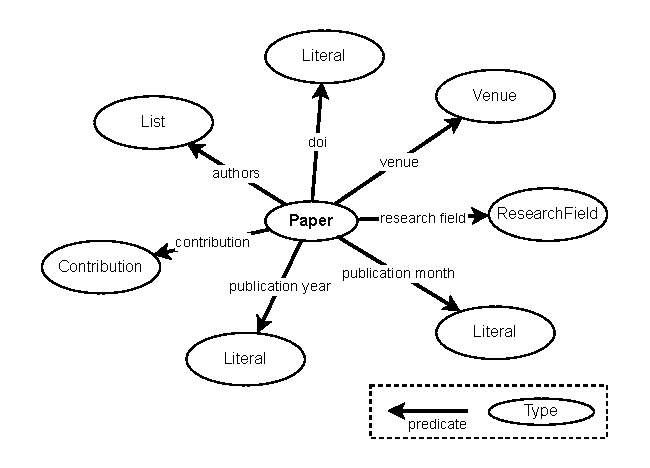
\includegraphics[width=0.7\linewidth]{figures/orkg/figures-orkg_structure.drawio.pdf}
    \caption[Schematic Representation of ORKG Publication Data]{Schematic representation of how publication data is structured in the ORKG, illustrating the root entity \emph{Paper} and its linkage to metadata and \emph{Contribution} entities.}
    \label{fig:orkg_structure}
\end{figure}

\paragraph{Storing Publications} As previously mentioned, scientific publications are represented in the \gls{orkg} using the \emph{paper} content type. Interaction with these paper entities forms the principal mode of engagement with the \gls{orkg} relevant to this thesis. \autoref{fig:orkg_structure} depicts the organizational structure for storing publication data. The diagram illustrates that the paper entity serves as the central node for publication information. All associated data, including metadata and one or more contributions detailing the research content, are linked to this paper entity using statements.

\subsection{The KARAGEN Approach for Question Answering on the ORKG}

\gls{karagen} is an approach for implementing a \gls{qa} system on the \gls{orkg} graph. The goal is to take advantage of the complementary strengths of \glspl{llm} and \gls{kg}. In this relationship, the \gls{kg} provides a structured data foundation in which information is stored in an interconnected network of entities and their relationships. The benefit of the graph is the ability to semantically link information, thus preserving the context and relationships between pieces of knowledge. On the other hand, \glspl{llm} excel in interpreting and generating natural language, with their advantage being that users can formulate their queries in natural language instead of relying on keyword-based queries. \cite{kaplan_combining_2024}

\begin{figure}[t]
    \centering
    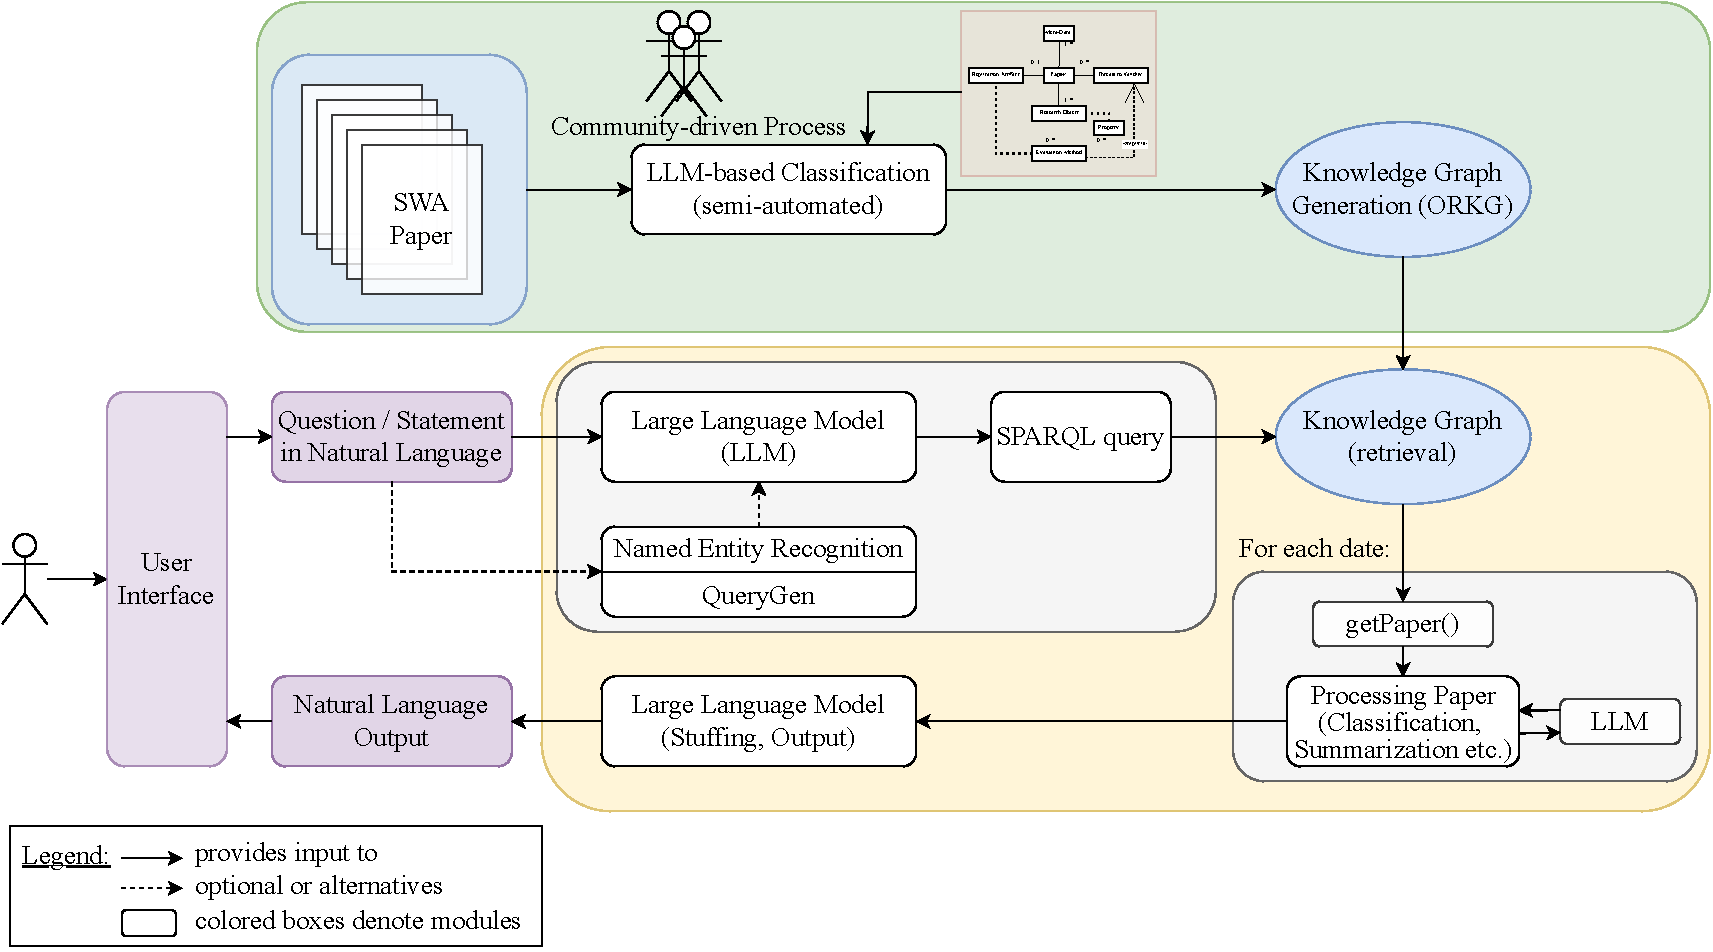
\includegraphics[width=0.95\textwidth]{figures/karagen.pdf}
    \caption[The KARAGEN Approach]{The KARAGEN approach, as proposed by \textcite{kaplan_combining_2024}, consists of two parts for a \gls{llm}-based retrieval on the \gls{orkg}. The green box shows the generation and population of the \gls{orkg}, while the yellow box depicts the \gls{llm}-based retrieval.}
    \label{fig:karagen}
\end{figure}

The \gls{karagen} approach is illustrated in \autoref{fig:karagen} and is composed of two parts: 1) Knowledge Graph Generation and Population and 2) Knowledge Retrieval. The following explanations are based on the descriptions provided by \textcite{kaplan_combining_2024}.

\paragraph{Knowledge Graph Generation and Population} This component is responsible for populating the \gls{orkg} with information through a semi-automated process, where users are supported by \gls{llm}-based classification. In the case of the \gls{orkg}, adding information about research papers is facilitated through templates. This means that either users or machines can fill in the required information into these templates, which are then stored in the graph as a contribution to the research paper.

\paragraph{Knowledge Retrieval} This component handles the retrieval and processing of knowledge from the graph. Users can submit queries in natural language, which are then processed using an \gls{llm}. The retrieval process may involve several steps, such as generating graph queries by matching natural language elements to graph components. Optionally, a knowledge enhancement component can be incorporated to transform and generate information. Finally, the system generates a response for the user. During this retrieval process, sources can be added to indicate the origin of the data and ensure traceability.

% In the following, we present the core concepts of the \gls{orkg}. This information is derived from \cite{ilangovan_open_2024} and the official \gls{orkg} website\footnote{\url{https://orkg.org/about} [last accessed on 21.12.2024]}.

% A recent study by \textcite{verma_scholarly_2023} reviewed 10 \glspl{rkg} that support scholarly infrastructures and found that nearly all used RDF for data representation. The study also highlighted that the core research-related entities across these graphs are quite similar, generally grouping into eight categories. The first group, \emph{People}, involves individuals such as authors and researchers. The second group, \emph{Publications}, relates to scholarly outputs like journal articles and conference papers. The third group, \emph{Organizations}, includes universities, research institutes, and other bodies that researchers belong to. The fourth group, \emph{Events}, covers academic gatherings like conferences and workshops. The fifth group, \emph{Datasets}, refers to digital collections or platforms where publications, data, and related resources are stored. The sixth group, \emph{Publishers \& Venues}, encompasses journals, conference venues, and other forms of publishers.

% TODO Add typical structure of a RKG \cite{verma_scholarly_2023}



% A \gls{kg} is an extended form of an ontology providing richer entity descriptions at the instance level \cite{ilangovan_open_2024}. 

% Mathematically speaking, a \gls{kg} stores structured knowledge as a collection of triples \(KG = \{(h,r,t) \subseteq \varepsilon \times R \times \varepsilon \} \), where \(\varepsilon\) denotes the entities and \(R\) the relation between the entities \cite{pan_unifying_2024}. These entities and their relationships are organized in a directed graph (\(G\)), defined as \(G = (V, E)\). In this graph, the vertices (\(V\)) correspond to the entities, and the edges (\(E\)) denote the relationships between them. Intuitively, a fact in the knowledge graph is formed by two entities connected by a relationship \cite{abu-salih_domain-specific_2021}.

% \Glspl{kg} have become an emerging technology in industry and in academia as they enable data to be organized \enquote{in a flexible, fine-grained, context-sensitive, and semantic representation to be understandable, processable, and usable by humans and machines \cite{karras_divide_2023}}.

% - A scholarly \gls{kg} is a type of graph that contains bibliographic information \cite{banerjee_dblp-quad_2023}. Some well known scholarly \glspl{kg} are the Microsoft Academic Graph, OpenAlex, ORKG, and DBLP.

% - The DBLP \gls{kg} includes bibliographic information on a wide range of topics within the field of computer science. It mainly consists of two entities \emph{Person} and \emph{Publication} \cite{banerjee_dblp-quad_2023}.  
% According to \textcite{taye_understanding_2010}, the semantic web aims to extend the current web by representing the information in both a human and machine-readable format. The backbone of the semantic web is formed by \emph{ontologies} by offering a shared conceptualization of a domain. An ontology consists of the following components:

% \begin{enumerate}
%     \item \emph{Concepts} are also referred to as classes or terms and represent abstract groups, sets, or collections of objects within a domain. They are organized hierarchically with parent and child relationships.
%     \item \emph{Instances} or individuals represent specific objects or elements of a concept.
%     \item \emph{Relations} or slots define how concepts are related to one another.
%     \item \emph{Axioms} are used to impose constraints on the values of concepts or instances. These are usually expressed in logic-based languages and ensure consistency within the ontology.
% \end{enumerate}

% \gls{rdf} is described as the first layer of the Semantic Web architecture \cite{taye_understanding_2010}. It provides the framework for representing metadata and semantics in a machine-readable format and can be applied to semi-formally describe ontologies. At the core of \gls{rdf} are triples, which are statements in the form of \((subject, predicate, object)\) \cite{wood_rdf_2014}. A \emph{subject} is the resource that is being defined, which can be either an \gls{iri} or a blank node. A \emph{predicate} is the property or relation between the subject and the object in the form of an \gls{iri}. The \emph{object} is the value or target of the relationship and can be either an \gls{iri}, a blank node, or a literal. A \gls{iri} acts as a unique identifier for resources, while literals are atomic pieces of information. Blank nodes are used to represent resources that do not have a unique identifier. 

% Combined as a set, triples form a \gls{rdf} graph which is a directed graph where the nodes represent entities and the edges represent the relationships between them \cite{hogan_knowledge_2022, paulheim_knowledge_2016, barrasa_building_2023}. When such a graph accumulates data to convey knowledge about the real world, making it comprehensible to both humans and machines, it is referred to as a \gls{kg}. 

\section{Knowledge Graph Question Answering (KGQA)}

\acrfull{kgqa} presents a research area that focuses on empowering users to access information stored within a \gls{kg} by formulating questions in natural language \cite{banerjee_knowledge_2024,chakraborty_introduction_2021,chakraborty_introduction_2019,pan_unifying_2024,yani_better_2022}. The primary objective of \gls{kgqa} is to retrieve answers from a \gls{kg} based on a question posed in natural language. This eliminates the necessity for users to write formal query languages such as SPARQL or possess intricate knowledge of the underlying structure and vocabulary of the \gls{kg} \cite{chakraborty_introduction_2021,chakraborty_introduction_2019,sabou_survey_2017}.

Historically, the research objective of enabling automated systems to answer questions posed in natural language precedes the modern adoption of \glspl{kg}. Early efforts in \acrfull{qa} explored systems designed to respond to questions by querying structured \acrfull{kb} or databases with early systems dating back to the 1970s and 1980s. A significant surge in interest in natural language question answering occurred with the establishment of a \gls{qa} track at the Text Retrieval Conferences (TREC), beginning in 1999. \cite{hirschman_natural_2001}

Due to advancements in semantic web technologies and automated information processing, the creation of large volumes of structured information became feasible \cite{chakraborty_introduction_2019}. \glspl{kg} emerged as a prime instance of storing structured data, which model facts about entities and their relationships, often in collections of triples \cite{chakraborty_introduction_2019,hogan_knowledge_2022,ji_survey_2022}. Consequently, \gls{kgqa} systems were developed to provide an intuitive natural language interface to query this structured knowledge contained in \glspl{kg}. Over time, several terms have been used for this task, including \acrfull{kbqa} \cite{ehrlinger_towards_2016} and \acrfull{sqa} \cite{sabou_survey_2017}. However, the term \gls{kb} has often been used misleadingly in the literature as a synonym for \glspl{kg} \cite{ehrlinger_towards_2016}.

 As \gls{kgqa} research progressed, the focus from simple questions requiring the retrieval of single facts shifted to more complex ones requiring multi-hop reasoning or constraints \cite{fu_survey_2020,banerjee_knowledge_2024,chakraborty_introduction_2021}. Two primary research directions emerged for building \gls{kgqa} systems: Methods based on \emph{\gls{ir}} gather question-related information from the \gls{kg} and leverage it to optimize the generation process. \emph{\gls{sp}-based methods} focus on the translation of the natural language question into a formal query or logical form that can be executed directly against the \gls{kg}.

 Neural networks became integral to various aspects of \gls{kgqa} systems across both \gls{ir} and \gls{sp} paradigms \cite{chakraborty_introduction_2019,ji_survey_2022}. Employed neural network architectures include embedding models, Recurrent Neural Networks (RNNs), Convolutional Neural Networks (CNNs), and Graph Neural Networks (GNNs) \cite{chakraborty_introduction_2021,pan_unifying_2024,ji_survey_2022}. More recently, the advent of pre-trained \glspl{llm} has begun to impact research on \gls{kgqa}. Although some research explores whether \glspl{llm} themselves can replace \glspl{kg}, most research is directed at the unification of \glspl{llm} and \glspl{kg} \cite{pan_unifying_2024}. In current research, \glspl{llm} are integrated into \gls{kgqa} systems in various ways. For instance, they can act as entity/relation extractors to extract data from questions, are used in \gls{sp} approaches to translate questions into formal queries, or are used in \gls{ir}-based approaches to function as reasoners over retrieved \gls{kg} subgraphs \cite{pan_unifying_2024}.


% Questions answered by KGQA systems are often divided into the categories—simple and complex. The questions, which can be answered by considering a single fact, without any additional constraints are generally defined as simple questions. For instance, the question “What is the birthplace of Michael Crichton” is a simple question since it can be answered by only considering the following fact: hex:Chicago, ex:birthPlaceOf, ex:Michael_Crichtoni. In contrast, the question “What is the birthplace of Westworld's writer?” is considered complex since answering this question requires knowing both hex:Michael_Crichton, ex:writerOf, ex:Westworldi and hex:Chicago, ex:birthPlaceOf, ex:Michael_Crichtoni. \cite{chakraborty_introduction_2021}

% In the QA community, KGQA is often also called knowledge base question answering (KBQA). \cite{chakraborty_introduction_2021}



% \acrfull{kgqa} is a relatively new research field with no established definition. In some works, \gls{kgqa} is used synonymously with \gls{kbqa} \cite{fu_survey_2020,peng_graph_2024}

\section{Large Language Models}
\label{sec:fundamentals_language_models}

\acrfullpl{llm} are pre-trained models with hundreds of billions of parameters generated by excessive training of very large corpora of text \cite{chung_scaling_2022}. These models are designed to estimate the probability distribution in a sequence of text, enabling them to perform a wide range of language-related tasks \cite{kojima_large_2023}. Recently, \glspl{llm} have demonstrated powerful capabilities in natural language understanding, expressiveness, general knowledge, and zero-shot generalization \cite{yang_give_2024}.

The architecture of most \glspl{llm} is derived from the \emph{Transformer} design, which includes encoder and decoder modules empowered by a self-attention mechanism \cite{pan_unifying_2024}. Based on their structure, \glspl{llm} can be broadly categorized into \emph{encoder-only}, \emph{decoder-only}, and \emph{encoder-decoder} models. Notable examples of these architectures are Flan T5 \cite{chung_scaling_2022} for the encoder-decoder framework, GPT-4 \cite{openai_gpt-4_2024} for the decoder-only framework, and DeBERTa \cite{he_deberta_2021} for the encoder-only framework. In this thesis, we focus on the decoder-only framework, as many state-of-the-art \glspl{llm} follow this architecture \cite{pan_unifying_2024}.

\subsection{Prompting} 
An important concept in leveraging \glspl{llm} is \emph{prompting}, which involves conditioning the model on a natural language instruction to guide its generation for desired tasks without any further training or gradient updates to its parameters \cite{wei_emergent_2022,kojima_large_2023}. Given this input prompt, the \gls{llm} then generates an answer in natural language. Popular prompting methods are \emph{few-shot prompting}, which involves adding a few examples \cite{brown_language_2020} or only adding instructions describing the task, which is referred to as \emph{zero-shot prompting} \cite{kojima_large_2023}. Another popular prompting method is Chain-of-Thought (CoT), where a chain-of-thought demonstration is provided during prompting \cite{wei_chain--thought_2023}. To maximize the effectiveness of \glspl{llm}, \emph{prompt engineering} is a new field that focuses on the creation and refinement of prompts \cite{pan_unifying_2024}.

\subsection{Limitations} 
Despite their impressive capabilities, \glspl{llm} face certain limitations. They are often described as black-box models, which means that they lack explainability and transparency, making it difficult for users to comprehend the reasoning behind their answers \cite{yang_give_2024,pan_unifying_2024}. Furthermore, \glspl{llm} are prone to generating factual errors or \emph{hallucinations} in which the \gls{llm} provides answers that contradict existing sources or lack evidence to support statements, which is particularly prominent when handling queries beyond their training data or when requiring current information \cite{gao_retrieval-augmented_2024,yang_give_2024}. Moreover, \glspl{llm} may not perform as well on domain-specific tasks as on general ones due to the limited availability of domain-specific corpus \cite{yang_give_2024}.

\subsection{Embedding Models}

A challenge concerning natural language processing is the representation of words and their associated meanings. One paradigm to approach this challenge is the use of vector representations in a continuous space. The fundamental idea behind these representations is that words that appear in similar contexts tend to have similar meanings. Consequently, within such a vector space, the proximity between word representations encodes semantic and syntactic regularities. These dense vectors are typically referred to as \emph{embeddings}. \cite{banerjee_knowledge_2024, pennington_glove_2014, mikolov_efficient_2013}

Early methods for learning representations of words, such as Word2Vec \cite{mikolov_efficient_2013} and GloVe \cite{pennington_glove_2014}, train word embeddings based on the co-occurrence statistics of words within a large text corpus. This class of embeddings is termed \emph{static} because the matrix produced during training is used without alteration. To address this limitation, \emph{dynamic} word embeddings utilize the advances of the transformer model to compute different representations for the same word depending on its context within the given sentence. Consequently, transformer-based pre-trained language models such as BERT \cite{devlin_bert_2019} have become relevant to solving the challenge of word representation. \cite{banerjee_knowledge_2024}


% \subsection{Graph Integration}
% Given these limitations and the complementary strengths of \glspl{kg} which explicitly store rich factual knowledge in a structured format, unifying \glspl{llm} and \glspl{kg} has become an active research direction \cite{pan_unifying_2024,peng_graph_2024}. Such a unification aims to leverage the advantages of both, enhancing the factual reasoning and interpretability of \gls{llm} answers while potentially using \glspl{llm} to aid in \gls{kg} construction and evolution \cite{pan_unifying_2024}.
 




% \subsection{Large Language Models}
% Research on PLMs has shown great success in scaling the model, which improves the capabilities of the model in downstream tasks, leading to surprising emerging abilities. Examples for such abilities that are not present in small models but arise in very large models are few-shot prompting, instruction following, and chain-of-thought \cite{wei_emergent_2022}.  

% Scaling PLMs to a certain threshold that emits these abilities is what distinguishes PLMs from \glspl{llm} \cite{yang_give_2024}. 

% This means that typically \glspl{llm} refer to PLMs that consist of hundreds of billions of parameters, with notable examples being: Flan T5 \cite{chung_scaling_2022} for the encoder-decoder framework, GPT-4 \cite{openai_gpt-4_2024} for the decoder-only framework, and DeBERTa \cite{he_deberta_2021} for the encoder-only framework. 

% 

% \subsection{Categorization}
% The architectural framework used in a PLM can be categorized into three types: encoder-only, decoder-only, and encoder-decoder \cite{wang_pre-trained_2023}. 

% \paragraph{Decoder-Only} 
% In the decoder-only approach, a unidirectional transformer decoder, operating from left to right, serves as the foundational mechanism during pre-training. This method employs an autoregressive technique for token prediction, in which each token is predicted based on its preceding tokens. Specifically, given a text sequence \(x = (x_1, x_2, x_3, ..., x_T)\), where \(x\) is the complete original sentence, \(x_t\) is the t-th token, and \(T\) is the total number of tokens, the model computes the probability of the sequence by the product \(p(x) = \prod^T_{t=1}p(x_t|x_{<t})\), representing the probability of each token given its previous sequence.

% \paragraph{Encoder-Only}
% Frameworks based on transformer encoders, such as the one used by BERT, employ bidirectional transformers to address the challenge of restoring altered tokens within sentences containing randomly masked elements. BERT exemplifies this approach through its use of a Masked Language Model (MLM) methodology, where specific tokens are substituted with a [MASK] token during the pre-training phase. The model then uses the surrounding contextual information to accurately predict the original tokens. Furthermore, BERT enhances its comprehension of text relationships by employing a Next Sentence Prediction (NSP) technique, which evaluates the links between consecutive sentences. This feature is beneficial for tasks that necessitate grasping sentence contexts, such as question answering.

% \paragraph{Encoder-Decoder}
% The encoder-decoder framework is tailored for training sequence-to-sequence (seq2seq) models. This process involves obscuring tokens within the source sequence and subsequently reconstructing them in the target sequence. Broadly, these frameworks are differentiated into two distinct types: 1) the seq2seq encoder-decoders, which integrate a bidirectional transformer encoder with a unidirectional transformer decoder, each posing independent parameters; and 2) the unified encoder-decoders, where both the bidirectional encoder and the unidirectional decoder are trained concurrently with the same set of parameters. This architecture is primarily devoted to tasks in natural language generation (NLG), as it equips the model to simultaneously manage tasks related to understanding and generating language.


\section{Graph Retrieval Augmented Generation (GraphRAG)}

 The paradigm of \acrfull{rag} has gained significant traction to mitigate issues with \glspl{llm}, such as hallucination, lack of domain-specific knowledge, and outdated information. The concept behind \gls{rag} is to improve the outputs of an \gls{llm} by providing it with relevant information retrieved from an external knowledge source at the time of inference instead of relying on the potentially outdated or imprecise knowledge internalized during pre-training. \cite{lewis_retrieval-augmented_2021,wu_retrieval-augmented_2024,peng_graph_2024,yang_give_2024}

A typical \gls{rag} system involves a \emph{retriever} component that obtains relevant information from a \gls{kb} and a \emph{generator} component that uses an \gls{llm} to generate a response based on the information retrieved and the question \cite{wu_retrieval-augmented_2024,yu_evaluation_2024}.

\acrfull{grag} represents an instantiation of the \gls{rag} paradigm where instead of retrieving information from unstructured text documents, \gls{grag} specifically targets and retrieves structured knowledge from graph databases such as \glspl{kg} or text-attributed graphs \cite{peng_graph_2024}. Consequently, \gls{grag} is positioned at the intersection of several key areas: traditional \gls{kgqa}, the \gls{rag} paradigm, and the emerging field of unifying \glspl{llm} and \glspl{kg} \cite{pan_unifying_2024,peng_graph_2024}.

A typical workflow of \gls{grag} comprises three main stages \cite{peng_graph_2024}:

\begin{enumerate}
    \item \textbf{Graph-based Indexing:} This constitutes the initial phase of \gls{grag}, where a pre-existing graph database is selected or constructed to then establish indices upon it to later facilitate efficient retrieval.
    \item \textbf{Graph-Guided Retrieval:} Given the provided input question, this phase aims to identify and extract a relevant subset of the graph data that is useful to provide an answer to the question.
    \item \textbf{Graph-Enhanced Generation:} In this final stage, the question and the retrieved graph knowledge are used as input for an \gls{llm} to produce the natural language response.
\end{enumerate}


% Authoren die RAG initial vorgestellt haben: \cite{lewis_retrieval-augmented_2021}
% Ein gutes Survey für RAG \cite{gao_retrieval-augmented_2024}
% Since the emergence of \glspl{llm}, a growing number of research has focused on \gls{rag} \cite{gao_retrieval-augmented_2024}.

% According to \textcite{yu_evaluation_2024} a typical \gls{rag} system comprises two main components: \emph{Retrieval} and \emph{Generation}. The purpose of the retrieval component is to extract information from \glspl{kb} that is relevant to a given query. There are two primary phases involved during retrieval: \emph{indexing} and \emph{searching}. 

% The searching phase is responsible for the retrieval of relevant information based on a given query. It can be categorized into three types: \emph{sparse retrieval}, \emph{dense retrieval}, and \emph{web search engine}. Sparse retrievers assess the similarity between the query and documents through weighted term matching and are not trained on specific data distributions. Typical methods are TF-IDF \cite{ramos_using_2003} and BM25 \cite{robertson_probabilistic_2009} which rely on keyword matching and word frequency. Although they excel at lexical matching, they do not recognize synonyms and paraphrases and therefore miss relevant context without keyword overlap. In contrast, dense retrievers evaluate similarity by employing representations learned from supervised QA datasets and leveraging pre-trained language models such as BERT \cite{he_deberta_2021} or GPT-4 \cite{openai_gpt-4_2024}. This capability enables them to identify relevant documents even with minimal keyword overlap, which is essential for complex queries that require contextual understanding. Lastly, retrieval over web search engine allows the retriever to traverse the extensive information in the web using search engines like Google Search\footnote{\url{https://developers.google.com/custom-search/v1/overview} [last accessed on 11.01.2025]} or Bing Search\footnote{\url{https://www.microsoft.com/en-us/bing/apis/bing-web-search-api} [last accessed on 11.01.2025]}. 

% Indexing is a preprocessing step that is performed before the search to organize information in a way that allows efficient retrieval. For sparse retrieval indexing involves the calculation of IDF for each term and storing the values in a database for a quick look-up and scoring when queried. Dense retrieval, on the other hand, encodes the information into dense vectors through the use of a pre-trained language model. The vectors are then indexed using a \gls{ann} search technique \cite{douze_faiss_2024}. For indexing large documents, the technique of chunking is frequently employed. It restricts similarity scores to specific segments instead of the entire text. This approach is particularly beneficial, as semantic embeddings tend to be less accurate for lengthy documents. Moreover, the information requested frequently tends to be brief in nature.

% The contexts retrieved during the search step are then used in the generation component of the \gls{rag} system to generate a final answer to the query. \textcite{yu_evaluation_2024} underscore the significance of prompting as a fundamental aspect upon which the generation process heavily relies. In the process of generation prompting, the query, relevant retrieval contexts, and instructions are combined into one comprehensive input for the \gls{llm} to utilize. The literature suggests various prompting techniques that may be employed to shape the output of the model. \gls{cot} encourages the model to generate a step-by-step reasoning process before arriving at a final answer \cite{wei_chain--thought_2023}. \gls{tot} extends the idea of \gls{cot} by exploring multiple lines of reasoning simultaneously, creating a tree of possible thought processes \cite{besta_graph_2024}. Self-Note involves the model to explicitly think and write down its thoughts \cite{lanchantin_learning_2023}. The \gls{rar} prompting strategy first rephrases and rewrites the user query before formulating a response \cite{deng_rephrase_2024}.

% In addition, after the generation of the final output, a post-processing step may be implemented where the output is formated according to the specific needs of the task or an expected output structure \cite{yu_evaluation_2024}.

% \subsection{Definition of GraphRAG}

% TODO: Transition from RAG to GRAPHRAG

% "From a broad perspective, GraphRAG can be seen as a branch of RAG, which retrieves relevant relational knowledge from graph databases instead of text corpus. However, compared to textbased RAG, GraphRAG takes into account the relationships between texts and incorporates the structural information as additional knowledge beyond text. Furthermore, during the construction of graph data, raw text data may undergo filtering and summarization processes, enhancing the refinement of information within the graph data." \cite{peng_graph_2024}

% \subsection{Categories of GraphRAG Approaches}
% \label{sec:categories_of_graphrag_approaches}

% \begin{table}[t]
%     \centering
%     \renewcommand{\arraystretch}{1.5}
%     \begin{tabular}{p{3cm}lp{4cm}p{4cm}}
%         \toprule
%         \textbf{Category} & \textbf{Type} & \textbf{Strengths} & \textbf{Weaknesses} \\ 
%         \midrule
%         \multirow{3}{*}{\textbf{Models}}         
%             & Non-parametric & Fast, low cost & Low accuracy \\ 
%             & LM-based & Accurate, handles natural queries & High computational cost\\ 
%             & GNN-based & Leverages graph structure & Complex to implement\\ 
%         \midrule
%         \multirow{3}{*}{\textbf{Paradigms}}      
%             & Once retrieval & Fast, low complexity & Limited scope \\ 
%             & Iterative retrieval & Adaptive, high accuracy & Longer runtime\\ 
%             & Multi-stage retrieval & Task-specific, modular & Requires careful design\\ 
%         \midrule
%         \multirow{4}{*}{\textbf{Granularity}}   
%             & Node-based & Targeted retrieval & Lacks relational context\\ 
%             & Triplet-based & Handles relationships & Limited to triple scope\\ 
%             & Path-based & Captures sequences & High computational load\\ 
%             & Subgraph-based & Comprehensive retrieval & Complex and costly\\
%         \midrule
%         \multirow{2}{*}{\textbf{Training Strategy}}   
%             & Training-Free & Avoiding high training costs & Careful prompt engineering \\ 
%             & Training-Based & Adaptive to specific tasks & Requires costly training\\ 
%         \midrule
%         \multirow{2}{*}{\textbf{Indexing}}   
%             & Graph Indexing & Preserves graph structure & Long retrieval times \\
%             & Text Indexing & Simple textual content retrieval & Limited to text-based queries\\
%             & Vector Indexing & Quick and efficient search & Requires vectorization \\
%             & Hybrid Indexing & Combines advantages of other methods & Complex to implement \\
%         \bottomrule
%     \end{tabular}
%     \caption{Comparison of GraphRAG categories according to \cite{peng_graph_2024}}
%     \label{tab:retrieval_comparison}
% \end{table}

% To better understand the landscape of \gls{grag} approaches proposed by the literature, researchers have proposed different taxonomies to categorize these approaches. In this section, we examine two prominent taxonomies: one proposed by \textcite{peng_graph_2024} that focuses on technical aspects like models and retrieval strategies, and another by \textcite{pan_unifying_2024} that emphasizes the integration between \glspl{llm} and \glspl{kg}.

% \textcite{peng_graph_2024} propose to categorize the approaches based on the underlying \emph{Model}, \emph{Retrieval Paradigm}, \emph{Retrieval Granularity}, \emph{Training Strategy}, and \emph{Indexing}. Table \ref{tab:retrieval_comparison} provides an overview of the categories, highlighting the strengths and weaknesses of each category.

% \paragraph{Model Categorization} Retrievers can be categorized into three types, based on their underlying models. The \emph{Non-parametric} retriever type is based on heuristic rules or traditional graph search algorithms. They often include a linking pre-processing step to identify nodes in the graph before the retrieval. Because these methods are not using deep-learning models, they are able to achieve fast retrieval times with low costs. However, they suffer from inaccurate retrieval. The \emph{LM-based} retriever, on the other hand, shows strong performance in processing and interpreting diverse natural language queries. They are based on pre-trained language models like GPT-4 \cite{openai_gpt-4_2024}, and can be further categorized into two types: discriminative and generative. The discriminative models focus on estimating the conditional probability and are effective in task such as text classification and sentiment analysis. Discriminative models, on the other hand, show great potential in language understanding and in-context learning. While LM-based retrievers offer a higher retrieval accuracy, they require significantly more computational overhead compared to the Non-parametric retrievers. The third type, the \emph{GNN-based} retriever, utilizes a GNN model to understand and leverage complex graph structure. They typically encode the graph data and subsequently score different retrieval granularities based on their similarity to the query.

% \paragraph{Retrieval Paradigm} Additionally, GraphRAG retrievers can be categorized based on the retrieval paradigm they employ. This categorization classifies retrievers according to how frequently they access information in the graph and whether there are phases during which the information is processed. There are three paradigms: once retrieval, iterative retrieval, and multi-stage retrieval.
% \emph{Once retrieval} refers to retrievers that access the graph with only a single query to obtain all the information required for the retrieval process. Examples of this approach include embedding-based methods or those that use predefined rules or patterns to formulate queries to the graph. The once retrieval paradigm is typically faster as it involves lower complexity.
% \emph{Iterative retrieval}, on the other hand, refers to retrievers that access the graph multiple times to gather the information needed for the retrieval process. Here, several retrieval steps are executed sequentially, with each subsequent step depending on the results of the previous retrieval step. This approach can be either adaptive, for instance, when models autonomously decide which steps to execute next and when to terminate the retrieval process, or non-adaptive when the steps are predetermined and termination is based on predefined parameters. The iterative paradigm generally has longer runtimes, especially when \glspl{llm} are used, but offers higher accuracy.
% Lastly, there is the \emph{multi-stage retrieval} paradigm. In this paradigm, the retrieval process is divided into multiple phases, each with a different task. For example, different retrieval methods can be used in different phases, or generation processes can be integrated into the retrieval process.

% \paragraph{Retrieval Granularity} Furthermore, retrievers can be categorized based on the retrieval granularity they use. The retrieval granularity refers to the level of detail at which the retriever retrieves information from the graph. There are four types of granularities proposed by \textcite{peng_graph_2024}: Nodes, Triplets, Paths, and Subgraphs. \emph{Node-based retrievers} retrieve information at the node level, which means that they retrieve information from individual elements in the graph. This is ideal for targeted queries where specific information from the graph should be extracted. \emph{Triplet-based retrievers} retrieve information at the triplet level, which consists of both the nodes and their relationships in the form of subject-predicate-object tuples. This granularity is useful for queries that require information about the relationships between nodes, for example, when contextual relevance between entities is required. When sequences of relationships between entities are required, \emph{Path-based retrievers} are used. However, for comprehensive relational contexts within a graph, a \emph{Subgraph-based retriever} might be required. 

% \paragraph{Training Strategy} In the classification of retrievers based on their training strategy, a distinction is made between Training-Free and Training-Based Retrievers. \emph{Training-Free Retrievers} are retrievers that do not require a training phase and can be applied directly to the graph. Retrievers of this category often rely on carefully defined prompts, as \glspl{llm} like GPT-4 \cite{openai_gpt-4_2024} are frequently used. There are several sub-categories of Training-Free Retrievers. Non-parametric retrievers operate with predefined rules or traditional graph search algorithms and do not use specialized models. On the other hand, there are retrievers that work with pre-trained \glspl{llm}. For example, pre-trained embedding models are used, which are applied to the graph in an indexing step. Additionally, there are approaches that send graph elements such as entities, triples, paths, or subgraphs as part of a prompt to an \gls{llm} to obtain a selection or answer. \emph{Training-Based Retrievers}, on the contrary, require a training or fine-tuning phase in which supervised signals are used. However, these variants are often challenging because they require ground truth data, which is frequently unavailable.

% \paragraph{Indexing} The retrieval approaches can also be categorized based on the indexing strategy they use. There are four types of indexing strategies: Graph Indexing, Text Indexing, Vector Indexing, and Hybrid Indexing. \emph{Graph Indexing} preserves the entire structure of the graph. It is often seen in conjunction with classic graph search algorithms such as BFS and Shortest Path algorithms. \emph{Text Indexing} involves to convert the graph structures to textual representations which are then stored in a corpus. Various sparse and dense retrieval techniques are applied to retrieve the relevant information. \emph{Vector Indexing} directly transforms the structures of the graph into vectors which are then stored in a database. Finally, \emph{Hybrid Indexing} is a combination of the three indexing strategies mentioned above.

% Another taxonomy is proposed by \textcite{pan_unifying_2024}. They focus on the unification of \glspl{llm} with \glspl{kg} to synergize the advantages of both technologies. The taxonomy includes various tasks such as incorporating the \glspl{kg} into the \gls{llm} during pre-training, fine-tuning, and inference. They also consider to use the \gls{llm} to improve the \gls{kg} by enriching the graph representation. In the following we are going to look at the proposed categories for retrieval in a \gls{qa} setting.

% \paragraph{KG-enhanced LLM inference} categorizes research that uses \glspl{kg} during the inference stage of \glspl{llm}. These methods do not require to retrain the model as they add up-to-date information to the \gls{llm} at inference time. A popular method to inject this knowledge is articulated by the authors as \emph{Retrieval-Augmented Knowledge Fusion}. Here, relevant knowledge is retrieved from a large corpus and then fused into the \gls{llm} during inference. Another method is \emph{KGs Prompting}. Here, the structure of the \gls{kg} is added to the prompt during inference to guide the \gls{llm} in generating the answer. The challenge in this category is to carefully design a prompt that converts the structured graph information into text sequences that the \gls{llm} can understand. 

% \paragraph{LLM-augmented KG Embedding} focuses on methods that map each entity and relation into a low-dimensional vector space. By applying this approach, the embeddings contain both the semantic kownloedge and structural information of the \gls{kg}. These embeddings are then used in tasks such as \gls{qa}, reasoning, and recommendation. There are two subcategories in this category: \emph{LLMs as Text Encoders} and \emph{LLMs for Joint Text and KG Embedding}. The former uses a embedding model to encode the textual information of the \gls{kg} into embeddings, while the latter directly encodes both the textual information and the graph structure into embeddings by training the \gls{llm}.

% \paragraph{LLM-augmented KG Question Answering} has the aim to provide answers to natural language questions based on the facts that are stored in the \gls{kg}. There are two subcategories in this category: First \emph{LLMs as Entity/Relation Extractors} has the goal to identify and extract entities and relationships that are mentioned in the natural language question to then retrieve relevant facts from the \gls{kg} based on this extraction. The second subcategory is \emph{LLMs as Answer Reasoners}. In this category, the facts are already retrieved from the graph and the goal is to reason over these facts to generate the answer to the question.

% \paragraph{Synergized Reasoning} includes methods that design synergized models capable of leveraging both the representational power of \glspl{llm} and the structured, relational knowledge of \glspl{kg} to perform complex reasoning. Notably, synergized reasoning often uses carefully designed architectures or joint training objectives to balance the benefits of continuous text-based representations with the discrete relational structures from \glspl{kg}. There are two subcategories in this category: First, \emph{LLM-KG Fusion Reasoning} adopts end-to-end trained \gls{llm} and \gls{kg} encoders to represent the knowledge in a unified space. Then a synergized reasoning module is applied to jointly infer answers. Second, \emph{LLMs as Agents Reasoning} employ the \gls{llm} itself as an active agent to retrieve and reason over graph-based knowledge without requiring additional training costs.



% To be able to find answers to a given question in a \gls{kg}, the user needs to have a in-depth understanding of the structure of the graph and its query language \cite{tran_comparative_2022}. To ease the access to information in a \gls{kg}, a significant effort has been put into building \gls{qa} systems that allow users to express their questions in natural language and for the system to find the relevant information for the user \cite{tran_comparative_2022}\cite{pang_survey_2022}\cite{bouziane_question_2015}\cite{thambi_towards_2022}\cite{liu_question_2015}.

% A \gls{kg} retriever refers to a methodology that retrieves relevant information from a \gls{kg}. Information is relevant, when it helps to answer a given question. 
% TODO: Add a bit of history to how the retrieval evolved
% mathematiccaly describe the problem: https://arxiv.org/pdf/2202.13296

% Warum gerade "LLMs to guide the retreival process". Vor- und Nachteile? Welche Alternativen gibt es hier noch das umzusetzen?
% In the context of this thesis, we refer to retrievers that retrieve information from a \gls{kg} based on a specified question while using a\gls{llm} to guide the retrieval process, as \gls{kglmqa} retrievers.
% TODO: Ausformulieren


% \begin{definition}[Topic Entity]
% \label{def:topic_entity}
% \leftskip=2em
%     The Topic Entity refers to an entity within the graph that serves as the starting node for the retrieval process. The retriever begins its traversal from this entity to locate relevant information corresponding to a specific query.
% \end{definition}

% \subsection{Multi-Hop Retrieval issue}

% Queries that require the retriever to reason and retrieve multiple contexts from the \gls{kb} is referred to as \emph{multi-hop} retrieval. This differs from single-hop queries where the answer can be directly derived from a single piece of context \cite{tang_multihop-rag_2024}. 

% Due to the multifaceted nature of such queries, multi-hop retrieval is a challenging task as traditional similarity matching methods like cosine similarity might not yield optimal results \cite{tang_multihop-rag_2024}.



% As shown in the study by \textcite{yu_decaf_2023}, current \gls{llm} based retrievers on \glspl{kg} struggle with multi-fact retrieval. 

\section{Approximate Nearest Neighbor (ANN) Search}
\label{sec:fundamentals_ann_search}

\acrfull{ann} search is a technique used to find data points that are likely close or similar to a given query point in a high-dimensional vector space. Unlike \gls{enn} search, which guarantees finding the absolute closest data points, \gls{ann} search trades some accuracy for significantly improved efficiency and speed \cite{douze_faiss_2024,wu_retrieval-augmented_2024}. The core idea behind \gls{ann} search is to preprocess the data into an indexing structure that tries to achieve a trade-off between search quality and search efficiency \cite{wu_retrieval-augmented_2024}. 
% Techniques include choosing appropriate distance metrics and advanced \gls{ann} indexing algorithms.

To understand the value of \gls{ann} search, it is helpful to first consider \gls{enn} search. Given a dataset of vectors ${x_i, i=1..N} \subset \mathbb{R}^d$ and a query vector $q \in \mathbb{R}^d$, a typical \gls{enn} search involves finding the index $n$ of the database vector $x_n$ that minimizes the distance to $q$, typically using a distance metric such as the Euclidean Distance (L2). Other popular similarity metrics are cosine similarity or inner product similarity, for which the objective would be to maximize the score. \cite{douze_faiss_2024}

A straightforward technique for \gls{enn} search is brute force, which involves calculating the distance between the query vector $q$ and every single database vector $x_i$ and then identifying one or more vectors with the smallest distance. The amount of vectors is often denoted by a $k$ parameter. However, this process is slow on large datasets where \gls{ann} search comes in handy. Here, database vectors are preprocessed in a specialized indexing structure to allow for quickly narrowing down the search space at query time. \cite{douze_faiss_2024,wu_retrieval-augmented_2024}

Various different \gls{ann} indexing techniques exist. \emph{Inverted File System with Product Quantization (IVFPQ)} involves the partitioning of the vector space by applying clustering algorithms to then use fine-grained quantization to compress the vectors. \emph{The Hierarchical Navigable Small World (HNSW)} is a technique that builds hierarchical graph structures where each node represents a vector. \emph{Tree-based Indexing} organizes the vectors into hierarchical tree-like structures to separate the vector space. \cite{wu_retrieval-augmented_2024}



% The accuracy of ANNS is typically measured as a discrepancy with exact search results. For k-nearest neighbour search, a common metric is "n-recall@k," which is the fraction of the true n nearest neighbors found within the k first search results. \cite{douze_faiss_2024}



\section{Evaluation Metrics}
\label{sec:fundamentals_evaluation_rag}

To evaluate \gls{grag} approaches, the evaluation metrics can be broadly categorized into two types: \emph{generation} and \emph{retrieval} quality \cite{peng_graph_2024,yu_evaluation_2024}. Evaluating the generation quality is about the assessment of the generated answer, while the retrieval quality is about the of retrieved information and the coverage of the answer.


\subsection{Evaluating the Retrieval Component}

The evaluation of retrievers dates back to early information retrieval research. Conventional metrics typically compare the retrieved contexts with a set of \emph{golden-labeled} contexts. These metrics fall into two types: \emph{Rank-agnostic} or \emph{Rank-aware}, depending on whether they consider the order in which the contexts are retrieved \cite{yu_evaluation_2024,alinejad_evaluating_2024}. In the following, we introduce commonly used metrics based on  \textcite{yu_evaluation_2024, ibrahim_survey_2024,hu_unveiling_2024}.

\paragraph{Rank-agnostic Metrics} These metrics measure the quality of retrieval without considering the position of the item in the list of retrieved contexts. 

\begin{itemize}
    \item \textbf{Accuracy:} An assessment of the ratio of correctly retrieved contexts compared to the total number of retrieved contexts.
    
    \[
    \text{Accuracy} = \frac{TP + TN}{TP + TN + FP + FN}
    \]

    \gls{tp} refers to contexts that are relevant to the query and are accurately retrieved. \gls{tn} refers to contexts that are irrelevant to the query and have not been retrieved. \gls{fp} refers to contexts that are irrelevant to the query but have been incorrectly retrieved. \gls{fn} refers to contexts that are relevant to the query but have not been retrieved.

    \item \textbf{Precision:} Measures the proportion of relevant contexts retrieved by the system to the total number of contexts retrieved by the system.
    
    \[
    \text{Precision} = \frac{TP}{TP + FP}
    \]

    \item \textbf{Recall:} Quantifies the proportion of relevant contexts that have been retrieved from the total number of relevant contexts for a given query, considering the top \(k\) results.
    
    \[
    \text{Recall} = \frac{TP}{TP + FN}
    \]

    \item \textbf{F1:} An assessment which calculates the harmonic mean of precision and recall.

    \[
    \text{F1} = 2 \times \frac{Precision \times Recall}{Precision + Recall}
    \]
\end{itemize}


\paragraph{Rank-aware Metrics} These metrics additionally evaluate the order in which relevant items are presented. Typically, the higher the relevant item is placed in the list, the better the score.

\begin{itemize}
    \item \textbf{Hits@k} A measure of the fraction of correct retrieved contexts that appear in the top \(k\) total of retrieved contexts.
    \[
    \text{Hits@k} = \frac{H_k}{N_{query}}.
    \]
    In the above formula, \( H_k \) is the number of times a relevant context entry is in the top-k and \(N_{query}\) is the total amount of retrieved context.

    \item \textbf{Mean Reciprocal Rank (MRR)} Measures the average of the inverse ranks of the first relevant context retrieved by the system. This means that the metric focuses on how high the retriever ranks the first relevant context.
    \[
    MRR = \frac{1}{|Q|} \sum^{|Q|}_{i=1} \frac{1}{rank_i}
    \]
    In the formula given above, \(|Q|\) represents the total number of queries, and \(rank_i\) denotes the rank position of the first relevant document for the \(i\)-th query.
    
    \item \textbf{Mean Average Precision (MAP)} Computes the average of the precision values at different cut-off points for each query. Consequently, this metric gives an aggregate view on how well the retriever ranks the relevant contexts.
    \[
    MAP =  \frac{1}{|Q|} \sum^{|Q|}_{q=1} \frac{\sum^n_{k=1} (P(k) \times rel(k))}{|relevant \space documents_q|} 
    \]
    In the formula given above, \(P(k)\) represents the precision at position \(k\) in the ranking list, and \(rel(k)\) is an indicator function that is one if the document at rank \(k\) is relevant and zero otherwise. In addition, \(n\) denotes the total number of documents retrieved.

    \item \textbf{Exact Match (EM)} quantifies the proportion of retrieved contexts that exactly match the expected contexts.
    \[
    Exact Match = \frac{PEM}{N_{pred}}
    \]
    Where in the formula \(PEM\) is the proportion of the exact matches and \((N_{pred}\) is the total number of expected contexts.
\end{itemize}


\subsection{Evaluating the Generation Component}

To assess the quality of the generated answer, often traditional metrics are borrowed from other natural language processing tasks like machine translation or summarization \textcite{yu_evaluation_2024,ibrahim_survey_2024,alinejad_evaluating_2024,alinejad_evaluating_2024}. However, these metrics often fail to fully capture the performance within an \gls{llm}-based \gls{qa} system \cite{alinejad_evaluating_2024}. Consequently, \gls{llm} models are employed as evaluative judges to assess the quality of generated answers \cite{es_ragas_2023}.

\paragraph{Traditional Natural Language Processing Generation Metrics} Common metrics that are applied to the evaluation in \gls{rag} are \textcite{yu_evaluation_2024,ibrahim_survey_2024,alinejad_evaluating_2024,alinejad_evaluating_2024}:

\begin{itemize}
    \item \textbf{ROUGE} \gls{rouge} is a set of metrics that evaluate the quality of the generated text by comparing it to the ground truth. There are multiple variants available: \gls{rouge}-N calculates recall by comparing the presence of n-grams in the generated text and the ground truth. \gls{rouge}-L uses the longest common subsequence to capture meaning in the generated text. \gls{rouge}-W additionally uses weights for consecutive matches, distinguishing between spatially aligned and scattered matches. \gls{rouge}-S incorporates skip-bigrams to balance flexibility and structure sensitivity. \gls{rouge}-SU is a variant of \gls{rouge}-S that uses skip-bigrams and unigrams to evaluate the quality of the generated text \cite{lin_rouge_2004}.

    \item \textbf{BLEU} The \acrfull{bleu} metric measures the quality of the generated text by comparing it with the ground truth by calculating the overlap of n-grams\cite{papineni_bleu_2001}. The \gls{bleu} score is calculated as:
    \[
    BLEU = BP \cdot \exp\left(\sum^N_{n=1} w_n \log p_n\right)
    \]
    In this formula, \(BP\) is the brevity penalty that penalizes short-generated translations, \(w_n\) is the weight for the n-gram, and \(p_n\) is the precision of the n-grams that match the reference.

    \item \textbf{BertScore} This metric uses contextual embeddings that, unlike n-gram-based metrics, capture the semantic meaning of the generated text. BertScore uses pre-trained transformer models like Bert to transform the generated text and the ground truth into embeddings. With the embeddings, the cosine similarity between the generated text and the ground truth is calculated, resulting in precision, recall, and f1 scores \cite{zhang_bertscore_2020}

\end{itemize}

\paragraph{LLM as a Judge Metrics} \glspl{llm} can be prompted with an evaluation scheme to assess the answers based on user-defined metrics. They have shown a great ability to capture semantic nuances and attend to variations in answers \cite{alinejad_evaluating_2024,yu_evaluation_2024}. Recently, a framework has been established focused on providing different \gls{llm}-based metrics \cite{es_ragas_2023}. Their framework is available online\footnote{\url{https://github.com/explodinggradients/ragas} [last accessed on 26.03.2025]} from which the following metric explanations have been taken from:

\begin{itemize}
    \item \textbf{Faithfulness} Measures the factual consistency of the generated answer against the given context, where the answer is regarded as faithful if all the claims made by the answer can be inferred from the given context.
    \[
    \text{Faithfulness} = \frac{\text{Number of supported claims}}{\text{Total number of claims}}
    \]

    \item \textbf{Answer Relevancy} Focuses on how relevant the answer is to the question where higher scores indicate better alignment while lower scores are given if the answer is incomplete or includes redundant information. To calculate the score, an \gls{llm} generates $N$ questions based on the generated answer and then calculates the cosine similarity between the actual question and the generated questions.
    \[
    \text{Answer Relevancy} = \frac{1}{N}\sum^N_{i=1}\text{cosine similarity}(E_{g_i},E_o)
    \]
    Where $N$ denotes the number of generated questions, $E_{g_i}$ the embedding of the i-th generated question, and $E_o$ is the embedding of the actual question.

    \item \textbf{Factual Correctness} evaluates how well the generated answer aligns with a golden reference. The \gls{llm} decomposes both answers into individual claims and computes \gls{tp}, \gls{fp}, and \gls{fn} as follows:
    \[
    \begin{aligned}
    \text{True Positives (TP)} &= \text{Claims in the answer also found in the reference} \\
    \text{False Positives (FP)} &= \text{Claims in the answer not found in the reference} \\
    \text{False Negatives (FN)} &= \text{Claims in the reference not found in the answer}
    \end{aligned}
    \]
    Precision, recall, and F1 scores are then calculated using these values, as defined above.
\end{itemize}


\subsection{Micro vs. Macro Averaging}
When evaluating the performance of systems across a dataset of multiple questions, the overall performance needs to be assessed through aggregation. There exist two common types of aggregate scores: \emph{micro-averaging} and \emph{macro-averaging} \cite{hu_unveiling_2024}:

\begin{enumerate}
    \item \textbf{Micro-Averaging} calculates the aggregation of metrics globally, for example, by counting the overall \gls{tp}, \gls{fn}, \gls{tn}, and \gls{fp} scores to calculate micro-Precision, micro-Recall, and micro-F1. This approach gives equal weight to each individual retrieved-context across all questions. Consequently, questions that involve a larger number of such individual contexts will have a proportionally greater influence on the overall micro-averaged score.
    
    \item \textbf{Macro-Averaging} calculates each metric independently for each question and then takes the unweighted mean of the resulting scores. This essentially gives equal weight to each question, regardless of the number of contexts requested. It prevents the metric from being skewed by the performance of majority classes and ensures that the performance of minority classes is also represented.
\end{enumerate}

The choice of the preferred averaging method depends on the evaluation goals. In \gls{llm}-based evaluations, \emph{macro-averaging} is the preferred metric as observed by \textcite{hu_unveiling_2024}. The authors suggest that this calculation is preferred as it ensures that all classes, regardless of size, are considered equally.


\subsection{Sustainability Metrics}

\textcite{kaplan_responsible_2025} highlight the importance of integrating sustainability metrics into the evaluation of natural language processing systems. They advocate for assessments that consider both performance and environmental aspects by tracking the energy consumption measured in kilowatt-hours (kWh) or megajoules (MJ) and the carbon emissions in CO$_2$. The authors propose several metrics for evaluating sustainability either by using energy consumption or carbon emissions:


\begin{itemize}
    \item \textbf{Total Carbon Emission (CE):} Represents the absolute carbon footprint, measured in kilograms of CO$_2$ equivalents (kg CO$_2$e), resulting from the operation of the system during training or inference.

    \item \textbf{Relative Carbon Emission (CE$_rel$):} Links environmental impact directly to performance metrics, facilitating the assessment of carbon efficiency per unit of performance. The performance metric should be chosen based on the context.
    \[
    \text{CE}_{rel} = \frac{\text{CE}}{\text{Performance Metric}}
    \]

    \item \textbf{Delta-based Carbon Emission ($\Delta$CE):} To compare different systems performance improvements against carbon emissions. Using the lowest-performing system as a baseline, this metric reveals the environmental cost-effectiveness between two systems:
    \[
    \Delta\text{CE} = (\text{Performance Metric} - \text{Performance Metric}_{base}) \times \frac{\text{CE}_{base}}{\text{CE}}
    \]

    \item \textbf{Normalized Carbon Emission (nCE and nCE\textsubscript{rel}):} Normalizes the carbon emissions between the best and worst performing systems, providing a standardized scale (0 to 1) for easier comparison across different evaluations:
    \[
    n(\text{CE}) = 1 - \frac{\text{CE} - \text{CE}_{lowest}}{\text{CE}_{highest} - \text{CE}_{lowest}}
    \]
    \[
    n(\text{CE}_{rel}) = 1 - \frac{\text{CE}_{rel} - \text{CE}_{rel,lowest}}{\text{CE}_{rel,highest} - \text{CE}_{rel,lowest}}
    \]
\end{itemize}






% evaluates the broader societal and environmental impact of a system. Metrics focus on minimizing resource use, ensuring technical durability, and aligning the development with ethical and societal goals \cite{becker_sustainability_2015}.
% \textcite{kaplan_responsible_2025}


% However, traditional methods focus on retrieval that has a high top k recall, rather than taking into account that useful information has been recovered \cite{yu_evaluation_2024}. For this reason, new methods, known as llm-as-a-judge, have become a standard practice in which an \gls{llm} is used to evaluate semantic information between retrieved contexts and the ground truth \cite{alinejad_evaluating_2024,yu_evaluation_2024,salemi_evaluating_2024}.

% \paragraph{RAGAS} is a framework that employs various metrics that use \glspl{llm} to evaluate the generation and retrieval component of a \gls{rag} system. Since the publication of the framework in \cite{es_ragas_2023}, the set of available metrics has been updated\footnote{\url{https://docs.ragas.io/en/latest/concepts/metrics/available_metrics/} [last accessed on 14.01.2025]}. RAGAS provides \emph{Context Precision} to evaluate for each retrieved context whether the context is relevant or not using an \gls{llm}. Furthermore, \emph{Context Recall} divides the golden answer into claims to check if each claim is included in the context.

% For the evaluation of the generated answer it is still common to use traditional metrics like \gls{rouge} and \gls{bleu} that do not require the use of a language model. However, it is becoming standard to include language models as evaluative judges to be able to capture the context of the generated answer \cite{yu_evaluation_2024}.

% \paragraph{RAGAS} is a framework that provides a comprehensive list of metrics both \gls{llm}-based and non-\gls{llm}-based to evaluate the quality of the generated text. These include \emph{Faithfulness} to quantify whether the generated answer is grounded in the retrieved context and \emph{Answer Relevance} to evaluate if the generated answer appropriately addresses the user query \cite{es_ragas_2023}. 

\section{Taxonomies}
\label{sec:fundamentals_taxonomy}

A taxonomy is understood as a classification system designed to organize objects or concepts \cite{kundisch_update_2022,usman_taxonomies_2017,nickerson_method_2013,kaplan_introducing_2022}. Although terms such as \emph{classification}, \emph{framework}, and \emph{typology} are sometimes used interchangeably, the term \emph{taxonomy} is used most frequently in the literature \cite{nickerson_method_2013}. Consequently, for the remainder of this thesis, we will also use the term taxonomy.

Historically, taxonomies have been fundamental to research and practices across numerous disciplines, including natural sciences, social sciences, organizational science, strategic management, and information systems, as they are essential systems for structuring and understanding complex bodies of knowledge \cite{nickerson_method_2013,kundisch_update_2022}. The essence of a taxonomy is the classification process, a crucial cognitive task integral to conceptualization, language, mathematics, statistics, and overall data analysis \cite[7,11]{bailey_typologies_2003}. A \emph{classification} is described as a process or system of organizing objects into groups or classes based on their similarity \cite{nickerson_method_2013}.

\subsection{Formal Definition}
Formally, a taxonomy $T$ can be understood as a set of $n$ dimensions $D_i(i=1, \dots,n)$, where each dimension consists of $k_i \geq2$ characteristics $C_{ij}(j=1,\dots k_i)$ such that for any object of interest a classification based on $C_{ij}$ for each $D_i$ can be applied \cite{nickerson_method_2013}. Although some taxonomies require the classification of each dimension to be mutually exclusive, we consider this not to be a mandatory characteristic.


\subsection{Approaches to Taxonomy Development}

Historically, the methodologies utilized in the creation of taxonomies have traditionally been classified into two primary categories \cite{bailey_typologies_2003,nickerson_method_2013}:

\begin{itemize}
    \item \textbf{Conceptual (Deductive):} In this method, the researcher suggests categories or types derived from established theories, concepts, or models, typically without depending on empirical data, though such data may be employed for validation purposes. 
    \item \textbf{Empirical (Inductive):} Here, the process begins with empirical data about objects, and the classification is derived from this data, frequently using statistical techniques like cluster analysis.
    \item \textbf{Hybrid:} This approach combines conceptual and empirical elements and allows taxonomy developers to move back and forth between theoretical conceptualization and empirical observation.
\end{itemize}

However, often there is no systematic approach used for the creation of a taxonomy as it is created ad-hoc on the basis of intuition \cite{nickerson_method_2013,usman_taxonomies_2017,kundisch_update_2022}. To provide researchers with a systematic framework that helps in the creation of taxonomies, several approaches have been defined in the literature \cite{nickerson_method_2013,usman_taxonomies_2017,kundisch_update_2022,bayona-ore_critical_2014}. One such approach has been proposed by \textcite{usman_taxonomies_2017}, which is based on the taxonomy construction process from \textcite{bayona-ore_critical_2014}. This process involves five phases:

\begin{enumerate}
    \item \textbf{Planning} Is about defining the context and initial setting of the taxonomy.
    
    \item \textbf{Identification and Extraction} Is about the identification of terms that are relevant for the taxonomy with its subsequent extraction.

    \item \textbf{Design and Construction} Is about analyzing the extracted terms to identify and describe dimensions, categories, and relationships. In addition, guidelines for the application of the taxonomy should be provided.

    \item \textbf{Testing and Validation} Is about evaluating whether the taxonomy is useful to achieve the desired goals.

    \item \textbf{Deployment} Is about the application of the taxonomy.
\end{enumerate}

\subsection{Evaluating a Taxonomy}
\label{sec:fund_evaluating_taxonomy}

Although many taxonomies are observed to be rarely evaluated and often developed in an ad-hoc manner \cite{usman_taxonomies_2017,kundisch_update_2022}, structured methods for the evaluation exist. To validate taxonomies, \textcite{kaplan_introducing_2022} present a three-step evaluation method to evaluate the structure, applicability, and purpose.

\paragraph{First Step: Suitability} The first step is to evaluate the suitability of the taxonomy structure by assessing the \emph{generality}, \emph{appropriateness}, and \emph{orthogonality}. The generality is measured by \emph{laconicity} and \emph{lucidity}, while appropriateness is measured by \emph{completeness} and \emph{soundness}.

Given the classes $c \in C$ in the taxonomy $C$. Let $\mathcal{R}$ be a finite set of objects under study where each object under study $R \in \mathcal{R}$ has relevant terms $r\in R$. 
% Then a relation between the classes $c\in C$ and a relevant term $r \in R$ is defined as $m^C_R \subseteq C\times R$.

\begin{itemize}
    \item \textbf{Laconicity} assesses if terms in the objects under study map to at most one class, indicating the taxonomy is not too fine-grained:
    \[
    \text{laconicity}(C, \mathcal{R}) = \frac{\sum_{R \in \mathcal{R}} \sum_{r \in R} \text{laconic}(C, R, r)}{\sum_{R \in \mathcal{R}} |R|} \in [0, 1]
    \]
    where $\text{laconic}(C, R, r) = 1$ if $r$ maps to at most one $c$, and 0 otherwise.

    \item \textbf{Lucidity} assesses if each class maps to at most one relevant term, indicating the taxonomy is not too coarse-grained:
    \[
    \text{lucidity}(C, \mathcal{R}) = \frac{\sum_{c \in C} (\min_{R \in \mathcal{R}} \text{lucid}(C, R, c))}{|C|} \in [0, 1]
    \]
    where $\text{lucid}(C, R, c) = 1$ if $c$ maps to at most one $r$, and 0 otherwise.

    \item \textbf{Completeness} assesses if all relevant terms in the objects under study are covered by at least one class:
    \[
    \text{completeness}(C, \mathcal{R}) = \frac{\sum_{R \in \mathcal{R}} \sum_{r \in R} \text{complete}(C, R, r)}{\sum_{R \in \mathcal{R}} |R|} \in [0, 1]
    \]
    where $\text{complete}(C, R, r) = 1$ if $r$ maps to at least one $c$, and 0 otherwise.

    \item \textbf{Soundness} assesses if every class in the taxonomy maps to at least one relevant term:
    \[
    \text{soundness}(C, \mathcal{R}) = \frac{\sum_{c \in C} (\max_{R \in \mathcal{R}} \text{sound}(C, R, c))}{|C|} \in [0, 1]
    \]
    where $\text{sound}(C, R, c) = 1$ if $c$ maps to at least one $r$, and 0 otherwise.

    \item \textbf{Orthogonality Matrix} The orthogonality ensures that classes are distinct and non-overlapping. It is assessed by using a self-referencing orthogonality matrix where entries indicate dependencies between classes and fewer dependencies indicate a better overall orthogonality.
\end{itemize}


\paragraph{Second Step: Applicability} The second step is to define whether the taxonomy can be used consistently and effectively. When possible, this should be evaluated by different users, often through user studies. Here, the \emph{reliability} of the user results can be evaluated by using inter-annotator agreement metrics like Krippendorff's $\alpha$. Furthermore, \emph{correctness} can be employed to assess how accurately users apply the taxonomy compared to a gold standard, using metrics like precision, recall, and F1. Finally, \emph{ease-of-use} is about how easily users understand and apply the taxonomy, evaluated via questionnaires.

\paragraph{Third Step: Purpose} The third and final step of evaluation is the assessment of purpose. This involves the evaluation of the \emph{relevance}, \emph{novelty}, and \emph{significance}. Here, the novelty measures the degree of innovation and adaptation compared to existing taxonomies and is assessed by employing the metrics \emph{innovation} and \emph{adaption}. The significance evaluates if the taxonomy offers a more detailed categorization than predecessors and is assessed through a \emph{classification delta}.

\begin{itemize}
    \item \textbf{Relevance} assesses whether each category and class contributes meaningfully to the intended purpose. It can be quantified by argumentatively assessing the relevance and then calculating the fraction of relevant classes and categories.

    \item \textbf{Innovation} assesses the proportion of classes or categories in the evaluated taxonomy that are entirely new compared to a set of previous taxonomies $\mathcal{T}$:
    \[
    \text{innovation}(C, \mathcal{T}) = \frac{\sum_{c \in C} \min_{T \in \mathcal{T}} \text{new}(C, T, c)}{|C|} \in [0, 1]
    \]
    where $\text{new}(C, T, c) = 1$ if $c$ is not equal to or adapted from any $d \in T$, and 0 otherwise.

    \item \textbf{Adaption} assesses the proportion of classes or categories in the evaluated taxonomy that have been adapted from classes or categories in previous taxonomies $\mathcal{T}$:
    \[
    \text{adaptation}(C, \mathcal{T}) = \frac{\sum_{c \in C} \max_{T \in \mathcal{T}} \text{adapted}(C, T, c)}{|C|} \in [0, 1]
    \]
    where $\text{adapted}(C, T, c) = 1$ if $c \simeq d$ for any $d \in T$, and 0 otherwise.

    \item \textbf{Classification Delta} assesses whether the evaluated taxonomy $C$ provides a more detailed categorization for a set of objects $\mathcal{R}$ compared to the most detailed previous taxonomy in $\mathcal{T}$:
    \[
    \text{classification\_delta}(C, \mathcal{T}, \mathcal{R}) = \frac{|\sim_C| - (\max_{T \in \mathcal{T}} |\sim_T|)}{|\mathcal{R}|} \in [-1, 1]
    \]
\end{itemize}






% To validate the structural quality of a taxonomy,  \textcite{kaplan_introducing_2022} propose to evaluate the \emph{generality}, \emph{appropriateness}, and \emph{orthogonality}. To quantify the generality of a taxonomy, the \emph{laconicity} and \emph{lucidity} are used.



% Taxonomies are structured schemes that are used to classify and organize knowledge across various disciplines\cite{usman_taxonomies_2017}. As described by \textcite{usman_taxonomies_2017} and \textcite{kaplan_introducing_2022}, they serve multiple purposes: providing a common terminology, clarifying interrelationships among concepts, identifying gaps in the current understanding, and supporting decision-making processes. Although taxonomies are often visualized as hierarchical trees, they can also be represented in various other forms. This includes facets, paradigms, rings, or \glspl{kg}. In the field of software engineering, taxonomies are valuable in managing the growing complexity of classifying processes, approaches, and solution. Ultimately this supports a clearer communication among researchers and practitioners.

% \subsection{Taxonomy Development Method}
% % Developing Taxonomies
% A development method for taxonomies has been proposed by \textcite{usman_taxonomies_2017}. They propose that the development of a taxonomy for software engineering should be done in four phases:

% The first phase is \emph{Planning}, which is about defining the context and initial setting of the taxonomy. The authors propose that the phase should include six activities:

% \begin{enumerate}[label=\textbf{B\arabic*}]
%     \item \label{enum:b1} Selecting the \gls{se} knowledge area where the taxonomy is applied.
%     \item \label{enum:b2} Defining the objectives and scope of the taxonomy.
%     \item \label{enum:b3} Describing the subject matter of the taxonomy.
%     \item \label{enum:b4} Selecting the classification structure type.
%     \item \label{enum:b5} Determining the classification procedure type.
%     \item \label{enum:b6} Defining the sources and data collection methods.
% \end{enumerate}

% The next phase is \emph{Identification and Extraction}, which is about the identification of terms that are relevant for the taxonomy with its subsequent extraction. According to \textcite{usman_taxonomies_2017} this phase should have the following activities:

% \begin{enumerate}[label=\textbf{B\arabic*}, start=7]
%     \item \label{enum:b7} Extracting the terms relevant to the new taxonomy from the collected data.
%     \item \label{enum:b8} Perform terminology control by identifying duplicate terms and removing those redundancies.
% \end{enumerate}

% The following phase is \emph{Design and Construction}, which is about analyzing the extracted terms to identify and describe dimensions, categories, and relationships. In addition, guidelines for the application of the taxonomy should be provided. It is proposed that this phase should include four activities:

% \begin{enumerate}[label=\textbf{B\arabic*}, start=9]
%     \item \label{enum:b9} Identifying and describing top-level dimensions.
%     \item \label{enum:b10} Identifying and describing categories for each dimension.
%     \item \label{enum:b11} Identifying and describing the relationships between dimensions and categories, which might be skipped if there are no clear relationships that can be identified.
%     \item \label{enum:b12} Providing guidelines for using the taxonomy.
% \end{enumerate}

% The final phase is \emph{Validation} through benchmarking, orthogonality, and utility demonstration. This will be further elaborated on in the following section.


\chapter{Related Work}
\label{ch:related_work}

% KGMistral: https://www.fiz-karlsruhe.de/sites/default/files/FIZ/Dokumente/Forschung/ISE/Publications/Conferences-Workshops/7-KGMistral-Towards-Boosting-t.pdf
% Related Work: https://ise-fizkarlsruhe.github.io/nfdicore/docs/ontology/
% (AK): hier auch mit Ansätzen aus dem NFDI-Kontext vergleichen und abgrenzen (KGMistral, AskORKG etc.)

This chapter outlines related work associated with our contributions. As discussed in the introduction, this thesis centers on the subject of \gls{kgqa} in the context of the scholarly literature task. We propose a novel approach, a taxonomy, and a dataset focusing on this topic. Accordingly, the discussion of related work is organized around these three areas.

In the following sections, we first summarize current work that proposes \gls{kgqa} retrieval approaches, which we see related to our proposed HubLink approach. Then, we focus on the construction of taxonomies as it has been proposed by previous literature and existing taxonomies or classifications for \gls{kgqa}. Last, we investigate datasets for benchmarking on \gls{kgqa} and the construction of such datasets. Although this thesis aligns with these research domains, it introduces distinct advancements that contribute to progress in each respective area.


% Surveys 
% \cite{pan_unifying_2024,peng_graph_2024,jin_large_2024,feng_trends_2023,li_survey_2024,agrawal_can_2024,procko_graph_2024}

% Baseline Retriever Occurence
% - Mindmap(\cite{wen_mindmap_2024}): \cite{pan_unifying_2024}, \cite{peng_graph_2024}, \cite{agrawal_can_2024}
% - StructGPT(\cite{jiang_structgpt_2023}): \cite{pan_unifying_2024}, \cite{peng_graph_2024}, \cite{jin_large_2024}, \cite{agrawal_can_2024}
% - ToG(\cite{sun_think--graph_2024}): \cite{pan_unifying_2024}, \cite{peng_graph_2024}, \cite{jin_large_2024}
% - FiDeLiS(\cite{sui_fidelis_2024}):
% - DiFar(\cite{baek_direct_2023}: \cite{peng_graph_2024}

% Our approach is for \gls{qa} over \gls{kg} or short \gls{kgqa}, which means a question is 

% The integration of \glspl{llm} has significantly accelerated research into \gls{kgqa}, leading to diverse retrieval approaches, as documented in recent surveys \cite{pan_unifying_2024,peng_graph_2024,jin_large_2024,feng_trends_2023,li_survey_2024,agrawal_can_2024,procko_graph_2024}. Nevertheless, there exists a research gap for schema-agnostic and training-free methods for the scholarly domain. To contextualize the contributions of this paper, this section reviews related work. 

\section{Using Large Language Models for KGQA}
% Am Anfang nochmal Surveys hervorheben und HubLink einordnen?
% (AK) -> Gab es nicht hier sogar eine Tabelle mit "Big Picture"? 

In the following, we examine existing \gls{kgqa} retrieval strategies that use an \gls{llm} and are relevant to our proposed HubLink approach (\hyperref[enum:c1]{\textbf{C1}}) across four categories. First, we introduce methods that specifically target the scholarly domain. Next, we focus on \gls{kgqa} approaches that utilize an \gls{llm} to conduct stepwise reasoning on the graph. Then, we review techniques centered on dynamic subgraph construction to conduct inference for \gls{kgqa}. Last, we conclude with methods based on converting graph knowledge into a vector space to perform inference using distance measures.

\subsection{Approaches for QA on Scholarly Knowledge Graphs}
\label{sec:related_work_kgqa_on_scholarly}

Recent efforts in scholarly \gls{qa} have explored the integration of \glspl{llm} with \glspl{rkg}, primarily through \emph{semantic parsing} methods. These approaches translate natural language questions into formal queries, such as SPARQL, by identifying relevant entities and relations in the underlying \gls{kg} \cite{zhang_survey_2023}.

JarvisQA \cite{jaradeh_question_2020} leverages tabular data converted into triples and uses a language model to textualize these triples. The final answer is then retrieved using a BERT-based model \cite{devlin_bert_2019}. However, this system operates on structured tabular data provided by the \gls{orkg} rather than performing direct reasoning over an \gls{rkg}. Similarly, DBLP-QuAD \cite{banerjee_dblp-quad_2023} fine-tunes a T5 model \cite{raffel_exploring_2023} to translate natural language questions into SPARQL queries. However, this method depends on large annotated datasets and effective entity linking, which are often unavailable for newly constructed scholarly \glspl{kg}. Another approach, KGMistral \cite{li_kgmistral_2024}, utilizes a \gls{rag} framework where pre-prepared SPARQL query templates are filled to directly retrieve relevant triples from the \gls{kg}. These triples are then converted into natural language and provided as context for the \gls{llm}. Similarly, \textcite{taffa_leveraging_2023} propose a retrieval-based strategy that reuses the pre-prepared SPARQL query associated with the most similar question in the training set. Although efficient in controlled settings, this reuse of existing templates struggles to generalize beyond the training distribution.


The SciQA dataset has been central to the evaluation of most of these methods, where they have shown strong results. However, these results can be misleading because the questions in the dataset have been automatically generated from seed questions, which an \gls{llm} might be able to identify inherent patterns from \cite{lehmann_large_2024}. Moreover, many of the test questions in the dataset share schema elements with training data, reducing the challenge of generalization \cite{jiang_structure_2023}. Finally, this benchmark does not take into account that semantic parsing methods tend to degrade when applied to larger, dynamic \glspl{kg}, where unseen schema components and entities are common \cite{gu_knowledge_2022}. Furthermore, their reliance on task-specific training examples limits adaptability and scalability.

In response, prompt-based and schema-agnostic semantic parsing methods have been introduced. \textcite{lehmann_large_2024} compare fine-tuned and prompting-based approaches on SciQA, finding that zero-shot prompting has a poor performance but that few-shot prompting can rival fine-tuning in accuracy while offering better adaptability. Still, using few-shot prompting requires examples that do not translate well to unseen data. Next, \textcite{jiang_structure_2023} propose a two-stage prompting framework that incorporates ontology information into both structural and content-level prompts. Although this strategy achieves strong performance, its effectiveness diminishes with larger ontologies, posing scalability challenges.

In contrast to these approaches, the proposed HubLink retrieval approach is not semantic parsing based and does not require annotated training data or prior schema knowledge. Instead, it embeds subgraphs rooted in specific nodes and generates text representations of paths using a general-purpose embedding model. This allows the method to dynamically adapt to evolving schema, making it more robust and scalable for real-world applications.

\subsection{LLM-Guided Stepwise KGQA Approaches}
\label{sec:related_work_stepwise_kgqa}

Many current training-free \gls{kgqa} approaches proposed in the literature are stepwise reasoning approaches. These methods typically decompose the complex reasoning task into smaller, manageable steps, iteratively querying the \gls{kg} and using the \gls{llm} to guide the process towards an answer. Similarly to our HubLink approach, many of these methods utilize a pre-trained \gls{llm} without requiring task-specific fine-tuning. However, they fundamentally differ in how they interact with and structure the \gls{kg} information during reasoning.

A prominent strategy involves employing the \gls{llm} as an active agent or controller within the reasoning process. For instance, \gls{tog} \cite{sun_think--graph_2024} actively involves the \gls{llm} in multi-hop reasoning by using a beam search strategy where the \gls{llm} evaluates and prunes potential reasoning paths. Knowledge Solver (KSL) \cite{feng_knowledge_2023} frames \gls{kg} traversal as a decision-making process within a dialogue-like prompt structure, where the \gls{llm} selects subsequent entities based on relation prompts. \textcite{sun_oda_2024} propose an Observation-Driven Agent (ODA), which operates in a cycle of observation, action, and reflection. In this cycle, a subgraph is expanded based on similarity, an \gls{llm} selects between further exploration, path discovery, or answering, and the internal memory is updated to guide future steps. GRAPH-COT \cite{jin_graph_2024} uses the \gls{llm} to hypothesize required information, issue-specific graph function calls such as node retrieval or neighbor inspection, and integrate the results in a final answer. StructGPT \cite{jiang_structgpt_2023} provides a general framework using an Iterative Reading-then-Reasoning process, linearizing information extracted from structured sources like \glspl{kg} or tables via specialized interfaces that the \gls{llm} uses. FiDeLiS \cite{sui_fidelis_2024} combines a Path-RAG component for retrieving relevant entities and relations with a deductive verification beam search module where the \gls{llm} iteratively assembles and validates multi-hop paths.

There are also approaches that extend the retrieval to further enhance the context available to the \gls{llm}. For example, hybrid strategies such as ToG-2 \cite{ma_think--graph_2024} integrate both structured \gls{kg} exploration and unstructured text retrieval during the inference to iteratively refine the search using \gls{llm} guidance. Other approaches address \gls{kg} incompleteness. For example Generate-on-Graph (GoG) \cite{xu_generate--graph_2024} allows the \gls{llm} to supplement missing facts by generating plausible triples based on its internal knowledge alongside retrieved \gls{kg} information.

Although the traversal strategy of HubLink incorporates an iterative process for subsequent retrievals if initial information is insufficient, its core mechanism diverges significantly from the stepwise reasoning methods mentioned above. The approaches discussed above primarily focus on dynamic, on-the-fly traversal and reasoning, where the \gls{llm} often guides the exploration entity by entity. In contrast, HubLink involves retrieving precomputed and embedded subgraph structures referred to as \emph{hubs} rooted at specific node types. The reasoning and inference process operates predominantly on these retrieved structured hub representations rather than solely on the sequence of entities traversed during a dynamic search. This pre-structuring and retrieval of meaningful subgraphs is the central difference to other stepwise approaches. We argue that by using this strategy, the transitive relations of entities not yet reached can be incorporated into the reasoning, a problem that current stepwise reasoning approaches struggle with, as outlined in Section~\ref{sec:discussion_on_evaluation_results} of the thesis.

\subsection{KGQA using Contextual Subgraph Construction}
\label{sec:related_work_kgqa_subgraph_construction}

Another related line of research focuses on constructing subgraphs dynamically during the retrieval process to provide contextual information for \gls{kgqa}, leveraging \glspl{llm} without additional training or fine-tuning. These methods typically identify relevant entities in the question and explore the \gls{kg} to build a localized graph structure relevant to the query.

For example, Mindmap \cite{wen_mindmap_2024} uses prompts to guide an \gls{llm} in constructing path-based and neighbor-based evidence subgraphs, which are then aggregated into a reasoning graph used for answer generation in order to preserve the structure of the graph during inference. \gls{kg}-GPT \cite{kim_kg-gpt_2023} first decomposes the question into potential triples, retrieves candidate relations for identified entities, and builds an evidence subgraph from these components before having the \gls{llm} reason over the linearized result. Reasoning on Efficient Knowledge Paths (RoK) \cite{wang_reasoning_2024} uses a chain-of-thought approach to extract key entities, generates multi-hop reasoning paths between them, ranks these paths using PageRank, and forwards the resulting subgraph to the \gls{llm}.

Although these approaches utilize subgraphs as contexts for the \gls{llm}, they differ fundamentally from HubLink. The core distinction lies in both when and how the subgraphs are created. The methods described above construct subgraphs dynamically at query time, often starting from entities mentioned in the question and expanding based on neighborhood proximity, path generation, or prompt-guided assembly. In contrast, HubLink employs an offline indexing process where subgraphs or so-called \emph{hubs} are precomputed based on predefined node types acting as semantic anchors. These hubs are designed to represent coherent semantic units, capturing meaningful relationships extending from the root node. HubLink retrieves these entire pre-constructed hubs rather than constructing subgraphs dynamically. This precomputation allows for faster retrieval and ensures that the retrieved context aligns with predefined semantic structures. Dynamic methods, on the other hand, build context based on immediate query features and graph topology without necessarily enforcing a specific semantic coherence or tracking information origin in the same way the hub definition of HubLink allows.


\subsection{Utilizing Vector Representations for KGQA}
\label{sec:related_work_utilizing_vectors}

Another direction of \gls{kgqa} is the use of dense vector representations to capture knowledge and facilitate retrieval. These approaches vary in what they embed and whether they require dedicated training.

One category involves directly embedding the \gls{kg}, using pre-trained models without \gls{kg}-specific training. Direct Fact Retrieval (DiFaR) \cite{baek_direct_2023} exemplifies this by encoding individual \gls{kg} triples into dense vectors during an offline phase. At query time, relevant triples are retrieved via nearest-neighbor search between the question embedding and the triple embeddings and then provided as context to an \gls{llm}. However, this approach primarily considers isolated triples, potentially missing the broader context captured in multi-hop paths or larger graph structures. HubLink does not embed isolated triples. Instead, it focuses on precomputed subgraph structures and embeds rich textual descriptions derived from the paths, triples, and entities within these hubs. This allows capturing more complex relational context than individual triples.

A different category involves training dedicated Knowledge Graph Embedding (\gls{kg}E) models \cite{cao_knowledge_2024, pan_unifying_2024}. These methods learn vector representations for entities and relations by training specific models on the structure of the \gls{kg}. For example, Pretrain-\gls{kg}E \cite{zhang_pretrain-kge_2020} integrates pre-trained language models like BERT and fine-tune them on \gls{kg} triples. KEPLER \cite{wang_kepler_2020} employs a dual-objective training combining \gls{kg}E and masked language modeling. \textcite{nayyeri_integrating_2023} use specialized algebraic embeddings like quaternion models in their training. These approaches aim to capture implicit semantic relationships within the \gls{kg} but necessitate a training phase, often requiring significant graph data and computational resources. Crucially, HubLink leverages general-purpose pre-trained embedding models to encode these textual descriptions, requiring no dedicated \gls{kg}E training or fine-tuning. This design choice makes HubLink easily applicable to different \glspl{kg} without the need for training data or processes while still aiming to provide a semantically rich structured context for downstream \gls{llm} reasoning.

% # Code Generation

% KnowledGPT by \textcite{wang_knowledgpt_2023}, is a \gls{kgqa} approach that uses a program of thought prompting strategy in which the \gls{llm} generates Python code to interact with the \gls{kg} through predefined functions.

% # Graph Formatting

% GraphText: Graph Reasoning in Text Space
% Their approach can technically be adapted for \gls{kgqa} but their implementation is for the classification and not the QA task
% \textcite{TODO} introduce GRAPHTEXT, a framework that converts the graph into a natural language sequence by constructing a graph-syntax tree that encodes both the attributes and the relationships of the node. By traversing this tree, the framework generates text prompts that can be directly processed by \gls{llm} to perform graph reasoning tasks.

\section{Taxonomy Development and Question Classification}
% https://ise-fizkarlsruhe.github.io/nfdicore/docs/questions/#

As part of this thesis, we provide a taxonomy for the classification of characteristics of a \gls{kgqa} system on the literature search task (\hyperref[enum:c2]{\textbf{C2}}). To support the development of this taxonomy, we also provide a systematic construction approach (\hyperref[enum:c2]{\textbf{C2.1}}). In the following, we first review the evolution of systematic approaches for taxonomy construction and evaluation. This involves discussing established methods from \gls{is} and \gls{se}, their practical application challenges, and identified limitations with respect to operationalization and systematic adaption of existing classifications. Then, we present an overview of the landscape in question classification with a particular focus on the application within \gls{qa} systems and \gls{kgqa} benchmarks. We highlight existing practices but also identify critical gaps concerning the need for a comprehensive and generalized taxonomy.

\subsection{Systematic Approaches to Taxonomy Construction and Evaluation}
\label{sec:related_work_taxonomy_construction}

Taxonomies serve as fundamental artifacts across numerous disciplines, including \gls{is} and \gls{se}. They provide essential structure for complex bodies of knowledge to facilitate understanding and enable research. Historically, taxonomies in both \gls{is} and \gls{se} have not been developed following any systematic approach \cite{usman_taxonomies_2017,nickerson_method_2013}. In response to this deficit, \textcite{nickerson_method_2013} proposed a systematic method for taxonomy development, which is grounded in taxonomy literature from disciplines such as biology and social sciences. The approach outlines an organized sequence of steps, which involves identifying the meta-characteristic and ending condition criteria, followed by repeated cycles of empirical-to-conceptual or conceptual-to-empirical analysis depending on available data and the expertise of the researcher. This method is intended to steer researchers away from ad-hoc methods toward a more intentional and systematic approach. However, despite being widely referenced in the \gls{is} taxonomy literature since its publication, subsequent analysis by \textcite{kundisch_update_2022} revealed that the adoption of the \textcite{nickerson_method_2013} method in practice has been inconsistent and often lacked transparency, which suggests challenges in the practical operationalization of the method. Consequently, \textcite{kundisch_update_2022} adapt the original taxonomy construction approach to directly address the observed issue of inconsistent adoption, lack of transparency, and the infrequent evaluation of taxonomies.

Parallel efforts to provide systematic guidance can be observed in the \gls{se} domain. One of the first studies to describe a systematic approach to taxonomy development in \gls{se} is provided by \textcite{bayona-ore_critical_2014}. They present a method for creating taxonomies based on a systematic review and industry experience. Their approach consists of several phases, such as planning, identification and extraction, design and construction, testing and validation, and deployment. The approach was later revisited by \textcite{usman_taxonomies_2017}, who identified limitations, including the inclusion of activities outside the scope of taxonomy design, its basis in the limited literature, and a lack of explicit guidance for crucial methodological decisions. In response, they proposed a revised method that reduces the number of phases and focuses only on essential activities while also introducing new ones to support more thorough and flexible taxonomy development.

Although significant advances have been made in providing systematic construction methods, as illustrated by the above methods \cite{kundisch_update_2022,nickerson_method_2013,bayona-ore_critical_2014,usman_taxonomies_2017}, the operationalization of these processes still presents challenges. The noted inconsistencies and calls for more implementation guidance \cite{kundisch_update_2022} suggest that researchers may require more detailed, step-by-step, and potentially tool-supported guidance to effectively apply these systematic approaches. Furthermore, while methods for developing new taxonomies exist, the literature indicates that taxonomies are rarely revisited, revised, or extended \cite{usman_taxonomies_2017}. This infrequent revision suggests that researchers tend to build new taxonomies from scratch or without clear reference to existing classifications rather than systematically synthesizing, adapting, and refining knowledge present in the existing literature. Although \textcite{kundisch_update_2022} recommend accounting for and referring to existing taxonomies, current methods primarily focus on the construction of new taxonomies. They lack a specific and operational process for systematically synthesizing and adapting existing taxonomies. This identified gap is addressed by our Contribution \hyperref[enum:c2]{\textbf{C2.1}}. Our systematic taxonomy construction approach provides a systematic process for initializing taxonomies based on existing literature, incrementally refining them using quantitative metrics (from \textcite{kaplan_introducing_2022}), and offering tool support to aid researchers in execution.

% However, explicit guidance for the quantitative evaluation of taxonomies has not been provided by previous construction approaches. This observed deficit motivated \textcite{kaplan_introducing_2022} to introduce a dedicated method specifically to evaluate taxonomies in \gls{se}. Their method is a three-step process that focuses on evaluating the structure, applicability, and purpose of the taxonomy through specific metrics. 

% The authors \textcite{nickerson_method_2013} explicitly state difficulty in providing sufficient conditions for usefulness and detailed guidance for evaluation after the taxonomy is built, noting that the utility is ultimately demonstrated by use over time.

\subsection{Question Classification for Scholarly QA on Knowledge Graphs}
\label{sec:related_work_kgqa_classifiation}

\gls{qa} systems are typically assessed using benchmarks that include questions asked to such systems. To characterize these questions and understand which specific types of questions are used during evaluation, a taxonomy is helpful that provides guidelines for the classification of such questions. In the past, several works have utilized this approach to ensure diversity when developing datasets for \gls{kgqa}. \textsc{LC-QuAD 2.0} \cite{dubey_lc-quad_2019} incorporates 10 types of questions, such as single or multi fact, boolean, counting, or ranking. Furthermore, specifically targeting scholarly graphs, the dataset SciQA \cite{auer_sciqa_2023} includes various types of questions, including complex, factoid, and non-factoid questions, addressing aspects like superlatives, negation, counting, or ranking. \textsc{SciQA} also provides statistics on the distribution of questions across categories such as query shapes, query classes, query types, query components, and triple patterns. Another notable dataset in the scholarly domain that also uses a taxonomy for its dataset design is \textsc{DBLP-QuAD} \cite{banerjee_dblp-quad_2023}. The authors explicitly categorize the questions into 10 different types such as single or multi fact, boolean, union, or disambiguation. Moreover, \textcite{jaradeh_question_2020} in their work use types such as aggregation, ask, or listing to guide their construction of questions.

Beyond using question types for the development of benchmarks targeting \glspl{kg}, the literature also presents classifications of questions in other contexts. \textcite{li_learning_2002} propose a two-layered taxonomy for question classification in text-based \gls{qa}. Their classification is based on expected answer type semantics with six coarse classes, such as abbreviation, entity, or description, and 50 fine-grained classes. \textcite{moldovan_structure_2000} provide an extensive taxonomy for open-domain \gls{qa} systems, differentiating questions according to question classes, subclasses, answer types, and focus. Furthermore, \textcite{dillon_classification_1984} provides a theoretical discussion and philosophical perspective on the classification of research questions. This approach is based on the kinds of knowledge a question entails, proposing a categorical scheme such as character descriptions, questions of identification, and conditional questions. On a similar note, \textcite{thuan_construction_2019} examine the construction and formulation of research questions specifically in \gls{dsr}. They propose a taxonomy of question classification, including the types of problem-solving, gap-spotting, and problematization. 

While these \gls{kgqa} datasets \cite{dubey_lc-quad_2019,auer_sciqa_2023,banerjee_dblp-quad_2023,jaradeh_question_2020} provide crucial benchmarks for evaluating \gls{qa} system capabilities across diverse question complexities, they primarily offer classifications tailored to their respective datasets, underlying knowledge graphs, or generation methodologies. None of these works specifically focuses on taxonomy creation itself. Instead, they present question types primarily as a secondary component that supports dataset construction. Consequently, these works do not present or refer to a comprehensive, generalized taxonomy for scholarly \gls{kgqa} specifically designed for the literature search task. While other classification schemes exist \cite{li_learning_2002,moldovan_structure_2000,dillon_classification_1984,thuan_construction_2019}, they are not specifically designed for the nuances of scholarly \gls{kgqa}. Therefore, an overarching taxonomy for scholarly \gls{kgqa} in the literature search context is still a missing element in the current research landscape. Our Contribution \hyperref[enum:c2]{\textbf{C2}} addresses this gap by synthesizing existing classifications from the literature to form a comprehensive taxonomy.


\section{Benchmarking KGQA Systems}

To evaluate the performance of \gls{kgqa} systems, numerous datasets have been introduced. A survey on \gls{kgqa} methods and their benchmarks shows that the majority of current research is focused on the open domain \cite{peng_graph_2024}. Most of these benchmarks target general-purpose encyclopedic \glspl{kg} such as Freebase \cite{bollacker_freebase_2008}, DBpedia \cite{auer_dbpedia_2007}, or Wikidata \cite{vrandecic_wikidata_2014}. Notably, there is an underrepresentation of \gls{qa} datasets targeting the academic domain. This domain presents unique challenges, as scholarly articles can be difficult to interpret, even for human experts \cite{saikh_scienceqa_2022}.

In this section, we introduce related work that is relevant to our third Contribution \hyperref[enum:c3]{\textbf{C3}}, the \gls{kgqa} dataset, and the construction approach that we applied. We first introduce \gls{kgqa} datasets that target the open domain. Then, we focus on \gls{kgqa} datasets specifically for the scholarly domain. Last, we introduce dataset construction methodologies related to our approach.

\subsection{Datasets Targeting Open-Domain Knowledge Graphs}

Early \gls{kgqa} datasets focused on the Freebase graph, which was a large open-domain graph hosted by Google \cite{berant_semantic_2013}. \textsc{Free917} \cite{cai_large-scale_2013}, for example, includes 917 questions formulated by two domain experts and manually annotated with formal queries, specifically targeting semantic parsing benchmarks. Additionally, \textsc{WebQuestions} \cite{berant_semantic_2013} consists of 5,810 factoid question-answer pairs targeting Freebase data. The dataset is relatively simple in complexity, as many questions involve only a single class, property, or instance. Later, it was extended to create WebQuestionsSP \cite{yih_value_2016} for semantic parsing benchmarking, associating SPARQL queries with 4,737 questions. A larger dataset focused on Freebase is \textsc{SimpleQuestions} \cite{bordes_large-scale_2015}, which consists of 108,442 factoid questions paired with answers. Due to its popularity, the dataset was later converted to \textsc{SimpleQuestionsWikidata} by \textcite{diefenbach_question_2017}, who translated the question and answer pairs to the Wikidata graph.

The datasets mentioned above primarily feature simple factoid questions. Other datasets were developed to incorporate more complex question types. \textsc{ComplexWebQuestions} \cite{talmor_web_2018} is one of the first datasets featuring questions with superlatives and comparatives. It was created based on the \textsc{WebQuestionsSP} dataset and therefore also targets the Freebase graph. Similar complexity is exhibited by the \textsc{Large-Scale Complex Question Answering Dataset (LC-QuAD)} \cite{trivedi_lc-quad_2017}. It comprises over 5,000 questions coupled with SPARQL queries necessary to obtain the answers from the DBpedia graph. The dataset was further developed by the authors, who released a second version: \textsc{LC-QuAD 2.0} \cite{dubey_lc-quad_2019}. This updated dataset is larger than its predecessor, containing more than 30,000 questions that span both the Wikidata and DBpedia graphs. In addition, it includes a wider variety of question types and multiple paraphrases for each question. The \textsc{Question Answering over Linked Data (QALD)} challenges\footnote{\url{http://qald.aksw.org/} [last accessed 23.09.2024]} aim to advance natural language interfaces for querying knowledge graphs like DBpedia and Wikidata. The most recent benchmark, QALD-10 \cite{usbeck_qald-10_2023}, was published in 2022 and comprises 394 manually created questions derived from Wikidata, covering different levels of complexity.  Each question is annotated with a manually defined SPARQL query and its corresponding output. In addition, the dataset contains questions in various languages, including English, German, Russian, and Chinese. The dataset features simple factual, comparative, superlative, count-based, and temporal questions.

In particular, all \gls{kgqa} datasets in this section are mainly encyclopedic knowledge graphs focusing on the open domain. Our dataset specifically targets the \emph{scholarly literature search} task in the \gls{swa} domain. The dataset contains a classification of questions into eight different retrieval operations and six different use cases specifically for the literature search. This makes it possible to find out how well \gls{kgqa} approaches work, especially with this task.

\subsection{Datasets Targeting the Scholarly Domain}

While most \gls{kgqa} datasets target open-domain knowledge bases, efforts have emerged to construct benchmarks specifically for the scholarly domain. Several initiatives have targeted the \gls{orkg} as the underlying knowledge base. \textsc{ORKG-QA} \cite{jaradeh_question_2020} represents one of the first datasets built upon the \gls{orkg}. The dataset comprises 80 question-answer pairs based on 13 tables extracted from the \gls{orkg}, representing structured comparisons of over 100 academic publications. \textcite{karras_divide_2023} provide a set of 77 competency questions to evaluate empirical research targeting the \gls{swa} domain. However, unlike our proposed dataset, these works do not explicitly categorize questions based on specific information retrieval operations relevant to literature search.

Recent scholarly datasets feature larger scale and greater complexity and include retrieval operation-related types. \textsc{SciQA} \cite{auer_sciqa_2023} provides 2,465 questions in the scholarly domain, with the \gls{orkg} as the underlying knowledge base. These questions are predominantly complex, requiring reasoning over multiple publications. Each question was generated with a template that corresponds to a typical scholarly inquiry to ensure its relevance. A larger dataset, \textsc{DBLP-QuAD} \cite{banerjee_dblp-quad_2023}, consists of over 10,000 question-SPARQL pairs designed for \gls{qa} over the DBLP computer science bibliography graph. The dataset comprises various question types, each presenting different levels of complexity for the retrieval process. Although these datasets address complex questions within the academic domain and also provide retrieval operation types similar to our \gls{kgqa} dataset, the primary distinguishing feature of our dataset is its explicit focus on the literature search process. This is achieved by structuring the questions according to six specific literature search use cases, each incorporating relevant metadata and content constraints, allowing a targeted evaluation of \gls{kgqa} systems for these practical scenarios.

% Notably, our dataset specifically targets the literature search with several questions asking specifically for multiple papers that conform to specific metadata or content data constraints.


\subsection[Methodologies for QA Dataset Construction]{Methodologies for Question Answering Dataset Construction}

Several strategies have been developed for generating \gls{kgqa} datasets. The most straightforward way is to handcraft the datasets. For example, in \textsc{ORKG-QA} \cite{jaradeh_question_2020},  the authors collected 13 tables from the \gls{orkg}, representing structured comparisons, from which they manually formulated 80 natural language questions covering diverse types, including direct, aggregation, and relational queries. Additionally, \textcite{karras_divide_2023} manually developed 77 competency questions for the \gls{orkg}, specifically targeting empirical research in software and requirements engineering. Similarly, \textsc{Free917} \cite{cai_large-scale_2013} was created by two domain experts who manually generated 917 natural language questions accompanied by formal queries.

Another category of approaches employs crowd-sourcing techniques. Although this method typically does not involve domain experts for question creation, outsourcing allows for scaling datasets to larger sizes. For example, \textsc{WebQuestions} \cite{berant_semantic_2013} was created by obtaining 100,000 candidate questions from the Google Suggest API and forwarding a random selection to Amazon Mechanical Turk. The human workers on the platform were assigned to annotate answerable questions using Freebase. The construction of \textsc{SimpleQuestions} \cite{bordes_large-scale_2015} followed a similar crowd-sourcing process. First, a set of \gls{rdf} triples was selected from Freebase. Then, the annotators were asked to write a natural language question for each triple in which the object serves as the answer, incorporating the subject and predicate. Amazon Mechanical Turk workers were also employed for the construction of \textsc{ComplexWebQuestions} \cite{talmor_web_2018}. In this case, their task was to paraphrase existing questions and to identify corresponding answers in Freebase.

A different technique of constructing \gls{kgqa} datasets involves the instantiation of SPARQL templates. For example, \textsc{SciQA} \cite{auer_sciqa_2023} starts with a small set of manually authored question-SPARQL pairs over the \gls{orkg}. SPARQL templates are prepared, and an \gls{llm} is subsequently used to populate these templates automatically with entities and predicates, generating several thousand additional questions. Similarly, \textsc{DBLP-QuAD} \cite{banerjee_dblp-quad_2023} originates from 98 manually defined SPARQL and natural-language query templates. By sampling two-hop subgraphs from the DBLP graph and augmenting them through paraphrasing, the authors synthesized 10,000 question–query pairs. In a similar manner, \textsc{LC-QuAD} \cite{trivedi_lc-quad_2017}, which uses the DBpedia graph, employs manually defined SPARQL query templates parameterized by seed entities and a predicate whitelist. These templates were instantiated using two-hop subgraphs to produce the dataset.

Although our method also involves manually generated templates, our templates are fundamentally different. They consist of questions in natural language that contain placeholders for missing constraints rather than being based on SPARQL query structures. We provide these natural language templates to an \gls{llm} tasked with generating analogous questions populated with relevant entities and relations derived from the underlying knowledge graph data. A potential limitation of strictly template-based SPARQL generation is that it can constrain the resulting questions to the explicit entities and relations defined in the templates, potentially overlooking semantically related concepts. In contrast, our approach leverages dense vector representations of entities and relations. This allows for the generation of more complex and nuanced questions, including those involving entities that are semantically related rather than just structurally connected according to predefined templates.

However, employing embedding-based techniques for generating questions is not a novel concept. Another research direction leverages \gls{rag} with \glspl{llm} to index the context and generate questions from it. For example, \cite{pan_rag_2024} employs a \gls{rag} approach to specifically generate competency questions during ontology engineering. In their method, relevant text chunks from a corpus of scientific papers are retrieved based on embedding similarity and provided as context to an \gls{llm} to formulate questions. Although this technique uses embeddings for retrieval, its primary knowledge source consists of external documents rather than a \gls{kg}.


% Alternative methods also incorporate multiple sources into the generation process. \textsc{Hybrid-SQuAD} \cite{taffa_hybrid-squad_2024} generated a diverse dataset that contains DBLP and SemOpenAlex for structured content and Wikipedia for unstructured text.

% The approaches that are common for the creation of QA datasets are crowdsourcing, automatic generation, and collecting question-answer pairs from community-based QA platforms \cite{taffa_hybrid-squad_2024}.


% Instead of using SPARQL queries, the \textsc{ScienceQA} \cite{saikh_scienceqa_2022} dataset was semi-automatically created using abstracts from accepted IJCAI conference articles. Each abstract was tokenized, and a parser was applied to extract noun phrases. These phrases have then been used in an answer-aware question generator model, which yields questions that are then reviewed by a human annotator. -> NOT KGQA

\chapter{HubLink: KGQA by Graph Decomposition}
\label{ch:hublink}


This chapter introduces HubLink, a novel approach for \gls{kgqa}, representing the primary Contribution \hyperref[enum:c1]{\textbf{C1}} of this thesis. HubLink is specifically designed as a schema-agnostic and training-free method. Its core principle involves subdividing the graph into distinct subgraph structures, termed \emph{Hubs}, during an indexing phase. These Hubs facilitate source-aware information retrieval at query time, enabling the identification of provenance for the retrieved information. This characteristic is particularly valuable within scholarly literature search contexts, where traceability of findings is essential.

The structure of this chapter is organized to systematically present the HubLink framework. It begins with a high-level overview of the approach in Section~\ref{sec:hublink_overview}. Following this, Section~\ref{sec:hublink_formal_definitions} establishes the necessary formal definitions and concepts.

The subsequent sections provide a detailed explanation of the HubLink algorithm. Section~\ref{sec:hublink_data_models} introduces the core data models utilized. The process of identifying the root entities of the hub within the graph is presented in Section~\ref{sec:hublink_finding_hub_root_entities}. Section~\ref{sec:hublink_indexing} then explains the comprehensive indexing procedure, which includes the construction and storage of Hubs. Operations specific to the vector store employed for indexing and retrieval are described in Section~\ref{sec:hublink_vector_store_operations}. Section~\ref{sec:hublink_retrieval_strategies} elaborates on the two distinct retrieval strategies implemented within HubLink. The algorithmic description concludes in Section~\ref{sec:hublink_answer_generation}, which details the answer generation and source-linking mechanisms.

After presenting the algorithm, the chapter discusses broader aspects of the HubLink framework. Section~\ref{sec:hublink_design_rationale} examines the key design decisions made during development and provides their rationale. Section~\ref{sec:hublink_generality_and_chances} evaluates the applicability of HubLink to domains beyond scientific literature and assesses its scalability potential for large graphs. Considerations for maintaining index updates over time are discussed in Section~\ref{sec:updating_the_index}. Finally, an analysis of the limitations of the approach is provided in Section~\ref{sec:hublink_limitations}. 





\section{Overview}
\label{sec:hublink_overview}
% Der HubLink Retriever besitzt eine Indizierungs und Retrieval Phase. In der Indizierungsphase werden die entsprechenden Datenstrukturen vorbereitet, um in der Retrieval Phase die relevanten Informationen zu finden.

% \paragraph{Hubs} Als Hubs werden spezielle Entitäten im Graph klassifiziert, die für eine bestimmte Domäne oder Fragestellung von besonderer Bedeutung sind. Sie bündeln Informationen und bilden so eine Art Dreh- und Angelpunkt für die Suche nach relevanten Informationen. 

% \paragraph{Link} Als Link wird die Verbindung zwischen den Hubs gekennzeichnet, die während dem Retrieval Prozess aufgebaut wird. Dieser Link wird genutzt um die Informationen zwischen den Hubs zu aggregieren und so eine Antwort auf die Fragestellung zu finden.

% Der HubLink Retriever besteht aus insgesamt drei Phasen: der Indexierungsphase, der Retrievalphase und der Antwortgenerierungsphase. In der \emph{Indexierungsphase} werden die Datenstrukturen vorbereitet, um in der Retrievalphase die relevanten Informationen zu finden. In der \emph{Retrievalphase} werden zu der gegebenen Frage die relevanten Hubs  mit Informationen aus dem \gls{kg} gesucht. Zusätzlich werden die Hubs mit externen Informationen verlinkt, um so mehr Kontext zu erhalten. In der \emph{Antwortgenerierungsphase} wird für jeden Hub der als Relevant betrachtet wird, eine Teilantwort generiert. Aus der Menge an Teilantworten wird dann die finale Antwort generiert.In den folgenden Abschnitten werden wir auf die Indexierungsphase genauer eingehen. Anschließend stellen wir zwei verschiedene Strategien vor mit denen der HubLink Retriever arbeiten kann. Beide Strategien beinhalten jeweils die Retrieval- und Antwortgenerierungsphase.

% \begin{figure}[t]
%     \centering
%     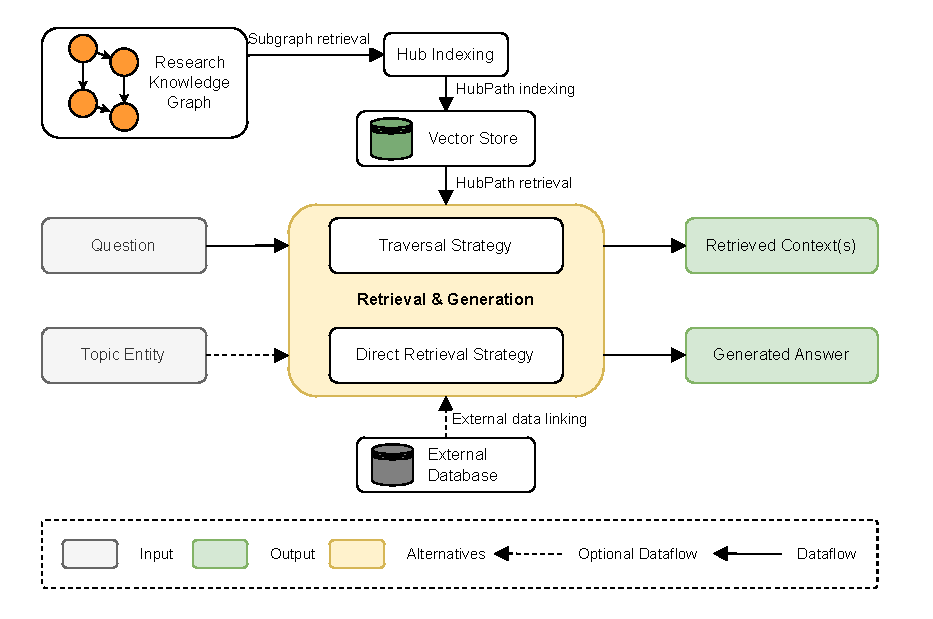
\includegraphics[width=0.95\linewidth]{figures/hublink/Hublink_figures-high_level.drawio.pdf}
%     \caption{High Level Overview of the Dataflow in HubLink}
%     \label{fig:hublink_high_level_overview}
% \end{figure}

% The dataflow of the HubLink retriever is shown in \autoref{fig:hublink_high_level_overview}. The first step of the retriever is the indexing process in which subgraphs are retrieved from an \gls{rkg}. The subgraphs consist of paths which in turn consist of triples. In the HubLink retriever, a subgraph is converted to so called \emph{HubPaths} which are stored in objects referred to as \emph{Hubs}. These are then stored in a vector store in form of low-dimensional vectors. The detailed indexing process is explained in 

This section provides an overview of our proposed HubLink approach. The purpose of this section is to illustrate the overall processes involved before diving deeper into the details in subsequent sections.

HubLink is fundamentally a \gls{grag} technique, which is characterized by its three graph-based stages: indexing, retrieval, and generation. In the following, Section~\ref{sec:hublink_indexing_process_overview} begins with the indexing process, a required preprocessing step that needs to be performed before retrieval to decompose the graph into subgraph structures referred to as \emph{hubs}. After indexing, the retrieval and generation process will be presented in Section~\ref{sec:hublink_overview_retrieval_generation}. Here, the HubLink retriever utilizes one of two different strategies to retrieve relevant data from the index. 

\subsection{Indexing}
\label{sec:hublink_indexing_process_overview}

\begin{figure}[t]
    \centering
    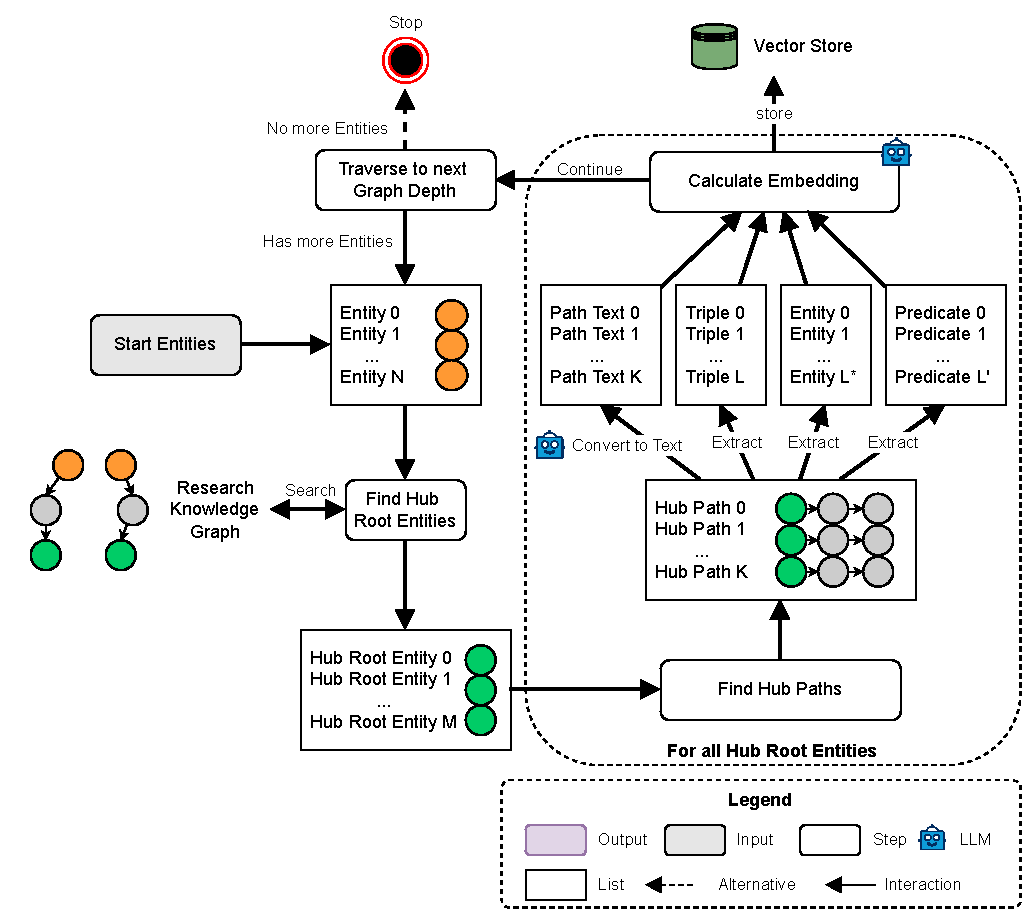
\includegraphics[width=0.93\textwidth]{figures/hublink/Hublink_figures-Overview_indexing.drawio.pdf}
    \caption[Overview of the Indexing Process]{An overview of the indexing process of HubLink showcasing how data is extracted from the \gls{kg} and stored in a vector store.}
    \label{fig:hublink_overview_indexing}
\end{figure}

The indexing process is illustrated in \autoref{fig:hublink_overview_indexing}. It begins with a set of start entities from the graph that serve as initial points for indexing. Using these entities, a search is performed with the goal of finding root entities of hubs. These are specific entities in the graph from which each hub is built. To find these roots, each possible path is traversed until either the end of the graph or until an entity in the graph is reached that is classified as the root of a hub. These identified entities are referred to as \texttt{HubRoot} objects, which are stored in a list to be processed sequentially.

For each identified \texttt{HubRoot} entity, the algorithm continues by finding and building the so-called \texttt{HubPaths}. These paths start from the \texttt{HubRoot} entity and lead to the end entities of a hub, which are either leaf nodes in the graph or other entities classified as roots of a hub. Both \texttt{HubPaths} and \texttt{HubRoot} form a \texttt{Hub} structure, which act as the central elements during retrieval.

Once the \texttt{HubPaths} of a hub are found, each path undergoes further processing before it can be indexed. First, the entire path is passed to an \gls{llm} to create a textual description of the path. In addition, an extraction of the triples, entities, and predicates from the path is performed. These pieces of information, the textual description, the triples, the entities, and the predicates, are then mapped into a low-dimensional vector space using a pre-trained embedding model. After this transformation, these vectors are stored in a vector store, which enables \gls{ann} search for fast access during the later retrieval stage. Furthermore, additional metadata are attached to each vector. This includes the root identifier of the hub for the identification of the hub to which the vector belongs and the description of the path that was generated previously by an \gls{llm}. This metadata is later required for the retrieval phase of the algorithm.

Once these hubs are indexed, the procedure repeats from the nodes in the graph that form the endpoints of each \texttt{HubPath}, provided they have not yet reached a leaf node. The indexing process stops until either the maximum number of traversal levels is reached or no new hubs are found. When the graph is updated, this update needs to be reflected in the index, which we discuss in Section~\ref{sec:updating_the_index}.

\subsection{Retrieval and Generation}
\label{sec:hublink_overview_retrieval_generation}

\begin{figure}
    \centering
    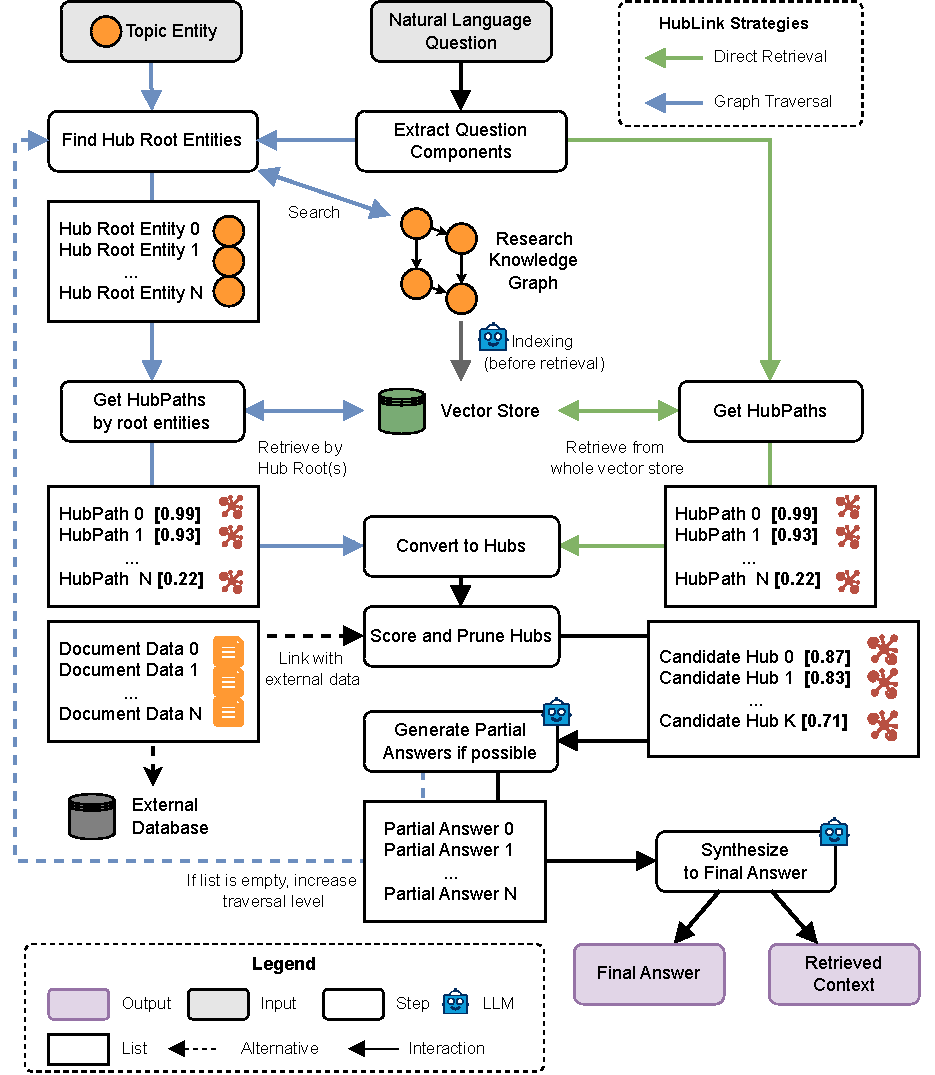
\includegraphics[width=0.98\textwidth]{figures/hublink/Hublink_figures-Overview_topic_strat.drawio.pdf}
    \caption[Overview of the Retrieval and Generation Process]{Overview of the retrieval and generation process: Two alternative strategies are depicted. The process of the direct retrieval strategy is shown with green arrows, while the graph traversal retrieval strategy is highlighted in blue.}
    \label{fig:hublink_retrieval_overview}
\end{figure}

The HubLink retrieval and generation process is illustrated in \autoref{fig:hublink_retrieval_overview}. The retriever offers two strategies for extracting relevant contexts from the \gls{kg}. The first strategy, \emph{Direct Retrieval}, performs a global search on the whole index without requiring access to the graph during retrieval. The second strategy, named \emph{Graph Traversal Retrieval}, performs a subgraph search that begins at a chosen entry point to explore the graph for the identification of relevant hubs to generate answers. The selection of the strategy involves balancing runtime and accuracy, a topic discussed later in this chapter. Both strategies differ only in certain parts of the retrieval algorithm, which we highlight in \autoref{fig:hublink_retrieval_overview} by distinguishing the paths with different colors.

The retrieval begins with an extraction of components from the question. Here, an \gls{llm} is queried to extract the most relevant parts of the question as a list. This list of components and the question itself are then transformed into vectors using the same pre-trained embedding model used in the indexing phase. Now, depending on the strategy applied, the following steps differ:

\paragraph{Graph Traversal Strategy:} In addition to the question itself, this strategy requires as input a point of entry into the graph that is referred to as \emph{Topic Entity}. The algorithm explores all paths starting at the topic entity to find \texttt{HubRoot} entities. After collecting these entities, an \gls{ann} search is performed on the vector store for each collected root entity to find \texttt{HubPaths} that are relevant to the question and contain the root entity in their metadata. This process also involves a deduplication of the paths and the application of a diversity ranker to arrive at the paths that are considered relevant to the question.

\paragraph{Direct Retrieval Strategy:} Unlike the graph traversal strategy, the direct strategy does not require a topic entity for retrieval. Furthermore, during query time, this strategy does not impose any additional queries on the graph itself. Therefore, once the components are extracted from the question, the \gls{ann} search on the vector store is directly started, which involves querying the whole store instead of querying the hubs directly, as done by the traversal strategy. Before the strategy arrives at the final \texttt{HubPaths}, it includes further techniques like clustering by hubs, deduplication of paths, and the application of a diversity ranker. 

The result of both strategies up until this point is a list of hubs with \(n\) \texttt{HubPaths} that the algorithm considers to be the most relevant to answer the question. The next step is to prune the hubs. This is done by aggregating the scores of the paths in each hub by calculating a weighted average. Only the top \(k\) hubs with the highest score are kept for the subsequent steps. 

In the next step, the \emph{Linking} process of the retriever begins. During this process, additional information is searched in an external database using the identifier of the hub, which further enriches the context of the hub beyond the knowledge collected from the graph. This could be, for example, text passages from the source publications.

By now, all necessary information about each hub has been collected. Next, for each hub, a \emph{partial answer} is generated based on the aggregated information from the hub. This is done by passing the information from the hub together with the original question in a prompt to an \gls{llm}. The \gls{llm} first checks if it is possible to provide a partial answer to the question based on this information and then provides the partial answer. If the list of partial answers is empty, no answer could be found for the question. At this step, the traversal strategy continues by traversing deeper into the graph. However, for the direct retrieval strategy, the process ends.

If partial answers have been generated, they are consolidated into a final answer. This is done by passing the partial answers to the \gls{llm} along with the original question. The \gls{llm} then generates the final answer based on this information. 


\section{Formal Definitions}
\label{sec:hublink_formal_definitions}

This section lays the formal foundation for the HubLink approach by providing definitions for the key concepts and data structures used throughout the approach. In the following, we first describe the underlying graph model to which the approach is applied. Then, we formally characterize the core elements specific to HubLink: \texttt{EntityWithDirection}, \texttt{HubRoot}, \texttt{HubPath}, \texttt{Hub}, and \texttt{HubVector}. These definitions are the prerequisites for the detailed algorithmic explanation in the following sections.

\subsection{Research Knowledge Graph (RKG)}

The underlying knowledge base is a \acrfull{rkg}, which is represented according to the \gls{rdf} standard \cite{wood_rdf_2014}. An \gls{rdf} graph provides a machine-readable semantic framework for describing ontologies, where information is expressed in the form of triples. The graph stores scholarly data where the triples capture not only bibliographic metadata (e.g., authors, dates, publishers) but also detailed relationships between scientific artifacts, for example, contributions of authors or publications. The formal definition of such an \gls{rdf} graph is provided in Section~\ref{sec:fundamentals_knowledge_graphs} and will not be repeated here.


\subsection{EntityWithDirection: Directed Graph Node}

An entity \( e \in E \) represents a node in the \gls{rdf} graph \( G \), where \( E \) is the set of all entities in the graph. Formally, the set of entities is defined as:
\[
E = \{ e \mid (s, p, o) \in G,\ e \in \{s, o\} \}.
\]

We define a path \( \mathcal{T} \) as a sequence of \( n \) triples, \( \mathcal{T} = [t_1, t_2, \ldots, t_n] \) where \( n \ge 1 \) and \( t_i = (s_i, p_i, o_i) \in G \) for all \( 1 \le i \le n \). This sequence represents a directed traversal through the graph \( G \), where adjacent triples are connected via shared entities.

When traversing such a path \( \mathcal{T} \), arriving at an entity \( e \) via the final triple \( t_n = (s_n, p_n, o_n) \) requires understanding the context: specifically, the path taken and whether \( e \) served as the subject or object. To capture this context, we introduce the \texttt{EntityWithDirection} structure. This structure associates an entity \( e \) with the specific path \( \mathcal{T} \) that ends at the entity, along with a direction indicator specifying the role of \( e \) in the final triple \( t_n \). 

Formally, we define an \texttt{EntityWithDirection} instance as a tuple \( (e, \text{dir}, \mathcal{T}) \). This tuple is constructed from a path \( \mathcal{T} = [t_1, \ldots, t_n] \), which terminates with the triple \( t_n = (s_n, p_n, o_n) \). The components \( e \) and \( \text{dir} \) are determined as follows:
\[
(e, \text{dir}) =
\begin{cases}
(s_n, \rightarrow) & \text{if the path reaches } s_n \text{ as the terminal entity} \\
(o_n, \leftarrow) & \text{if the path reaches } o_n \text{ as the terminal entity}
\end{cases}
\]
Here, \( \rightarrow \) indicates that the entity \( e \) is reached as the subject of the final triple, while \( \leftarrow \) signifies that the entity \( e \) is reached as the object.

We can now define the set \( \mathcal{D}_e \) for any given entity \( e \in E \), which includes all possible instances of \texttt{EntityWithDirection} instances that terminate at this specific entity \( e \):
\[
\mathcal{D}_e = \Big\{ (e, \text{dir}, \mathcal{T}) \;\Big|\;
\mathcal{T} = [t_1, \ldots, t_n], 
t_n = (s_n, p_n, o_n), 
(\text{dir} = \rightarrow \land e = s_n) \lor (\text{dir} = \leftarrow \land e = o_n)
\Big\}
\]

\subsection{HubRoot: Main Entity of a Hub}
\label{sec:hublink_hubroot_definition}

A \texttt{HubRoot} is an entity of the underlying \gls{rkg} and serves as the root entity of a hub. These are important for the construction of hubs, as each hub is built by collecting the paths starting from the root entity.

We denote the set of all \texttt{HubRoot} entities by \(R \subseteq V\), where \(V\) is the set of all entities in the graph \(G\). We formally define that the set of all hub roots is given by:
\[
R = \{\, v \in V \mid \phi(v) = 1 \,\},
\]
where $\phi(v)$ is a binary function to classify an entity as a \emph{HubRoot} if the criteria apply. Formally:
\[
\phi(v)=
\begin{cases}
1, & \text{if } v \text{ satisfies the hub root criteria}, \\
0, & \text{otherwise},
\end{cases}
\]

Whether \(v \in V\) is a member of \(R\) is determined by \(\phi(v)\). The criteria for defining hub roots can be based on various factors. In the following, we introduce some possibilities:

\begin{itemize}
    \item \textbf{Type-based:} The entity \(v\) has a specific type in \(G\). This is useful when the types of entities that are relevant for the \gls{qa} setting are known prior. For example, in the literature research setting, the objects of interest are publications. In this case, it is straightforward to define publications as hub types. 
    \item \textbf{Degree-based:} The degree of the outgoing edges of \(v\) exceeds a predefined threshold. This is useful when the information in a graph is highly diverse, making it difficult to define all possible types of hubs.
    \item \textbf{Path-based:} The number of paths at which \(v\) acts as the root where the paths reach a certain depth. 
    \item \textbf{Semantic-based:} The neighbors of \(v\) are checked for semantic similarity. If the similarity exceeds a predefined threshold, \(v\) is considered a root of the hub.
\end{itemize}

Defining the criteria for the hub roots is an ongoing process. We recommend choosing a hybrid approach from the methods suggested above and continually checking the coverage of the graph during indexing. It must be ensured that all entities relevant to the respective \gls{qa} setting are captured within a hub, as otherwise they cannot be fetched during the retrieval.


\subsection{HubPath: Path within a Hub}

A \texttt{HubPath} $h_r$ is built from the paths that start at a \texttt{HubRoot} $r \in R$ and lead to an end node. Each \texttt{HubPath} consists of a hash value, a textual description, and a list of \gls{rdf} triples. The hash value is used to uniquely identify the path and is generated by applying a hash function to the list of triples. The textual description is generated by an \gls{llm} and constitutes a natural language representation of $h_r$. The list of \gls{rdf} triples represents the path itself and is constructed by traversing the graph starting from the \texttt{HubRoot} entity, following the directed nature of the \gls{rdf} graph, to an end entity. 

Formally, let \(K \in \mathbb{N}\) be a predetermined maximum path length. The triple path of the \texttt{HubPath} $h_{r,i}$ is defined as a sequence
\[
\mathcal{T}_{h_{r,i}} = \langle t_1, t_2, \dots, t_k \rangle, \quad 1 \le k \le K,
\]
where each element \(t_j\) is an \gls{rdf} triple
\[
t_j = \bigl( v_{j-1}, p_j, v_j \bigr) \in G,
\]
with the convention that the initial entity \(v_0 = r\). In this context, \(v_{j-1}\) and \(v_j\) are entities, and \(p_j \in \mathcal{I}\) is the predicate. 

The following conditions are imposed on \(\mathcal{T}_{h_{r,i}}\):
\begin{enumerate}
  \item \textbf{Acyclic:} The set of entities \(\{v_0, v_1, \dots, v_k\}\) that are included in the path is required to be pairwise distinct. 
  \item \textbf{Single Outbound Degree:} Each intermediate entity \(v_j\) (for \(1 \le j < k\)) appears exactly once as the object of a triple and exactly once as the subject of a triple.
  \item \textbf{Termination:} The path terminates when at least one of the following conditions hold:
  \begin{enumerate}
    \item \emph{End of Graph:} The current entity \(v_k\) has no outgoing \gls{rdf} triple in \(G\).
    \item \emph{New Hub Root:} The current entity \(v_k\) is itself a hub root (i.e., \(v_k \in R\)).
    \item \emph{Maximum Length:} The path has reached the predetermined maximum length, \(k = K\).
  \end{enumerate}
\end{enumerate}

To preserve semantic continuity, it is important to monitor the length of the triple paths. If the paths are too long, the information from a hub might be too diverse and not semantically connected. If this is the case, reducing the maximum length of the paths can help. An alternative strategy is to adapt the definition of the \texttt{HubRoots}, which introduces more hubs and thus can also shorten the overall lengths of the \texttt{HubPaths}. However, if the paths are becoming too short, the information might not be detailed enough to answer a question. Therefore, it is important to monitor the lengths of the paths in the graph when building the index.

\begin{figure}[t]
    \centering
    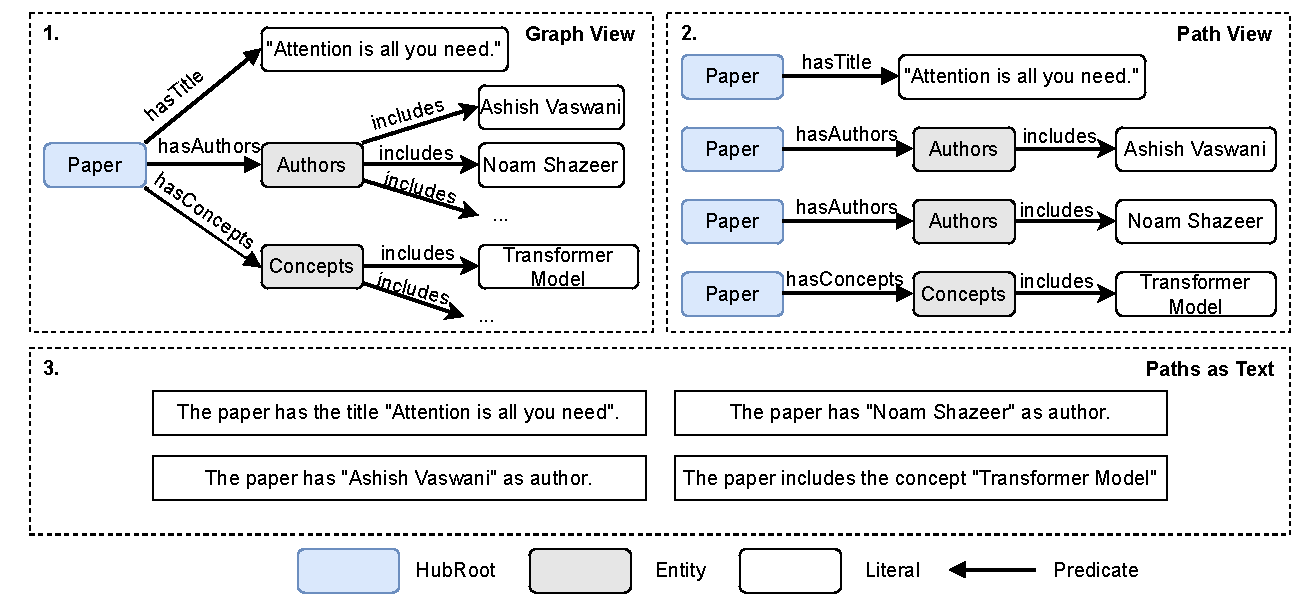
\includegraphics[width=1.0\linewidth]{figures/hublink/Hublink_figures-build_hubs.drawio.pdf}
    \caption[Path to Text Conversion]{Conversion of paths consisting of triples to textual descriptions using an \gls{llm}.}
    \label{fig:path_to_text_conversion}
\end{figure}

With the triple path $\mathcal{T}_{h_{r,i}}$, we can now define the hash value of the \texttt{HubPath} \(h_{r,i}\) as
\[
\phi_{r,i} = \text{hash}(\mathcal{T}_{h_{r,i}}) \in \mathcal{B},
\]
where \(\mathcal{B}\) is the set of all possible hash values. The hash value is generated by applying a hash function to the list of triples in the path. This will produce a unique value for each unique path, ensuring that no two paths have the same hash value, provided that the hash function is free from collisions. We then obtain the textual description of the \texttt{HubPath} \(h_{r,i}\) by applying a function:
\[
T_{\text{path}}: \mathcal{T}_{h_{r,i}} \to \mathcal{X},
\]
This function takes a triple path as input and outputs a textual description in a space \(\mathcal{X}\) of natural language strings. In \autoref{fig:path_to_text_conversion}, this process is illustrated. It shows the initial graph view and the decomposition of the hub subgraph into individual triple paths. These are then converted into a textual representation using the function \(T_{\text{path}}\) which is realized by an \gls{llm} that processes the sequence of \gls{rdf} triples $\mathcal{T}_{h_{r,i}}$ and generates a natural language description.

The final \texttt{HubPath} \(h_{r,i}\) is then defined as a tuple
\[
h_{r,i} = \bigl( \phi_{r,i}, T_{\text{path}}(\mathcal{T}_{h_{r,i}}), \mathcal{T}_{h_{r,i}} \bigr),
\]
where \(\phi_{r,i}\) is the hash value, \(T_{\text{path}}(\mathcal{T}_{h_{r,i}})\) is the textual description, and \(\mathcal{T}_{h_{r,i}}\) is the list of triples. The \texttt{HubPath} \(h_{r,i}\) is thus a representation of the path information inside a hub. This leads us to define the set of all \texttt{HubPaths} starting from the root of the hub \(r\). Formally, let \(r \in R\) be the root of the hub, where \(R\) is the set of \texttt{HubRoots} as defined in the previous section. 
We define the set of all HubPaths starting at \(r\) as
\[
\mathcal{H}(r) = \{\, h_r \mid h_r \text{ is a HubPath starting at } r \,\}.
\]

\subsection{Hub: Aggregation of Semantically Related Information}

A \texttt{Hub} is a special construct in the HubLink retriever that is used to aggregate semantically related information about a specific knowledge entity. It always consists of a \texttt{HubRoot} entity and a set of \texttt{HubPaths}. Formally, a hub is defined as
\[
Hub_r = \bigl( r,\, \mathcal{H}(r) \bigr),
\]
where \(r \in R\) is a hub root and \(\mathcal{H}(r)\) is the collection of hub paths starting from \(r\).

\subsection{HubVector: Encoding of Hub Information}
\label{sec:hublink_hubvector_definition}

To be able to efficiently retrieve relevant information from a hub, the \texttt{HubPaths} of the hub are encoded in a vector space using \texttt{HubVectors}. A \texttt{HubVector} is a low-dimensional vector representation constructed from the information of a \texttt{HubPath} and is always stored together with additional metadata that includes the hub root identifier \(r \in R\) and the textual description $T_{\text{path}}(\mathcal{T}_{h_{r,i}})$ of the \texttt{HubPath}. The goal is to project the semantic content of each \texttt{HubPath} into a vector space using a pre-trained embedding model, where a nearest-neighbor search such as \gls{ann} can be performed. What is important to consider here is that the path itself may contain too much information, which can lead to a phenomenon where the relevant information is obscured by the complexity of the path. To reduce this risk, the path is decomposed into different parts, increasing the likelihood of a nearest-neighbor search to find relevant information. More information on this design decision is provided in Section~\ref{sec:hublink_design_rationale}. 

By decomposing the \texttt{HubPath}, we define four vector representations. Let \(h_{r,i}\) denote the \(i\)-th \texttt{HubPath} of the hub with root \(r\). We define a general embedding function
\[
f: \mathcal{X} \to \mathbb{R}^d,
\]
which maps any textual input into a \(d\)-dimensional vector. We distinguish four types of \texttt{HubVectors} that can be generated from a hub path \(h_{r,i}\):

\begin{itemize}
    \item \textbf{Path Vector:} This vector represents the overall semantic content of the \texttt{HubPath}. It is obtained by embedding the full natural language description $T_{\text{path}}(\mathcal{T}_{h_{r,i}})$ of the path $\mathcal{T}_{h_{r,i}}$ generated by the \gls{llm}:
    \[
    \mathbf{v}_{\text{path}}(h_{r,i}) = f\Bigl( T_{\text{path}}(\mathcal{T}_{h_{r,i}}) \Bigr) \in \mathbb{R}^d
    \]
    
    \item \textbf{Triple Vector:} For this vector type, the triple path $\mathcal{T}_{h_{r,i}}$ is broken down into its individual triples. Each triple \(t_k \in \mathcal{T}_{h_{r,i}}\) is converted into a vector representation:
    \[
    \mathcal{V}_{\text{triples}} = \{f (t_k) \mid t_k \in \mathcal{T}_{h_{r,i}}\}, \quad f(t_k) \in \mathbb{R}^d
    \]
    
    \item \textbf{Entity Vector:} For this vector type, the triple path $\mathcal{T}_{h_{r,i}}$ is decomposed into all entities contained in the path. For each triple \(t_k = (s,p,o) \in \mathcal{T}_{h_{r,i}}\) , the entities \(s\) and \(o\) are extracted. Each entity is then embedded using \(f\):
    \[
    \mathcal{V}_{\text{entities}} = \{f(e) \mid t_k = (s, p, o) \in \mathcal{T}_{h_{r,i}},\ e \in \{s, o\}\}, \quad f(e) \in \mathbb{R}^d
    \]

    \item \textbf{Predicate Vector:} For this vector type, the hub path \(h_{r,i}\) is decomposed into all predicates contained in the path. For each triple \(t_k = (s,p,o) \in \mathcal{T}_{h_{r,i}}\), the predicate $p$ is extracted and embedded using \(f\). The embedding for each predicate is then computed as:
    \[
    \mathcal{V}_{\text{predicates}} = \{f(p) \mid t_k = (s, p, o) \in \mathcal{T}_{h_{r,i}}\}, \quad f(p) \in \mathbb{R}^d
    \]
\end{itemize}

For each hub path \(h_{r,i}\), multiple \texttt{HubVectors} are thus stored in the vector store. Each vector is stored as a tuple containing the root of the hub \(r\), the natural language description \(T_{\text{path}}(\mathcal{T}_{h_{r,i}})\), and the corresponding vector representation. Formally, we define the set of all \texttt{HubVectors} for \(h_{r,i}\) as:
\[
\begin{aligned}
    \mathcal{V}(h_{r,i}) =\;
    & \Bigl\{ \bigl( r,\; T_{\text{path}}(\mathcal{T}_{h_{r,i}}),\; \mathbf{v}_{\text{path}}(h_{r,i}) \bigr) \Bigr\} \\
    & \cup \Bigl\{ \bigl( r,\; T_{\text{path}}(\mathcal{T}_{h_{r,i}}),\; v \bigr) \mid v \in \mathcal{V}_{\text{triples}} \Bigr\} \\
    & \cup \Bigl\{ \bigl( r,\; T_{\text{path}}(\mathcal{T}_{h_{r,i}}),\; v \bigr) \mid v \in \mathcal{V}_{\text{entities}} \Bigr\} \\
    & \cup \Bigl\{ \bigl( r,\; T_{\text{path}}(\mathcal{T}_{h_{r,i}}),\; v \bigr) \mid v \in \mathcal{V}_{\text{predicates}} \Bigr\} \\
\end{aligned}
\]

Note that each vector is stored alongside the textual path description \(T_{\text{path}}(\mathcal{T}_{h_{r,i}})\) because decomposing the path into individual triples, entities, or predicates results in a loss of the semantic relationships between nodes. This can lead to reduced retrieval performance when a query matches a triple, entity, or predicate, as the isolated vector may not capture enough context to represent the full meaning. To address this, the textual description of the path \(T_{\text{path}}(\mathcal{T}_{h_{r,i}})\) is stored as metadata within each vector tuple. While the vector is used for similarity-based retrieval, the associated textual description is used during answer generation.

Finally, given a hub \(Hub_r = (r, \mathcal{H}(r))\), the overall set of \texttt{HubVectors} for the hub is defined as:
\[
\mathcal{V}(Hub_r) = \bigcup_{h \in \mathcal{H}(r)} \mathcal{V}(h).
\]
This collection of vectors, together with their associated metadata, forms the basis for the retrieval process in HubLink.



\section{Data Models}
\label{sec:hublink_data_models}

\begin{figure}
\begin{algorithmic}[1]

\Statex \textbf{Class:} \texttt{Entity} \(\leftarrow e\in E\) \Comment{Represents a node \(e\) in the graph}
    \Statex \quad ID: \texttt{String}
    \Statex \quad Value: \texttt{String}
\Statex \textbf{Class:} \texttt{Triple} \(\leftarrow  t = (s, p, o) \in G\) \Comment{Represents a triple in the graph}
    \Statex \quad Subject: \texttt{Entity}
    \Statex \quad Predicate: \texttt{String}
    \Statex \quad Object: \texttt{Entity}

\Statex
\Statex \textbf{Class:} \texttt{EntityWithDirection} \(\leftarrow (e, \text{dir}, \pi) \in \mathcal{D}_e\)
    \Statex \quad Entity: \texttt{Entity} \Comment{An entity in the graph}
    \Statex \quad Direction: \texttt{Enum} \Comment{Indicates if the entity is subject or object in the current path}
    \Statex \quad PathToEntity: \texttt{List} of \texttt{Triple} \Comment{The directed triple path leading to the entity}

\Statex
\Statex \textbf{Class:} \texttt{Hub} \(\leftarrow Hub_r = (r, \mathcal{H}(r))\)
    \Statex \quad Root: \texttt{EntityWithDirection} \Comment{The root node \(r\) of the hub}
    \Statex \quad Paths: \texttt{List} of \texttt{HubPath} \Comment{All paths in the hub rooted at \(r\)}
    \Statex \quad Score: \texttt{Float} \Comment{Combined score for all paths}

\Statex
\Statex \textbf{Class:} \texttt{HubPath} \(\leftarrow h_{r,i} \in \mathcal{H}(r)\)
    \Statex \quad PathText: \texttt{String} \Comment{Textual description of the path}
    \Statex \quad PathHash: \texttt{String} \Comment{Unique hash of the path}
    \Statex \quad Path: \texttt{List} of \texttt{Triple} \Comment{Sequence of triples representing the path}
    \Statex \quad EmbeddedText: \texttt{String} \Comment{The text used to create the embedding}
    \Statex \quad Score: \texttt{Float} \Comment{Relevance score toward the query}

\Statex
\Statex \textbf{Class:} \texttt{ProcessedQuestion}
    \Statex \quad Question: \texttt{String} \Comment{The original question that is asked}
    \Statex \quad Components: \texttt{List} of \texttt{String} \Comment{Components of the original question}
    \Statex \quad Embeddings: \texttt{List} of \texttt{List} of \texttt{Float} \Comment{Embeddings of components and question}

\Statex
\Statex \textbf{Class:} \texttt{LinkData}
    \Statex \quad HubIdentifier: \texttt{String} \Comment{Identifier associated with the data}
    \Statex \quad Text: \texttt{String} \Comment{Additional data to enrich the hub}

\end{algorithmic}
\caption[Data Models with Formal Definitions]{The data models used by HubLink mapped to their formal definitions (Data model $\leftarrow$ Formal definition).}
\label{alg:data_models}
\end{figure}


The data models used in the \textsc{HubLink} retriever are shown in \autoref{alg:data_models}. Each class corresponds to a formal element defined in Section~\ref{sec:hublink_formal_definitions}, with the mapping expressed using the notation \(\textsc{Class} \leftarrow \textsc{Formal Definition}\). In the following, we provide a description of each data model:

\paragraph{Entity} The entity data model represents a node in the graph. Each entity is associated with an identifier that uniquely identifies the entity in the graph, is associated with a value, and may also have a type. Depending on the graph, this type can be either stored directly with the entity or described using an edge to the entity. For HubLink, it is not necessary that an entity has a type, but it is advantageous for the classification of hubs.

\paragraph{Triple} The triple data model conforms to the \gls{rdf} definition. As such, it contains a subject and an object, which are both \texttt{Entity} types. The predicate describes their relation and is a \texttt{String}.

\paragraph{EntityWithDirection} This data model stores a direction and a path to an entity. Consequently, it acts as a wrapper for an \texttt{Entity} in the HubLink algorithm. 

\paragraph{Hub} The data model for a hub includes a root, which is an \texttt{EntityWithDirection} object. This root acts as a unique identifier for the hub itself and is used for building the \texttt{HubPath} objects. In addition, each hub has a score that is calculated during the retrieval to assess the relevance of the hub to the question that is asked.

\paragraph{HubPath} The data model for the \texttt{HubPath} stores the unique hash value that acts as an identifier for the \texttt{HubPath}. The textual description and the associated triple path are also stored. In addition, the model stores the text by which the path has been retrieved from the vector store. This is required as each \texttt{HubPath} is stored at different levels (path, triple, entity, or predicate level). Finally, the score that assesses the relevance of the \texttt{HubPath} to the question asked is saved in the data model.

\paragraph{ProcessedQuestion} This data model is used to store the question that is asked to the retriever, the components that have been extracted from the question, and the precomputed embeddings for both the question and the components.

\paragraph{LinkData} This data model is created during the linking process. It stores the identifier of the hub to which it is associated and a text. The text is additional information collected from an external database that is relevant to enrich the retrieval data for comprehensive answer generation.


\section{Finding Hub Root Entities}
\label{sec:hublink_finding_hub_root_entities}

\begin{algorithm}
\caption{Pseudocode for Finding Hub Root Entities}
% \caption[Pseudocode for Finding Hub Roots]{Pseudocode for finding the \texttt{HubRoot} entities of a hub. The search is performed by applying a breadth-first search where for each entity that is reached a classification takes place to classify whether this entity is qualified to be a \texttt{HubRoot}.}
\label{alg:finding_hub_roots}
\begin{algorithmic}[1]
\PersistentState
    \Statex $visited$: \texttt{Set} of \texttt{EntityWithDirection} \Comment{List of visited entities}
    \Statex $G$: \texttt{KnowledgeGraph} \Comment{The graph to search in}
\Require 
    \Statex $\vec{E}$: \texttt{List} of \texttt{EntityWithDirection} \Comment{Entities to start the search from}
    \Statex \texttt{UniformHopCount}: \texttt{Boolean} \Comment{Require uniform hop count when reaching the hubs}
\Ensure
    \Statex A tuple $(\texttt{hub\_entities}, \texttt{next\_entities})$ containing the entities that are the root of a Hub and the entities that are used to initialize the search on the next level.
\Statex
\Function{findHubRoots}{$\vec{E}, \texttt{UniformHopCount}$} 
    \State Initialize $queue \gets$ \texttt{Queue}($\vec{E}$)
    \State $hub\_roots \gets \emptyset$ \Comment{Collection of Hub root entities found}
    \State $next\_entities \gets \emptyset$ \Comment{Candidates returned for the next depth}
    
    \While{$queue \neq \emptyset$}
        \State $e \gets$ \Call{dequeue}{$queue$} \Comment{Current entity to process}
        \State \textbf{if} $e \in visited$ \textbf{then Continue}
        \State $visited \gets visited \cup \{e\}$ 
        \State $e_{\text{isHubRoot}} \gets$ \Call{isHubRoot}{$e$} \Comment{Check if entity is a hub}
        
        \If{$e_{\text{isHubRoot}}$ \textbf{and} $e \notin \text{hub\_roots}$}
            \State $hub\_roots \gets hub\_roots \cup \{e\}$
        \EndIf
        
        \If{$e_{\text{isHubRoot}}$ \textbf{and} $\neg e.\text{Left}$}
            \State \textbf{Continue} \Comment{Stop traversing the current path}
        \EndIf
        
        \State $entity\_triples \gets \{\text{All adjacent triples of } e \text{ considering its direction}\}$
        
        \If{not \texttt{UniformHopCount}}
            \State enqueue all $entity\_triples$ into $queue$
        \Else
            \State $next\_entities \gets next\_entities \cup entity\_triples$
        \EndIf
    \EndWhile
    
    \State \Return $(hub\_roots, next\_entities)$
\EndFunction

\end{algorithmic}
\end{algorithm}

The function \textsc{findHubRoots}, shown in \autoref{alg:finding_hub_roots}, is responsible for identifying the \texttt{HubRoot} entities of hubs starting from a list of input entities \(\vec{E}\), which serve as the initial traversal points within the graph \(G\). The function follows a breadth-first search strategy, meaning that all neighboring entities are explored before descending to a deeper level. To begin the search, a queue is initialized with \(\vec{E}\). Then, a loop is performed that terminates once the queue is empty. In each iteration, one entity \(e\) is dequeued and processed. If \(e\) has already been visited (as tracked in the \texttt{visited} set), it is skipped. Otherwise, it is marked as visited, and the function \texttt{isHubRoot} is called to determine whether the entity can be classified as a \texttt{HubRoot}. If \(e\) is identified as a \texttt{HubRoot} and has not already been added, it is added to the set \(hub\_roots\) to be returned once the search has finished. Next, a determination for the continuation of the search is performed. If \(e\) is a \texttt{HubRoot} and its traversal direction is \texttt{Right}, the search along that path is terminated, and the algorithm proceeds to the next entity. This is because the \texttt{HubPaths} of a hub are built following this direction, which means that those paths will be collected later during the building of the hubs. For all other cases, the function collects the triples in which \(e\) participates. These are either queued for further traversal or stored in the set \(next\_entities\), depending on the parameter \texttt{UniformHopCount}. The loop continues until the queue is empty. Once the loop ends, the function returns two sets: \(hub\_roots\), which contains the discovered hub entities, and \(next\_entities\), which are passed to the next level of traversal in the indexing process.

\begin{tcolorbox}[title=Parameter: \texttt{UniformHopCount}]
This parameter determines whether the traversal should continue beyond the first iteration and is only relevant for the \emph{graph traversal} retrieval strategy. If \(\texttt{UniformHopCount} = \texttt{False}\), all \texttt{HubRoots} directly reachable from the current entities in \(\vec{E}\) are considered. Otherwise, the traversal continues recursively until a \texttt{HubRoot} is found. This is useful when \texttt{HubRoots} lie at varying depths in the graph and a uniform number of hops to reach the entity cannot be assumed. Therefore, it should be chosen whether to set \texttt{UniformHopCount} or not based on the structure of the graph.
\end{tcolorbox}

\begin{tcolorbox}[title=Persistent State: \(\texttt{visited}\)]
The \texttt{visited} set keeps track of entities that have already been processed, taking the direction into account. This ensures that nodes are not revisited multiple times and that cycles in the graph do not cause infinite loops. Notably, this set is persistent for subsequent calls to ensure that cycles are handled for the same retrieval or indexing. Consequently, this persistent state must be cleared once the retrieval or indexing is complete, which can be accomplished by implementing the function in a class and initializing the class for each new retrieval or indexing.
\end{tcolorbox}

\begin{tcolorbox}[title=Function: \textsc{isHubRoot}]
Whether an entity is classified as a hub is determined by the \textsc{isHubRoot} function. There are several ways to do this classification, as described in Section~\ref{sec:hublink_formal_definitions}. The easiest way is to define a list of types that should be classified as a hub and check if the given entity is of that type.
\end{tcolorbox}




\section{Indexing}
\label{sec:hublink_indexing}

%%%% Algorithm for Indexing Hubs

The pseudocode for the indexing process is shown in \autoref{alg:indexing_hubs}. As input, the function requires a list of starting entities \(\vec{E}\) and the parameter \texttt{MaxIndexingDepth}, which controls how deep the algorithm traverses \(G\), and thus how large \(\hat{G}\) becomes, which is the indexed subgraph. This design choice is motivated by the potential size of the graph \(G\), which can contain millions of nodes. Using the starting entities \(\vec{E}\) and the maximum indexing depth \texttt{MaxIndexingDepth}, it allows to effectively choose between indexing the entire graph or only a subgraph \(\hat{G}\).

The indexing algorithm consists of a loop that terminates when one of the following conditions is met:
\begin{enumerate}
    \item \texttt{MaxIndexingDepth} is reached,
    \item the list of entities to process becomes empty, or
    \item no further nodes are found for traversal.
\end{enumerate}

In each iteration, the algorithm calls the function \textsc{findHubRoots} to identify \texttt{HubRoot} objects at the current depth, as well as a new set of entities to explore in the next iteration. Once found, the hub roots are passed to the \textsc{buildHubs} function, which builds the \texttt{Hub} objects. Then, to prepare the next iteration, the entities located at the ends of these hubs are added to the list of entities used to continue the indexing in the next iteration of the loop.

\begin{algorithm}[t]
\caption{Pseudocode for Indexing of Hubs}
% \caption[Pseudocode for Indexing]{Pseudocode for the indexing process. Starting from a specified set of entities, the graph is traversed up until a maximum depth while building \texttt{Hubs} for each \texttt{HubRoot} encountered during traversal.}
\label{alg:indexing_hubs}
\begin{algorithmic}[1]
\PersistentState
    \Statex $G$: \texttt{KnowledgeGraph} \Comment{The graph to search in}
\Require 
    \Statex $\vec{E}$: \texttt{List} of \texttt{Entity} \Comment{Entities from which the indexing is started}
    \Statex $\texttt{MaxIndexingDepth}$: \texttt{Integer} \Comment{Maximum allowed indexing depth}

\Procedure{hubIndexing}{$\vec{E}, \texttt{MaxIndexingDepth}$}
    \State $entities \gets \{ \texttt{EntityWithDirection}(T, \textbf{true}, \emptyset) \mid T \in \vec{E} \}$
    \State $entities \gets entities \cup \{ \texttt{EntityWithDirection}(T, \textbf{false}, \emptyset) \mid T \in \vec{E} \}$
    \If{$entities = \emptyset$}
        \State \Return
    \EndIf
    \State $depth \gets 0$ 
    
    \While{$depth \leq \texttt{MaxIndexingDepth}$}
        \State $hub\_roots, next\_entities \gets$ \Call{findHubRoots}{$entities$}
        \State $entities \gets next\_entities$
        \State $hub\_end\_entities \gets$ \Call{buildHubs}{$hub\_roots$}
        \State $entities \gets entities \cup hub\_end\_entities$
        \If{$entities = \emptyset$}
            \State \textbf{break} \Comment{Stop if no more entities to process}
        \EndIf
        \State $depth \gets depth + 1$
    \EndWhile
\EndProcedure
\end{algorithmic}
\end{algorithm}

\begin{tcolorbox}[title=Parameter: \texttt{MaxIndexingDepth}]
This parameter defines the maximum traversal depth at which \texttt{HubRoot} objects are located. It is important to note that this depth does not correspond to the entities of the graph themselves, but only those classified as \texttt{HubRoots}. Since building a hub involves traversing internal paths within the hub itself, the total depth of entities indexed may exceed \texttt{MaxIndexingDepth}.
\end{tcolorbox}




\subsection{Building Hubs}
\label{sec:hublink_building_hubs}

%%%% Algorithm for Building Hubs
\begin{algorithm}
\caption{Pseudocode for Building Hubs}
% \caption[Pseudocode for Building Hubs]{Pseudocode for building \texttt{Hub} objects. This involves an update check to determine, whether the hub needs to be updated or the current index is already up-to-date. The function then creates the \texttt{HubPath} objects of the hub and stores them in the vector store.}
\label{alg:building_hubs}
\begin{algorithmic}[1]
\PersistentState
    \Statex $\hat{V}$: \texttt{VectorStore} \Comment{Persistent storage for hub-related data}
\Require 
    \Statex $\vec{R}$: \texttt{List} of \texttt{Entity} \Comment{Root entities of the hubs}
\Ensure
    \Statex A list of entities that are used for the next indexing depth.

\Statex
\Function{buildHubs}{$\vec{R}$}
    \State $next\_entities \gets \emptyset$ \Comment{Entities for deeper indexing}
    \ForAll{$r \in \vec{R}$}
        \State $(\vec{p}, \vec{e}) \gets$ \Call{findPathsInHub}{$r$}
        \State $next\_entities \gets next\_entities \cup \vec{e}$
        
        \State $needs\_rebuild \gets$ \Call{hubIndexNeedsToBeUpdated}{$r, \vec{p}$}
        
        \If{$needs\_rebuild$}
            \State $hub\_paths \gets$ \Call{buildHubPaths}{$\vec{p}$}
            \State \Call{storeHubPaths}{$hub\_paths, r$}
        \EndIf
    
    \EndFor
    \State \Return $next\_entities$
\EndFunction
\end{algorithmic}
\end{algorithm}

A hub $Hub_r \bigl(r, \mathcal{H}(r) \bigr)$ consists of the root $r$ and the \texttt{HubPaths} $\mathcal{H}(r)$. Consequently, the building process is two-fold. First, the triple paths of a hub have to be extracted from the graph, and then the \texttt{HubPath} objects have to be created. Then, the paths have to be stored in the vector store.

The function for building hubs is detailed in \autoref{alg:building_hubs}. This function takes as input a list of root entities \(\vec{R}\), each of which is assumed to be confirmed \texttt{HubRoot} objects. The algorithm then iterates over every entity \(r \in \vec{R}\) to construct the corresponding hub. This is realized in a loop that processes each root entity \(r\). It calls the function \textsc{findPathsInHub} that identifies and returns all triple paths originating from \(r\) that are relevant for building the \texttt{HubPath} objects. The function further returns a set of additional entities that may serve as roots for nested hubs, which are collected in the set \(next\_entities\) for further indexing. Next, the function \textsc{hubIndexNeedsToBeUpdated} is invoked to determine whether the current hub must be created or updated. If this is the case, \textsc{buildHubPaths} is called to generate a new set of \texttt{HubPath} objects based on previously identified paths. After the paths have been collected, the \textsc{storeHubPaths} function is called, which adds them to the vector store.

\begin{tcolorbox}[title=Persistent Storage: Vector Store \(\hat{V}\)]
The vector store \(\hat{V}\) serves as persistent storage for all indexed \texttt{HubPath} objects. As mentioned in Section~\ref{sec:hublink_formal_definitions}, it stores four types of vectors on the path, triple, entity, and predicate level. During indexing, the vector store is filled with the vectors, and during retrieval, similarity matches to the vectors are performed to find those \texttt{HubPath} objects that are most relevant to the query.
\end{tcolorbox}

\subsection{Checking for Graph Updates}

\begin{algorithm}
\caption{Pseudocode for Determining Index Update}
% \caption[Pseudocode for Determining Index Update]{Pseudocode for checking whether the index of a \texttt{Hub} needs to be updated. This is done by verifying whether all \texttt{HubPaths} include the same content as the graph.}
\label{alg:hub_update_check}
\begin{algorithmic}[1]
\PersistentState
    \Statex $\hat{V}$: \texttt{VectorStore} \Comment{A vector store to store hub data}
\Require 
    \Statex $r$: \texttt{EntityWithDirection} \Comment{The root entity of the hub}
    \Statex $\vec{p}$: \texttt{List} of \texttt{List} of \texttt{Triple} \Comment{The collected paths for the hub}
\Ensure
    \Statex \texttt{Boolean} indicating whether the hub data in the vector store needs to be updated

\Statex
\Function{hubIndexNeedsToBeUpdated}{$r, \vec{p}$}
    \State $\delta \gets$ \Call{computeHashesForPaths}{$\vec{p}$}
    \State $\gamma \gets$ \Call{getStoredPathHashes}{$r$}
    \If{$\delta \neq \gamma$}
        \State \Return \textbf{true}
    \Else
        \State \Return \textbf{false}
    \EndIf
\EndFunction
\Statex
\Function{getStoredPathHashes}{$r$}
    \State $v \gets \hat{V}.\Call{getAllPathVectors}{r}$
    \State $\gamma \gets \emptyset$
    \ForAll{$vector \in v$}
        \State $h \gets vector.metadata.pathHash$
        \State $\gamma \gets \gamma \cup \{h\}$
    \EndFor
    \State \Return $\gamma$
\EndFunction
\Statex
\Function{computeHashesForPaths}{$\vec{p}$}
    \State $\delta \gets \emptyset$
    \ForAll{$p \in \vec{p}$}
        \State $\delta \gets \delta \cup \{\Call{hash}{p}\}$
    \EndFor
    \State \Return $\delta$
\EndFunction
\end{algorithmic}
\end{algorithm}

\autoref{alg:hub_update_check} provides pseudocode to verify whether the index of a hub stored in the vector store \(\hat{V}\) is still consistent with the current state of the graph. It plays a key role in ensuring that the index remains consistent with the underlying graph without unnecessarily rebuilding hubs that are already up-to-date. 

The check is performed by the function \textsc{hubIndexNeedsToBeUpdated}, which takes as input the root entity \(r\) of a hub and a list of current triple paths \(\vec{p}\). The function operates under the assumption that the paths in \(\vec{p}\) represent the latest structure of the graph. To verify consistency, it first computes a hash value for each triple path and stores the resulting set in \(\delta\) via the function \textsc{computeHashesForPaths}. These hashes serve as a signature of the current hub structure. Next, the function \textsc{getStoredPathHashes} retrieves the stored path hashes from the vector store \(\hat{V}\) for the given root entity \(r\). These are collected in the set \(\gamma\), which represents the last known indexed state of the hub. Finally, the sets \(\delta\) and \(\gamma\) are compared. If they differ, it means that the indexed hub is outdated and needs to be rebuilt. In this case, the function returns \texttt{true}. Otherwise, it returns \texttt{false}.

Using hash values to compare hub path structures offers an efficient and scalable way to detect changes without needing to perform expensive graph diffing or structural comparisons. Each triple path is mapped to a compact, fixed-size hash, which acts as a unique signature of its content. This allows the algorithm to perform fast set-based comparisons between the current state of the graph and the previously stored hub data. As long as the hash function is consistent and resistant to collision, this approach reliably identifies when any part of the path structure of a hub has changed, thus triggering a rebuild only when necessary.


\subsection{Finding the Triple Paths of a Hub}

\begin{algorithm}[p]
\caption{Pseudocode for Finding the Triple Paths of a Hub}
% \caption[Pseudocode for Finding the Hub Triple Paths]{Pseudocode for finding the paths consisting of triples with a \texttt{HubRoot} entity as the root of each path.}
\label{alg:finding_paths_in_hub}
\begin{algorithmic}[1]
\PersistentState
    \Statex $G$: \texttt{KnowledgeGraph} \Comment{The graph to search in}
\Require 
    \Statex $R$: \texttt{Entity} \Comment{Root entity of the hub}
    \Statex \texttt{MaximumPathLength}: \texttt{Integer} \Comment{Maximum allowed path length}
\Ensure
    \Statex A tuple \((paths, candidates)\), where $paths$ are the collected triple paths, and $candidates$ are entities at hub boundaries

\Statex
\Function{findPathsInHub}{$R, \texttt{MaximumPathLength}$}
    \State $visited \gets \emptyset$ \Comment{Set of entities visited}
    \State $candidates \gets \emptyset$ \Comment{Candidates for next level}
    \State $paths \gets \emptyset$ \Comment{Paths of triples from the graph}
    \State $queue \gets$ a new queue initialized with \((R, \emptyset)\)
    
    \While{$queue \neq \emptyset$}
        \State $(e, \vec{p}) \gets$ \Call{dequeue}{$queue$} \Comment{Current entity and path}
        \If{$e \in visited$ and $e \neq R$}
            \State \textbf{continue} \Comment{Avoid revisiting entities}
        \EndIf
        \State $visited \gets visited \cup \{e\}$

        \If{$|\vec{p}| \geq \texttt{MaximumPathLength}$}
            \State $paths \gets paths \cup \{\vec{p}\}$
            \State \textbf{continue}
        \EndIf
        
        \State $\vec{t} \gets$ \Call{getOutboundTriples}{$e, G$} \Comment{Retrieve all neighbors of $e$}
        \If{$\vec{t} = \emptyset$}
             \State $paths \gets paths \cup \{\vec{p}\}$ \Comment{Leaf entity of graph reached}
            \State\textbf{continue}
        \EndIf
        
        \ForAll{$triple \in \vec{t}$}
            \State $e' \gets triple.Object$
            \If{$e' = R$}
                \State \textbf{continue} \Comment{Skip cycles back to root}
            \EndIf
            \If{\Call{isHubRoot}{$e'$}}
                \State $candidates \gets candidates \cup \{e'\}$
                \State $paths \gets paths \cup \{\vec{p}\}$
            \Else
                \State $\vec{p'} \gets \vec{p} \mathbin{++} \{triple\}$ \Comment{Append triple to path}
                \State enqueue \((e', \vec{p'})\) into $queue$ \Comment{Add neighbor to queue}
            \EndIf
        \EndFor
    \EndWhile
    
    \State \Return $(paths, candidates)$
\EndFunction
\end{algorithmic}
\end{algorithm}

To find all relevant triple paths associated with a hub, the function \textsc{findPathsInHub}, shown in \autoref{alg:finding_paths_in_hub}, is used. This function is invoked with the root entity \(R\) of a hub, the knowledge graph \(G\), and the parameter \(\texttt{MaximumPathLength}\). It returns all valid triple paths starting at \(R\), together with a list of candidate entities that mark the boundary of the hub for further indexing.

At the start of the function, three sets are initialized: \texttt{visited}, \texttt{candidates}, and \texttt{paths}. The \texttt{visited} set tracks entities already explored to prevent cycles. The \texttt{candidates} set stores entities that are themselves hubs and may serve as roots for nested hubs in later indexing stages and the \texttt{paths} set contains all complete triple paths discovered within the hub.

A queue is initialized with a tuple containing the root entity \(R\) and an empty path. The function performs a breadth-first traversal using this queue. In each iteration, an entity \(e\) and its associated path \(\vec{p}\) are dequeued. If \(e\) has already been visited and is not the root, it is skipped. If the current path length has reached the maximum allowed length, the path is stored, and traversal for that branch ends. Otherwise, the function retrieves all outbound triples of \(e\). If there are no outbound triples, the node is considered a leaf, and the current path is saved. However, if there are outbound triples, each triple is examined. This is done by extracting the entity object \(e'\) from the triple. The reason we are only looking at the objects of the \gls{rdf} triples is that, by convention, the paths of a hub are only examined in the natural direction of the graph. The algorithm then continues by checking whether \(e'\) is the \texttt{HubRoot} of the hub \(R\). In this case, it is skipped to avoid cycles. If \(e'\) is identified as a \texttt{HubRoot} for another hub, it is added to the \texttt{candidates} set, and the current path is stored without traversing further in that direction. Otherwise, the triple is appended to the current path and the new state \((e', \vec{p}')\) is enqueued for further exploration. This process continues until the queue is empty. At that point, all discovered paths and candidate hub boundaries have been collected and are returned by the function.

\begin{tcolorbox}[title=Parameter: \texttt{MaximumPathLength}]
The parameter \texttt{MaximumPathLength} limits how deeply the algorithm explores the graph from the \texttt{HubRoot} $R$. It defines the maximum allowed length of any \texttt{HubPath} and helps control the scope and relevance of each path. A path that is too long may lose semantic connection to the core context of the hub. Therefore, choosing an appropriate value for \texttt{MaximumPathLength} depends on the structure and density of the graph.
\end{tcolorbox}



\begin{algorithm}[ht]
\caption{Pseudocode for Building HubPaths}
% \caption[Pseudocode for Building HubPaths]{Pseudocode for building \texttt{HubPath} objects. Based on the given triple paths, a unique hash value and a textual description is generated for which each \texttt{HubPath} is initialized and then returned.}
\label{alg:building_hub_paths}
\begin{algorithmic}[1]
\Require 
    \Statex $\vec{T}$: \texttt{List} of \texttt{List} of \texttt{Triple} \Comment{The paths to process}
\Ensure
    \Statex A list of \texttt{HubPath} objects.

\Statex
\Function{buildHubPaths}{$\vec{T}$}
    \State $hub\_paths \gets \emptyset$
    
    \ForAll{$\vec{t} \in \vec{T}$}
        \State $\delta \gets$ \Call{hash}{$\vec{t}$} \Comment{Calculate unique path identifier}
        \State $\mathcal{T} \gets$ \Call{pathToText}{$\vec{t}$}
        \State $hub\_paths \gets hub\_paths \cup \{\texttt{HubPath}(\mathcal{T}, \delta, \vec{t})\}$
    \EndFor
    \State \Return $hub\_paths$
\EndFunction      
\Statex
\Function{pathToText}{$\vec{t}$}
    \State \Return Convert $\vec{t}$ to text using an LLM
\EndFunction
\end{algorithmic}
\end{algorithm}

\subsection{Building the HubPaths of a Hub}

As defined in Section~\ref{sec:hublink_formal_definitions}, a \texttt{HubPath} consists of a hash value, a natural language description, and a path of triples. The function \textsc{buildHubPaths}, shown in \autoref{alg:building_hub_paths}, is responsible for generating the \texttt{HubPath} objects associated with a hub. It takes as input a list \(\vec{T}\), where each element \(\vec{t} \in \vec{T}\) is a path composed of \gls{rdf} triples originating from the root. For each path \(\vec{t}\), a unique identifier \(\delta\) is computed by hashing the content of the path. This hash serves as an identifier for identifying the \texttt{HubPath} object. The path is then converted into a textual representation \(\mathcal{T}\) using the function \textsc{pathToText}, which uses an \gls{llm} to generate a natural language description of the path. The resulting \texttt{HubPath} object is then instantiated using the hash \(\delta\), the textual description \(\mathcal{T}\), and the original triple path \(\vec{t}\). All such \texttt{HubPath} objects are collected and returned as the output of the function.



\subsection{Storing the HubPath Objects}

\begin{algorithm}
\caption{Pseudocode for Storing HubPaths in the Vector Store}
% \caption{Pseudocode for storing the vectors of \texttt{HubPath} objects. There are four types of vectors that are stored in the vector store which are on the path, triple, entity, or predicate level. Each vector is stored with metadata to identify the associated \texttt{HubPath} of the vector.}
\label{alg:storing_vectors}
\begin{algorithmic}[1]
\PersistentState
    \Statex $\hat{V}$: \texttt{VectorStore} \Comment{A vector store to store hub data}
\Require
    \Statex $\vec{H}$: List of \texttt{HubPath} \Comment{Hubpath objects to store in the vector store}
    \Statex $r$: \texttt{HubRoot} \Comment{Root entity of the hub the paths are associated with}

\Procedure{storeHubPaths}{$\vec{H}, r$}
    \State $\hat{V}$.\Call{deleteHubPaths}{$r$} \Comment{Delete existing paths of the root entity $r$}
    \ForAll{$h \in \vec{H}$}
        \State $metadata \gets (r, h.PathHash, h.PathText, h.Path)$ \Comment{Metadata for the vectors}
        \State \Call{storePath}{$h.PathText$, $metadata$} \Comment{Store the path vector}
        \State \Call{storeTriples}{$h.Path, metadata$} \Comment{Store the triples in the vector store}
        \State \Call{storeEntities}{$h.Path, metadata$} \Comment{Store the entities in the vector store}
        \State \Call{storePredicates}{$h.Path, metadata$} \Comment{Store the predicates in the vector store}
    \EndFor
\EndProcedure

\Statex
\Procedure{storePath}{$\mathcal{T}$, $metadata$}
    \State \Call{addToVectorStore}{$\mathcal{T}, metadata$}
\EndProcedure

\Statex
\Procedure{storeTriples}{$\vec{t}, metadata$}
     \ForAll{$triple \in \vec{t}$} 
        \State \Call{addToVectorStore}{$triple.subject, metadata$} 
    \EndFor
\EndProcedure

\Statex
\Procedure{storeEntities}{$\vec{t}, metadata$}
    \State $entities \gets \emptyset$ 
    \ForAll{$triple \in \vec{t}$}
        \State $entities \gets entities \cup \{triple.subject\}$
        \State $entities \gets entities \cup \{triple.object\}$ 
    \EndFor
    \ForAll{$e \in entities$} 
        \State \Call{addToVectorStore}{$e, metadata$} 
    \EndFor
\EndProcedure

\Statex
\Procedure{storePredicates}{$\vec{t}, metadata$}
    \State $predicates \gets \emptyset$ 
    \ForAll{$t \in \vec{t}$} 
        \State $predicates \gets predicates \cup \{t.predicate\}$
    \EndFor
    \ForAll{$p \in predicates$} 
        \State \Call{addToVectorStore}{$p, metadata$} 
    \EndFor
\EndProcedure
\Statex
\Procedure{addToVectorStore}{$itemToEmbed, metadata$}
    \State $\vec{\mu} \gets$ \Call{getEmbedding}{$itemToEmbed$} \Comment{Embed the text}
    \State $\delta \gets$ \Call{hash}{$object$} \Comment{Hash the text to get a unique key}
    \State $etadata \gets metadata \mathbin{++} itemToEmbed$ \Comment{Add embedded text to metadata}
    \State $\hat{v}$.\Call{store}{$\delta$, $\vec{\mu}$, $metadata$} \Comment{Add the vector by key with the metadata}
\EndProcedure
\end{algorithmic}
\end{algorithm}

\autoref{alg:storing_vectors} presents the pseudocode of the \textsc{storeHubPaths} function, which stores \texttt{HubPath} objects in the vector store \(\hat{V}\). The function takes as input a list of \texttt{HubPath} objects and a \texttt{HubRoot} entity $r$. It first deletes any previously stored \texttt{HubPath} objects associated with \(r\) from the vector store \(\hat{V}\) to ensure that outdated representations do not persist across indexing runs. Then, for each \texttt{HubPath} \(h\), the function prepares metadata, including the root entity, a path hash, a natural language description, and the triple path itself. This metadata is then used in a series of helper functions, each responsible for storing a specific vector type, as defined in Section~\ref{sec:hublink_formal_definitions}.

There are various helper functions involved for storing the \texttt{HubPath} at different vector levels. The helper function is \textsc{addToVectorStore} which is used by all the subsequent storing methods. This function receives as input any text to then embed it into a vector, creates a hash value that acts as a unique key, and stores the embedding with the metadata at the location in the vector store associated with the key. The following helper functions are used for storing the \texttt{HubPath} at different vector levels. First, \textsc{storePath} stores the textual description of the \texttt{HubPath}. Then, the function \textsc{storeTriples} extracts all triples from the path and stores each one separately. Next, \textsc{storeEntities} collects all subjects and objects from the triples and \textsc{storePredicates} extracts all predicates.

\begin{tcolorbox}[title=Path Hash: Unique Vector Key]
Hashing the path to a unique key allows efficient storage and updating of vector entries in the vector store. Because the hash depends on the content of the path, any structural change will result in a different hash. This ensures that updates to paths can be recognized during an update of the index without having to recalculate the entire index.
\end{tcolorbox}


\section{Vector Store Retrieval}
\label{sec:hublink_vector_store_operations}

During the indexing process, the \texttt{HubPath} objects of a \texttt{Hub} have been stored in a vector store. This section details the algorithms for retrieving these \texttt{HubPath} objects. Specifically, we first outline the procedures for their retrieval from the vector store before explaining the diversity-based ranking algorithm applied to diversify the retrieval.

\subsection{Global Retrieval of HubPaths}

\begin{algorithm}[t]
\caption{Pseudocode for Global HubPath Retrieval}
% \caption[Pseudocode for Global HubPath Retrieval]{Pseudocode for retrieving relevant hubs using a global similarity search. During this search, the embeddings from the question and its components are used to do a global nearest-neighbor search on the vector store to find the most related \texttt{HubPath} objects.}
\label{alg:global_similarity_search}
\begin{algorithmic}[1]
\PersistentState
    \Statex $\hat{V}$: \texttt{VectorStore} \Comment{Stores all vector representations for hub paths}
\Require 
    \Statex $\hat{Q}$: \texttt{ProcessedQuestion} \Comment{The processed question}
    \Statex $\vec{H}$: \texttt{List} of \texttt{Hub} \Comment{Hubs excluded from the search}
    \Statex \texttt{TopPathsToKeep}: \texttt{Integer} \Comment{Number of paths considered for each Hub}
\Ensure
    \Statex A list of \texttt{Hub} objects most relevant to the question

\Function{globalSimilaritySearch}{$\hat{Q}, \vec{H}, \texttt{TopPathsToKeep}$}
    \State $excluded \gets \{h.Root \mid h \in \vec{H}\}$ \Comment{Hubs excluded from the search}
    \State $filter \gets \texttt{hub\_entity} \notin excluded$ \Comment{Filter for the vector store query}
    \State $n\_results \gets \texttt{TopPathsToKeep} \cdot 2$ \Comment{Number of hub paths to return}
    \State $\vec{\mu} \gets \emptyset$ \Comment{Set of unique path hashes}

    \While{$|\vec{\mu}| < n\_results$}
        \State $\vec{\phi} \gets \hat{V}$.\Call{query}{$\hat{Q}.Embeddings, n\_results, filter$}
    
        \If{$\vec{\phi} = \emptyset$}
            \State \textbf{break}
        \EndIf
        
        \State $paths \gets$ empty map from \texttt{Entity} to \texttt{List} of \texttt{HubPath}
        
        \ForAll{$\phi \in \vec{\phi}$}
            \State $hub\_path \gets$ \Call{convertToHubPath}{$\phi$} \Comment{Convert result to HubPath object}
            \If{$hub\_path.PathHash \in \vec{\mu}$}
                \State \textbf{continue} \Comment{Skip duplicate paths}
            \EndIf
            \State $hub\_entity \gets \phi.metadata.RootEntity$
            \State $paths[hub\_entity] \gets paths[hub\_entity] \cup \{hub\_path\}$
            \State $\vec{\mu} \gets \vec{\mu} \cup \{hub\_path.PathHash\}$
        \EndFor
    \EndWhile
    
    \State $final\_hubs \gets \emptyset$

    \ForAll{$(root, paths) \in paths$}
        \State $ranked \gets$ \Call{applySubjectDiversityRanker}{$paths$}
        \State $pruned \gets$ \Call{prunePaths}{$ranked$, \texttt{TopPathsToKeep}}
        \State $hub \gets$ \texttt{Hub}$(root, pruned)$
        \State $final\_hubs \gets final\_hubs \cup \{hub\}$
    \EndFor

    \State \Return $final\_hubs$ \Comment{Return the ranked hubs}

\EndFunction

\end{algorithmic}
\end{algorithm}

The function \textsc{globalSimilaritySearch}, shown in \autoref{alg:global_similarity_search}, is responsible for retrieving the most relevant hubs from the vector store \(\hat{V}\) based on a given question. It takes as input a \texttt{ProcessedQuestion} object \(\hat{Q}\), a list of \texttt{Hub} objects to exclude \(\vec{H}\), and the number of top paths to keep per hub, specified by the parameter \texttt{TopPathsToKeep}.

The function starts by constructing a filter to exclude all root entities of the hubs already contained in \(\vec{H}\). Then, it proceeds with an iterative loop. The loop starts by querying the vector store with the embeddings of \(\hat{Q}\), asking for the \(2 \cdot \texttt{TopPathsToKeep}\) most similar vectors that conform to the filter. This search is an \gls{ann} search that ranks the results according to the similarity of the question vector with the vectors stored in the database. The reason we are multiplying the number of retrieved paths by two is to ensure a sufficient candidate pool for the following diversity-based ranking. If no results are returned for the query, the loop is terminated early. Otherwise, it initializes a mapping called \texttt{paths}, which groups retrieved paths by their associated hub entities. Each result \(\phi\) is processed by extracting the root of the hub from the metadata and converting the vector representation into a \texttt{HubPath} object. Subsequent to the conversion process, a verification procedure is initiated to determine whether the specified path has been previously added. This verification is conducted by comparing the hash value of the given path with those stored in a list of unique hash values. In the event that the path has not been previously added, it is appended to the map at the entry of its root. Following this, the loop progresses if not enough paths have been extracted from the vector store. Otherwise, the loop is terminated.

Afterwards, the function initializes an empty list called \texttt{final\_hubs}, which is later returned. For each hub root entity in \texttt{paths}, the associated paths are passed to the function \textsc{applySubjectDiversityRanker} (see Section~\ref{sec:hublink_pseudocode_diversity_ranker}), which ranks them by semantic relevance while promoting subject diversity at the triple level. The ranked list is then pruned to retain only the top \texttt{TopPathsToKeep} paths. Finally, a new \texttt{Hub} object is created for each root entity using the ranked and pruned paths, and the resulting hubs are collected in \texttt{final\_hubs}. Once all candidates are processed, the list of hubs is returned.


\subsection{Hub-Specific HubPath Retrieval}

\begin{algorithm}[t]
\caption{Pseudocode for HubPath Retrieval}
% \caption{Pseudocode for retrieving the \texttt{HubPath} objects of a hub. The search is done using a nearest-neighbor search on the vector store using the embeddings of the question and its components to find the most related \texttt{HubPath} objects that are associated with a specific \texttt{HubRoot}}
\label{alg:get_hub_paths_for_hub}
\begin{algorithmic}[1]
\PersistentState
    \Statex $\hat{V}$: \texttt{VectorStore} \Comment{Stores all vector representations for hub paths}
\Require 
    \Statex $r$: \texttt{Entity} \Comment{The root entity of the hub}
    \Statex $\hat{Q}$: \texttt{ProcessedQuestion} \Comment{The processed question}
    \Statex \texttt{TopPathsToKeep}: \texttt{Integer} \Comment{Number of paths to keep for this hub}
\Ensure
    \Statex A list of \texttt{HubPath} objects associated with root entity $r$

\Function{getHubPathsForHub}{$r, \hat{Q}, \texttt{TopPathsToKeep}$}
    \State $\vec{\mu} \gets \emptyset$ \Comment{Set of unique path hashes}
    \State $hub\_paths \gets \emptyset$ \Comment{List of HubPaths to return}

    \While{$|\vec{\mu}| < \texttt{TopPathsToKeep}$}
        \State $filter \gets \{\texttt{path\_hash} \notin \vec{\mu} \land \texttt{hub\_entity} = r\}$
        \State $n\_results \gets \texttt{TopPathsToKeep} \cdot 2$
        \State $\vec{r} \gets \hat{V}$.\Call{query}{$\hat{Q}.Embeddings, n\_results, filter$}

        \If{$\vec{r} = \emptyset$}
            \State \textbf{break} \Comment{No more paths to process}
        \EndIf

        \State $parsed\_paths \gets$ \Call{convertToHubPaths}{$\vec{r}$} \Comment{Convert results to HubPath objects}
        
        \State $ranked\_paths \gets$ \Call{applySubjectDiversityRanker}{$parsed\_paths$}

       \ForAll{$hub\_path \in ranked\_paths$}
            \If{$hub\_path.PathHash \in \vec{\mu}$}
                \State \textbf{continue} \Comment{Skip duplicate paths}
            \EndIf

            \If{$|hub\_paths| \geq \texttt{TopPathsToKeep}$}
                \State \textbf{break} \Comment{Reached the limit of paths to keep}
            \EndIf

            \State $hub\_paths \gets hub\_paths \cup \{hub\_path\}$
            \State $\vec{\mu} \gets \vec{\mu} \cup \{hub\_path.PathHash\}$
        \EndFor
    \EndWhile
    
    \State \Return $hub\_paths$
\EndFunction
\end{algorithmic}
\end{algorithm}

\autoref{alg:get_hub_paths_for_hub} presents the pseudocode for retrieving the top \texttt{TopPathsToKeep} hub paths associated with a specific root entity \(r\). The \textsc{getHubPathsForHub} function takes as input the root entity \(r\), a processed question \(\hat{Q}\), and the number of paths to retain. The output is a ranked and pruned list of \texttt{HubPath} objects that are most relevant to the question.

First, the function initializes two collections: \(\vec{\mu}\) and \texttt{hub\_paths}. The former stores the hash values of the already selected paths and the latter stores the actual \texttt{HubPath} objects to return. The main loop continues until the number of unique paths collected in \(\vec{\mu}\) reaches the desired count, \texttt{TopPathsToKeep}. In each iteration, a filter is constructed to exclude already seen path hashes and to restrict the search to paths associated with the current hub entity \(r\). The vector store \(\hat{V}\) is then queried for up to \(2 \cdot \texttt{TopPathsToKeep}\) results matching this filter. This over-retrieval is intentional as it provides a larger candidate pool for the \textsc{applySubjectDiversityRanker} (see Section~\ref{sec:hublink_pseudocode_diversity_ranker}), which reranks the results to promote subject diversity among the selected paths. If the query returns no results, the loop terminates. Otherwise, the results are converted into \texttt{HubPath} objects and passed to the diversity ranker. The ranked paths are then iterated over. If the hash of a path already exists in \(\vec{\mu}\), it is skipped to avoid duplicates. This is necessary because each \texttt{HubPath} is stored at multiple representation levels in the vector store (see Section~\ref{sec:hublink_hubvector_definition}), and this process ensures that only the version of each path with the highest initial similarity score remains, thereby ensuring relevance. If the number of retained paths reaches \texttt{TopPathsToKeep}, the loop exits early. Otherwise, the current path is added to \texttt{hub\_paths}, and its hash is added to \(\vec{\mu}\). If too many duplicates were encountered in the current iteration, this could lead to a situation where the number of unique paths has not yet reached the desired number. In this case, the loop continues, using the updated filter to retrieve more candidates. Once the loop terminates, the function returns the final list of \texttt{HubPath} objects associated with root \(r\) that are most relevant to the question.



\subsection{Diversity-Based Ranking of HubPaths}
\label{sec:hublink_pseudocode_diversity_ranker}

\begin{algorithm}[t]
\caption{Pseudocode for Diversity Ranking of HubPaths}
% \caption{Pseudocode for reranking \texttt{HubPath} objects by penalizing repeated subjects to promote semantic diversity.}
\label{alg:diversity_ranking}
\begin{algorithmic}[1]
\Require 
    \Statex $\vec{h}$: \texttt{List} of \texttt{HubPath} \Comment{HubPaths to rerank}
    \Statex \texttt{DiversityPenalty}: \texttt{Float} \Comment{Penalty applied for repeated subjects}
\Ensure
    \Statex A reranked list of \texttt{HubPath} objects promoting subject diversity

\Function{applySubjectDiversityRanker}{$\vec{h}, \texttt{DiversityPenalty}$}
    \State $pre\_sorted \gets$ \Call{sortByScore}{$\vec{h}$} \Comment{Initial sort by original score}

    \State $subject\_counts \gets$ empty map from subject to count

    \ForAll{$h \in pre\_sorted$}
        \State $text \gets h.EmbeddedText$
        \State $subject \gets$ \Call{extractSubject}{$text$} \Comment{Extract the subject from the text}
        \If{$subject \neq$ \texttt{None}}
            \State $count \gets$ \Call{getOrDefault}{$subject\_counts$, $subject$, $0$}
            \State $h.Score \gets h.Score - (\texttt{DiversityPenalty} \cdot count)$
            \State $subject\_counts[subject] \gets count + 1$
        \EndIf
    \EndFor
        
    \State $reranked \gets$ \Call{sortByScore}{$\vec{h}$} \Comment{Re-sort by adjusted scores}
    \State \Return $reranked$

\EndFunction
\end{algorithmic}
\end{algorithm}

The pseudocode for the function \textsc{applySubjectDiversityRanker} is shown in \autoref{alg:diversity_ranking}. The goal of this function is to promote diversity among the retrieved \texttt{HubPath} objects by penalizing paths that share the same subject entity. This is particularly useful in cases where multiple paths are relevant but semantically redundant due to overlapping subjects. The rationale behind this reranking approach is discussed in more detail in Section~\ref{sec:hublink_design_rationale}.

The function takes as input a list of \texttt{HubPath} objects \(\vec{h}\) and a diversity penalty parameter \texttt{DiversityPenalty}. It begins by sorting the paths in descending order on the basis of their initial scores. Next, the function initializes a subject frequency map \texttt{subject\_counts}, which tracks how many times each subject appears across the paths. The algorithm then iterates through the sorted list of \texttt{HubPath} objects. For each path \(h\), the subject is extracted from the text that was used to embed the path using the function \textsc{extractSubject}. However, this extraction only returns a subject if the text that was embedded actually represents a triple. The reason why the text may not be a triple comes from the different content levels at which the \texttt{HubPaths} are embedded, which are path, triple, entity, or predicate, as explained in Section~\ref{sec:hublink_formal_definitions}. If a subject is successfully extracted from the text, a penalty is applied to the score of the path based on how often that subject has previously appeared. Specifically, the score is reduced by the product of \texttt{DiversityPenalty} and the current count for that subject. After applying the penalty, the count of the extracted subject is incremented in \texttt{subject\_counts}, ensuring that repeated appearances of the same subject are penalized more heavily on subsequent occurrences. Finally, the function applies a second sorting on the modified list of paths and returns the result. 


\section{Retrieval}
\label{sec:hublink_retrieval_strategies}

The following section describes the retrieval process of the HubLink retriever. This process is responsible for finding the hubs and their associated paths that can be used to generate partial answers that are then consolidated into a final answer. Two strategies for retrieval are proposed. The \emph{Direct Retrieval Strategy} offers faster retrieval with reduced accuracy for local queries, whereas the \emph{Graph Traversal Strategy} improves local query precision but requires more execution time. Both strategies receive a \texttt{ProcessedQuestion} object as input, the explanation of which we are going to start in the following.

\subsection{Question Processing}

\begin{algorithm}[t]
\caption{Pseudocode for Creating a ProcessedQuestion}
% \caption{Pseudocode for creating a \texttt{ProcessedQuestion} object. This object contains the original question and its embedding as well as the semantic components, extracted using an \gls{llm} from the question and their embeddings.}
\label{alg:question_processing}
\begin{algorithmic}[1]
    \Require 
        \Statex $Q$: \texttt{String} \Comment{The question being asked}
    \Ensure
        \Statex A \texttt{ProcessedQuestion} object containing embeddings and components

    \Function{processQuestion}{$Q$}
        \State $embeddings \gets \emptyset$
        \State $q\_embedding \gets$ \Call{getEmbedding}{$Q$} \Comment{Embed the question}
        \State $embeddings \gets embeddings \cup \{q\_embedding\}$

        \State $components \gets$ \Call{extractComponents}{$Q$}
        \ForAll{$c \in components$}
            \State $embeddings \gets embeddings \cup \{\Call{getEmbedding}{c}\}$
        \EndFor

        \State \Return $\texttt{ProcessedQuestion}(Q, components, embeddings)$
    \EndFunction

    \Statex
    \Function{extractComponents}{$Q$}
        \State \Return Extract components from $Q$ using an LLM
    \EndFunction
\end{algorithmic}
\end{algorithm}

The first step in the retrieval process is to preprocess the question \(Q\). This involves two tasks: extracting the semantic components of the question and computing vector embeddings for both the question and the components of the question using an embedding model. This procedure is illustrated in the pseudocode in \autoref{alg:question_processing}, which defines the function \textsc{processQuestion}. 

The function receives the question as input and starts by computing an embedding of the entire question using a pre-trained embedding model. Next, the semantic components are extracted from the question using an \gls{llm}. By identifying individual components such as entities, types, time expressions, or contextual constraints, the retriever can perform more granular matching during the retrieval phase. This step is especially important for handling complex queries that include multiple constraints or conditions. For example, a question like \enquote{Which papers have been published by SpringerLink in 2020?} could be decomposed into the components: \texttt{['Publisher', 'SpringerLink', '2020']}. The extraction is performed using an \gls{llm}, which parses the question and returns its relevant parts as a list. Each extracted component is then individually embedded using the same embedding model, and all resulting vectors are stored together with the original question embedding in a list. Finally, a \texttt{ProcessedQuestion} object is initialized. This object contains the original question, the list of extracted components, and the corresponding vector embeddings. The function then returns this object.   


\subsection{Direct Retrieval Strategy} 

In this section, the pseudocode for the \emph{direct retrieval} strategy is presented. The direct retrieval strategy directly performs an \gls{ann} search on the index stored in the vector store. Unlike the traversal strategy, it does not make any calls to the graph during the retrieval phase. In the following, we are first going to introduce the pseudocode for the main function of the retrieval strategy in \autoref{alg:direct_retrieval_strategy}. Then we present the pseudocode for the helper function that is used to ensure the number of paths for each hub in \autoref{alg:fill_or_remove_paths}.

\subsubsection{Main Function of the Direct Retrieval Strategy}

\begin{algorithm}[t]
\caption{Pseudocode for the direct retrieval strategy}
\label{alg:direct_retrieval_strategy}
\begin{algorithmic}[1]
\PersistentState
    \Statex $G$: \texttt{KnowledgeGraph} \Comment{The graph to search in}
\Require 
    \Statex $Q$: \texttt{String} \Comment{The question being asked}
    \Statex \texttt{TopPathsToKeep}: \texttt{Integer} \Comment{Number of paths considered for each Hub}
    \Statex \texttt{HubsToKeep}: \texttt{Integer} \Comment{Number of candidates to collect}
\Ensure
    \Statex A tuple \((\texttt{retrieved\_triples}, \texttt{final\_answer})\)

\Statex
\Function{directRetrievalStrategy}{$Q$}
    \State $\hat{Q} \gets$ \Call{processQuestion}{$Q$}

    \State $candidate\_hubs \gets \emptyset$ \Comment{List of candidate hubs}
    
    \While{$|candidate\_hubs| < \texttt{HubsToKeep}$}
        \State $\vec{r} \gets$ \Call{globalSimilaritySearch}{$\hat{Q}$, $candidate\_hubs$, $\texttt{TopPathsToKeep}$}
        \If{$\vec{r} = \emptyset$}
            \State \textbf{break}
        \EndIf
        \State $candidate\_hubs \gets candidate\_hubs \cup \vec{r}$
    \EndWhile
    
    \State $candidate\_hubs \gets$ \Call{fillOrRemovePaths}{$\hat{Q}$, $candidate\_hubs$}

    \State $final\_hubs \gets$ \Call{pruneHubs}{$candidate\_hubs$}

    \State $partial\_answers \gets \emptyset$
    
    \ForAll{$hub \in final\_hubs$}
        \State $partial \gets$ \Call{getPartialAnswerForHub}{$hub$, $\hat{Q}$}
        \State $partial\_answers \gets partial\_answers \cup \{partial\}$
    \EndFor
    
    \If{$partial\_answers \neq \emptyset$}
        \State \Return \Call{getFinalAnswer}{$partial\_answers$, $Q$}
    \Else
        \State \Return ( $\emptyset$, \texttt{None})
    \EndIf
    \EndFunction
\end{algorithmic}
\end{algorithm}


In \autoref{alg:direct_retrieval_strategy} the pseudocode for the \textsc{directRetrievalStrategy} function is shown. It is the main function to realize the direct retrieval strategy, which performs a semantic search across the indexed \gls{kg} to identify relevant hubs and generate answers to natural language questions.

The function takes a question \(Q\) as input. It begins by invoking the function \textsc{processQuestion}, which computes the semantic embedding of the question and extracts key features, producing a \texttt{ProcessedQuestion} object. Next, a loop is executed to iteratively collect candidate hubs until the number specified by \texttt{HubsToKeep} is reached. In each iteration, the function \textsc{globalSimilaritySearch} is called with the processed question and the current set of hubs. This function queries the vector store to retrieve a batch of new hub candidates, excluding any candidate already retrieved, and adds them to the \texttt{candidate\_hubs} set. The loop terminates early if no new results are found. Once a sufficient set of candidates is collected, the function \textsc{fillOrRemovePaths} is called to ensure that each hub contains no more than \texttt{TopPathsToKeep} of \texttt{HubPath} objects. These paths represent the most semantically relevant information within each hub and are selected based on similarity and subject diversity. The filtered hubs are then passed to the \textsc{pruneHubs} function, which evaluates and ranks them according to their overall relevance to the input question. The highest scoring hubs limited by \texttt{HubsToKeep} are selected for processing. Each selected hub is then processed by the function \textsc{getPartialAnswerForHub}, which generates a partial answer based on the content of the hub and the processed question. If partial answers are produced, they are passed to the \textsc{getFinalAnswer} function, which aggregates them into a single coherent response. If no partial answers are generated, the function returns an empty result.


\begin{tcolorbox}[title=Parameter: \texttt{TopPathsToKeep}]
The parameter \texttt{TopPathsToKeep} defines the maximum number of \texttt{HubPath} objects retrieved and used per hub during the retrieval process. It directly controls how much information is considered to generate the partial answer for each hub. A higher value increases the likelihood of including relevant content, potentially improving the quality of the responses. However, it also expands the context window passed to the \gls{llm}, which increases computational cost, latency, and may introduce noise.
\end{tcolorbox}

\begin{tcolorbox}[title=Parameter: \texttt{HubsToKeep}]
The parameter \texttt{HubsToKeep} determines how many hubs are selected for comparison and partial answer generation. A higher value increases the number of hubs considered, which can improve coverage and quality, especially for complex questions that require information from multiple sources. However, this also increases the number of queries sent to the \gls{llm}, leading to higher retrieval costs and runtime. Consequently, the optimal value for \texttt{HubsToKeep} depends on the structure of the knowledge graph and the nature of the question.
\end{tcolorbox}
    
\subsubsection{Ensuring the Desired Number of HubPaths}

\begin{algorithm}[t]
\caption{Pseudocode to Ensure Desired Number of HubPaths}
% \caption{Pseudocode for ensuring that each given hub contains the desired number of \texttt{HubPath} objects. If too many paths have been retrieved for a hub, they are pruned. Otherwise, if the desired number is not yet reached, more paths are collected.}
\label{alg:fill_or_remove_paths}
\begin{algorithmic}[1]
\PersistentState
    \Statex $G$: \texttt{KnowledgeGraph} \Comment{The graph to search in}
    \Statex $\hat{V}$: \texttt{VectorStore} \Comment{A vector store to store HubPaths}
\Require 
    \Statex $\vec{H}$: \texttt{List} of \texttt{Hub} \Comment{Hubs to fill or prune}
    \Statex $\hat{Q}$: \texttt{ProcessedQuestion} \Comment{The processed question}
    \Statex \texttt{TopPathsToKeep}: \texttt{Integer} \Comment{Desired number of paths per hub}
    
\Ensure
    \Statex A list of \texttt{Hub} objects, each with at most \texttt{TopPathsToKeep} paths

\Statex
\Function{fillOrRemovePaths}{$\vec{H}, \hat{Q}, \texttt{TopPathsToKeep}$}
    \ForAll{$h \in \vec{H}$}
        \State $paths \gets h.Paths$ 

        \If{$|paths| > \texttt{TopPathsToKeep}$}
            \State $pruned \gets$ \Call{prunePaths}{$paths$, \texttt{TopPathsToKeep}}
            \State $h.Paths \gets pruned$
            \State \textbf{continue}
        \EndIf

        \If{$|paths| = \texttt{TopPathsToKeep}$}
            \State \textbf{continue} \Comment{No need to fill or prune the paths}
        \EndIf

        \State $hub\_paths \gets$ $\hat{V}$.\Call{getHubPathsForHub}{$h.HubRoot.Entity, \hat{Q}, \texttt{TopPathsToKeep}$}
        \State $h.Paths \gets hub\_paths$ 
    \EndFor
    \State \Return $\vec{H}$
\EndFunction
\end{algorithmic}
\end{algorithm}

To guarantee that an equal number of paths are considered for each hub, the \textsc{fillOrRemovePaths} function is responsible. The function is presented in \autoref{alg:fill_or_remove_paths} and ensures that for each hub in the list \(\vec{H}\) the number of paths is equal to or less than \texttt{TopPathsToKeep} \texttt{HubPath} objects, either by pruning excess paths or retrieving additional ones. 
% However, if the hub does not provide sufficient paths, it is possible that the number of paths is less than \texttt{TopPathsToKeep}. 

The \textsc{fillOrRemovePaths} function iterates over each hub \(h \in \vec{H}\) and first checks whether the number of paths associated with the hub already exceeds the specified threshold. If so, it calls \textsc{prunePaths} to reduce the number of paths to \texttt{TopPathsToKeep}. Otherwise, if the hub already contains \texttt{TopPathsToKeep} paths, no action is taken. However, if the hub has fewer than the desired number of paths, the function retrieves additional \texttt{HubPath} objects by calling \textsc{getHubPathsForHub}, passing the root entity of the hub, the processed question \(\hat{Q}\), and the \texttt{TopPathsToKeep} parameter. This retrieval step queries the vector store \(\hat{V}\) and returns a ranked list of relevant paths. The retrieved paths are then assigned to the hub. Once all paths grouped by their associated hub have been processed, each hub has at most \texttt{TopPathsToKeep} paths, depending on the total number of available paths for the hub. These modified hubs are then returned by the function.

\subsection{Graph Traversal Retrieval Strategy}

In this section, the pseudocode for the \emph{graph traversal} strategy is presented. In addition to the question that is asked, the strategy receives the identifier of an entity in the graph to use as an entry point for subsequent traversal. We will refer to this entity as the \emph{topic entity}. In the following, we first introduce the main function of the strategy. Subsequently, a helper function is introduced, which identifies the hubs by traversing the graph.

\subsubsection{Main Function of the Graph Traversal Retrieval Strategy}

\begin{algorithm}[t]
\caption{Pseudocode for the Graph Traversal Strategy}
% \caption{Pseudocode for the graph traversal strategy which requires a topic entity to traverse the graph to search for relevant hubs. The function searches for hubs that are reachable from the topic entity and keeps only the top scoring ones. The contexts oft hose hubs are then used for answer generation.}
\label{alg:hublink_graph_traversal_strategy}
\begin{algorithmic}[1]
\PersistentState
    \Statex $G$: \texttt{KnowledgeGraph} \Comment{The graph to search in}
\Require
    \Statex $Q$: \texttt{String} \Comment{The question being asked}
    \Statex $T$: \texttt{Entity} \Comment{The topic entity to start from}
    \Statex \texttt{MaxRetrievalLevel}: \texttt{Integer} \Comment{Maximum depth for graph traversal}

\Ensure
    \Statex A tuple \((\texttt{retrieved\_triples}, \texttt{final\_answer})\)

\Statex
\Function{graphTraversalRetrievalStrategy}{$Q$, $T$}
    
    \State $roots \gets \{ \texttt{EntityWithDirection}(T, \texttt{true}, \emptyset),\ \texttt{EntityWithDirection}(T, \texttt{false}, \emptyset) \}$
    
    \State $level \gets 1$
    
    \State $\hat{Q} \gets$ \Call{processQuestion}{$Q$}

    \While{$level \leq \texttt{MaxRetrievalLevel}$}
        \If{$roots = \emptyset$}
            \State \Return $(\emptyset,\ \texttt{None})$ \Comment{No more entities to traverse}
        \EndIf

        \State $(hub\_candidates,\ next\_entities) \gets$ \Call{getHubsAtCurrentLevel}{$\hat{Q}, roots$}
        
        \State $roots \gets next\_entities$
        \If{$hub\_candidates = \emptyset$}
            \State \textbf{continue} \Comment{No relevant hubs at this level}
        \EndIf

        \State $relevant\_hubs \gets $ \Call{pruneHubs}{$hub\_candidates$}
        
        \State $partial\_answers \gets \emptyset$
    
        \ForAll{$hub \in relevant\_hubs$}
            \State $partial \gets$ \Call{getPartialAnswerForHub}{$hub$, $\hat{Q}$}
            \State $partial\_answers \gets partial\_answers \cup \{partial\}$
        \EndFor

        \If{$partial\_answers \neq \emptyset$}
            \State \Return \Call{getFinalAnswer}{$partial\_answers$, $Q$}
        \EndIf

        \State $level \gets level + 1$

    \EndWhile
    \State \Return $(\emptyset,\ \texttt{None})$ \Comment{No answer has been found}
\EndFunction
\end{algorithmic}
\end{algorithm}

In \autoref{alg:hublink_graph_traversal_strategy}, the pseudocode for the graph traversal retrieval strategy is presented. The function \textsc{graphTraversalRetrievalStrategy} begins by initializing a set of root entities, denoted as \texttt{roots}, containing two directional entries for the topic entity: one for forward traversal and one for backward traversal. This bidirectional setup enables exploration in both directions from the entity \(T\). Furthermore, the traversal level is initialized to one and increases for each subsequent iteration. Next, the input question is processed using the function \textsc{processQuestion}. This produces a \texttt{ProcessedQuestion} object which includes the question itself, the components that have been extracted from the question, and the precomputed embeddings.

Once these values are prepared, the main loop is executed that runs until the maximum retrieval level defined by \texttt{MaxRetrievalLevel} is reached. At each level, the algorithm first checks whether there are any entities left to explore. This is done by checking whether the list \texttt{roots} is empty, which happens if either no topic entity was provided or if during previous iterations no more entities have been collected that can be further traversed. In the case that the list is empty, the process terminates with no result.

Otherwise, if entities can be traversed, the function \textsc{getHubsAtCurrentLevel} is called with those entities and the processed question. This function has the task of finding a list of hub candidates, along with a new set of entities for the next traversal level. If the function is unsuccessful, meaning that no hub candidates can be reached from the provided entities, the next iteration of the outer loop is started. Otherwise, the hub candidates are passed to another function named \textsc{pruneHubs}. This function selects the most relevant hubs by calculating the overall score of the hub. Those top-ranking hubs are then passed to \textsc{getPartialAnswerForHub}, which generates partial answers using the context of the current hub and the original question. If any partial answers are generated, they are aggregated using \textsc{getFinalAnswer}, which synthesizes them into a coherent response. If no partial answers are produced, the algorithm continues to the next iteration.

\begin{tcolorbox}[title=Parameter: \texttt{MaxRetrievalLevel}]
    The parameter \texttt{MaxRetrievalLevel} defines the maximum number of levels (or hops) the traversal strategy will explore in the graph. Increasing this value expands the search space, potentially improving recall by discovering more distant but relevant hubs. However, this also increases computational cost and runtime. The optimal value depends on the structure of the graph and the complexity of the question.
\end{tcolorbox}

\subsubsection{Retrieving Hubs at Current Level}

\begin{algorithm}[t]
\caption{Pseudocode for Retrieving Hubs at Current Level}
% \caption{Pseudocode for retrieving hubs and their paths at the current level of graph traversal. It first collects all roots of hubs reachable from the provided entities. Then for each root the paths are fetched from the vector store from which the final \texttt{Hub} objects are created.}
\label{alg:get_hubs_at_current_level}
\begin{algorithmic}[1]
\Require
    \Statex $\vec{e}$: \texttt{List} of \texttt{EntityWithDirection} \Comment{The entities to start the search from}
    \Statex $\hat{Q}$: \texttt{ProcessedQuestion} \Comment{The processed question}
    \Statex \texttt{TopPathsToKeep}: \texttt{Integer} \Comment{Number of paths to keep for this hub}

\Statex
\Function{getHubsAtCurrentLevel}{$\vec{e}, \hat{Q}$}
    \State $(hub\_roots,\ next\_entities) \gets$ \Call{findHubRoots}{$\vec{e}$}

    \If{$hub\_roots = \emptyset$}
        \State \Return $(\emptyset,\ next\_entities)$
    \EndIf


    \State $hubs \gets \emptyset$ \Comment{List of Hub objects}

    \ForAll{$root \in hub\_roots$}
        \State $paths \gets$ \Call{getHubPathsForHub}{$root,\ \hat{Q},\ \texttt{TopPathsToKeep}$}
        
        \If{$paths = \emptyset$}
            \State \textbf{continue} \Comment{No paths found for this hub}
        \EndIf

        \State $hub \gets$ \texttt{Hub}$(root,\ paths)$ \Comment{Create a new Hub object}
        \State $hubs \gets hubs \cup \{hub\}$ \Comment{Add the hub to the list}
    \EndFor

    \State \Return $(hubs, next\_entities)$
\EndFunction
\end{algorithmic}
\end{algorithm}

The function \textsc{getHubsAtCurrentLevel} is described in \autoref{alg:get_hubs_at_current_level}. It receives as input a list of entities \(\vec{e}\) and a processed question \(\hat{Q}\), and returns a list of relevant hubs together with the next set of entities to traverse. It first calls \textsc{findHubRoots} to identify candidate hub roots and the set of entities reachable in the next iteration level. If no hub roots are found, the function immediately returns with an empty list and the continuation set. Otherwise, the function retrieves up to \texttt{TopPathsToKeep} relevant \texttt{HubPath} objects for each hub root, by calling \textsc{getHubPathsForHub}. If no paths are returned for a particular hub, it is skipped. Otherwise, if valid paths are found, a new \texttt{Hub} object is instantiated and added to the result set. After processing all hub roots, the function returns the list of hubs together with the next entities to explore at the following graph traversal level.

\textit{Instead of skipping the hub, an alternative design could involve the invocation of the function \textsc{buildHubs} to run the indexing for the hub that did not return results. This function can also be used for each hub before retrieving the paths to ensure that they are up-to-date with the state of the graph. However, this would incur additional runtime during the retrieval process which is why this is not considered in the pseudocode. }


\subsection{Pruning Hubs}


\begin{algorithm}[t]
\caption{Pseudocode for Pruning a List of Hubs}
% \caption{Pseudocode for pruning a list of hubs based on a weighted average of their path scores. The exponential weighting favors paths with higher relevance.}
\label{alg:prune_hubs}
\begin{algorithmic}[1]
\Require
    \Statex $\vec{H}$: \texttt{List} of \texttt{Hub} \Comment{The hubs to prune}
    \Statex \texttt{PathWeightAlpha}: \texttt{Integer} 
    \Statex \texttt{HubsToKeep}: \texttt{Integer} \Comment{Number of hubs to keep}

\Ensure 
    \Statex A list of top-ranked \texttt{Hub} objects, sorted by the weighted average of their \texttt{HubPath} scores

\Statex
\Function{pruneHubs}{$\vec{e}, \hat{Q}$}
    \ForAll{$h \in \vec{H}$}
        \State $scores \gets \emptyset$ \Comment{List of scores for each path}
        \ForAll{$p \in h.Paths$}
            \State $scores \gets scores \cup \{p.Score\}$
        \EndFor
        
        \State $weights \gets \exp(\alpha \cdot scores)$ \Comment{Exponentially weight the scores}
        \State $weighted\_avg \gets \frac{\sum (weights \cdot scores)}{\sum weights}$
        \State $hub.Score \gets weighted\_avg$
    \EndFor

    \State $hubs \gets$ \Call{sortByScore}{$\vec{H}$} \Comment{Sort hubs by their scores}

    \State $relevant\_hubs \gets \emptyset$ 
    \ForAll{$h \in hubs$}
        \If{$|relevant\_hubs| \geq \texttt{HubsToKeep}$}
            \State \textbf{break} \Comment{Reached the limit of hubs to keep}
        \EndIf
        \State $relevant\_hubs \gets relevant\_hubs \cup \{h\}$
    \EndFor
    \State \Return $(relevant\_hubs)$
\EndFunction
\Statex
\end{algorithmic}

\end{algorithm}

To prematurely filter out hubs that are irrelevant, the function \textsc{pruneHubs} which is illustrated in \autoref{alg:prune_hubs} is used. This function is responsible for selecting the most relevant hubs from a list of candidates by calculating a weighted hub score for each hub and returning the top-ranked results. To calculate the overall score of a hub, the scores of the associated \texttt{HubPath} objects are aggregated. This is done by calculating the weighted average of the scores, where the weights are determined by an exponential function that emphasizes higher-scoring paths. Formally, let $\vec{s} = [s_1, s_2, \dots, s_n]$ be the list of path scores associated with a hub. The weights are computed using the formula:

\[
w_i = \exp(\alpha \cdot s_i)
\]

The weighted hub score is then given by:

\[
\text{Score of the Hub} = \frac{\sum_{i=1}^{n} w_i \cdot s_i}{\sum_{i=1}^{n} w_i}
\]

This weighting scheme amplifies the influence of higher scores, especially as the scaling factor $\alpha$ increases. Intuitively, it allows a few highly relevant paths to dominate the overall score of a hub, while suppressing the impact of lower-scoring paths. The detailed rationale behind this design decision is discussed in Section~\ref{sec:hublink_design_rationale}. After computing the weighted score for each hub, the list is sorted in descending order, and the top \texttt{HubsToKeep} hubs are selected. The result is a pruned list of the most semantically relevant hubs for the question.


\section{Generation and Linking}
\label{sec:hublink_answer_generation}

After the \texttt{Hub} objects are collected, HubLink processes the content of those hubs to generate the answer to the question that is asked. The answer generation follows the same process regardless of the retrieval strategy applied. First, a partial answer is generated for each hub. This answer includes all the information that is relevant to answer the given question but is not required to provide a full answer. The full answer is generated in the next step through a synthesis of the partial answers. In addition, before the partial answers are created, the linking procedure takes place. During this procedure, each hub is enriched with further information. In the subsequent sections, we will elaborate on each step in detail.


\subsection{Partial Answer Generation}
% The idea is that the generation of an answer should consider diverse sources, as they can provide necessary or controversial details that improve the quality of the answer. Because each hub represents one source of data, this partial answer generation step only incorporates the knowledge provided by a single 

The generation of partial answers is an essential step that is done before the final answer is created. In addition to the data that has been retrieved from the graph, the HubLink approach further allows to enrich the context with data that is not stored directly in the graph. This is realized through the linking procedure, which is done before the generation of the partial answer. In this section, we are going to detail the pseudocode for both the partial answer generation and the linking procedure.

\subsubsection{Prompting an LLM for Partial Answer Generation}
\label{sec:prompting_an_llm_for_partial_answer_generation}

\begin{algorithm}[t]
\caption{Pseudocode for Partial Answer Generation}
% \caption{Pseudocode for generating a partial answer from a hub. This is done by prompting an \gls{llm} with the question, the \texttt{HubPath} objects and additional link knowledge.}
\label{alg:get_partial_answer}
\begin{algorithmic}[1]

\Require
    \Statex $H$: \texttt{Hub} \Comment{The hub to generate a partial answer from}
    \Statex $\hat{Q}$: \texttt{ProcessedQuestion} \Comment{The processed input question}

\Ensure
    \Statex A partial answer as a \texttt{String}, or \texttt{None} if no relevant answer is found
    
\Statex
\Function{getPartialAnswerForHub}{$H$, $\hat{Q}$}
    \State $\hat{k} \gets \emptyset$ \Comment{Initialize additional knowledge}

    \State $root \gets H.Root$
    \If{$root.PathToEntity \neq \emptyset$}  \Comment{Check if we have a path to a Topic entity}
        \State $\vec{t} \gets root.PathToEntity$  \Comment{The path from the topic entity}
        \State $\mathcal{T} \gets $ \Call{pathToText}{$\vec{t}$} \Comment{Convert the path to text representation}
        \State $\hat{k} \gets \hat{k} \cup \{\mathcal{T}\}$ \Comment{Add the path to the additional knowledge}
    \EndIf

    \State $link\_knowledge \gets$ \Call{getLinkKnowledge}{$H.Entity, \hat{Q}$}
    \State $\hat{k} \gets \hat{k} \cup link\_knowledge$

    \State \Return \Call{queryLLM}{$\hat{Q}.Question$, $H.Paths$, $\hat{k}$}
\EndFunction

\end{algorithmic}
\end{algorithm}

The function \texttt{getPartialAnswerForHub}, shown in \autoref{alg:get_partial_answer}, generates a partial answer based on the content of a given hub. It takes as input a \texttt{Hub} object \(H\) and a \texttt{ProcessedQuestion} \(\hat{Q}\), and returns a string that represents a partial answer or \texttt{None} if no suitable answer can be generated from the hub.

Before querying the language model, the function gathers relevant contextual knowledge associated with the hub. First, if the \emph{graph traversal retrieval} strategy is used, the root entity of the hub contains a known traversal path from a topic entity. This path can be helpful to understand the relationship between the topic entity and the hub. Consequently, this path is converted into a textual representation using the function \textsc{pathToText} and stored in a list to be later added to the prompt. Second, the function retrieves any available link knowledge for the hub that provides supplementary background information not directly encoded in the graph. This step is optional but can enrich the hub context, especially in cases where the graph is sparse or incomplete. This linking process is realized by calling the \texttt{getLinkKnowledge} function. 

Once all relevant information is collected, the \gls{llm} is queried using the original question, the set of paths from the hub, and the additional knowledge \(\hat{k}\). Concerning the details from the \texttt{HubPath} object that are shared with the \gls{llm}, both the text description and the triples are included. It is important that the \gls{llm} creates a partial answer that contains any potentially relevant information that could be useful to arrive at the final answer. If such a partial answer can not be created, the \gls{llm} should refrain from doing so. To achieve this, a carefully designed prompt, detailed in Appendix ~\ref{sec:appendix:hublink_prompts}, has been crafted.


\subsubsection{Linking Procedure}
\label{sec:linking_procedure}

\begin{algorithm}[t]
\caption{Pseudocode for the Linking of Hubs}
% \caption{Pseudocode for linking a hub to additional knowledge by using an external database.}
\label{alg:link_with_additional_information}
\begin{algorithmic}[1]

\PersistentState
    \Statex $\hat{D}:$ \texttt{DataBase} \Comment{External knowledge source}

\Require
    \Statex $H$: \texttt{Hub} \Comment{The hub to collect additional knowledge for}
    \Statex $\hat{Q}$: \texttt{ProcessedQuestion} \Comment{The processed user query}

\Ensure
    \Statex A \texttt{LinkData} object with additional information relevant to the hub

\Statex
\Function{getLinkKnowledge}{$H, \hat{Q}$}
    \State $\hat{k} \gets \emptyset$ \Comment{Initialize set of additional knowledge}

    \State $external\_knowledge \gets\hat{D}$.\Call{getData}{$H.Root.Entity$, $\hat{Q}$}
    \State $\hat{k} \gets \hat{k} \cup \{external\_knowledge\}$

    \State \Return $\hat{k}$
\EndFunction

\end{algorithmic}
\end{algorithm}

\autoref{alg:link_with_additional_information} presents the pseudocode for enriching a hub with external knowledge. The function \textsc{getLinkKnowledge} receives a \texttt{Hub} object \(H\) and a \texttt{ProcessedQuestion} \(\hat{Q}\), and returns a \texttt{LinkData} object containing additional information relevant to the hub.

In principle, any form of auxiliary knowledge that may enhance the quality of the answer can be linked to a hub. This procedure is based on the fact that the initial content of a hub consists only of data retrieved from the graph itself. By linking external sources, the context can be enriched beyond what is stored in the original graph structure, as further discussed in Section~\ref{sec:hublink_design_rationale}. The pseudocode illustrates one example of this enrichment process. It assumes an external database \(\hat{D}\) that provides access to additional data. To retrieve this data, the identifier of the root associated with the hub is used. This can, for example, be the \gls{doi} of a publication. The retrieved linking data is then returned as a \texttt{LinkData} object and is incorporated into the generation of the partial answer for the hub.


\subsection{Final Answer Generation}

The generation of the final answer is the last step of HubLink. This is done by synthesizing the partial answers into a final answer. In addition, the retriever also returns the triples that have been used for the answer generation to provide transparency and traceability. In this section, we are first going to detail the generation of the final answer and then describe how the triples that are returned are selected.

\subsubsection{Prompting an LLM for Final Answer Generation}
\label{sec:prompting_an_llm_for_final_answer_generation}

\begin{algorithm}[t]
\caption{Pseudocode for Synthesizing the Final Answer}
% \caption{Pseudocode for synthesizing the final answer from partial answers and filtering the triples that are returned as additional output.}
\label{alg:get_final_answer}
\begin{algorithmic}[1]

\Require
    \Statex $Q$: \texttt{String} \Comment{The original question}
    \Statex $\vec{S}$: \texttt{List} of \texttt{String} \Comment{Partial answers from the hubs}
    \Statex $\vec{P}$: \texttt{List} of \texttt{HubPath} \Comment{Paths associated with the hubs}

\Ensure
    \Statex A tuple \((\texttt{retrieved\_triples}, \texttt{final\_answer})\)

\Statex
\Function{getFinalAnswer}{$Q, \vec{S}, \vec{P}$}
    \State $answer \gets$ \Call{queryLLM}{$Q, \vec{S}$} \Comment{Combine partial answers into a final response}
    
    \State $retrieved\_triples \gets$ \Call{prepareOutputTriples}{$Q, answer, \vec{P}$}

    \State \Return $(retrieved\_triples, answer)$
\EndFunction

\end{algorithmic}
\end{algorithm}

The function \texttt{getFinalAnswer}, shown in \autoref{alg:get_final_answer}, synthesizes the final response from the partial answers. It takes as input the original question \(Q\), a list of partial answers \(\vec{S}\), and the corresponding set of \texttt{HubPath} objects \(\vec{P}\). The partial answers \(\vec{S}\), along with the original question, are passed to a language model. The \gls{llm} is prompted to generate a final, coherent answer that integrates the evidence and insights contained in the partial answers. This approach allows the model to reconcile pieces of information and present a unified answer. The prompt used for this synthesis process can be tailored to any specific task. For example, the \gls{llm} can be directed to focus on identifying overlapping or conflicting parts. In the Appendix ~\ref{sec:appendix:hublink_prompts}, we provide a general prompt that is focused on the synthesis of information which may be further adapted. In the prompt that we provide, the answer is generated in a format specifically relevant for literature search, as each claim in the answer is tagged by the \gls{llm} with a citation mark $[i]$. Then, at the end of the answer, a list is appended that includes all the sources that have been referenced in the answer: 
$$[i]\text{ Source}, [i+1] \text{ Source}, \dots$$

After generating the final answer, the function calls \textsc{prepareOutputTriples} to extract and filter the most relevant triples from the original \texttt{HubPath} objects \(\vec{P}\). This step identifies which triples contributed meaningfully to the answer, enabling the explainability and traceability of the result. Finally, both the synthesized final answer and the corresponding supporting triples are returned.


\subsubsection{Filtering Relevant Triples}
\label{sec:selecting_relevant_triples}

\begin{algorithm}[t]
\caption{Pseudocode for Filtering the Output Triples}
% \caption{Pseudocode for filtering the triples used in the final answer using an LLM.}
\label{alg:filter_output_triples}
\begin{algorithmic}[1]
\Require
    \Statex $Q$: \texttt{String} \Comment{The original question}
    \Statex $A$: \texttt{String} \Comment{The generated final answer}
    \Statex $\vec{P}$: \texttt{List} of \texttt{HubPath} \Comment{Paths used during answer generation}

\Ensure
    \Statex A list of relevant \texttt{Triple} objects
\Statex

\Function{prepareOutputTriples}{$Q, A, \vec{P}$}
    \State $\vec{P}_{sorted} \gets$ \Call{sortByScore}{$\vec{P}$}
    
    \State $triples \gets \emptyset$
    \ForAll{$p \in \vec{P}_{sorted}$}
        \State $triples \gets triples \cup p.Path$
    \EndFor

    \State $relevant\_triples \gets$ \Call{filterWithLLM}{$Q, A, triples$}
    
    \State \Return $relevant\_triples$
\EndFunction
\end{algorithmic}
\end{algorithm}

To make the answer of HubLink explainable and traceable, it returns a list of triples that were used in the answer generation. However, the hubs used in answer generation only provide a ranked list of paths. It is still unclear which of those paths actually contributed to the final answer. \autoref{alg:filter_output_triples} shows the pseudocode for identifying and returning the triples that serve as supporting evidence for a generated answer by filtering them from the paths.

The function \textsc{prepareOutputTriples} receives three inputs: the original question \(Q\), the generated final answer \(A\), and a list of \texttt{HubPath} objects \(\vec{P}\) that were used in the reasoning process. The first step is to sort the hub paths based on their original relevance scores.This sorting allows the most relevant triples to be ranked at the top of the returned list. Next, all triples from the sorted paths are collected into a single set. To identify which of these triples are truly relevant to the final answer, the list is passed to a language model together with the original question and the generated answer. The \gls{llm} is tasked with selecting only those triples that directly contributed to or supported the final response. The resulting list of relevant triples is returned and used as the explainable output of the retrieval process. In Appendix~\ref{sec:appendix:hublink_prompts} we provide the prompt that is used for this filtering process.


\section{Challenges and Design Rationale}
\label{sec:hublink_design_rationale}

During the development of the HubLink approach, we faced several challenges that influenced key design choices. In this section, we outline the reasoning behind these decisions. We begin by explaining our choice of an embedding-based retrieval approach. Next, we discuss the motivation for decomposing each \texttt{HubPath} into multiple levels. We then describe the benefits of extracting components from the input question as a pre-processing step. Following that, we explain the role of a diversity ranker in enhancing the relevance of retrieved \texttt{HubPaths}. We also justify the use of weighted averaging when calculating the overall score of a hub. Additionally, we provide our rationale for incorporating a linking procedure and present the reasoning behind splitting the HubLink approach into two distinct strategies. Finally, we present the rationale behind the prompts that were engineered to realize the approach.

\subsection{Using Embedding-based Retrieval}

One significant challenge that we had to solve was the efficient retrieval of relevant graph data. One major reason is the exponential growth of candidate subgraphs as the graph size increases. This means that the number of graph elements that need to be considered during retrieval grows exponentially. This presents a substantial challenge because \gls{kgqa} retrieval algorithms must ensure semantic relevance between the query and graph structures. This task is particularly difficult due to the high dimensionality of textual data within the nodes and edges of the graph. Consequently, this requires the development of heuristic search algorithms capable of efficiently exploring and retrieving relevant graph elements. \cite{peng_graph_2024,hu_grag_2024} 

In addition, a suitable user experience is important. This requires balancing both the runtime and the costs of the approach. 

We addressed the size of the graph by transforming the information of the graph into a vector space using a pre-trained embedding model. This enables the quick identification of relevant information through an \gls{ann} search between the stored vectors and the search query vector. By applying this technique, we reduced the complexity of the problem from having to deal with the size of the graph to dealing with how effectively we can query relevant vectors from the vector store.


\subsection{Decomposing HubPaths to Multiple Vector Levels}

It is challenging to consider both textual information and topological graph structures during graph retrieval. This is important because textual data convey information, while structural data describe the relationships between them. This requires the approach to account for both semantic information in the text and structural information in the graph. This challenge is further complicated by the fact that textual graphs often contain vast amounts of information, of which only a small portion is actually relevant to answering the query. Therefore, this problem requires the development of algorithms that can understand both textual and structural information and efficiently filter out irrelevant graph elements without losing critical information. \cite{peng_graph_2024,hu_grag_2024}

We encountered this challenge during the transfer of knowledge from the graph to the vector space as we needed to decide how to best store both textual and structural information. We approached this issue by generating textual path descriptions with an \gls{llm} that captures both the information conveyed in the graph nodes and the relationships between them.

However, just converting the paths to textual descriptions and transforming them into dense vectors did not completely solve this issue. We found it to be important to consider the granularity of the vectors stored in the vector store. This is because irrelevant details can overshadow potentially relevant information. In other words, if too much information is loaded into a single vector at once, the similarity to the search query may decrease due to the presence of irrelevant data, causing relevant information to be missed. Conversely, if too little information is transferred into the vector, important details might be neglected, likewise reducing the similarity to the query. Thus, there exists a trade-off with respect to the amount of information embedded within a vector. Both an excess and a deficiency of information can result in relevant data not being found.

To address this trade-off, we decided on storing each \texttt{HubPath} in four different content levels, as detailed in Section~\ref{sec:hublink_hubvector_definition}. With this design decision, we reduce the risk that irrelevant data overshadows relevant data because there now exist multiple vectors, each representing a different level of content that can potentially match the question or its components. This design decision is closely related to the decision to extract components from the questions asked, which we discuss below. 

Furthermore, we store the textual description and the triples of the path as metadata for each vector. This is important because the embedded text of the vector (other than the path level) loses context. To solve this, vectors are used for similarity matching during retrieval, and the answer is generated using the triples and path description of the associated \texttt{HubPath} to ensure enough context is included. A drawback of this approach is that each \texttt{HubPath} appears multiple times in the index (once for each content level). This can result in the same information being returned multiple times during retrieval without any added value. To prevent this, we apply a \emph{deduplication} process that is realized by storing the unique hash value with each \texttt{HubPath} as additional metadata. During retrieval, we then ensure that for each hash value, only the top-scoring vector is considered.

\subsection{Extracting Components from Questions}

It is challenging to address the varying complexity of questions as they can range from simple to highly complex. Basic examples include: \enquote{Who are the authors of the paper?} while more complex queries might be: \enquote{Which reference architectures for cloud-native applications based on Kubernetes were published in 2020?} Complex questions consist of multiple aspects that need to be considered individually. During the design of HubLink, it became apparent that it is unlikely to find all relevant information for a complex question within a single path. As a result, doing the nearest-neighbor search using only the embedding of the question leads to insufficient results.

Our solution to this problem is to decompose the question into its individual components representing various semantic elements. Referring to the example question above, these components could be \emph{reference architectures}, \emph{cloud-native applications}, \emph{Kubernetes}, and \emph{2020}. Because we store the paths in the index at multiple granular levels, we increase the chances of achieving higher similarity scores using the extracted components. This is feasible because smaller vector units contain less information, enabling more accurate matching of specific content without reliance on the surrounding context.

\subsection{Using Hubs to Semantically Store Information}

\begin{figure}[t]
    \centering
    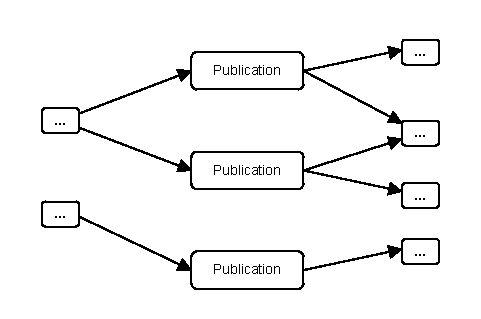
\includegraphics[width=0.75\textwidth]{figures/figures-RKG_structure.drawio.pdf}
    \caption[Example Structure of an RKG]{Example structure of an \gls{rkg}. Here, the information of interest is gathered as a subgraph around nodes of type \emph{Publication}. HubLink uses these subgraphs by encoding them as Hubs to perform targeted inference.}
    \label{fig:rkg_structure}
\end{figure}

When retrieving data from a graph, it is important to ensure that the relationships between information are retained correctly to avoid losing valuable data. This can be challenging, as it is not always clear how much of the surrounding information is actually needed \cite{peng_graph_2024,hu_grag_2024}. Our solution to this challenge is to decompose the graph into distinct \texttt{Hub} structures. This design choice is informed by the way information is organized within an \gls{rkg}. As observed by \textcite{verma_scholarly_2023}, an \gls{rkg} stores scientific data through research entities. Due to the inherent structure of graphs, related data tends to cluster around these entities. In this setup, the research entities act as roots, aggregating scientific information through their neighboring nodes. 

\autoref{fig:rkg_structure} illustrates this concept. It shows entities of the \emph{Publication} type that inherently store scientific information about the publication around them. In this case, each publication entity serves as a root, with its associated data stored in the surrounding nodes. Given that questions in scholarly \gls{kgqa} typically target information related to research entities, this natural clustering is exploited in the retrieval strategy of HubLink. We refer to this cohesive unit of information as a \texttt{Hub}, where each hub is based on a root node and encompasses all semantically related information accessible through paths originating from it.

Encoding these hubs in a vector space requires careful consideration of two key aspects: a) the significance of a node relative to the root node of the hub, and b) the preservation of relationships among the nodes within the hub. To meet both criteria, we consider all directed paths within the hub that start at the root and lead to end nodes. These paths are referred to as \texttt{HubPaths}. At the core, each \texttt{HubPath} represents a directed path within a hub that starts at the root entity of the hub, follows the direction of the graph, and either a) continues to the end of the graph, b) reaches a predetermined maximum length, or c) encounters a new root node of another hub. The idea of a \texttt{HubPath} is that the information on the path shares a common semantic meaning and should be encoded together in the vector space. Therefore, each \texttt{HubPath} is converted to vectors during indexing and stored in a vector database.


\subsection{Applying a Diversity Ranker on the Triple Level}

During development, we encountered an issue caused by retrieving triple-level vectors from the index. Since it is common that multiple triples $(s,p,o)$ share the same subject $s$, this leads to a situation where many irrelevant triples receive a high similarity score simply because they share the same subject. This creates a problem during retrieval in which only a fixed number of \texttt{HubPaths} are selected per candidate hub.
% The retrieved paths often add no value to answering the question because they all have the same subject entity, which by itself has a high relevance to the query, but the remaining information in the triple has not.

To illustrate this, consider the following question: \enquote{Which authors does the paper with the title 'A Complexity Metric for Microservices Architecture Migration' have?}. When this question is processed, it is decomposed into several components, one of which includes the paper title. Then, a similarity search is performed using these components. If the graph contains many triples where the title is the subject, these triples may dominate the top results due to the strong subject match, regardless of whether their predicates and objects are actually useful for answering the question. This effect can crowd out more relevant triples, such as those identifying the authors, from the top-k ranked \texttt{HubPaths} for a hub.

To mitigate this issue, we introduce a \emph{Diversity Ranker}. This component penalizes triples whose subject has already been encountered, thereby encouraging a more diverse set of \texttt{HubPaths} in the results. This increases the chances of retrieving paths that contribute novel and useful information. 

\subsection{Using Weighted Averaging for Scoring of Hubs}

In earlier stages of development, we calculated the score of a hub by taking the average of all associated \texttt{HubPath} objects. However, this approach revealed an issue that led us to adopt a weighted mean instead. Originally, the unweighted hub score was calculated as:

\[
\text{Score}(Hub) = \frac{1}{n} \sum_{i=1}^{n} \text{Score}(h_i), \quad h_i \in \mathcal{H}
\]

Here, \( \mathcal{H} \) denotes the set of all \texttt{HubPath} objects for a given hub, \( h_1, \dots, h_n \) are the individual paths, and \( n \) is the number of these paths. The main drawback of this method is that all paths are treated equally, regardless of their individual relevance. As a result, a hub with many average-quality paths could end up with a higher total score than a hub that has fewer but highly relevant paths. This leads to a situation where important paths with high scores are overshadowed by a large number of less relevant ones, even though they might be critical for the overall quality of the hub. To address this issue, we now use a weighted mean, where paths with higher scores contribute more significantly to the overall score of the hub. Formally, let \( \vec{s} = [s_1, s_2, \dots, s_n] \) be the list of scores of all paths for a given hub. The weights for this new calculation are computed as follows:

\[
w_i = \exp(\alpha \cdot s_i)
\]

The final weighted score of the hub is then given by:

\[
\text{Score}(Hub) = \frac{\sum_{i=1}^{n} w_i \cdot s_i}{\sum_{i=1}^{n} w_i}
\]

The parameter \( \alpha \) controls the extent to which high path scores are emphasized. Furthermore, this parameter can be fine-tuned to adapt to any given context. 


\subsection{Enriching Hubs by Linking to External Data}

Although representing information as a graph introduces structure and emphasizes semantic relationships, it also comes with a trade-off: a loss of textual detail. This occurs because textual content must be adapted to the \gls{rdf} format, which fragments information into triples, each capturing only a small portion of the original narrative. The goal of the linking process in HubLink is to complement the structured graph data with additional, richer context from external sources. This should enhance answer generation by providing more complete and informative responses.


To illustrate, consider a literature search scenario in which individual papers serve as the hub objects. Each hub is associated with a unique identifier, typically the DOI of the paper. This identifier enables the retrieval of additional information beyond what is captured in the graph. For example, we may connect to an external vector store that holds embeddings of the full-text from papers. Once relevant hub candidates are identified, the linking process uses their DOIs to perform targeted nearest-neighbor searches on these text embeddings. The returned text segments are then used to enrich the knowledge of the corresponding hubs. By combining structured graph data with context-rich textual extracts, this process can lead to more comprehensive and nuanced answers. In addition, it supports transparency in the retrieval process, as the enriched responses can be directly traced back to their source documents.



\subsection{Providing Two Different Retrieval Strategies} 

During the development of HubLink, we decided to implement two different retrieval strategies. This decision was driven by a trade-off that emerged during development. By introducing both strategies, we allow users to choose the strategy that best suits their specific use case. In the following, we take a closer look at this trade-off.

The first approach, \emph{direct retrieval}, enables fast retrieval using the vector index to quickly identify semantically similar content. Although this method is efficient and scalable, it becomes less effective in retrieving localized information as the size of the index grows. When multiple contexts from different sources share semantic similarity with the query, they may all be retrieved, regardless of whether they are relevant to the specific intent of the question. This can be problematic for questions that are meant to target particular segments of the knowledge graph.

To mitigate this limitation, traditional search systems often use metadata filters (e.g., research field, publisher, publication year) to narrow the scope of search results. HubLink incorporates a similar principle in its second strategy, \emph{graph traversal retrieval}. In this approach, a specific entry point in the graph, referred to as a topic entity, is used to constrain the search to a relevant subregion of the graph. Without such a focus, the system would need to search the entire graph, increasing the risk of retrieving irrelevant information from unrelated areas. Consequently, the topic entity effectively acts as a filter, making this strategy particularly valuable in large-scale graphs containing millions of nodes.

However, using the \emph{graph traversal retrieval} strategy comes with the drawback that a topic entity must be known or inferred. In some cases, such an entity may already be known. For example, if it is already known that a question refers to publications of a specific research field, the entity of that research field could be provided as input. Alternatively, the topic entity may be extracted automatically from the question, for example, through \emph{named entity recognition} as demonstrated in \cite{wang_reasoning_2024}. Here, the terms provided in the question are mapped to entities in the graph using an \gls{llm} process. 

Furthermore, another drawback of the \emph{graph traversal retrieval} strategy is that traversing the graph is time-consuming and adds computational expense. This is because the hubs must be found by traversing the graph, which is a complex process that can take a considerable amount of time depending on the size of the graph and the number of hubs. The time requirement increases even further if the initial hubs do not provide an answer, and deeper levels must be traversed. Thus, the trade-off between the two retrieval strategies becomes increasingly relevant as the graph grows in size: it is a balance between the accuracy of the results and the computational cost and runtime. Consequently, we decided not to enforce a one-size-fits-all solution. Instead, users should choose the strategy that best fits their specific use case and requirements.

\subsection{Prompt Engineering}

The HubLink algorithm includes a total of four prompts, which are presented in Appendix~\ref{sec:appendix:hublink_prompts}. During development, we observed that the performance of HubLink strongly depends on whether the prompts actually achieve the goal for which they are used. This is particularly true when generating partial answers. If the task description is too vague, too much irrelevant information will be included, and if it is too restrictive, too little information will be included. In the following, we briefly introduce our rationale behind each of the prompts in HubLink.

\paragraph{Partial Answer Generation Prompt} This prompt is responsible for creating a partial answer for each hub. It is important here that even if the hub does not fully answer the posed question, all partial information provided by the hub for the given answer is formulated into a partial answer. We therefore created a prompt that prioritizes the integration of partial information even if it is not yet apparent whether the information is actually useful for the final answer later on. To support the \gls{llm} in understanding the task, we created a few-shot prompt that demonstrates how partial answers should be created from the hub information.

\paragraph{Final Answer Generation Prompt} This prompt receives all created partial answers and generates a final answer by aggregating all partial answers. In addition, the \gls{llm} has the task of marking every fact in the answer with a source in the form of $[i]$. With this, we want to ensure that transparency about the information source is guaranteed during answer creation, which is particularly important in the scientific field. At the end of the generated answer, a list with the DOI and the title of the publication is appended.

\paragraph{Question Component Extraction Prompt} This prompt is used to extract the components of the question from the given query. Here, we created a few-shot prompt to show the \gls{llm} the desired granularity for extraction.

\paragraph{Triple Filtering Prompt} This is the last prompt in the execution. Here, based on the posed question, the answer, and the triples, a decision is made as to which triples are most relevant to the answer to filter out those triples that are not needed.

It should also be mentioned here that, depending on the application case, it may be reasonable to make adjustments to the current prompts. For example, during partial answer generation, the focus could be on identifying contradictions between sources instead of a simple synthesis of information.

\section{Generalizability and Scalability}
\label{sec:hublink_generality_and_chances}

The fundamental design of HubLink offers potential regarding its range of application and performance capabilities. This section discusses these aspects. First, we explain why we consider HubLink to be schema-agnostic. Then, we examine the adaptability of the approach to other domains. Last, we explore the scalability of the approach by discussing how the modularity of the approach facilitates efficient processing even on \glspl{kg} comprising millions of entities and relations.

\subsection{Why HubLink is Schema-Agnostic}
% This means that it does not make assumptions about the particular vocabulary or ontology used in the underlying \gls{kg} and consequently, does not rely on a fixed set of entity types or relation predicates. 
% Training based but schema agnostic: LLMs
% Training based and not schema agnostic: Semantic Parsing
% not schema agnostic: Semantic parsing with examples

We define \emph{schema-agnostic} as a characteristic of a system that does not rely on a fixed schema (i.e., a predefined set of classes, predicates, or relations). Instead, such a system operates on arbitrary or previously unseen graph structures without requiring adaptation of its core functionality.

HubLink is designed to be schema-agnostic because all core processing steps, including graph traversal, extraction, embedding, and retrieval, work on generic triples. Consequently, HubLink does not depend on any particular classes, property names, or specific ontology structures. This design makes the approach directly applicable to graphs with diverse or evolving schemas without necessitating changes to the underlying algorithms.

Nevertheless, the implementation of the \textsc{isHubRoot} classification function introduces a point where schema awareness can be incorporated, particularly if classification relies on entity types. The degree of sensitivity to schema evolution in such instances depends on the specific implementation chosen. For example, in the experimental setting conducted for this thesis, the \emph{Paper} type from the \gls{orkg} served as a criterion for \texttt{HubRoot} classification. We argue that this specific choice does not render the overall approach inherently schema-reliant. This argument is supported by two main points: first, the designated type is fundamental to the graph structure in that context and is not anticipated to undergo frequent changes. Second, the construction and retrieval of paths within hubs remain entirely independent of schema-defined types. Furthermore, as defined in Section~\ref{sec:hublink_hubroot_definition}, the HubLink approach supports alternative methods for classifying \texttt{HubRoots} that do not use any direct schema information from the graph, thus offering a mechanism to maintain schema independence even in the hub classification stage.


% Although schema information can optionally be used as a criterion for the \texttt{isHubRoot} classification function, this is not a requirement. Even if specific types are used to define which nodes serve as hub roots, the construction and retrieval of paths within those hubs remain entirely schema-agnostic. This ensures that HubLink can operate flexibly on heterogeneous graphs.

\subsection{Applicability to Other Domains}

Although the current implementation of HubLink has focused on \glspl{rkg}, which store scientific data, the approach is not limited to this domain. We believe that HubLink is broadly applicable to any field where the knowledge base is organized around well-defined entities. This includes domains such as internal company documents, Wikipedia articles, medical case records, or biological entities such as genes or proteins.

The key strength of HubLink lies in its ability to extract, aggregate, and retrieve information centered around specific objects. If these objects of interest are identifiable within the given data context, they can be used as hubs, making HubLink a flexible and adaptable solution across diverse domains. 

\subsection{Scalability to Large Graphs}

In addition to cross-domain applicability, scalability is a critical factor for the practical use of HubLink. Although large-scale evaluations fall outside the scope of this thesis, we argue that HubLink is well suited for deployment on \glspl{kg} containing millions of triples. This is because a unique advantage of HubLink lies in its modular, hub-based design. For queries that span multiple subgraphs or require aggregating information from distributed sources, the HubLink approach allows the graph to be decomposed into hubs. Each hub can then be individually evaluated to determine whether it contributes to answering the query. This allows the system to scale horizontally by distributing the evaluation across multiple hubs or even machines. This modular approach has the potential to handle complex queries efficiently by dividing the problem into smaller subproblems. We argue that HubLink opens up new possibilities for scalable and intelligent retrieval across large and complex \glspl{kg}. 

To realize the indexing of large-scale graphs, we propose two complementary strategies:

\paragraph{Indexing the entire Graph:} 
One possible strategy is to index the entire graph using the embedding-based method of HubLink. Since the vector similarity search does not scale linearly with the size of the graph, response times remain relatively stable even as the graph grows. However, this property applies exclusively to the \emph{direct retrieval} strategy because, in contrast, the \emph{graph traversal} strategy requires evaluating all hubs that can be reached from the topic entity. However, this makes the traversal strategy particularly effective for queries targeting a specific region of the graph, as the topic entity naturally constrains the retrieval scope, leading to more focused searches.

\paragraph{Partitioning the Graph:} 
An alternative approach that would also allow for control of the retrieval section involves partitioning the graph into multiple indices. This method proves advantageous when the relevant semantic domain of a query is known in advance. The underlying assumption is that large-scale \glspl{kg} can be divided into semantically coherent subgraphs. Once such segmentation is performed, indexing can be limited to the subgraphs that are relevant to the queries. Consequently, it becomes necessary to select the appropriate index before processing a question. This selection can be carried out manually or automatically, for example, through an \gls{llm}-based classification mechanism.

% To improve efficiency, the update process can be optimized by leveraging the timestamps of the modified triples, as only those paths affected by actual changes need to be removed and rebuilt, thereby avoiding the unnecessary reconstruction of unaffected components.

\section{Updating the Index}
\label{sec:updating_the_index}

The HubLink retriever can only respond to questions based on the information stored in the associated index. For this reason, it is essential to update the index whenever changes are made to the graph to ensure that the data remains consistent and up-to-date. The following section explains how this update process can be implemented.

As illustrated in the pseudocode of the function \textsc{hubIndexNeedsToBeUpdated}, changes in individual hubs can be detected by comparing the hash values of the current \texttt{HubPath} objects with those stored in the index. A mismatch indicates a modification and thereby signals the need for an update. Alternatively, if each triple in the graph is annotated with a timestamp indicating its last modification, this metadata can also serve as a criterion for determining whether an update is required. When a hub is identified as outdated, it can then be refreshed by invoking the \textsc{buildHubs} method. This procedure removes outdated entries from the index and rebuilds the corresponding \texttt{HubPaths}. 

The pseudocode in Section~\ref{sec:hublink_indexing} demonstrates how the index update can be implemented. This indexing function is designed to serve both initialization and maintenance purposes. During an update run, the algorithm iterates through each hub, verifying whether the paths stored in the graph remain consistent with those in the index. If discrepancies are detected, the affected components are updated accordingly. This procedure, which we refer to as the \emph{Fixed Update} strategy, entails a comprehensive review of the index performed at specified intervals. Although computationally intensive, this approach guarantees that the entire index is synchronized upon completion.

An alternative strategy is the \emph{Dynamic Update}, wherein updates are executed in real time in response to changes in the graph. When a modification occurs, the affected hubs are immediately updated using the \textsc{buildHubs} method. This method requires the integration of a monitoring routine that is automatically triggered upon any update to the graph. Such a routine can either invoke \textsc{buildHubs} directly or interact with the vector index to selectively adjust the relevant data entries.

In summary, we propose the following two strategies to maintain index consistency:

\begin{itemize} 
    \item \textbf{Fixed Update:} Involves a complete and periodic examination of the index to identify and refresh outdated hubs. This process is performed at predefined intervals and ensures full synchronization.
    \item \textbf{Dynamic Update:} Executes updates immediately following any modification to the graph. A monitoring routine initiates the update process, targeting only the affected components.
\end{itemize}



\section{Limitations}
\label{sec:hublink_limitations}

The primary limitation of HubLink is the requirement of an index. This index is crucial for inference because only the information stored in the index is seen by the retriever. Consequently, if a question asks for information that is not indexed as part of a hub, it is not considered. This requires careful management of the index, for which we outline several possibilities in Section~\ref{sec:updating_the_index}. Nevertheless, we argue that using an index instead of training is a considerable benefit, as building the index itself does not require any additional data but the graph itself.

Beyond the limitation of the index, several other considerations affect the HubLink approach. The definition of optimal criteria to classify \texttt{HubRoot} entities from which the hubs are built is not straightforward and depends on the underlying graph. If these criteria are not well defined, relevant information may not be encapsulated within hubs, rendering it unreachable until the criteria and index are updated.

Furthermore, the indexing process itself, particularly for large or frequently updated graphs, can be computationally intensive and time-consuming. In addition, the decomposition of paths into multiple vector representations during indexing contributes to increased storage requirements of the index. These factors introduce maintenance overhead, as changes in the graph necessitate updates to the HubLink index.

Moreover, the answer generation capabilities of HubLink are significantly dependent on the \gls{llm} utilized. Whether the \gls{llm} is able to pre-filter extraneous information during the generation of partial answers and subsequently synthesize these into a coherent final answer relies upon the performance of the \gls{llm} and also whether the prompts are clear and specific enough for the \gls{llm} to understand. This may require the adaptation of prompts for different \glspl{llm}, tasks, or domains to achieve optimal results.

Operational aspects also introduce limitations. For instance, the graph traversal retrieval strategy requires a topic entity as an input, which implies either user provision or an auxiliary mechanism for entity linking from the query. Additionally, HubLink is an embedding-based system at its core and, as such, inherits certain limitations common to these types of systems. For example, as described by \textcite{wang_reasoning_2024}, the processing and interpretation of numerical constraints, such as dates, value ranges, or specific metric comparisons, presents challenges for such systems.

% If the information that is asked for is not indexed as part of a hub, it can't be found by the retriever. This is a limitation of the retrieval process, as the retriever can only find information that is part of a hub.

% The definition of the optimal criteria to classify HubRoots is not straightforward, as it depends on the underlying graph ontology. If the criteria is not well defined, relevant information might not be encapsulated within hubs, making it undiscoverable during retrieval.

% If new types of entities or relationships are added into the RKG, and they do not fit the existing HubRoot classification criteria or are not part of any current hub, they will not be indexed and thus the system will not be able to retrieve information about it until the HubRoot criteria is updated.

% Especially for large graphs, the indexing process can be computationally expansive and time-consuming. Future graph updates necessitate an update to the index. If these updates are frequent this can lead to a significant overhead. Furthermore, as a graph provider, in addition to the graph itself, the index of HubLink has to be managed as well which adds further maintenance costs.

% The decomposition of paths during the indexing process increases the size of the index requiring more overall storage.

% The answer generation heavily depends on prompt engineering. It is important that during the generation of partial answers, the LLM pre filters unnecessary information and moves forward those information that could potentially be relevant for the final answer. Consequently, the generation of the final answer needs to be able to synthesize all relevnt information from the partial answers, which depends on the prompt engineering instructions. COnsequently, it might be necessary to adapt the prompts for specific tasks as a general prompt might not be sufficient for all scenarios.

% The graph traversal strategy requires a topic entity as input. This requires either the user to provide such an entity or a automatic procedure that maps the question to an appropriate entity in the graph. An example for such an approach can be found in the work of \textcite{wang_reasoning_2024}.

% For complex queries or in dense graph regions, the number of candidate hubs and paths can become very large, impacting the performance of ranking, pruning, and subsequent LLM processing steps.

% The processing of numerical constraints, such as dates, ranges of values or specific metric comparisons, presents a potential challenge for embedding-based retrieval approaches like HubLink, as highlighted in previous research \cite{jin_floating-point_2024}.






\chapter{Taxonomy Construction Methodology}
\label{ch:taxonomy_construction_approach}

This section presents Contribution \hyperref[enum:c2]{\textbf{C2.1}}, a taxonomy construction methodology that aims to systematically compile knowledge from the literature to create an initial taxonomy, which is then improved and validated. The approach draws inspiration from the revised construction method by \textcite{usman_taxonomies_2017} by adapting the proposed \emph{planning}, \emph{identification and extraction}, \emph{design and construction}, and \emph{validation} phases.

The chapter is organized as follows. In Section~\ref{sec:taxonomy_evaluation_plan} we first describe an evaluation plan that outlines how a taxonomy can be evaluated according to a \gls{gqm} model. Then, in Section~\ref{sec:taxonomy_development_process} our proposed taxonomy construction process is presented.


\section{Evaluation Plan}
\label{sec:taxonomy_evaluation_plan}

\begin{table}[t]
\centering
\resizebox{\textwidth}{!}{%
\begin{tabularx}{\textwidth}{p{0.3\textwidth} X X}
\toprule
\textbf{Goal} & \textbf{Question} & \textbf{Metric} \\
\midrule
\multirow{3}{=}{\textbf{G1} Validate the suitability of the taxonomy by checking that it allows objects under study to be classified appropriately, with the correct scope and level of detail.} 
& \textbf{Q1.1} Has the taxonomy reached an appropriate level of generality and granularity? 
& \textbf{M1.1.1} Laconicity \newline \textbf{M2.1.2} Lucidity \\
\cmidrule(lr){2-3}
& \textbf{Q1.2} Is the taxonomy appropriate, comprising only necessary classes? 
& \textbf{M1.2.1} Completeness \newline \textbf{M2.2.2} Soundness \\
\cmidrule(lr){2-3}
& \textbf{Q1.3} Is the taxonomy orthogonal without overlapping classes? 
& \textbf{M1.3.1} Orthogonality \newline matrix \\
\cmidrule(lr){2-3}
\multirow{3}{=}{\textbf{G2} Assess the quality and relevance of the taxonomy to existing ones to validate its purpose.} 
& \textbf{Q2.1} Is the taxonomy relevant, comprising only necessary classes and categories? 
& \textbf{M2.1.1} Fraction of relevant classes and categories \\
\cmidrule(lr){2-3}
& \textbf{Q2.2} Is the taxonomy novel, having the right extent of new categories?
& \textbf{M2.2.1} Innovation \newline \textbf{M2.2.2} adaption \\
\cmidrule(lr){2-3}
& \textbf{Q2.3} Is the taxonomy significant which enables a more precise description?
& \textbf{M2.3.1} Classification Delta \\
\bottomrule
\end{tabularx}%
}
\caption[GQM Plan for Taxonomy Validation]{Overview of the \gls{gqm} plan for the validation of the taxonomy.}
\label{tab:gqm_taxonomy_validation}
\end{table}

This section includes an evaluation plan which is applied in the validation and application phases of our proposed taxonomy construction process. The plan is implemented following the \gls{gqm} method \cite{basili_methodology_1984,basili_software_1992} and is illustrated in \autoref{tab:gqm_taxonomy_validation}. The plan consists of two goals with a total of six questions and nine metrics. The metrics are based on the taxonomy evaluation approach proposed by \autocite{kaplan_introducing_2022} and are described in Section~\ref{sec:fund_evaluating_taxonomy}.

The first goal, \textbf{G1}, concentrates on validating the \emph{suitability} of the taxonomy. It seeks to confirm that the taxonomy allows for the appropriate classification of the objects under study, maintaining the correct scope and level of granularity. Three questions address this goal. \textbf{Q1.1} evaluates whether the taxonomy achieves an appropriate level of generality and granularity. An insufficient number of classes may reduce informational utility, whereas an excessive number can introduce unnecessary complexity, hindering effective application. \textbf{Q1.2} assesses appropriateness, focusing on whether the taxonomy encompasses all necessary categories while excluding unnecessary ones. This involves balancing the inclusion of classifications required for comprehensive characterization against the avoidance of rarely utilized categories. \textbf{Q1.3} examines orthogonality, evaluating the degree of overlap among categories. Low orthogonality indicates redundancy due to overlapping categories. Minimizing such overlap enhances the precision of classification.

The second goal, \textbf{G2}, relates to the validation of the purpose of the taxonomy by assessing its quality and relevance relative to existing taxonomies. This goal encompasses three questions. \textbf{Q2.1} assesses the relevance of the classes and categories concerning the stated objectives of the taxonomy. This involves demonstrating the necessity of each element for fulfilling the intended function of the taxonomy. Question \textbf{Q2.2} investigates the novelty of the taxonomy, specifically the extent to which it introduces new classes or adapts existing ones compared to established taxonomies. Finally, \textbf{Q2.3} evaluates the  significance by determining whether the taxonomy facilitates a more precise description or classification within its domain than preceding taxonomies permit.

% \subsection{Validating the Suitability}

% 

% \textbf{Q2.1} concerns verifying that the taxonomy is neither too broad nor too specific. It is about finding an appropriate level of granularity. A low number of classes diminishes information utility, whereas an excessive number introduces noise, complicating taxonomy application. We quantify the generality and granularity using the \emph{laconicity} and \emph{lucidity} metrics \cite{kaplan_introducing_2022}. The second question \textbf{Q2.2} addresses the appropriateness, focusing on whether the taxonomy includes sufficient categories without any that are unnecessary. It is about maintaining the trade-off between adding classifications that are required to sufficiently classify the characteristics of a \gls{kgqa} system, without introducing categories that are never used. To quantify the appropriateness, the \emph{completeness} and \emph{soundness} metrics are used \cite{kaplan_introducing_2022}. The third question \textbf{Q2.3} addresses the orthogonality, which is about the evaluation of whether the taxonomy has overlapping categories. If the orthogonality is low, the taxonomy has overlapping categories which can be removed to increase preciseness. If issues are found during this validation step, the development process returns to the taxonomy refinement step to correct the shortcomings. The result is a new increment of the taxonomy which has to be validated once again. 

% \subsection{Validating the Purpose}

\section{Development Process}
\label{sec:taxonomy_development_process}

\begin{figure}[t]
    \centering
    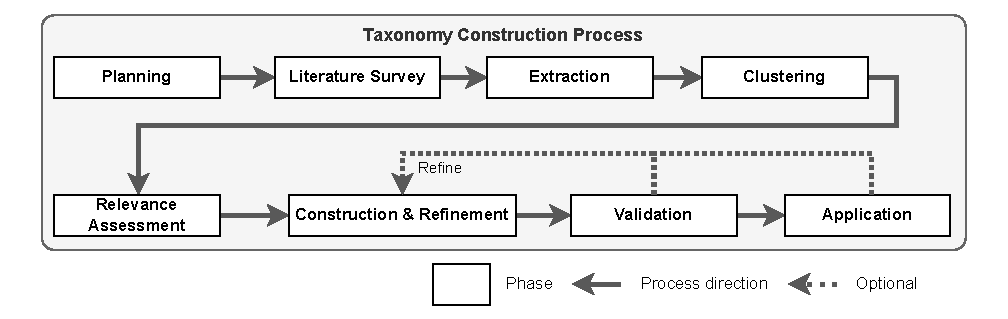
\includegraphics[width=0.99\linewidth]{figures/question_catalog/taxonomy-construction_process_general.drawio.pdf}
    \caption[Taxonomy Construction Process]{The taxonomy construction process involving eight consecutive phases to synthesize knowledge from the literature into a taxonomy that is then incrementally refined and validated.}
    \label{fig:taxonomy_development_process}
\end{figure}

The overall development process is illustrated in \autoref{fig:taxonomy_development_process}. It consists of eight consecutive phases. The process begins with the \textsc{Planning} phase, where the intended use of the taxonomy is defined. In the following \textsc{Literature Survey} phase, a literature review is conducted to collect potential candidates that contain relevant terms, which we refer to as classes. These candidates are then manually extracted in the \textsc{Extraction} phase to identify the relevant classes from the text. In the \textsc{Clustering} phase, the extracted classes are merged in a deduplication process and subsequently grouped into semantic categories. These categories are then evaluated for their relevance in the \textsc{Relevance Assessment} phase. The remaining categories are used to initialize the first taxonomy increment during the \textsc{Construction and Refinement} phase. This increment is then evaluated in the \textsc{Validation} phase to determine whether revisions are necessary. If so, the process returns to the previous phase. Otherwise, it proceeds to the \textsc{Application} phase, where the practical use of the taxonomy is demonstrated in a specific application scenario. In the following sections, we take a closer look at each phase of the process.


\subsection{Planning}
\label{sec:tax_dev_planning}

The first phase of the process is \textsc{Planning}. In this phase, the objective and intended use of the taxonomy is defined. Additionally, characteristics of the taxonomy that should be considered during its development are specified.

According to \textcite{usman_taxonomies_2017}, six activities should be carried out when planning a taxonomy. However, it is important to note that the authors focused specifically on the software engineering domain. For our process, we aim to maintain general applicability. Therefore, we have adapted these activities and formulated the following steps for the \textsc{Planning} phase:


\begin{enumerate}[label=\textbf{S\arabic*:}, leftmargin=2.5em]
    \item \label{enum:step1} Define one or more declarative sentences that clearly define the objective and scope of the taxonomy.
    \item \label{enum:step2} Define the domain for which the taxonomy is to be applied.
    \item \label{enum:step3} Define the structure type of the taxonomy.
    \item \label{enum:step4} Define the procedure type of the taxonomy.
    \item \label{enum:step5} Define the topics and domains of the literature from which the collection of classes takes place.
\end{enumerate}

In the first step, \textbf{S1}, the goal of the taxonomy should be clearly defined so that users understand the use cases it is meant to support. To achieve this, one or more declarative sentences should be formulated that narrow the scope and clearly express the intended purpose. 

Step \textbf{S2} involves defining the domain of the taxonomy. This should help users assess whether the taxonomy is intended for a specific domain and allow them to better understand its scope.

In \textbf{S3}, the structure of the taxonomy is specified. According to \textcite{usman_taxonomies_2017}, there are four different types of structures, which we will explain briefly. A taxonomy with a \emph{hierarchy} structure has a single parent class that contains multiple subclasses. In contrast, a \emph{tree} structure does not imply inheritance relationships between classes. Instead, it features a parent class with subclasses that can represent relationships such as part-whole, cause-effect, and process-product. A \emph{paradigm} taxonomy represents a two-dimensional matrix classification, where each cell represents a combination of possible classes. Finally, a \emph{faceted} taxonomy captures multiple independent perspectives or \enquote{facets}, each with its own set of classes.

In step \textbf{S4}, the procedural type of the taxonomy has to be defined. This procedure describes how instances are systematically assigned to the classes or categories of the taxonomy. The procedure depends on the measurement method used for the classification and is divided into two types, according to \textcite{usman_taxonomies_2017}. \emph{Qualitative} procedures use nominal scales, which means that the classification is based on descriptive attributes. \emph{Quantitative} procedures, on the other hand, use numerical scales for classification.

The final step in the planning phase is \textbf{S5}, which involves categorizing the literature from which the classes will be extracted according to their topics and domains. This helps users understand the data foundation from which the taxonomy has been derived.

\subsection{Literature Survey}
\label{sec:tax_con_literature_survey}

The second phase of the development process is named \textsc{Literature Survey}. The goal is to identify candidates from the literature that potentially contain relevant classes for the taxonomy. The survey is conducted iteratively, with transparency and repeatability serving as top priorities. Furthermore, this iterative approach allows the process to be paused early if needed and resumed at a later time. 

Two lists are defined to conduct the literature survey: \emph{Intermediate List} and \emph{Final List}. The intermediate list is defined for each iteration and is denoted as $\mathcal{L}_i$, where $i \in \mathbb{N}_{>0}$ indicates the current iteration. This list contains all the literature resources that have been processed during that specific iteration. This processing is done using the \hyperref[enum:processing_paper_task]{\textbf{Processing Paper Task}} described below. During this task, new candidates may be extracted from a resource $\mathcal{P}$, which then forms the list for the next iteration, $\mathcal{L}_{i+1}$, such that:

\[
\mathcal{L}_{i+1} = \bigcup_{\mathcal{P} \in \mathcal{L}_i} \left( \text{Ref}(\mathcal{P}) \cup \text{CitedBy}_n(\mathcal{P}) \right)
\]

Here, $\text{Ref}(\mathcal{P})$ refers to the set of relevant references from the bibliography of $\mathcal{P}$, while $\text{CitedBy}_n(\mathcal{P})$ represents the first $n$ publications assessed as relevant from a \emph{Cited by} search. 

In addition, the literature survey process has a second list named \emph{final list} which is denoted as $\mathcal{F}$. This list contains all literature resources that have been assessed as relevant in any of the conducted iterations of the process.

The following section illustrates the literature survey process, which is based on the guidelines for conducting a systematic literature review by \textcite{wohlin_guidelines_2014}:


\paragraph{Literature Survey Process}
\begin{enumerate}
    \item \textbf{Prepare Seeds:} Collect seed papers and add them to $\mathcal{L}_1$.
    \item \textbf{First Iteration:} Process each paper in $\mathcal{L}_1$ by applying the \emph{Processing Paper Task} described below.
    \item \textbf{Additional Search:} Conduct a search e.g. on Google Scholar to find additional papers that are not covered by the seed papers. Add these papers to $\mathcal{L}_2$.
    \item \textbf{More Iterations:} Process each paper in the intermediate list of the current iteration $i \in \mathbb{N}_{>0}$ by applying the \emph{Processing Paper Task} described below. Continue processing until satisfied or there are no more paper candidates in $\mathcal{L}_i$.
\end{enumerate}

\paragraph{Processing Paper Task}
\label{enum:processing_paper_task}
\begin{enumerate}
    \item Collect paper $\mathcal{P}$ from $\mathcal{L}_i$ that has not yet been processed.
    \item Determine whether $\mathcal{P}$ is relevant on the basis of the title and abstract. This is done by applying the defined \emph{inclusion} and \emph{exclusion} criteria. If not relevant, $\mathcal{P}$ is skipped.
    \item The text of $\mathcal{P}$ is skimmed to identify relevant text sections. If no relevant text sections are found, $\mathcal{P}$ is skipped.
    \item If $\mathcal{P}$ is found to be relevant, it is added to the list $\mathcal{F}$.
    \item The reference list of $\mathcal{P}$ is processed to identify possible relevant publications based on their title. Add these candidates to the $\mathcal{L}_{i+1}$.
    \item Using a search engine like Google Scholar, the \emph{cited by} feature is used on $\mathcal{P}$ to collect a list of publications $\hat{\mathcal{C}}$ referencing $\mathcal{P}$. The list is obtained by sorting by relevance and collecting the first $n$ publications. For each $\hat{\mathcal{c}} \in\hat{\mathcal{C}}$, their titles and abstracts are analyzed to consider whether the defined \emph{inclusion} and \emph{exclusion} criteria are met. If so, the paper $\hat{\mathcal{c}}$ is added to $\mathcal{L}_{i+1}$.
\end{enumerate}

To help categorize publications as relevant, inclusion and exclusion criteria should be defined. The exact criteria used depend on the respective objective and domain of the taxonomy.

\subsection{Extraction}

The result of the literature search is the set $\mathcal{F}$, which includes all publications that were classified as relevant. In the \textsc{Extraction} phase, each publication $f \in \mathcal{F}$ is processed by identifying classes for the taxonomy based on the content of the publication. For each relevant publication $f$, a subset $\mathcal{C}_{f}$ is defined, containing all classes extracted from $f$. Each class consists of a name and a description, both taken directly from the respective publication.

The complete set of all extracted classes is defined as the union of all $\mathcal{C}_{f}$ for every $f \in \mathcal{F}$:

\[
\mathcal{C} = \bigcup_{f \in \mathcal{F}} \mathcal{C}_{f}
\]


\subsection{Clustering}
\label{sec:tax_proc_clustering}

The next phase is called \textsc{Clustering} and consists of two main steps. First, the classes $\mathcal{C}$ extracted from the literature are grouped to merge semantically redundant entries. Then, these consolidated classes are organized into categories.

\paragraph{Deduplication}
In the first step, the extracted classes $\mathcal{C}$ are clustered based on their semantic similarity. Classes that are considered equivalent or very similar in meaning, based on their names or descriptions, are grouped together. The level of abstraction at which this merging occurs depends on the specific use case.

Each resulting cluster contains classes that are either semantically equivalent or closely related. The set of these clusters is denoted by $\hat{\mathcal{C}} = {\hat{c}_1, \hat{c}_2, \dots, \hat{c}_n}$, where each cluster $\hat{c}_i$ is a subset of the original class set $\mathcal{C}$, and all clusters are mutually disjoint:

\[
\forall i \ne j: \hat{c}_i \cap \hat{c}_j = \emptyset
\quad \text{and} \quad \bigcup_{i=1}^{n} \hat{c}_i = \mathcal{C}
\]

For each cluster $\hat{c}_i$, a representative class is defined, which provides the cluster with a name and description. This can be done either by selecting an existing class within the cluster or by manually synthesizing a new one based on the contained classes.

\paragraph{Categorization}
In the second step, the class clusters $\hat{\mathcal{C}}$ are grouped into semantically coherent categories, denoted as $\mathcal{K}$. Depending on the context, it may be assumed that these categories are disjoint. Each category $k \in \mathcal{K}$ is assigned a name $n_k$ and a description $d_k$. Naming is based on the interpretation of the deduplicated classes contained in $\hat{C}_k$, with the aim of capturing the overarching semantic context of the included concepts. The description $d_k$ provides clarification and contextual background for the category. A category can thus be represented as a tuple:

\[
k = (\hat{C}_k, n_k, d_k)
\]

Here, $\hat{C}_k \subseteq \hat{\mathcal{C}}$ is the associated group of deduplicated classes, $n_k$ is the name of the category, and $d_k$ is the corresponding description. The complete set of categories is then:

\[
\mathcal{K} = \left\{ (\hat{C}_k, n_k, d_k) \;\middle|\; \hat{C}_k \subseteq \hat{\mathcal{C}} \right\}
\]

\subsection{Relevance Assessment}

During the \textsc{Relevance Assessment} phase, the goal is to evaluate the set of categories $\mathcal{K}$ and their corresponding deduplicated classes $\hat{C}_k$ in terms of their relevance to the target taxonomy. This step reduces the overall set $\mathcal{K}$ to only the categories and classes that are truly significant.

To assess relevance, an evaluation function is defined based on a specified set of qualitative criteria. Each category and class are manually evaluated through content analysis and reasoned judgment. The evaluation function is formalized as follows:

\[
\text{rel}: \hat{\mathcal{C}} \cup \mathcal{K} \rightarrow \{0, 1\}
\]

Where: 
\begin{enumerate} 
    \item $\text{rel}(x) = 1$ if the element $x \in \hat{\mathcal{C}} \cup \mathcal{K}$ is considered relevant, 
    \item $\text{rel}(x) = 0$ otherwise. 
\end{enumerate}

Based on this evaluation function, the sets of relevant classes and categories are defined as follows:

\[
\mathcal{C}^\ast = \{ \hat{c} \in \hat{\mathcal{C}} \mid \text{rel}(\hat{c}) = 1 \}
\quad \text{and} \quad
\mathcal{K}^\ast = \{ k \in \mathcal{K} \mid \text{rel}(k) = 1 \}
\]

Furthermore, if a category $k \in \mathcal{K}$ is evaluated as not relevant, then all its associated classes $\hat{\mathcal{C}}_k \subseteq \hat{\mathcal{C}}$ are also classified as not relevant. Conversely, if a category does not contain any relevant classes, it can be excluded from $\mathcal{K}^\ast$.

 
\subsection{Taxonomy Construction and Refinement}

The phase \textsc{Taxonomy Construction and Refinement} may be carried out multiple times throughout the development process. The goal is to construct a taxonomy based on the categories and classes identified during the \textsc{Relevance Assessment} phase and to refine it iteratively as needed. Each taxonomy increment is denoted by $\mathcal{T}_i$, where $i \in \mathbb{N}{>0}$. The first execution of this phase creates the initial increment $\mathcal{T}_1$. With each subsequent execution, the current increment $\mathcal{T}_i$ is revised to generate an improved increment $\mathcal{T}_{i+1}$.

\paragraph{Taxonomy Initialization} To initialize the taxonomy, the set of categories rated relevant ($\mathcal{K}^\ast$) is used. This set forms the basis for the first taxonomy increment $\mathcal{T}_1$, which describes the structure and content of the taxonomy in its initial version:

\[
\mathcal{T}_1 := \mathcal{K}^\ast
\]

\paragraph{Taxonomy Refinement} If it is determined during the \textsc{Validation} phase that the current increment $\mathcal{T}_i$ has weaknesses in terms of generality, appropriateness, orthogonality, or novelty, a targeted refinement step is carried out to address them. During this step, individual categories or classes may be created, adjusted, moved, merged, or removed. The result is a new increment $\mathcal{T}_{i+1}$, derived from a modified version of $\mathcal{T}_i$:

\[
\mathcal{T}_{i+1} = \text{Refine}(\mathcal{T}_i, \Delta_i)
\]

Here, $\Delta_i$ represents the set of all change operations identified during the refinement.

\subsection{Validation}

In the \textsc{Validation} phase, the current increment of the taxonomy $\mathcal{T}_i$ is evaluated based on the criteria \emph{Generality}, \emph{Appropriateness}, \emph{Orthogonality}, and \emph{Novelty}. For this validation, the goals \textbf{G1} and \textbf{G2} from the \gls{gqm} plan are taken into account, which are outlined in \autoref{tab:gqm_taxonomy_validation}.

Various metrics are used for validation, each having the form $f(\alpha, \beta)$. Here, $\alpha$ represents the set of classes from the current taxonomy, while $\beta$ denotes the comparison set. In this context, $\mathcal{K}_{\mathcal{T}_i}$ refers to the categories of the current taxonomy, $\mathcal{C}_k$ to the not yet deduplicated classes within a category $k \in \mathcal{K}_{\mathcal{T}_i}$, and $\mathcal{C}_{\mathcal{T}_i}$ to the complete set of classes in $\mathcal{T}_i$:

\[
\mathcal{C}_{\mathcal{T}_i} = \bigcup_{k \in \mathcal{K}_{\mathcal{T}_i}} \mathcal{C}_k
\]

As previously defined, $\mathcal{C}$ represents the set of all classes extracted from the literature. The metrics are thus applied as $f(\mathcal{C}_{\mathcal{T}_i}, \mathcal{C})$, comparing the classes in the current taxonomy with the extracted set. Note that we refer to the classes before the deduplication process here. The validation is then carried out by answering the following questions according to the \gls{gqm} plan:

\paragraph{Generality and Granularity} Question \hyperref[tab:gqm_taxonomy_validation]{\textbf{Q1.1}} investigates whether the taxonomy demonstrates an appropriate level of generality and granularity. The metrics \emph{Laconicity} (\hyperref[tab:gqm_taxonomy_validation]{\textbf{M1.1.1}}) and \emph{Lucidity} (\hyperref[tab:gqm_taxonomy_validation]{\textbf{M1.1.2}}) are used for this evaluation. A high \emph{Laconicity} score is expected in the first increment $\mathcal{T}_1$, since the initialization is based directly on the classes from the literature. In contrast, a low \emph{Lucidity} score can be desirable depending on the context, as it indicates that many classes in the taxonomy are supported by multiple sources in the literature, which reflects broad acceptance.

\paragraph{Appropriateness} Question \hyperref[tab:gqm_taxonomy_validation]{\textbf{Q1.2}} assesses whether the content of the taxonomy is suitable for its intended purpose. The supporting metrics are \emph{Completeness} (\hyperref[tab:gqm_taxonomy_validation]{\textbf{M1.2.1}}) and \emph{Soundness} (\hyperref[tab:gqm_taxonomy_validation]{\textbf{M1.2.2}}). A high \emph{Completeness} score indicates that a large proportion of the extracted classes $\mathcal{C}$ are present in $\mathcal{T}_i$. In contrast, \emph{Soundness} is at its maximum in the first increment $\mathcal{T}_1$, since all included classes at that stage are derived from the literature: $\mathcal{C}_{\mathcal{T}_1} \subseteq \mathcal{C}$.

\paragraph{Orthogonality} Question \hyperref[tab:gqm_taxonomy_validation]{\textbf{Q1.3}} examines potential overlaps between classes of different categories within $\mathcal{T}_i$. An orthogonality matrix (\hyperref[tab:gqm_taxonomy_validation]{\textbf{M1.3.1}}) is created to make these overlaps visible.

\paragraph{Relevance} Question \hyperref[tab:gqm_taxonomy_validation]{\textbf{Q2.1}} checks whether the classes included in the taxonomy are actually relevant to the intended purpose. The evaluation is based on a qualitative analysis for each class. After the relevance for each class has been asserted, a total relevance score (\hyperref[tab:gqm_taxonomy_validation]{\textbf{M2.1.1}}) is calculated. Since the initial taxonomy $\mathcal{T}_1$ is based on the pre-filtered set $\mathcal{K}^\ast$, a high level of relevance is already ensured. If new classes are added in later increments, their relevance must be discussed explicitly.

\paragraph{Novelty} Question \hyperref[tab:gqm_taxonomy_validation]{\textbf{Q2.2}} addresses the degree of innovation in the taxonomy. It explores whether a meaningful number of new categories or classes have been introduced. The evaluation is based on the metrics \hyperref[tab:gqm_taxonomy_validation]{\textbf{M2.2.1}} (\emph{Innovation}) and \hyperref[tab:gqm_taxonomy_validation]{\textbf{M2.2.2}} (\emph{Adoption}). For the first increment $\mathcal{T}_1$, a minimal value is expected, as no new concepts have been introduced beyond those collected in $\hat{\mathcal{C}}$.

If discrepancies are identified during validation, the process returns to the \textsc{Taxonomy Construction and Refinement} phase to create a new taxonomy increment $\mathcal{T}_{i+1}$ to resolve these issues.



\subsection{Application}

Once the \textsc{Validation} phase has confirmed that a taxonomy increment $\mathcal{T}_i$ meets the required quality standards, the process continues with the \textsc{Application} phase. The purpose of this phase is to demonstrate the applicability and usefulness of the taxonomy in specific scenarios.

To accomplish this, the final increment $\mathcal{T}_i$ is applied to selected use cases. This involves assigning concrete questions, objects, or entities to the categories and classes of the taxonomy. If issues arise during this process, such as missing, unclear, or unsuitable categories or classes, the development returns to the \textsc{Taxonomy Construction and Refinement} phase. In this case, a new increment $\mathcal{T}_{i+1}$ is created to address the identified issues. Therefore, the \textsc{Application} phase not only serves to demonstrate the practical utility of the taxonomy but also acts as a final validation loop in the form of a controlled real-world test.

The application phase is further supported by question \hyperref[tab:gqm_taxonomy_validation]{\textbf{Q2.3}}, which is evaluated using the metric \emph{Classification Delta} (\hyperref[tab:gqm_taxonomy_validation]{\textbf{M2.3.1}}). The goal is to determine the significance of the taxonomy in terms of its actual classification performance. Formally, let $\mathcal{U}$ be a set of use cases to be tested, and let $\hat{\mathcal{T}}$ be a comparison set of alternative taxonomies. The metric calculates the classification difference as follows:
\[
\Delta(\mathcal{U}, \mathcal{T}_i, \hat{\mathcal{T}}) = f_{\text{delta}}(\mathcal{U}, \mathcal{T}_i, \hat{\mathcal{T}})
\]

The higher the value of $\Delta$, the more significant the evaluated taxonomy is compared to the alternatives. However, the acceptable level of significance depends on the specific use case and must be interpreted appropriately within the domain-specific context.

% Each step in the process of developing the taxonomy also produced several research artifacts which thoroughly document the whole development process. These artifacts have been carefully designed and planned to allow for high reproducibility of the development process. This is made possible through defining well-formed JSON files, where the information for each step is structured to allow for an easy 1) machine readability and 2) manual modification or extension. This machine readability is then utilized in several PYTHON scripts, where the data is automatically extracted from the structured data in the JSON files to perform analyses. In case that the development process is repeated or extended, the above-mentioned procedure allows us to reproduce or modify the taxonomy with further data. We provide these artifacts in our replication package\footnote{TODO}.

\section{Supporting Construction Artifacts}

\begin{figure}
    \centering
    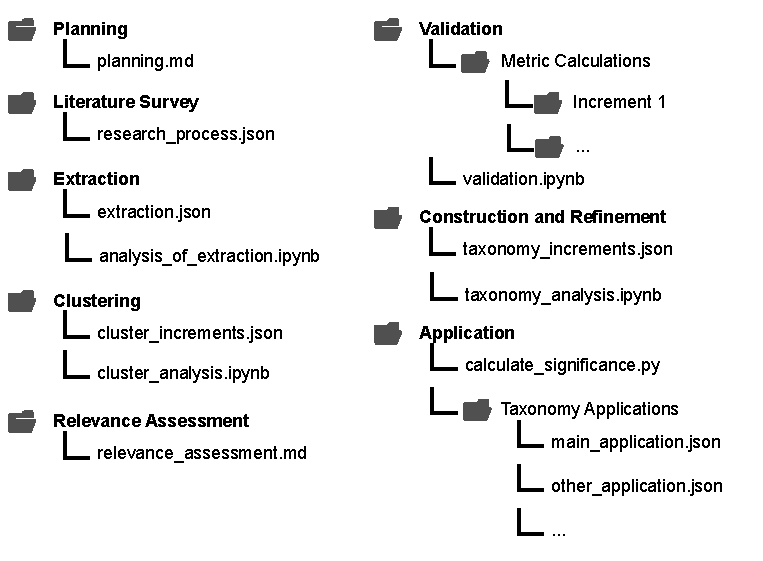
\includegraphics[width=0.7\linewidth]{figures/question_catalog/taxonomy-taxonomy_artifacts.drawio.pdf}
    \caption[Taxonomy Construction Artifacts]{Provided artifacts to support the taxonomy construction.}
    \label{fig:taxonomy_construction_artifacts}
\end{figure}

To facilitate the practical implementation of the taxonomy construction process, we provide a set of supporting artifacts, illustrated in \autoref{fig:taxonomy_construction_artifacts}, which are available in our replication package \cite{schneider_replication_2025}.

The provided artifacts are organized according to the corresponding phases of the construction process. For each phase, practitioners can access structured JSON files and Jupyter Notebooks that enable systematic execution of the process steps, comprehensive analysis of results, and calculation of relevant metrics. In addition, a usage guide is included in the replication package, offering instructions for leveraging these artifacts effectively throughout the taxonomy construction and evaluation workflow.

\section{Limitations}
\label{sec:tax_proce_limitations}

In this section, we acknowledge several limitations of our proposed taxonomy construction approach. 

First, several phases involve manual effort and qualitative judgments, which can introduce subjectivity and potentially affect reproducibility. For example, the extraction of classes, the deduplication and categorization steps within the \textsc{Clustering} phase, and the \textsc{Relevance Assessment} depend on human interpretation and the definition of the guiding criteria. The iterative nature of refinement also relies on judgments regarding when a satisfactory state is achieved, which can influence the overall duration and outcome of the process.

Second, the effectiveness of the \textsc{Application} phase as a final validation step is dependent on the selection and diversity of the use cases. If the chosen scenarios do not adequately represent the intended scope of the taxonomy, some of its deficiencies might not be identified. As a consequence, the generalizability of the validation results from this phase is tied to the representativeness of these application instances.

Finally, the initialization of the taxonomy is based on a literature survey. This foundation means that the process is dependent on the availability, quality, and scope of the existing literature. The comprehensiveness and representativeness of the resulting taxonomy are therefore contingent upon the body of literature identified and processed. For example, if the literature in a specific domain is sparse, exhibits bias, or is of inconsistent quality, this will inevitably impact the foundation upon which the taxonomy is built. Furthermore, the selection of seed publications and the execution of searches using Google Scholar may introduce selection bias if not carefully considered and justified.

\chapter{KGQA Retrieval Taxonomy}
\label{ch:question_catalog}

This chapter presents the second primary contribution, \textbf{C2}, of this thesis: a taxonomy for the classification of questions relevant to \gls{kgqa} systems, specifically within the context of literature search tasks. The taxonomy categorizes questions based on characteristics such as operational requirements and structural complexity, which are key dimensions influencing the retrieval performance of \gls{kgqa} systems. Consequently, the taxonomy supports the generation of diverse question datasets, thereby facilitating a thorough assessment of \gls{kgqa} system retrieval capabilities across various question types.

The development of this taxonomy followed the construction process detailed in \autoref{ch:taxonomy_construction_approach}. Accordingly, this chapter is structured to mirror the distinct phases of that methodology. Section~\ref{sec:taxonomy_planning} begins by outlining the \textsc{Planning} phase, defining the objectives and intended applications of the taxonomy. The subsequent \textsc{Literature Survey} phase, documented in Section~\ref{sec:literature_Survey}, describes the identification and selection of relevant literature candidates. Section~\ref{sec:kgqa_extraction_of_classes} then details the \textsc{Extraction} of classes from these candidates, which are subsequently grouped during the \textsc{Clustering} phase presented in Section~\ref{sec:taxonomy_clustering}. Following this, Section~\ref{sec:relevance_of_clusters_analysis} documents the \textsc{Relevance Assessment} of these clusters. Based on this assessment, the initial taxonomy is constructed and refined as described in Section~\ref{sec:taxonomy_design_construction}. The resultant \gls{kgqa} retrieval taxonomy is presented in its final form in Section~\ref{sec:taxonomy_final}. Its practical utility is then demonstrated through an application in a \gls{swa} context in Section~\ref{sec:taxonomy_application}. Concluding the chapter, Section~\ref{sec:taxonomy_threats_to_validity} discusses the potential threats to validity associated with the construction of this specific taxonomy.



\section{Planning}
\label{sec:selection_planning}

This section documents the planning of the parameter selection process. We first describe the methodology that was applied to realize the process. Next, we explain why we chose the Recall and Hits@10 metrics for the selection. Following this, we describe the dataset that was applied and the \glspl{llm}. Then, we describe the preliminary pipeline steps that are implemented before we describe why we decided to omit the StructGPT and ToG \gls{kgqa} approaches.

\subsection{Methodology}
\label{sec:selection_planning_methodology}

To carry out this process, we apply the \gls{ofat} method to identify the best parameters according to the Recall and Hits@10 metrics. In this method, a base configuration is selected and then each factor is successively varied over its range while all other factors are kept constant \cite{montgomery_design_2017}. Consequently, we defined a base configuration and a range of parameter values for each \gls{kgqa} approach. Then, following the \gls{ofat} method, multiple run configurations have been created based on the base configuration and ranges to subsequently test them using a reduced version of the \gls{kgqa} dataset.


\subsection{Metrics for Selection}
\label{sec:selecting_tuning_metric}

To conduct the selection, metrics need to be chosen that allow us to determine whether a change in the value of a parameter is justified. For the selection process, we focused on retrieval performance rather than generation. This is because the generation of the answers depends on the retrieved contexts, which means that if the retriever cannot find the contexts that are relevant, it will not be able to generate an answer based on it. With regard to the choice of retrieval metrics, our primary metric is Recall, although we also use Hits@10 where needed. There are several reasons for these metrics, which we explain in the following:

First, when constructing the \gls{kgqa} datasets (see Section~\ref{sec:implementation_qa_dataset_generation}), we ensured that only those triples were designated as the ground truth for which the content required to answer the question is actually present. We deliberately omitted any intermediate triples that must be traversed to reach the target since they are not strictly necessary to answer the actual question. To illustrate, consider a question that is asking for the authors of a paper. The authors are stored in separate nodes that all connect to a root node named \emph{Authors List}. That root node serves only as a means to reach the author nodes and does not provide the information necessary to answer the question. In our preliminary tests, we observed that retrievers tend to include such intermediate nodes in their retrieved context. Furthermore, because answer generation occurs after context retrieval, these nodes could be helpful during answer generation by providing additional context to the \gls{llm}. Consequently, we chose not to penalize this behavior, which is consistent with using the Recall metric.

With regard to the Hits@10 metric, this metric allows us to understand whether the retriever ranks those contexts that are more relevant higher than those that are less relevant. For example, if the retriever includes intermediate triples in their output, the Hits@10 metric is still maximal if those triples that are actually relevant are higher on the list of outputs.

\subsection{Choosing a Graph Variant}
\label{sec:selection_planning_graph_variant}

In Section~\ref{sec:contribution_templates} we introduced four different graph variants for our experiments to test the robustness of \gls{kgqa} approaches. However, due to cost reasons, we were unable to run the parameter selection process (and experiments) on all four graph variants. We therefore decided on \hyperref[enum:gv1]{\textbf{GV1}} as we believe that it is the graph variant with the most realistic modeling for real-world scenarios. The reason for this is that long paths allow the relationships between information to be captured, which preserves crucial context. Furthermore, the content is distributed by concern, which allows for extensibility in the future.

\subsection{Using a Reduced KGQA Dataset}
\label{sec:selection_planning_reduced_qa}

In addition to only running the selection process on one graph variant as mentioned above, we used a reduced version of the label-based \gls{kgqa} dataset (for \hyperref[enum:gv1]{\textbf{GV1}}) during the selection process. As described in Section~\ref{sec:implementation_qa_dataset_generation}, the \gls{kgqa} datasets were created with respect to use cases and retrieval operations. Each question is also classified as either semi-typed or untyped. For almost any pairing of a use case with a retrieval operation, there are four corresponding pairs of questions and answers. When constructing the reduced dataset, we therefore selected one semi-typed question per combination to ensure that each question is representative of the larger dataset. We chose semi-typed over untyped questions, as we expected them to perform better, which is important when selecting parameters. Consequently, the reduced \gls{kgqa} dataset for graph variant \hyperref[enum:gv1]{\textbf{GV1}} contains a total of 44 questions.



% We created \textbf{GV1} in such a way that it provides continued value for future use. This means that it should be easy to read and extendable for future contexts. 

% We gathered the majority of our results using graph variant \hyperref[enum:gv1]{\textbf{GV1}} as we expect \hyperref[enum:gv1]{\textbf{GV1}} to be the most relevant model for real-world scenarios due to its inherent extendability and its capability to capture semantic relationships. We explicitly state in each following section which graph variants we employed for the presented results.

\subsection{Large Language and Embedding Models}
\label{sec:selection_planning_llms}

As all retrievers are based on \glspl{llm}, the model selection is crucial for the performance of the retriever. Since HubLink, DiFaR, Mindmap, and FiDeLiS also work with embeddings, the selection of the embedding model is equally important.

For our experiments and the selection process, we implemented the following endpoints: \emph{OpenAI} as a proprietary provider as well as \emph{Ollama} and \emph{Hugging Face} for open-source models, both of which are run locally on the server. Furthermore, when choosing which models to use, we considered the following points:

\begin{enumerate}
    \item The OpenAI endpoint is proprietary and can introduce high costs if not managed carefully. As such, we considered the associated costs of the models and how many models from OpenAI we are using.
    \item Through testing, we found the Hugging Face models to be less optimized than the Ollama ones. This means that the amount of hardware memory resources required to run models on the Hugging Face endpoint is higher than on the Ollama endpoint, which may lead to \emph{out-of-memory} errors.
    \item We are restricted to the hardware resources available on our server. We have $32 GB$ of GPU memory available, which is enough to fit optimized \glspl{llm} of the size of $32B$ parameters on the GPU. However, running embedding models in parallel is then not feasible. Moreover, even if a large model fits on the GPU, its response time is likely too slow to be used in our experiments. Consequently, we chose to use smaller models. 
\end{enumerate}

To help in the selection process, we reviewed popular leaderboards to assess the performance of the models available. We examined two leaderboards, both reflecting the status as of February 16, 2025. For \glspl{llm}, we examined the \emph{Chatbot Arena Leaderboard}\footnote{\url{https://huggingface.co/spaces/lmarena-ai/chatbot-arena-leaderboard} [last accessed on 16.02.2025]}, proposed by \textcite{chiang_chatbot_2024}. For embedding models, we observed the \emph{Massive Multilingual Text Embedding Benchmark (MMTEB)}\footnote{\url{https://huggingface.co/spaces/mteb/leaderboard} [last accessed on 16.02.2025]}, introduced by \textcite{enevoldsen_mmteb_2025}. A snapshot of both leaderboards at the time of review is available in our replication package \cite{schneider_replication_2025}.

\subsubsection{Selection of LLMs}

We selected the following \glspl{llm} for our experiments: \emph{GPT-4o}, because the model is ranked at the highest position in the Chatbot Arena leaderboard via the OpenAI endpoint. \emph{GPT-4o-mini}, ranked 24th yet delivering a strong performance at a fraction of the cost and also \emph{O3-mini}, a newly released model that inherently implements chain-of-thought reasoning \cite{wei_chain--thought_2023}. To include open-source options, we chose \emph{Qwen2.5}, which is the Ollama endpoint model that performs the best on the leaderboard. However, due to our hardware constraints, we had to reduce the model to its $14B$ parameter variant. Furthermore, we selected \emph{Llama3.1}, which represents the second-best Ollama model in the leaderboard. However, we had to scale it down to the $8B$ parameter model because of hardware constraints. We also evaluated \emph{DeepSeek-R1} \cite{deepseek-ai_deepseek-r1_2025}, a new open-source reasoning model with promising benchmarks, but its performance-to-runtime ratio was substantially worse than that of our selected models, so we excluded it.

\subsubsection{Selection of Embedding Models} 

For embedding models, we included \emph{text-embedding-3-large}, the largest embedding model available via the OpenAI API. With regard to open-source models, we chose the \emph{Mxbai-Embed-Large} model, which is a fast and popular open-source model ranked 41st on the MMTEB leaderboard. Because it has a quick response time with good performance, it is a good choice for the base configurations in our selection process. We also evaluated \emph{Granite-Embedding}, a new Ollama endpoint model that is not yet on the leaderboard. Still, it is a promising model that is fast and looks to have a good performance. Finally, we tested \emph{gte-Qwen2-7B-instruct}, the top-ranked MMTEB model, but it exhibited slow inference and unexpectedly poor performance. We are not entirely sure why the performance of the model was poor, but we suspect that it may be due to the fact that it was used over the Hugging Face endpoint, which uses unoptimized models. Ollama, on the other hand, provides expert optimization for their models, which makes them faster and could make them perform better. This is the reason we opted to use models from Ollama over those provided on Hugging Face.

\subsection{Pre-, Post-Retrieval and Generation}
\label{sec:selection_planning_steps}

Our \gls{rag} pipeline involves four steps: 1) Pre-Retrieval, 2) Retrieval, 3) Post-Retrieval, and 4) Generation. In the following, we are going to introduce each step and its relevance to the parameter selection process.

\paragraph{Pre-Retrieval:} The pre-retrieval step is responsible for the preprocessing of the input question. We implemented a question augmentation technique that prompts an \gls{llm} to improve the given question by clarifying ambiguities, incorporating related keywords or phrases that will help the retrieval system retrieve more accurate and comprehensive information, and adding nouns or noun phrases to terms to clearly indicate their types or roles. Regarding the parameter selection, we tested each retriever with and without augmentation.

\paragraph{Retrieval:} The retrieval step is where both HubLink and the \gls{kgqa} baseline retrievers are applied. Each \gls{kgqa} approach has its own set of parameters relevant to the parameter selection process. For each parameter, we chose a range of values that were tested. The ranges are documented for each approach in the following sections.

\paragraph{Post-Retrieval:} In the post-retrieval step, the retrieved context from the previous step is processed. We implemented a function that prompts an \gls{llm} to rerank the retrieved contexts based on the provided question. During the parameter selection process, we then tested each \gls{kgqa} approach with and without reranking.

\paragraph{Generation:} The generation step is responsible for generating the final answer based on the question and the contexts that have been retrieved. The generation is done by prompting an \gls{llm} with the question and the contexts and asking it to generate an answer. However, because almost all \gls{kgqa} approaches provide an answer as part of their procedure, the generation step is skipped to retain the original answer of the approach. The only exception is \gls{difar}, for which generation prompting is used.

\textit{We provide the prompts that have been used for the question augmentation, reranking, and generation procedures in Appendix \ref{sec:appendix:prompts}.}

\subsection{Omitting StructGPT and ToG}
\label{sec:selection_planning_omitted_retrievers}

The use of the StructGPT \cite{jiang_structgpt_2023} and ToG \cite{sun_think--graph_2024} \gls{kgqa} approaches proved to be unsuitable in our experimental setting. Both approaches were unable to retrieve any relevant information from the graph, which is why we omitted them from the selection process and the experiments. A more detailed analysis of why these approaches are unable to answer the questions in our experiment can be found in Section~\ref{sec:discussion_on_evaluation_results}. 

\section{Literature Survey}
\label{sec:literature_Survey}

In this section, we document the literature survey that was conducted as part of the taxonomy development. A total of two iterations were performed to collect relevant candidate papers.

In the following, we start by defining the inclusion and exclusion criteria that have been specified to guide the assessment of relevance for paper candidates. Then, we describe the first iteration of the literature survey. Next, we outline the Google Scholar search that was carried out to find additional paper candidates. Finally, we detail the second iteration of the literature survey.


\subsubsection{Inclusion and Exclusion Criteria}
Following the advice of the construction approach in Section~\ref{sec:tax_con_literature_survey}, we define the following \emph{inclusion} and \emph{exclusion} criteria to assess the relevance of papers during the survey:

\paragraph{Inclusion Criteria}
\begin{itemize}
    \item Publications that directly or indirectly propose classes for the classification of questions.
\end{itemize}

\paragraph{Exclusion Criteria}
\begin{itemize}
    \item Publications for which the full text is not available.
    \item Publications that do not contain information on classes for the classification of questions.
    \item Publications that are not written in English.
\end{itemize}

In the following, we outline the two search iterations that were carried out. The search was stopped after two iterations in order to keep the scope of the thesis manageable. We also believe that, by the end of the second iteration, we had exhausted the pool of interesting information reachable from the seed papers and the applied search queries. This is supported by the fact that only 22 candidates are considered for a third iteration, which is noticeably lower than the 46 candidates examined during the second iteration. Therefore, if future work is interested in the continuation of the research, we recommend adding more search queries to increase the number of candidates. This continuation can be carried out seamlessly by utilizing our prepared artifacts in the replication package \cite{schneider_replication_2025}.

\subsection{First Literature Survey Iteration}

We populated the initial \emph{intermediate list} $\mathcal{L}_1$ with 11 publications provided by the thesis supervisor. After reviewing each paper, five publications have been excluded for not meeting the inclusion criteria or for not complying with the exclusion criteria. Through processing of the references and citations of the remaining papers, we added 19 papers to $\mathcal{L}_2$ and a total of six publications to the \emph{final list} $\mathcal{F}$. 

Looking at the relevant publications, some focus on the creation of \gls{qa} classifiers. \textcite{li_learning_2002} define a two-layered hierarchical taxonomy of question types in an open-domain context and learn a hierarchical question classifier based on this taxonomy. In addition, \textcite{singhal_att_1999} present a \gls{qa} system based on a taxonomy of question types. 

Instead of creating \gls{qa} classifiers, other publications focus on the creation of \gls{kgqa} datasets. \textcite{auer_sciqa_2023} present a scientific \gls{kgqa} dataset that has been created based on the \gls{orkg}. The dataset focuses on scholarly questions and includes a variety of types for the classification of questions. Furthermore, \textcite{karras_divide_2023} present a dataset of competency questions for the \gls{orkg}. Although they do not provide a question taxonomy explicitly in their paper, we extracted the question types from these instantiated questions.

Specifically in the domain of \gls{se}, \textcite{shaw_writing_2003} describes key components and considerations necessary to write effective research articles, which also include classes specifically suited for research questions. Furthermore, \textcite[287-290]{easterbrook_selecting_2008} provide a comprehensive guide for selecting empirical research methods in \gls{se}. Their work includes a categorization of the kinds of research question asked in \gls{se}.

\subsection{Search for Additional Relevant Paper Candidates}

To find additional sources of information and avoid clustering around a single topic, we conducted a search on Google Scholar after the first iteration. Our intention with this search was to find papers that were not already covered by the seed papers, meaning that they have not already been added in the lists $\mathcal{L}_1$ or $\mathcal{F}$. The search was carried out using the following search queries, which we chose based on the objective that we defined in the planning phase:

\begin{enumerate}[label=\textbf{Q\arabic*:}, leftmargin=5em]
    \item \enquote{research questions} AND \enquote{classification} OR \enquote{taxonomy} OR \enquote{types}
    \item \enquote{questions} AND \enquote{classification} OR \enquote{taxonomy} OR \enquote{types}
    \item \enquote{research questions} AND \enquote{construction} OR \enquote{development} OR \enquote{formulation}
    \item \enquote{question} AND \enquote{construction} OR \enquote{development} OR \enquote{formulation}
    \item \enquote{software engineering} AND \enquote{research questions} OR \enquote{classification} OR \enquote{taxonomy}
    \item \enquote{question answering} AND \enquote{classification} OR \enquote{taxonomy} OR \enquote{types}
    \item \enquote{question answering} AND \enquote{datasets} AND \enquote{graph}
    \item \enquote{question answering} AND \enquote{scholarly} AND \enquote{graph}
    \item \enquote{question answering} AND \enquote{structure}
\end{enumerate}

For each query, we looked at the first 40 results that have been returned sorted by relevance. The full search process that details each paper that was added by the search queries is available in our replication package \cite{schneider_replication_2025}. In the following, we provide an overview of the query results.

The first query \textbf{Q1} returned 3,620,000 results, from which we added four new candidates to $\mathcal{L}_2$. \textbf{Q2} returned 6,560,000 results. Although some publications looked interesting on the basis of their titles and abstracts, their full texts were not available. The next query \textbf{Q3} had 2,960,000 results from which we added four more candidates. Query \textbf{Q4} returned 4,560,000 results, but we excluded each paper through the application of our inclusion and exclusion criteria. Next, \textbf{Q5} returned 1,240,000 results, from which we added five publications to $\mathcal{L}_2$. In addition, one paper was found through the query that was already added to $\mathcal{L}_1$. The following query \textbf{Q6} returned 308,000 results, from which one paper was already considered in our candidates, and four more papers were added. The next query \textbf{Q7} had 76,900 results from which one paper was already considered and three more were added. Query \textbf{Q8} had the least number of results, with 5,040 papers returned, but the most relevant papers to our cause. We added three more papers to our candidates for the next iteration. Eight papers that the query returned were already in $\mathcal{L}_1$, $\mathcal{L}_2$ or $\mathcal{F}$. Finally, \textbf{Q9} had 196,000 results, from which we added four more candidates to our list. One of the returned papers was already on our list. In summary, a total of 28 new publications were added to $\mathcal{L}_2$ based on these searches.

\subsection{Second Literature Survey Iteration}

The second iteration started with a total of 47 papers in $\mathcal{L}_2$. After processing each paper, we added 23 publications to $\mathcal{L}_3$ for the next iteration. Furthermore, we added 21 papers to the final list $\mathcal{F}$.

% Dataset Papers
Several of the new papers added to $\mathcal{F}$ propose new datasets or benchmarks for \gls{kgqa}. \textcite{dubey_lc-quad_2019} introduce LC-QuAD, which is a large dataset of natural language questions with paraphrases along with corresponding SPARQL queries for Wikidata and DBpedia. In their work, they specifically provide a taxonomy of classes for question classification. In addition, \textcite{bordes_large-scale_2015} present the SimpleQuestions dataset, which is specifically designed for single-fact retrieval. Although they provide minimal information on question types in their work, we were able to identify some classes. \textcite{tran_comparative_2022} developed COVID-KGQA, which is a multilingual corpus related to COVID. In their work, they also evaluated the influence of a \enquote{Wh}-based question taxonomy on the performance of their dataset. \textcite{usbeck_qald-10_2023} add another \gls{kgqa} dataset with QALD-10, which is a \gls{qa} benchmarking dataset. They provide some information about the types of questions that are included in the dataset. Furthermore, \textcite{banerjee_dblp-quad_2023} created the DBLP-Quad dataset which is focused on scholarly questions. Their work also provides a taxonomy that describes the types of question that the dataset consists of. Another dataset is Hybrid-SQuAD, which has been designed to address scholarly \gls{qa} by \textcite{taffa_hybrid-squad_2024}. In addition, \textcite{jaradeh_question_2020} present a BERT-based \gls{qa} system for tabular representations in \gls{orkg}, together with the ORKG-QA benchmark, a small dataset of scholarly questions. \textcite{steinmetz_what_2021} survey the challenges for \gls{kgqa} datasets and extract the answer types from these.

% Classifier Papers
Beyond the datasets themselves, several studies focus on creating classifier models with the task of classifying questions. \textcite{bolotova_non-factoid_2022} provide a systematic categorization of non-factoid questions and their corresponding answer structures intended for open-domain \gls{qa} systems. \textcite{liu_taxonomy_2015} similarly propose a taxonomy for classifying questions on social networks such as Twitter. Furthermore, \textcite{moldovan_structure_2000} provide a comprehensive taxonomy for open-domain \gls{qa} that integrates both syntactic and semantic techniques, while \textcite{riloff_rule-based_2000} discuss a rule-based system for reading comprehension and illustrate how hand-crafted rules depend on distinct question types. Furthermore, \textcite{nguyen_ripple_2017} propose an ontology-based \gls{qa} system for the Vietnamese language, including question structures as part of their work. \textcite{chernov_linguistically_2015} describe a question interpretation module for a dialogue-based quiz \gls{qa} application.

% Research Question Papers
Another set of publications examines how to classify or formulate research questions. \textcite{dillon_classification_1984} investigates the classification of research questions as suggested by Aristotle. \textcite{ratan_formulation_2019}  emphasize how a well-structured research question facilitates effective scholarly work. In addition, \textcite{kamper_types_2020} discusses the importance of well-defined research questions in the field of healthcare. They provide and discuss a small taxonomy of question types. \textcite{sjoberg_future_2007} propose a taxonomy of archetype classes for \gls{se} research, suggesting a foundational framework for shaping and guiding empirical studies.

% Other
Other papers focus on the design and evaluation of \gls{qa} systems. \textcite{allam_question_2016} provide an overarching view of \gls{qa} and its core components, revealing how the types of questions factor into the architecture of the system. A more conceptual approach is seen in \textcite{mikhailian_learning_2009}, who introduce the ideas of Asking Point and Expected Answer Type as guiding concepts to capture the intent of the question. 

\section{Extraction of Classes}
\label{sec:kgqa_extraction_of_classes}

A total of 81 publications were considered in our literature survey in the first ($\mathcal{L}_1$) and second ($\mathcal{L}_2$) iterations. Among these publications, 27 were selected as sources for class extraction ($\mathcal{F}$). After the search, we performed a manual extraction of the classes. A total of 227 classes were extracted from these publications. 

In the following sections, we analyze the distribution of the classes and publications from which the classes have been extracted. We first look at the distribution of the classes by the category and domain of the publication. Subsequently, we analyze the publication years prior to evaluating the citations and references among the papers.

\subsection{Distribution of Classes by Category and Domain}

\begin{table}[t]
    \centering
    \begin{tabular}{l l r r}
        \toprule
        \textbf{Category} & \textbf{Domain} & \textbf{Classes} & \textbf{Papers} \\
        \midrule
        KGQA Dataset & General & 27 & 4 \\
        KGQA Dataset & Requirements Engineering & 3 & 1 \\
        KGQA Dataset & Scholarly & 38 & 4 \\
        KGQA Dataset & Covid & 9 & 1 \\
        Question Classifier & General & 58 & 6 \\
        Question Classifier & Social Science & 4 & 1 \\
        Question Classifier & Spoken NLP & 8 & 1 \\
        Question Classifier & Vietnamese Language & 22 & 1 \\
        Research Questions & General & 12 & 2 \\
        Research Questions & Design Science & 10 & 1 \\
        Research Questions & Software Engineering & 21 & 2 \\
        Research Questions & Healthcare & 3 & 1 \\
        Other & General & 8 & 1 \\
        Other & Software Engineering & 4 & 1 \\
        Total & & 227 & 27 \\
        \bottomrule
    \end{tabular}
    \caption[Distribution of Classes by Paper Category and Domain]{Distribution of the extracted classes by the papers they were extracted from.}
    \label{table:question_type_distribution}
\end{table}

During the search, we assigned each paper to one of the categories introduced in the planning step. If a paper could not be clearly classified into any of the predefined categories, we added it to the category \emph{Other}. Furthermore, each publication was assigned a domain to understand its scope. 

\autoref{table:question_type_distribution} shows the distribution of the publications and extracted classes based on these categories and domains. The table illustrates that most of the question classes come from the category \emph{Question Classifier}, which includes those publications that propose methods to classify questions. This category comprises 92 question classes sourced from nine publications in four domains. Most of the papers in this category fall into the General domain, which means that their classifications are not limited to a specific topic area. Each of the remaining domains in this category (Social Science, Spoken NLP, Vietnamese Language) is represented by only a single paper. It is logical that this category includes the largest number of classes, as considering question structure and types is crucial when building classifiers. The classes extracted from these papers primarily relate to a form of answer type in which the expected format and content of the answer are considered, and the types of questions, which reflects the data processing required to derive an answer.

The second largest category by number of extracted classes is the \emph{\gls{kgqa} Dataset} category (77 classes from 10 papers). This category includes papers that propose a dataset for \gls{kgqa} and is represented by four domains, where the General domain and the Scholarly domain are equally represented by four papers each. The other two domains covered are Requirements Engineering, and one paper related to Covid. In general, this category provides critical insights relevant when working with \glspl{kg}. The literature suggests considering the structure of the \gls{kg} when classifying questions, which can indicate the complexity of the retrieval task. Additionally, considering the required \gls{kg} operations is relevant for understanding processing needs.

The third most common category is \emph{Research Questions}, which includes publications focused on the formulation and structure of research questions. Represented by six papers, this category includes 46 extracted question classes from four different domains. The General and Software Engineering domains are equally represented, each with two papers. The other two domains are related to Design Science and Healthcare. Generally, this category is useful for understanding the needs of researchers, which is particularly important for our taxonomy. As such, the literature highlights the importance of considering the focus of a question and its intended goal.

Finally, the \emph{Other} category includes publications that did not fit the predefined categories. This category is represented by two papers and includes 12 extracted question classes. The domains of these papers are Software Engineering and the General domain.

\subsection{Distribution of Publications by Year}

\begin{figure}[t]
    \centering
    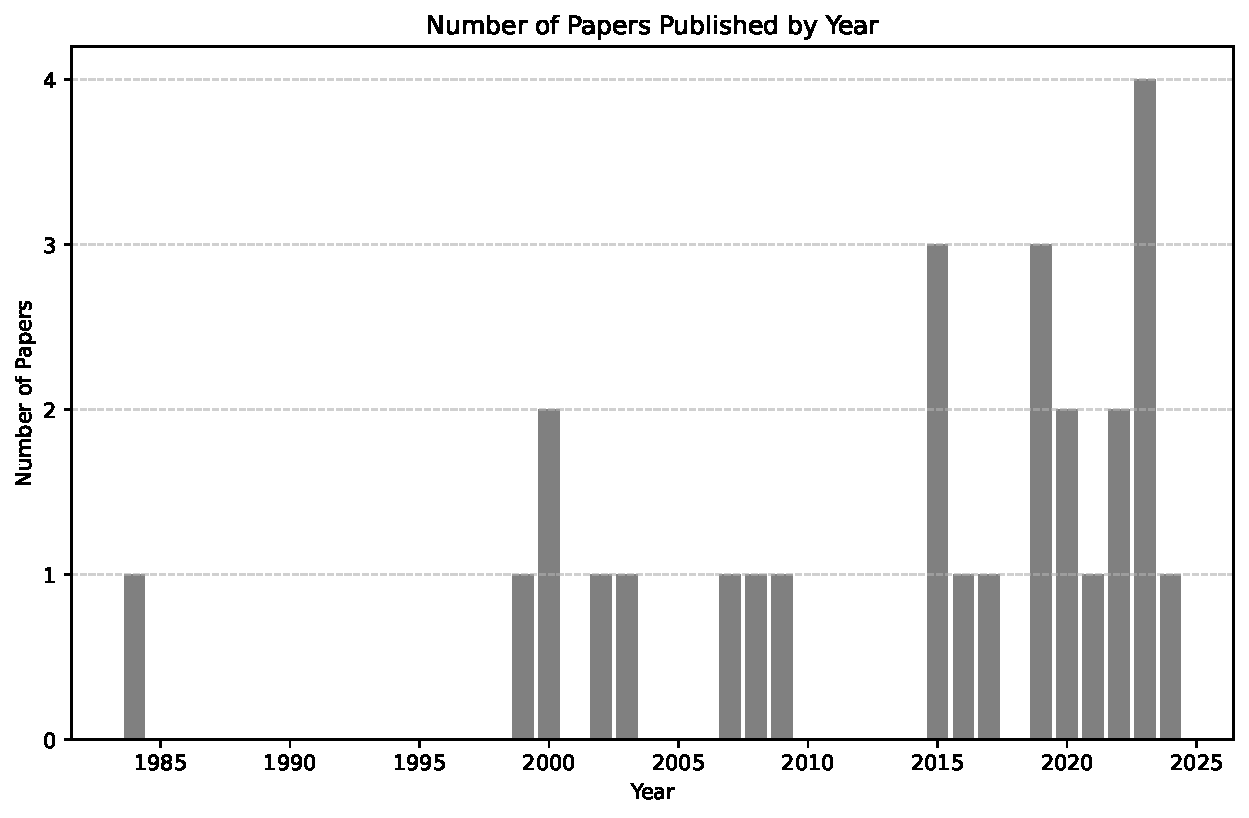
\includegraphics[width=0.99\textwidth]{figures/question_catalog/papers_by_year.pdf}
    \caption[Distribution of Papers by Publication Year]{The distribution of papers by their year of publication.}
    \label{fig:papers_by_year}
\end{figure}

\autoref{fig:papers_by_year} shows the distribution by publication year for the papers from which we extracted classes. The years range from 1984 to 2024, with most publications published in the last decade. The oldest paper is authored by \textcite{dillon_classification_1984}, who investigated the classification of research questions as suggested by Aristotle. The most recent paper is authored by \textcite{taffa_hybrid-squad_2024}, which presents the Hybrid-SQuAD dataset designed to address scholarly \gls{qa} by combining tabular and textual data. The year 2023 yielded the most publications in our set (four papers), while other years contributed between one and three papers. Several years within the range had no publications matching our criteria.



\subsection{Distribution of Citations and References}

\begin{table}[t]
    \centering
    \begin{minipage}[t]{0.43\textwidth}
        \centering
        \begin{tabular}{l c}
            \toprule
            \textbf{Paper} & \textbf{Number of Citations} \\
            \midrule
            \cite{li_learning_2002} & \cite{auer_sciqa_2023}, \cite{bolotova_non-factoid_2022}, \cite{allam_question_2016}, \cite{chernov_linguistically_2015} \\
            \cite{dubey_lc-quad_2019} & \cite{auer_sciqa_2023}, \cite{usbeck_qald-10_2023}, \cite{banerjee_dblp-quad_2023} \\
            \cite{singhal_att_1999} & \cite{auer_sciqa_2023}, \cite{chernov_linguistically_2015} \\
            \cite{mikhailian_learning_2009} & \cite{auer_sciqa_2023}, \cite{chernov_linguistically_2015} \\
            \cite{auer_sciqa_2023} & \cite{karras_divide_2023}, \cite{taffa_hybrid-squad_2024} \\
            \cite{jaradeh_question_2020} & \cite{karras_divide_2023}, \cite{taffa_hybrid-squad_2024} \\
            \cite{bordes_large-scale_2015} & \cite{auer_sciqa_2023} \\
            \cite{riloff_rule-based_2000} & \cite{auer_sciqa_2023} \\
            \cite{sjoberg_future_2007} & \cite{karras_divide_2023} \\
            \cite{moldovan_structure_2000} & \cite{chernov_linguistically_2015} \\
            \cite{banerjee_dblp-quad_2023} & \cite{taffa_hybrid-squad_2024} \\
            \bottomrule
        \end{tabular}
        \caption[Number of Citations within Paper Selection]{The number of times a paper has been cited by another paper within $\mathcal{F}$.}
        \label{table:papers_by_citations}
    \end{minipage}
    \hfill
    \begin{minipage}[t]{0.55\textwidth}
        \centering
        \begin{tabular}{l c}
            \toprule
            \textbf{Paper} & \textbf{References} \\
            \midrule
            \cite{auer_sciqa_2023} & \cite{bordes_large-scale_2015}, \cite{dubey_lc-quad_2019}, \cite{li_learning_2002}, \cite{singhal_att_1999}, \cite{riloff_rule-based_2000}, \cite{mikhailian_learning_2009} \\
            \cite{chernov_linguistically_2015} & \cite{singhal_att_1999}, \cite{moldovan_structure_2000}, \cite{mikhailian_learning_2009}\\
            \cite{karras_divide_2023} & \cite{sjoberg_future_2007}, \cite{auer_sciqa_2023}, \cite{jaradeh_question_2020} \\
            \cite{taffa_hybrid-squad_2024} & \cite{auer_sciqa_2023}, \cite{banerjee_dblp-quad_2023}, \cite{jaradeh_question_2020} \\
            \cite{bolotova_non-factoid_2022} & \cite{li_learning_2002} \\
            \cite{allam_question_2016} & \cite{li_learning_2002} \\
            \cite{banerjee_dblp-quad_2023} & \cite{dubey_lc-quad_2019} \\
            \cite{usbeck_qald-10_2023} & \cite{dubey_lc-quad_2019} \\
            \bottomrule
        \end{tabular}
        \caption[Number of References within Paper Selection]{The number of times a paper has referenced another paper within $\mathcal{F}$.}
        \label{table:papers_by_references}
    \end{minipage}
\end{table}


\autoref{table:papers_by_citations} illustrates the frequency with which the papers in our selected set ($\mathcal{F}$) cite each other. This provides insight into the relative influence of each publication within our selection. In particular, \cite{li_learning_2002} is the most frequently cited paper, indicating a potentially greater influence within our selected set of papers. In addition, five papers are cited twice and five are cited once, suggesting a modest influence within the set. Of the 27 papers in the final list, 16 were not cited by any other paper within this set, suggesting that they have had limited direct influence on the classification schemes developed in the cited works within our collection.

In contrast, \autoref{table:papers_by_references} details how often each paper references other publications within our selection. This data reveals the extent to which the classifications may have been informed by prior work. According to the data, \cite{auer_sciqa_2023} stands out with six references, indicating that its classifications are heavily influenced by other publications on our list. Similarly, \cite{chernov_linguistically_2015} references four papers, while both \cite{karras_divide_2023} and \cite{taffa_hybrid-squad_2024} cite three publications each. In addition, four papers \cite{bolotova_non-factoid_2022,allam_question_2016,banerjee_dblp-quad_2023,usbeck_qald-10_2023} include only one reference. Overall, with only eight out of 27 papers referencing other works in the data, it appears that most of the publications derive their insights independently.


\section{Clustering of Extracted Classes}
\label{sec:taxonomy_clustering}

After extracting 227 classes for question classification, we performed the \textsc{Clustering} phase of the taxonomy construction process. The goal of the clustering process is to semantically group classes with similar names or descriptions and to merge duplicate classes proposed by multiple publications, thereby providing an overview of the unique classes and reducing redundancy. The clustering process is carried out in two steps: \emph{Deduplication} and \emph{Categorization}, as described in Section~\ref{sec:tax_proc_clustering}.

\subsection{Deduplication Process}
In the first step, the names of the question classification classes and the descriptions provided by the respective authors were manually analyzed for similarities. All classes $\mathcal{C}$ that shared a similar or identical name and had semantically similar descriptions were grouped together. After performing this process, the 227 classes in $\mathcal{C}$ were consolidated into 96 merged classes $\hat{\mathcal{C}}$. Each merged class was then given a unique name and description by combining the names and descriptions of the classes within it.

\subsection{Categorization Process}
In the second step, we clustered the classes $\hat{\mathcal{C}}$ into categories. For this purpose, we analyzed the names and descriptions of the groups to identify commonalities. Classes that exhibited coherence were grouped into a category, resulting in a total of nine categories. Finally, based on the combined names and descriptions of the classes $\hat{\mathcal{C}}$ within the categories, we established a unique name and description for each of the categories. The detailed process is documented in our replication package \cite{schneider_replication_2025}. An overview of each category and its metadata is shown in \autoref{table:clustering_result}. In the following, we present the final categories with their names, descriptions, and characteristics.

\label{enum:cluster_1}
\paragraph{Category 1} We identified that the classes in this category are about the representation of knowledge in a \gls{kg}. It describes the granularity of the facts that the retriever needs to retrieve in order to arrive at the answer. The cluster distinguishes between two classes. First, questions that require the retrieval of multiple facts from the graph to be answered. Second, questions that require only one fact. As such, we named this category \emph{Graph Representation}. Five sources form this cluster \cite{banerjee_dblp-quad_2023,auer_sciqa_2023,dubey_lc-quad_2019,jaradeh_question_2020,bordes_large-scale_2015}. From the categories of these papers we can conclude that they originate from the development of \gls{kgqa} datasets, with most contributions emerging in the last five years. Moreover, the contributions span both the academic and general domains, suggesting a broad applicability of this distinction. 

\label{enum:cluster_2}
\paragraph{Category 2} This category contains the largest number of classes among all categories, encompassing a total of 33 classes derived from 25 different publication sources \cite{allam_question_2016,moldovan_structure_2000,steinmetz_what_2021,singhal_att_1999, dillon_classification_1984,riloff_rule-based_2000,taffa_hybrid-squad_2024,mikhailian_learning_2009,sjoberg_future_2007, nguyen_ripple_2017,chernov_linguistically_2015,li_learning_2002, shaw_writing_2003,bolotova_non-factoid_2022,banerjee_dblp-quad_2023,auer_sciqa_2023,dubey_lc-quad_2019,jaradeh_question_2020,tran_comparative_2022,easterbrook_selecting_2008,ratan_formulation_2019,kamper_types_2020,liu_taxonomy_2015,karras_divide_2023,thuan_construction_2019}. Each class categorizes a question based on the expected format and content of its answer. These classes span a wide range, including \emph{entities}, \emph{names}, \emph{dates}, \emph{monetary values}, and \emph{bibliometric numbers}. We find that some classes are addressed by multiple sources. The \emph{boolean} class is the most widely considered, appearing in 10 sources. This is followed by the Human/Person, Location, and Quantitative classes, each appearing in seven sources. The classes \emph{date} and \emph{description} are also commonly represented, with five sources each. Additionally, the classes \emph{undefined}, \emph{time}, \emph{organization}, and \emph{entity} are mentioned in four sources each. The remaining classes are referenced less frequently. Overall, we named this category \emph{answer type}.

\label{enum:cluster_3}
\paragraph{Category 3} This category consists of classes that define the types of operations a retriever must perform to arrive at an answer, such as \emph{negation}, \emph{contingencies}, \emph{counting}, and \emph{comparison}. With contributions from 17 different sources \cite{allam_question_2016,sjoberg_future_2007,banerjee_dblp-quad_2023,auer_sciqa_2023,nguyen_ripple_2017,easterbrook_selecting_2008,dillon_classification_1984, ratan_formulation_2019,kamper_types_2020,dubey_lc-quad_2019,usbeck_qald-10_2023,steinmetz_what_2021,tran_comparative_2022,bolotova_non-factoid_2022,jaradeh_question_2020,bordes_large-scale_2015,karras_divide_2023}, it is the second most prevalent cluster identified in our extraction. The majority of these sources stem from the \gls{kgqa} dataset literature, although the category is also addressed in works on question classification and in studies focused on scholarly research questions. It is primarily considered within open-domain and academic contexts but also receives attention in the software engineering domain. In addition, specialized fields such as requirements engineering and Covid-related research contribute to this category. We refer to this category as \emph{Question Types}.


\begin{sidewaystable}[p]
    \centering
    \resizebox{\textwidth}{!}{
    \begin{tabularx}{\textwidth}{p{4cm} p{1.5cm} p{1.5cm} X X X}     
        \toprule
        \textbf{Category Name} & \textbf{Classes} & \textbf{Sources} & \textbf{Domains} & \textbf{Years} & \textbf{Source Categories} \\
        \midrule
        Graph Representation & 2 & 5 & Scholarly, Open & 2015, 2019, 2020, 2023 & KGQA Dataset \\
        Answer Type & 33 & 25 & Scholarly, Open, Software Engineering, Language specific, Spoken NLP, Covid, Healthcare, Social Science, Requirements Engineering, Design Science & 1984, 1999, 2000, 2002, 2003, 2007, 2008, 2009, 2015, 2016, 2017, 2019, 2020, 2021, 2022, 2023, 2024 & Question Classifier, KGQA Dataset, Research Questions, Other \\
        Question Types & 18 & 17 & Scholarly, Open, Software Engineering, Language specific, Healthcare, Covid, Requirements Engineering & 1984, 2007, 2015, 2016, 2017, 2019, 2020, 2021, 2022, 2023 & Question Classifier, KGQA Dataset, Research Questions, Other \\
        WH-Patterns & 9 & 5 & Scholarly, Open, Covid, Language specific & 2000, 2017, 2022, 2023 & Question Classifier, KGQA Dataset \\
        Specialized KB Types & 2 & 3 & Scholarly, Open & 2019, 2021, 2023 & KGQA Dataset \\
        Research Focus & 8 & 2 & Scholarly, Software Engineering & 2003, 2024 & KGQA Dataset, Research Questions \\
        Answer Credibility & 5 & 5 & Requirements Engineering, Social Science, Healthcare, Open & 1984, 2020, 2022, 2023 & KGQA Dataset, Question Classifier, Research Questions \\
        Question Goal & 7 & 7 & Software Engineering, Design Science, Open & 2000, 2003, 2008, 2016, 2019, 2022 & Research Questions, Question Classifier \\
        Application Specific & 12 & 5 & Design Science, Language specific, Spoken NLP, Open & 2000, 2015, 2017, 2019, 2021 & Research Questions, Question Classifier, KGQA Dataset \\
        \bottomrule
    \end{tabularx}
    }
    \caption[Clustering of Extracted Classes]{Clustering Results for the Extracted Question Types from the Literature}
    \label{table:clustering_result}
\end{sidewaystable}

\label{enum:cluster_4}
\paragraph{Category 4} This category groups questions based on their interrogative form, distinguishing between different \enquote{Wh} word patterns such as \emph{what}, \emph{where}, \emph{which}, \emph{when}, \emph{who}, \emph{why}, \emph{whose}, and \emph{whom}. It is rooted in early question classification research and continues to be relevant in current studies. The cluster is derived from five different sources \cite{auer_sciqa_2023,riloff_rule-based_2000,tran_comparative_2022,nguyen_ripple_2017,moldovan_structure_2000} and spans both scholarly and general domains, with additional contributions from specialized areas such as Covid-related research and studies focused on the Vietnamese language. We refer to this fourth category as \emph{WH-Patterns}.

\label{enum:cluster_5}
\paragraph{Category 5} We named this category \emph{Specialized Knowledge Base Types}, as it comprises question classes tailored to specific \glspl{kb}. These include classes related to \gls{orkg}, SPARQL queries, and Wikidata qualifiers. Consequently, such classifications are only applicable when the question is executed against the corresponding \gls{kb}. The category is supported by three recent sources \cite{auer_sciqa_2023,steinmetz_what_2021,dubey_lc-quad_2019}, spanning both scholarly and general domains. Notably, it is exclusively addressed within the context of \gls{kgqa} dataset literature.

\label{enum:cluster_6}
\paragraph{Category 6} We refer to the category as \emph{Research Focus} as it centers on classifying questions according to their research-related focus. It includes classes such as Research Output, Development Methods, and Modeling Approaches and is supported by only two publications. The first is \cite{taffa_hybrid-squad_2024}, a 2024 contribution in the \gls{kgqa} dataset category, which specifically targets scholarly content. The second is \cite{shaw_writing_2003}, a 2003 study centered on research questions within the software engineering domain.

\label{enum:cluster_7}
\paragraph{Category 7} We refer to this category as \emph{Answer Credibility}, as it classifies questions based on the perceived truthfulness or reliability of the expected answer. It includes classes such as \emph{factual}, \emph{opinion}, \emph{debate}, \emph{conversational}, and \emph{predictive}. This cluster is supported by five sources \cite{karras_divide_2023,bolotova_non-factoid_2022,liu_taxonomy_2015,dillon_classification_1984,kamper_types_2020}, spanning domains such as requirements engineering, social sciences, healthcare, and the open domain. Most sources are from recent years, with the earliest dating back to 1984. The category is considered in \gls{kgqa} dataset literature, question classification studies, and research focusing on scholarly questions.

\label{enum:cluster_8}
\paragraph{Category 8} We refer to the eighth category as \emph{Question Goal}, as it captures the overarching intent or purpose behind a question. It includes classes such as \emph{exploratory}, \emph{reasoning}, \emph{problem solving}, and \emph{gap spotting}. This category is supported by seven sources \cite{easterbrook_selecting_2008,thuan_construction_2019,ratan_formulation_2019,shaw_writing_2003,bolotova_non-factoid_2022,moldovan_structure_2000,allam_question_2016}, spanning domains such as software engineering, design science, and the open domain. The publication years range from 2000 to 2022, reflecting both foundational and more recent work. The category is primarily addressed in question classification studies and literature focused on research question formulation.

\label{enum:cluster_9}
\paragraph{Category 9} We refer to this category as \emph{Application Specific}, as it encompasses classes that are tailored to particular applications or use cases. These include categories such as Research Question Utilization, Research Question Typology, and Outcome Artifact Classification. The category is supported by five sources \cite{thuan_construction_2019,nguyen_ripple_2017,chernov_linguistically_2015,moldovan_structure_2000,steinmetz_what_2021}, spanning domains such as design science, Vietnamese language studies, spoken natural language processing, and the open domain. The publication years range from 2000 to 2021. This category is addressed in question classification studies, research question-focused literature, and \gls{kgqa} dataset research.

\section{Relevance Assessment of Clusters}
\label{sec:relevance_of_clusters_analysis}

In this section, we present the \textsc{Relevance Assessment} phase of the taxonomy construction approach. For each category presented in the prior Section~\ref{sec:taxonomy_clustering}, we discuss the relevance to the taxonomy. This assessment is based on the established name and description of the category to determine if it aligns with the goal of the taxonomy. In particular, a category is seen as relevant if each of the following questions hold true:

\begin{enumerate}[label=\textbf{GQ\arabic*.}, leftmargin=2.5em]
    \item Does the category capture characteristics of questions to test the capabilities of \gls{kgqa} retrieval systems, or does it reflect aspects specific to the scholarly literature search domain?
    \item Can the category be generalized across different \gls{kgqa} systems and within the literature search domain?
    \item Can the classes within the category inform and guide the construction of diverse and meaningful evaluation datasets?
\end{enumerate}

In the following, we assess each category towards the questions.

\hyperref[enum:cluster_1]{\textbf{Category 1 – Graph Representation}} \\
This category captures structural aspects of question complexity by distinguishing between questions that require the retrieval of single versus multiple facts. This distinction directly impacts the complexity of the retrieval process and is broadly applicable across \gls{kgqa} systems. Moreover, it is particularly relevant in the scholarly domain, where complex questions are common. The cluster also offers concrete guidance for the construction of datasets that vary in granularity with respect to graph traversal. \\
\textit{Relevant:} \textbf{Yes}

\hyperref[enum:cluster_2]{\textbf{Category 2 – Answer Type}} \\
This category categorizes questions by the expected type of answer, such as dates, entities, quantities, or boolean values. These categories are helpful in describing the characteristics of questions in a literature search to construct diverse datasets. Furthermore, they are broadly applicable across domains and \gls{kgqa} systems. \\
\textit{Relevant:} \textbf{Yes}

\hyperref[enum:cluster_3]{\textbf{Category 3 – Question Types}} \\
This category focuses on logical and computational operations implied by a question, such as comparison, counting, or negation. These operations are central in retrieval and directly relate to the functional requirements of a retriever. The cluster generalizes across domains and offers valuable guidance for the inclusion of questions targeting different retrieval abilities. \\
\textit{Relevant:} \textbf{Yes}

\hyperref[enum:cluster_4]{\textbf{Category 4 – WH-Patterns}} \\
Although WH-patterns are commonly used in question classification, they primarily reflect linguistic surface forms rather than the underlying retrieval characteristics. Furthermore, the classes are not general enough to provide meaningful characteristics in the scholarly literature search setting. Its utility for guiding the construction of a diverse dataset is also limited. While it may promote diversity with regard to WH-forms, it is not helpful to capture the meaning of questions or reliably correspond to distinct retrieval challenges. \\
\textit{Relevant:} \textbf{No}

\hyperref[enum:cluster_5]{\textbf{Category 5 – Specialized Knowledge Base Types}} \\
This category encompasses classes that are specific to certain knowledge bases, such as Wikidata qualifiers or ORKG-specific constructs. Although these distinctions are meaningful within their contexts, they do not generalize across \gls{kgqa} systems or domains. Consequently, the cluster offers limited value for constructing broadly applicable evaluation datasets and is more reflective of system-specific constraints than question-inherent properties. \\
\textit{Relevant:} \textbf{No}

\hyperref[enum:cluster_6]{\textbf{Category 6 – Research-Focus}} \\
This category categorizes questions based on their orientation towards research-related topics such as research methods or modeling approaches. Although the classes may be domain-specific, they align closely with our focus on scholarly literature search. In addition, the cluster is relevant for designing evaluation datasets that capture the diversity of scholarly questions. \\
\textit{Relevant:} \textbf{Yes}

\hyperref[enum:cluster_7]{\textbf{Category 7 – Answer Credibility}} \\
This category considers the credibility of expected answers, such as factual, predictive, or opinion-based. Because the literature search can include various credibility types, this classification is relevant to the scholarly literature search and generalizable across different domains. Moreover, considering this classification promotes diversity in the creation of question datasets. \\
\textit{Relevant:} \textbf{Yes} 

\hyperref[enum:cluster_8]{\textbf{Category 8 – Question Goal}} \\
This category addresses the underlying intent behind a question, such as problem solving, reasoning, or exploration. These types of goals are relevant for scholarly literature search to capture the intent behind the question. As such, it promotes diversity in question dataset creation. \\
\textit{Relevant:} \textbf{Yes}

\hyperref[enum:cluster_9]{\textbf{Category 9 – Application-Specific}} \\
This category includes classes that are defined in relation to specific applications or use contexts, such as outcome artifact classification or research question typologies. Although these categories may be useful within individual domains, they do not reflect generalizable properties of the questions themselves. \\
\textit{Relevant:} \textbf{No}

Based on the analysis of category relevance, we conclude that six out of a total of nine identified categories can be considered relevant. Each of these categories further comprises a number of classes. For each individual class, a relevance assessment was also performed, with the detailed results documented in our replication package \cite{schneider_replication_2025}. In total, 96 classes within the categories were examined, of which 58 were rated as relevant and 38 as not relevant. This yields a class-level relevance ratio of:

\[
\text{Relevance}_\text{classes} = \frac{|\text{relevant classes}|}{|\text{total classes}|} = \frac{58}{96} \approx 0.6
\]

This indicates that approximately 60\% of the classes extracted from the literature are considered relevant for our taxonomy. A similar pattern emerges at the category level. The relevance ratio for categories is given by

\[
\text{Relevance}_\text{categories} = \frac{|\text{relevant categories}|}{|\text{total categories}|} = \frac{6}{9} = \frac{2}{3} \approx 0.66
\]

This indicates that a substantial portion of the identified categories are meaningful for structuring our taxonomy.


\section{Taxonomy Construction and Refinement}
\label{sec:taxonomy_design_construction}

This section documents the \textsc{Taxonomy Construction and Refinement} phase of the taxonomy construction approach. The first increment of the taxonomy was initialized based on the relevant categories from Section~\ref{sec:relevance_of_clusters_analysis}. We then identified several shortcomings of the taxonomy, which led to two more refinement steps until we were satisfied with the result. In the following sections, we describe each of the three increments that led to the final \gls{kgqa} retrieval taxonomy.

\subsection{First Taxonomy Increment}

The following sections will introduce the construction and validation of the first taxonomy increment.

\begin{table}[t]
\centering
\resizebox{\textwidth}{!}{%
\begin{tabular}{|l|lll|}
\hline
\textbf{Category} & \multicolumn{3}{l|}{\textbf{Classes}} \\
\hline
\begin{tabular}[c]{@{}l@{}}Graph \\ Representation\end{tabular} & \multicolumn{2}{l|}{Single Fact} & Multi Fact \\
\hline
\multirow{11}{*}{Answer Type} & \multicolumn{1}{l|}{Undefined} & \multicolumn{1}{l|}{Date} & Tool/Notation \\ \cline{2-4} 
 & \multicolumn{1}{l|}{Definition} & \multicolumn{2}{l|}{Theoretical Framework} \\ \cline{2-4} 
 & \multicolumn{1}{l|}{Abbreviation} & \multicolumn{1}{l|}{Instructional} & \multicolumn{1}{l|}{Actor} \\ \cline{2-4} 
 & \multicolumn{1}{l|}{Boolean} & \multicolumn{1}{l|}{Entity} & Human/Person \\ \cline{2-4} 
 & \multicolumn{1}{l|}{Quantitative} & \multicolumn{1}{l|}{Solution} & Time \\ \cline{2-4} 
 & \multicolumn{1}{l|}{Title} & \multicolumn{1}{l|}{Monetary} & Name \\ \cline{2-4} 
 & \multicolumn{1}{l|}{Properties} & \multicolumn{1}{l|}{Description} & Organization \\ \cline{2-4} 
 & \multicolumn{1}{l|}{Technology} & \multicolumn{1}{l|}{Software System} & Duration \\ \cline{2-4} 
 & \multicolumn{1}{l|}{Location} & \multicolumn{2}{l|}{Distance Measurement} \\ \cline{2-4} 
 & \multicolumn{1}{l|}{Other} & \multicolumn{2}{l|}{Bibliometric Numbers} \\ \cline{2-4} 
 & \multicolumn{3}{l|}{Procedure/Technique}  \\ 
 \hline
\multirow{4}{*}{Question Type} & \multicolumn{1}{l|}{Negation} & \multicolumn{1}{l|}{Dependency} & Contingency \\ \cline{2-4} 
 & \multicolumn{1}{l|}{Superlative} & \multicolumn{1}{l|}{Comparison} & Listing \\ \cline{2-4} 
 & \multicolumn{1}{l|}{Ranking} & \multicolumn{1}{l|}{Multiple Intentions} & Temporal \\ \cline{2-4} 
 & \multicolumn{1}{l|}{Relationship} & \multicolumn{1}{l|}{Counting} & Aggregation \\ 
 \hline
\multirow{2}{*}{Research Focus} & \multicolumn{1}{l|}{Development Methods} & \multicolumn{1}{l|}{Qualitative Modeling} & Analytical Methods \\ \cline{2-4} 
 & \multicolumn{1}{l|}{Generalization} & \multicolumn{1}{l|}{Analytic Modeling} & Empirical Modeling \\
 \hline
\multirow{3}{*}{Question Goal} & \multicolumn{1}{l|}{Exploratory} & \multicolumn{1}{l|}{Reasoning} & Gap Spotting \\ \cline{2-4} 
 & \multicolumn{1}{l|}{Problematization} & \multicolumn{2}{l|}{Method Improvement} \\ \cline{2-4} 
 & \multicolumn{3}{l|}{Problem Solving} \\
 \hline
\multirow{2}{*}{Answer Credibility} & \multicolumn{1}{l|}{Factual} & \multicolumn{1}{l|}{Debate} & Conversational \\ \cline{2-4} 
 & \multicolumn{1}{l|}{Predictive} & \multicolumn{2}{l|}{Opinion}  \\ 
 \hline
\end{tabular}%
}
\caption[Categories and Classes of the First Taxonomy Increment]{The categories and classes of the first taxonomy increment $\mathcal{T}_1$}
\label{tab:taxonomy_iteration_1}
\end{table}

\subsubsection{Construction of the First Taxonomy Increment}
According to the applied construction approach, the first increment of the taxonomy should be created solely using the categories classified as relevant in the \textsc{Relevance Assessment} phase. As such, the first increment of the taxonomy $\mathcal{T}_1$ is initialized with the categories that we consider relevant based on the consideration of relevance in Section~\ref{sec:relevance_of_clusters_analysis}. The first increment of the taxonomy is illustrated in \autoref{tab:taxonomy_iteration_1} and consists of six categories and 58 classes.

% \emph{Knowledge Representation}, \emph{Answer Type}, \emph{Question Type}, \emph{Research Focus}, \emph{Answer Credibility}, and \emph{Question Goal}. 

\subsubsection{Validation of the First Taxonomy Increment} 

\begin{sloppypar}
The validation is guided by the questions \hyperref[tab:gqm_taxonomy_validation]{\textbf{Q1-5}} which are presented in the \gls{gqm} plan shown in \autoref{tab:gqm_taxonomy_validation}. We indicate the taxonomy as $\mathcal{T}_1$, the classes of the taxonomy as $\mathcal{C}_{\mathcal{T}_1}$, and the objects under study as $\mathcal{C}$, which are the classes that were extracted from the literature survey. The generality (\hyperref[tab:gqm_taxonomy_validation]{\textbf{Q1.1}}) concerns whether the taxonomy is general enough, measured using \emph{laconicity} (\hyperref[tab:gqm_taxonomy_validation]{\textbf{M1.1.1}}) and \emph{lucidity} (\hyperref[tab:gqm_taxonomy_validation]{\textbf{M1.1.2}}). The laconicity measures $laconicity(\mathcal{T}_1, \mathcal{C}) = \frac{227}{227} = 1.00$, which is the maximum score that can be reached. Therefore, this indicates that no two classes from the literature appear more than once in the taxonomy, suggesting that there is no redundancy. This is to be expected given the cluster-based approach that was applied to initialize the taxonomy because each cluster was derived directly from classes extracted in the literature and no literature class is included in more than one cluster. Only the presence of such an overlap would reduce the laconicity score. Regarding the lucidity with the given $\mathcal{C}_{\mathcal{T}_1}$ and $\mathcal{C}$, we measure $lucidity(\mathcal{C}_{\mathcal{T}_1}, \mathcal{C}) = \frac{28}{58} = 0.48$. Based on this result, we can see that approximately half of the classes in the taxonomy are referenced by more than one literature source. Even though the interpretation of the metric would indicate a bad generality, we argue that in our case, this is a positive indication as it demonstrates that a significant portion of the taxonomy is supported by multiple sources. 
\end{sloppypar}

\begin{sloppypar}
The next question \hyperref[tab:gqm_taxonomy_validation]{\textbf{Q1.2}} is about the appropriateness of the taxonomy. We measure the \emph{completeness} (\hyperref[tab:gqm_taxonomy_validation]{\textbf{M1.2.1}}) score as $completeness(\mathcal{C}_{\mathcal{T}_1}, \mathcal{C}) = \frac{135}{227} = 0.59$. The score indicates that more than half of the types that we extracted from the literature have been included in some way in the taxonomy. The remaining types are not relevant to our taxonomy and, as such, are excluded from the taxonomy. For the \emph{soundness} (\hyperref[tab:gqm_taxonomy_validation]{\textbf{M1.2.2}}), we measure $soundness(\mathcal{C}_{\mathcal{T}_1}, \mathcal{C}) = \frac{58}{58} = 1.00$. The score is maximal, which is to be expected, as only in cases where a class from the taxonomy would not map to a class from the literature the soundness metric would be negatively affected and this does not happen because of the clustering approach.
\end{sloppypar}
\begin{sloppypar}
Question \hyperref[tab:gqm_taxonomy_validation]{\textbf{Q1.3}} addresses the concept of \emph{orthogonality}, which quantifies the number of overlapping classes within the taxonomy. We assess \emph{orthogonality} (\hyperref[tab:gqm_taxonomy_validation]{\textbf{M1.3.1}}) using an orthogonality matrix, calculated as $orthogonality(\mathcal{C}_{\mathcal{T}_1}, \mathcal{C}) = \frac{3176}{3306} = 0.96$, where the numerator represents orthogonal classes without overlap. Out of 3306 cases, 130 instances are identified as overlapping. We identified a total of 10 overlaps between the \emph{Question Type} category and the \emph{Multi Fact} class. These overlaps arise because certain operations, such as \emph{Dependency}, \emph{Listing}, or \emph{Aggregation}, require multiple facts from the graph. We acknowledge these overlaps but consider them acceptable, as the categories capture distinct but relevant dimensions of question classification in the context of \gls{kgqa}. Within the category \emph{Question Type} itself, additional overlaps were observed. Specifically, both \emph{Contingency} and \emph{Dependency} imply the presence of \emph{Relationship}, making this classification redundant. Therefore, a refinement for these classes is needed. There is also overlap between the classes \emph{Superlative}, \emph{Ranking}, and \emph{Counting}. All of these classes are based on the counting operation. However, they differ in terms of complexity and retrieval intent. Therefore, while they share underlying operations, each class represents a distinct capability in the retrieval process. Therefore, we argue in favor of maintaining their separation despite functional similarities.
\end{sloppypar}

\begin{table}[t]
\centering
\begin{tabular}{@{}lll@{}}
\toprule
\textbf{Question} & \textbf{Metric} & \textbf{Result}\\ 
    \midrule
    \multirow{2}{*}{\textbf{Q1.1} Generality} & \textbf{M1.1.1} Laconicity & $1.00$ \\
    & \textbf{M1.1.2} Lucidity & $0.48$ \\ 
    
    \multirow{2}{*}{\textbf{Q1.2} Appropriateness} & \textbf{M1.2.1} Completeness & $0.59$ \\
    & \textbf{M1.2.2} Soundness & $1.00$ \\ 
    
    \textbf{Q1.3} Orthogonality & \textbf{M1.3.1} Orthogonality Matrix & $0.96$\\

    \textbf{Q2.1} Relevance & \textbf{M2.1.1} Fraction of Relevance & $1.00$ \\
    
    \multirow{2}{*}{\textbf{Q2.2} Novelty} & \textbf{M2.2.1} Innovation & $0.00$\\
    & \textbf{M2.2.2} Adaption & $1.00$\\
    \bottomrule
\end{tabular}%
\caption[Validation Results of the first Taxonomy Increment]{Results of the validation for $\mathcal{T}_1$}
\label{tab:validation_t1}
\end{table}

Moreover, we identify a high degree of overlap involving the classes \emph{Entity} and \emph{Name}. These classes are intended to classify questions that inquire about a specific entity. Given that we assume that an entity always has a name, the expected answer to the question involves naming this entity, which is why the number of overlaps is high. These overlaps include 13 classes from the \emph{Answer Type} category, including \emph{Technology}, \emph{Human/Person}, \emph{Software System}, or \emph{Location}. Additionally, all classes in the \emph{Research Focus} category overlap with \emph{Entity} and \emph{Name}. These observations highlight the need to refine both categories to reduce redundancy. Overlaps are also found in the \emph{Answer Credibility} category. First, \emph{Debate} is about the provocation of discussion or argumentation rather than providing a factual answer. This naturally aligns it with the \emph{Opinion} class. Second, the \emph{Predictive} class can be based on facts or opinions, which makes the class redundant to the \emph{Factual} and \emph{Opinion} classes. In addition, predictions can represent the goal of a question rather than a type of answer credibility. For these reasons, we suggest relocating \emph{Predictive} to the \emph{Question Goal} category. In the category \emph{Question Goal}, we identify redundancies for the classes \emph{Gap Spotting} and \emph{Problematization}, as both seek to identify shortcomings or problems in the existing literature. Therefore, we see the need to combine these classes. Furthermore, we identify 36 overlaps with the \emph{Exploratory} class, which can be attributed to its broad definition. Given the nature of many \gls{kgqa} questions, one could argue that their primary purpose is to explore the \gls{kg} in order to retrieve answers. We therefore argue that the \emph{Exploratory} class should be removed due to its overly general nature.

\begin{sloppypar}
The next question \hyperref[tab:gqm_taxonomy_validation]{\textbf{Q1.4}} is about the \emph{relevance} (\hyperref[tab:gqm_taxonomy_validation]{\textbf{M2.1.1}}) of the taxonomy. Because we initialized the taxonomy based on a relevance analysis, we argue that all classes in the taxonomy are relevant to our cause. Therefore, we measure $relevance(\mathcal{C}_{\mathcal{T}_1}, \mathcal{C}) = \frac{58}{58} = 1.00$, which is the maximal score.
\end{sloppypar}

\begin{sloppypar}
Whether the taxonomy reached an appropriate novelty (\hyperref[tab:gqm_taxonomy_validation]{\textbf{Q1.5}}) is measured with the innovation and adaptation metrics. Concerning \emph{innovation} (\hyperref[tab:gqm_taxonomy_validation]{\textbf{M2.2.1}}), we measure $innovation(\mathcal{C}_{\mathcal{T}_1}, \mathcal{C}) = \frac{0}{58} = 0.00$, the lowest possible value. With regard to \emph{adaption} (\hyperref[tab:gqm_taxonomy_validation]{\textbf{M2.2.2}}), we measure $adaptation(\mathcal{C}_{\mathcal{T}_1}, \mathcal{C}) = \frac{58}{58} = 1.00$, the highest possible value. This means that the taxonomy does not provide innovation and is fully adapted from the literature. This is an expected outcome, as the first increment of the taxonomy consists only of categories and classes from the literature.
\end{sloppypar}


\subsection{Second Taxonomy Increment}

When validating the first taxonomy increment $\mathcal{T}_1$, we found that there are issues with orthogonality. Some of the classes have overlaps, leading to redundancies and difficulties in the application. To solve these problems, we create the second increment $\mathcal{T}_2$ of the taxonomy, which is shown in \autoref{tab:taxonomy_t2}. In the following, we discuss the changes and validate the result.

\begin{table}[t]
\centering
% \resizebox{\textwidth}{!}{%
\begin{tabular}{|l|lll|}
\hline
\textbf{Category} & \multicolumn{3}{l|}{\textbf{Classes}} \\ \hline

\begin{tabular}[c]{@{}l@{}}Graph \\ Representation\end{tabular} & \multicolumn{2}{l|}{Single Fact} & Multi Fact \\ \hline

\multirow{2}{*}{Answer Type} & \multicolumn{1}{l|}{Named Entity} & \multicolumn{1}{l|}{Description} & Temporal \\ \cline{2-4} 
 & \multicolumn{1}{l|}{Quantitative} & \multicolumn{1}{l|}{Boolean} & Other Type \\ \cline{2-4} 
 \hline
 
\multirow{2}{*}{Answer Format} & \multicolumn{1}{l|}{Simple} & \multicolumn{1}{l|}{Enumerative} & Other Format \\ \cline{2-4} 
& \multicolumn{3}{l|}{Explanatory} \\ \hline
 
\multirow{3}{*}{Question Type} & \multicolumn{1}{l|}{Negation} & \multicolumn{1}{l|}{Counting} & Aggregation  \\ \cline{2-4} 
 & \multicolumn{1}{l|}{Superlative} & \multicolumn{1}{l|}{Comparison} & Relationship \\ \cline{2-4} 
 & \multicolumn{1}{l|}{Multiple Intentions} & \multicolumn{1}{l|}{Ranking} & Temporal \\
 
% \multirow{3}{*}{Research Focus} & \multicolumn{2}{l|}{Methodological Approaches} & Other \\ \cline{2-4} 
%  & \multicolumn{3}{l|}{Modeling Approaches} \\ \cline{2-4} 
%  & \multicolumn{3}{l|}{Conceptual Foundations} \\ 
\hline
 
\multirow{2}{*}{Question Goal} & \multicolumn{1}{l|}{Problem Solving} & \multicolumn{1}{l|}{Reasoning} & Improvement \\ \cline{2-4} 
 & \multicolumn{1}{l|}{Prediction} & \multicolumn{2}{l|}{Problematization} \\ 
 \hline
 
Answer Credibility & \multicolumn{1}{l|}{Subjective} & \multicolumn{2}{l|}{Objective}  \\ 
 \hline
\end{tabular}%
% }
\caption[Categories and Classes of the Second Taxonomy Increment]{The categories and classes of the second taxonomy increment $\mathcal{T}_2$}
\label{tab:taxonomy_t2}
\end{table}

\subsubsection{Construction of the Second Taxonomy Increment}
The construction of the second taxonomy increment $\mathcal{T}_2$ is based on a refinement of the issues identified in the first increment $\mathcal{T}_1$. In the following, we discuss the changes that were applied.

\paragraph{Consolidation of Entity-Related Classes}

In the first increment of the taxonomy ($\mathcal{T}_1$), it became evident that the classes \emph{Entity} and \emph{Name} exhibit a significant overlap within the taxonomy. This can be attributed to the fact that both classes are defined in a highly generic manner, and many more specific classes ultimately involve identifying the name of an entity. For example, questions concerning a software tool, an organization, or a scientific paper can all be interpreted as inquiries about nameable entities.

To address this in the second increment ($\mathcal{T}_2$), we consolidated these overlapping classes under a new, higher-level class: \emph{Named Entity}. This decision was guided by the goal of the \emph{Answer Type} category, which is to classify questions based on the type of information expected in the answer. Questions such as \enquote{Which software is used for X?} or \enquote{What is the title of the paper from Y?} illustrate different entities but share the commonality of seeking a name. Furthermore, highly granular classes like \emph{Software Tool}, \emph{Organization}, or \emph{Paper} reduce the generalizability of the taxonomy, as this abstraction level makes it difficult to reach a state of completeness. Moreover, such fine distinctions do not meaningfully impact the retrieval process, as the central objective remains the identification of the name of an entity. Consequently, we argue that the specific semantic content of the name is irrelevant to the underlying retrieval mechanics.

The consolidation into the \emph{Named Entity} class encompasses a total of 18 classes. This includes all classes from the \emph{Research Focus} category and 11 classes from \emph{Answer Type}. We also merged the \emph{Date}, \emph{Time}, and \emph{Duration} classes into a single class \emph{Temporal}, as all of them classify by a specific point or range in time. Moreover, we merged all quantification classes into the \emph{Quantitative} class to reduce redundancy and keep the same level of abstraction across the category. Lastly, we consolidated the classes \emph{Theoretical Framework}, \emph{Tool/Notation}, \emph{Description}, and \emph{Definition} into a single class named \emph{Description}. This new type should capture those answers that are descriptive in nature, meaning that their goal is to describe or explain something using one or more comprehensive natural language sentences. 

The classes in the \emph{Answer Type} category are now \emph{Named Entity}, \emph{Description}, \emph{Temporal}, \emph{Quantitative}, \emph{Boolean}, and \emph{Other Type}. We consider these classes to be orthogonal to each other and argue that each represents different complexities in the \gls{kgqa} retrieval process. This allows for the classification of questions according to whether they seek a name, a description, a date or time span, quantitative data, Boolean data, or another type of information..

\paragraph{Introduction of the Answer Format Category}
The second increment of the taxonomy ($\mathcal{T}_2$) introduces a new category, which we refer to as \emph{Answer Format}. This category classifies questions according to their expected format or structure of the answer. It emerged from the observation that three classes in $\mathcal{T}_1$ described the format of the answer rather than its content, making their original categorization semantically inconsistent. This applies to the class \emph{Instructional}, which classifies whether an answer is expected to be a step-by-step sequence of instructions. Furthermore, it concerns the classes \emph{Properties} and \emph{Listing}, both of which expect an answer in the form of an enumeration. These three are therefore combined into a new class called \emph{Enumerative}.

To increase the completeness of the new category, we introduce three additional classes: \emph{Simple}, \emph{Explanatory}, and \emph{Other Format}. The class \emph{Simple} classifies questions that expect a direct, brief, and minimalistic answer. These are typically answers consisting of a single sentence that conveys a factual statement without further explanation. The class \emph{Explanatory} classifies questions for which the expected answer is a textual explanation of a phenomenon or an entity. Finally, we introduce the new class \emph{Other Format} to cover all answer formats that have not been considered in the category thus far.

\paragraph{Refinement of Answer Credibility}
In the second increment $\mathcal{T}_2$, we refine the \emph{Answer Credibility} dimension by reducing it to the classes \emph{Subjective} and \emph{Objective}. The classes \emph{Debate} and \emph{Opinion} were merged into \emph{Subjective}, while \emph{Factual} was renamed to \emph{Objective} to clearly contrast with subjective responses. This change aims to improve clarity by emphasizing the binary nature of the perceived credibility of the answer.

\paragraph{Adjustments to Question Goal}
During the validation of the first taxonomy increment ($\mathcal{T}_1$), the \emph{Exploratory} class was found to be overly broad, leading to significant overlaps with other classes. As most research questions are exploratory to some degree, we argue that the class lacks discriminative power, which is why we removed it.

Furthermore, the classes \emph{Problematization} and \emph{Gap Spotting} were merged, as both aim to identify shortcomings or gaps in existing literature. Moreover, to resolve inconsistencies in the abstraction levels in the category, we renamed \emph{Method Improvement} to \emph{Improvement}, aligning it with the general abstraction level used in the category.

Lastly, the \emph{Prediction} class, originally part of \emph{Answer Credibility}, was moved to \emph{Question Goal}. This shift reflects its stronger alignment with the intent of the question rather than the credibility of the answer and helps to complete the conceptual space covered by \emph{Question Goal}.

\subsubsection{Validation of the Second Taxonomy Increment}

\begin{table}[t]
\centering
\begin{tabular}{@{}lll@{}}
\toprule
\textbf{Question} & \textbf{Metric} & \textbf{Result}\\ 
    \midrule
    \multirow{2}{*}{\textbf{Q1.1} Generality} & \textbf{M1.1.1} Laconicity & $1.00$ \\
    & \textbf{M1.1.2} Lucidity & $0.25$ \\ 
    
    \multirow{2}{*}{\textbf{Q1.2} Appropriateness} & \textbf{M1.2.1} Completeness & $0.57$ \\
    & \textbf{M1.2.2} Soundness & $0.89$ \\ 
    
    \textbf{Q1.3} Orthogonality & \textbf{M1.3.1} Orthogonality Matrix & $0.98$\\

    \textbf{Q2.1} Relevance & \textbf{M2.1.1} Fraction of Relevance & $1.00$ \\
    
    \multirow{2}{*}{\textbf{Q2.2} Novelty} & \textbf{M2.2.1} Innovation & $0.11$\\
    & \textbf{M2.2.2} Adaption & $0.89$\\
    \bottomrule
\end{tabular}%
\caption[Validation Results of the Second Taxonomy Increment]{Results of the validation for $\mathcal{T}_2$}
\label{tab:validation_t2}
\end{table}

\begin{sloppypar}
    Guided by the questions \hyperref[tab:gqm_taxonomy_validation]{\textbf{Q1-5}} from the \gls{gqm} plan shown in \autoref{tab:gqm_taxonomy_validation}, we are discussing the validation of the second increment of the taxonomy ($\mathcal{T}_2$). Regarding the \emph{lucidity} (\hyperref[tab:gqm_taxonomy_validation]{\textbf{M1.1.2}}), the new increment measures $lucidity(\mathcal{C}_{\mathcal{T}_2}, \mathcal{C}) = \frac{7}{28} = 0.25$, which is $0.23$ less than in the first increment. This drop in score is the result of the merges of classes, as 21 out of 28 classes in the taxonomy can be mapped to more than one class from the literature. Still, we consider these merges to be justified because we were able to reduce a large number of redundancies, making the taxonomy more interpretable and usable. Moreover, as we argued before, we consider a low \emph{lucidity} to be good in our case, as this indicates that a high number of classes in our taxonomy are supported by multiple sources in the literature. The \emph{laconicity} (\hyperref[tab:gqm_taxonomy_validation]{\textbf{M1.1.1}}), on the other hand, stays the same as in the first increment $\mathcal{T}_1$. 

    We argue that regarding the \emph{generality} (\hyperref[tab:gqm_taxonomy_validation]{\textbf{Q1.1}}) of the taxonomy, we reached an appropriate level. By applying the merges to the classes, we were also able to reduce the number of classes from 58 to 28 classes, an overall reduction of approximately $52\%$. We assert that the remaining classes provide a high level of generality, making it less likely that classes are present that are never used during application.
\end{sloppypar}

\begin{sloppypar}
    With regard to the \emph{appropriateness} (\hyperref[tab:gqm_taxonomy_validation]{\textbf{Q1.2}}), we measure \emph{completeness} (\hyperref[tab:gqm_taxonomy_validation]{\textbf{M1.2.1}}) $completeness(\mathcal{C}_{\mathcal{T}_2}, \mathcal{C}) = \frac{130}{227} = 0.57$. This is a reduction of $0.02$ compared to the first increment $\mathcal{T}_1$, which is the result of the removal of the \emph{Exploratory} class, as this class corresponds to five classes from the literature. However, we see this removal as justified, as it reduces the overall amount of dependencies, which improves the orthogonality of the taxonomy. 

    Furthermore, for the \emph{soundness} (\hyperref[tab:gqm_taxonomy_validation]{\textbf{M1.2.2}}) we measure $soundness(\mathcal{C}_{\mathcal{T}_2}, \mathcal{C}) = \frac{25}{28} = 0.89$, which is a reduction of $0.11$ in comparison to the first increment $\mathcal{T}_1$. This is the result of introducing three new classes: \emph{Simple}, \emph{Explanatory} and \emph{Other Format} to the taxonomy, which are not covered by the literature. We argue that the additions improve the overall generality of the taxonomy, making it more reliably applicable. 
\end{sloppypar}

\begin{sloppypar}
    We measure \emph{orthogonality} (\hyperref[tab:gqm_taxonomy_validation]{\textbf{M1.3.1}}) using the orthogonality matrix as $orthogonality(\mathcal{C}_{\mathcal{T}_2}, \mathcal{C}) = \frac{745}{756} = 0.98$. We observe that 11 classes have overlaps, which is a significant reduction from the previous 130 overlaps identified in the first increment $\mathcal{T}_1$. The remaining overlaps concern classes from the \emph{Question Type} category with the \emph{Multi Fact} class and within the \emph{Question Type} category itself. As we argued before, we think that this overlap is justified because of the differences in complexity that they impose on the retrieval.
\end{sloppypar}

\begin{sloppypar}
    Regarding \emph{relevance} (\hyperref[tab:gqm_taxonomy_validation]{\textbf{M2.1.1}}), we argue that the relevance of previous classes remains the same. Furthermore, we identify the three new classes that have been added in this increment as relevant for \gls{kgqa} retrieval, as they assess the ability of the retriever to present the answers in different ways. Therefore, we measure the $relevance(\mathcal{C}_{\mathcal{T}_2}, \mathcal{C}) = \frac{28}{28} = 1.00$.
\end{sloppypar}

\begin{sloppypar}
    The addition of three new classes increased the \emph{innovation} (\hyperref[tab:gqm_taxonomy_validation]{\textbf{M2.2.1}}) of the taxonomy which we measure as $innovation(\mathcal{C}_{\mathcal{T}_2}, \mathcal{C}) = \frac{3}{28} = 0.11$. Consequently, it reduced \emph{adaptation} (\hyperref[tab:gqm_taxonomy_validation]{\textbf{M2.2.2}}) by $0.11$, which we measure as $adaptation(\mathcal{C}_{\mathcal{T}_2}, \mathcal{C}) = \frac{25}{28} = 0.89$.
\end{sloppypar}

In summary, scores with respect to \emph{generality}, \emph{appropriateness} and \emph{orthogonality} reached a satisfactory point. However, regarding the novelty of the taxonomy, we observe that there is a need to add some missing classes to improve the applicability of the taxonomy. Furthermore, we identify that the \emph{Question Type} dimension contains multiple intentions and may be subject to a name change. As such, we conduct a third increment to improve these areas of the taxonomy.

\subsection{Third Taxonomy Increment}

In the third increment of the taxonomy, two new categories are introduced: \emph{Condition Constraint} and \emph{Intention Count}. In addition, four new classes are added: \emph{Basic}, \emph{Other Goal}, \emph{Information Lookup} \emph{Normative} and \emph{Single Intention}. Furthermore, the \emph{Question Type} category has been renamed to \emph{Retrieval Operation}. We discuss these changes in the following.

\begin{table}[t]
\centering
% \resizebox{\textwidth}{!}{%
\begin{tabular}{|l|lll|}
\hline
\textbf{Category} & \multicolumn{3}{l|}{\textbf{Classes}} \\ \hline

\begin{tabular}[c]{@{}l@{}}Graph \\ Representation\end{tabular} & \multicolumn{2}{l|}{Single Fact} & Multi Fact \\ \hline

\multirow{2}{*}{Answer Type} & \multicolumn{1}{l|}{Named Entity} & \multicolumn{1}{l|}{Description} & Temporal\\ \cline{2-4} 
 & \multicolumn{1}{l|}{Quantitative} & \multicolumn{1}{l|}{Boolean} & Other Type  \\ \cline{2-4} 
 \hline

 \multirow{2}{*}{Condition Type} & \multicolumn{1}{l|}{Named Entity} & \multicolumn{1}{l|}{Description} & Temporal\\ \cline{2-4} 
 & \multicolumn{1}{l|}{Quantitative} & \multicolumn{2}{l|}{Other Type} \\ \cline{2-4} 
 \hline
 
\multirow{2}{*}{Answer Format} & \multicolumn{1}{l|}{Simple} & \multicolumn{1}{l|}{Enumerative} & Other Format \\ \cline{2-4} 
& \multicolumn{3}{l|}{Explanatory} \\ \hline
 
\multirow{3}{*}{Retrieval Operation} & \multicolumn{1}{l|}{Basic} & \multicolumn{1}{l|}{Counting} & Aggregation  \\ \cline{2-4} 
 & \multicolumn{1}{l|}{Superlative} & \multicolumn{1}{l|}{Comparison} & Relationship \\ \cline{2-4} 
 & \multicolumn{1}{l|}{Negation} & \multicolumn{2}{l|}{Ranking} \\
\hline

\multirow{1}{*}{Intention Count} & \multicolumn{1}{l|}{Single Intention} & \multicolumn{2}{l|}{Multiple Intentions} \\ 
 \hline
 
\multirow{3}{*}{Question Goal} & \multicolumn{1}{l|}{Problem Solving} & \multicolumn{1}{l|}{Reasoning} & Improvement \\ \cline{2-4} 
 & \multicolumn{1}{l|}{Prediction} & \multicolumn{1}{l|}{Problematization} & \multicolumn{1}{l|}{Information Lookup} \\ \cline{2-4} 
 & \multicolumn{3}{l|}{Other Goal} \\
 \hline
 
Answer Credibility & \multicolumn{1}{l|}{Subjective} & \multicolumn{1}{l|}{Objective} & \multicolumn{1}{l|}{Normative}  \\ 
 \hline
\end{tabular}%
% }
\caption[Categories and Classes of the Third Taxonomy Increment]{The categories and classes of the third taxonomy increment $\mathcal{T}_3$}
\label{tab:taxonomy_t3}
\end{table}

\subsubsection{Construction of the Third Taxonomy Increment}

The construction of the third taxonomy increment $\mathcal{T}_3$ is based on a refinement of the issues identified in the second increment $\mathcal{T}_2$. In the following, we discuss the changes that were applied.

\paragraph{Introduction of the Condition Type Category}
We have identified a gap in the existing classification scheme: currently there is no category that captures the types of conditions that an answer must satisfy. These constraints are important because they can significantly affect the complexity of answering a question. In particular, they offer insight into how well a \gls{kgqa} approach handles multiple or diverse types of conditions.

To address this, we introduce a new dimension called \emph{Condition Type}, which classifies questions based on the types of conditions or constraints that the expected answer must meet. We hypothesize that these condition types mirror those found in the \emph{Answer Type} dimension, since both describe similar categories of information. However, we make an exception for the \emph{Boolean} class, as we argue that a condition by nature is Boolean, so this class does not fit into the new category. Therefore, we initialize the new category \emph{Condition Type} with the same set of classes as \emph{Answer Type} except for \emph{Boolean}.

\paragraph{Renaming of the Question Type Category}
We observed that the previous \emph{Question Type} category consists mostly of operations. We have therefore decided to rename the category to \emph{Retrieval Operation}. With this renaming, we want to make it clear to the reader directly from the name what this category is trying to achieve. We believe that the previous name was too abstract to achieve this goal. Furthermore, we argue that the \emph{Temporal} class in the category is not an operation but a constraint. We have therefore merged the class into the \emph{Temporal} class of the condition type category.

\paragraph{Introduction of the Intention Count Category}
We determined that the \emph{Multiple Intentions} class does not perform an operational function. Rather, it reflects the structural complexity of a question. Since it no longer aligns with the \emph{Retrieval Operation} category, we introduce the \emph{Intention Count} category. This new category classifies questions according to the number of distinct intentions they express. If a question contains a single, unified query that cannot be decomposed into separate independent questions without altering its context, it is classified as \emph{Single Intention}. In contrast, if a question can be split into two or more independent queries, it falls under \emph{Multiple Intentions}.

\paragraph{Adding Missing Classes}
We identified four missing classes in our taxonomy and introduced them in this increment. First, \emph{Basic} was added to the \emph{Retrieval Operation} category to capture questions in which the retriever should simply extract one or more factual items from the graph, without requiring further processing. Second, we introduced \emph{Normative} into the category \emph{Answer Credibility} to classify questions based on ethical, normative, or political values. Third, we added \emph{Information Lookup} to classify questions whose objective is simply to retrieve specific data from the \gls{kg} into the \emph{Question Goal} category. Finally, \emph{Other Goal} was included to accommodate questions that do not fit any other defined goal class, ensuring that all questions can be properly classified.

\subsubsection{Validation of the Third Taxonomy Increment}

\begin{table}[t]
\centering
\begin{tabular}{@{}lll@{}}
\toprule
\textbf{Question} & \textbf{Metric} & \textbf{Result}\\ 
    \midrule
    \multirow{2}{*}{\textbf{Q1.1} Generality} & \textbf{M1.1.1} Laconicity & $0.70$ \\
    & \textbf{M1.1.2} Lucidity & $0.32$ \\ 
    
    \multirow{2}{*}{\textbf{Q1.2} Appropriateness} & \textbf{M1.2.1} Completeness & $0.57$ \\
    & \textbf{M1.2.2} Soundness & $0.78$ \\ 
    
    \textbf{Q1.3} Orthogonality & \textbf{M1.3.1} Orthogonality Matrix & $0.99$\\

    \textbf{Q2.1} Relevance & \textbf{M2.1.1} Fraction of Relevance & $1.00$ \\
    
    \multirow{2}{*}{\textbf{Q2.2} Novelty} & \textbf{M2.2.1} Innovation & $0.22$\\
    & \textbf{M2.2.2} Adaption & $0.78$\\
    \bottomrule
\end{tabular}%
\caption[Validation Results of the Third Taxonomy Increment]{Results of the validation for $\mathcal{T}_3$}
\label{tab:validation_t3}
\end{table}

\begin{sloppypar}
    With regard to \emph{laconicity} (\hyperref[tab:gqm_taxonomy_validation]{\textbf{M1.1.1}}), we measure the following $laconicity(\mathcal{C}_{\mathcal{T}_3}, \mathcal{C}) = \frac{160}{227} = 0.70$, which represents a decrease of $0.30$ compared to $\mathcal{T}_2$. The reason for this reduction lies in the fact that, for the new category \emph{Condition Type}, we use the same classes as in the category \emph{Answer Type}. As a result, the metric detects a high degree of redundancy between our taxonomy and the classes from the literature. However, we consider the separation of these two categories to be justified since they address different aspects that are both essential for representing the complexity of a \gls{kgqa} retrieval.
    
    For \emph{lucidity} (\hyperref[tab:gqm_taxonomy_validation]{\textbf{M1.1.2}}), we measure $lucidity(\mathcal{C}_{\mathcal{T}_3}, \mathcal{C}) = \frac{12}{37} = 0.32$. This corresponds to an increase of $0.07$ compared to the second increment $\mathcal{T}_2$. The improvement is due to the addition of new classes that are not found in the literature, which positively influences the score. In general, we argue that the low \emph{lucidity} value is actually a positive indication for the taxonomy. This is because a high overlap with the literature indicates that our taxonomy aligns well with existing research.
    
    In general, we argue that the \emph{generality} (\hyperref[tab:gqm_taxonomy_validation]{\textbf{Q.1.1}}) has reached an appropriate level. By consolidating the classes, we achieved a consistent level of abstraction within the categories. This enables the taxonomy to be applied in a general way while maintaining enough precision to support the classification of both the capabilities of a \gls{kgqa} retrieval system and the characteristics relevant for scholarly literature search. 
\end{sloppypar}

\begin{sloppypar}
    The \emph{completeness} (\hyperref[tab:gqm_taxonomy_validation]{\textbf{M1.2.1}}) is measured as $completeness(\mathcal{C}_{\mathcal{T}_3}, \mathcal{C}) = \frac{130}{227} = 0.57$ and remains unchanged compared to the previous increment $\mathcal{T}_2$. In contrast, \emph{soundness} (\hyperref[tab:gqm_taxonomy_validation]{\textbf{M1.2.2}}) shows a value of $soundness(\mathcal{C}_{\mathcal{T}_3}, \mathcal{C}) = \frac{29}{37} = 0.78$, which represents a decrease of $0.11$ compared to the previous increment. This change can be attributed to the addition of new classes, as these are not mapped to classes from the literature.

    In general, we argue that the \emph{appropriateness} (\hyperref[tab:gqm_taxonomy_validation]{\textbf{Q1.2}}) has reached a satisfactory level. From the set of classes found in the literature, we have filtered out those that are relevant to our taxonomy. A higher level of \emph{completeness} could be achieved by including more classes from the literature in the taxonomy. However, this would negatively affect other metrics since those additional classes are not relevant to our cause. Furthermore, \emph{soundness} correlates with the \emph{novelty} of the taxonomy. This means that removing new classes from the taxonomy would increase the value but at the cost of reducing the applicability and usefulness of the taxonomy.
\end{sloppypar}

\begin{sloppypar}
    The amount of overlaps (\hyperref[tab:gqm_taxonomy_validation]{\textbf{Q1.3}}) in the taxonomy is measured with the \emph{orthogonality} (\hyperref[tab:gqm_taxonomy_validation]{\textbf{M1.3.1}}), which we measure as $orthogonality(\mathcal{C}_{\mathcal{T}_3}, \mathcal{C}) = \frac{1321}{1332} = 0.99$, amounting to 11 overlaps across the taxonomy. These overlaps are the same as in $\mathcal{T}_2$, where we already argued their appropriateness.
\end{sloppypar}

\begin{sloppypar}
    As with previous increments, the \emph{relevance} (\hyperref[tab:gqm_taxonomy_validation]{\textbf{M2.1.1}}) measures $relevance(\mathcal{C}_{\mathcal{T}_3}, \mathcal{C}) = \frac{37}{37} = 1.00$. This is because the previous classes in the taxonomy were already determined to be relevant and the new additions were included because they were missing and are relevant to our objectives.
\end{sloppypar}

\begin{sloppypar}
    Regarding the \emph{novelty} (\hyperref[tab:gqm_taxonomy_validation]{\textbf{Q2.2}}) of the taxonomy. The \emph{innovation} (\hyperref[tab:gqm_taxonomy_validation]{\textbf{M2.2.1}}) measures $innovation(\mathcal{C}_{\mathcal{T}_3}, \mathcal{C}) = \frac{8}{37} = 0.22$, indicating that 8 of the 37 classes are new, not yet considered in the classes from our literature survey. Furthermore, the \emph{adaptation} (\hyperref[tab:gqm_taxonomy_validation]{\textbf{M2.2.2}}) measures $adaptation(\mathcal{C}_{\mathcal{T}_3}, \mathcal{C}) = \frac{29}{37} = 0.78$, which states that 29 of the 37 classes were adapted from the literature.

    Overall, we are satisfied with the \emph{novelty} of the third increment $\mathcal{T}_3$ of the taxonomy. We could try to find more new classes to reach a higher \emph{innovation} score, but this would also introduce the risk of lowering the orthogonality and generality of the taxonomy.
\end{sloppypar}

\section{Categories and Classes of the Taxonomy}
\label{sec:taxonomy_final}

% Answer Type: What kind of thing the answer is.
% Constraint: What filters or conditions are applied
% Boolean: Which papers applied [Boolean] the evaluation method [Named Entity] with the name Interview?

In Section~\ref{sec:taxonomy_design_construction}, three different increments of the taxonomy were created in an iterative process. With the last increment being $\mathcal{T}_3$, which is presented in \autoref{tab:taxonomy_t3}, we have reached a satisfactory point by validating the generality (\hyperref[tab:gqm_taxonomy_validation]{\textbf{Q1.1}}), appropriateness (\hyperref[tab:gqm_taxonomy_validation]{\textbf{Q1.2}}), orthogonality (\hyperref[tab:gqm_taxonomy_validation]{\textbf{Q1.3}}), relevance (\hyperref[tab:gqm_taxonomy_validation]{\textbf{Q2.1}}), and novelty (\hyperref[tab:gqm_taxonomy_validation]{\textbf{Q2.2}}). We therefore introduce the categories and classes of the final \gls{kgqa} retrieval taxonomy in this section, before demonstrating its application in the following Section~\ref{sec:taxonomy_application}.

\subsection{Graph Representation}

\begin{table}[t]
    \centering
    \begin{tabular}{@{}lp{8cm}@{}}
        \toprule
        \textbf{Class} & \textbf{Description} \\
        \midrule
        \textbf{Single Fact}
            & Whether the answer can be found in a single fact of the \gls{kg}.\\
        \cmidrule(l){1-2}
            \textbf{Multi Fact}
            & Whether the answer must be aggregated from multiple facts in the \gls{kg}.\\
        \bottomrule
    \end{tabular}
    \caption[Graph Representation Category of the Taxonomy]{Graph representation category of the \gls{kgqa} retrieval taxonomy. It classifies questions by the amount of facts that need to be retrieved to provide a complete answer.}
    \label{tab:graph_representation}
\end{table}

The goal of the \textbf{Graph Representation} category is to classify the number of facts required to answer a given question. Here, a fact in a graph is formed by two entities connected through a relationship \cite{abu-salih_domain-specific_2021}. Specifically, in a \gls{rdf} graph, such a fact is represented as a triple consisting of $(subject, predicate, object)$ \cite{wood_rdf_2014}.

The category comprises two distinct classes, as shown in \autoref{tab:graph_representation}. The \emph{Single Fact} class is assigned when only one fact is needed, whereas the \emph{Multi Fact} class is used if multiple facts must be combined to construct the answer. These two classes are mutually exclusive, meaning that a question can be assigned to one of them only. Furthermore, it is important to note that in order to apply this category appropriately, it is essential to have knowledge of the underlying structure of the \gls{kg}. Specifically, it must be determined whether the answer to the question is represented by a single triple or spans across multiple triples within the graph.


\subsection{Answer Type}

\begin{table}[t]
    \centering
    \begin{tabular}{@{}lp{8cm}@{}}
        \toprule
        \textbf{Class} & \textbf{Description} \\
        \midrule
        \textbf{Named Entity}
            & The expected answer contains a specific named entity, such as people, organizations, locations, systems, technologies, and other concrete subjects or objects that are usually capitalized. \\
        \cmidrule(l){1-2}
            \textbf{Description}
            & The expected answer contains a descriptive phrase or sentence, such as explanations, definitions, theoretical constructs, or conceptual overviews. \\
        \cmidrule(l){1-2}
            \textbf{Temporal}
            & The expected answer refers to a specific point in time or a time range, such as dates, timestamps, or general time expressions. \\
        \cmidrule(l){1-2}
            \textbf{Quantitative}
            & The expected answer contains a numerical value, such as a measurements, monetary values, or general counts. \\
        \cmidrule(l){1-2}
            \textbf{Boolean}
            & The expected answer is binary, typically \enquote{yes} or \enquote{no}. \\
        \cmidrule(l){1-2}
            \textbf{Other Type}
            & The expected answer is of a type that does not fit into any of the other defined classes. \\
        \bottomrule
    \end{tabular}
    \caption[Answer Type Category of the Taxonomy]{Answer type category of the \gls{kgqa} retrieval taxonomy. It classifies questions by the types that are contained within the expected answer.}
    \label{tab:answer_type}
\end{table}

The \textbf{Answer Type} category serves to systematically classify questions based on the types expected in their answers. Consequently, applying this category necessitates the formulation of hypothetical answers, since the classification is determined by the inherent types present in the anticipated response. Furthermore, multiple classifications are allowed and may even be necessary for complex questions. A total of six distinct classes are defined, as presented in Table \ref{tab:answer_type}.

\emph{Named Entity} is applied when the answer contains specific named entities. This includes persons, organizations, geographical locations, as well as formal identifiers such as publication titles or Digital Object Identifiers (DOIs). An example of such a question is \enquote{What is the long form of MVC?}, which in the context of software engineering stands for \enquote{Model-View-Controller}. Since this is the name of a popular software architectural style, we can classify that the expected answer to this question is a named entity.

\emph{Description} classifies expected answers that consist of explanatory or definitional natural language expressions. These answers are formulated in complete sentences and provide detailed information about concepts, processes, or relationships. An example of this classification is the question \enquote{What does the MVC architecture pattern do?}. Because this question expects the answer to be a complete sentence explanation in natural language, it qualifies for this class.

\emph{Temporal} refers to expected answers that involve temporal expressions, either as specific points in time or as intervals of time. For example, the question \enquote{When was the MVC software architecture pattern first mentioned?} asks for a specific publication date. Because the answer is expected to provide temporal information, the class qualifies.

\emph{Quantitative} includes expected answers that contain numerical information. This can include absolute numbers, units of measurement, statistical values, or comparative quantities. An example of a question that qualifies for this class is \enquote{How much does the application of the MVC software architectural style affect the response time of the system?}. The answer to this question is expected to be a number that quantifies the change in response time. Since this is a quantitative type, the class qualifies.

\emph{Boolean} denotes expected answers that represent a binary decision. Typically, these are statements that can be answered with \enquote{yes} or \enquote{no}. This class is particularly useful for decision-making questions such as \enquote{Does using the MVC software architecture pattern improve the maintainability of the system?}. Since the answer is expected to be a binary yes or no, the class qualifies.

\emph{Other Type} is used for answer types that do not clearly fit into any of the aforementioned classes. It serves as a fallback classification.


\subsection{Condition Type}

\begin{table}[t]
    \centering
    \begin{tabular}{@{}lp{8cm}@{}}
        \toprule
        \textbf{Class} & \textbf{Description} \\
        \midrule
        \textbf{Named Entity}
            & The question contains a condition that requires the answer to involve a specific named entity, such as people, organizations, locations, systems, technologies, and other concrete subjects or objects that are usually capitalized. \\
        \cmidrule(l){1-2}
            \textbf{Description}
            & The question contains a description of a condition that the answer must meet, such as explanations, definitions, theoretical constructs, or conceptual overviews. \\
        \cmidrule(l){1-2}
            \textbf{Temporal}
            & The question contains a condition that requires the answer to be limited to a specific time or time range, such as dates, timestamps, or general time expressions. \\
        \cmidrule(l){1-2}
            \textbf{Quantitative}
            & The question contains a condition that requires the answer to be limited to a specific numeric expression, such as a measurement, monetary value, or general count. \\
        \cmidrule(l){1-2}
            \textbf{Other Type}
            &  The question contains a condition that does not fit into any of the other defined classes. \\
        \bottomrule
    \end{tabular}
    \caption[Condition Type Category of the Taxonomy]{The condition type category of the \gls{kgqa} retrieval taxonomy. It classifies questions by the types of conditions contained within them.}
    \label{tab:condition_type}
\end{table}

The \textbf{Condition Type} category classifies questions based on the conditions that a valid answer must fulfill. Although it shares five of the six classes with the category \textbf{Answer Type}, as shown in \autoref{tab:condition_type}, its focus lies on the constraints and requirements expressed within the question rather than the types of the expected answer itself. Because a question can impose multiple different types of constraints, these classes are not mutually exclusive.

\emph{Named Entity} applies when the question specifies a named entity to which the answer must refer. These typically include persons, organizations, technologies, or other clearly identifiable entities. For example, in the question \enquote{What defines a microservice architecture?}, the term \enquote{microservice architecture} constitutes a concrete entity and therefore serves as a conditional constraint. This is because the answer must explicitly name this entity.

\emph{Description} is used when the question includes a descriptive condition involving conceptual, functional, or relational aspects. An illustrative case is: \enquote{What is a software architecture pattern that allows for the development of scalable, modular, and maintainable systems?}, which specifies the qualitative requirements that the answer must address.

\emph{Temporal} refers to conditions that impose temporal constraints, such as the mention of a specific point or range in time. For example, the question \enquote{Which software architecture patterns were introduced in 2014?} requires that the answer only includes patterns introduced within that year.

\emph{Quantitative} is relevant when a question includes numerical constraints. These may be percentages, counts, measurements, or statistical values. For instance, the question \enquote{Which software architecture pattern has the potential to improve the scalability of software systems by 20\%?} demands an answer that specifically corresponds to this numerical condition.

\emph{Other Type} serves as a fallback class for conditions that do not clearly fall into any of the aforementioned classes.


\subsection{Answer Format}

\begin{table}[t]
    \centering
    \begin{tabular}{@{}lp{8cm}@{}}
        \toprule
        \textbf{Class} & \textbf{Description} \\
        \midrule
        \textbf{Simple}
            & The expected answer is brief, straightforward, and minimalistic, often consisting of a one-sentence response, a yes/no answer, or a direct factual statement without additional elaboration. \\
        \cmidrule(l){1-2}
            \textbf{Enumerative}
            & The expected answer is formatted as a list, for example listing the properties or characteristics inherent to a phenomenon, object, or entity. \\
        \cmidrule(l){1-2}
            \textbf{Explanatory}
            & The expected answer provides a textual explanation about a certain phenomenon, object, or entity. \\
        \cmidrule(l){1-2}
            \textbf{Other Format}
            & The expected answer format does not fit into any of the other classes. \\
        \bottomrule
    \end{tabular}
    \caption[Answer Format Category of the Taxonomy]{The answer format category of the \gls{kgqa} retrieval taxonomy. It classifies questions by the expected formatting of the answer.}
    \label{tab:answer_format}
\end{table}

The \textbf{Answer Format} category classifies questions based on the expected structure and presentation of the corresponding answer. Consequently, applying this category requires the formulation of a hypothetical answer, as the classification is grounded in the anticipated formatting of the response. In most cases, the assignment to one class will be mutually exclusive. However, for more complex questions that pursue multiple intentions or contain embedded instructional components, assigning multiple classes may be appropriate.

\emph{Simple} applies to questions for which a brief, direct, and unambiguous response is expected. This often involves a single sentence or even a single word, typically conveying a factual statement without elaboration. For instance, the question \enquote{What is the typical first layer in a layered architecture?} qualifies for this class, as it expects a concise, definitive answer.

\emph{Enumerative} is used when the answer is expected to consist of a list, such as a series of properties, components, or characteristics of a concept or entity. An illustrative example is \enquote{What are the typical layers in a layered architecture?} where the anticipated answer involves listing distinct architectural layers.

\emph{Explanatory} applies to questions that require a multi-sentence textual explanation. These responses provide more elaborate contextualization or definitions and go beyond the conciseness of the \emph{Simple} class. An example is \enquote{What is the definition of a layered architecture?}, which demands a comprehensive and structured explanation.

\emph{Other Format} serves as a fallback class for answers that do not clearly conform to any of the previously defined formats.


\subsection{Retrieval Operation}


\begin{table}[t]
    \centering
    \begin{tabular}{@{}lp{8cm}@{}}
        \toprule
        \textbf{Class} & \textbf{Description} \\
        \midrule
        \textbf{Basic}
            & The answer can be retrieved directly without applying additional operations. \\
        \cmidrule(l){1-2}
            \textbf{Relationship}
            & Requires identifying a connection or dependency between pieces of information, such as causalities or correlations. \\
        \cmidrule(l){1-2}
            \textbf{Negation}
            & Requires identifying where a condition does not hold, based on explicit negation or missing information.  \\
        \cmidrule(l){1-2}
            \textbf{Aggregation}
            & Requires aggregating multiple pieces of information into a single answer. \\
        \cmidrule(l){1-2}
            \textbf{Counting}
            & Requires counting the number of relevant instances in the data. \\
        \cmidrule(l){1-2}
            \textbf{Superlative}
            & Requires identifying the most or least of certain information \\
        \cmidrule(l){1-2}
            \textbf{Ranking}
            & Requires ordering information based on a specific criterion. \\
        \cmidrule(l){1-2}
            \textbf{Comparison}
            & Requires comparing two or more pieces of information based on common attributes. \\
        \bottomrule
    \end{tabular}
    \caption[Retrieval Operation Category of the Taxonomy]{The retrieval operation category of the \gls{kgqa} retrieval taxonomy. It classifies questions by the operation that needs to be performed on the data in the \gls{kg} to arrive at the answer.}
    \label{tab:retrieval_operation}
\end{table}

The \textbf{Retrieval Operation} category classifies the questions according to the operations that must be applied to the information contained within the \gls{kg} in order to derive an answer. In most cases, the assignment of a single class is sufficient. However, for more complex questions that pursue multiple intentions, it may be necessary to assign multiple classes. Furthermore, it is important to note that some classes inherently include operations required by others. In such cases, only the class representing the more complex operation should be assigned. In addition, an accurate classification in this category is only possible when the structure of the underlying \gls{kg} is known. This is due to the level of granularity at which the data may be stored. For example, some information is contained within a single triple, while other information is distributed across multiple triples. Furthermore, it must be considered whether certain operations are already precomputed and stored in the graph or whether the operation must be performed during retrieval.

\emph{Basic} refers to questions that require only locating and retrieving a specific piece of information. The answer is directly available in the graph without the need for additional operations. For instance, the question \enquote{What is the definition of the Client-Server software architecture pattern?} qualifies as Basic, assuming the answer is stored in a single triple.

\emph{Relationship} involves identifying connections or dependencies between multiple entities in the graph. This includes causal, hierarchical, or associative relationships that are not stored in a single triple. For example, \enquote{Which components in a client-server software architecture need to communicate with each other?} requires uncovering a communication relationship between components, which needs to be found by understanding the relationships between the triples.

\emph{Negation} applies when the answer requires determining the absence of a condition. This can be based on explicit negation or on the absence of expected triples. For example, \enquote{Is the system not based on a software architecture pattern?} requires verifying that no such relationship exists in the graph.

\emph{Aggregation} encompasses questions that involve combining multiple pieces of information into a single response. This includes both qualitative and quantitative aggregations, such as listing characteristics: \enquote{What are the characteristics of a client-server architecture?} or computing averages: \enquote{What is the average runtime of systems based on the client-server architecture?}. The classification assumes that the aggregation is not precomputed in the graph.

\emph{Counting} applies to questions that require determining the number of instances that satisfy a particular condition. For example, \enquote{How many implemented systems are based on the client-server architecture?}. This also assumes that the count is not already stored in the graph.

\emph{Superlative} refers to questions that seek to identify the most or least of something, either in qualitative or quantitative terms. For example, \enquote{What is the software architecture design pattern that has been applied the most?} requires calculating frequency or degree of importance. Although this may involve a counting operation, only the \emph{Superlative} class should be assigned in such cases.

\emph{Ranking} applies to questions that require sorting a set of entities according to a given criterion, which may be quantitative or qualitative. An example is: \enquote{What are the systems that are based on the client-server architecture sorted by their runtimes?}. The sorting must be performed at retrieval time.

\emph{Comparison} involves evaluating two or more pieces of information relative to one another based on a shared attribute or criterion. This can be qualitative or quantitative. For instance, \enquote{What is the runtime of system X compared to the runtime of system Y?} requires retrieving and comparing individual data points, assuming the comparative conclusion is not already stored.

\subsection{Intention Count}

\begin{table}[t]
    \centering
    \begin{tabular}{@{}lp{8cm}@{}}
        \toprule
        \textbf{Class} & \textbf{Description} \\
        \midrule
            \textbf{Single Intention}
            & Questions that focus on one objective or query, which cannot be meaningfully divided into separate, independent questions without losing their original context. \\
        \cmidrule(l){1-2}
            \textbf{Multiple Intentions}
            & Questions that embed multiple distinct objectives or queries, which could be broken up into multiple separate components or questions, each addressing a different aspect. \\
        \bottomrule
    \end{tabular}
    \caption[Intention Count Category of the Taxonomy]{The intention count category of the \gls{kgqa} retrieval taxonomy. It classifies questions based on the number of distinct intentions embedded within them.}
    \label{tab:intention_count}
\end{table}

The \emph{Intention Count} category distinguishes between two mutually exclusive classes, as presented in \autoref{tab:intention_count}. A practical criterion for classification is whether the question can be meaningfully split into multiple subquestions without altering its overall intent or expected answer. The following classes are contained within the category:

\emph{Single Intention} applies to questions that pursue a single, coherent objective. Decomposing such questions would change the meaning or completeness of the original inquiry. An example is: \enquote{What even is a software architecture pattern?} The question expresses a singular intention, and splitting it would diminish its clarity or alter the intended response.

\emph{Multiple Intentions} encompasses questions that consist of multiple distinct objectives or components. Each part could stand alone as an independent question, and collectively, they retain the original meaning. For example, \enquote{What is a software architecture pattern and how can I apply it?} This question seeks both a conceptual explanation and a practical application, representing two separate intentions that can be addressed individually.

\subsection{Answer Credibility}

\begin{table}[t]
    \centering
    \begin{tabular}{@{}lp{8cm}@{}}
        \toprule
        \textbf{Class} & \textbf{Description} \\
        \midrule
            \textbf{Subjective}
            & Questions that expect answers that are not strictly bound by objective evidence. \\
        \cmidrule(l){1-2}
            \textbf{Objective}
            & Questions that expect answers grounded in verified data, facts, or empirical evidence. \\
        \cmidrule(l){1-2}
            \textbf{Normative}
            & Questions expecting answers based on norms, ethics, or policies. \\
        \bottomrule
    \end{tabular}
    \caption[Answer Credibility Category of the Taxonomy]{The answer credibility category of the \gls{kgqa} retrieval taxonomy. It classifies questions based on the truthfulness of the information in the answer.}
    \label{tab:answer_credibility}
\end{table}

The \textbf{Answer Credibility} category classifies questions based on the nature of truthfulness expected in the corresponding answer, as summarized in \autoref{tab:answer_credibility}. The classes in this category are mutually exclusive, with one exception. If the question has multiple intentions, it might expect more than one credibility type.


\emph{Subjective} applies to questions where the expected answer is shaped by personal experiences, preferences, or interpretations. Such answers are not strictly bound by objective evidence. An example question is: \enquote{What is the common opinion about applying the layered architecture design pattern?} This type of question seeks insights that may vary across individuals or contexts.

\emph{Objective} characterizes questions that require answers grounded in verified data, factual records, or empirical observations. The goal is to produce a response based on measurable, observable, or documented information, free from personal bias or interpretation.

\emph{Normative} refers to questions in which the expected answer is informed by value-based judgments, recommendations, or ethical principles. These answers reflect what ought to be the case, drawing upon norms, societal values, or policy guidelines.

\subsection{Question Goal}

\begin{table}[t]
    \centering
    \begin{tabular}{@{}lp{8cm}@{}}
        \toprule
        \textbf{Class} & \textbf{Description} \\
        \midrule
            \textbf{Information Lookup}
            & Questions that seek factual information or descriptions about something. \\
        \cmidrule(l){1-2}
            \textbf{Reasoning}
            & Questions aimed at understanding why something occurs.. \\
        \cmidrule(l){1-2}
            \textbf{Problem Solving}
            & Questions aimed aimed at identifying practical solutions, strategies, or methods to overcome a challenge or limitation. \\
        \cmidrule(l){1-2}
            \textbf{Problematization}
            & Questions aimed at articulating deficiencies or problems in current theories or practices. \\
        \cmidrule(l){1-2}
            \textbf{Improvement}
            & Questions aimed at enhancing existing tools, methods, or practices. \\
        \cmidrule(l){1-2}
            \textbf{Prediction}
            & Questions aimed aimed at anticipating future developments, outcomes, or trends. \\
        \cmidrule(l){1-2}
            \textbf{Other Goal}
            & Questions whose goal is not covered by any of the other classes. \\
        \bottomrule
    \end{tabular}
    \caption[Question Goal Category of the Taxonomy]{The question goal category of the \gls{kgqa} retrieval taxonomy. It classifies questions by the goal of the scholarly literature search process.}
    \label{tab:question_goal}
\end{table}

The \textbf{Question Goal} category classifies questions according to the primary objective they pursue in the scholarly literature search process. In most cases, only one class from this category should be applied. However, if a question contains multiple intentions, it may contain multiple goals, consequently requiring multiple classes for classification.

\emph{Information Lookup} refers to questions that seek a presentation of factual information from the \gls{kg} without requiring further explanation or justification. These are typically descriptive in nature. An example is: \enquote{What are the characteristics of an event-driven architecture?}

\emph{Reasoning} applies to questions that seek to uncover causes, mechanisms, or theoretical explanations for observed phenomena. The goal is to understand why something happens without necessarily seeking a solution. For instance: \enquote{Why is the application of an event-driven architecture useful for improving maintainability?}

\emph{Problem Solving} classifies questions that explicitly ask for practical solutions, strategies, or methods to address a stated problem. An example would be: \enquote{How can I apply the event-driven architecture pattern to improve maintainability?}

\emph{Problematization} refers to questions that articulate issues or shortcomings in existing theories or practices. These questions often indicate the need for further scientific investigation. An example is \enquote{What difficulties do practitioners encounter when applying the event-driven architecture pattern?}

\emph{Improvement} is used when the question aims to enhance existing tools, methods, or practices. It goes beyond problem identification by seeking actionable ways to make refinements. For example: \enquote{How can the maintainability of a software system be improved?}

\emph{Prediction} classifies questions that attempt to anticipate future developments, trends, or outcomes. These are speculative in nature. An example is \enquote{How likely is it that LLMs will replace software developers in the future?}

\emph{Other Goal} serves as a residual class for questions whose aims do not align clearly with any of the aforementioned classes.



% \subsection{}

% \begin{table}[t]
%     \centering
%     \begin{tabularx}{\textwidth}{@{}X X X@{}}
%         \toprule
%         \textbf{Category Description} & \textbf{Class} & \textbf{Class Description} \\
%         \midrule
%         \multicolumn{3}{c}{Graph Representation [o]} \\
%         \midrule
%         \multirow{2}{*}{\begin{tabular}[c]{@{}l@{}}Amount of facts required to \\ compose the answer.\end{tabular}}    
%         & Single Fact
%         & Whether the answer can be found in a single fact of the \gls{kg}.\\
%         \cmidrule(l){2-3}
%         & Multi Fact
%         & Whether the answer must be aggregated from multiple facts in the \gls{kg}.\\
%         \midrule

%         \multirow{2}{*}{Answer Type}        
%         & Named Entity
%         & \\
%         \cmidrule(l){2-3}
%         & Description
%         & \\
%         \cmidrule(l){2-3}
%         & Metadata
%         & \\
%         \cmidrule(l){2-3}
%         & Quantitative
%         & \\
%         \midrule
        
%         \bottomrule
%     \end{tabularx}
%     \caption{[o] means the category is orthogonal meaning that each question can only be classified by one of its classes. [g] Knowledge Graph abhängig}
%     \label{tab:taxonomy_summary}
% \end{table}





\section{Application}
\label{sec:taxonomy_application}

In this section, we document the \textsc{application} phase of the taxonomy construction process. In the following, we first apply the created taxonomy to research questions to demonstrate the applicability of the taxonomy and to evaluate the last question \hyperref[tab:gqm_taxonomy_validation]{\textbf{Q2.3}} from the \gls{gqm} plan in \ref{tab:gqm_taxonomy_validation}. Then, we explain where the taxonomy is intended to be applied. Finally, we present several guidelines for applying the taxonomy.

\subsection[Application on SWA Research Questions]{Application on Software Architecture Research Questions}
\label{sec:application_on_research_questions}

To validate the practical applicability and descriptive power of the proposed taxonomy, we used research questions extracted from the ICSA/ECSA publication dataset that was used during our evaluation (see Section~\ref{sec:experiments_dataset}). To extract these research questions from the full text of these papers, the \gls{llm}-based extraction component of the \gls{sqa} system (described in Section \ref{sec:sqas_architecture_inputs_outputs}) was used. This process yielded a total of 231 research questions.

For our manual application of the taxonomy, a selection process was performed to reduce the total number of research questions to 20. The selection of a subset of these questions adhered to two primary criteria:
\begin{enumerate}
    \item \textbf{Diversity of Origin:} Ensuring questions are sourced from a wide range of publications to capture varied research intentions.
    \item \textbf{Random Selection:} Employing a random sampling method to minimize selection bias.
\end{enumerate}

To implement this selection, a script was developed to perform stratified random sampling. This script utilized the classification of the publications according to \cite{konersmann_evaluation_2022} based on their \emph{research level} and \emph{paper class} to establish sampling categories. Publications lacking identifiable research questions were excluded prior to sampling. Subsequently, 20 questions were drawn uniformly across the categories using a random seed. The random seed was set to \emph{2025}, the year of publication of this thesis, to guarantee the reproducibility of the selection process and to avoid introducing selection bias.

Following selection, the 20 research questions were manually classified according to our proposed taxonomy ($\mathcal{T}_3$). To address the validation question \hyperref[tab:gqm_taxonomy_validation]{\textbf{Q2.3}} regarding the significance and added value of the taxonomy, a comparative analysis was necessary against existing classification schemes. To the best of our knowledge, there is no standardized taxonomy for categorizing questions in the \gls{kgqa} field. Therefore, we determined that existing \gls{kgqa} benchmark datasets, which incorporate question classifications, serve as the most appropriate reference. Consequently, the classification schemes from \textsc{DBLP-QuAD} \cite{banerjee_dblp-quad_2023} and \textsc{LC-QuAD 2.0} \cite{dubey_lc-quad_2019} were selected for comparison. Although \textsc{SciQA} represents another potential source, its classification categories were deemed too dataset-specific for general applicability in this context and were therefore excluded.

\paragraph{Assumptions Regarding Underlying Knowledge Graph Structure}
The application and interpretation of the \gls{kgqa} taxonomies inherently depend on the assumptions about the underlying \gls{kg} structure that a \gls{kgqa} system would query to answer classified questions. To apply the taxonomies, it is essential to understand the structure of the underlying \gls{kg} on which the questions are based. Therefore, we made the following assumptions for the graph that contains the relevant data:

\begin{enumerate} 
    \item \textbf{Granularity of Representation:} The \gls{kg} is assumed to store information in semantically distinct nodes, facilitating a fine-grained representation. As a result, addressing the majority of questions requires retrieving and possibly integrating information from several nodes unless the question specifically refers to a single piece of atomic data that can be encapsulated within a single node.
    \item \textbf{Absence of Precomputation:} It is assumed that answers, particularly for complex questions such as aggregation, comparison, or counting, are not precomputed and stored within single nodes. Instead, deriving such answers involves retrieving and integrating information distributed across multiple nodes at query time.
\end{enumerate}

These assumptions align with common practices in the design of \gls{kg} in which complex facts are decomposed. This implies that the complexity of the question, as captured by the taxonomy, correlates with the complexity of the required graph traversal and data integration operations.

\subsubsection{Validating the Significance}
\begin{sloppypar}
    The question \hyperref[tab:gqm_taxonomy_validation]{\textbf{Q2.3}} from the \gls{gqm} plan provided in Section~\ref{tab:gqm_taxonomy_validation}, investigates whether the proposed \gls{kgqa} retrieval taxonomy offers a significant improvement in descriptive precision compared to existing schemes. This is evaluated using the \emph{classification delta} metric (\hyperref[tab:gqm_taxonomy_validation]{\textbf{M2.3.1}}), which quantifies the difference in classification granularity. A manual classification of the 20 selected research questions was performed using our taxonomy ($\mathcal{T}_3$) and the categories provided by \textsc{DBLP-QuAD} \cite{banerjee_dblp-quad_2023} and \textsc{LC-QuAD 2.0} \cite{dubey_lc-quad_2019}. As such, we measure $classification\_delta(\mathcal{T}_3, \{\text{DBLP-QuAD}, \text{LC-QuAD 2.0}\}, \mathcal{C}) = \frac{8}{15} = 0.533$. This indicates that applying $\mathcal{T}_3$ resulted in the use of 15 distinct classifications from our taxonomy to classify the 20 questions. In contrast, applying the classification schemes from \textsc{DBLP-QuAD} and \textsc{LC-QuAD 2.0} to the same set of questions resulted in the use of eight distinct classifications. According to the metric \hyperref[tab:gqm_taxonomy_validation]{\textbf{M2.3.1}}, this demonstrates that our taxonomy $\mathcal{T}_3$ offers substantially higher granularity, enabling a more precise description and differentiation of the research questions based on their \gls{kgqa} retrieval characteristics.
\end{sloppypar}

Moreover, we found that the classifications from \textsc{DBLP-QuAD} and \textsc{LC-QuAD 2.0} possess a limited number of categories, leading to coarse-grained classifications that often fail to adequately distinguish the varying structural and semantic complexities in the research questions. Furthermore, the lack of clear hierarchical structuring or concern-based categorization within these schemes hinders the systematic analysis of questions.

These quantitative and qualitative findings support the conclusion that the proposed \gls{kgqa} retrieval taxonomy addresses a notable gap. This is because it provides a structured and fine-grained framework for classifying questions intended for \gls{kgqa} systems, with each category addressing distinct retrieval characteristics and potential challenges. We expect such a classification to be valuable not only for understanding the nature of questions but also for assessing the capabilities and limitations of \gls{kgqa} systems.

\subsubsection[Discussion on Applicability on SWA Research Questions]{Discussion on Applicability on Software Architecture Research Questions}

After applying our \gls{kgqa} taxonomy to research questions in the \gls{swa} domain, we discuss our findings here.

To begin with, we were able to apply all proposed categories of the taxonomy to all selected research questions. This was expected, as we ensured during the creation of the taxonomy that it could be generally applied regardless of the underlying domain. However, we observe that all the questions are classified as \emph{objective} in the \emph{Answer Credibility} category. This is presumably because research questions posed in \gls{swa} are predominantly empirical in nature. Consequently, the expressiveness of this particular category for classifying research questions in \gls{swa} is limited.

Furthermore, it is important to note that our taxonomy, due to its chosen high level of abstraction, does not classify the specific semantic content of a question. Instead, it focuses on the type of expected answer and the stated constraints. Therefore, if more detailed content-based classifications are desired, the categories \emph{Answer Type} and \emph{Condition Type} might need to be adjusted to incorporate domain-specific classes. For this purpose, within the context of \gls{swa}, the classifications by \textcite{shaw_writing_2003} and \textcite[287-290]{easterbrook_selecting_2008} prove helpful, as they propose categorizations of research questions specifically for \gls{se}. In the following, we discuss their relationship to our taxonomy.

\textcite{shaw_writing_2003} categorizes \gls{se} research questions by their Type of Questions and Type of Results. The question types proposed by Shaw, such as seeking a \emph{Method or means of development} or aiming for \emph{Generalization or characterization}, generally align with our \emph{Question Goal} category. For example, a question concerning a new development method implies a \emph{Problem Solving} goal in our taxonomy, while a question about generalization or characterization aligns with the \emph{Information Lookup} or \emph{Reasoning} goal. Similarly, the Type of Results dimension by Shaw, such as \emph{Procedure or technique}, \emph{Qualitative or descriptive model}, or \emph{Tool or notation}, correspond to our \emph{Answer Type} category and further inform the expected \emph{Answer Format}. A \emph{Tool or notation} would be classified as a \emph{Named Entity}, while a \emph{Procedure or technique} or a \emph{Qualitative or descriptive model} could be classified as either a \emph{Named Entity} or a \emph{Description}. The answer format would likely be \emph{Explanatory} or \emph{Enumerative}. We recognize that, depending on the use case, extending the \emph{Named Entity} class with further subclasses derived from the work of Shaw could be beneficial. Nevertheless, while Shaw frames research objectives from a \gls{se} perspective, our taxonomy approaches this classification from the viewpoint of an interaction with a \gls{kgqa} system.

\textcite{easterbrook_selecting_2008} focus on the kind of knowledge sought, particularly distinguishing between \emph{Knowledge questions} and \emph{Design questions}. The various \emph{Knowledge questions} identified by Easterbrook et al., such as \emph{Exploratory questions}, \emph{Relationship questions}, and \emph{Causality questions}, find parallels in our taxonomy. For example, \emph{Exploratory questions} that ask for existence often expect a \emph{Boolean} or \emph{Named Entity} \emph{Answer Type}, while those asking for a description map to the \emph{Description} class. Questions that focus on relationships or causality align directly with our \emph{Relationship} class within the \emph{Retrieval Operation} category. In contrast to these knowledge-based questions, Easterbrook et al. also identify \emph{Design Questions}. These align well with our \emph{Problem Solving} or \emph{Improvement} goals, with the expected \emph{Answer Type} typically being a \emph{Description} of a method or strategy.

In the \gls{swa} setting, the primary value of our \gls{kgqa} retrieval taxonomy lies in its distinct focus on the operational aspects of knowledge retrieval from a \gls{kg}. Although \textcite{shaw_writing_2003} and \textcite[287-290]{easterbrook_selecting_2008} define the \emph{kind} of knowledge sought within the research domain, our taxonomy clarifies \emph{how} answers to such questions might be structured and retrieved from the \gls{kg}. This focus, in turn, aids in understanding the complexities involved in the retrieval process. We conclude that our taxonomy maintains a high level of abstraction, ensuring broad applicability. We anticipate that in scenarios where the specific nature of the knowledge is a priority, the categories \emph{Answer Type} and \emph{Condition Type} would need to be specialized to include terms specific to the applied domain.


\subsubsection{Illustrative Examples of Research Question Classification}
This section presents two illustrative examples of the classification of research questions using the proposed taxonomy. Each example includes the question, its classification across the defined categories, and a justification for these classifications. The complete list of the research questions on which we applied the taxonomy is provided in the replication package \cite{schneider_replication_2025}.

\textbf{Question:} \enquote{What is the advantage of Butterfly Space modeling in identifying performance optimization opportunities compared to dynamic profiling?} \cite{zhao_butterfly_2020}
\begin{itemize}[label={}]
    \item \textbf{Answer Type:} Description
    \item \textbf{Condition Type:} Description, Named Entity
    \item \textbf{Answer Format:} Explanatory
    \item \textbf{Retrieval Operation:} Comparison
    \item \textbf{Graph Representation:} Multi Fact
    \item \textbf{Intention Count:} Single Intention
    \item \textbf{Question Goal:} Information Lookup
    \item \textbf{Answer Credibility:} Objective
\end{itemize}

The question asks, \enquote{What is the advantage...} implying that the answer should explain the benefit of Butterfly Space modeling relative to dynamic profiling in a specific context. Consequently, the \emph{Answer Type} is classified as description, and the corresponding \emph{Answer Format} is explanatory. Furthermore, the question imposes several conditions \enquote{Butterfly Space modeling}, \enquote{dynamic profiling}, and \enquote{identifying performance optimization opportunities}. These elements represent both named entities and descriptive constraints, leading to the classification of the \emph{Condition Type} as description and named entity. The use of \enquote{compared} clearly indicates that the required \emph{Retrieval Operation} involves a comparison.

Based on the previously defined assumptions regarding the knowledge graph structure, the question is classified as multi fact under \emph{Graph Representation}, as answering it requires synthesizing information distributed across multiple graph entities. Moreover, the question possesses a singular, clear objective focused on comparison, which cannot be decomposed into independent subquestions without losing semantic integrity. Therefore, the \emph{Intention Count} is single intention. The \emph{Question Goal} is information lookup, as the inquiry aims to retrieve factual information regarding the specific advantage, seeking knowledge about \enquote{how something is}. Finally, expected answers are anticipated to rely on verifiable data or empirical evidence rather than subjective viewpoints, classifying the \emph{Answer Credibility} as objective.


\textbf{Question:} \enquote{What dimensions impact how interfaces in agile automotive contexts are changed and how are the dimensions related?} \cite{wohlrab_interfaces_2019}
\begin{itemize}[label={}]
    \item \textbf{Answer Type:} Description, Named Entity
    \item \textbf{Condition Type:} Description
    \item \textbf{Answer Format:} Enumerative, Explanatory
    \item \textbf{Retrieval Operation:} Aggregation, Relationship
    \item \textbf{Graph Representation:} Multi Fact
    \item \textbf{Intention Count:} Multiple Intentions
    \item \textbf{Question Goal:} Information Lookup
    \item \textbf{Answer Credibility:} Objective
\end{itemize}

The question includes two types of intentions since it asks both for \enquote{What dimensions...} and \enquote{how are the dimensions related?}. This structure signifies multiple underlying objectives, classifying \emph{Intention Count} as multiple intentions. For \emph{Answer Type}, the request for \enquote{What dimensions ...} points to the type of named entities that represent identifiable factors. The subsequent request for \emph{how} these dimensions relate requires a descriptive explanation in natural language. Therefore, the classification includes both the description and the named entity. The specified condition \enquote{agile automotive contexts} is descriptive rather than a named entity, as it requires the retriever to understand whether an interface resides in the given context. Therefore, \emph{Condition Type} is a description.

The \emph{Answer Format} combines enumerative and explanatory aspects. An enumerative format is required to list the identified dimensions, while an explanatory format is needed to detail the relationships between them. Correspondingly, the \emph{Retrieval Operation} involves both aggregation to collect the dimensions and relationship analysis to understand their connections. Consequently, the \emph{Graph Representation} requires multiple facts.

The \emph{Question Goal} is classified as information lookup because the question focuses on identifying and understanding existing knowledge. Lastly, the expected answer necessitates grounding in research findings or empirical evidence, distinguishing it from subjective opinion. Consequently, the \emph{Answer Credibility} is classified as objective.



\subsection{Potential Applications of the Taxonomy}
\label{sec:where_to_apply_the_taxonomy}

The proposed taxonomy offers a structured framework that is applicable to several contexts related to the formulation of questions, the retrieval of information and the design of the system, particularly in the domain of \gls{kgqa} and the search for scholarly information. We consider the taxonomy to be helpful in various activities:

\begin{itemize}
    \item \textbf{Design and Development of \gls{kgqa} Approaches:} The taxonomy provides a detailed characterization of the question types that a \gls{kgqa} system encounters. Therefore, the application of the taxonomy can help guide the architectural design, selection of appropriate retrieval algorithms, and implementation of specific functionalities to handle diverse questions effectively.
    
    \item \textbf{Evaluation of \gls{kgqa} Approaches:} The taxonomy allows the creation of standardized evaluation datasets. By classifying questions according to the categories provided it allows for comparing the performance across different types and complexities of the questions to understand the capabilities and limitations of a \gls{kgqa} system.

    \item \textbf{Knowledge Graph Engineering:} Applying the taxonomy to questions frequently posed against a \gls{kg} can provide valuable feedback for \gls{kg} design and optimization. This is because the taxonomy can highlight the need for specific schema structures, precomputation of certain relationships or aggregations, or adjustments to data granularity to better support common query patterns posed to \gls{kgqa} retrieval systems.

    \item \textbf{Guiding Question Formulation:} The taxonomy may also be helpful in the creation of question formulations that address various aspects of \gls{kgqa}. Awareness of the categories provided by the taxonomy can be used to improve the precision and effectiveness of the questions for successful and targeted information retrieval.
\end{itemize}


\subsection{Guidelines for Applying the Taxonomy}
\label{sec:guidelines_for_the_application}

To ensure a consistent, accurate, and meaningful application of the taxonomy, we provide the following guidelines:

\begin{itemize}
    \item \textbf{Systematic Category Evaluation:} Each of the categories provided should be systematically addressed one by one. 
    
    \item \textbf{Knowledge Graph Structure Awareness:} Accurate classification of questions within the \emph{Graph Representation} and \emph{Retrieval Operation} categories necessitates familiarity with the underlying structure of the graph. It is therefore crucial to determine whether required information corresponds to single or multiple triples and whether complex operations are precomputed within the graph or must be performed at query time.

    \item \textbf{Anticipation of Expected Answers:} For the classification of the \emph{Answer Type} and \emph{Answer Format} categories it is helpful to formulate an expected answer. The inherent types and structure of this answer can then be used to determine the appropriate classes.

    \item \textbf{Distinguish Conditions from Answers:} When classifying according to the \emph{Condition Type} category, it is important to focus on the constraints explicitly stated within the provided question itself. This differs from the characteristics of the expected answer, which are covered by \emph{Answer Type}.

    \item \textbf{Specificity in Retrieval Operation:} The category \emph{Retrieval Operation} includes some classes that subsume others. For example, \emph{Superlative} or \emph{Ranking} may involve counting or aggregation. For a consistent classification, assign the class that represents the most complex or defining operation required to answer the question.

    \item \textbf{Intention Count Criterion:} To understand whether a question should be classified as having multiple intentions, a \emph{splitting} test can be helpful. Here, it should be determined whether the question can be broken down into distinct and independently meaningful subquestions without losing the original overall meaning.
\end{itemize}



\section{Threats to Validity}
\label{sec:taxonomy_threats_to_validity}

In the following section, we discuss the threats to validity of the second contribution \hyperref[enum:c2]{\textbf{C2}} (the \gls{kgqa} retrieval taxonomy). This extends the limitations of the taxonomy construction methodology, which we discuss in Section~\ref{sec:tax_proce_limitations}. The structure of the subsequent threat evaluation follows the classification framework suggested by \textcite{runeson_guidelines_2009}, which encompasses the concepts of construct validity, internal validity, external validity, and reliability.

\paragraph{Construct Validity}
Construct validity addresses whether the measurements applied truly represent the evaluation objectives. Fundamentally, during the validation of the taxonomy, we employed a \gls{gqm} plan to minimize the risk that the created increments of the taxonomy fail to align with the defined goals (\hyperref[tab:gqm_taxonomy_validation]{\textbf{G1 and G2}}). To facilitate this, we used the evaluation method from \textcite{kaplan_introducing_2022}, which provides a comprehensive framework for the validation of taxonomies. Additionally, we interpreted the results of the evaluation goals not just based on individual metrics but also critically questioned the results to consider the impact on the overall objective. This critical evaluation aimed to reduce the risk of drawing conclusions inconsistent with the intended goals based solely on metric values.

\paragraph{Internal Validity}
Internal validity examines whether the results depend on other factors or are solely attributable to the observed factors. The primary threat to validity here is the selection of literature used to create the taxonomy. There is a risk that insufficient literature was considered and that adding more literature could have introduced additional classes for the taxonomy creation. This threat was mitigated through several measures: 1) supplementing the initial seed-based search with broader queries on academic search engines like Google Scholar, 2) categorizing identified papers by domain and topic to ensure a diverse input, and 3) thoroughly documenting the entire search process and outcomes in structured artifacts (e.g., JSON files), enhancing transparency and facilitating future extensions.

Another threat is the inclusion of literature beyond the primary domain of \gls{kgqa}. We argue that this broad inclusion was necessary because we did not find sufficient resources within the \gls{kgqa} field for a broad classification. This introduces the risk of incorporating concepts or structures irrelevant to the specific application context of \gls{kgqa} retrieval. This risk was primarily addressed during the \textsc{Relevance Assessment} phase, where the extracted and clustered concepts were explicitly evaluated against the defined objectives and scope of the \gls{kgqa} retrieval taxonomy. Consequently, concepts deemed insufficiently relevant to this specific context were excluded.


\paragraph{External Validity}
External validity concerns the generalizability of the findings, specifically the extent to which the developed taxonomy can be applied beyond the immediate context of its creation. The taxonomy was specifically designed to classify aspects related to literature search tasks within the \gls{kgqa} domain. However, the process required incorporating insights from the literature covering various application areas due to the limited availability of dedicated \gls{kgqa} classification studies. Consequently, certain structural elements or categories within the taxonomy are likely to capture fundamental aspects that are not exclusive to the intended use case. Therefore, parts of the taxonomy might have relevance for other research domains or information retrieval contexts. However, determining the precise extent of this generalizability would require further empirical validation in different settings.

\paragraph{Reliability}
Reliability addresses the consistency and repeatability of the study, specifically whether the outcomes depend on the specific researchers involved. The primary threat to reliability in this work stems from the fact that the taxonomy development process, particularly its subjective phases, was conducted by a single researcher. Key steps involving subjective judgment include: 1) filtering literature based on inclusion/exclusion criteria, 2) assessing semantic similarity for class deduplication and clustering, 3) evaluating the relevance of categories and classes, and 4) making refinement decisions based on quantitative and qualitative evaluations. There is a possibility that if different researchers were to replicate the process, the results might vary. This threat was mitigated by: 1) documenting the entire procedure in detail, including the reasons for key decisions, both in this thesis and the associated replication package artifacts to improve transparency and traceability. 2) Operationalizing the process and providing structured artifacts in JSON and BibTeX format facilitates replication and allows other researchers to analyze, adapt, or extend the taxonomy based on alternative judgments or additional evidence. Although subjectivity cannot be entirely eliminated, these measures aim to maximize transparency and the potential for independent verification or refinement of the results.

\chapter{Implementation}
\label{ch:implementation}

In this chapter, we outline the key implementations that we implemented to conduct the evaluation in Chapter~\ref{ch:experimentation}. We begin in Section~\ref{sec:implementation_sqa_framework} by detailing the implementation of the \gls{sqa} framework, which forms the basis for all subsequent implementations and the realization of the experimentation setup. Then, Section~\ref{sec:implementation_hublink} presents the specific implementation details of our proposed HubLink approach (\hyperref[enum:c1]{\textbf{C1}}). Following this, Section~\ref{sec:implementation_orkg} describes the implementation aspects related to the integration of the \gls{orkg} within the \gls{sqa} framework. Last, Section~\ref{sec:implementation_baselines} provides details on the implementation of the various \gls{kgqa} baseline methods used for comparative evaluation against our proposed approach.


\section{Scholarly Question Answering Framework}
\label{sec:implementation_sqa_framework}

To effectively demonstrate and evaluate the performance of the HubLink retriever within the scholarly literature search task, we developed a dedicated Python framework termed as \acrfull{sqa} system. This framework provides an environment specifically designed for the systematic testing and evaluation of diverse \gls{kgqa} approaches in academic domains. 

In the following sections, we briefly introduce each component of the \gls{sqa} system. We first introduce the key capabilities that the \gls{sqa} framework provides. Then, we outline the overall system architecture, including the different components that the framework consists of. Subsequently, each component of the framework is described in detail.

\subsubsection{Capabilities}
The \gls{sqa} framework is equipped with a range of capabilities designed to ensure flexibility, reproducibility, and comprehensive evaluation possibilities for \gls{kgqa} research. These features collectively provide a powerful toolkit for constructing, executing, and analyzing \gls{rag} pipelines tailored to scholarly information needs. Key capabilities include:

\begin{enumerate}[label=\textbf{[C\arabic*]}]
    \item \textbf{Flexible Configuration Management:} Utilizes easily modifiable JSON-based configuration files to define and serialize parameters for all system components. This ensures straightforward reproducibility and systematic modification of experiments.

    \item \textbf{Experiment Execution and Evaluation:} Automates the process of conducting experiments using pipelines defined in configuration files. It evaluates performance using a suite of relevant metrics (e.g., retrieval recall, answer relevance, factuality), stores detailed outcomes along with reproducibility information, and facilitates results visualization through generated diagrams for easier analysis.
    
    \item \textbf{Data Ingestion:} Provides modules for loading publication data and \gls{qa} pairs from standard JSON and CSV formats, serving as the foundation for knowledge base creation and evaluation datasets.

    \item \textbf{Modular RAG Pipeline:} Implements a fully customizable \gls{rag} pipeline architecture comprising pre-retrieval, retrieval, post-retrieval, and generation stages. This modularity allows easy interchanging, configuration, and testing of different algorithms or models at each stage of the workflow.
    
    \item \textbf{Scientific Text Extraction:} Integrates functionality to extract structured information from the text of publications by leveraging an \gls{llm}.
    
    \item \textbf{Knowledge Graph Integration:} Supports the modular construction and integration of diverse \glspl{kg} by providing a unified interface.
    
    \item \textbf{Semi-Automated KGQA Pair Generation}: Incorporates strategies such as graph clustering and subgraph extraction to assist in the generation of relevant \gls{qa} pairs directly from the underlying \glspl{kg}. 
    
    \item \textbf{Command-Line Interface (CLI)}: Offers a CLI application for managing configuration files, triggering data ingestion, executing individual experiments, and conducting interactive \gls{qa} sessions.

\end{enumerate}

\subsubsection{System Architecture}

\begin{figure}[p]
    \centering
    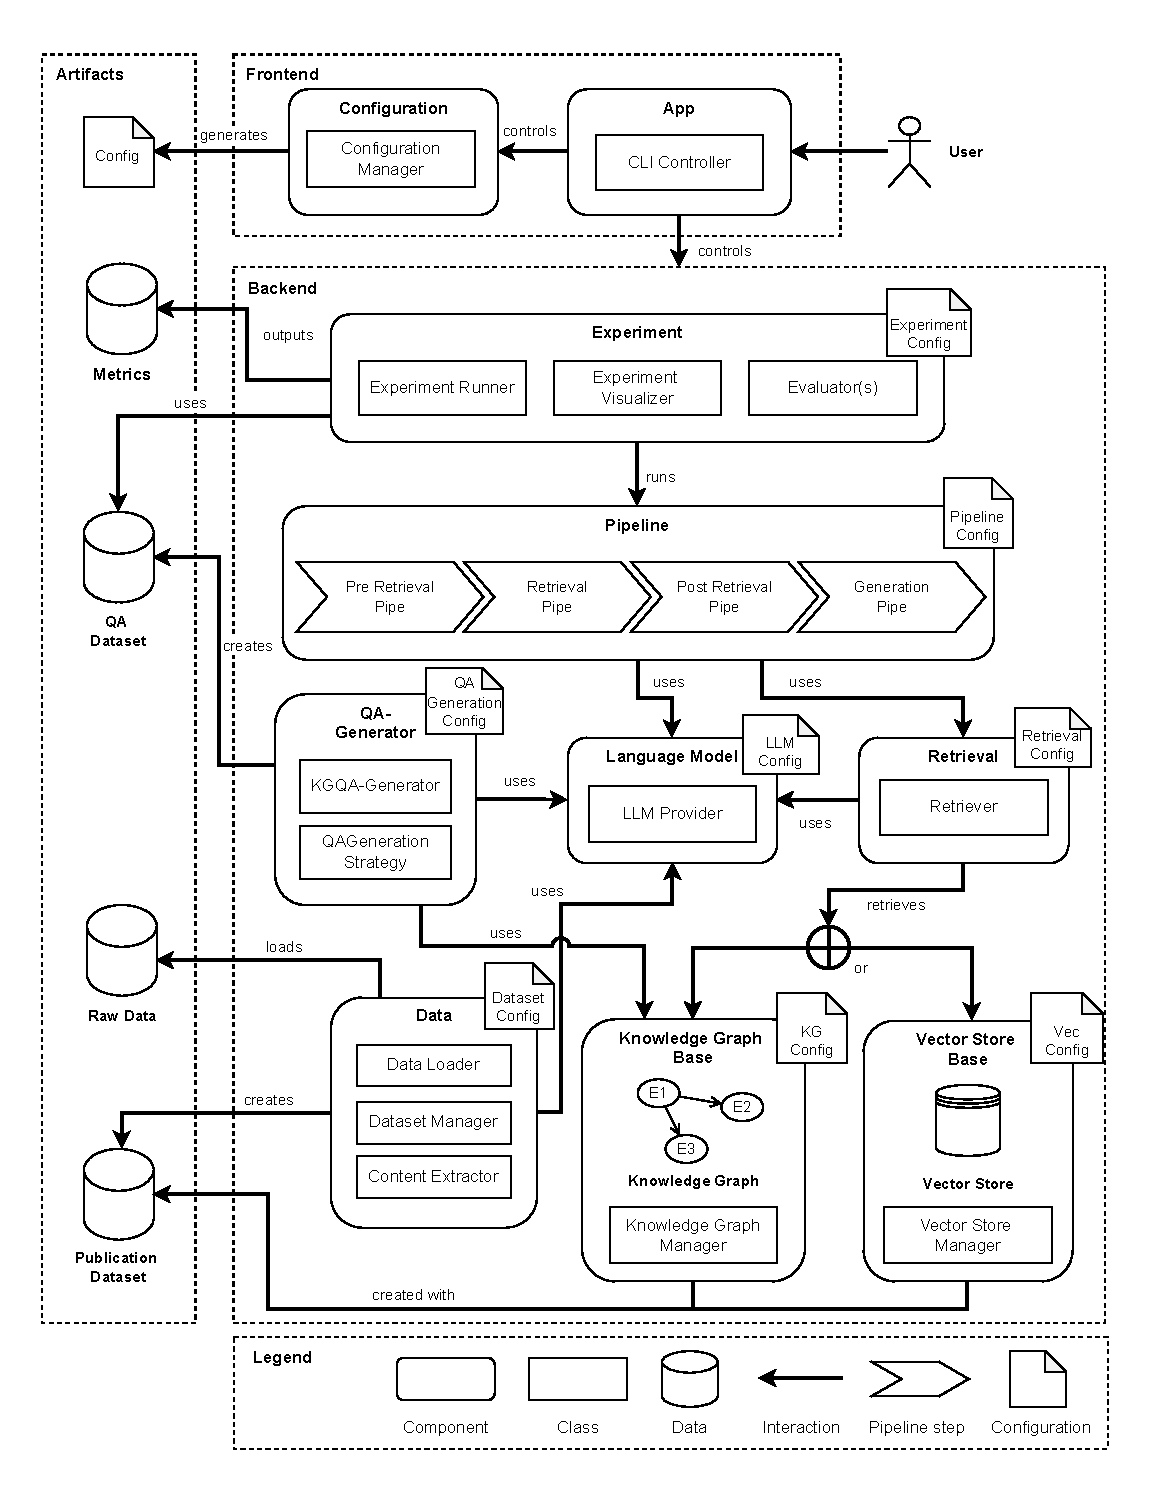
\includegraphics[width=0.99\linewidth]{figures/framework/overview-Architecture.drawio.pdf}
    \caption[SQA System Architecture]{Scholarly question-answering system architecture, illustrating key components and their primary interactions}
    \label{fig:overview_architecture}
\end{figure}

The \gls{sqa} framework is designed with extendability in mind. Consequently, it provides well-defined abstract interfaces and base classes to facilitate the straightforward integration of new \gls{kgqa} approaches, new \glspl{kg} or vector databases, different \glspl{llm}, and custom intermediate pipeline stages, ensuring the framework can adapt to future research directions and technological advancements. The framework employs a modular software architecture, as depicted in \autoref{fig:overview_architecture} to promote a clear separation of concerns, where each component encapsulates a specific set of functionalities. In the following, we briefly introduce each component of the \gls{sqa} framework before explaining them in detail:

\paragraph{Configuration Component}
The initialization and experimental setup are fundamentally based on the \emph{Configuration} component, which parses and validates JSON-based configuration files that define parameters and selected modules for all other components.

\paragraph{Data Component}
Data loading, preprocessing and distribution are the responsibility of the data component. It manages metadata and content data from publications, as well as \gls{qa} pairs from JSON and CSV sources, and makes these accessible to other parts of the system.

\paragraph{Pipeline Component}
The core logic of the question-answering process resides within the \emph{Pipeline} component. This component orchestrates the sequence of pipeline operations (pre-retrieval processing, context retrieval, post-retrieval processing, and final answer generation). 

\paragraph{Retriever Component}
Integrated closely with the pipeline, the \emph{Retriever} component performs the task of searching the designated \gls{kb} (\gls{kg} or vector index) to find contextually relevant information passages or facts relevant to the input question.

\paragraph{Language Model Component}
A unified interface for interacting with local or API-based \glspl{llm} is provided by the language model component. It handles \gls{llm} access for other components of the system and parses the response.

\paragraph{Knowledge Base}
A \gls{kb} stores and provides access to the data in the system. In the system, two types of \glspl{kb} are supported, which are \glspl{kg} and vector indices. Both are unified in the knowledge base component.

\paragraph{Experiment Component}
The experiment component provides the functionality to perform systematic evaluations. It iterates over specified configurations, executes the \gls{qa} pipeline for each test question, collects results, computes relevant \gls{rag} metrics, and stores these findings for later analysis.

\paragraph{QA Generator Component}
This component helps to create evaluation datasets by implementing semi-automated methods to generate \gls{kgqa} pairs from a \gls{kg} using an \gls{llm}.

\paragraph{App Component}
User interaction is managed through the app component, which offers a CLI application. This tool allows users to manage configurations, execute experiments, ingest data, and perform interactive querying of pipelines.

\subsection{Data Component}
\label{sec:sqas_architecture_inputs_outputs}

The \gls{sqa} system processes several types of data and features the structured \gls{llm}-based extraction of text. This section details the primary inputs and outputs handled by the system and describes the process of extracting structured data from paper texts.

\subsubsection{Inputs}

\begin{figure}[t]
    \centering
    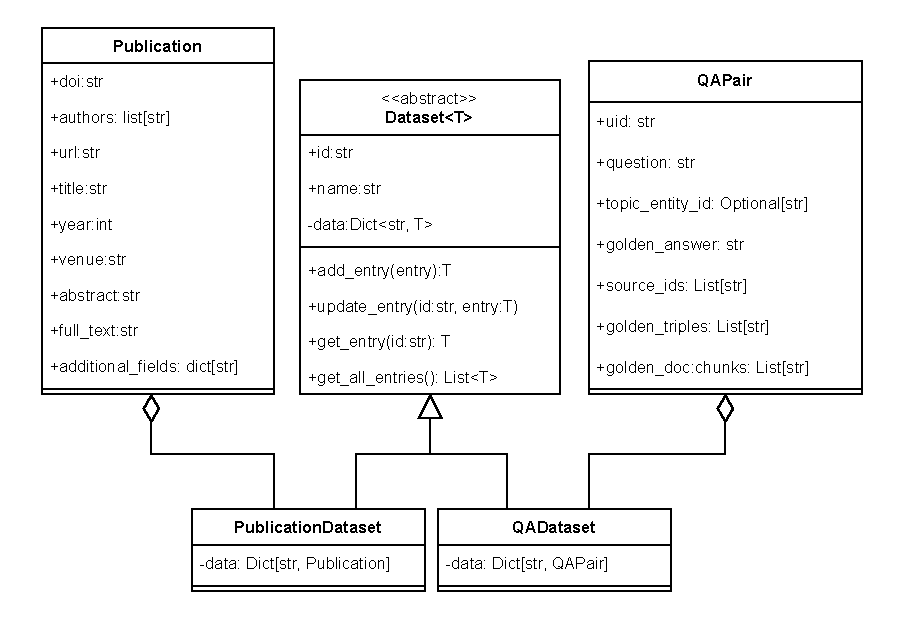
\includegraphics[width=0.99\linewidth]{figures/framework/figures-Input_data_models.drawio.pdf}
    \caption[Input Data Models of the SQA System]{Input data models of the \gls{sqa} system.}
    \label{fig:input_data_models}
\end{figure}

Any data that is inserted into the system has to be converted to either a \texttt{Publication} or \texttt{QAPair} object as depicted in \autoref{fig:input_data_models}. We introduce them in the following:

\paragraph{Publication Data:} 
An important data input of the \gls{sqa} framework is the metadata and content texts of scientific publications. These are ingested into the system from raw data, for example, in JSON format. For our experiments, we implemented a dedicated \texttt{JsonDataLoader}, which loads the publication data and converts it into the internal \texttt{Publication} data model that encapsulates both metadata and available full text for each scientific publication. To handle multiple publications, the \texttt{PublicationDataset} data model is used. This data model stores a collection of publications and provides easy access to them. The dataset is managed by the \texttt{DatasetManager} class, which enables other components to access datasets by providing configuration files. The manager then initiates the loading and handles the persistence.

\paragraph{Question-Answer Pair Data:} 
Question-answer pairs include the questions and ground truth to conduct the experiments. These are internally stored as \texttt{QAPair} objects in the \gls{sqa} system and loaded from data loader implementations from raw formats such as CSV. For our experiments, we implemented a \texttt{CSVDataLoader} that allows the serialized \gls{kgqa} dataset to be imported and used for the experiments. The \texttt{QAPair} data model has the following attributes:

\begin{enumerate}
    \item \textbf{UID:} A unique identification identifier that uniquely identifies the specific question-answer pair.
    \item \textbf{Question:} The natural language question posed to the \gls{qa} system.
    \item \textbf{Topic Entity:} An optional field specifying an entity within the target \gls{kg}, which potentially serves as an entry point for certain retrieval algorithms. It is optional as not all retrievers require this information.
    \item \textbf{Golden Answer:} A reference answer to the question, formulated in natural language, considered correct for evaluation purposes.
    \item \textbf{Golden Triples:} A set of triples present in the target \gls{kg} that represent the factual basis for the \emph{Golden Answer}.
    \item \textbf{Golden Text Chunks:} The text passages from source publications containing information that correspond to the \emph{Golden Answer} and align with the \emph{Golden Triples}.
    \item \textbf{Source IDs:} Identifiers of the source publications from which the \emph{Golden Answer}, \emph{Golden Triples}, and \emph{Golden Text Chunks} were derived.
\end{enumerate}

Similarly to the publication data, a collection of \texttt{QAPair} is handled by a \texttt{QADataset} data model. This model handles the access to the pairs and their persistence.


\subsubsection{Outputs}
Depending on the executed workflow (e.g., experimentation, interactive querying, \gls{qa} generation), the \gls{sqa} system produces several outputs:

\paragraph{Experiment Results:} 
When running an experiment, for each question several outputs are produced. These outputs include the generated answer and the retrieved context that both relate to the provided question. These outputs are then evaluated against the golden ground truth data provided by the \texttt{QADataset} using dedicated \texttt{Evaluator} objects. These produce comprehensive evaluation reports containing various \gls{rag} metrics (e.g., context relevance, answer faithfulness) and other measurements, which are then aggregated and exported in \texttt{CSV} format. Subsequently, an \texttt{ExperimentVisualizer} can be used to generate plots and tables to visualize the results.

\paragraph{Simple Answer:}
When executing a \gls{rag} pipeline in interactive mode, the primary output returned to the user is the generated natural language answer to the question posed.

\paragraph{QA Generation Data:} 
Another output comprises the semi-automatically generated \texttt{QAPair} objects, which are stored in a \texttt{QADataset} structure and serialized into \texttt{CSV} format for subsequent use in evaluations.

\subsubsection{Data Extraction}
The \gls{sqa} system also provides the ability to extract scientific content directly from the text of scientific publications. This process, orchestrated by the \texttt{ContentExtractor} class using a configured \gls{llm}, transforms unstructured text into structured data suitable for enriching \glspl{kg}. The extraction process involves the following steps:

\begin{enumerate}
    \item \textbf{Text Chunking:} The source text of the publication is segmented into smaller, manageable chunks suitable for processing by the context window limits of the \gls{llm}.
    \item \textbf{Chunk Extraction:} Each text chunk is processed by the \gls{llm}. To enhance completeness, this extraction is done multiple times for the same chunk. In subsequent extractions for the same chunk, previously extracted information is aggregated and provided back to the \gls{llm} as context to minimize redundancy.
    \item \textbf{Tracing:} Each extracted data item is mapped back to its location in the original publication source. This trace provides provenance for the information extracted.
\end{enumerate}

As mentioned above, the core extraction mechanism involves prompting the \gls{llm}. This is accomplished by populating a predefined \texttt{JSON} schema which defines the target information types, attributes, and relationships to be extracted (e.g., research methods used, research questions, key findings). The task of the \gls{llm} is to analyze the provided text chunk and accurately populate this schema with corresponding information found within the text. The data extracted from the schema can subsequently be utilized, for instance, in the construction of a \gls{kg}.

\subsection{Configuration Component}
\label{sec:sqas_architecture_configuration}

A primary goal during the development of the \gls{sqa} system was to ensure the easy definition and reproducibility of experiments. To achieve this, the system utilizes configuration files stored in \texttt{JSON} format. This storage method serializes configurations, enabling their persistence for future use and allowing experiments to be repeated accurately by using the corresponding files.

\begin{figure}
    \centering
    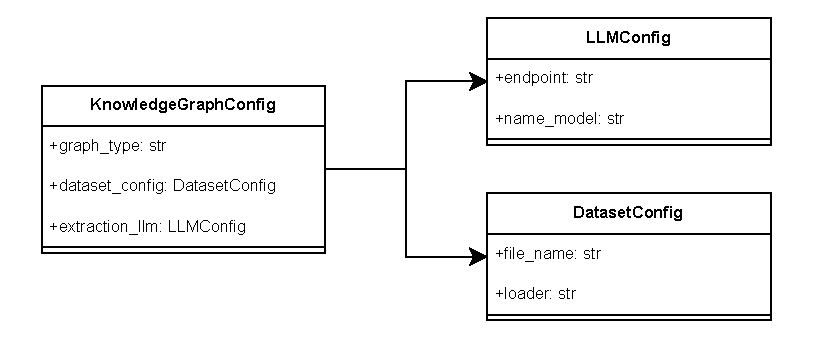
\includegraphics[width=0.90\linewidth]{figures/framework/figures-Bsp_Config_Model.drawio.pdf}
    \caption[Knowledge Graph Configuration Model]{The configuration model for a Knowledge Graph in the SQA system.}
    \label{fig:config_model}
\end{figure}

Each component of the \gls{sqa} system is controlled through a dedicated configuration file that defines its required parameters. An important characteristic of a configuration is that it can be hierarchically defined, meaning that one configuration may include another. \autoref{fig:config_model} shows the \gls{kg} configuration model as an example. It illustrates the parameters required, demonstrating that configurations can contain both primitive data types, such as strings and integers, and complex structures, like nested configuration objects.

To load the JSON files into the \gls{sqa} system the \texttt{ConfigurationManager} is responsible. This manager interprets the file to confirm that it is correctly structured and provides the filled configuration object to the relevant component that needs to be initialized. Furthermore, for reproducibility and caching, it is essential to determine whether two configurations are identical. This is achieved by calculating a cryptographic hash value for each configuration object. By calculating this hash over the content of the configuration, we ensure that the values of two configurations are only identical if and only if their contents are identical. This mechanism makes it easy to determine whether two configurations are the same. This functionality is used by components in the system to avoid duplicate instantiation in caching scenarios such as storing \gls{llm} models or \glspl{kg}. 



\subsection{Pipeline and Pipes Component}

The \gls{rag} process is implemented within the \gls{sqa} system using a pipeline architecture facilitated by the LangChain library\footnote{\url{https://www.langchain.com/} [last accessed on 12.05.2025]}. This pipeline accepts a question and, optionally, a topic entity as input. The pipeline processes this input and returns a \texttt{PipeIO} object populated with the results. The \texttt{PipeIO} object acts as a data container, progressively accumulating information such as the retrieved contexts and the generated answer as it traverses the pipeline stages. It also collects tracking data like carbon emissions or \gls{llm} token usage. 

In the following sections, we first describe the retrieval pipeline. Then, we detail the \texttt{PipeIO} data model.

\subsubsection{Retrieval Pipeline}
A standard pipeline comprises four distinct stages, referred to as \emph{pipes}. These pipes are executed sequentially in a predefined order: Execution starts with the \emph{Pre-Retrieval Pipe}, followed by the \emph{Retrieval Pipe}, then the \emph{Post-Retrieval Pipe}, and concludes with the \emph{Generation Pipe}. These pipes are explained in the following:


\paragraph{Pre-Retrieval Pipe:} 
This pipe is responsible for processing the input question before retrieval takes place. For example, the question given as input into the pipeline can be expanded to include synonyms or related terms to improve recall.

\paragraph{Retrieval Pipe:}
This is the pipe that is responsible for the extraction of relevant contexts from the underlying \gls{kb}. All retrievers are applied within this pipeline step. The task of the retriever is to identify and retrieve relevant context passages or structured data from the designated \gls{kb}. The retrieved contexts are then stored in the \texttt{PipeIO} object. In addition, certain retrievers may generate a final answer directly. If the retriever does not generate an answer, a subsequent \emph{Generation Pipe} is required to generate the answer.

\paragraph{Post-Retrieval Pipe:} 
This optional stage processes the contexts retrieved in the previous stage. Common operations include filtering irrelevant passages, reranking of contexts based on relevance or other criteria, or selecting a subset of contexts based on a specified criteria.

\paragraph{Generation Pipe:}
This pipe is responsible for synthesizing the final natural language answer. A configured \gls{llm} is invoked, provided with the original question and the retrieved contexts. The task of the \gls{llm} is to generate a coherent and factually grounded answer based on this input. The generated answer is then stored in the \texttt{PipeIO} object, completing the pipeline execution. This stage is optional if the retriever already produced a final answer.


\subsubsection{PipeIO Datamodel}
\begin{figure}[t]
    \centering
    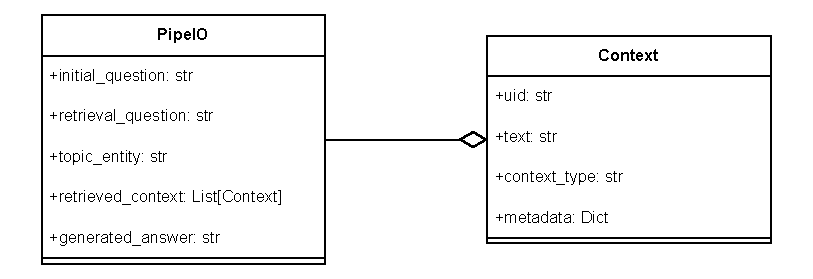
\includegraphics[width=0.90\linewidth]{figures/framework/figures-pipeIO_model.drawio.pdf}
    \caption[UML Diagram for the PipeIO Data Model in the SQA Framework]{The UML Diagram of the PipeIO model.}
    \label{fig:pipeio_model}
\end{figure}

The data model of the \texttt{PipeIO} object is shown in \autoref{fig:pipeio_model}. It contains several attributes that are populated by the individual pipes in the pipeline. Initially, the \texttt{PipeIO} data model is created by the pipeline, where the attributes \texttt{initial\_question}, \texttt{retrieval\_question}, and \texttt{topic\_entity} are initialized. The distinction between these two types of question exists because when the question is modified by the pre-retrieval pipe, the original question should still be saved. Consequently, the \texttt{initial\_question} attribute is \texttt{read-only}, while \texttt{retrieval\_question} can be modified. Furthermore, the topic entity can optionally be added. This allows retrievers to have an entry point in the \gls{kg} if they require it. Moreover, the \texttt{PipeIO} object contains the attributes \texttt{retrieved\_context} and \texttt{generated\_answer}. These attributes are filled during execution. 



\subsection{Retriever Component}
\label{sec:sqas_architecture_retriever}

\begin{figure}[t]
    \centering
    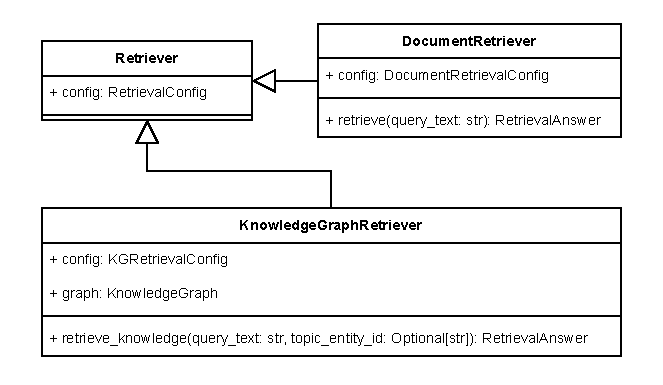
\includegraphics[width=0.80\linewidth]{figures/framework/figures-Retriever_UML.drawio.pdf}
    \caption[UML Diagram for Retrievers in the SQA Framework]{The UML diagram for retrievers in the SQA framework.}
    \label{fig:retriever_model}
\end{figure}

The main class in the retrieval component is the \texttt{Retriever}, which is responsible for finding relevant contexts from a \gls{kb} to answer a question. There are two sub-classes available for the \texttt{Retriever}: the \texttt{DocumentRetriever} and the \texttt{KnowledgeGraphRetriever}, each handling different types of data:

\paragraph{Document-based Retriever} works with text documents as input sources, specifically the full text of scientific publications. Unlike the \gls{kg} variant, the \texttt{DocumentRetriever} is not bound to a specific \gls{kb}. Instead, the corresponding \texttt{DocumentRetrievalConfig} specifies the configuration of the dataset, which contains the data that should be used for retrieval instead of a \gls{kg}.

\paragraph{Knowledge Graph-based Retriever} operates directly on a \gls{kg}. Instead of documents, it uses a \gls{kg} as the underlying data store. The configuration for the \gls{kg} is provided with the \texttt{KGRetrievalConfig} during the initialization of the retriever.

Once the retriever is implemented in the system, it is used in a pipeline to allow the retrieval of context for questions and to generate answers.

\subsection{Language Model Component}
\label{sec:sqas_architecture_language_model}

\begin{figure}[t]
    \centering
    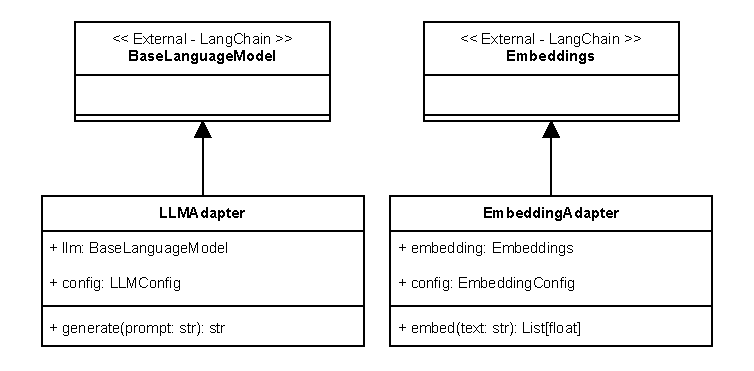
\includegraphics[width=0.80\linewidth]{figures/framework/figures-llm_model.drawio.pdf}
        \caption[UML Diagram for LLM and Embedding Adapters]{The UML diagram for the LLM adapter and Embedding adapter classes of the SQA system.}
        \label{fig:llm_model}
    \end{figure}

Since many components of the \gls{sqa} system work with \glspl{llm}, a dedicated \emph{Language Model} component is provided. This component offers a unified interface to make requests to an \gls{llm}. The requests, in conjunction with their corresponding configuration, are handled by the \texttt{LLMProvider}, which is responsible for initializing the model and establishing the connection.

The implementation of the models is achieved through the adaptation of the \texttt{BaseLanguageModel} and \texttt{Embeddings} classes from the LangChain\footnote{\url{https://python.langchain.com/docs/integrations/chat/} [last accessed on 28.01.2025]} library. The advantage of using the LangChain framework lies in its support for a wide range of models, a well-maintained interface, and easy integration of new models. Two types of adapters are implemented, which are shown in \autoref{fig:llm_model}. The \texttt{LLMAdapter} is responsible for sending requests to the \gls{llm} and processing the responses. The \texttt{EmbeddingAdapter}, on the other hand, handles the transformation of texts into vectors.

\subsection{Knowledge Bases Component}
\label{sec:sqas_architecture_knowledge_bases}

\begin{figure}[t]
    \centering
    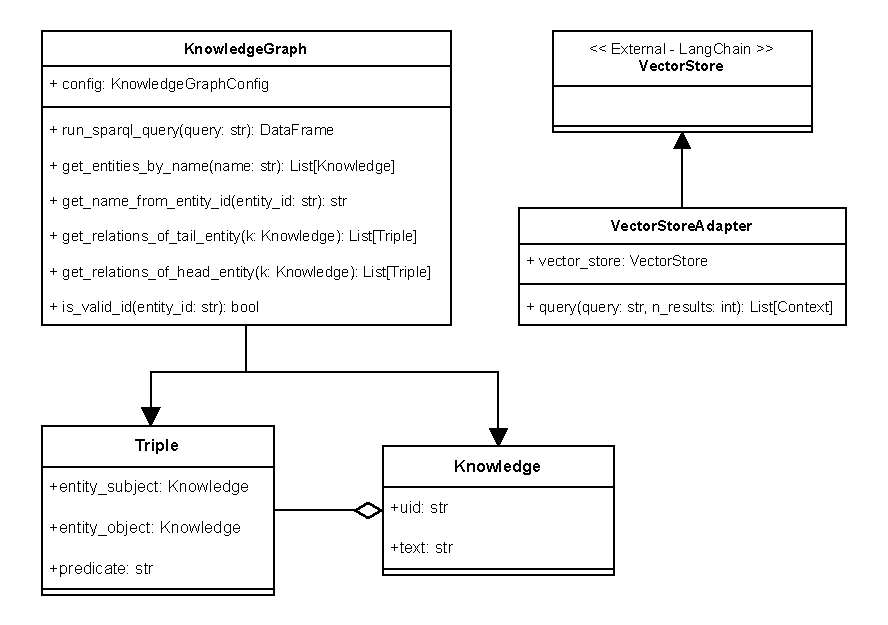
\includegraphics[width=0.99\linewidth]{figures/framework/figures-Knowledge_bases_uml.drawio.pdf}
    \caption[UML Diagram for KGs and Vector Stores]{The UML diagram for the knowledge graph and vector store.}
    \label{fig:knowledge_bases_model}
\end{figure}

The \gls{sqa} system provides two different types of \glspl{kb} as shown in \autoref{fig:knowledge_bases_model}: \glspl{kg} and vector stores. These \glspl{kb} can be used by retrievers to find relevant contexts for answering questions. In the following, we detail their implementations in the \gls{sqa} system:

\paragraph{Knowledge Graphs} are represented as \gls{rdf} graphs in the \gls{sqa} system. These graphs consist of triples represented with the \texttt{Triple} data model, which consists of \texttt{Knowledge} objects as shown in \autoref{fig:knowledge_bases_model}. Moreover, to manage and provide \texttt{KnowledgeGraph} objects in the \gls{sqa} system, the \texttt{KnowledgeGraphManager} is responsible. This manager initializes the graphs based on the provided configuration and caches their connection to allow other components to query the graph. The preparation or creation of a \gls{kg} is facilitated by the \texttt{KnowledgeGraphFactory}. This factory receives the graph configuration file and initializes or creates the \gls{kg} based on the given parameters.

\paragraph{Vector Stores} are specialized data structures that enable efficient vector storage and querying. They are used to store texts that have been transformed into a low-dimensional vector space using an embedding model. These vectors can then be used to calculate the similarities between texts. In the \gls{sqa} system, the \texttt{VectorStore} implementation from the LangChain library is adapted using a \texttt{VectorStoreAdapter}. Similarly to knowledge graphs, a \texttt{VectorStoreManager} is responsible for initializing, managing, and providing the vector stores.

\subsection{Experiment Component}

\begin{figure}[t]
    \centering
    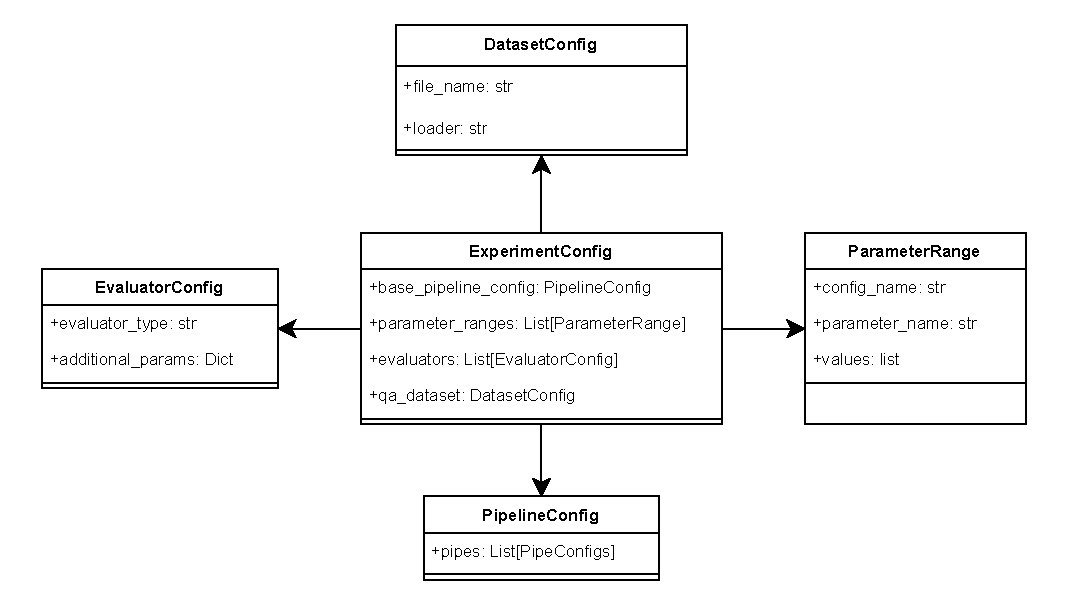
\includegraphics[width=0.99\linewidth]{figures/framework/figures-Experiment_model.drawio.pdf}
    \caption[UML Diagram for a Experiment Configuration]{The UML diagram for the experiment configuration}
    \label{fig:experiment_model}
\end{figure}

One of the main features of the \gls{sqa} system is the execution of experiments. These are defined using configuration files as described in Section~\ref{sec:sqas_architecture_configuration}. The UML diagram of an \texttt{ExperimentConfig} is shown in \autoref{fig:experiment_model}. This configuration contains all parameters necessary for conducting an experiment:

\begin{itemize}
    \item \textbf{Base Pipeline Config} is the configuration of the pipeline used for answering questions. It contains all the necessary parameters to initialize an \gls{rag} pipeline.
    \item \textbf{Parameter Ranges} are a list of parameters that allow varying the pipeline parameters within an experiment, which is useful for studying the effects of parameters on the results. The parameter configurations specified here are used by the \texttt{ExperimentRunner} to create multiple pipelines based on the base pipeline configuration, which are then executed in batch.
    \item \textbf{Evaluators} is a list of configurations for evaluators. These are classes in the \gls{sqa} system responsible for creating \gls{rag} metrics for the experiment.
    \item \textbf{QA Dataset} is the configuration of the \texttt{QADataset} used for the experiment. This contains the questions to be answered in the experiment, along with the corresponding ground truth data for evaluation.
\end{itemize}

The \texttt{ExperimentRunner} class is responsible for executing the experiment based on a configuration. This class takes the configuration and prepares the pipelines, which are then executed sequentially to fill the \texttt{PipeIO} object with data. Subsequently, the results of the pipeline are evaluated using the evaluators, which are also prepared by the runner. After the experiment has been conducted, the \texttt{ExperimentVisualizer} class is responsible for visualizing the results in diagrams and tables.

\subsection{Question Answering Generator Component}
\label{sec:qa_generator}
This component is responsible for the semi-automated creation of \gls{kgqa} pairs, which are stored internally as \texttt{QAPair} data models. The \gls{sqa} framework implements two different strategies for generating these \texttt{QAPair} objects: the \emph{Clustering Strategy} and the \emph{Subgraph Strategy}.

In the following, we first describe the clustering and subgraph strategy. Then, we explain the context and answer validation of the generated questions and answers.

\subsubsection{Clustering Strategy}
A significant challenge in generating \gls{kgqa} datasets is ensuring the completeness of the ground truth, particularly when an answer corresponds to multiple triples in the graph \cite{steinmetz_what_2021}. Ideally, the ground truth associated with a question should encompass all valid, relevant triples from the \gls{kg}. Incomplete ground truth can lead to misleading evaluations where systems are penalized for retrieving valid facts not included in the reference set. The \emph{Clustering Strategy} aims to address this challenge by identifying and grouping all potentially relevant facts before generating the question. The strategy operates as follows:

\begin{enumerate}
    \item \textbf{Provide Parameters:} The strategy is initialized with various parameters. One essential parameter is the topic entity from the graph. This entity serves as the starting point for the triple collection and is stored as the topic entity in the resulting \texttt{QAPair} object.
    
    \item \textbf{Build Publication Subgraphs:} The first step is to collect the subgraph for each publication containing triples that conform to user-provided restrictions. This requires the \emph{predicate type restriction} parameter, specifying the predicate identifier used to initially select relevant subgraphs. For each matching triple containing this predicate, the graph is traversed backward to locate the unique \enquote{paper type} triple that acts as the root node for the subgraph of the publication. Once the root is found, the strategy builds the subgraph by traversing outgoing edges until leaf nodes are reached. The result is a collection of publication subgraphs, each guaranteed to contain the specified predicate type.
    
    \item \textbf{Extract Values:} In the second step, the strategy extracts values of interest from each publication subgraph found previously, using a \emph{predicate value restriction} parameter defining the target predicate names. The strategy searches each subgraph for triples with matching predicates. Starting from these matching triples, it traverses all outgoing paths to leaf nodes, extracting their values. This produces a mapping from each extracted value of interest back to its source publication subgraph.
    
    \item \textbf{Cluster Values:} These extracted values of interest are then embedded into a vector space using a selected embedding model and subsequently clustered using the DBSCAN \cite{ester_density-based_1996} algorithm. This step forms clusters grouping semantically similar values. The mapping back to the source publication for each value is maintained throughout this process.
    
    \item \textbf{Additional Restrictions:} Based on these semantically coherent clusters, additional restrictions, which are also provided as parameters, can be applied. Each cluster is processed, and relevant triples conforming to these new restrictions are extracted from the associated publication subgraphs and added to the data payload of the cluster. The result is a set of clusters, each representing a semantic group of values and enriched with additional context triples.
    
    \item \textbf{LLM-based Generation:} After the clustering is done, the next step is the generation of the question and answer. Here, a \emph{template text} and \emph{additional instructions} for the \gls{llm} are provided as parameters to the strategy. The template is a question with placeholders to guide the \gls{llm} in the generation process, and the additional instructions are appended to the base prompt to further fine-tune the generation process. To generate the question and answer, the clusters are processed one by one and forwarded to the \gls{llm} with the prepared prompt. The \gls{llm} then generates a question and a corresponding answer given the data from the cluster, the template and instructions.
    
    \item \textbf{Prepare Ground Truth:} The triples accumulated within each cluster during the preceding steps serve as the ground truth. These are stored alongside the generated question and answer in the \texttt{QAPair} object.
    
    \item \textbf{Manual Validation:} Due to the potential for \gls{llm} hallucination or failure to adhere to instructions or templates, a final manual validation step is essential. The generated question and answer are checked for correctness, coherence, and adherence to the template. Consequently, the relevance and correctness of the collected ground truth triples must be manually verified.
    
\end{enumerate}

In the following, we illustrate an example to clarify the functionality of the clustering strategy. For this purpose, we use the following question template: \enquote{Which publications investigate the research object [research object name] and evaluate the sub-property [sub-property name]?}.

First, we need to ensure that all subgraphs containing the required information are fetched for further processing. In the case of the \gls{orkg}, we can directly use the unique identifier of the \emph{Research Object} predicate: $P162024$. This ensures that all publications that contain research objects are considered by the strategy.

Next, we define the list of predicate names that should be clustered from the subgraphs. Based on the question, we must specify the corresponding predicate names under which the requested information is stored in the graph. In our case, the predicates are labeled as \texttt{Research Object} and \texttt{Sub-Property}. In addition, further parameters can be defined to influence how the information is added to the clusters. For example, we can decide to split the clusters. In this case, the retrieved values are not added to the current cluster. Instead, a separate copy of the cluster is created for each value. This is desired for our question, as we do not want to collect all possible values of research objects and sub-properties in a single cluster but rather focus on specific instances.

At this step, each cluster contains all the publications of the dataset that investigate the same research object and evaluate the same sub-property. These clusters are now individually forwarded to the \gls{llm} that generates the question and the answer based on the triples in the cluster.

% This strategy allows for the creation of complex question-answer pairs. A major advantage over approaches solely reliant on SPARQL templates is the ability to group related information based on semantic similarity via clustering, rather than relying solely on explicit graph patterns. Furthermore, users provide predicate identifiers or names rather than formulating potentially complex SPARQL queries. Consequently, the strategy allows to automate the extraction and preparation of relevant graph data for generation.

\subsubsection{Subgraph Strategy} 
The second available strategy is the \emph{Subgraph Strategy}, which generates diverse question-answer pairs related to a single publication at a time. Unlike the cluster-based approach, this strategy does not inherently generate questions spanning multiple publications. Furthermore, it is less restrictive, which can enable the generation of a wider variety of question types. The strategy operates as follows:


\begin{enumerate}
    \item \textbf{Input Definition:} The strategy requires a publication entity from the \gls{kg} as input, which acts as a \emph{topic entity} identifier.

    \item \textbf{Subgraph Extraction:} Starting from the publication entity, the graph is traversed to extract the subgraph of the publication by traversing the graph until the leaf nodes are reached. However, this subgraph is limited to a predefined size to fit within the context window of the \gls{llm}.

    \item \textbf{LLM-based Generation:} This subgraph is then provided to the \gls{llm} with the instruction to generate both a relevant question and the corresponding golden answer. The generation process is guided by requiring the \gls{llm} to output a \texttt{JSON} structure containing the generated question, the answer and the specific subgraph triples that were used as the basis for generation.
\end{enumerate}


% \subsubsection{Techniques for Quality Assurance}
% To ensure the quality of the created \gls{qa} pairs, various techniques are employed, which are described below:

% \paragraph{Triple Tracing:} The \gls{sqa} system allows to extract structural data from the texts of publications. During this extraction, a tracing is generated and stored to map each generated triple back to the original text. This allows transparency and helps solve a challenge. Since the \gls{sqa} system also supports retrievers that work with documents (see Section~\ref{sec:sqas_architecture_retriever}), it is important to provide not only the golden triples but also the golden text passages. These are needed during evaluation to compare retrieved text passages with golden text passages and calculate metrics. Through tracing, the text passage, from which each triple in the golden triples was created, can be fetched and stored as a golden text passage in the generated \texttt{QAPair} object.

% When populating the \gls{kg} with data, we store the original text passage from which each triple was created, when this information is available. We can then use this mapping during \gls{qa} pair generation to improve the quality of the created questions and answers. This is utilized after the generator strategy selects the triples to be used for generating the question and answer. Instead of directly passing the triples to the \gls{llm}, we provide the text passage from which the triple was created by tracing the triple back to its original text passage. Using the original text passage allows to preserve more semantic context and thus improves the quality of the generated questions and answers. 

\subsubsection{Context and Answer Validation} 

During the generation of \texttt{QAPairs}, the \gls{llm} specifies golden triples that were used for the generation. We observed that this is not always accurate. Either the \gls{llm} indicates triples that do not match the generated answer, or the generated answer does not match the triples, indicating that the \gls{llm} is hallucinating. Therefore, we ensure through an additional validation process that the generated questions can actually be answered based on the data in the \gls{kg} and that the created answer truly matches both the question and the data. The validation process works as follows:

\begin{enumerate}
    \item \textbf{Triple Validation:} It may occur that initially, a larger set of triples was classified as relevant, but only a subset is actually necessary for answering the question. In this case, an \gls{llm} is prompted with a specially prepared validation prompt, and the triples as input. The \gls{llm} is instructed to ensure that all the information contained in the golden answer is present in the set of specified triples and to remove any triples that are not. This reduces the total set to the actually relevant triples or removes the question if no triples are relevant.
    
    \item \textbf{Answer Validation:} Furthermore, another \gls{llm} call is made to verify whether the generated answer matches the question.
    
    \item \textbf{Grammar Correction:} Since we observed that the generated questions are not always grammatically correct, an additional \gls{llm} call is performed to correct the generated question.
    
    \item \textbf{Manual Validation:} Finally, the generated data is manually reviewed before being saved to the final \texttt{QADataset}.
\end{enumerate}

\subsection{App Component}

The \emph{App} component includes a \gls{cli} application that enables users to operate the \gls{sqa} system through the command line. It offers the following functionalities:

\begin{enumerate}
    \item \textbf{Configuration Management:} All configurations of components in the \gls{sqa} system can be generated using the command line. This ensures that the configurations are well-defined.
    \item \textbf{Experiment Execution:} Experiments can be executed.
    \item \textbf{Question Answering:} Run pipelines in interactive mode for question answering.
\end{enumerate}

First, the \gls{cli} application enables configuration management. Since each configuration requires a different structure of the JSON file, it can be difficult for users unfamiliar with the system to create these files manually. Therefore, the \gls{cli} application provides guided configuration creation. This allows users to create configurations step by step and select the necessary parameters.

Furthermore, the \gls{cli} application facilitates direct execution of experiments based on created configurations. Users can select from a list of experiment configurations or create them directly. After executing the experiment, users receive a summary of results in the console, while detailed information is stored in a designated folder. This includes a CSV file containing all evaluations and experiment results. The results are also visually presented in diagrams that are saved in the folder. In addition, the configuration files are stored in JSON format in the folder to track which specific configuration led to the results.

Another feature of the \gls{cli} application is the interactive execution of pipelines. Users can select a pipeline configuration and ask a question. The pipeline is then executed for the question, and the answer is displayed in the console.

\section{Implementation of HubLink}
\label{sec:implementation_hublink}

We implemented our proposed HubLink approach by closely following the pseudocode outlined in \autoref{ch:hublink}. For the implementation, we used object-oriented programming, distributing specific responsibilities across different classes. Moreover, to accelerate index building and partial answer generation, we implemented parallel execution using multiple threads.

For the vector store, we chose Chroma\footnote{\url{https://www.trychroma.com/} [last accessed on 25.04.2025]} because it can run locally without a server, making it easy to use and only requiring the installation of a Python package. HubLink is seamlessly integrated into the \gls{sqa} framework and can be run using the configuration system provided. We implemented both proposed HubLink strategies to evaluate their performance on our \gls{kgqa} dataset.

\section[Accessing and Populating the ORKG]{Accessing and Populating the Open Research Knowledge Graph}
\label{sec:implementation_orkg}

Our experiments are conducted on the \gls{orkg} as the underlying \gls{rkg}. This section details the implementation and the setup of the \gls{orkg} for these experiments. We first outline the \gls{orkg} environment and the \gls{api} used for the connection. Subsequently, we introduce the dataset of scientific publications employed in our study. We then describe the contribution templates designed to structure this data within the \gls{orkg} and the procedure for populating the graph accordingly. Finally, we address the measures implemented to ensure experimental repeatability and detail the methodology for selectively reading data from the graph that are relevant to specific experimental configurations from the \gls{orkg}.


\subsection{ORKG Environment and API}
\label{sec:orkg_environment_and_api}

The \gls{orkg} is hosted on three different environments. The \emph{production}\footnote{\url{https://orkg.org/}} environment provides access to the current version of the graph and is the most stable version. The \emph{sandbox}\footnote{\url{https://sandbox.orkg.org/}} is a playground environment that is intended for experimentation on the \gls{orkg}. Finally, the \emph{incubating}\footnote{\url{https://incubating.orkg.org/}} environment is used to test new features that are still under development. We will conduct our experiments in the \emph{sandbox} environment.

To access this environment, the backend is exposed over a RESTful \gls{api} that is accessible online\footnote{\url{https://tibhannover.gitlab.io/orkg/orkg-backend/api-doc/}[last accessed on 09.04.2025]} and a Python package\footnote{\url{https://orkg.readthedocs.io/en/latest/index.html}[last accessed on 09.04.2025]}. The RESTful \gls{api} provides all read and write operations that are publicly available, and the Python package acts as a wrapper to provide easy access directly through code. However, at the time of writing, the package is still in development and does not yet provide the full list of features provided by the RESTful \gls{api}. Consequently, we are using the Python package to store information in the graph, and we use the RESTful \gls{api} for reading operations.

\subsection{Dataset of Scientific Papers}
\label{sec:experiments_dataset}

\begin{table}[t]
    \centering
    \begin{tabularx}{\textwidth}{l X l}   
        \toprule
        \textbf{Data Item} & \textbf{Description} & \textbf{Type}\\
        \midrule
            Paper Class & A general classification of the publication. & Meta Data \\
        \cmidrule(l){1-3}
            Research Level & Distinguishes on whether the research is collected firsthand. & Meta Data \\
        \cmidrule(l){1-3}
            Kind & Classifies whether the paper can be seen as a full research paper. & Meta Data \\
        \cmidrule(l){1-3}
            Research Object & The investigated object(s) of research. & Content Data \\
        \cmidrule(l){1-3}
            Tool Support & Indicates whether the paper employed a tool. & Content Data \\
        \cmidrule(l){1-3}
            Input Data & Indicates whether the paper used specific input data. & Content Data \\
        \cmidrule(l){1-3}
            Replication Package & Indicates whether the paper provides a dedicated replication package. & Content Data \\
        \cmidrule(l){1-3}
            Threats to Validity (TtV) & The threads to validity that are named in the paper. & Content Data \\
        \cmidrule(l){1-3}
            TtV Guideline & Indicates whether the paper references TtV guidelines. & Content Data \\
        \cmidrule(l){1-3}
            Evaluation Method (EM) & The applied evaluation method. & Content Data \\
        \cmidrule(l){1-3}
            EM Guidelines & Indicates whether the paper referenced guidelines for EM. & Content Data \\
        \cmidrule(l){1-3}
            Property & The property that is evaluated with a EM for a research object. & Content Data \\
        \bottomrule
    \end{tabularx}
    \caption[Data Schema for SWA Publications]{Extraction data schema applied in the work of \textcite{konersmann_evaluation_2022}}
    \label{tab:swa_data_schema}
\end{table}

To evaluate how well HubLink performs in the context of scholarly literature searches, we require a dataset of scientific publications. For this purpose, we use the dataset provided by \textcite{konersmann_evaluation_2022}. This dataset was originally created to analyze how \gls{swa} research objects are evaluated and how replication packages are provided. It was created through a literature search and annotations were extracted according to a specific schema. In their study, a total of 153 publications were included according to the following inclusion and exclusion criteria:

\begin{enumerate}
    \item Papers presented at \gls{ecsa} and \gls{icsa} conferences between 2017 and 2021.
    \item Comprehensive technical papers, excluding short papers, experience reports, and opinion pieces.
    \item Papers focusing on evaluation research, validation studies, solution proposals, and philosophical discussions.
\end{enumerate}

The schema employed for this annotation process is presented in \autoref{tab:swa_data_schema}. Each publication is annotated according to its research objects, research level, paper class, and validity information. The table also categorizes data as either metadata or content data. The differentiation between metadata and content data presented in \autoref{tab:swa_data_schema} is based on the information provided by \textcite{konersmann_evaluation_2022}.

According to \textcite{riley_understanding_2017}, metadata is defined as \enquote{data that provides information about other data}. In the context of the data schema defined in \autoref{tab:swa_data_schema}, two types of metadata are present: \emph{descriptive} and \emph{preservation}. Descriptive metadata provides information for finding or understanding a resource, such as the title, authors, and publication year. Preservation metadata, a subtype of administrative metadata, encompasses information regarding the long-term management of a file \cite{riley_understanding_2017}.

In addition to metadata, the dataset also contains content data, which we define as information \emph{that is contained within} the scientific artifact. This implies that to obtain the desired content data, the text of the publication must be read.

The extracted annotations in the dataset are based on the content of the publications and have been scientifically validated. Combined with the corresponding metadata, this dataset is well suited for our experiments, as it allows us to formulate questions regarding both metadata and content. We therefore compiled the data and consolidated them into a single JSON file to be used during our experiments. The resulting dataset consists of 153 publications, with the annotations shown in \autoref{tab:swa_data_schema}. In addition to the annotations, the dataset also includes metadata such as title, authors, \gls{doi}, and publication year.

\subsection{Contribution Templates}
\label{sec:contribution_templates}

To add new scholarly contributions to the \gls{orkg}, the graph allows users to include publications by providing a \gls{doi} or the title. The publication is then either linked to an existing resource in the graph or a new resource is created. In both cases, the system automatically fills in the metadata. After this step, the graph contains only the metadata of the paper. To specify what scientific contributions the paper makes, this information is added using the \emph{Contribution} \gls{orkg} content type. In other words, all the knowledge presented in a paper is added to the graph through one or more contributions \cite[58-60]{ilangovan_open_2024}.

For the purpose of our experiments described in Section~\ref{sec:experiments_dataset}, we needed to load the labels provided by \cite{konersmann_evaluation_2022} into the \gls{orkg}. To do so, we created templates for individual contributions to attach to each publication. We decided to design four different graph variants in order to test the robustness of the HubLink retriever against these variations. These variants are shown in \autoref{fig:overview_graph_variants}. The idea behind splitting the content into different variants is to maintain the same informational content while varying the depth and breadth at which it is stored. Depth refers to how far the information is stored from the root node of the paper, whereas breadth refers to whether the information is semantically separated across multiple contributions or centrally stored within a single contribution. The following four variants have been prepared:

\begin{figure}
    \centering
    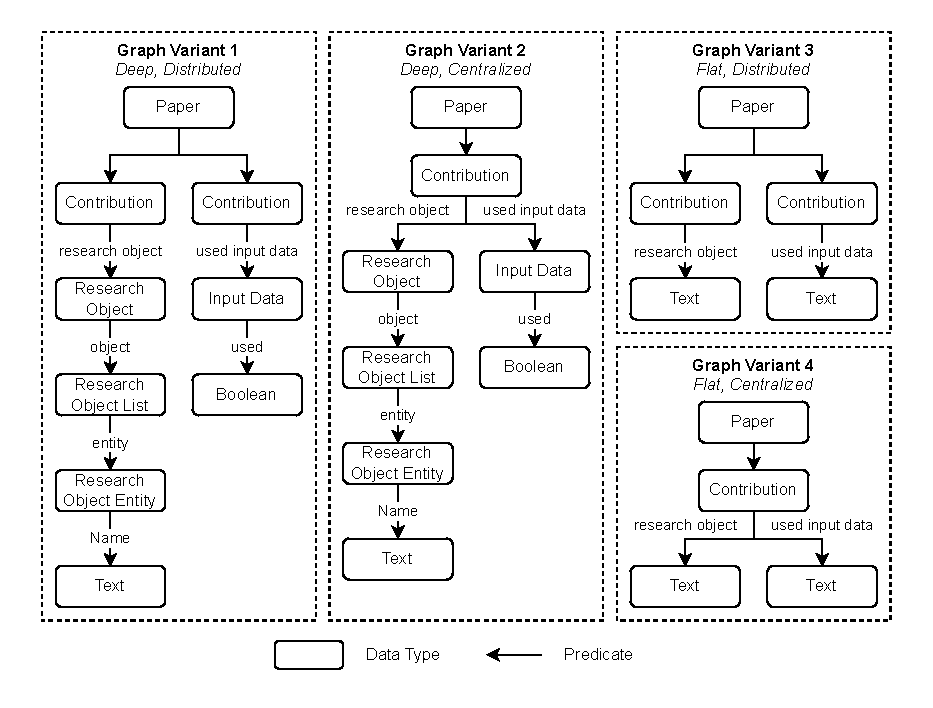
\includegraphics[width=0.93\linewidth]{figures/orkg/template_overview-graph_variants.drawio.pdf}
    \caption[Overview of our Experimentation Graph Templates]{Excerpt of the four different graph variants of the \gls{orkg} featuring the fields research object and input data. This figure highlights the difference between the depth and width of how the same information is stored in each of the different graph variants.}
    \label{fig:overview_graph_variants}
\end{figure}

\begin{enumerate}[leftmargin=2.5em] 
    \item[\textbf{GV1}]\label{enum:gv1} This graph variant stores data in long paths. In addition, the information is semantically separated and distributed between different contributions. 
    \item[\textbf{GV2}]\label{enum:gv2} This graph variant stores data in long paths. All information is collected in a single contribution. 
    \item[\textbf{GV3}]\label{enum:gv3} This graph variant stores data in short paths. The information is semantically separated and distributed across different contributions. 
    \item[\textbf{GV4}]\label{enum:gv4} This graph variant stores data in short paths. All information is collected within a single contribution. 
\end{enumerate}

An illustrative example depicting an excerpt from each of the variants is presented in \autoref{fig:overview_graph_variants}, while the full templates are provided in Appendix~\ref{sec:appendix:orkg_contribution_templates}. The figure shows the root entity of a paper and how information about input data and research objects is stored for each of the four different variants. This highlights the difference in depth and breadth in which the same information is stored between templates.

Using these variants, our aim is to test how robust HubLink is with respect to different graph structures. Long paths allow more information to be stored, but also require more processing. In contrast, short paths limit the amount of stored information, which may result in the loss of semantic context. In addition, we want to examine whether the distribution of data between one or multiple contributions has an effect on performance. Moreover, templates differ in the types that they use to store the data. Consequently, if a \gls{kgqa} approach can be applied to any of the graph variants without requiring a change in its configuration or implementation, it indicates that the approach is \emph{schema-agnostic}. 

The most difficult design decision during the creation of the templates was the multiple classification types in our data. These involve the classification of a paper according to a specific term from a specific selection of terms. For example, whether the paper class is evaluation research, a proposal for a solution, or validation research. To store such information, a typical user interface would provide a \emph{multiple-choice} data type. However, the template system provided by \gls{orkg} does not provide such a datatype at the time of writing. We therefore needed to create such a multiple-choice concept ourselves with the structures provided by the \gls{orkg}. This encompasses several considerations that must be taken into account.

We considered two choices to realize multiple choice. Using \emph{plain text} would allow users to flexibly input their choices. Nevertheless, this approach would not enable the template author to constrain the input, which would be against the idea of consistency in the data, because contribution data types that may relate to the same concept are not guaranteed to have the same value. This includes simple issues like casing, typos, synonyms, etc. Another realization would be a \emph{List of Boolean values}. This would allow the template author to create a list with predefined choices that are relevant. Each choice would be of the type Boolean to determine whether the choice is selected or not. However, the drawback of this approach is that it is less flexible for future extensibility. If the list is later updated to include more choices, all papers that have already used the template will have an empty value for the new choice. However, solving this issue is beyond the scope of this thesis. We implemented both methods in our templates. The variants \textbf{GV1} and \textbf{GV2} implement the list of Boolean, while the variants \textbf{GV3} and \textbf{GV4} store each choice in plain text. The concrete templates for each variant are provided in the Appendix \ref{sec:appendix:orkg_contribution_templates}.

\subsection{Populating the ORKG with Data}
\label{sec:populating_the_orkg}

To store data in the ORKG graph using various templates, a dedicated script was implemented. This script reads the metadata and annotations of the publications from a JSON file and processes each entry iteratively. For each publication, it checks whether it already exists in the graph with all specified contributions. If not, the corresponding contribution is added and populated with the relevant data. The script is triggered automatically whenever the \gls{sqa} system initializes the \gls{orkg} class, which happens before each experiment is run. 

\subsection{Ensuring Repeatability}
\label{sec:orkg_ensuring_repeatability}

During the implementation of the \gls{orkg}, it became evident that inserting data into the graph leads to the automatic generation of unique resource IDs. These IDs cannot be manually controlled and will change if data is deleted and then reinserted into the graph. This poses a challenge since the \gls{kgqa} dataset stores these resource IDs as part of the ground truth to verify whether the correct triples are retrieved during evaluation. If the original data are removed and later reinserted, new resource IDs are generated, which invalidate the \gls{kgqa} datasets.

To address this issue, a script was developed that compares the resource IDs stored in the \gls{kgqa} dataset with the IDs in the graph and updates the IDs in the dataset accordingly. With this approach, we can ensure that the experiments remain reproducible over time. Specifically, this means that the publications can be automatically reinserted into the \gls{orkg} using the \gls{sqa} system in the case that they have been deleted. The system then runs a script that updates the corresponding IDs in the \gls{kgqa} dataset.


\subsection{Reading from the ORKG}
\label{sec:reading_from_the_orkg}

To retrieve data stored in the \gls{orkg}, we use the provided RESTful \gls{api}. This API was integrated into the \gls{sqa} system to enable the automated execution of the experiments. However, during implementation, a key challenge emerged. The \gls{orkg} contains a large amount of data not relevant to our experiments. These additional data introduce noise, making it difficult to establish a controlled experimental setting. Another issue we encountered is that standard users have limited ability to delete data in the \gls{orkg}. This became an issue with our four different graph variants, as the individual deletion of contributions was not possible. Consequently, we stored all variants simultaneously in the graph.

To ensure that an experiment operates only on the data relevant to the experiment, a tailored solution was implemented. During the initialization of the \gls{orkg}, a preprocessing step generates a locally stored list of valid entities and triples. This involves examining all entities and triples in the research field \emph{Software Architecture and Design}, which contains the data relevant to our experiments. Each entity and triple is checked to determine whether they are part of the metadata of a relevant publication or belong to a contribution associated with the currently selected graph variant. Only those triples and entities that meet these criteria are included in the list.

At runtime, this list acts as a filtering mechanism: for each read request made by a retriever, only those triples and entities contained in the prepared list are returned. This ensures that only the intended data for the specific experiment, and exclusively from the selected graph variant, are taken into account.


\section{Baseline KGQA Retrieval Approaches}
\label{sec:implementation_baselines}

To evaluate our HubLink approach against existing \gls{kgqa} approaches, we implemented five distinct baseline methods within the \gls{sqa} system. This section details the selection process and the implementation of these baselines. First, we outline how candidate approaches were identified and filtered. Then, we explain the methodology of each selected retriever and briefly describe its implementation.

% The retrievers have been implemented using the provided interface of the \gls{sqa}. Consequently, the parameters with which the retrievers are initialized are controlled using a JSON configuration file that is injected before experiment initialization.

\subsection{Selection of Baselines Approaches}

To compare HubLink with state-of-the-art methods from the literature, we selected and implemented several approaches drawn from recent publications. The chosen baseline approaches represent established methods within the field previously evaluated on open-domain \gls{kgqa} benchmarks. In the following, we outline the systematic process through which these methods were chosen.

\subsubsection{Collecting Paper Candidates} 

Recently, surveys have been published that structure the current approaches found in the literature. \textcite{pan_unifying_2024} provide an in-depth analysis of the integration of \glspl{llm} with \glspl{kg}, which includes \gls{kgqa} but also goes beyond that. In their work, they propose a categorization of different integration strategies, assigning each examined paper to one of these categories. From this structure, we selected the categories relevant to \gls{kgqa}, namely \emph{KG-Enhanced LLM - Inference}, \emph{LLM-Augmented KG - Question Answering}, and \emph{Synergized Reasoning}, as these directly address the integration of \glspl{llm} and \glspl{kg} for question-answering tasks. 

Another survey by \textcite{peng_graph_2024} proposes a taxonomy for \gls{grag} approaches, which classifies the methods in a range of dimensions. From this set, we include all publications covered by the survey, except those classified as \emph{Non-parametric}, \emph{GNN-based} retrievers, or those considered \emph{Training-based}. 

In addition to the surveys, we conducted a Google Scholar search to identify further \gls{kgqa} approaches. Since both surveys were published in 2024, we limited our search to this year in order to find additional approaches not yet captured by the surveys.


\subsubsection{Excluding Papers not Relevant}

Through the above-mentioned surveys and Google Scholar search, we collected an initial pool of 76 publications. The next step was to identify the \gls{kgqa} approaches most relevant for comparison with HubLink by applying the following exclusion criteria to each of the publications:

\begin{enumerate}[label=\textbf{[C\arabic*]}]
    \item \textbf{LLM-Based:} The approach proposed in the publication must employ a pre-trained \gls{llm} to support the retrieval process. Embedding models are also included under this criterion. This is relevant because our objective is to explore how \glspl{llm} can support literature search within a \gls{qa} context.
    \item \textbf{KGQA Approach:} The approach proposed in the publication must represent a generalizable \gls{kgqa} approach. Specifically, it should accept a question in natural language and a \gls{kg} as input, with the goal of extracting relevant information from the \gls{kg} to answer the question.
    \item \textbf{Training-Free:} The approach proposed in the publication must not require additional training or fine-tuning of pre-trained \glspl{llm}, nor the training of other models such as \glspl{gnn}. Consequently, all approaches that depend on a dataset of training examples have been excluded, as we lack the resources for extensive training.
\end{enumerate}

Applying these criteria to the collection of 76 publications resulted in 13 relevant papers. Specifically, one paper was excluded for not using an \gls{llm} (\textbf{C1}), 21 were excluded as they did not represent a suitable \gls{kgqa} approach (\textbf{C2}), and 41 were excluded for requiring model training (\textbf{C3}). The complete list of candidates and the filtering results are provided in the replication package \cite{schneider_replication_2025}.

\subsubsection{Assessing Implementation Feasibility}

For the remaining 13 papers deemed relevant, we evaluated the availability and applicability of their implementations provided by the authors for integration into the \gls{sqa} system.

The approaches RoK \cite{wang_reasoning_2024} and KSL \cite{feng_knowledge_2023} were excluded as they do not provide source code. Their complexity made reimplementation impractical without access to the original code.

In the case of KG-GPT \cite{kim_kg-gpt_2023}, after reviewing the code repository\footnote{\url{https://github.com/jiho283/KG-GPT} [last accessed 24.11.2024]}, we found that the implementation corresponds to a claim verification pipeline rather than a traditional \gls{qa} setting. This assumes a prior mapping of claim entities to graph entities, which is not available in our use case.

For ODA \cite{sun_oda_2024}, although the authors provide a repository\footnote{\url{https://github.com/Akirato/LLM-KG-Reasoning} [last accessed 24.11.2024]}, it contains only graph and dataset resources, lacking the implementation of the ODA approach itself.

DiFaR \cite{baek_direct_2023} does not have a public implementation. However, its methodology closely resembles the \gls{rag} framework \cite{lewis_retrieval-augmented_2021}, differing mainly in embedding graph triples instead of documents. Given the experience of the thesis author with similar architectures, we deemed reimplementation feasible based on the description of the paper.

For the remaining methods: StructGPT \cite{jiang_structgpt_2023}, ToG \cite{sun_think--graph_2024}, Mindmap \cite{wen_mindmap_2024}, ToG-2 \cite{ma_think--graph_2024}, GoG \cite{xu_generate--graph_2024}, GRAPH-COT \cite{jin_graph_2024}, and FiDeLiS \cite{sui_fidelis_2024}, we found that the provided source code was generally adaptable for integration into the \gls{sqa} system.

\subsubsection{Deciding on Final Implementations}

After assessing implementation feasibility, eight of the 13 methods remained as candidates: StructGPT, ToG, Mindmap, ToG-2, GoG, GRAPH-COT, FiDeLiS, and DiFaR. To keep the scope of this work manageable, we ultimately selected five of these for implementation, guided by their methodological diversity. We categorize the eight candidates as follows:

\begin{itemize}
    \item \textbf{Stepwise reasoning:} These approaches iteratively query the \gls{llm} to derive an answer step by step. This category includes: StructGPT \cite{jiang_structgpt_2023}, ToG \cite{sun_think--graph_2024}, ToG-2 \cite{ma_think--graph_2024}, GoG \cite{xu_generate--graph_2024}, GRAPH-COT \cite{jin_graph_2024}, and FiDeLiS \cite{sui_fidelis_2024}.
    \item \textbf{Subgraph construction:} These methods focus on building relevant subgraphs from which information is extracted. Mindmap \cite{wen_mindmap_2024} is the only candidate in this category.
    \item \textbf{Embedding-based:} These methods primarily use dense vector representations for retrieval. DiFaR \cite{baek_direct_2023} is the only candidate here.
\end{itemize}

During the conceptual phase of this work, prior to this baseline selection, StructGPT \cite{jiang_structgpt_2023} and ToG \cite{sun_think--graph_2024} were implemented to evaluate the general feasibility of the thesis. At the time, both were highly cited and provided an adaptable public code. However, these approaches are very similar and share a weakness particularly relevant to scholarly literature search, as their entity selection can become random beyond a certain threshold, making correct entity identification dependent on chance. This significantly impacts the quality of the answer, as detailed in Section~\ref{sec:discussion_on_evaluation_results}.

Although ToG-2 \cite{ma_think--graph_2024}, a successor to ToG, was published during the conduct of this thesis, the issue described above was not resolved in the new version. For this reason, we decided not to implement this approach. Instead, we selected FiDeLiS \cite{sui_fidelis_2024} from the Stepwise reasoning category, as it specifically addresses the entity selection problem using an embedding-based similarity assessment. This brings the total number of implemented methods in the Stepwise reasoning category to three.

In the Subgraph construction and Embedding-based categories, only Mindmap \cite{wen_mindmap_2024} and DiFaR \cite{baek_direct_2023} remained after filtering. Therefore, both were implemented as baselines, bringing the total number of baseline methods implemented to five.




\subsection{Direct Fact Retrieval (DiFaR)}

\gls{difar} is a \gls{kgqa} retrieval approach proposed by \textcite{baek_direct_2023}. It was evaluated on fact retrieval tasks across two different domains: \gls{qa} and dialogue generation. For \gls{qa}, three different datasets were used: \textsc{SimpleQuestions} and \textsc{WebQuestionsSP} for the Freebase graph, and \textsc{Mintaka} for the Wikidata graph. For dialogue generation, they used the \textsc{OpenDialKG} dataset designed for the Freebase graph. Their tests show that the approach outperforms all baselines, although performance is lower for intrinsically more complex multi-hop retrieval questions.


\subsubsection{Approach Explanation} 
The retriever first undergoes an indexing phase, during which it converts all triples in the \gls{kg} into a set of embeddings. At query time, the question is embedded using the same embedding model that was used for the triple conversion. Subsequently, a nearest-neighbor search is performed to find the triples whose embeddings are closest to the question embedding, thus enabling a quick search through potentially billions of dense vectors. These triples serve as the context for answering the question. The researchers further propose a refinement, termed DiFaR2, involving a reranking of the retrieved triples. This approach utilizes a language model provided with both the question and the retrieved triples to evaluate triple relevance.

\subsubsection{Approach Implementation} 
We implemented the \gls{difar} approach based on the descriptions provided in the paper. In our implementation, the indexing process starts by selecting an initial entity within the graph and then traversing sequentially from it. Each triple collected during traversal is then embedded using a pre-trained embedding model. The specific embedding model is selected based on the provided configuration file. These vectors are then stored in a vector store. At query time, the question is processed to generate its embedding. This embedding is used in a \gls{ann} search on the data stored in the vector store. The triples retrieved from this search are then incorporated into an \gls{llm} prompt for the generation of the final answer. Regarding the proposed reranking, the \gls{sqa} system already provides a post-retrieval procedure that reranks contexts based on relevance, which can be enabled via configuration.




\subsection{Think-on-Graph (ToG)}

\textcite{sun_think--graph_2024} propose \gls{tog}, a \gls{kgqa} retrieval approach based on beam search. The authors evaluated their approach on nine different datasets for the Freebase and Wikidata graphs to demonstrate its advantage in reasoning over knowledge-intensive tasks. The datasets used for Freebase were \textsc{ComplexWebQuestions}, \textsc{WebQuestionsSP}, \textsc{GrailQA}, \textsc{SimpleQuestions}, and \textsc{WebQuestions}. For the Wikidata graph, the datasets were \textsc{QALD10-en}, \textsc{T-REx}, \textsc{Zero-Shot RE}, and \textsc{Creak}. Their tests show that \gls{tog} achieves state-of-the-art performance on six out of the nine datasets.

\subsubsection{Approach Explanation} 
The process is initialized with topic entities, which act as entry points into the graph. Starting from these entities, an exploration takes place. During exploration, the system iteratively traverses the \gls{kg} to build reasoning paths. At the start of each iteration, the current set of reasoning paths includes all entities and relations discovered so far. The \gls{llm} identifies candidate relations by querying the \gls{kg} for relations connected to the tail entities of the paths of the previous iteration. These relations are ranked by their relevance to the question. The top N are then selected using an \gls{llm}-based pruning step to narrow the search space. Next, the \gls{llm} uses the selected relations to find candidate entities, which are then randomly pruned to stay within a predefined threshold specified in the parameters. The reasoning paths are updated with the newly discovered entities and relations, effectively increasing their depth by one with each iteration.

The reasoning phase follows, involving evaluation and potential termination. The \gls{llm} evaluates whether the current reasoning paths contain enough information to answer the question. If so, it generates an answer using these paths. If not, exploration continues until either an answer can be formulated or a predefined maximum depth is reached. If sufficient information is not found by then, the \gls{llm} resorts to its internal knowledge to produce a response.


\subsubsection{Approach Implementation} 
The original code provided by the authors is available online\footnote{\url{https://github.com/IDEA-FinAI/ToG/} [last accessed 21.11.2024]}. We adapted their code with minimal necessary changes to work with the \gls{sqa} system interface. During testing, we encountered several issues requiring further adjustments. First, many executions failed because some outputs of the \gls{llm} deviated from the expected output format. We found that the original parser was unable to handle these variations in \gls{llm} output. To address this, we developed a more robust parser capable of extracting information from a wider range of \gls{llm} outputs. Second, we parallelized the entity searching and scoring processes, as the original sequential implementation was inefficient. Third, the original implementation only returned the \gls{llm}-generated answer. We extended the output to also return the triples used to generate the answer to allow for evaluation of retrieval performance. Finally, many of the prompts used by the retriever are few-shot prompts requiring examples. In the original code, these prompts targeted a different knowledge base, so we modified the examples to align with our label-based \gls{qa} dataset.


\subsection{StructGPT}
Another \gls{kgqa} retrieval approach based on beam search is StructGPT, proposed by \textcite{jiang_structgpt_2023}. In their work, the authors explore reasoning over multiple types of structured data, including tables, \glspl{kg}, and databases, within a unified paradigm. Consequently, they evaluated StructGPT on a wide range of tasks, including \gls{kgqa}, table-based \gls{qa}, and text-to-SQL, using a total of 9 different datasets. For \gls{kgqa}, they tested \textsc{WebQuestionsSP} and \textsc{MetaQA}. For table-based \gls{qa}, they used \textsc{TabFact}, \textsc{WikiTableQuestions}, and \textsc{Fever}. For text-to-SQL, the datasets were \textsc{Spider}, \textsc{WikiSQL}, and \textsc{SParC}. The authors claim that StructGPT enhances the reasoning performance of \glspl{llm} on structured data in zero-shot and few-shot settings, achieving results comparable to competitive, fully supervised methods. 

\subsubsection{Approach Explanation} 
The retrieval process begins with a designated topic entity, serving as the entry point into the \gls{kg}. The method first aggregates all unique relations associated with the topic entity. These relations then undergo preprocessing steps to filter out redundancies and to linearize the remaining relations into a simple string format suitable for \gls{llm} input. The \gls{llm} is responsible for selecting a single relation per iteration to guide the traversal path. In the first iteration, it selects one relation deemed relevant to the query. In subsequent iterations, while considering the history of previously selected relations, the selection process still yields only one new relation.

Once a relation is selected, all entities connected to the current entity via the selected relation are gathered from the graph. These retrieved triples are subsequently classified based on their type. However, we observe that this classification appears relevant only for the Freebase graph, which we do not use in our project. Following the classification, the \gls{llm} examines the retrieved triples to determine whether the information is sufficient to answer the query. During this verification, the number of triples considered is constrained to a predetermined maximum to limit the context size that is queried to the \gls{llm}. If the \gls{llm} deems the information adequate, it generates the answer. Otherwise, the procedure continues with the next iteration, with the \gls{llm} selecting another relation and the retrieval of additional triples. This process continues until an answer is generated or the maximum number of iterations is reached.

\subsubsection{Approach Implementation} 
The implementation of StructGPT is publicly available online\footnote{\url{https://github.com/RUCAIBox/StructGPT/} [last accessed 21.11.2024]}. We adapted the original code with minimal modifications necessary for compatibility with the \gls{sqa} system interface. During implementation, we observed that the traversal mechanism did not operate as intended in the original code because the main loop terminated prematurely using an unconditional break statement after the first iteration. Because the descriptions in the paper and the surrounding code logic suggests iterative traversal, we removed this break statement, allowing the loop to execute up to the specified maximum iterations.

Additional modifications were necessary. We observed excessive runtime and consequently implemented parallelization for retrieving and processing relations for each entity. Furthermore, the original implementation could not traverse the edges of entities against the direction of the graph, which impairs the ability of the retriever to provide answers to many questions in the \gls{kgqa} datasets used in our experiments. We addressed this by adding the functionality for bidirectional retrieval. Lastly, the original implementation returned only the generated answer. We extended the output to also include the retrieved triples to be able to assess the retrieval part of the approach. For this to work, we needed to add an \gls{llm}-based filtering of the triples, as the total number of triples from which the answer is generated is very large.

\subsection{FiDeLiS}

The FiDeLiS retriever is another beam search-based method proposed by \textcite{sui_fidelis_2024}. The approach was evaluated on the Freebase and Wikidata graphs. For Freebase, the datasets \textsc{WebQuestionsSP} and \textsc{ComplexWebQuestions} have been tested. For Wikidata, the \textsc{CR-LT-KGQA} dataset was used. Their tests show that the approach outperforms existing baselines across all datasets.

\subsubsection{Approach Explanation} 
The approach is initiated with a question and a corresponding topic entity, which serves as the entry point in the graph. Then, an \gls{llm} generates a strategic plan to address the question, including extracting relevant keywords and converting the query into a declarative statement. Subsequently, the extracted keywords are embedded using a pre-trained embedding model. The main iterative process then begins by retrieving all relational paths associated with the current entities, starting from the topic entity. Both the predicates and their associated tail entities are embedded and subsequently scored based on similarity to the keyword embeddings. The resulting relations are ranked, and only the top N are retained and added to a cumulative list of candidate paths. If the maximum path length has not been reached, the top-K candidates from this list are selected for further expansion in the next iteration, guided by the previously generated plan. At each iteration, a deductive termination check determines whether the process should halt, and a final answer can be synthesized from the candidate paths. The loop continues until the step limit is reached or an answer is produced.

\subsubsection{Approach Implementation} 
The implementation of FiDeLis is publicly available online\footnote{\url{https://anonymous.4open.science/r/FiDELIS-E7FC} [last accessed on 03.02.2025]}. We adapted the original code with minimal necessary changes to work with the \gls{sqa} system interface. However, some modifications were required. First, we had to adapt the output parsers to be more robust when working with various \glspl{llm}, as the original parsers required the \gls{llm} output to match the expected format exactly, which is not always the case in reality. Second, we adapted the code to return the retrieved triples, enabling evaluation of the retrieval performance of the method. Third, we encountered long execution times. To accelerate retrieval, we implemented a caching mechanism to avoid redundant graph queries and parallelized the entity scoring process.

\subsection{Mindmap}
The Mindmap retriever, proposed by \textcite{wen_mindmap_2024}, is a \gls{kgqa} retrieval approach that extracts relevant entities from a question and constructs evidence subgraphs. The approach was evaluated in the medical \gls{qa} domain using three datasets: \textsc{GenMedGPT-5k}, \textsc{GMCQA}, and \textsc{ExplainCPE}, covering scenarios such as patient-doctor dialogues, clinical dialogues, and multiple choice questions from a pharmacist examination. They constructed two \glspl{kg} that contain medical concepts and relationships, demonstrating state-of-the-art performance.


\subsubsection{Approach Explanation} 
The retriever starts with a preprocessing step where all entities within the \gls{kg} are embedded. At query time, it prompts an \gls{llm} to extract entities from the input question. Based on these extracted entities, a nearest neighbor search identifies the entities most semantically similar within the \gls{kg}. For each identified graph entity, the retriever constructs two types of evidence subgraphs: (1) the shortest paths connecting the identified entities within the graph and (2) the 1-hop neighbors of each identified entity. Subsequently, the content of both subgraphs is transformed into natural language descriptions using an \gls{llm}. The final answer is generated by prompting the \gls{llm} with the natural language descriptions and the original question, allowing the model to synthesize information into a coherent response.

\subsubsection{Approach Implementation} 
The implementation of the Mindmap retriever is publicly available online\footnote{\url{https://github.com/wyl-willing/MindMap/tree/main}[last accessed on 26.02.2025]}. We adapted their code with minimal necessary changes to integrate with the \gls{sqa} interface. However, several more substantial modifications were required for the retriever to function correctly in our setup.

First, the retriever requires a shortest path algorithm to function. The original implementation relied on the built-in shortest-path functionality provided in the graph framework. Since the \gls{sqa} system is designed for generic \gls{rdf} graphs lacking this specific feature, we implemented a bidirectional breadth-first search algorithm to find the shortest paths between entities in the graph. Second, the original code relied on precomputed text files for entity embeddings. To handle arbitrary graphs and questions dynamically, we replaced this with an on-the-fly embedding process, storing entity vectors in a vector store and computing question embeddings during retrieval. Third, we adapted the prompts, correcting grammatical errors (possibly due to translation introduced by the original authors) and modifying the few-shot examples for our label-based \gls{kgqa} dataset. Fourth, we parallelized the queries that retrieve all neighbors of an entity because we identified this process to be a performance bottleneck. Finally, we ensured that the retriever also returns the triples found during retrieval, which allows the evaluation of the retrieval component of the approach.




\chapter{Evaluation Preliminaries}
\label{ch:experimentation_preliminaries}

This chapter prepares the evaluation as well as the parameter selection process. In the following, in Section~\ref{sec:exp_prelim_evaluation_concept}, we first go into detail about the evaluation concept which we used to perform the evaluation. Then, in Section~\ref{sec:exp_prelim_environment}, we describe the environment in which the experiments and the parameter selection process have been conducted. Next, Section~\ref{sec:implementation_qa_dataset_generation} documents how the \gls{kgqa} datasets used in this thesis were created. Following this, Section~\ref{sec:exp_prelim_evaluation_framework} explains the evaluation framework, introducing the goals, concepts, and metrics for the evaluation. Finally, Section~\ref{sec:exp_prelim_variables} describes the dependent and independent variables of the experimentation.

\section{Evaluation Concept}
\label{sec:exp_prelim_evaluation_concept}

\begin{figure}[t]
    \centering
    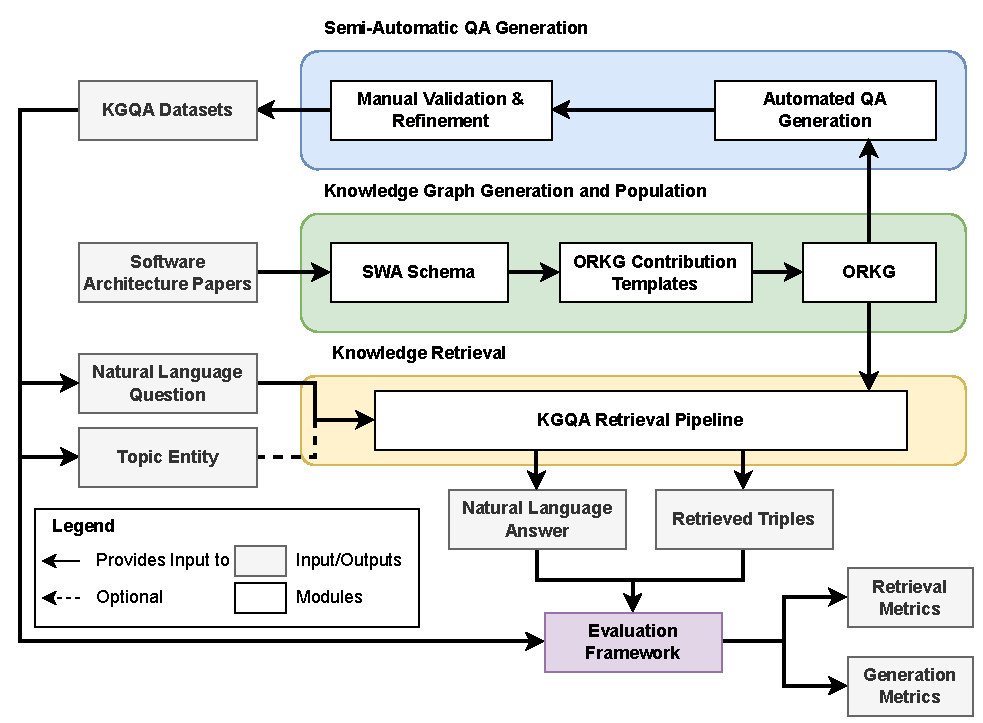
\includegraphics[width=0.95\textwidth]{figures/experiments/orkg/figures-imp_concept_exp.drawio.pdf}
    \caption[Evaluation Concept for Evaluating HubLink on the ORKG]{The overall evaluation concept that we used to perform the experiments on the \gls{orkg} using the proposed HubLink approach and the implemented \gls{kgqa} baseline approaches.}
    \label{fig:implementation_concept}
\end{figure}

This section details the evaluation concept, which we used to perform the evaluation with the objective of assessing the performance of our proposed HubLink approach. The primary objective of this concept is to systematically compare the capabilities of the HubLink retriever against established baseline methods. As indicated in Section~\ref{sec:implementation_orkg}, the \gls{orkg} serves as the underlying \gls{rkg} for these experiments. Furthermore, the \gls{karagen} method \cite{kaplan_combining_2024}, designed for implementing an \gls{llm}-based \gls{qa} system on the \gls{orkg}, forms the basis of the experimental setup. This framework is particularly suitable, as it encompasses the necessary components for applying a \gls{kgqa} retriever to the \gls{orkg}, including data population and retrieval processes. \autoref{fig:implementation_concept} provides a visual overview of the complete experimental design, which we detail in the following.

The general experimental concept starts with the \emph{Knowledge Graph Generation and Population} module. This module is proposed by the \gls{karagen} method and includes the preparation of contribution templates to populate the \gls{orkg} with data. We prepared four such templates, which are described in Section~\ref{sec:contribution_templates}. We fill these templates with data using the \gls{swa} schema detailed in Section~\ref{sec:implementation_orkg}. These populated templates are used by the \gls{sqa} system to automatically fill in the publication data in the \gls{orkg}.

The next module in the evaluation concept is \emph{Knowledge Retrieval}, which also aligns with the principles described in the \gls{karagen} method. In our implementation, the \gls{sqa} system is employed to construct the \gls{kgqa} retrieval pipeline. This enables systematic experimentation by providing a dynamic configuration setup where parameters and pipeline steps can be easily exchanged. The pipeline accepts a natural language question as input and, optionally, a topic entity serving as an entry point into the \gls{orkg}. It then performs knowledge retrieval utilizing either the HubLink retriever or one of five baseline \gls{kgqa} approaches from the literature, detailed in Section~\ref{sec:implementation_baselines}. The parameters that are used for these approaches are chosen by the \emph{Parameter Selection Process}, which is documented in \autoref{ch:parameter_selection_process}. The outputs of the \emph{Knowledge Retrieval} module are a natural language answer and the list of triples retrieved from the graph. These two types of outputs allow the evaluation of both the generation and the retrieval parts of the \gls{kgqa} approach.

The inputs to this system (question and topic entity) are automatically provided to the \gls{kgqa} approach by the \gls{kgqa} dataset. This dataset is the output of the \emph{Semi-Automatic QA Generation} module. Here, the \gls{qa} generation processes implemented in the \gls{sqa} system are used for the generation of \gls{kgqa} pairs (see Section~\ref{sec:implementation_qa_dataset_generation}). During generation, questions are generated in a controlled manner with \gls{llm} assistance using the \gls{orkg} subgraph as the data source. Furthermore, ground-truth data is generated, which is required for the subsequent evaluation phase.

Following the execution of the retrieval pipeline, the output is evaluated within the \emph{Evaluation Framework} module. This final module employs the generated ground-truth data to compute relevant performance metrics. Analysis of these metrics facilitates drawing conclusions regarding the effectiveness and performance characteristics of the evaluated \gls{kgqa} approaches.

\section{Software and Hardware Environment}
\label{sec:exp_prelim_environment}

In this section, we detail the environment in which the experiments for this thesis were executed.

The experiments were performed on the \gls{orkg} in the sandbox environment as detailed in Section ~\ref{sec:implementation_orkg}. However, this does not affect the generality of the results, as the \gls{orkg} serves as a representative example of an \gls{rkg} \cite{verma_scholarly_2023}. Consequently, the broader relevance of the obtained results are not compromised.

Moreover, all experiments were executed within the \gls{sqa} framework, which was developed by the author of the thesis and is detailed in Section~\ref{sec:implementation_sqa_framework}. Both the proposed HubLink retriever and the baseline retrievers were integrated into this framework. To ensure reproducibility, each experiment configuration is specified in a dedicated file using the JSON format. This facilitates straightforward replication of the experimental setup.

With respect to hardware, all experiments were performed in the same consistent hardware and software environment. The system operates on the Linux kernel version \emph{6.1.0-23-amd64}, equipped with a \emph{Intel(R) Xeon(R) Gold 6258R CPU @ 2.70GHz} processor and a \emph{Tesla V100S-PCIE-32GB} graphics processing unit. The implementation relies on a \emph{Python 3.12} environment, with a comprehensive list of software packages and their versions provided in the accompanying replication package \cite{schneider_replication_2025}.

Furthermore, the experimental setup uses both local and remote \glspl{llm}. Local LLMs are managed and executed via the Ollama framework\footnote{\url{https://ollama.com/} [last accessed on 24.02.2025]}. Remote access \glspl{llm} is facilitated through the OpenAI API\footnote{\url{https://platform.openai.com/docs/overview} [last accessed on 24.02.2025]}.


\section{Creating the KGQA Datasets}
\label{sec:implementation_qa_dataset_generation}

To be able to evaluate the retrieval capabilities on diverse retrieval operations and specific use cases in scholarly literature searches, we created new \gls{kgqa} datasets (\hyperref[enum:c3]{\textbf{C3}}). These datasets have been created with the help of the \gls{kgqa} retrieval taxonomy (\hyperref[enum:c3]{\textbf{C3}}) and six use cases using the semi-automatic generation procedures provided by the \gls{sqa} system (see Section~\ref{sec:qa_generator}).

In the following, we first introduce the use cases for scholarly literature search. Then, we explain the different levels of content granularity to clarify the level at which the new datasets are situated. Finally, we introduce the new \gls{kgqa} datasets for four different graph variants.

\subsection{Use Cases for Scholarly Literature Search}
\label{sec:qa_use_cases}

To create the \gls{kgqa} datasets, we prepared use cases. These use cases serve to support the creation process by incorporating real-world scenarios. To guide the development of use cases, we use the categories \emph{Answer Type} and \emph{Condition Type} from the \gls{kgqa} retrieval taxonomy introduced in \autoref{ch:question_catalog}. Here, \emph{Condition Type} refers to the types of conditions provided with a question. The \emph{Answer Type}, on the other hand, implicitly classifies the types of information expected in the answer.

For the design of the use cases, we decided to adapt these two categories to make them better suited to our experimental data. This decision was based on the fact that both categories originally included a large number of classes, which would result in an unmanageable number of use cases if all combinations were considered. Consequently, because the labeled data that we use consists of two types of data (metadata and content data), as shown in \autoref{tab:swa_data_schema}, we apply this distinction by adapting the answer and condition types for the creation of use cases. The result is the following adaptation of the two categories:

\begin{enumerate}[label={}, leftmargin=2.5em]
    \item \textbf{Adapted Answer Type} Classifies whether a question expects a \emph{metadata} or \emph{content data} type in the answer.
    \item \textbf{Adapted Condition Type} Classifies whether a question contains a condition of the \emph{metadata} or \emph{content data} type.
\end{enumerate}

Based on these adapted categories, we present six different use cases tailored to the scholarly literature search task.

\begin{tcolorbox}[title=Use Case 1] % Input:Metadata, Output: Metadata
The first use case reflects the current state of practice in scientific literature search. The researcher seeks additional details about the \emph{metadata} of one or more papers. To find this information, the researcher provides the \gls{kgqa} system with specific metadata information related to the papers they are interested in. In response, the \gls{kgqa} system returns information on other \emph{metadata} attributes of the papers rather than content information.
\end{tcolorbox}

The first use case is classified as \emph{Adapted Condition Type: Metadata} because all questions related to this use case require the answer to meet a specific metadata condition. Furthermore, this use case is categorized as \emph{Adapted Answer Type: Metadata}, as only metadata information is expected in the response.

A practical example of this use case would be a researcher asking for the publications of a specific author. In this case, the name of the author serves as the input constraint, while the returned publication titles represent the output type. Both the input and output consist solely of metadata. Similarly, another example would be a question that provides keywords. The \gls{kgqa} system then has to return the titles of the papers that are related to those keywords. 

Consequently, this use case reflects the current way of searching for scientific artifacts, since state-of-practice search engines like Google Scholar are expected to receive keywords and return titles of publications.

\begin{tcolorbox}[title=Use Case 2] % Input:Metadata, Output: Content
In the second use case, the researcher seeks information about the \emph{content} of one or more papers. In this use case, the researcher provides the \gls{kgqa} system with \emph{metadata} information about the papers and asks a question about their contents. The \gls{kgqa} system is then expected to extract content information related to specific papers that conform to the metadata constraints provided.
\end{tcolorbox}

The second use case is classified as \emph{Adapted Condition Type: Metadata}. However, its category regarding the second dimension is \emph{Adapted Answer Type: Content}, as the answer is expected to contain content information. From a retrieval perspective, we expect this use case to be more challenging, as it requires the \gls{kgqa} system to search through the extensive content information provided in the papers to find the expected answer.

A practical example of this use case would be a researcher asking for the conclusions that a specific publication has drawn. In this case, the name of the publication serves as the input constraint, where the \gls{kgqa} system is required to search the content of the specific publication. The expected output would be the conclusions drawn in the publication, which is content-based information as it requires the \gls{kgqa} system to reason over the content of the publication. Another scenario that would fit this use case would be a researcher asking the \gls{kgqa} system what research problems an author has worked on. In this case, it would require retrieving information from all publications of the author, extracting and aggregating the research problems that each publication investigated, and returning the aggregated list of research problems as the answer.

This use case shows the potential for \gls{kgqa} to help vastly improve the literature search process. By directly allowing researchers to find information based on the contents of a paper, the time and cognitive investment required to manually read through the text of the paper is reduced.

\begin{tcolorbox}[title=Use Case 3] % Input:Content, Output: Metadata
In the third use case, the researcher seeks information about \emph{metadata} of one or more papers. In this use case, the researcher provides the \gls{kgqa} system with \emph{content} constraints about the papers and asks a question about the metadata of the paper. The \gls{kgqa} system is then expected to extract metadata information related to the specific papers mentioned in the question.
\end{tcolorbox}

As opposed to the first two use cases, the third use case is classified as \emph{Adapted Condition Type: Content}. This is because the input constraint is based on content information. However, the expected answer is classified as \emph{Adapted Answer Type: Metadata}, as the answer is expected to only contain metadata information.

A practical example of this use case would be a researcher asking for publications that contain a specific evaluation method or treat the same research problem. Such a question would require inferring over the contents of publications to find out whether they have applied the provided evaluation method or whether they treat the same research problem. In this case, the expected output would be the titles of the publications, which is metadata information, whereas the input constraint is based on the type of expected answer.

This use case demonstrates the potential for improving the current document-centric literature search workflow. This is because a major difficulty faced by researchers is the identification of relevant publications that contain specific information. In the current workflow, researchers have to rely on metadata during their search. However, the desired information is often not explicitly stated in the title or abstract of the publication. Therefore, it is difficult to find the relevant publications using traditional search engines. Consequently, a \gls{kgqa} system that is able to find publications that contain specific content information would be a great improvement for the current literature research workflow.

\begin{tcolorbox}[title=Use Case 4]
In the fourth use case, the researcher seeks information about the \emph{content} of one or more papers. In this use case, the researcher provides the \gls{kgqa} system with content information about the paper, and asks a question about the \emph{content} of the paper. The \gls{kgqa} system is then expected to extract content information related to the specific papers mentioned in the question.
\end{tcolorbox}

The fourth use case has both the \emph{Adapted Condition Type} and \emph{Adapted Answer Type} classified as \emph{Content}. This is because both the input constraints and expected output types are based on content information. 

A practical example of this use case would be a researcher asking for common reference architectures that are proposed when tackling a specific research problem. In this case, the input constraint would be the research problem, while the expected output would be the reference architectures that are proposed in the literature. Both the input and output are content information, as they require reasoning over the content of the publications to find out which reference architectures are proposed for a specific research problem.

This use case is of particular interest when searching for definitions or explanations of specific concepts. In such cases, the location of the information in question is often uncertain, prompting the need to identify both the description and its source for the purpose of referencing it in another academic thesis.

\begin{tcolorbox}[title=Use Case 5]
In the fifth use case, a researcher seeks information about the \emph{content} of one or more papers. In this use case, the researcher provides the retriever with both \emph{metadata and content} information about the papers and asks a question about the content of the paper. The retriever is then expected to extract content information related to the specific papers mentioned in the question.
\end{tcolorbox}

The use cases until now only had a single type of input constraint. However, in the fifth use case, the input constraint is a combination of both \emph{metadata and content} information. This makes the task more difficult for the \gls{kgqa} system. It is now required to search for two different constraint types that might even be stored in different locations in the underlying \gls{kg}. The expected output is \emph{Adapted Answer Type: Content} as the answer is expected to contain content information. 

Practical examples include combinations of the second and fourth use cases. For example, a researcher could ask for a summary of conclusions that publications have drawn in a specific time frame for a specific research problem. In this case, the input constraint would be the research problem and the time frame, which are content and metadata information, respectively. The expected output would be the summary of conclusions that are drawn in the publications, which is content information. 

This use case is particularly interesting in scenarios where a researcher wants to save time by not reading the full text of a publication. Instead of reading the text, the researcher can pose questions to the document in order to retrieve the necessary information.

\begin{tcolorbox}[title=Use Case 6]
In the sixth use case, the researcher seeks information about \emph{metadata} of one or more papers. In this specific use case, the researcher provides the retriever with both \emph{metadata and content} information about the papers, such as the name of an evaluation method and the year of publication, and asks a question about the metadata of the papers. The retriever is then expected to extract metadata information related to the specific papers mentioned in the question.
\end{tcolorbox}

The sixth use case has the same \emph{Adapted Condition Types} as the fifth use case, but the second dimension is \emph{Adapted Answer Type: Metadata} as the answer is expected to contain metadata information. 

The practical examples of this use case are a mixed version of the first and third use cases. For example, a researcher could request publications that have applied a specific evaluation method in a specific research field. In this case, the input constraint would be the evaluation method and the research field, which are content and metadata information, respectively. The expected output would be the titles of publications that have applied the evaluation method in the research field, which is metadata information.

\textit{Note that, as evident from the aforementioned use cases, the Answer Type dimension is not being mixed. According to the \gls{kgqa} retrieval taxonomy, such a question would be designated as a Multiple Intentions question. Splitting this question into two distinct questions is a viable approach to enhance clarity and manage complexity. However, in the interest of maintaining manageable complexity, the multiple intentions are not being considered in the use cases.}

\subsection{Overview of Content Granularity}
\label{sec:content_granularity}

When creating datasets, it is useful to classify the level of granularity the data contains. This helps to provide a better understanding of the content of the dataset. For this purpose, we introduce four levels of granularity, which differ in their degree of abstraction:

\begin{enumerate} 
    \item \textbf{Document-based:} The current standard for distributing literature online. Publications are stored as PDF files in a database together with their metadata. Users locate publications using the metadata and then extract relevant information from the documents themselves by reading the provided texts. 
    \item \textbf{Chunk-based:} Originating from \gls{rag} \cite{lewis_retrieval-augmented_2021}, this approach divides documents into smaller chunks and embeds them into a vector space. Relevant chunks are retrieved from the database using nearest-neighbor search queries.
    \item \textbf{Statement-based:} Here, concise summaries or statements are extracted from publications and stored directly in a database. 
    \item \textbf{Label-based:} The highest level of abstraction, where publications are classified using labels, which may include hierarchical structures. These labels give readers a quick overview of the content of a publication. 
\end{enumerate}

Using this classification, we assign the datasets that we used for our experiments to the \emph{Label-based} abstraction level. This is because they consist of extracted terms structured according to a predefined schema as defined in \autoref{tab:swa_data_schema}.

\subsection{Dataset Creation Process}
\label{sec:label_based_qa_dataset}

Contribution \textbf{C2} of this thesis are \gls{kgqa} datasets, which we used to carry out the experiments. These \gls{kgqa} datasets were created using the data from the publication dataset introduced in Section~\ref{sec:experiments_dataset}. For their creation, the data was first loaded into the \gls{orkg}, and then \gls{kgqa} pairs were generated using the semi-automated \gls{kgqa} generation strategy described in Section~\ref{sec:qa_generator}. In the following, we present the creation process and the key characteristics of these datasets.

\subsubsection{Dataset Structure} 

The datasets consist of \gls{kgqa} pairs. Each pair includes the question itself together with the corresponding \emph{ground-truth} data. This data is used during the evaluation to determine whether the answer and the data retrieved by the \gls{kgqa} approach are correct. In this context, the ground truth represents one possible valid answer to the question, as well as a collection of triples needed to answer it. In addition to the question and the ground truth, each \gls{kgqa} pair also includes further metadata. This encompasses a \emph{topic entity} that can serve as an entry point into the graph for the retriever, the \glspl{doi} of the papers referenced in the question, and the template used to generate the question. The pairs are also classified according to use case, semi-typed nature, and the categories defined in the taxonomy.

\subsubsection{Question Diversity}

To ensure that the questions in the \gls{kgqa} datasets exhibit a high degree of variability that allows meaningful conclusions about the capabilities of a \gls{kgqa} system, we structured the datasets considering multiple dimensions. First, we use the \emph{use cases} described in Section~\ref{sec:qa_use_cases} to map each question to a realistic application scenario. During the creation phase, we assigned questions to each of the six use cases to ensure a balanced distribution between them. To further reflect the retrieval capabilities required for each question, we incorporated the \emph{Retrieval Operation} category from the \gls{kgqa} retrieval taxonomy introduced in \autoref{ch:question_catalog}. Each question is assigned to a specific retrieval operation, ensuring that operations are covered evenly. 

Additionally, the dataset distinguishes between \emph{untyped} and \emph{semi-typed} questions. This distinction is meant to assess how well a retriever can handle synonyms or missing type information:

\begin{itemize}
    \item \textbf{Semi-Typed Questions} Each question in the dataset targets specific triples in the \gls{kg}, with each triple consisting of a subject, predicate, and object. Depending on the triple, either the subject or the predicate may carry type information about the object. For example, the requested triple $(Research Object Entity, Name, Reference Architecture)$, requires the question to specify that the reference architecture is a research object.
    
    \item \textbf{Untyped Questions} In contrast, \emph{untyped} questions do not include the type information. Using the same example, the question would simply ask about the reference architecture without stating that it is a research object. This increases the difficulty of retrieval because the retriever must infer the object type based solely on the object name.
\end{itemize}


\subsubsection{Restrictions} 

To keep the datasets manageable in terms of complexity, certain constraints were applied during the creation. First, the number of golden triples needed to answer a question was limited to a maximum of 10. This limitation ensures that questions do not require information spread across the entire dataset. Without this restriction, answering broad questions would require extensive aggregation, resulting in runtimes that are too long for the scope of a master thesis.

Furthermore, it is essential that the retriever parameters are set in such a way that the retrievers can fully answer the given questions. By limiting the number of golden triples, we can ensure that this is the case. Consequently, the chosen threshold of 10 represents a compromise between the efficiency of the retrievers and the expressiveness of the questions. A higher threshold would require increasing retriever parameters, such as maximum depth or width, leading to longer runtimes. A lower threshold, on the other hand, would reduce the informativeness of the questions or even make some of them unanswerable. Therefore, selecting a limit of ten triples strikes a balance between maintaining acceptable runtimes and preserving the relevance and feasibility of the questions.

\begin{table}[t]
\centering
\begin{tabular}{lccccccc}
\toprule
\textbf{} & \multicolumn{6}{c}{\textbf{Use Cases}} \\
\cmidrule(lr){2-7}
\textbf{Retrieval Operation} & \textbf{1} & \textbf{2} & \textbf{3} & \textbf{4} & \textbf{5} & \textbf{6} \\
\midrule
aggregation   & 4 & 4 & 4 & 4 & 4 & 4 \\
basic         & 4 & 4 & 4 & 1 & 4 & 1 \\
comparative   & 4 & 4 & 4 & 4 & 4 & 4 \\
counting      & 4 & 4 & 4 & 4 & 4 & 4 \\
negation      & 0 & 0 & 4 & 4 & 4 & 4 \\
ranking       & 4 & 4 & 4 & 4 & 4 & 4 \\
relationship  & 4 & 4 & 4 & 4 & 4 & 4 \\
superlative   & 0 & 0 & 4 & 4 & 4 & 4 \\
\bottomrule
\end{tabular}
\caption[Distribution of Question Templates]{Distribution of question templates across the use case and retrieval operation dimensions.}
\label{tab:distribution_of_question_templates}
\end{table}

\subsubsection{Template Questions} 

To utilize the semi-automatic \gls{kgqa} generation described in Section~\ref{sec:qa_generator}, template questions are required. For the datasets, a total of 170 different template questions were created manually, the full list of which is available in our replication package (see \cite{schneider_replication_2025}). As mentioned previously, these questions were diversified along the dimensions of the use case and retrieval operation. The precise distribution of these template questions is shown in \autoref{tab:distribution_of_question_templates}. For most combinations of use case and retrieval operation, four template questions were generated, although there are some exceptions. Specifically, for the use cases four and six, only two suitable examples were found for the \emph{Basic} operation. Additionally, for use cases one and two, no suitable template questions were identified for the \emph{Negation} and \emph{Superlative} classes that were meaningful and below the threshold of ten golden triples.

Regarding the semi-typed nature of the questions, the dataset contains 86 semi-typed and 84 untyped questions. Generally, an equal number of semi-typed and untyped questions were created for each combination of use case and retrieval operation, with the exception of the individual questions for use cases four and six as mentioned above.

\subsubsection{Classification According to KGQA Retrieval Taxonomy} 

According to the classification following the \gls{kgqa} retrieval taxonomy described in \autoref{ch:question_catalog}, the distribution is as follows: Within the \emph{Condition Type} category, 133 questions were classified as \emph{Named Entity} and 37 as \emph{Named Entity, Temporal}. This indicates that two types of constraints must be considered by the retriever: either solely the consideration of a named entity or additionally a temporal constraint.

For the \emph{Answer Format} category, the dataset comprises 61 \emph{Enumerative}, 58 \emph{Simple}, and 51 \emph{Explanatory} questions. The classification according to \emph{Graph Representation} shows that 152 questions belong to the \emph{Multi-Fact} type, meaning they require multiple triples for their answer, while 18 questions are categorized as \emph{Single-Fact}, requiring only one triple.

In the \emph{Answer Type} category, 86 questions expect an answer of type \emph{Named Entity}, 20 questions require a \emph{Quantitative} answer, two questions anticipate a \emph{Boolean} answer, and two additional questions have an \emph{Other Type} of response. Furthermore, the dataset includes questions with more complex answer types: 24 questions expect either \emph{Description} combined with \emph{Quantitative} (\emph{Description, Quantitative}) or \emph{Description} with \emph{Named Entity} (\emph{Description, Named Entity}). Additionally, 13 questions require answers of the type \emph{Description, Quantitative, Temporal}, and 8 questions expect answers of the type \emph{Description, Named Entity, Temporal}, which means that they also require a year.

With respect to the \emph{Intention Count} category, the dataset exclusively contains \emph{Single Intention} questions, as multiple intentions were not considered. For the \emph{Question Goal} category, due to insufficient variability in the publication data, only the class \emph{Information Lookup} applies. Regarding \emph{Answer Credibility}, all the questions meet the \emph{Objective} criterion.

\subsubsection{Dataset Creation} 
To generate the datasets, we used the semi-automatic cluster and subgraph-based generation methods introduced in Section~\ref{sec:qa_generator}. Based on the template question and the provided generation methods, we generated a total of 170 initial questions for the graph variant \hyperref[enum:gv2]{\textbf{GV2}}. Then, each question and the corresponding ground truth were reviewed manually to ensure that both the question and the generated golden answers are consistent and grammatically correct. To further ensure quality, an additional \gls{llm}-based feedback script was employed, which checked each question and answer to provide feedback for changes if necessary.

After the quality of each question-answer pair was verified, we manually classified each question with the remaining categories of the \gls{kgqa} retrieval taxonomy. Then, we employed the \emph{conversion} scripts introduced in Section~\ref{sec:orkg_ensuring_repeatability} to generate the \gls{kgqa} datasets for the graph variants \hyperref[enum:gv1]{\textbf{GV1}}, \hyperref[enum:gv3]{\textbf{GV3}}, and \hyperref[enum:gv4]{\textbf{GV4}}.




\section{Evaluation Framework and Metrics}
\label{sec:exp_prelim_evaluation_framework}

The \gls{kgqa} approaches that we are testing in our thesis conform to the principles of \gls{rag}, because they retrieve information that is then used to improve the generation of an answer. Consequently, we employ an evaluation framework for \gls{rag}-based systems. A popular framework is \gls{rgar} \cite{yu_evaluation_2024}, which will serve as the basis for structuring our evaluation. The framework is divided into three modules. The first module, called \emph{Evaluation Target}, defines the direction of the evaluation. The second module is \emph{Evaluation Dataset}, which outlines how the datasets were created and selected. The last module is \emph{Evaluation Metric}, which presents the specific metrics used to evaluate the targets based on the datasets. 

In the following, we first introduce the evaluation targets differentiating between retrieval and generation objectives. Then, we briefly explain the datasets that were applied in the experiments. Finally, we introduce the \gls{gqm} plan that shows how each target is evaluated using specific questions and metrics.


\subsection{Evaluation Targets}
\label{sec:evaluation_targets}

This section introduces the evaluation targets, which are the constructs intended to be evaluated during the evaluation. Each evaluation target is defined using \glspl{eo} and \glspl{gt}.

\subsubsection{Outputs and Ground Truth}

\glspl{eo} are the actual outputs of the \gls{kgqa} approach, while \glspl{gt} are the expected outputs as defined in the \gls{kgqa} dataset. We define the following \glspl{eo} and \glspl{gt} for our evaluation:

\begin{enumerate}[label={}, leftmargin=5em]
    \item[\textbf{EO1}] \label{enum:eo1} Retrieved Triples
    \item[\textbf{EO2}] \label{enum:eo2} Generated Answer
    \item[\textbf{GT1}] \label{enum:gt1} Golden Triples
    \item[\textbf{GT2}] \label{enum:gt2} Golden Answer
\end{enumerate}

Each \gls{kgqa} approach returns two types of outputs in our setting. The first output is \textbf{EO1}, which represents the triples that have been retrieved from the \gls{orkg} and rated by the approach as relevant to answering the provided question. Second, \textbf{EO2} is the answer that has been generated by an \gls{llm} based on the retrieved triples and the question.

To evaluate the outputs of the retriever, the \gls{kgqa} dataset provides two types of ground truth data. First, \textbf{GT1} are the golden triples, which are exactly those triples that are required to fully answer the question that was asked. Consequently, the retriever has to find all golden triples to be entirely successful at the retrieval task. Second, \textbf{GT2} is a golden answer formulated in natural language, which provides a response to the question and is based on the golden triples. 

\subsubsection{Evaluation Targets}
The combination of \glspl{eo} and \glspl{gt} generates the evaluation targets, which are subdivided into targets for retrieval (\emph{ReT}) and for generation (\emph{GeT}):

\begin{enumerate}[label={}]
    % Triples to Golden Triples
    \item \textbf{ReT1}\label{enum:ret1} EO1 \(\leftrightarrow \) GT1
     % Gen Answer to Golden Answer
    \item \textbf{GeT1}\label{enum:get3} EO2 \(\leftrightarrow \) GT2
    % Gen Answer to Question
    \item \textbf{GeT2} \label{enum:get1} EO2 \(\leftrightarrow \) Question
    % Gen Answer to Triples
    \item \textbf{GeT3} \label{enum:get2} EO2 \(\leftrightarrow \) GT1
\end{enumerate}

The targets introduced above guide the evaluation process. The retrieval target (\hyperref[enum:get1]{\textbf{ReT1}}) assesses the effectiveness of the context retrieval phase by comparing the retrieved triples (\hyperref[enum:eo1]{\textbf{EO1}}) with the golden triples (\hyperref[enum:gt1]{\textbf{GT1}}). This evaluation focuses on accuracy, relevance, and robustness. Here, accuracy is about the extent to which the retrieval approach is capable of fetching the desired triples (\hyperref[enum:get1]{\textbf{GT1}}) from the graph. Relevance refers to the degree to which the retrieved triples (\hyperref[enum:get1]{\textbf{EO1}}) correspond to the golden triples (\hyperref[enum:get1]{\textbf{GT1}}), where more irrelevant triples result in lower overall relevance. Finally, robustness refers to the ability of the retrieval system to maintain consistent performance in terms of accuracy and relevance despite variations encountered in the complexity of input questions (e.g., phrasing, the presence or absence of explicit type information, diverse use case requirements, and structural or lexical variability) across different knowledge graph schemas. The general intent behind \hyperref[enum:get1]{\textbf{ReT1}} is therefore to quantify how well the retriever identifies the correct information and how resilient its performance is under various operational conditions.

With regard to the generation targets, \hyperref[enum:get1]{\textbf{GeT1}} evaluates the quality of the generated answer by assessing its semantic and factual alignment with the reference ground truth answer (\hyperref[enum:get1]{\textbf{GT2}}). This target aims to measure how closely the generated answer of the system (\hyperref[enum:get1]{\textbf{EO2}}) matches an ideal and correct answer derived from the ground truth. The focus is on both the meaning and the accuracy of the information presented. High performance on this target indicates that the system can produce answers that are similar to a known correct answer.

\hyperref[enum:get2]{\textbf{GeT2}} evaluates how well the generated answer (\hyperref[enum:get1]{\textbf{EO2}}) aligns with the intent and content requirements of the input question. This involves assessing whether the answer directly addresses the topic posed by the question and fulfills any specific instructions or constraints given, such as performing a ranking or counting operation. Consequently, this target measures the usefulness and appropriateness of the generated answer in the context of the question.

Finally, \hyperref[enum:get3]{\textbf{GeT3}} evaluates the faithfulness and adherence to the source material of the generated answer (\hyperref[enum:get1]{\textbf{EO2}}) relative to the retrieved triples (\hyperref[enum:get1]{\textbf{EO1}}). It evaluates whether the statements and claims made in the generated answer accurately and exclusively reflect the information present within the retrieved triples. 

\subsection{Evaluation Datasets}
\label{sec:evaluation_datasets}

To evaluate the defined targets, datasets are needed to conduct the experiments. In Section~\ref{sec:implementation_qa_dataset_generation} we document the creation of \gls{kgqa} datasets. These datasets have been used to conduct the experiments and evaluate the targets.

\subsection{Evaluation Plan}
\label{sec:evaluation_goals_and_metrics}

This section details the evaluation plan designed to assess the performance of the proposed HubLink system against baseline approaches. Following the introduction of the evaluation targets in Section~\ref{sec:evaluation_targets}, we adopt the \gls{gqm} method \cite{basili_methodology_1984,basili_software_1992}. Consequently, we present a detailed \gls{gqm} plan that systematically links each evaluation target (serving as a goal) with specific questions, which are in turn addressed using a defined set of quantitative metrics. To aggregate the metrics across all questions, we are using the \emph{macro-averaging} strategy (see Section~\ref{sec:fundamentals_evaluation_rag}) because it attributes equal weight to each individual question without favoring those questions that request more triples.

In the following, we present each of the goals with their corresponding set of questions and metrics. We begin with the retrieval, followed by the generation.



\subsubsection{Evaluation of the Retrieval Performance} 

The initial evaluation target, \hyperref[enum:ret1]{\textbf{ReT1}}, centers on assessing the relevance and robustness of the contexts retrieved by HubLink. Several questions arise from this goal, evaluated using a suite of seven metrics. Standard information retrieval metrics, namely \emph{Precision}, \emph{Recall}, and \emph{F1} are calculated based on the formulas presented by \textcite{yu_evaluation_2024}. The determination of \gls{tp}, \gls{fp}, and \gls{fn} involves comparing the triples retrieved by the system with the ground-truth triples provided within the reference \gls{kgqa} dataset. The \emph{Accuracy} metric is omitted from this evaluation, as its calculation requires knowledge of \gls{tn}, which requires a complete listing of all irrelevant contexts, which is not available in our \gls{kgqa} datasets.

To evaluate the ability of the retriever to rank relevant contexts highly, rank-aware metrics are incorporated. Specifically, \emph{MAP@k} and \emph{MRR@k} are adapted from the implementations of \textcite{tang_multihop-rag_2024}. The \emph{Hits@k} metric is implemented following the definition provided by the AmpliGraph library\footnote{\url{https://docs.ampligraph.org/en/1.2.0/generated/ampligraph.evaluation.hits_at_n_score.html} [last accessed on 17.01.2025]}. In addition, \emph{EM@k} is included, calculated according to the definition of \textcite{ibrahim_survey_2024}. 

With regard to the required parameter $k$ that determines the number of top contexts considered, we have set this parameter to 10. This choice reflects the maximum number of ground truth triples associated with any single question in our \gls{kgqa} datasets, as detailed in Section~\ref{sec:label_based_qa_dataset}.

Furthermore, we test the environmental impact of the retrieval using the absolute, relative, and delta carbon emissions using the metrics specified by \cite{kaplan_responsible_2025}. The tracking of the emissions is facilitated by the Codecarbon library\footnote{\url{https://github.com/mlco2/codecarbon} [Accessed: 2025-01-17]}, which tracks the \emph{CPU Energy Consumption}, \emph{GPU Energy Consumption}, and \emph{RAM Energy Consumption}, measured in watts and then converts those measurements to estimate the total \emph{Carbon Emissions} as \(CO_2\) equivalent. Moreover, to evaluate runtime and token costs, we measure \emph{System Latency} as the total time taken to retrieve the context and generate an answer while also tracking the number of \emph{LLM Tokens} consumed during the retrieval and generation phases.


% Beyond the \gls{gqm} framework, several measurements are tracked to quantify practical operational aspects. \emph{System Latency} is measured as the total time elapsed to retrieve the context and generate an answer. Sustainability considerations are addressed by tracking energy consumption, specifically \emph{CPU Energy Consumption}, \emph{GPU Energy Consumption}, and \emph{RAM Energy Consumption}, measured in watts. These energy measurements are aggregated to estimate the total \emph{Carbon Emissions} as \(CO_2\) equivalent. The tracking of energy and emissions is implemented using the Codecarbon library\footnote{\url{https://github.com/mlco2/codecarbon} [Accessed: 2025-01-17]}. Finally, the computational cost associated with the usage of the \gls{llm} is monitored by tracking the number of \emph{LLM Tokens} consumed during the retrieval and generation phases.


\subsubsection{Evaluation of the Generation Performance}

Transitioning to answer generation, the target \hyperref[enum:get1]{\textbf{GeT1}} focuses on comparing the factual and semantic similarity between the generated answer of the \gls{kgqa} approach and the golden answer in the \gls{kgqa} dataset. Lexical similarity is measured using \emph{BLEU}\footnote{\url{https://pypi.org/project/sacrebleu/} [last accessed on 17.01.2025]} and \emph{ROUGE}\footnote{\url{https://pypi.org/project/rouge-score/} [last accessed on 17.01.2025]}, employing their respective standard Python implementations. Semantic similarity is assessed using \emph{BertScore}\footnote{\url{https://github.com/Tiiiger/bert_score} [last accessed on 17.01.2025]} utilizing the official implementation that provides Precision, Recall, and F1 variants based on contextual embeddings. Further evaluation leverages \gls{llm}-as-a-judge metrics provided by the RAGAS framework\footnote{\url{https://github.com/explodinggradients/ragas} [last accessed on 17.01.2025]}. This includes \emph{Factual Correctness}, where an \gls{llm} decomposes both the generated and reference answers into claims to calculate Precision, Recall, and F1 based on the comparisons of those claims \cite{es_ragas_2023}. We further use the \emph{Semantic Similarity} metric, which calculates the cosine similarity and the \emph{String Similarity} metric, which calculates the Levenshtein distance between the generated answer and the golden answer. Both metrics are also provided by the RAGAS framework.

The subsequent generation target, \hyperref[enum:get2]{\textbf{GeT2}}, addresses the alignment of the generated answers with the intent of the question, encompassing both semantic content and instructional constraints. This target involves two specific questions. The first, referring to semantic alignment, is evaluated using the \emph{Answer Relevancy} metric from RAGAS. This metric uses an \gls{llm} to generate plausible questions based solely on the generated answer and then measures the semantic similarity (cosine similarity) between these generated questions and the original question \cite{es_ragas_2023}. The rationale is that a relevant answer should allow an accurate reconstruction of the original query. The second question, which focuses on adherence to instructional intent (e.g., performing a ranking task as requested), is assessed using a custom implementation that we developed on our own. In this process, an \gls{llm} evaluates the generated answer against the specific instructions embedded within the question to determine the degree of compliance.

The final generation target \hyperref[enum:get3]{\textbf{GeT3}} concerns the faithfulness of the generated answer to the information contained within the retrieved contexts. This is evaluated using the \emph{Faithfulness} metric from the RAGAS framework. This metric utilizes an \gls{llm} to break down the generated answer into individual statements and verifies each statement against the provided retrieved context  \cite{es_ragas_2023}. This means that the metric evaluates whether the answer was actually derived from the context or from the internal knowledge of the \gls{llm}. We use this to evaluate whether the triples that were retrieved are actually reflected in the generated answer. 

\vspace{\medskipamount}
{\large\textbf{Goal-Question-Metric Plan:}} 
\label{sec:evaluation_gqm_plan}

\textbf{Ret1} Assess the relevance and robustness of retrieved contexts in scholarly literature search.
\begin{enumerate}[label={}]
    \item \textbf{Q1} To what extent does the HubLink retrieval algorithm improve context relevance and accuracy compared to baseline KGQA methods in scholarly literature search?
    \begin{enumerate}[label={}]
        \item \textbf{M1.1} Precision, \textbf{M1.2} Recall, \textbf{M1.3} F1, \textbf{M1.4} Hits@k, \textbf{M1.5} EM@k, \textbf{M1.6} MRR@k, \textbf{M1.7} MAP@k
    \end{enumerate}
    \item \textbf{Q2} How does retrieval performance vary with the complexity of operations required by different scholarly questions?
    \begin{enumerate}[label={}]
        \item \textbf{(see Q1.1)}
    \end{enumerate}
    \item \textbf{Q3} How does retrieval performance vary across distinct scholarly literature-search use cases?
    \begin{enumerate}[label={}]
        \item \textbf{(see Q1.1)}
    \end{enumerate}
    \item \textbf{Q4} What impact does the presence or absence of explicit type information in questions have on the retrieval performance?
    \begin{enumerate}[label={}]
        \item \textbf{(see Q1.1)}
    \end{enumerate}
    \item \textbf{Q5} How robust is the proposed approach to structural and lexical variability across alternative knowledge graph schema representations?
    \begin{enumerate}[label={}]
        \item \textbf{(see Q1.1)}
    \end{enumerate}
    \item \textbf{Q6} How efficient is the proposed approach considering runtime and language model tokens required when compared to baseline KGQA methods?
    \begin{enumerate}
        \item \textbf{M1.8} Runtime per question, \textbf{M1.9} LLM tokens per question
    \end{enumerate}
    \item \textbf{Q7} How does the proposed approach compare with regard to the environmental impact when compared to baseline KGQA methods?
    \begin{enumerate}
        \item \textbf{M1.10} Absolute carbon emissions, \textbf{M1.11} Relative carbon emissions, \textbf{M1.12} Delta carbon emissions
    \end{enumerate}
\end{enumerate}
% 
\textbf{GeT1} Evaluate how well the generated answer aligns semantically and factually with reference answers.
\begin{enumerate}[label={}]
    \item \textbf{Q8} How semantically and factually consistent are the generated answers of the proposed approach when compared to answers generated by baseline KGQA approaches?
    \begin{enumerate}[label={}]
        \item \textbf{M2.1} BLEU, \textbf{M2.2} ROUGE, \textbf{M2.3} Semantic Similarity, \textbf{M2.4} String Similarity, \textbf{M2.5} Bert Precision, \textbf{M2.6} Bert Recall, \textbf{M2.7} Bert F1, \textbf{M2.8} Factual Correctness Precision, \textbf{M2.9} Factual Correctness Recall, \textbf{M2.10} Factual Correctness F1 \\
    \end{enumerate}
\end{enumerate}
%
\textbf{GeT2} Evaluate how well the generated answer aligns with the intent and content of the question.
\begin{enumerate}[label={}]
    \item \textbf{Q9} To what extent do the answers generated by HubLink reflect the semantic intent of scholarly questions when compared to baseline KGQA approaches?
    \begin{enumerate}[label={}]
        \item \textbf{M3.1} Answer Relevancy
    \end{enumerate}
    \item \textbf{Q10} To what extent do the generated answers follow the instructional expectations of scholarly questions when compared to baseline KGQA approaches?
    \begin{enumerate}[label={}]
        \item \textbf{M3.2} Instruction Following
    \end{enumerate}
\end{enumerate}
% 
\textbf{GeT3} Evaluate how well the generated answer aligns with the retrieved context.
\begin{enumerate}[label={}]
    \item \textbf{Q11} To what extent are generated answers of HubLink faithful to the retrieved context and free from unsupported claims when compared to baseline KGQA approaches?
    \begin{enumerate}[label={}]
        \item \textbf{M4.1} Faithfulness
    \end{enumerate}
\end{enumerate}





\section{Dependent and Independent Variables}
\label{sec:exp_prelim_variables}
This section describes the independent and dependent variables of our experiments.

\paragraph{Independent Variables:} These variables encompass the specific experimental configurations that are systematically varied between runs while performing the evaluation. The key independent variables include the choice of the core retrieval algorithm, modifications to its parameters, the specific dataset used for evaluation, the underlying knowledge base, and the selected \gls{llm}. These variables represent the factors that are manipulated to observe their effect on overall performance.

\paragraph{Dependent Variables:} The dependent variables represent those constructs that we are interested in improving. Consequently, these constitute the quantitative performance measures used to assess the outcomes of different experimental configurations and directly correspond to the metrics detailed in the evaluation plan (see Section~\ref{sec:evaluation_goals_and_metrics})

The experimental methodology involves the execution of a series of tests in which specific configurations of independent variables (pipeline components and parameters) are applied. For each configuration, the dependent variables (retrieval, generation, and operational metrics) are measured. The primary objective of this process is to analyze the collected data to determine the influence of variations in the independent variables on the observed system performance in the different categories of dependent variables. Because each \gls{kgqa} approach has a different set of parameters (independent variables), we employ a \emph{Parameter Selection Process} to choose the appropriate values for our subsequent experiments. The selection process is documented in the following \autoref{ch:parameter_selection_process}.






\chapter{Parameter Selection Process}
\label{ch:parameter_selection_process}

The HubLink and the baseline approaches each expose a variety of parameters that, in an ideal scenario, would be optimized via a full hyperparameter-tuning procedure using separate training and test datasets. However, we deviate from this optimal approach due to practical constraints, as we found that experiments with \glspl{llm} are both costly and time-consuming. Since the durations of multi-week experiments fall outside the scope of this master thesis, we adopt an alternative workflow we refer to as the \emph{Parameter Selection Process}. The goal of this process is to determine the parameter configurations that optimize the retrieval performance of the \gls{kgqa} retrievers in our experimental setting while respecting the time and resource constraints of this project. Consequently, the results of this process are configurations for each retriever, which we then used in our experiments.

The following sections are organized as follows. First, in Section~\ref{sec:selection_planning}, we explain the planning process that was done prior to conducting the selection process. Then, Sections \ref{sec:param_selection_hublink}, \ref{sec:param_selection_difar}, \ref{sec:param_selection_fidelis}, and \ref{sec:param_selection_mindmap}, describe the selection process for HubLink and the baseline retrievers: DiFaR, FiDeLiS, and Mindmap. Finally, in Section~\ref{sec:param_selection_threats_to_validity}, we discuss threats to the validity of the parameter selection process.




\section{Planning}
\label{sec:selection_planning}

This section documents the planning of the parameter selection process. We first describe the methodology that was applied to realize the process. Next, we explain why we chose the Recall and Hits@10 metrics for the selection. Following this, we describe the dataset that was applied and the \glspl{llm}. Then, we describe the preliminary pipeline steps that are implemented before we describe why we decided to omit the StructGPT and ToG \gls{kgqa} approaches.

\subsection{Methodology}
\label{sec:selection_planning_methodology}

To carry out this process, we apply the \gls{ofat} method to identify the best parameters according to the Recall and Hits@10 metrics. In this method, a base configuration is selected and then each factor is successively varied over its range while all other factors are kept constant \cite{montgomery_design_2017}. Consequently, we defined a base configuration and a range of parameter values for each \gls{kgqa} approach. Then, following the \gls{ofat} method, multiple run configurations have been created based on the base configuration and ranges to subsequently test them using a reduced version of the \gls{kgqa} dataset.


\subsection{Metrics for Selection}
\label{sec:selecting_tuning_metric}

To conduct the selection, metrics need to be chosen that allow us to determine whether a change in the value of a parameter is justified. For the selection process, we focused on retrieval performance rather than generation. This is because the generation of the answers depends on the retrieved contexts, which means that if the retriever cannot find the contexts that are relevant, it will not be able to generate an answer based on it. With regard to the choice of retrieval metrics, our primary metric is Recall, although we also use Hits@10 where needed. There are several reasons for these metrics, which we explain in the following:

First, when constructing the \gls{kgqa} datasets (see Section~\ref{sec:implementation_qa_dataset_generation}), we ensured that only those triples were designated as the ground truth for which the content required to answer the question is actually present. We deliberately omitted any intermediate triples that must be traversed to reach the target since they are not strictly necessary to answer the actual question. To illustrate, consider a question that is asking for the authors of a paper. The authors are stored in separate nodes that all connect to a root node named \emph{Authors List}. That root node serves only as a means to reach the author nodes and does not provide the information necessary to answer the question. In our preliminary tests, we observed that retrievers tend to include such intermediate nodes in their retrieved context. Furthermore, because answer generation occurs after context retrieval, these nodes could be helpful during answer generation by providing additional context to the \gls{llm}. Consequently, we chose not to penalize this behavior, which is consistent with using the Recall metric.

With regard to the Hits@10 metric, this metric allows us to understand whether the retriever ranks those contexts that are more relevant higher than those that are less relevant. For example, if the retriever includes intermediate triples in their output, the Hits@10 metric is still maximal if those triples that are actually relevant are higher on the list of outputs.

\subsection{Choosing a Graph Variant}
\label{sec:selection_planning_graph_variant}

In Section~\ref{sec:contribution_templates} we introduced four different graph variants for our experiments to test the robustness of \gls{kgqa} approaches. However, due to cost reasons, we were unable to run the parameter selection process (and experiments) on all four graph variants. We therefore decided on \hyperref[enum:gv1]{\textbf{GV1}} as we believe that it is the graph variant with the most realistic modeling for real-world scenarios. The reason for this is that long paths allow the relationships between information to be captured, which preserves crucial context. Furthermore, the content is distributed by concern, which allows for extensibility in the future.

\subsection{Using a Reduced KGQA Dataset}
\label{sec:selection_planning_reduced_qa}

In addition to only running the selection process on one graph variant as mentioned above, we used a reduced version of the label-based \gls{kgqa} dataset (for \hyperref[enum:gv1]{\textbf{GV1}}) during the selection process. As described in Section~\ref{sec:implementation_qa_dataset_generation}, the \gls{kgqa} datasets were created with respect to use cases and retrieval operations. Each question is also classified as either semi-typed or untyped. For almost any pairing of a use case with a retrieval operation, there are four corresponding pairs of questions and answers. When constructing the reduced dataset, we therefore selected one semi-typed question per combination to ensure that each question is representative of the larger dataset. We chose semi-typed over untyped questions, as we expected them to perform better, which is important when selecting parameters. Consequently, the reduced \gls{kgqa} dataset for graph variant \hyperref[enum:gv1]{\textbf{GV1}} contains a total of 44 questions.



% We created \textbf{GV1} in such a way that it provides continued value for future use. This means that it should be easy to read and extendable for future contexts. 

% We gathered the majority of our results using graph variant \hyperref[enum:gv1]{\textbf{GV1}} as we expect \hyperref[enum:gv1]{\textbf{GV1}} to be the most relevant model for real-world scenarios due to its inherent extendability and its capability to capture semantic relationships. We explicitly state in each following section which graph variants we employed for the presented results.

\subsection{Large Language and Embedding Models}
\label{sec:selection_planning_llms}

As all retrievers are based on \glspl{llm}, the model selection is crucial for the performance of the retriever. Since HubLink, DiFaR, Mindmap, and FiDeLiS also work with embeddings, the selection of the embedding model is equally important.

For our experiments and the selection process, we implemented the following endpoints: \emph{OpenAI} as a proprietary provider as well as \emph{Ollama} and \emph{Hugging Face} for open-source models, both of which are run locally on the server. Furthermore, when choosing which models to use, we considered the following points:

\begin{enumerate}
    \item The OpenAI endpoint is proprietary and can introduce high costs if not managed carefully. As such, we considered the associated costs of the models and how many models from OpenAI we are using.
    \item Through testing, we found the Hugging Face models to be less optimized than the Ollama ones. This means that the amount of hardware memory resources required to run models on the Hugging Face endpoint is higher than on the Ollama endpoint, which may lead to \emph{out-of-memory} errors.
    \item We are restricted to the hardware resources available on our server. We have $32 GB$ of GPU memory available, which is enough to fit optimized \glspl{llm} of the size of $32B$ parameters on the GPU. However, running embedding models in parallel is then not feasible. Moreover, even if a large model fits on the GPU, its response time is likely too slow to be used in our experiments. Consequently, we chose to use smaller models. 
\end{enumerate}

To help in the selection process, we reviewed popular leaderboards to assess the performance of the models available. We examined two leaderboards, both reflecting the status as of February 16, 2025. For \glspl{llm}, we examined the \emph{Chatbot Arena Leaderboard}\footnote{\url{https://huggingface.co/spaces/lmarena-ai/chatbot-arena-leaderboard} [last accessed on 16.02.2025]}, proposed by \textcite{chiang_chatbot_2024}. For embedding models, we observed the \emph{Massive Multilingual Text Embedding Benchmark (MMTEB)}\footnote{\url{https://huggingface.co/spaces/mteb/leaderboard} [last accessed on 16.02.2025]}, introduced by \textcite{enevoldsen_mmteb_2025}. A snapshot of both leaderboards at the time of review is available in our replication package \cite{schneider_replication_2025}.

\subsubsection{Selection of LLMs}

We selected the following \glspl{llm} for our experiments: \emph{GPT-4o}, because the model is ranked at the highest position in the Chatbot Arena leaderboard via the OpenAI endpoint. \emph{GPT-4o-mini}, ranked 24th yet delivering a strong performance at a fraction of the cost and also \emph{O3-mini}, a newly released model that inherently implements chain-of-thought reasoning \cite{wei_chain--thought_2023}. To include open-source options, we chose \emph{Qwen2.5}, which is the Ollama endpoint model that performs the best on the leaderboard. However, due to our hardware constraints, we had to reduce the model to its $14B$ parameter variant. Furthermore, we selected \emph{Llama3.1}, which represents the second-best Ollama model in the leaderboard. However, we had to scale it down to the $8B$ parameter model because of hardware constraints. We also evaluated \emph{DeepSeek-R1} \cite{deepseek-ai_deepseek-r1_2025}, a new open-source reasoning model with promising benchmarks, but its performance-to-runtime ratio was substantially worse than that of our selected models, so we excluded it.

\subsubsection{Selection of Embedding Models} 

For embedding models, we included \emph{text-embedding-3-large}, the largest embedding model available via the OpenAI API. With regard to open-source models, we chose the \emph{Mxbai-Embed-Large} model, which is a fast and popular open-source model ranked 41st on the MMTEB leaderboard. Because it has a quick response time with good performance, it is a good choice for the base configurations in our selection process. We also evaluated \emph{Granite-Embedding}, a new Ollama endpoint model that is not yet on the leaderboard. Still, it is a promising model that is fast and looks to have a good performance. Finally, we tested \emph{gte-Qwen2-7B-instruct}, the top-ranked MMTEB model, but it exhibited slow inference and unexpectedly poor performance. We are not entirely sure why the performance of the model was poor, but we suspect that it may be due to the fact that it was used over the Hugging Face endpoint, which uses unoptimized models. Ollama, on the other hand, provides expert optimization for their models, which makes them faster and could make them perform better. This is the reason we opted to use models from Ollama over those provided on Hugging Face.

\subsection{Pre-, Post-Retrieval and Generation}
\label{sec:selection_planning_steps}

Our \gls{rag} pipeline involves four steps: 1) Pre-Retrieval, 2) Retrieval, 3) Post-Retrieval, and 4) Generation. In the following, we are going to introduce each step and its relevance to the parameter selection process.

\paragraph{Pre-Retrieval:} The pre-retrieval step is responsible for the preprocessing of the input question. We implemented a question augmentation technique that prompts an \gls{llm} to improve the given question by clarifying ambiguities, incorporating related keywords or phrases that will help the retrieval system retrieve more accurate and comprehensive information, and adding nouns or noun phrases to terms to clearly indicate their types or roles. Regarding the parameter selection, we tested each retriever with and without augmentation.

\paragraph{Retrieval:} The retrieval step is where both HubLink and the \gls{kgqa} baseline retrievers are applied. Each \gls{kgqa} approach has its own set of parameters relevant to the parameter selection process. For each parameter, we chose a range of values that were tested. The ranges are documented for each approach in the following sections.

\paragraph{Post-Retrieval:} In the post-retrieval step, the retrieved context from the previous step is processed. We implemented a function that prompts an \gls{llm} to rerank the retrieved contexts based on the provided question. During the parameter selection process, we then tested each \gls{kgqa} approach with and without reranking.

\paragraph{Generation:} The generation step is responsible for generating the final answer based on the question and the contexts that have been retrieved. The generation is done by prompting an \gls{llm} with the question and the contexts and asking it to generate an answer. However, because almost all \gls{kgqa} approaches provide an answer as part of their procedure, the generation step is skipped to retain the original answer of the approach. The only exception is \gls{difar}, for which generation prompting is used.

\textit{We provide the prompts that have been used for the question augmentation, reranking, and generation procedures in Appendix \ref{sec:appendix:prompts}.}

\subsection{Omitting StructGPT and ToG}
\label{sec:selection_planning_omitted_retrievers}

The use of the StructGPT \cite{jiang_structgpt_2023} and ToG \cite{sun_think--graph_2024} \gls{kgqa} approaches proved to be unsuitable in our experimental setting. Both approaches were unable to retrieve any relevant information from the graph, which is why we omitted them from the selection process and the experiments. A more detailed analysis of why these approaches are unable to answer the questions in our experiment can be found in Section~\ref{sec:discussion_on_evaluation_results}. 

\section{Parameter Selection for HubLink}
\label{sec:param_selection_hublink}

In the sections that follow, we initially outline the base configuration and the range of parameters explored during the parameter selection phase for the HubLink retriever. Subsequently, we analyze the results of the test runs and detail the parameter values chosen for the final configuration utilized in our subsequent evaluations.

\subsection{Base Configuration and Parameter Ranges}

\begin{table}[t]
    \centering
    \begin{tabularx}{\textwidth}{l X}
        \toprule
        \textbf{Parameter} & \textbf{Parameter Space} \\
        \midrule
        \texttt{Do Traversal Strategy} & \underline{False}, True \\
        \texttt{Extract Question Components} & False, \underline{True} \\
        \texttt{Top Paths to Keep} & \underline{10}, 20, 30 \\
        \texttt{Number of Hubs} & \underline{10}, 20, 30 \\
        \texttt{Filter Output Context} & False, \underline{True} \\
        \texttt{Diversity Ranking Penalty} & 0, 0.01, \underline{0.05}, 0.1 \\
        \texttt{Path Weight Alpha} & 0, 3, \underline{5}, 9 \\
        \texttt{Do Question Augmentation} & \underline{False}, True \\
        \texttt{Do Reranking} & \underline{False}, True \\
        \texttt{\gls{llm}} & \underline{gpt-4o-mini}, gpt-4o, o3-mini, \underline{Qwen2.5-14B}, Llama3.1-8B \\
        \texttt{Embedding Model} & \underline{mxbai-embed-large}, text-embedding-3-large, granite-embedding \\
        \bottomrule
    \end{tabularx}
    \caption[Base Configuration and Parameter Space for HubLink]{The base configuration (\underline{underlined}) and the parameter space for HubLink.}
    \label{tab:hublink_tuning_configs}
\end{table}


In \autoref{tab:hublink_tuning_configs}, the parameter values for the base configuration and the ranges of parameters tested for HubLink are presented, which we will discuss in the following:

\paragraph{Do Traversal Strategy:} The parameter determines whether the approach can use a provided topic entity that accompanies the question. When set to \texttt{True}, the \emph{graph traversal} strategy is employed, using the topic entity as the starting point in the graph. However, for the base configuration of the selection process, we used the \emph{direct retrieval} strategy because this strategy is faster, allowing us to test more configurations during the selection process.

\paragraph{Extract Question Components:} This parameter specifies whether the component extraction process is used. If used, the question components are extracted using an \gls{llm} and utilized in addition to the question during the search for relevant hubs. This technique is integral to the HubLink retriever and has the purpose of enhancing the performance of queries that have multiple constraints. To evaluate our design decision to add this extraction, we tested the difference in performance during the selection process when the extraction is enabled or disabled. For the base configuration, it remains enabled.

\paragraph{Filter Output Context:} When generating partial answers, the hub paths are used. Each path can include multiple triples that form the path. To determine which of the triples are actually needed for the answer, we added a filtering based on an \gls{llm}. During the selection process, we tested our design decision of adding this filtering step by disabling it in one execution. However, for the base configuration the filtering remains enabled, as it is an integral part of the HubLink approach.

\paragraph{Top Paths to Keep:} This parameter defines the number of paths retained per hub. Increasing this value allows more context to be used during partial answer generation, which can improve performance, but may also introduce noise. We set this value at 10, as this is the maximum number of triples requested in the applied \gls{kgqa} dataset. We also increased the value to 20 and 30 to test the effect of allowing more context.

\paragraph{Number of Hubs:} The parameter specifies how many hubs are used to generate partial answers. A higher value increases the chances of finding relevant context, but also increases runtime and cost. We set 10 as the starting point and varied the values in increments of 10 up to 30 to assess the impact of additional context on retrieval performance. As mentioned previously, the starting value is based on the maximum number of triples requested from the \gls{kgqa} dataset.

\paragraph{Diversity Ranking Penalty:} This parameter influences the overall score of each hub and determines the emphasis on diversity among the hub paths during reranking. This technique is a core part of HubLink and was added during the design phase to decrease the likelihood of hubs being pruned because they have a high diversity of scores. The higher the value, the more diversity is tolerated. During development, we found that the value of 0.05 provides satisfactory results, which is why we set it as the default. We further tested the values of 0, 0.01 and 0.1 to see how they change the results.

\paragraph{Path Weight Alpha:} During the design of HubLink, we added weighting when calculating the final scores of the hubs before pruning them, which in theory should reduce the likelihood of pruning hubs that have unevenly distributed hub path scores. During development, we found the value of 5 to provide satisfactory results, which is why we set it as the value in the base configuration. We also tested the values 0, 3, and 9.

\paragraph{Do Question Augmentation:} This parameter determines whether the question is augmented before it is provided to the \gls{kgqa} approach. It is not part of the HubLink retriever itself but rather a pre-retrieval step that is applied before sending the question to the retriever. We disabled it by default and assessed its impact on the results during the parameter selection process.

\paragraph{Do Reranking:} The reranking process is also not part of the approach but rather a post-retrieval step that is applied on the list of contexts returned by the approach. In theory, it should improve the results of rank-based scores, as those contexts that are relevant are put at the top of this list. However, if the approach is already good at ranking by relevance, adding this step should not have much of an effect. 

\paragraph{\gls{llm}:} The \gls{llm} is used to generate partial answers, filter the context, convert paths to texts, and generate the final answer. The models selected for the parameter selection process were already introduced in Section~\ref{sec:selection_planning_llms}. For our base configuration, we used two models, \emph{gpt-4o-mini} and \emph{Qwen2.5-14B}, to reduce the runtime of the parameter selection process by running multiple configurations in parallel. Therefore, the embedding models and the other \glspl{llm} have been tested with the \emph{Qwen2.5-14B} model as the base, and the remaining parameters have been run with \emph{gpt-4o-mini} as the base. 

\paragraph{Embedding Model:} The embedding model is used to transform the question and the hubs into vectors. The models that we used during the selection process are introduced in Section~\ref{sec:selection_planning_llms}. Regarding the base configuration, we used the \emph{mxbai-embed-large} model because it is cost-efficient and fast.



% \subsection{Static Parameters}

% In addition to the parameters that were varied during the parameter selection process, other parameters are not relevant for selection and were static. We explain them in the following.

% \paragraph{Max Workers:} This parameter determines the number of threats to use during the indexing and partial answer generation. It depends on the environment in which the retriever is used and must be set as such. For our experiments we set this number to 8.

% \paragraph{Compare Hubs with Same Hop Amount:} This parameter is only relevant for the traversal strategy as it determines during the retrieval process, whether the hubs that are compared with each other need to have the same amount of hops from the topic entity. Because the \gls{orkg} has a predefined static structure with no unexpected intermediate nodes, the value is set to false.

% \paragraph{Indexing Root Entity Types:} This parameter determines the types of root entities that are used as entry points in the graph to start the indexing process. We are not setting this parameter as we are providing the IDs of the entities directly with the next parameter.

% \paragraph{Indexing Root Entity IDs:} This parameter determines the root entities that are used as entry points in the graph to start the indexing process. For our use case, we set the node of the research field of \emph{Software Architecture and Design} as the indexing entry point, since all our experimentation data are stored within this research field.

% \paragraph{Force Index Update:} With this parameter, it is possible to force the indexing to take place during the initialization of the retriever. This is helpful to capture changes in the graph but it is not interesting parameter for testing.

% \paragraph{Check Updates During Retrieval:} Allows to update those Hubs that are touched during the retrieval process and update their index without having to reindex the whole graph. This is also a helpful parameter to capture changes in the graph, but not an interesting parameter to test.

% \paragraph{Max Hub Path Length:} This parameter controls the maximum length of the hub paths. In the \gls{orkg}, we want each publication node to be a hub. Because we know the structure of each publication and their paths prior, we know that there are no cases where the length exceeds a point where it would be relevant for restriction. As such, we do not restrict the length of the paths.

% \paragraph{Hub Types:} This parameter specifies the types of nodes to be considered as roots for a hub. For our application, which involves retrieving and comparing paper information, we assign this parameter to the type of paper as defined in the \gls{orkg}.

% \paragraph{Hub Edges:} This is another parameter to define which node in the graph should act as a root for a hub. In this case, this parameter defines a threshold that determines a node as a hub if their outbound edge count exceeds the value. In our experiment, we are already setting the roots of the hubs by type, which is why we do not need to set this parameter.

% \paragraph{Max Level:} In the traversal strategy, answer generation is performed in levels. First, hubs of the current level are searched and then partial answers are generated for each hub. If no answers are generated, the next level is searched. This parameter determines the maximum number of levels in the search. Because of the subgraph structure of the ORKG that we are using for our experiments, we know that there are no Hubs that are reached on the second level. As such, we set this parameter to 1.

% \paragraph{Use Source Documents:} This parameter determines whether the HubLink retriever linking process is used. Because we used the label-based dataset in this experiment, we did not use the source linking process. This is because the data that are asked for in the questions are on such an abstraction level that the answer cannot be found in the full texts of the publication.

% \paragraph{Distance Metric:} The distance metric determines how the similarity score between the embeddings in the vector store and the question is calculated. Three distance metrics are supported: cosine, inner-product and l2 distance. In our preliminary testing we tried each of those variants and found them to perform exactly the same. Therefore, we chose \emph{cosine} as the default distance metric due to its popularity.


\subsection{Parameter Selection}

\begin{table}[t]
    \centering
    \begin{tabular}{llll}
        \toprule
        \textbf{Parameter} & \textbf{Value} & \textbf{Recall} & \textbf{Hits@10} \\
        \midrule
        \multirow{5}{*}{Large Language Model} 
            & \underline{gpt-4o-mini} & 0.512 & 0.372 \\
            & gpt-o3-mini & 0.608 (+18.7\%) & \textbf{0.499 (+34.1\%)} \\
            & gpt-4o & \textbf{0.615 (+20.1\%)} & 0.481 (+29.3\%) \\
            & Qwen2.5-14B & 0.448 (-12.5\%) & 0.367 (-1.3\%) \\
            & Llama3.1-8B & 0.374 (-27.0\%) & 0.259 (-30.4\%) \\
        \midrule
        \multirow{3}{*}{Embedding Model}
            & \underline{mxbai-embed-large} & 0.448 & 0.367 \\
            & text-embedding-3-large & \textbf{0.555 (+23.9\%)} & \textbf{0.494 (+34.6\%)} \\
            & granite-embedding & 0.490 (+9.4\%) & 0.405 (+10.4\%) \\
        \midrule
        \multirow{4}{*}{Path Weight Alpha}
            & 0 & 0.391 (-23.6\%) & 0.248 (-33.3\%) \\
            & 3 & 0.491 (-4.1\%) & 0.340 (-8.6\%) \\
            & \underline{5} & \textbf{0.512} & \textbf{0.372} \\
            & 9 & \textbf{0.505} (-1.4\%) & 0.343 (-7.8\%) \\
        \midrule
        \multirow{4}{*}{Diversity Ranking Penalty}
            & 0.00 & 0.338 (-34.0\%) & 0.265 (-28.8\%) \\
            & 0.01 & 0.412 (-19.5\%) & 0.323 (-13.2\%) \\
            & \underline{0.05} & \textbf{0.512} & \textbf{0.372} \\
            & 0.10 & 0.474 (-7.4\%) & 0.328 (-11.8\%) \\
        \midrule
        \multirow{3}{*}{Top Paths to Keep}
            & \underline{10} & \textbf{0.512} & \textbf{0.372} \\
            & 20 & 0.438 (-14.5\%) & 0.301 (-19.1\%) \\
            & 30 & 0.247 (-51.8\%) & 0.155 (-58.3\%) \\
        \bottomrule
    \end{tabular}
    \caption[Results of the Parameter Selection Process for HubLink Part 1]{The results of the parameter selection process for HubLink. The base configuration parameter is \underline{underlined}, and the highest metric score per parameter is \textbf{bold}. This is the first out of two tables that display the results.}
    \label{tab:hublink_parameter_selection_part_1}
\end{table}

\begin{table}[t]
    \centering
    \begin{tabular}{l l l l}
        \toprule
        \textbf{Parameter} & \textbf{Value} & \textbf{Recall} & \textbf{Hits@10} \\
        \midrule
        \multirow{3}{*}{Number of Hubs} 
            & \underline{10} & 0.512 & 0.372 \\
            & 20 & 0.517 (+1.0\%) & 0.325 (-12.6\%) \\
            & 30 & \textbf{0.554 (+8.2\%)} & \textbf{0.356 (-4.3\%)} \\
        \midrule
        \multirow{2}{*}{Output Filtering} 
            & \underline{True}  & 0.512 & \textbf{0.372} \\
            & False & \textbf{0.631 (+23.2\%)} & 0.191 (-48.7\%) \\
        \midrule
        \multirow{2}{*}{Extract Question Components} 
            & \underline{True} & \textbf{0.512} & 0.372 \\
            & False & 0.440 (-14.1\%) & \textbf{0.375 (+0.8\%)} \\
        \midrule
        \multirow{2}{*}{Do Question Augmentation} 
            & True & 0.500 (-0.2\%) & 0.333 (-8.8\%) \\
            & \underline{False} & \textbf{0.512} & \textbf{0.372} \\
        \midrule
        \multirow{2}{*}{Do Reranking} 
            & True & 0.497 (-2.8\%) & \textbf{0.334 (-10.4\%)} \\
            & \underline{False} & \textbf{0.512} & 0.372 \\
        \midrule
        \multirow{2}{*}{Do Traversal Strategy} 
            & True & \textbf{0.559 (+9.2\%)} & \textbf{0.422 (+13.4\%)} \\
            & \underline{False} & 0.523 & 0.395 \\
        \bottomrule
    \end{tabular}
    \caption[Results of the Parameter Selection Process for HubLink Part 2]{The results of the parameter selection process for HubLink. The base-configuration parameter is \underline{underlined}, and the highest metric score per parameter is \textbf{bold}. This is the second out of two tables that display the results.}
    \label{tab:hublink_parameter_selection_part_2}
\end{table}

We ran a total of 22 configurations that we split into two base configurations to run them in parallel. The final configuration parameters are shown in \autoref{tab:hublink_final_config} and the results of the parameter selection process are presented in \autoref{tab:hublink_parameter_selection_part_1} and \autoref{tab:hublink_parameter_selection_part_2}, which we will discuss in the following:

\paragraph{Large Language Model:} 
Comparing the five \glspl{llm}, we observe a strong correlation between the capability of the model and the retrieval performance. The \emph{gpt-4o-mini} model achieved a Recall of 0.512 and a Hits@10 of 0.372. Larger and more advanced models like \emph{gpt-o3-mini} and \emph{gpt-4o} significantly outperformed the baseline, achieving Recall improvements of +18.7\% and +20.1\% respectively, and Hits@10 improvements of +34,1\% and +29.3\%. The results also indicate that the open-source models, \emph{Qwen2.5-14B} and particularly \emph{Llama3.1-8B}, have considerably lower performance. This suggests that the capabilities of the \gls{llm} have a high impact on the effectiveness of HubLink, and potentially even better results could be achieved with larger or more capable future models. Although \emph{gpt-4o} achieved the highest Recall (+20.1\%), \emph{o3-mini} reached the highest Hits@10 score (+34.1\%). Therefore, both are strong choices for the final configuration. We selected \textbf{\emph{o3-mini}} for our final configuration because it is the newer model according to its release date.

\paragraph{Embedding Model:} 
For the embedding model comparison, the baseline \emph{mxbai-embed-large} resulted in a Recall of 0.448 and Hits@10 of 0.367. Switching to \emph{text-embedding-3-large} produced substantial improvements across both metrics, boosting Recall by +23.9\% to 0.555 and Hits@10 by +34.6\% to 0.494. The \emph{granite-embedding} model also outperformed the baseline (+9.4\% Recall, +10.4\% Hits@10) but was clearly inferior to \emph{text-embedding-3-large}. This indicates that the choice of embedding model has a major impact on the performance of HubLink. Based on these results, we selected \textbf{\emph{text-embedding-3-large}} as the embedding model for the final configuration.

\paragraph{Path Weight Alpha:} 
Setting alpha to 0 resulted in a drastic performance drop (-23.6\% Recall, -33.3\% Hits@10), indicating that path weighting is essential. The baseline value of \textbf{5} achieved the highest scores for both Recall (0.512) and Hits@10 (0.372). Increasing alpha further to 9 led to a slight decrease in performance compared to the baseline. This suggests that while weighting paths is beneficial, excessive weighting might negatively impact the results. Consequently, we retained the baseline value of \textbf{5} for the alpha parameter.

\begin{sloppypar}
\paragraph{Diversity Ranking Penalty:} 
The results for the diversity penalty mirror those of the \texttt{PathWeightAlpha} parameter. Disabling the diversity penalty (0.00) resulted in a drastic performance drop (-34.0\% Recall, -28.8\% Hits@10). The baseline value of \textbf{0.05} yielded the best results, achieving the highest Recall (0.512) and Hits@10 (0.372) among the values tested. Increasing the penalty to 0.10 resulted in lower scores compared to 0.05. This suggests that while diversification is beneficial, an excessive penalty might negatively impact results. We therefore selected \textbf{0.05} for the diversity penalty.
\end{sloppypar}

\paragraph{Top Paths to Keep:} 
The baseline for the number of paths that are kept per hub was set to 10. Increasing the number of paths to 20 or 30 led to a significant drop in performance. Keeping 20 paths reduced Recall by 14.5\% and Hits@10 by 19.1\%, while keeping 30 paths caused a drastic drop (-51.8\% Recall, -58.3\% Hits@10). The baseline value of \textbf{10} yielded the best performance, which is unexpected because, in theory, adding more paths provides more context for each hub when generating partial answers, increasing the chance of retrieving relevant information from the graph. We hypothesize that this discrepancy is due to the use of the \emph{gpt-4o-mini} model during execution. It is likely that the model was overwhelmed by the large volume of context, causing relevant information to be lost because of additional noise in the data. As a result, the model may have struggled to extract key facts from the data. It remains to be tested whether the results persist with a different \gls{llm} that handles large contexts more effectively. However, for our final configuration, we rely on the current results rather than assumptions and set the number of paths to 10.

\begin{sloppypar}
\paragraph{Number of Hubs:} 
The effect of increasing the number of hubs contrasts with the \texttt{TopPathsToKeep} parameter. While keeping more paths per hub degraded performance, increasing the number of hubs from the baseline of 10 improved Recall (+1.0\% for 20 hubs, +8.2\% for 30 hubs). This supports the intuition that providing more context increases the likelihood of retrieving relevant information. We hypothesize that this works better than increasing paths per hub because the context is processed sequentially by the \gls{llm} rather than simultaneously. However, the Hits@10 metric showed a less positive trend, decreasing for 20 hubs (-12.6\%) and remaining slightly below the baseline even for 30 hubs (-4.3\%). This suggests a trade-off where more hubs lead to more relevant information overall, increasing the Recall, but this might make it slightly harder to rank the relevant contexts within the top 10. For our final configuration, we prioritized the notable Recall improvement and selected \textbf{30} hubs, accepting the minor Hits@10 decrease relative to the 10-hub baseline.
\end{sloppypar}

\paragraph{Output Filtering:} 
The output filtering step has the aim of reducing the HubLink output to the triples that are actually relevant to the question. Without filtering, HubLink returns all triples from the paths used in the final answer, including many that are not useful. The baseline configuration had filtering enabled, yielding Recall 0.512 and Hits@10 0.372. Disabling filtering resulted in a substantial Recall increase to 0.631 (+23.2\%) but caused a drastic drop in Hits@10 to 0.191 (-48.7\%). This clearly demonstrates the function of the filter as removing irrelevant triples boosts precision (increasing Hits@10) at the cost of potentially removing some relevant triples (reducing the Recall). Because we were using \emph{gpt-4o-mini} for the baseline, we hypothesize that its limitations might contribute to removing relevant triples alongside irrelevant ones. Given that our final configuration uses the more capable \emph{o3-mini} model, we anticipate its filtering performance will be improved. Therefore, despite the Recall drop observed with the baseline model, we \textbf{enabled} output filtering in the final configuration, prioritizing cleaner, more precise results.

\begin{table}[t]
    \centering
    \begin{tabular}{l l}   
        \toprule
        \textbf{Parameter} & \textbf{Value} \\
        \midrule
        \texttt{LLM} & gpt-o3-mini \\
        \texttt{Embedding Model} & text-embedding-3-large \\ 
        \texttt{Do Traversal Strategy} & True \\
        \texttt{Extract Question Components} & True \\
        \texttt{Top Paths to Keep} & 10 \\
        \texttt{Number of Hubs} & 30 \\
        \texttt{Filter Output Context} & True \\
        \texttt{Diversity Ranking Penalty} & 0.05 \\
        \texttt{Path Weight Alpha} & 5 \\ 
        \texttt{Do Question Augmentation} & False \\
        \texttt{Do Reranking} & False \\
        \bottomrule
    \end{tabular}
    \caption[Final Configuration for HubLink]{The final configuration used in subsequent experiments for our proposed HubLink approach.}
    \label{tab:hublink_final_config}
\end{table}

\paragraph{Extract Question Components:} 
The goal of extracting components from questions is to help the retriever better handle complex queries with multiple constraints. Enabling this component extraction resulted in a Recall of 0.512 and Hits@10 of 0.372. Disabling it caused a substantial drop in Recall to 0.440 (-14.1\%), although it yielded a marginally higher Hits@10 score of 0.375 (+0.8\%). However, the significant impact on Recall outweighs the negligible gain in Hits@10. Therefore, we conclude that component extraction is crucial for effectiveness and \textbf{enabled} the extraction for the final configuration.

\paragraph{Do Question Augmentation:} 
Disabling the prior augmentation of the question yielded a Recall 0.512 and Hits@10 0.372. Enabling the augmentation had a negligible impact, with Recall dropping to 0.500 (-0.2\%) but resulted in a noticeable decrease in the Hits@10 score to 0.333 (-8.8\%). Although question augmentation might be more beneficial for less structured or untyped queries, our experiments on the typed questions in the reduced \gls{qa} dataset did not show an advantage. Based on the observed decrease in ranking performance without any Recall benefit, we \textbf{disabled} the augmentation for the final configuration.

\paragraph{Do Reranking:} 
The inclusion of a ranking step, where the \gls{llm} reorders the initially retrieved paths based on relevance to the question, should improve the Hits@10 score. The results show that disabling the ranking resulted in a Recall of 0.512 and Hits@10 of 0.372. Enabling the reranker unexpectedly led to slightly worse performance on both metrics. Recall decreased slightly to 0.497 (-2.8\%), and Hits@10 decreased to 0.334 (-10.4\%). These results contradict the expectation that reranking should primarily boost Hits@10. The observed degradation suggests either that the specific reranking implementation or model used was ineffective for this task, or potentially that the initial ranking provided by HubLink was already close to optimal, and the reranking step introduced noise. Given that enabling reranking demonstrated worse performance, we \textbf{disabled} it for the final configuration.

\paragraph{Traversal Strategy:} 
This parameter switches HubLink from the \emph{direct retrieval strategy} to the \emph{graph traversal strategy}. The former achieved a Recall of 0.523 and Hits@10 of 0.395, while the latter achieved a Recall of 0.559 (+9.2\%) and Hits@10 of 0.422 (+13.4\%). Given these results, we observe a small increase in performance using the traversal strategy. This would suggest that it is helpful to provide a topic entity that guides the retrieval procedure. However, we argue that the \gls{kg} that we are using for the experiments is too small to gather significant results. It remains to be tested on a large graph whether the retrieval substantially improves with the traversal strategy. For our final configuration, we \textbf{enabled} the traversal strategy due to the improvement in performance on our data.


\section{Parameter Selection for DiFaR}
\label{sec:param_selection_difar}

In the sections that follow, we initially describe the base configuration and the range of parameters evaluated during the parameter selection process for the \gls{difar} approach. Subsequently, we analyze the outcomes of the test runs and outline the parameter values chosen for the final configuration employed in our later experiments.

\subsection{Base Configuration and Parameter Ranges}

\begin{table}[t]
    \centering
    \begin{tabularx}{\textwidth}{l X}
        \toprule
        \textbf{Parameter} & Parameter Space \\
        \midrule
        \texttt{Distance Metric} & \underline{cosine}, L2, IP \\
        \texttt{Number of Results} & \underline{30}, 60, 90, 120, 150 \\
        \texttt{Do Question Augmentation} & \underline{False}, True \\
        \texttt{Do Reranking} & \underline{False}, True \\
        \texttt{\gls{llm}} & \underline{gpt-4o-mini} \\
        \texttt{Embedding Model} & \underline{mxbai-embed-large}, text-embedding-3-large, \newline granite-embedding \\
        \bottomrule
    \end{tabularx}
    \caption[Base Configuration and Parameter Space for DiFaR]{The base configuration (\underline{underlined}) and parameter space for \gls{difar}.}
    \label{tab:difar_tuning_configs}
\end{table}


In \autoref{tab:difar_tuning_configs}, the parameter values for the base configuration and the ranges of tested parameters for \gls{difar} are presented. In the following, we briefly introduce each parameter.

\paragraph{Distance Metric:} The distance metric determines how the similarity score between the embeddings in the vector store and the question is calculated. Three distance metrics are supported: cosine, inner-product, and l2 distance. We tried each of the metrics in the selection process. The cosine distance was used in the base configuration because of its popularity.

\paragraph{Number of Results:} This parameter determines how many triples are obtained from the vector store for the generation of the answers. The more triples are fetched, the more context is available for the \gls{llm} to generate the answer. However, this also increases the cost of the retrieval process and can introduce more noise into the data. We tested the values 30, 60, 90, 120, and 150 to see how the number of triples affects the performance. For the base configuration we set the value to 30.

\paragraph{Do Question Augmentation:} This parameter determines whether the question is augmented before it is sent to \gls{difar}. As such, it is not part of the approach itself but rather a pre-retrieval step. We have disabled it in the base configuration and assessed its impact on the results when enabling it during testing.

\paragraph{Do Reranking:} The reranking process is also not part of the approach but a post-retrieval step that is applied to the list of contexts returned by the approach. We also disabled it in the base configuration but ran a configuration where it was enabled.

\paragraph{\gls{llm}:} The \gls{llm} is used to generate the final answer based on the retrieved contexts. Because it is not part of the retrieval process itself, it has no impact on the Recall and Hit@10 metrics, which is why we set the \gls{llm} to the \emph{gpt-4o-mini} model, which is cost effective and fast. 

\paragraph{Embedding Model:} The embedding model, on the other hand, influences the retrieval process as it is used to generate the embeddings of the question and the triples. The embedding models were already introduced in Section~\ref{sec:selection_planning_llms}. For the base configuration, we used the model \emph{mxbai‑embed‑large} because it is cost effective and fast.

\subsection{Parameter Selection}

\begin{table}[t]
    \centering
    \begin{tabular}{llll}
        \toprule
        \textbf{Parameter} & \textbf{Config} & \textbf{Recall} & \textbf{Hits@10} \\
        \midrule
        \multirow{5}{*}{Number of Results}
            & \underline{30} & 0.300 & 0.272 \\
            & 60  & 0.310 (+3.4\%)  & 0.272 (+0.0\%) \\
            & 90  & 0.312 (+4.2\%)  & 0.272 (+0.0\%) \\
            & 120 & 0.322 (+7.4\%) & 0.272 (+0.0\%) \\
            & 150 & \textbf{0.366 (+22.1\%)} & \textbf{0.288 (+5.6\%)} \\
        \midrule
        \multirow{3}{*}{Embedding Model}
            & \underline{mxbai-embed-large} & \textbf{0.300} & \textbf{0.272} \\
            & granite-embedding & 0.276 (-7.8\%) & 0.254 (-6.8\%) \\
            & text-embedding-3-large & 0.238 (-20.5\%) & 0.194 (-28.8\%) \\
        \midrule
        \multirow{3}{*}{Distance Metric}
            & \underline{cosine} & 0.300 & 0.272 \\
            & IP & 0.300 (+0.0\%) & 0.272 (+0.0\%) \\
            & L2 & 0.300 (+0.0\%) & 0.272 (+0.0\%) \\
        \midrule
        \multirow{2}{*}{Do Reranking}
            & \underline{False} & 0.300 & 0.272 \\
            & True & 0.300 (+0.0\%) & 0.278 (+2.2\%) \\
        \midrule
        \multirow{2}{*}{Do Question Augmentation}
            & \underline{False} & \textbf{0.300} & \textbf{0.272} \\
            & True & 0.248 (-17.4\%) & 0.196 (-28.1\%) \\
        \bottomrule
    \end{tabular}
    \caption[Results of the Parameter Selection Process for DiFaR]{The results for the parameter selection process for the \gls{difar} approach. Here, the base configuration parameter is \underline{underlined}, and the highest metric score per parameter is \textbf{bold}.}
    \label{tab:difar_parameter_selection}
\end{table}

In \autoref{tab:difar_parameter_selection} the results of 11 different configurations of the \gls{difar} approach are shown. In the following, we discuss the results and determine which parameters to use for the final configuration. The final configuration for the \gls{difar} approach is shown in \autoref{tab:difar_final_config}.

\paragraph{Number of Results:} 
As expected, increasing the number of retrieved contexts generally improves the probability of capturing the information sought after, leading to a higher Recall. Our results confirm this trend, with Recall steadily increasing from 0.300 at 30 results to 0.366 (+22.1\%) at 150 results. Interestingly, the Hits@10 metric remained constant at 0.272 for 30, 60, 90, and 120 results and even saw a minor improvement to 0.288 (+5.6\%) when retrieving 150 results. We set the value to 150 for the final configuration.

\paragraph{Large Language Model:}
As mentioned above, the \gls{llm} has no impact on retrieval performance, as it is only used to generate the answer after the contexts have been retrieved. We have set the number of retrieved triples to 150, which benefits Recall and eventually Hits@10, but also increases the amount of context fed into the answer generation component. This needs a strong model to successfully extract the necessary information. We therefore selected the model\emph{gpt-o3-mini} for the final configuration, which we expect to be large enough to handle the context window and to provide good performance in extracting contexts due to its reasoning capabilities.

\paragraph{Embedding Model:} 
The choice of the embedding model is critical for \gls{difar}, as the approach relies on a \gls{ann} search. The baseline model \emph{text-embedding-3-large} achieved the best performance with Recall 0.300 and Hits@10 0.272. Interestingly, \emph{text-embedding-3-large}, which performed strongly in other parts of our study, scored significantly lower here. The Recall is 0.238 (-20.5\%) and Hits@10 is 0.194 (-28.8\%). The \emph{granite-embedding} model also underperformed compared to the baseline with with Recall 0.276 (-7.8\%) and Hits@10 0.254 (-6.8\%). Based on these results, we selected the model \textbf{\emph{mxbai-embed-large}} for the final \gls{difar} configuration.

\paragraph{Distance Metric:} 
We tested three common distance metrics for vector similarity: \emph{Cosine}, \emph{Inner Product (IP)}, and \emph{Euclidean (L2)}. The results do not indicate any difference in performance. All three metrics yielded identical Recall (0.300) and Hits@10 (0.272) scores. Given that no difference was observed, we retained the default distance metric \textbf{\emph{cosine}} for the final configuration.

\paragraph{Do Reranking:} 
Reranking the contexts after retrieval should not affect the Recall metric, which is also reflected in the results (0.300). However, in theory, it should improve the Hits@10 score if the approach returns the context without ranking by relevance. \gls{difar} inherently ranks results based on vector similarity to the query embedding. Theoretically, an additional reranking step could refine this order to further improve Hits@10. Our results show that enabling reranking led to a negligible increase in Hits@10 to 0.278 (+2.2\%) compared to the baseline score of 0.272. Although this represents a small improvement, considering the added computational cost and complexity of a reranking step, we deem this gain insufficient to warrant its inclusion. Therefore, we decided to \textbf{disable} reranking in the final configuration.

\paragraph{Do Question Augmentation:} 
Similar to our findings with HubLink, enabling question augmentation before querying the \gls{difar} approach significantly worsened performance compared to the baseline without augmentation. Both Recall (0.248, -17.4\%) and Hits@10 (0.196, -28.1\%) dropped significantly. This suggests that modifications introduced by the augmentation process might add noise or irrelevant terms that mislead the nearest-neighbor search in the embedding space. Consequently, we \textbf{disabled} the augmentation for the final \gls{difar} configuration.

\begin{table}[t]
    \centering
    \begin{tabular}{l l}   
        \toprule
        \textbf{Parameter} & \textbf{Value} \\
        \midrule
        \texttt{Number of Results} & 150 \\
        \texttt{Distance Metric} & Cosine \\
        \texttt{LLM} & gpt-o3-mini \\
        \texttt{Embedding Model} & mxbai-embed-large \\ 
        \texttt{Do Question Augmentation} & False \\
        \texttt{Do Reranking} & False \\
        \bottomrule
    \end{tabular}
    \caption[Final Configuration for DiFaR]{The final configuration used for subsequent experiments for the \gls{difar} \gls{kgqa} baseline approach.}
    \label{tab:difar_final_config}
\end{table}



\section{Parameter Selection for FiDeLiS}
\label{sec:param_selection_fidelis}

In the following sections, we first introduce the base configuration and the parameter ranges that were tested in the parameter selection process for the FiDeLiS approach. Then, we discuss the results of the test runs and explain which parameter values were selected for the final configuration used in our subsequent experiments.

\subsection{Base Configuration and Parameter Ranges}
\begin{table}[t]
    \centering
    \begin{tabularx}{\textwidth}{l X}
        \toprule
        \textbf{Parameter} & \textbf{Parameter Space} \\
        \midrule
        \texttt{Top k} & \underline{10}, 20, 30 \\
        \texttt{Top n} & \underline{10}, 20, 30 \\
        \texttt{Alpha} & 0.1, \underline{0.3}, 0.6 \\
        \texttt{Do Question Augmentation} & \underline{False}, True \\
        \texttt{Do Reranking} & \underline{False}, True \\
        \texttt{\gls{llm}} & \underline{gpt-4o-mini}, gpt-4o, o3-mini, \underline{Qwen2.5-14B}, Llama3.1-8B \\
        \texttt{Embedding Model} & \underline{mxbai-embed-large}, text-embedding-3-large, \newline granite-embedding \\
        \bottomrule
    \end{tabularx}
    \caption[Base Configuration and Parameter Space for FiDeLiS]{The base configuration (\underline{underlined}) and the parameter space for FiDeLiS.}
    \label{tab:fidelis_tuning_configs}
\end{table}


In \autoref{tab:fidelis_tuning_configs}, the parameter values for the base configuration and the ranges of tested parameters for FiDeLiS are presented. In the following, we briefly introduce each parameter.

\paragraph{Top $k$:} This parameter determines the width of the beam search at each given step. The paths that are found are pruned by relevance with an \gls{llm} to $k$ paths. As such, when the parameter value is increased, more contexts are gathered, which should increase the likelihood of finding relevant information. We started with a value of 10, as this is the maximum number of triples requested in the \gls{kgqa} dataset and increased the value from there to 20 and 30 to see how the number of paths affects performance.

\paragraph{Top $n$:} This parameter determines the number of neighbor paths that are kept when expanding each current path, which determines the number of paths that are sent to the \gls{llm} for subsequent pruning. The more paths are kept, the higher the likelihood of finding relevant information. Similarly to the $k$ parameter, we started with a value of 10 and increased the value from there to see how it affects the performance.

\paragraph{Alpha:} This parameter determines the weight that the path score gets in comparison to the relation and neighbor scores. The higher the number, the more weight the path score gets. We started from the proposed default value from the authors, which is 0.3, and varied the score to 0.1 and 0.6.

\paragraph{Do Question Augmentation:} Same as with the other approaches, we disabled the question augmentation in the base configuration and assessed its impact on the results during testing.

\paragraph{Do Reranking:} Same as with the other approaches, we disabled the reranking by default and assessed the impact of enabling the reranking in one of the test runs.

\paragraph{\gls{llm}:} We expect the \gls{llm} to have a major impact on the performance of the approach as it guides the process of finding the relevant paths. We already introduced the models that were used in the parameter selection in Section~\ref{sec:selection_planning_llms}. For our base configuration we used the model \emph{gpt-4o-mini} as it is cost effective and fast.

\paragraph{Embedding Model:} The embedding model is used to generate the embeddings of the keywords from the question, as well as the predicates and entities from the graph. We also expect this to have a major impact on the performance as this is the primary way of pruning the paths in each depth of the beam search. We used \emph{text-embedding-3-large} as the embedding model for our base configuration, as it allows to run multiple \gls{rag} pipelines in parallel because the model is accessed over an API and not run locally, circumventing hardware constraints. The other models that were tried are introduced in Section~\ref{sec:selection_planning_llms}.

\subsection{Parameter Selection}

\begin{table}[t]
    \centering
    \begin{tabular}{llll}
        \toprule
        \textbf{Parameter } & \textbf{Config} & \textbf{Recall} & \textbf{Hits@10} \\
        \midrule
        \multirow{5}{*}{Large Language Model} 
            & \underline{gpt-4o-mini} & 0.129 & 0.129 \\
            & gpt-4o & 0.076 (-41.1\%) & 0.076 (-41.1\%) \\
            & gpt-O3-mini & \textbf{0.136 (+5.4\%)} & \textbf{0.136 (+5.4\%)} \\
            & qwen2.5:14b & 0.004 (-96.9\%) & 0.004 (-96.9\%) \\
            & llama3.1 & 0.011 (-91.5\%) & 0.000 (-100.0\%) \\
        \midrule
        \multirow{3}{*}{Embedding Model} 
            & \underline{mxbai-embed-large} & \textbf{0.129} & \textbf{0.129} \\
            & text-embedding-3-large & 0.137 (+6.2\%) & 0.136 (+5.4\%) \\
            & granite-embedding & 0.083 (-35.7\%) & 0.083 (-35.7\%) \\
        \midrule
        \multirow{4}{*}{Top k}
            & \underline{10} & \textbf{0.129} & \textbf{0.129} \\
            & 20 & 0.083 (-35.7\%) & 0.072 (-44.2\%) \\
            & 30 & 0.068 (-47.3\%) & 0.053 (-58.9\%) \\
        \midrule
        \multirow{4}{*}{Top n}
            & \underline{10} & \textbf{0.129} & \textbf{0.129} \\
            & 20 & 0.118 (-8.5\%) & 0.117 (-9.3\%) \\
            & 30 & 0.110 (-14.7\%) & 0.110 (-14.7\%) \\
        \midrule
        \multirow{4}{*}{Alpha}
            & 0.1 & 0.095 (-26.4\%) & 0.095 (-26.4\%) \\
            & \underline{0.3} & \textbf{0.129} & \textbf{0.129} \\
            & 0.6 & 0.110 (-14.7\%) & 0.110 (-14.7\%) \\
        \midrule
        \multirow{2}{*}{Do Reranking} 
            & \underline{False} & \textbf{0.129} & \textbf{0.129} \\
            & True & 0.118 (-8.5\%) & 0.117 (-9.3\%) \\      
        \midrule
        \multirow{2}{*}{Do Question Augmentation} 
            & \underline{False} & 0.129 & 0.129 \\
            & True & 0.072 (-44.2\%) & 0.072 (-44.2\%) \\
        \bottomrule
    \end{tabular}
    \caption[Results of the Parameter Selection Process for FiDeLiS]{The results for the parameter selection process of FiDeLiS. The base configuration parameter is \underline{underlined}, and the highest metric score per parameter is \textbf{bold}.}
    \label{tab:fidelis_parameter_selection}
\end{table}

The results for 13 different configurations of the FiDeLiS approach are presented in \autoref{tab:fidelis_parameter_selection}. It is immediately apparent that the overall performance scores are considerably lower for FiDeLiS compared to the other approaches tested, indicating challenges with this specific question-answering task, which we discuss in Section~\ref{sec:discussion_on_evaluation_results}. Because the scores are rather low, it is hard to attribute the observed results to the change of the parameter or the randomness involved in the retrieval process. While we proceed with parameter selection based on the available data, the choices have been made with low confidence due to these factors. The final configuration for the FiDeLiS approach is shown in \autoref{tab:fidelis_final_config}.

\paragraph{Large Language Model:} 
Looking at the results, the choice of \gls{llm} has significantly impacted the performance of FiDeLiS. The baseline model, \emph{gpt-4o-mini}, achieved Recall and Hits@10 scores of 0.129. The \emph{gpt-o3-mini} model performed slightly better, yielding scores of 0.136 (+5.4\%). The \emph{gpt-4o} model performed considerably worse with a Recall of 0.076 (-41.1\%) and Hits@10 at 0.076 (-41.1\%). This is surprising because similar results are not reflected in the experiments of other approaches. In addition, the open-source models tested failed almost completely on the task as their scores are near zero. We assume that this can be attributed to the requirements for structured \gls{llm} outputs that the FiDeLiS approach has, which these models struggled to produce consistently. Based solely on the results of this experiment, \textbf{\emph{gpt-O3-mini}} is the best choice for the final FiDeLiS configuration.

\paragraph{Embedding Model:} 
The choice of the embedding model also influenced the results of FiDeLiS. The baseline \emph{mxbai-embed-large} model achieved the score 0.129 for both Recall and Hits@10. The \emph{text-embedding-3-large} model yielded a slightly better but almost negligible performance, with a Recall of 0.137 (+6.2\%) and Hits@10 of 0.136 (+5.4\%). In contrast, \emph{granite-embedding} performed significantly worse with a score of 0.083 (-35.7\%) on both metrics. Based on achieving the highest scores in the comparison, we selected \textbf{\emph{text-embedding-3-large}} for the final configuration.

\paragraph{Top k:} 
The baseline value of 10 resulted in a Recall and Hits@10 of 0.129. Increasing the parameter to 20 decreased Recall by 35.7\% and Hits@10 by 44.2\%, while setting the parameter to 30 resulted in an even larger drop of 47.3\% for Recall and 58.9\% for Hits@10. This indicates that increasing the width worsened the results. Therefore, we selected the value of \textbf{10} for the final configuration.

\paragraph{Top n:} 
For the top-n parameter, the baseline value of 10 achieved a Recall and Hits@10 of 0.129. Increasing the value to 20 resulted in a Recall of 0.118 (-8.5\%) and Hits@10 of 0.117 (-9.3\%), lowering the performance. Increasing the top-n parameter to 30 decreased performance again by -14.7\%. Although the absolute differences are small, given the low overall scores, the trend indicates that the baseline value performed the best. Therefore, we set the parameter value to \textbf{10} in the final configuration.

\paragraph{Alpha:}
The authors of the paper suggest using an alpha score of 0.3. It achieved a Recall and Hits@10 of 0.129. Lowering the value to 0.1 decreased the scores to 0.095 (-26.4\%) and increasing the value to 0.6 reduced the scores to 0.110 (-14.7\%). As a result of this data, we set the value to \textbf{0.3} in the final configuration.

\paragraph{Do Reranking:} 
Not using the reranking step after the retrieval yielded Recall and Hits@10 scores of 0.129. Enabling the reranking resulted in lower performance for both Recall (-8.5\%) and Hits@10 (-9.3\%). As the reranking process negatively affected the results, we \textbf{disabled} it for the final configuration of FiDeLiS.

\paragraph{Do Question Augmentation:}
Similar to the reranking step, enabling question augmentation proved detrimental to the performance. Compared to the baseline without augmentation, which has both scores at 0.129, enabling it caused a substantial drop in both Recall and Hits@10 to 0.072 (-44.2\%). Given this significant negative impact, we \textbf{disabled} the augmentation for the final configuration.

\begin{table}[t]
    \centering
    \begin{tabular}{l l}   
        \toprule
        \textbf{Parameter} & \textbf{Value} \\
        \midrule
        \texttt{Top k} & 10 \\
        \texttt{Top n} & 10 \\
        \texttt{Alpha} & 0.3 \\
        \texttt{LLM} & gpt-o3-mini \\
        \texttt{Embedding Model} & text-embedding-3-large \\ 
        \texttt{Do Question Augmentation} & False \\
        \texttt{Do Reranking} & False \\
        \bottomrule
    \end{tabular}
    \caption[Final Configuration of FiDeLis]{The final configuration used for subsequent experiments for the FiDeLiS \gls{kgqa} baseline approach.}
    \label{tab:fidelis_final_config}
\end{table}


\section{Parameter Selection for Mindmap}
\label{sec:param_selection_mindmap}

In the sections that follow, we initially outline the base configuration and the range of parameters explored during the parameter selection phase for the Mindmap \gls{kgqa} baseline approach. Subsequently, we analyze the results of the test runs and detail the parameter values chosen for the final setup utilized in our subsequent experiments.

\subsection{Base Configuration and Parameter Ranges}

\begin{table}[t]
    \centering
    \begin{tabularx}{\textwidth}{l X}
        \toprule
        \textbf{Parameter} & \textbf{Parameter Space} \\
        \midrule
        \texttt{Final Paths To Keep} & \underline{10}, 20, 30 \\
        \texttt{Shortest Paths To Keep} & \underline{10}, 20, 30 \\
        \texttt{Neighbors to Keep} & \underline{10}, 20, 30 \\
        \texttt{Do Question Augmentation} & \underline{False}, True \\
        \texttt{Do Reranking} & \underline{False}, True \\
        \texttt{\gls{llm}} & \underline{gpt-4o-mini}, gpt-4o, o3-mini, \underline{Qwen2.5-14B}, Llama3.1-8B \\
        \texttt{Embedding Model} & \underline{mxbai-embed-large}, text-embedding-3-large, \newline granite-embedding \\
        \bottomrule
    \end{tabularx}
    \caption[Base Configuration and Parameter Space for Mindmap]{The base configuration (\underline{underlined}) and parameter space for the Mindmap \gls{kgqa} approach.}
    \label{tab:mindmap_tuning_configs}
\end{table}

The parameter values for the base configuration, together with the ranges of parameters tested for Mindmap, are shown in \autoref{tab:mindmap_tuning_configs}. In what follows, we provide a concise overview of each parameter individually.

\paragraph{Final Paths To Keep:} This parameter determines how many of the computed evidence paths are retained for the final answer. Increasing this value allows for the consideration of more context but also increases cost and may introduce noise. We initially set this value to 10 because this is the maximum number of golden triples requested by the applied \gls{kgqa} dataset. We then tested the values 20 and 30.

\paragraph{Shortest Paths to Keep:} This parameter determines how many candidate shortest paths are retained during the search between entities. A higher value allows to consider more context but also increases cost and complexity. Same as with the previous parameter, the base configuration value has been set to 10 and we tested the values 20 and 30.

\paragraph{Neighbors to Keep:} This parameter determines how many one-hop neighbor relationships are included when building the prompt for the \gls{llm}. As with the previous parameters, a higher value allows for more context but increases cost and complexity. We set it to 10 by default and increased the values to 20 and 30.

\paragraph{Do Question Augmentation:} Same as with the other \gls{kgqa} approaches, we disabled the question augmentation in the base configuration and assessed its impact on the results during
testing.

\paragraph{Do Reranking:} Same as with the other \gls{kgqa} approaches, we disabled the reranking by default and assessed the impact of enabling the reranking in one of the test runs.

\paragraph{LLM:} The \gls{llm} has several tasks in the Mindmap approach. First, it is responsible for the extraction of entities from the question. Second, it transforms the path information into a natural language description. Lastly, it generates the final answer. The models that were tried out are introduced in Section~\ref{sec:selection_planning_llms}. In our initial setup, we employed two models, namely \emph{gpt-4o-mini} and \emph{Qwen2.5-14B}, to decrease the runtime of the parameter selection process by executing several configurations simultaneously. Consequently, embedding models and other \glspl{llm} were evaluated using the \emph{Qwen2.5-14B} model as the baseline, while all other parameters were tested with \emph{gpt-4o-mini} as the foundation.

\paragraph{Embedding Model:} The embedding model determines the model that is used for embedding the entities of the knowledge graph and the question. The models that we used are introduced in Section~\ref{sec:selection_planning_llms}. We use \emph{mxbai-embed-large} in the base configuration because of its runtime and cost efficiency.


\subsection{Parameter Selection}

\begin{table}[t]
    \centering
    \begin{tabular}{llll}
        \toprule
        \textbf{Parameter } & \textbf{Config} & \textbf{Recall} & \textbf{Hits@10} \\
        \midrule
        \multirow{5}{*}{Large Language Model} 
            & \underline{gpt-4o-mini} & 0.113 & \textbf{0.029} \\
            & gpt-4o & 0.107 (-5.3\%) & 0.021 (-27.6\%) \\
            & gpt-O3-mini & \textbf{0.113 (+0.0\%)} & 0.013 (-55.2\%) \\
            & qwen2.5:14b & 0.085 (-24.8\%) & 0.008 (-72.4\%) \\
            & llama3.1 & 0.000 (-100.0\%) & 0.000 (-100.0\%) \\
        \midrule
        \multirow{3}{*}{Embedding Model} 
            & \underline{mxbai-embed-large} & 0.085 & 0.008 \\
            & text-embedding-3-large & \textbf{0.118 (+38.8\%)} & 0.006 (-25.0\%) \\
            & granite-embedding & 0.083 (-2.4\%) & \textbf{0.019 (+137.5\%)} \\
        \midrule
        \multirow{4}{*}{Neighbors to Keep}
            & \underline{10} & \textbf{0.113} & \textbf{0.029} \\
            & 20 & 0.113 (+0.0\%) & 0.029 (+0.0\%) \\
            & 30 & 0.113 (+0.0\%) & 0.029 (+0.0\%) \\
        \midrule
        \multirow{4}{*}{Final Paths to Keep}
            & \underline{10} & \textbf{0.113} & \textbf{0.029} \\
            & 20 & 0.113 (+0.0\%) & 0.029 (+0.0\%) \\
            & 30 & 0.113 (+0.0\%) & 0.029 (+0.0\%) \\
        \midrule
        \multirow{4}{*}{Shortest Paths to Keep}
            & \underline{10} & \textbf{0.113} & \textbf{0.029} \\
            & 20 & 0.113 (+0.0\%) & 0.029 (+0.0\%) \\
            & 30 & 0.113 (+0.0\%) & 0.029 (+0.0\%) \\
        \midrule
        \multirow{2}{*}{Do Reranking} 
            & \underline{False} & \textbf{0.129} & \textbf{0.129} \\
            & True & 0.118 (-6.2\%) & 0.121 (-6.2\%) \\      
        \midrule
        \multirow{2}{*}{Do Question Augmentation} 
            & \underline{False} & 0.129 & 0.129 \\
            & True & 0.129 (\(\pm\)0.0\%) & 0.129 (\(\pm\)0.0\%) \\
        \bottomrule
    \end{tabular}
    \caption[Results of the Parameter Selection Process for Mindmap]{Results of the parameter selection process for Mindmap. The base configuration parameter is \underline{underlined}, and the highest metric score per parameter is \textbf{bold}.}
    \label{tab:mindmap_parameter_selection}
\end{table}

The parameter selection results for the Mindmap approach with 16 configurations are detailed in \autoref{tab:mindmap_parameter_selection}, with the final configuration shown in \autoref{tab:mindmap_final_config}. Similarly to the FiDeLiS approach, we observed low performance across all configurations, particularly for the Hits@10 metric, which often remains near zero. This indicates that Mindmap significantly struggles with this question-answering task, which we further discuss in Section~\ref{sec:discussion_on_evaluation_results}. Given these data, we only reviewed the Recall value as the Hits@10 scores were too low to observe significant differences. Moreover, given the generally low scores, it is not possible to attribute the results to parameter changes or random variations in the retrieval process. Consequently, our decisions have been made with limited confidence because of these issues.

\paragraph{Large Language Model:}
The baseline model that was used is \emph{gpt-4o-mini} which scored a Recall of 0.113. The model \emph{gpt-o3-mini} has the same Recall value of 0.113 while \emph{gpt-4o} lost 5.3\%. Similarly to FiDeLis, open source models performed poorly. The \emph{Llama3.1} model failed entirely and the \emph{qwen2.5:14b} model lost 24.8\% in Recall. Given that \emph{gpt-4o-mini} and \textbf{\emph{gpt-o3-mini}} achieved the same Recall, we decided on the latter for the final configuration because the general trend for the other approaches also tends towards this model.

\paragraph{Embedding Model:}
The baseline model \emph{mxbai-embed-large} achieved a Recall of 0.085, while the \emph{text-embedding-3-large} boosted the Recall value to 0.118 (+38.8\%). In contrast, \emph{granite-embedding} caused a minor dip in Recall (-2.4\%). Given these data, the final configuration used the \textbf{\emph{text-embedding-3-large}} model.

\paragraph{Path and Neighbor Parameters:}
The tests for the parameters \texttt{Final Paths to Keep}, \texttt{Shortest Paths to Keep}, and \texttt{Neighbor Paths to Keep} were run with a baseline value of 10. In all three cases, increasing the value to 20 or 30 had no measurable effect. Since increasing the limits did not provide any benefit, we retained the base configuration values for the final configuration.

\paragraph{Do Reranking:}
Disabling reranking resulted in a Recall and Hits@10 value of 0.129. Enabling reranking should theoretically improve the Hits@10 score if the approach does not already rank the values by their relevance. However, enabling the reranking resulted in lower scores for both metrics with a Recall of 0.118 (-6.2\%) and Hits@10 of 0.121 (-6.2\%). Consequently, since reranking did not improve the performance, we \textbf{disabled} it for the final configuration.

\paragraph{Do Question Augmentation:}
Disabling the augmentation yielded a Recall and Hits@10 value 0.129. Enabling augmentation did not change the results. Because the results of other approaches suggest that the augmentation can negatively affect performance, we decided to \textbf{disable} the augmentation.

\begin{table}[t]
    \centering
    \begin{tabular}{l l}   
        \toprule
        \textbf{Parameter} & \textbf{Value} \\
        \midrule
        \texttt{Final Paths to Keep} & 10 \\
        \texttt{Shortest Paths to Keep} & 10 \\
        \texttt{Neighbor Paths to Keep} & 10 \\
        \texttt{LLM} & gpt-o3-mini \\
        \texttt{Embedding Model} & text-embedding-3-large \\ 
        \texttt{Do Question Augmentation} & False \\
        \texttt{Do Reranking} & False \\
        \bottomrule
    \end{tabular}
    \caption[Final Configuration for Mindmap]{The final configuration used for subsequent experiments for the Mindmap \gls{kgqa} approach.}
    \label{tab:mindmap_final_config}
\end{table}

\section{Threats to Validity}
\label{sec:param_selection_threats_to_validity}


In this section, we discuss threats to validity specific to the parameter selection process. The goal of the parameter selection process was to find a near-optimal value for each parameter of the \gls{kgqa} approaches, capable of achieving high overall retrieval performance on our \gls{kgqa} dataset.

There is a risk that we did not achieve this goal for every parameter we tested. This is due to the limited number of questions used and the limited parameter ranges tested. We were required to impose these constraints to limit the overall execution time of the selection process to stay within the scope of this master thesis. Therefore, our requirement was not to achieve an optimum but to get as close to it as possible, given the constraints. We minimized this risk by carefully considering parameter ranges to ensure that each value tested was both useful and plausible.

Furthermore, we recognize a risk regarding the HubLink approach concerning model selection. This is because, during our development, the prompts were tested and optimized on the \emph{gpt-4o-mini} model. Consequently, there could be a bias towards OpenAI models. Moreover, we were unable to run larger open-source models as we were restricted by hardware requirements. 

Additionally, the results exhibit some level of stochasticity, which means that for the same question, the contexts retrieved by the retriever can vary. This can be attributed to two phenomena. First, since we are working with \glspl{llm}, they exhibit a certain degree of randomness in their outputs. However, to keep this randomness low, we set the temperature parameter to zero, which reduces the risk of varying outputs. Second, some retrievers work with embedding models, which also have a certain degree of randomness when transforming text into vectors. Finally, the vectors are stored in the Chroma\footnote{\url{https://www.trychroma.com/} [last accessed 28.03.2025]} database, which uses the HNSW \cite{malkov_efficient_2018} indexing algorithm that is inherently non-deterministic to a certain degree (see Section~\ref{sec:fundamentals_ann_search}). We further observed that each time the database starts, the index is reinitialized, which can cause minor changes to vectors that are very close to each other in the \gls{ann} search compared to previous runs. Despite this, our analysis remains valid, as the randomness induces negligible variations that we do not see as significant enough to impact the overall findings.



% Another risk to validity arises from the fact that we were not able to perform extensive hyper-parameter tuning. As a result, the parameters we selected are not necessarily the best possible ones. This means that the performance of the retrievers might actually be better than what is reflected in our results. Nevertheless, limiting the number of parameters was necessary in order to keep the execution time within a reasonable scope. When selecting the test parameters, we focused on their practical applicability and chose ranges that offer a wide test coverage.



% Chroma DB randomness: https://github.com/chroma-core/chroma/issues/2675


\chapter{Evaluation}
\label{ch:experimentation}

This chapter presents our evaluation of HubLink, which constitutes contribution \hyperref[enum:c1]{\textbf{C1}} of this thesis. We conducted the evaluation following the \gls{gqm} plan that we outlined in Section~\ref{sec:evaluation_goals_and_metrics}. To establish a comparative baseline, we incorporated five \gls{kgqa} approaches sourced from existing literature for which we detail the selection process in Section~\ref{sec:implementation_baselines}. All \gls{kgqa} approaches, including the baselines, were executed using their final configurations, which we determined through the parameter selection process described in \autoref{ch:parameter_selection_process}. Particularly for our HubLink approach, the chosen configuration along with three additional variations have been evaluated:

\begin{enumerate}
    \item \emph{HubLink (T)}: This configuration has been selected through our parameter selection process (see \autoref{tab:hublink_final_config}) and utilizes the \emph{graph traversal} strategy of HubLink.
    \item \emph{HubLink (D)}: This variant employs the same configuration parameters as HubLink (T) but instead uses the \emph{direct retrieval} strategy.
    \item \emph{HubLink (F)}: We designed this configuration for reduced runtime, employing the \emph{direct retrieval} strategy, and limiting the \emph{number of hubs} to 10 per question.
    \item \emph{HubLink (O)}: This variant shares its parameters with HubLink (T) but utilizes the \emph{mxbai-embed-large} embedding model and the \emph{Qwen2.5-14B} \gls{llm}.
\end{enumerate}

The first variant HubLink (T) is expected to achieve the best performance across the variants, as the parameters have been chosen by the parameter selection process. We introduced the other variants to better understand the performance characteristics of HubLink under different operational conditions. Specifically, HubLink (D) allows us to compare the efficacy of the \emph{direct retrieval} strategy against the \emph{graph traversal} strategy used in HubLink (T), which are explained in Section~\ref{sec:hublink_overview_retrieval_generation}. HubLink (F) aims to provide an economical version optimized for rapid execution, which is a crucial factor for practical usability. Finally, HubLink (O) enables us to assess the performance of our approach when using open-source models. However, the open-source variant is not expected to yield competitive performance compared to the OpenAI models. This is because we were only able to run smaller models due to hardware constraints. Still, including this configuration makes it possible to understand the difference in performance when using smaller models.

Furthermore, our evaluation incorporated four distinct graph variants, which we introduce in Section~\ref{sec:contribution_templates}. However, because of the high cost involved, we were unable to test all the experiments for each of the variants. Consequently, we chose the graph variant \hyperref[enum:gv1]{\textbf{GV1}} for the experiments in which the use of multiple variants was not necessary for the reasons provided in Section~\ref{sec:selection_planning_graph_variant}.

In the sections that follow, we first discuss the evaluation results related to retrieval performance (\hyperref[sec:evaluation_goals_and_metrics]{\textbf{ReT1}}) in Section~\ref{sec:evaluating_relevance_and_robustness_of_retrieved_contexts}. Subsequently, Section~\ref{sec:evaluating_answer_alignment} analyzes the evaluation results concerning answer generation performance (\hyperref[sec:evaluation_goals_and_metrics]{\textbf{GeT1}} and \hyperref[sec:evaluation_goals_and_metrics]{\textbf{GeT2}}). We then conclude our evaluation with a comprehensive discussion of the findings in Section~\ref{sec:discussion_on_evaluation_results}, before finally addressing threats to validity in Section~\ref{sec:general_threats_to_validity}.




\section{Evaluating Retrieval Quality}
\label{sec:evaluating_relevance_and_robustness_of_retrieved_contexts}

In this section, we present our evaluation results addressing retrieval target \hyperref[sec:evaluation_goals_and_metrics]{\textbf{ReT1}}. We begin by analyzing the retrieval performance of HubLink in comparison to the baseline approaches, with a focus on the accuracy and relevance of the retrieved contexts. Subsequently, we examine the impact that the chosen retrieval operation has on overall retrieval performance. Following this, we investigate the applicability and performance of HubLink in various scholarly literature search use cases. We then analyze the influence of type information, when present in the input question, on retrieval outcomes. Next, we assess the robustness of HubLink to structural and lexical variations within the graph. Furthermore, we analyze the relationship between retrieval performance metrics, runtime, and \gls{llm} token efficiency. Finally, we evaluate the environmental impact of HubLink relative to the baseline \gls{kgqa} approaches.

\subsection{Improvement of Retrieval Accuracy and Relevance}
\label{sec:results_retrieval_relevance_and_accuracy}

To effectively assist researchers in scholarly literature searches, a \gls{kgqa} approach must be capable of extracting a broad range of relevant information from the \gls{rkg} that matches a given question. In the following, we analyze the performance of our proposed HubLink approach in comparison to established \gls{kgqa} approaches, specifically focusing on the accuracy and relevance of the retrieved contexts. Here, accuracy refers to the extent to which the approach is capable of fetching the desired triples from the graph, while relevance pertains to the degree to which the retrieved triples correspond to the golden triples. 

The evaluation results in \autoref{tab:q11:relevance_and_accuracy} demonstrate that HubLink substantially improves the accuracy and relevance of retrieved triples compared to established \gls{kgqa} baseline methods. In the following, we first discuss the results regarding the different HubLink variants before we focus on the comparison of the baseline approaches.

\begin{table}[t]
\centering
% \resizebox{\textwidth}{!}{%
\begin{tabular}{@{}llllllll@{}}
\toprule
Approach & Recall & Precision & F1 & Hits@10 & MAP@10 & MRR@10 & EM@10 \\ 
\midrule
HubLink (T) & \textbf{0.754} & 0.246 & 0.328 & \textbf{0.512} & \textbf{0.299} & 0.502 & \textbf{0.298}  \\ 
HubLink (D) & 0.709 & 0.221 & 0.277 & 0.436 & 0.259 & 0.486 & 0.273 \\ 
HubLink (F) & 0.649 & \textbf{0.278} & \textbf{0.344} & 0.451 & 0.267 & 0.473 & 0.290 \\ 
HubLink (O) & 0.559 & 0.144 & 0.188 & 0.408 & 0.272 & \textbf{0.526} & 0.222 \\ 
DiFaR & 0.352 & 0.011 & 0.022 & 0.208 & 0.151 & 0.297 & 0.104 \\ 
Mindmap & 0.119 & 0.030 & 0.045 & 0.015 & 0.002 & 0.013 & 0.007 \\ 
FiDeLiS & 0.093 & 0.053 & 0.063 & 0.093 & 0.063 & 0.103 & 0.053 \\ 
\bottomrule
\end{tabular}%
% }
\caption[Comparative Retrieval Performance]{Comparative overall retrieval performance of HubLink and baseline \gls{kgqa} approaches on graph variant \hyperref[enum:gv1]{\textbf{GV1}} of the \gls{orkg}. All presented metrics are macro-averaged.}
\label{tab:q11:relevance_and_accuracy}
\end{table}

\subsubsection{Analyzing HubLink Variants}

The HubLink variant (T), which employs the graph traversal strategy, has achieved the highest scores among all variants. With regard to variant (D), which uses the direct retrieval strategy, we observe a decrease in performance. Specifically, the F1 score for HubLink (D) decreases by approximately 15.55\% (from 0.328 to 0.277), and MAP@10 shows a reduction of approximately 13.38\% (from 0.299 to 0.259). The MRR@10 metric experiences a smaller decrease of approximately 3.19\% (from 0.502 to 0.486), while EM@10 drops by approximately 8.39\% (from 0.298 to 0.273). In particular, the Hits@10 score sees a substantial decrease of approximately 14.84\% (from 0.512 to 0.436) for HubLink (D) compared to HubLink (T). These results suggest that, for our data, the graph traversal strategy is more effective. Although the direct retrieval strategy (HubLink (D)) offers the operational advantage of not requiring a predefined topic entity, this convenience comes at the cost of reduced retrieval efficacy. While we hypothesize that the size of the tested \gls{rkg} may not fully represent the differences between the strategies, the observed performance degradation with direct retrieval could already indicate potential challenges that could be amplified on larger and more complex graph structures. This aspect warrants further investigation in future work.

The HubLink (F) variant, designed for reduced runtime, presents a notable trade-off. Compared to HubLink (T), it shows a lower Recall (0.649 versus 0.754) and Hits@10 (0.451 versus 0.512). However, HubLink (F) achieves the highest Precision (0.278) and F1 score (0.344) among all evaluated variants, surpassing even HubLink (T) (Precision 0.246, F1 0.328). In our opinion, the improved Precision score is attributed to the reduced number of triples that this variant retrieves. This is because, by retrieving fewer triples overall, the proportion of truly relevant triples among those retrieved can be higher, thus increasing Precision. The results also underscore the significant role that the number of considered hubs plays in retrieval performance.

The open-source variant HubLink (O) generally shows lower performance in most metrics compared to the other HubLink configurations, as it records the lowest metric scores across all variants. This outcome is consistent with previous observations from the parameter selection process (see Section~\ref{tab:hublink_parameter_selection_part_1}). This suggests that the capability of the applied \gls{llm} has a substantial impact on the retrieval performance. An interesting exception is MRR@10, where HubLink (O) achieves the highest score of all variants. This indicates that when HubLink (O) does identify a correct triple within the top 10 results, that triple is often ranked high. However, the lower Hits@10 implies that the model is less frequently successful in placing a correct triple within the top 10.

% Possible challenges of direct strategy on larger graphs
% Number of Hubs have a significant role in retrieval performance. Increasing Recall but decreasing Precision and ranking quality.
% The LLM and Embedding models have a significant impact on retrieval performance

\subsubsection{Analyzing against Baselines}

HubLink (T) achieved a Recall of 0.754, representing a 114\% improvement over the next best \gls{kgqa} approach (\gls{difar}), which reached a Recall of 0.352. In contrast, Mindmap and FiDeLiS retrieved only approximately 10\% of the expected triples from the graph. This result indicates that the baseline approaches struggled significantly with the task. In particular, both \gls{difar} and HubLink utilize dense vector retrieval mechanisms, while Mindmap and FiDeLiS rely on subgraph construction and stepwise reasoning, respectively. These findings suggest that in the context of our evaluation, embedding-based approaches offer a clear advantage in retrieving a larger proportion of relevant triples.

Although Precision values were generally lower across all models, HubLink (T) again outperformed baselines with a Precision of 0.246, highlighting its relatively greater ability to return correct triples. However, the absolute score is rather low, which indicates that a large number of irrelevant triples is also retrieved. However, as discussed in Section~\ref{sec:selecting_tuning_metric}, these triples may still contribute positively to answer generation.

In evaluating the effectiveness of the ranking, HubLink (T) achieved a Hits@10 score of 0.512, which is more than twice as high as the next best baseline. However, this metric also reveals that the most relevant triples did not always appear at the top, suggesting weaknesses in overall ranking performance. The other ranking metrics further clarify this pattern. The MAP@10 score of 0.299 and the MRR@10 score of 0.502 indicate that while HubLink generally ranks relevant triples higher than baselines, its ability to consistently prioritize them in the topmost positions remains limited. Nevertheless, these scores are significantly higher than those of other methods, confirming a substantial advancement in contextual relevance and ranking quality over baseline methods.

% Significantly better retrieval performance than baseline approaches
% Baselines seem to generally struggle. Embedding-based methods seem to perform the best
% Absolute Precision and ranking performance of HubLink suggests that many irrelevant  triples are included. The retriever shows limited performance in ranking.


\subsubsection{Discussion on Overall Retrieval Performance}

Our analysis of HubLink variants and the comparison to baseline methods reveals significant advancements in retrieval accuracy and relevance for scholarly literature search. We determined that the graph traversal strategy yields superior performance over the direct retrieval strategy. Furthermore, we observed that increasing the number of hubs during retrieval enhances Recall. However, this enhancement corresponds to a reduction in Precision and ranking performance. These outcomes suggest that, while more hubs allow for a broader retrieval scope, thereby capturing a larger set of potentially relevant items, the specificity to the query context diminishes. Moreover, the results for HubLink (O) affirm the critical role that the choice of the \gls{llm} and the underlying embedding model plays in the retrieval performance of HubLink. Additionally, the absolute Precision and ranking scores indicate a current limitation in the ability of HubLink to accurately assess the relevance of triples.

When we contrast HubLink with established baseline approaches, the advantages of our method become particularly clear. All HubLink variants demonstrate a marked improvement across all evaluated metrics. We generally observe low performance from the baseline approaches, suggesting their limited applicability to scholarly literature searches. Interestingly, the data indicate that embedding-based methods are superior for this task.


% Q1.1 To what extent does the HubLink retrieval algorithm improve context relevance and accuracy compared to baseline KGQA methods in scholarly literature search?
\begin{enumerate}[label={}]
    \item \textbf{Answer to \hyperref[sec:evaluation_gqm_plan]{Q1}:} \textit{Our HubLink retrieval approach significantly improves retrieval performance with respect to relevance and Precision compared to established baseline \gls{kgqa} methods in the scholarly literature search setting. The approach more than doubles the Recall of the next best baseline, indicating a substantially better retrieval of relevant triples. Precision is also markedly higher, suggesting an improved assessment of relevance during retrieval. However, the absolute Precision and ranking performance of HubLink highlights a weakness and a potential need for improvement. Nevertheless, these results collectively demonstrate that HubLink offers a notable improvement in the retrieval of contextually relevant triples.}
\end{enumerate}

\subsection{Impact of Operation Complexity}

\begin{table}[hp]
\centering
\resizebox{\textwidth}{!}{%
\begin{tabular}{@{}llllllll@{}}
\toprule
Retrieval Operation & Recall & Precision & F1 & Hits@10 & MAP@10 & MRR@10 & EM@10 \\ 
\midrule
\multicolumn{8}{c}{HubLink (T)} \\
\midrule
basic & \textbf{0.917} & \textbf{0.382} & \textbf{0.480} & \textbf{0.917} & \textbf{0.445} & 0.490 & \textbf{0.389} \\
aggregation & 0.810 & 0.209 & 0.285 & 0.497 & 0.225 & 0.347 & 0.240 \\
counting & 0.840 & 0.275 & 0.372 & 0.644 & 0.357 & 0.526 & 0.340 \\
ranking & 0.817 & 0.321 & 0.414 & 0.561 & 0.360 & \textbf{0.576} & 0.363 \\
comparative & 0.742 & 0.262 & 0.366 & 0.456 & 0.320 & 0.560 & 0.296 \\
relationship & 0.628 & 0.254 & 0.314 & 0.410 & 0.298 & 0.528 & 0.331 \\
negation & 0.584 & 0.072 & 0.122 & 0.244 & 0.125 & 0.419 & 0.144 \\
superlative & 0.656 & 0.129 & 0.193 & 0.319 & 0.207 & 0.540 & 0.237 \\
\midrule
\multicolumn{8}{c}{HubLink (D)} \\
\midrule
basic & \textbf{0.861} & 0.217 & 0.276 & \textbf{0.611} & 0.297 & 0.332 & 0.228 \\
aggregation & 0.730 & 0.166 & 0.217 & 0.388 & 0.188 & 0.365 & 0.200 \\
counting & 0.723 & 0.218 & 0.293 & 0.481 & 0.287 & 0.410 & 0.253 \\
ranking & 0.659 & 0.221 & 0.278 & 0.428 & 0.278 & 0.494 & 0.269 \\
comparative & 0.701 & 0.314 & \textbf{0.376} & 0.444 & 0.287 & 0.537 & 0.339 \\
relationship & 0.689 & \textbf{0.347} & \textbf{0.376} & 0.456 & \textbf{0.314} & 0.627 & \textbf{0.411} \\
negation & 0.639 & 0.065 & 0.118 & 0.325 & 0.169 & 0.534 & 0.200 \\
superlative & 0.690 & 0.133 & 0.204 & 0.332 & 0.229 & \textbf{0.635} & 0.244 \\
\midrule
\multicolumn{8}{c}{HubLink (F)} \\
\midrule
basic & \textbf{0.806} & 0.279 & 0.338 & \textbf{0.694} & \textbf{0.364} & 0.392 & 0.287 \\
aggregation & 0.652 & 0.215 & 0.277 & 0.427 & 0.172 & 0.267 & 0.235 \\
counting & 0.779 & 0.273 & 0.376 & 0.477 & 0.301 & 0.561 & 0.273 \\
ranking & 0.630 & 0.236 & 0.320 & 0.404 & 0.224 & 0.458 & 0.235 \\
comparative & 0.617 & 0.366 & 0.428 & 0.504 & 0.355 & 0.549 & 0.366 \\
relationship & 0.610 & \textbf{0.420} & \textbf{0.443} & 0.456 & 0.310 & 0.541 & \textbf{0.428} \\
negation & 0.509 & 0.148 & 0.216 & 0.311 & 0.177 & 0.487 & 0.211 \\
superlative & 0.575 & 0.251 & 0.315 & 0.325 & 0.232 & \textbf{0.572} & 0.263 \\
\midrule
\multicolumn{8}{c}{HubLink (O)} \\
\midrule
basic & \textbf{0.806} & \textbf{0.280} & \textbf{0.345} & \textbf{0.806} & \textbf{0.590} & 0.617 & 0.297 \\
aggregation & 0.638 & 0.123 & 0.164 & 0.426 & 0.250 & 0.391 & 0.204 \\
counting & 0.710 & 0.170 & 0.249 & 0.600 & 0.404 & \textbf{0.714} & 0.273 \\
ranking & 0.611 & 0.128 & 0.188 & 0.394 & 0.256 & 0.514 & 0.234 \\
comparative & 0.387 & 0.075 & 0.118 & 0.285 & 0.179 & 0.443 & 0.150 \\
relationship & 0.465 & 0.265 & 0.274 & 0.328 & 0.259 & 0.653 & \textbf{0.328} \\
negation & 0.499 & 0.039 & 0.067 & 0.232 & 0.121 & 0.475 & 0.144 \\
superlative & 0.322 & 0.031 & 0.055 & 0.149 & 0.084 & 0.382 & 0.106 \\
\bottomrule
\end{tabular}%
}
\caption[HubLink Performance by Operation Complexity]{Impact of the retrieval operation on the performance of the HubLink approach. The results are based on graph variant \hyperref[enum:gv1]{\textbf{GV1}} and all metrics have been macro-averaged. The results for the baseline approaches are provided in Appendix~\ref{sec:appendix:additional_evaluation_results_operation_complexity}.}
\label{tab:q12:retrieval_operation}
\end{table}

To effectively address a wide array of scholarly questions characterized by varying semantic and logical complexity, a \gls{kgqa} approach must be able to handle diverse reasoning operations. In the following, we analyze the performance of HubLink across different operations, which are provided by our \gls{kgqa} retrieval taxonomy (see \autoref{ch:question_catalog}). 

The results of the experiment are presented in \autoref{tab:q12:retrieval_operation}, which shows the retrieval performance of each of the four HubLink variants for eight distinct operations.

For \emph{Basic} operations, which entail the retrieval of a single triple without further processing, all HubLink variants demonstrate their highest Recall and Hits@10 scores. These findings suggest that the approach shows the best performance in retrieving triples for simple, fact-based questions solvable through single triple lookups. 

Furthermore, although HubLink (T) and HubLink (O) have achieved the highest F1 scores with the \emph{Basic} operation questions, the same is not true for the other variants. HubLink (D) and HubLink (F) achieved the highest F1 scores with \emph{Comparative} and \emph{Relationship} questions. Moreover, we observe that Precision and F1 scores are generally lower than Recall across all operations, suggesting inherent difficulties for the retriever in precisely identifying relevant information. This is particularly evident in the case of \emph{Negation} and \emph{Superlative} operations, which consistently yield lower Precision and F1 scores across all variants when compared to other operations. This pattern indicates that the retriever faces challenges in accurately identifying relevant information when these logical constructs are involved. The Hits@10 metric further confirms this trend, as it also shows lower scores for these operations.

An examination of the MAP@10, MRR@10, and EM@10 metrics does not reveal a clear, overarching trend in performance across the different operations that is consistent for all HubLink variants. However, we observe a minor trend where \emph{negation} and \emph{superlative} operations tend to yield lower scores.

% Basic operation has the best performance, but is also the least complex
% Operations other than basic generally emit a lower performance.
% Negation and superlative operations are the most difficult for the retriever

% Q1.2 How does retrieval performance vary with the logical complexity of operations required by different scholarly questions?
\begin{enumerate}[label={}]
    \item \textbf{Answer to \hyperref[sec:evaluation_gqm_plan]{Q2}:} \textit{The results indicate that the highest Recall is achieved with basic operation questions, with a noticeable performance drop for questions demanding more complex reasoning operations. Furthermore, the results suggest a general limitation in assessing relevance, as the retriever consistently retrieves more contexts than asked for and struggles to differentiate effectively between relevant and irrelevant contexts. This difficulty is particularly pronounced for negation and superlative operations.}
\end{enumerate}


\subsection{Applicability to Different Scholarly Literature Search Use Cases}


\begin{table}[t]
\centering
% \resizebox{\textwidth}{!}{%
\begin{tabular}{@{}llllllll@{}}
\toprule
Use Case & Recall & Precision & F1 & Hits@10 & MAP@10 & MRR@10 & EM@10 \\ 
\midrule
\multicolumn{8}{c}{HubLink (T)} \\
\midrule
1 & 0.800 & \textbf{0.507} & \textbf{0.575} & \textbf{0.767} & \textbf{0.557} & \textbf{0.644} & \textbf{0.552} \\
2 & \textbf{0.848} & 0.252 & 0.364 & 0.729 & 0.301 & 0.341 & 0.281 \\
3 & 0.768 & 0.252 & 0.343 & 0.507 & 0.268 & 0.543 & 0.287 \\
4 & 0.663 & 0.198 & 0.277 & 0.395 & 0.266 & 0.561 & 0.255 \\
5 & 0.702 & 0.122 & 0.186 & 0.350 & 0.184 & 0.408 & 0.213 \\
6 & 0.779 & 0.206 & 0.286 & 0.428 & 0.278 & 0.512 & 0.257 \\
\midrule
\multicolumn{8}{c}{HubLink (D)} \\
\midrule
1 & \textbf{0.791} & \textbf{0.450} & \textbf{0.510} & \textbf{0.745} & \textbf{0.495} & 0.556 & \textbf{0.489} \\
2 & 0.715 & 0.073 & 0.127 & 0.410 & 0.155 & 0.281 & 0.111 \\
3 & 0.675 & 0.265 & 0.332 & 0.444 & 0.234 & 0.459 & 0.298 \\
4 & 0.543 & 0.195 & 0.225 & 0.302 & 0.184 & 0.444 & 0.234 \\
5 & 0.756 & 0.144 & 0.191 & 0.317 & 0.183 & 0.481 & 0.236 \\
6 & 0.790 & 0.213 & 0.295 & 0.463 & 0.341 & \textbf{0.691} & 0.284 \\
\midrule
\multicolumn{8}{c}{HubLink (F)} \\
\midrule
1 & \textbf{0.770} & \textbf{0.524} & \textbf{0.591} & \textbf{0.758} & \textbf{0.499} & 0.538 & \textbf{0.533} \\
2 & 0.674 & 0.150 & 0.228 & 0.438 & 0.202 & 0.272 & 0.158 \\
3 & 0.611 & 0.262 & 0.313 & 0.347 & 0.162 & 0.385 & 0.240 \\
4 & 0.524 & 0.268 & 0.330 & 0.390 & 0.254 & 0.503 & 0.291 \\
5 & 0.675 & 0.234 & 0.308 & 0.370 & 0.247 & \textbf{0.597} & 0.253 \\
6 & 0.676 & 0.271 & 0.336 & 0.489 & 0.293 & 0.534 & 0.306 \\
\midrule
\multicolumn{8}{c}{HubLink (O)} \\
\midrule
1 & 0.689 & \textbf{0.370} & \textbf{0.436} & 0.667 & \textbf{0.581} & \textbf{0.719} & \textbf{0.395} \\
2 & \textbf{0.776} & 0.195 & 0.284 & \textbf{0.690} & 0.297 & 0.380 & 0.250 \\
3 & 0.531 & 0.152 & 0.162 & 0.374 & 0.275 & 0.512 & 0.254 \\
4 & 0.357 & 0.047 & 0.068 & 0.220 & 0.156 & 0.473 & 0.148 \\
5 & 0.463 & 0.044 & 0.077 & 0.251 & 0.150 & 0.484 & 0.135 \\
6 & 0.609 & 0.112 & 0.176 & 0.360 & 0.243 & 0.620 & 0.195 \\
\bottomrule
\end{tabular}%
% }
\caption[HubLink Performance by Use Case]{Assessment of different scholarly use cases on the retrieval performance of HubLink. The results are based on graph variant \hyperref[enum:gv1]{\textbf{GV1}} and all metrics have been macro-averaged. The use cases are introduced in Section~\ref{sec:qa_use_cases}. The results for the baseline approaches are provided in Appendix~\ref{sec:appendix:additional_evaluation_results_use_cases}.}
\label{tab:q13:use_cases}
\end{table}

\autoref{tab:q13:use_cases} presents the evaluation results for the HubLink approach across six predefined scholarly literature search use cases. These use cases, as detailed in Section~\ref{sec:qa_use_cases}, are distinguished by their input condition type (metadata, content, or both) and expected answer type (metadata or content). The subsequent discussion analyzes the performance across the four different HubLink variants.

Concerning Recall performance, use cases involving metadata conditions in the query demonstrate superior results. Specifically, Use Case 1 (metadata input, metadata output) and Use Case 2 (metadata input, content output) generally have the highest Recall scores across all HubLink variants. Use Case 5 (mixed input, content output) and Use Case 6 (mixed input, metadata output), which also include metadata conditions, tend to follow closely in Recall performance. This pattern suggests that the approach encounters greater challenges with query conditions based solely on \emph{content}, as Use Case 3 (content input, metadata output) and Use Case 4 (content input, content output) consistently show lower Recall values.

We further observe that the second, fourth, and fifth use cases, which require content-type answers, tend to exhibit lower Precision scores across all HubLink variants. This suggests that the approach is less effective in accurately identifying relevant information when the expected answer type is content. Regarding the ranking metrics (MAP@10, MRR@10, EM@10), Use Case 1 consistently demonstrates the strongest performance across all HubLink variants for most of these metrics. However, for the other five use cases, no consistently discernible pattern emerges that would suggest a general superiority or inferiority of any specific use case across all variants or ranking metrics.

Overall, the results suggest that optimal performance is most frequently achieved in use cases that involve metadata-based query conditions or require metadata as output. This observation aligns with current scholarly research practice, where researchers typically search by titles or keywords. Nevertheless, the data indicate that the Recall performance of HubLink for queries requiring content-specific information is also relatively high. This suggests that HubLink has the potential to transform current research workflows from metadata-based to content-based searches. However, our findings also reveal limitations in effective ranking and filtering, particularly when dealing with content-based query conditions or answers, as well as mixed condition scenarios. This indicates that the integration of subsequent filtering and reranking mechanisms could be beneficial to mitigate these limitations.

% The retriever is generally better at handling metadata conditions in the query
% The Recall performance is generally robust across most use cases
% The Precision and ranking effectiveness tends to decline in scenarios involving purely content-based query conditions or when content-type answers are required


% Q1.3 How does retrieval performance vary across distinct scholarly literature-search use cases?
\begin{enumerate}[label={}]
    \item \textbf{Answer to \hyperref[sec:evaluation_gqm_plan]{Q3}:} \textit{The Recall performance of the proposed HubLink approach is generally robust across most use cases. However, the overall performance for Precision and ranking effectiveness tends to decline in scenarios involving content-based question conditions or when content-type answers are required. The approach often includes a higher proportion of irrelevant information and faces challenges in ranking the most relevant triples at the top positions for content-focused use cases.}
\end{enumerate}


\subsection{Impact of Type Information in the Question}


\begin{table}[t]
\centering
% \resizebox{\textwidth}{!}{%
\begin{tabular}{@{}llllllll@{}}
\toprule
Semi-Typed & Recall & Precision & F1 & Hits@10 & MAP@10 & MRR@10 & EM@10 \\ 
\midrule
\multicolumn{8}{c}{HubLink (T)} \\
\midrule
True & \textbf{0.763} & \textbf{0.258} & \textbf{0.352} & \textbf{0.567} & \textbf{0.328} & \textbf{0.512} & \textbf{0.323} \\ 
False & 0.747 & 0.233 & 0.302 & 0.456 & 0.268 & 0.488 & 0.273 \\ 
\midrule
\multicolumn{8}{c}{HubLink (D)} \\
\midrule
True & \textbf{0.730} & \textbf{0.229} & \textbf{0.302} & \textbf{0.461} & \textbf{0.272} & \textbf{0.493} & \textbf{0.284} \\ 
False & 0.691 & 0.212 & 0.251 & 0.411 & 0.247 & 0.485 & 0.263 \\ 
\midrule
\multicolumn{8}{c}{HubLink (F)} \\
\midrule
True & \textbf{0.680} & \textbf{0.321} & \textbf{0.394} & \textbf{0.498} & \textbf{0.318} & \textbf{0.535} & \textbf{0.334} \\ 
False & 0.622 & 0.237 & 0.296 & 0.407 & 0.218 & 0.415 & 0.248 \\ 
\midrule
\multicolumn{8}{c}{HubLink (O)} \\
\midrule
True & 0.377 & 0.258 & 0.495 & 0.110 & 0.537 & 0.156 & 0.196 \\ 
False & \textbf{0.441} & \textbf{0.287} & \textbf{0.565} & \textbf{0.179} & \textbf{0.583} & \textbf{0.222} & \textbf{0.251} \\ 
\bottomrule
\end{tabular}%
% }
\caption[Results of Semi-Typed Questions on Retrieval Performance]{The impact of questions that add information about the condition types compared to those that do not. The results are based on graph variant \hyperref[enum:gv1]{\textbf{GV1}} and all metrics have been macro-averaged. The results for the baseline approaches are provided in Appendix~\ref{sec:appendix:additional_evaluation_results_type_information}.}
\label{tab:q14:semi_typed}
\end{table}

In \autoref{tab:q14:semi_typed}, the performance of four different HubLink variants is presented, comparing questions that include semi-typed information with those that do not. Such type annotations could assist the retriever in disambiguating the roles of entities within the graph and narrowing the candidate search space by filtering semantically irrelevant triples.

The results indicate that semi-typed questions lead to improved performance across all reported metrics for HubLink variants (T), (D), and (F). The magnitude of these improvements is generally modest for variants (T) and (D), while variant (F) exhibits more noticeable gains, particularly in Precision, F1, MAP@10, MRR@10, and EM@10. Conversely, for HubLink variant (O), which uses an open-source \gls{llm} and embedding model, the inclusion of type information results in a performance decline across all metrics compared to when type information is absent.

Although a consistent positive trend is observed for variants (T), (D), and (F) and a negative trend is observed for variant (O), the differences in performance, especially for (T) and (D), are relatively small. Overall, while the presence of type information appears to exhibit a minor to moderate positive effect for the non-open-source variants, its impact is not consistently substantial across all these variants in the current experimental setup. Interestingly, for the open-source variant, the inclusion of type information seems to have a negative effect on retrieval performance.

% \textbf{Q1.4} What impact does the presence or absence of explicit type information in questions have on the retrieval performance?
\begin{enumerate}[label={}]
    \item \textbf{Answer to \hyperref[sec:evaluation_gqm_plan]{Q4}:} \textit{A minor positive impact on retrieval performance is observed for non-open-source \glspl{llm} when explicit type information is included in questions. However, the magnitude of this positive effect is quite small and is not significant. In contrast, the open-source variant shows a negative impact when type information is included.}
\end{enumerate}

\subsection{Robustness to Structural and Lexical Variability in Graph Schema}
\label{sec:evaluation_robustness_to_structural}

In the following section, we analyze the robustness of the HubLink retrieval approach in terms of performance consistency across different graph schemas introduced in Section~\ref{sec:contribution_templates}. Furthermore, we analyze the impact of the number of hops required to reach the relevant triples. In this context, robustness refers to the ability of the retrieval system to maintain consistent performance in terms of accuracy and relevance.

In the subsequent evaluations, we focus on the performance of HubLink (T), as the execution of all HubLink variants on all graph variants would have been too costly. We chose HubLink variant (T) as it consistently shows the highest retrieval performance in our previous evaluations. 

\subsubsection{Analyzing Different Graph Variants}
\begin{table}[t]
\centering
% \resizebox{\textwidth}{!}{%
\begin{tabular}{@{}llllllll@{}}
\toprule
Graph & Recall & Precision & F1 & Hits@10 & MAP@10 & MRR@10 & EM@10 \\
\midrule
\multicolumn{8}{c}{HubLink (T)} \\
\midrule
GV1 & 0.755 & 0.246 & 0.327 & 0.513 & 0.298 & 0.500 & 0.299 \\
GV2 & 0.759 & 0.276 & 0.352 & 0.518 & 0.333 & 0.522 & 0.324 \\
GV3 & \textbf{0.812} & 0.350 & 0.423 & 0.596 & 0.408 & 0.650 & 0.406 \\
GV4 & 0.804 & \textbf{0.393} & \textbf{0.452} & \textbf{0.597} & \textbf{0.425} & \textbf{0.661} & \textbf{0.444} \\
\midrule
\multicolumn{8}{c}{DiFaR} \\
\midrule
GV1 & 0.352 & 0.011 & 0.022 & 0.207 & 0.150 & 0.295 & 0.104 \\
GV2 & 0.314 & 0.009 & 0.019 & 0.199 & 0.142 & 0.268 & 0.096 \\
GV3 & 0.523 & \textbf{0.017} & \textbf{0.035} & 0.302 & \textbf{0.230} & 0.442 & 0.154 \\
GV4 & \textbf{0.528} & \textbf{0.017} & \textbf{0.035} & \textbf{0.304} & 0.228 & \textbf{0.449} & \textbf{0.158} \\
\midrule
\multicolumn{8}{c}{Mindmap} \\
\midrule
GV1 & 0.119 & 0.030 & 0.045 & 0.015 & 0.002 & 0.013 & 0.007 \\
GV2 & 0.093 & 0.025 & 0.037 & 0.008 & 0.001 & 0.006 & 0.005 \\
GV3 & 0.133 & 0.043 & 0.061 & \textbf{0.030} & 0.007 & 0.023 & 0.015 \\
GV4 & \textbf{0.127} & \textbf{0.044} & \textbf{0.062} & \textbf{0.030} & \textbf{0.010} & \textbf{0.036} & \textbf{0.018} \\
\midrule
\multicolumn{8}{c}{FiDeLiS} \\
\midrule
GV1 & 0.092 & 0.052 & 0.063 & 0.092 & 0.062 & 0.103 & 0.053 \\
GV2 & 0.099 & 0.055 & 0.064 & 0.099 & 0.065 & 0.110 & 0.054 \\
GV3 & 0.259 & 0.114 & 0.139 & 0.259 & 0.150 & 0.240 & 0.112 \\
GV4 & \textbf{0.276} & \textbf{0.121} & \textbf{0.142} & \textbf{0.276} & \textbf{0.156} & \textbf{0.248} & \textbf{0.117} \\
\bottomrule 
\end{tabular}%
% }
\caption[Results on Retrieval Performance on Different Graph Variants]{Test results for the evaluation of four different graph variants introduced in Section~\ref{sec:contribution_templates}. All metrics have been macro-averaged.}
\label{tab:q5:different_graph_variants}
\end{table}

A key characteristic of the proposed HubLink approach and the applied baseline approaches is their schema-agnostic design, which allows the application to various graph schemas without having to change the configuration or implementation of the approach. To explore the practical implications of this flexibility, we evaluated the performance of HubLink and the baseline approaches on four different graph variants (\hyperref[tab:q5:different_graph_variants]{\textbf{GV1-GV4}}) introduced in Section~\ref{sec:contribution_templates}. The results are presented in \autoref{tab:q5:different_graph_variants} and discussed in the following.

The retrieval performance of HubLink (T) against the baseline approaches for the first graph variant (\hyperref[enum:gv1]{\textbf{GV1}}) has already been extensively discussed in Section~\ref{sec:results_retrieval_relevance_and_accuracy}. In summary, the results for \hyperref[enum:gv1]{\textbf{GV1}} indicate that the HubLink approach is capable of effectively retrieving relevant information from the \gls{orkg} and achieving high Recall and ranking scores. The baseline approaches, on the other hand, struggled to achieve comparable performance.

For graph variant \hyperref[enum:gv2]{\textbf{GV2}}, which also features long paths similar to \hyperref[enum:gv1]{\textbf{GV1}} but incorporates semantic grouping in which all information is stored in a single \gls{orkg} contribution, we observe minor improvements for HubLink (T). Although the Recall remains similar to \hyperref[enum:gv1]{\textbf{GV1}}, the Precision increased by approximately 12\%, leading to a higher F1 score. In addition, minor improvements in ranking performance can also be observed, particularly with MAP@10 increasing by approximately 12\% and EM@10 by 8\%. This suggests that the semantic grouping of information in \hyperref[enum:gv2]{\textbf{GV2}} may have a positive impact on the relevance assessment. This positive trend is further supported by FiDeLiS, which also shows improved performance in \hyperref[enum:gv2]{\textbf{GV2}} compared to \hyperref[enum:gv1]{\textbf{GV1}}. However, for Mindmap and DiFaR, the results indicate a reduction across all metrics, contradicting this assumption.

With \hyperref[enum:gv3]{\textbf{GV3}}, characterized by shorter paths and distributing information across multiple \gls{orkg} contributions, significant improvements were observed across all models. For HubLink (T), most metrics increase by approximately 15 to 25\% when compared to \hyperref[enum:gv2]{\textbf{GV2}}. However, for the Recall metric, the increase is only minor (approximately 7\%), suggesting that the Recall score stays relatively stable. For the baseline approaches, on the other hand, the shorter paths led to substantial improvements in overall retrieval performance. The scores of DiFaR increased by approximately 52 to 89\% across all metrics when compared to \hyperref[enum:gv2]{\textbf{GV2}}. Similarly, FiDeLiS more than doubled its scores across all metrics, with the Recall and Hits@10 scores increasing by over 160\%. The same trend can be observed for the Mindmap retriever, though the absolute scores still remain low. These results suggest that shorter paths are beneficial for the retrieval performance of all approaches, in particular for the baseline approaches.

Finally, the last graph variant \hyperref[enum:gv4]{\textbf{GV4}} combines shorter paths with the semantic grouping of information in a single \gls{orkg} contribution. Compared to \hyperref[enum:gv3]{\textbf{GV3}}, a minor performance increase can be observed in particular for the Precision (by approximately 12\%) and EM@10 (by approximately 9\%) scores. Similar improvements can be seen for the baseline methods, but the increase is only minor. These results suggest that the performance impact of grouping information in a single \gls{orkg} contribution compared to distributing it across multiple contributions is not significant.

In summary, the evaluations reveal consistent patterns across all \gls{kgqa} approaches examined: shorter path lengths significantly enhance performance. Moreover, the results indicate that the baseline approaches struggle substantially with longer paths, highlighting their limitations in multi-hop reasoning. In contrast, the performance of HubLink (T) remained substantially superior across all variants, demonstrating high adaptability and robust performance regardless of the underlying graph structure variations.


% The HubLink Recall stays relatively stable across all variants with only a minor increase of approximately 7\% when paths are short
% The HubLink Precision and ranking is significanlty improved when paths are shorter
% No noticable difference is observed for distributing information across multiple contributions or grouping all information in a single contribution
% Baselines perform significantly better when paths are shorter

\subsubsection{Analyzing Number of Hops}
\begin{table}[t]
\centering
% \resizebox{\textwidth}{!}{%
\begin{tabular}{@{}llllllll@{}}
\toprule
Hop Count & Recall & Precision & F1 & Hits@10 & MAP@10 & MRR@10 & EM@10 \\
\midrule
\multicolumn{8}{c}{HubLink (T)} \\
\midrule
1 & \textbf{1.000} & \textbf{1.000} & \textbf{1.000} & \textbf{1.000} & \textbf{1.000} & \textbf{1.000} & \textbf{1.000} \\
2 & 0.937 & 0.792 & 0.818 & 0.938 & 0.755 & 0.750 & 0.792 \\
3 & 0.732 & 0.358 & 0.446 & 0.699 & 0.427 & 0.509 & 0.404 \\
4 & 0.934 & 0.300 & 0.446 & 0.933 & 0.408 & 0.450 & 0.300 \\
5 & 0.813 & 0.212 & 0.313 & 0.524 & 0.268 & 0.459 & 0.246 \\
6 & 0.720 & 0.188 & 0.262 & 0.414 & 0.238 & 0.494 & 0.255 \\
\midrule
\multicolumn{8}{c}{DiFaR} \\
\midrule
1 & \textbf{1.000} & 0.010 & 0.010 & \textbf{1.000} & 0.167 & 0.167 & 0.100 \\
2 & 0.667 & 0.007 & 0.013 & 0.333 & 0.153 & 0.250 & 0.050 \\
3 & 0.380 & 0.007 & 0.018 & 0.311 & \textbf{0.307} & \textbf{0.469} & \textbf{0.113} \\
4 & 0.300 & 0.004 & 0.004 & 0.000 & 0.000 & 0.000 & 0.000 \\
5 & 0.465 & 0.014 & \textbf{0.028} & 0.210 & 0.149 & 0.326 & 0.109 \\
6 & 0.285 & \textbf{0.011} & 0.022 & 0.176 & 0.120 & 0.262 & 0.108 \\
\midrule
\multicolumn{8}{c}{Mindmap} \\
\midrule
1 & \textbf{1.000} & \textbf{0.070} & \textbf{0.130} & 0.000 & 0.000 & 0.000 & 0.000 \\
2 & 0.000 & 0.000 & 0.000 & 0.000 & 0.000 & 0.000 & 0.000 \\
3 & 0.136 & 0.031 & 0.048 & 0.005 & 0.001 & 0.006 & 0.004 \\
4 & 0.000 & 0.000 & 0.000 & 0.000 & 0.000 & 0.000 & 0.000 \\
5 & 0.132 & 0.029 & 0.043 & 0.013 & 0.002 & 0.011 & \textbf{0.009} \\
6 & 0.115 & 0.033 & 0.048 & \textbf{0.019} & \textbf{0.003} & \textbf{0.017} & 0.008 \\
\midrule
\multicolumn{8}{c}{FiDeLiS} \\
\midrule
1 & \textbf{1.000} & \textbf{0.500} & \textbf{0.670} & \textbf{1.000} & \textbf{1.000} & \textbf{1.000} & \textbf{0.857} \\
2 & 0.667 & 0.358 & 0.440 & 0.667 & 0.639 & 0.667 & 0.433 \\
3 & 0.060 & 0.037 & 0.045 & 0.060 & 0.052 & 0.062 & 0.037 \\
4 & 0.000 & 0.000 & 0.000 & 0.000 & 0.000 & 0.000 & 0.000 \\
5 & 0.126 & 0.068 & 0.082 & 0.126 & 0.072 & 0.118 & 0.067 \\
6 & 0.050 & 0.031 & 0.035 & 0.050 & 0.021 & 0.070 & 0.024 \\
\bottomrule
\end{tabular}%
% }
\caption[Results on Retrieval Performance for Different Hops]{Test results for the evaluation of different hops. The results are based on graph variant \hyperref[enum:gv1]{\textbf{GV1}} and all metrics have been macro-averaged.}
\label{tab:q5:hops_results}
\end{table}

% TODO: Verlinkung zur Mindmap diskussion

\begin{table}[t]
\centering
\begin{tabular}{cc}
\toprule
\textbf{Hops} & \textbf{Value} \\
\midrule
1 & 1 \\
2 & 6 \\
3 & 24 \\
4 & 5 \\
5 & 33 \\
6 & 101 \\
\bottomrule
\end{tabular}
\caption[Distribution of Hops on GV1]{The distribution of hops for graph variant \hyperref[enum:gv1]{\textbf{GV1}}.}
\label{tab:distribution_of_hops_gv1}
\end{table}

The number of hops signifies the maximum count of triples situated between the topic entity and the expected triples. It indicates how deeply the required information is embedded within the graph. In \autoref{tab:q5:hops_results}, the outcomes for HubLink and the baseline methods are presented, categorized by the necessary number of hops required to reach the desired triples. These evaluations were conducted using the graph variant \hyperref[enum:gv1]{\textbf{GV1}}. The distribution of questions based on the number of hops is detailed in \autoref{tab:distribution_of_hops_gv1}.

For questions requiring only one or two hops representing information located in the immediate vicinity of the topic entity, distinct performance patterns emerge. In the 1-hop scenario, all methods achieve perfect Recall. However, a significant difference is observed in Precision and rank-based metrics, while the baseline methods exhibit substantially lower performance, particularly \gls{difar} and Mindmap. For those questions that necessitate two hops, the performance advantage of HubLink becomes more evident. The Recall remains very high at 0.937, indicating retrieval of almost all relevant triples. In contrast, FiDeLiS and DiFaR achieve a Recall of 0.667, while Mindmap fails entirely for this hop count. It is evident from these results that the Mindmap approach has considerable issues with our evaluation task, which we discuss in Section~\ref{sec:discussion_on_evaluation_results}. Concerning Precision at two hops, the results for HubLink (0.792) again significantly surpass those of the baseline methods.

A notable divergence in performance occurs for questions that require three or more hops, corresponding to information deeper within the graph. Baseline methods generally exhibit a substantial degradation in effectiveness as the hop count increases. The performance of FiDeLiS drops sharply beyond two hops, with the Recall score only reaching 0.060 at three hops and becomes negligible or zero at four and six hops, but interestingly reaches a score 0.126 at five hops. Mindmap consistently yields very low Recall values (between 0.115 and 0.136) and near-zero values for all other metrics. \gls{difar} demonstrates greater resilience to high hop counts compared to FiDeLiS and Mindmap, maintaining Recall values between 0.285 and 0.465. However, even for \gls{difar}, a decline relative to the 1- and 2-hop scenarios is observed across all metrics. This collective performance decline across the baseline metrics suggests that the methods face significant challenges in effectively identifying relevant triples deep within the graph. In particular, the performance at 6 hops is based on a high number of questions, making the observed trend especially relevant.

In contrast, the results for HubLink demonstrate considerably greater robustness to increasing hop counts. The Recall score remains relatively high across all evaluated hop distances, consistently exceeding 0.717 and peaking at 1.00 (1-hop) and 0.934 (4-hops). Furthermore, the Recall value of HubLink consistently exceeds the best performance baseline (\gls{difar}) by a substantial margin, often nearly doubling the Recall value for hop counts of three and more. Similarly, the Precision and rank-based metrics for HubLink remain significantly higher than those of the baselines.

However, the results indicate that the effectiveness of HubLink is influenced by the hop count. We observe a large drop in Precision as the number of hops increases. This decline likely reflects the inherent challenge of maintaining high Precision as the search space expands with each additional hop. Exploring deeper into the graph retrieves a larger set of candidate triples, possibly making the accurate assessment of relevance for each triple more difficult. Rank-based metrics also show a generally decreasing trend for HubLink as hops increase, although the decline is less steep than for Precision. The Recall metric exhibits the least sensitivity to hop count for HubLink, indicating robustness in finding relevant information even when it is stored deep within the graph.

In summary, the analysis based on hop count reveals that HubLink provides a substantial improvement in retrieval performance compared to the evaluated baseline methods. This advantage is particularly pronounced for questions where the target information is located deeper within the \gls{kg}, requiring higher hop counts. While baseline methods struggle significantly as the number of hops increases, HubLink maintains comparatively high Recall and superior Precision and ranking performance, demonstrating a greater capability to handle complex queries requiring multi-hop reasoning.

% The baseline methods exhibit a significant degradation in performance as the hop count increases
% HubLink shows considerably greater robustness to increasing hop counts, though especially the Precision and rank-based metrics show decreasing trends

\subsubsection{Discussion on Robustness}

Our analysis reveals that HubLink exhibits substantially greater robustness to different graph variants than the baseline approaches. Our findings suggest that a primary factor that influences performance across all approaches is the path length within the graph. We found that shorter paths generally yield better retrieval results, particularly for Precision and rank-based metrics. Although all approaches benefit from shorter paths, the baseline methods demonstrate a pronounced degradation with longer paths, highlighting their limitations. In contrast, HubLink maintains considerably more stable and superior performance.

Furthermore, the types of entities in the four different applied graph variants differ. Because it was not necessary to change the configurations or implementations of the tested \gls{kgqa} approaches, this demonstrates their schema-agnostic design.

Moreover, the examination of performance across different hop counts underscores the enhanced multi-hop reasoning capabilities of HubLink. As the required number of hops increases, baseline methods show a significant decline in effectiveness. HubLink, however, sustains high Recall and superior Precision and ranking scores, even when navigating multiple hops. While we observe some decline in the Precision for HubLink with increasing hops, its overall ability to retrieve deeply located information far surpasses that of the baselines. In essence, the results indicate that HubLink adapts more effectively to diverse graph structures and complexities, particularly excelling in scenarios demanding robust multi-hop inference.


% \item \textbf{Q5} How robust is the proposed approach to structural and lexical variability across alternative knowledge graph schema representations?
\begin{enumerate}[label={}]
    \item \textbf{Answer to \hyperref[sec:evaluation_gqm_plan]{Q5}:} \textit{Our proposed HubLink approach significantly improves robustness compared to baseline methods. Our evaluations show that, while shorter graph paths generally improve retrieval performance, particularly with regard to relevance-focused metrics, HubLink is more effective across varied structures and excels at multi-hop reasoning, an area in which baseline methods struggle.}
\end{enumerate}

\subsection{Analysis of Runtime and LLM Token Consumption}
\label{sec:evaluation_runtime_and_tokens}

\begin{table}[t]
\centering
% \resizebox{\textwidth}{!}{%
\begin{tabular}{@{}lllllll@{}}
\toprule
Approach & Recall & Runtime (s) & LLM Tokens \\
\midrule 
HubLink (T) & \textbf{0.754} & 177.470 & 82365 \\
HubLink (D) & 0.709 & 155.387 & 79467 \\
HubLink (F) & 0.649 & 80.740 & 28404 \\
HubLink (O) & 0.559 & 239.593 & 82839 \\
DiFaR & 0.352 & \textbf{3.442} & \textbf{25020} \\
FiDeLiS & 0.092 & 129.914 & 102178  \\
Mindmap & 0.119 & 90.186 & 13986 \\
\bottomrule 
\end{tabular}%
% }
\caption[Results on Runtime and LLM Token Consumption]{Results of runtime and \gls{llm} token consumption per question. The results are based on graph variant \hyperref[enum:gv1]{\textbf{GV1}} and all metrics have been macro-averaged.}
\label{tab:runtime_tokens}
\end{table}

The runtime and \gls{llm} token consumption for the different HubLink versions and baseline approaches are presented in \autoref{tab:runtime_tokens}. These metrics provide insights into the computational efficiency and operational costs associated with each approach.

The comparison between the different HubLink variants reveals distinct trade-offs between Recall, runtime, and token consumption. HubLink (T), which uses the graph traversal strategy, had an average runtime of approximately 177.47 seconds and consumed 82,365 \gls{llm} tokens per question. Switching to the direct retrieval strategy, HubLink (D) shows improved efficiency, as the runtime decreases to approximately 155.39 seconds, a reduction of about 12.4\% compared to HubLink (T). However, token consumption stays almost the same with only a reduction of approximately 3.5\%. Although the runtime is slightly lower, the Recall decreases as well (approximately 5.8\%).

HubLink (F) is specifically optimized for speed by using the direct retrieval strategy and limiting the number of hubs to 10. It demonstrates the highest efficiency among the HubLink variants, as it required an average runtime of approximately 80.74 seconds per question. This makes HubLink (F) more than twice as fast as HubLink (T). Furthermore, this speed improvement is coupled with a significant decrease in resource usage since only 28,404 \gls{llm} tokens are needed. This token count is approximately 65.5\% fewer than HubLink (T). However, these efficiency gains result in a lower Recall of 0.649, a relative decrease of approximately 13.8\% compared to HubLink (T) and about 8.5\% compared to HubLink (D).

Conversely, the open-source version of HubLink (O) exhibits the longest average runtime at approximately 239.59 seconds. Its token consumption (82,839) is nearly identical to that of HubLink (T), an expected outcome given their shared configuration parameters despite differing underlying models. This high resource usage for HubLink (O) is further associated with the lowest Recall (0.559) among the HubLink variants.

Compared with baseline approaches, \gls{difar} stands out with an exceptional runtime efficiency, processing each question in approximately 3.44 seconds on average. However, the \gls{llm} token requirement of 25,020 is only marginally lower than that of HubLink (F) (28,404), indicating comparable operational costs between these two methods despite the vast difference in execution speed. Among the other baselines, Mindmap requires approximately 90.19 seconds per question, slightly slower than HubLink (F), while FiDeLiS takes approximately 129.91 seconds. In terms of token consumption, Mindmap is the most cost-effective approach, using only about 13,986 tokens per question. FiDeLiS, in contrast, incurs the highest cost, requiring over 102,178 tokens, substantially more than any other evaluated method.

In summary, the results demonstrate that all HubLink variants achieve considerably higher Recall than the baseline methods. While \gls{difar} offers the lowest runtime by a significant margin, its Recall is substantially lower. HubLink (F) emerges as a balanced configuration, providing Recall performance nearly double that of \gls{difar} (0.649 vs. 0.352) with a runtime that, although higher than \gls{difar}, remains considerably faster than HubLink (T) or (O). Furthermore, the token consumption, and therefore the estimated operational cost, of HubLink (F) is comparable to \gls{difar}. Although Mindmap offers the lowest token cost and FiDeLiS incurs the highest, both approaches exhibit significantly lower Recall compared to HubLink. Therefore, HubLink (F) presents a convincing trade-off, delivering strong Recall performance with manageable runtime and reasonable computational expense when compared to the baselines.


% \item \textbf{Q6} How efficient is the proposed approach considering runtime and language model tokens required when compared to baseline KGQA methods?
\begin{enumerate}[label={}]
    \item \textbf{Answer to \hyperref[sec:evaluation_gqm_plan]{Q6}:} \textit{The proposed HubLink approach achieves significantly higher Recall compared to baseline KGQA methods, with HubLink (F) balancing Recall, runtime efficiency, and operational token costs. While baseline methods like \gls{difar} offer superior runtime, they provide considerably lower Recall. HubLink (F) thus presents a favorable trade-off, offering strong retrieval performance alongside manageable computational costs.}
\end{enumerate}

\subsection{Environmental Sustainability Impact}
\label{sec:evaluating_sustainability}

\begin{table}[t]
\centering
% \resizebox{\textwidth}{!}{%
\begin{tabular}{@{}lllllll@{}}
\toprule
Approach & Recall & CE ($CO_2$) & CE$_{rel}$ & $\Delta_{CE}$ & n(CE) & n(CE$_{rel}$) \\
\midrule 
HubLink (T) & \textbf{0.753905} & 0.004187 & 0.005554 & 0.482545 & 0.550789 & 0.837496 \\
HubLink (D) & 0.709053 & 0.003664 & 0.005168 & 0.514019 & 0.608081 & 0.849320 \\
HubLink (F) & 0.649467 & 0.001907 & 0.002936 & 0.892193 & 0.800543 & 0.917609 \\
HubLink (O) & 0.559290 & 0.009216 & 0.016478 & 0.154695 & min & 0.503199 \\
DiFaR & 0.352012 & \textbf{0.000086} & \textbf{0.000244} & \textbf{9.233593} & max & max \\
FiDeLiS & 0.092840 & 0.003056 & 0.032921 & base & 0.674635 & min \\
Mindmap & 0.119467 & 0.002130 & 0.017828 & 0.038211 & 0.776120 & 0.461889 \\
\bottomrule 
\end{tabular}%
% }
\caption[Results on Environmental Sustainability]{Results of environmental sustainability analysis. The results are based on graph variant \hyperref[enum:gv1]{\textbf{GV1}} and all metrics have been macro-averaged.}
\label{tab:ablation_sustainability}
\end{table}
% \emph{HubLink (T)} uses the configuration from our parameter selection process. \emph{HubLink (F)} uses a faster configuration with only 10 hubs considered per inference and using the direct retrieval strategy. \emph{HubLink (O)} is the same configuration as (T) but uses mxbai-embed-large and Qwen2.5-14B.

Traditional performance metrics like Recall do not capture the environmental footprint associated with computational methods. Responding to appeals for the incorporation of such factors \cite{kaplan_responsible_2025}, we evaluate the environmental sustainability of the approaches by analyzing their \acrfull{ce} relative to their Recall performance. The results are based on the graph variant \hyperref[enum:gv1]{\textbf{GV1}} and are presented in \autoref{tab:ablation_sustainability}.

Similar to the previous runtime and cost analysis, we can see distinct sustainability profiles of the HubLink variants relative to their Recall capabilities. Although HubLink (T) achieves the highest Recall (0.753905), it incurs the highest absolute carbon emissions ($CE = 0.004187$ $CO_2$) relative to HubLink variants (D) and (F). Only HubLink (O) has higher absolute emissions ($CE = 0.009216$ $CO_2$) but, as indicated below, this is due to measurement limitations. Compared to the baseline approaches, the absolute carbon emissions of DiFaR are significantly lower ($CE = 0.000086$ $CO_2$), making it the most environmentally efficient approach across all our tested approaches. The consumption of FiDeLiS is similar to that of HubLink (D), and the consumption of Mindmap is similar to that of HubLink (F).

Looking at the relative carbon emissions ($CE_{rel}$), which is the ratio of carbon emissions to Recall, we observe that DiFaR is the most efficient approach with a relative carbon emission of 0.000244. This is followed by HubLink (F), with a relative carbon emission of 0.002936, which is approximately 12 times higher than DiFaR. The relative carbon emissions of HubLink (D) and (T) are 0.005168 and 0.005554, respectively, indicating that the direct retrieval strategy in HubLink (D) is more efficient than the graph traversal strategy in HubLink (T). The open-source variant, HubLink (O), has the highest relative carbon emissions at 0.016478, making it the least efficient option. While the relative carbon emissions of Mindmap (0.017828) are similar to HubLink (O), its Recall is significantly lower, indicating a less favorable sustainability profile. FiDeLiS has the highest relative carbon emissions (0.032921) among all approaches, making it the least efficient in terms of environmental impact and Recall performance. The same trends are observed for the delta values ($\Delta_{CE}$).

In conclusion, the evaluation shows a trade-off between Recall performance and environmental sustainability. \gls{difar} provides the most sustainable option, characterized by very low absolute and relative environmental impacts, but achieves considerably lower Recall than the HubLink approaches. In contrast, the fast HubLink variant (F) almost doubles the Recall compared to \gls{difar}, but incurs a disproportionately large increase in environmental cost per unit of Recall. Therefore, selecting an appropriate method requires careful consideration of the priority assigned to maximizing Recall versus minimizing environmental footprint. While HubLink (F) represents an optimized balance, it remains substantially less environmentally efficient per unit of Recall than \gls{difar}.

\textit{Note that this observation applies only to the inference phase. The substantial environmental costs associated with \gls{llm} training are not included as they fall outside the scope of this work. Furthermore, only HubLink (O) was executed on infrastructure, allowing for the direct measurement of energy consumption and carbon emissions, whereas all other approaches used the OpenAI \gls{api}. Therefore, direct sustainability measurements for operations on external \gls{api} servers are not feasible. Consequently, this difference limits the direct comparability of the sustainability figures between the locally run open-source model and the \gls{api}-based models.}

% Q7: How does the proposed approach compare with regard to the environmental impact when compared to baseline KGQA methods?
\begin{enumerate}[label={}]
    \item \textbf{Answer to \hyperref[sec:evaluation_gqm_plan]{Q7}:} \textit{Our proposed HubLink approach generally exhibits a higher Recall performance at the cost of increased environmental impact compared to the most sustainable baseline approach, \gls{difar}. While HubLink (F) achieves a Recall nearly double that of \gls{difar}, it incurs a disproportionately larger environmental cost per unit of Recall. This highlights the need for careful consideration of the trade-off between maximizing Recall and minimizing environmental footprint.}
\end{enumerate}

\section{Evaluating Answer Alignment}
\label{sec:evaluating_answer_alignment}

In this section, we present the evaluation results that address the generation targets. We begin by analyzing the semantic and factual consistency of the generated answers, which relate to the generation target \hyperref[sec:evaluation_goals_and_metrics]{\textbf{GeT1}}. Then we evaluate the relevance of the generated answers to the question and their alignment with the instructions provided in the question, which relates to \hyperref[sec:evaluation_goals_and_metrics]{\textbf{GeT2}}. Finally, we assess the consistency of the generated answers with the retrieved context, which is relevant to \hyperref[sec:evaluation_goals_and_metrics]{\textbf{GeT3}}. 

\textit{Note that unlike in the retrieval target evaluation, here only the HubLink variant (T) is evaluated. This is because the evaluation of the generated answers uses \gls{llm}-as-a-judge metrics, which incur additional costs for their computation. We have chosen to evaluate the HubLink variant that performed best in the retrieval target evaluation. Moreover, all the following evaluations are based on the graph variant \hyperref[enum:gv1]{\textbf{GV1}}, also due to cost considerations. Finally, as detailed in Section~\ref{sec:prompting_an_llm_for_final_answer_generation}, HubLink includes source citations and a corresponding reference list in the answer. Since these elements are absent from the reference answers, their presence likely penalizes similarity and precision metrics. Therefore, we do not include the reference list in the evaluation of the generated answers.}



\subsection{Semantical and Factual Consistency of Generated Answers}
\label{sec:semantical_and_factual_consistency}

\begin{table}[t]
\centering
% \resizebox{\textwidth}{!}{%
\begin{tabular}{@{}lllllll}
\toprule
Approach & FC-Reca. & FC-Prec. & FC-F1 & Bert-Reca. & Bert-Prec. & Bert-F1 \\ 
\midrule
HubLink (T) & \textbf{0.543} & \textbf{0.301} & \textbf{0.361} & 0.678 & 0.515 & 0.580 \\ 
DiFaR & 0.387 & 0.290 & 0.321 & \textbf{0.702} & 0.588 & \textbf{0.635} \\ 
Mindmap & 0.203 & 0.212 & 0.184 & 0.652 & 0.625 & 0.633 \\ 
FiDeLiS & 0.131 & 0.201 & 0.154 & 0.516 & \textbf{0.629} & 0.562 \\ 
\toprule
Approach & ROG-Reca. & ROG-Prec. & ROG-F1 & Str. Sim. & Sem. Sim. & BLEU \\ 
\midrule
HubLink (T) & \textbf{0.757} & 0.298 & 0.373 & 0.261 & 0.761 & 0.105 \\ 
DiFaR & 0.674 & 0.374 & \textbf{0.448} & \textbf{0.338} & \textbf{0.772} & \textbf{0.160} \\ 
Mindmap & 0.487 & 0.432 & 0.397 & 0.296 & 0.682 & 0.105 \\ 
FiDeLiS & 0.195 & \textbf{0.503} & 0.251 & 0.202 & 0.499 & 0.046 \\ 
\bottomrule
\end{tabular}%
% }
\caption[Results for Semantical and Factual Answer Consistency]{Evaluation results for assessing the semantic and factual consistency of generated answers. The table includes various abbreviations: FC-Reca. (Factual Correctness Recall); FC-Prec. (Factual Correctness Precision); FC-F1 (Factual Correctness F1); Bert-Prec. (BERTScore Precision); Bert-Reca. (BERTScore Recall); Bert-F1 (BERTScore F1); ROG-Reca. (ROG-1 Recall); ROG-Prec. (ROG-1 Precision); ROG-F1 (ROG-1 F1); Str. Sim. (String Similarity); Sem. Sim. (Semantic Similarity). All metrics have been macro-averaged.}
\label{tab:evaluation_correctness_of_answer}
\end{table}

Building upon the observation from \autoref{tab:q11:relevance_and_accuracy} that HubLink demonstrates superior performance in retrieving relevant triples compared to baseline \gls{kgqa} approaches, this section evaluates the semantic and factual consistency of the answers generated based on these retrieved triples. In the following, we assess the evaluation results presented in \autoref{tab:evaluation_correctness_of_answer}. We begin by analyzing the Recall and similarity metrics, followed by an examination of the precision metrics. 

\subsubsection{Assessment of Recall and Similarity}

The results in \autoref{tab:evaluation_correctness_of_answer} illustrate a notable divergence from the retrieval performance assessment. Regarding Recall for factual correctness, HubLink achieves the highest value (0.543), although the advantage over competitors is less pronounced than observed in retrieval performance. Furthermore, compared to the retrieval Recall (0.754), the factual correctness Recall of HubLink is approximately 39\% lower. This suggests limitations in preserving all retrieved facts during the answer generation process. However, this observation is contradicted by the particularly high ROUGE-1 Recall of 0.757, indicating that a substantial majority of the lexical items present in the reference answers are captured within the generated responses. Nevertheless, this does not necessarily imply that the generated answers include all the relevant facts from the retrieved triples. For example, if the generated answer includes many of the words also present in the reference answer, the ROGUE-1 Recall is high, even if the provided facts are wrong. Consequently, we conclude that HubLink does not fully retain all relevant information during answer generation.

In contrast, the baseline methods all achieved similar or higher factual correctness Recall values than their retrieval Recall. For instance, \gls{difar} achieved a factual correctness Recall value of 0.387, which closely aligns with its retrieval Recall (0.352), suggesting effective information transfer to the generation stage. Notably, Mindmap exhibits a factual correctness Recall of 0.203, largely exceeding its retrieval Recall (0.119). The same can be said for ROUGE-1 Recall, where all baseline methods achieved higher values than their retrieval Recall. 

Regarding the BERTScore Recall, the results present a different pattern. \gls{difar} leads (0.702) with a slight edge over HubLink (0.678), followed by Mindmap (0.652) and FiDeLiS (0.516). A similar trend can be observed with BLEU scores, as well as the \emph{String Similarity} and \emph{Semantic Similarity} metrics, albeit with lower absolute values for BLEU. From the results, we can observe that \gls{difar} provides answers that are most similar to the expectation. Although HubLink does provide answers that are semantically related, the lower values in string similarity suggest that the generated answers tend to diverge, possibly because of the more comprehensive answers provided by the method.

\textit{Note that the lower absolute values for BLEU likely arise because the golden answers in the \gls{kgqa} dataset were designed to be concise, only stating the facts asked for. Because BLEU measures exact n-gram overlap \cite{papineni_bleu_2001}, this heavily penalizes any deviation in phrasing, structure, or additional information present. Since the scores are low, the \glspl{llm} seem to create more verbose answers.}

\subsubsection{Assessment of Precision}

Analyzing precision for factual correctness, the score for HubLink (0.301) increased slightly over the retrieval precision (0.246). In stark contrast, baseline methods exhibit significantly higher factual correctness precision compared to their respective retrieval precision values. \gls{difar} achieves the highest factual correctness precision (0.290), surpassing HubLink despite having a very low retrieval precision (0.011). Mindmap (0.212 vs. 0.030) and FiDeLiS (0.201 vs. 0.052) show similar substantial increases from generation to retrieval precision.

However, for ROUGE-1 and BERTScore precision, HubLink records the lowest values among the evaluated methods (0.166 for ROG-Prec and 0.405 for Bert-Prec, respectively). This further highlights the structural and lexical differences between its generated answers and the reference targets.

\subsubsection{Discussion on Results:} 

Several key observations arise from the evaluation of \autoref{tab:evaluation_correctness_of_answer}. First, the finding that factual correctness sometimes exceeds observations from the retrieval metrics warrants explanation, as generated answers should ideally be constrained by retrieved information. We attribute this to the implementation of the factual correctness metric within the RAGAS evaluation framework, which appears to assign partial credit based on the granularity of the answer. An answer deemed factually incomplete might still receive a positive evaluation if some parts are correct. For example, if the answer acknowledges the existence of a publication without providing specific requested details, this contributes positively to the metric. This characteristic could contribute to higher scores of factual correctness for baseline methods relative to their retrieval performance.

Despite these limitations, valuable insights emerge. The collective results suggest that HubLink tends to generate more comprehensive, potentially overly elaborate answers compared to the reference targets. This may stem from its synthesis process, where the \gls{llm} integrates information from multiple retrieved sources, possibly leading to less concise outputs. Furthermore, the Recall scores are mediocre, suggesting that not all facts are transferred from the retrieved triples to the answer. Moreover, low precision and similarity scores indicate deviations in structure and the potential inclusion of extraneous details. Therefore, refining the integration of facts, the conciseness, and the focus of the generated answers of HubLink presents a direction for future improvement.

% Q6 How semantically and factually consistent are the generated answers of the proposed approach when compared to answers generated by baseline KGQA approaches?
\begin{enumerate}[label={}]
 \item \textbf{Answer to \hyperref[sec:evaluation_gqm_plan]{Q8}:} \textit{Compared to the baseline \gls{kgqa} approaches, the answers generated by HubLink demonstrate limitations. The inclusion of facts from the retrieved triples into the generated answer is mediocre. Furthermore, lower scores in precision and similarity suggest that answers generated by HubLink may include additional, potentially unrequested, information and differ structurally from reference answers. This points to current limitations in the inclusion of facts, semantic consistency, and conciseness of answer generation.}
\end{enumerate}


\subsection{Generation of Relevant Answers}

\begin{table}[t]
\centering
% \resizebox{\textwidth}{!}{%
\begin{tabular}{@{}lcc}
\toprule
Approach & Answer Relevancy & Instruction Following  \\ 
\midrule
HubLink (T) & \textbf{0.570} & \textbf{0.653} \\
DiFaR & 0.203 & 0.312 \\
Mindmap & 0.545 & 0.388 \\
FiDeLiS & 0.432 & 0.388 \\
\bottomrule
\end{tabular}%
% }
\caption[Results of Alignment with Intent and Content of the Question]{Evaluation results assessing the alignment of generated answers with the intent and content of the question. All metrics have been macro-averaged.}
\label{tab:q21:intent_and_content_alignment}
\end{table}

A crucial aspect of evaluating answer generation quality is determining whether the response is relevant to the posed question. \autoref{tab:q21:intent_and_content_alignment} presents the results of the \emph{answer relevancy} metric relevant to this aspect.

HubLink achieves the highest score of 0.570 in answer relevancy among the evaluated approaches. Mindmap follows closely with a score of 0.545, suggesting comparable effectiveness between these two methods in aligning generated responses with the intent of the question. FiDeLiS demonstrates moderate performance (0.432), whereas DiFaR shows considerably lower relevancy (0.203).

These findings indicate that although HubLink leads in answer relevancy relative to the baselines, its absolute score suggests that a notable portion (43\%) of its generated answers may not be optimally aligned with the question, highlighting the scope for improvement. However, it is critical to underscore that the Answer Relevancy metric assesses the perceived alignment between the question and the topic or intent of the answer, independent of the factual accuracy. Consequently, a response could be deemed relevant yet contain factual inaccuracies or hallucinations. The factual correctness aspect is specifically addressed in \autoref{tab:evaluation_correctness_of_answer}.

% Q9 To what extent do the answers generated by HubLink reflect the semantic intent of scholarly questions when compared to baseline KGQA approaches?
\begin{enumerate}[label={}]
 \item \textbf{Answer to \hyperref[sec:evaluation_gqm_plan]{Q9}:} \textit{HubLink demonstrates the strongest performance among the evaluated methods in generating answers that align with the semantic intent of scholarly questions, as measured by answer relevancy. However, its absolute performance indicates limitations, suggesting that further refinement is necessary to consistently ensure optimal semantic alignment between questions and generated answers.}
\end{enumerate}

\subsection{Following the Instructions provided in the Question}

Beyond requesting specific information, questions may include explicit instructions regarding the desired answer format or structure. The \gls{kgqa} dataset that has been used incorporates such questions derived from complex retrieval operations. This requires the retriever, for instance, to present results in a specific order or perform aggregations. The ability of each approach to comply with these requirements is evaluated using the \emph{Instruction Following} metric, with results presented in \autoref{tab:q21:intent_and_content_alignment}.

The results in \autoref{tab:q21:intent_and_content_alignment} indicate that HubLink substantially outperforms the baseline \gls{kgqa} approaches in adhering to question instructions by achieving a score of 0.653, which is approximately 68\% higher than the scores of the next-best-performing methods, Mindmap and FiDeLiS (both 0.388). DiFaR demonstrated lower performance on this metric (0.312).

Despite its relative advantage, the absolute performance of HubLink reveals limitations, as the score of 0.653 implies that the system did not fully adhere to instructions in approximately one third (34\%) of the cases. This indicates that while HubLink demonstrates a significantly stronger capability for instruction following compared to the baselines, further refinement of its generation process is warranted to improve reliability in this aspect.

% Q10 To what extent do the generated answers follow the instructional expectations of scholarly questions when compared to baseline KGQA approaches?
\begin{enumerate}[label={}] 
 \item \textbf{Answer to \hyperref[sec:evaluation_gqm_plan]{Q10}:} \textit{HubLink exhibits a significantly superior ability to follow specific instructions embedded within scholarly questions compared to the baseline \gls{kgqa} approaches evaluated. Nonetheless, its absolute performance indicates that adherence to instructions is not fully consistent, highlighting the need for further enhancements in the answer generation mechanism to ensure instructions are followed more reliably.} 
\end{enumerate}

\subsection{Consistency of the Generated Answers to the Retrieved Context}

\begin{table}[t]
\centering
% \resizebox{\textwidth}{!}{%
\begin{tabular}{@{}lc}
\toprule
Approach & Faithfulness  \\ 
\midrule
HubLink (T) & 0.445 \\
DiFaR & \textbf{0.645} \\
Mindmap & 0.396 \\
FiDeLiS & 0.112 \\

\bottomrule
\end{tabular}%
% }
\caption[Results on Answer to Context Consistency]{Evaluation results assessing how consistent the generated answer is with the retrieved contexts.}
\label{tab:evaluation_of_faithfulness}
\end{table}

A critical requirement for trustworthy answer generation, particularly when using \glspl{llm}, is to ensure that the output is strictly grounded in the retrieved context. The generated answer must refrain from introducing extraneous information, and all presented assertions should be directly verifiable against the source data. \autoref{tab:evaluation_of_faithfulness} presents the evaluation results using the \emph{Faithfulness} metric, designed to measure conformity with the retrieved context.

The data reveals that \gls{difar} achieves the highest faithfulness score (0.645), indicating strong adherence to its retrieved context. The score of HubLink (0.445) is notably lower, comparable to the performance of Mindmap (0.396), while FiDeLiS exhibits substantially lower faithfulness (0.112).

These results suggest that HubLink exhibits notable limitations in constraining its answers solely to the provided context. The lower faithfulness score of HubLink compared to \gls{difar} indicates that the latter is more effective in ensuring that generated answers are strictly grounded in the retrieved context. This confirms findings from previous generation metrics, as it underscores that the current answer generation strategy in HubLink constitutes a limitation and necessitates refinement to enhance strict factual grounding alongside overall answer quality.

% Q9: To what extent are generated answers of HubLink faithful to the retrieved context and free from unsupported claims when compared to baseline KGQA approaches?
\begin{enumerate}[label={}] 
 \item \textbf{Answer to \hyperref[sec:evaluation_gqm_plan]{Q11}:} \textit{The generated answers of HubLink demonstrate weaker grounding in the retrieved context compared to the baseline with the highest performance, \gls{difar}. Therefore, improving the faithfulness of responses to the retrieved context and minimizing potentially unsupported claims is an area that requires improvement.} 
\end{enumerate}

% As indicated by our evaluation, HubLink offers significant advantages in comprehensive information retrieval and handling complex questions within scholarly \gls{kg} retrieval for literature search. Its main challenges lie in precision, ranking refinement, and generating concise, tightly focused answers. This section discusses the key findings from the evaluation of our proposed HubLink approach (\hyperref[enum:c1]{\textbf{C1}}) focusing on the implications of the performance in retrieving information from the \gls{kg} and generating answers for the scholarly literature search task.


\section{Discussion on Evaluation Results}
\label{sec:discussion_on_evaluation_results}


In the following, we discuss the interpretation of the evaluation results concerning our proposed HubLink approach. This discussion focuses on the two primary aspects evaluated: data retrieval from the \gls{kg} and the subsequent answer generation. Furthermore, as the baseline approaches yielded notably low scores, we will discuss their results separately.

\subsection{Analysis of Retrieval Performance}

Our evaluation indicates that HubLink presents a considerable advancement in retrieving scholarly information from \glspl{rkg} compared to existing baseline methods, positioning it as a promising approach for scholarly literature searches. The consistently high recall observed across our tests underscores that the core strength of HubLink lies in its capacity to identify and retrieve a comprehensive set of relevant triples from the \gls{kg}. This capacity remains robust when HubLink is applied to diverse graph structures, showcasing the schema-agnostic characteristic of the approach. The results further demonstrate the capability of HubLink to retrieve relevant information even when questions necessitate traversing multiple hops or when information is spread across broader paths. This multi-hop retrieval capability is particularly important for scholarly literature search tasks, where questions necessitate multi-hop reasoning to connect diverse pieces of information.

The evaluation also demonstrates that HubLink can effectively handle a range of retrieval operations, including basic factual lookups and moderately complex operations such as aggregation and ranking. In addition, the results show that HubLink can operate economically during the retrieval process. Specifically, a faster configuration of the approach achieves performance comparable to that of a more complex configuration while offering the benefits of reduced runtime, lower \gls{llm} token costs, and diminished environmental impact. This efficiency is particularly relevant for real-world applications, where efficiency and cost-effectiveness are crucial considerations.

However, the evaluation also highlights areas where HubLink faces challenges. Although HubLink achieves high recall, the moderate precision and ranking scores indicate difficulty in distinguishing relevant triples from less pertinent ones within the retrieved set. This suggests that HubLink retrieves a broader set of information than required, which includes noise alongside the relevant context. This challenge becomes even more pronounced for questions that require complex logical operations, such as negation or superlatives, and for use cases involving less structured content data. These limitations suggest that, while HubLink excels at retrieving information for answering scholarly questions, downstream filtering or reranking mechanisms may be necessary to refine the results for optimal precision and ranking quality.

\subsection{Analysis of Answer Generation Performance}
% While HubLink excels in the retrieval of relevant facts, the translation into consistently high-quality answers presents challenges.

With regard to the answer generation performance, HubLink demonstrates improved capacity over baseline approaches to generate relevant answers and adhere to specific instructions embedded within the query. This suggests that HubLink captures user intent more effectively, even for complex tasks. 

However, our analysis shows that the translation of retrieved facts into consistently high-quality answers presents limitations. Our evaluations indicate that HubLink only partially incorporates the retrieved factual knowledge into its generated answers. Furthermore, the absolute recall scores for answer generation are lower than those observed during retrieval, suggesting that not all relevant information from the retrieved context is integrated into the final answers. Moreover, lower scores in precision and similarity comparisons suggest that the answers generated by HubLink tend to be less concise and may deviate structurally from the expected reference answers. A reduced faithfulness score also indicates this trend. 

Overall, the generation component exhibits a tendency towards producing comprehensive yet potentially overly verbose answers rather than consistently concise presentations of information. Therefore, an important direction for future improvement is the refinement of the generation strategy to produce more focused and concise answers while still maintaining accuracy and relevance to the context.

\subsection{Analysis of Baseline Performances}

Our experimental results reveal that the evaluated baseline methods generally exhibit substantially lower retrieval performance compared to our proposed HubLink approach. In particular, FiDeLiS and Mindmap demonstrated low performance in the retrieval experiments, while StructGPT and ToG struggled to answer any question during the parameter selection process (see \autoref{ch:parameter_selection_process}). Consequently, we did not use StructGPT and ToG in further testing. In the following subsections, we examine the specific characteristics and limitations of each baseline method to understand these performance differences.

\subsubsection{DiFaR}

Among the baseline approaches evaluated, DiFaR \cite{baek_direct_2023} achieved the best overall retrieval performance across most metrics. This approach, similar to HubLink, is based on leveraging embeddings for retrieval tasks. The relative success of DiFaR compared to the non-embedding-based baselines suggests potential advantages of embedding strategies for the types of questions and graph structures used in our experiments.

However, HubLink consistently outperforms DiFaR. This comparison highlights that, while a general embedding-based strategy is beneficial, the specific retrieval mechanisms and greater complexity introduced by HubLink yield a justifiable improvement in performance over the DiFaR approach. 

\subsubsection{Mindmap}

The Mindmap approach \cite{wen_mindmap_2024} operates by constructing evidence subgraphs. However, it encountered difficulties in our experiments, demonstrating a limited ability to answer the questions correctly. During the analysis of the algorithm, we observed a substantial limitation that renders the Mindmap approach unsuitable for scholarly literature search in our experimental setup. The following example illustrates the issue with a representative question from our dataset. The fact that Mindmap is unable to answer this question highlights its fundamental limitation, which hinders its performance on many other questions in the dataset.

Given is the following question: \enquote{Who are the authors of the paper 'A Taxonomy of Blockchain-Based Systems for Architecture Design'?}. When processing this question, Mindmap first extracts entities from the query. A plausible extraction would yield the terms \emph{Authors}, \emph{Paper}, and the title \emph{A Taxonomy of Blockchain-Based Systems for Architecture Design}. After this term recognition process, the approach queries the graph to collect entities that match these terms with the highest similarity scores. These entities are then used to build evidence subgraphs.

Mindmap constructs two types of evidence subgraphs. The first is the path-based subgraph, which finds the shortest paths between the identified entity nodes and stores them. The second is the neighbor-based subgraph, which collects all one-hop neighbors for each identified entity. However, in our example, only one term in the question corresponds directly to an entity in the graph with a meaningful match: the title of the publication. The other two extracted terms (Authors, Paper) represent semantic types or concepts rather than specific entity nodes within the graph structure, so no corresponding entities that are meaningful are found. Consequently, the only way for Mindmap to answer the question correctly would be if the authors were stored as immediate neighbors of the entity containing the title of the publication. However, in the \gls{orkg} this is not the case, as the triples of the authors are stored deeper in the graph and are therefore not collected by the retrieval.

Consequently, Mindmap performs poorly in our experiments because many questions in the \gls{kgqa} dataset provide only a single known entity and ask for another unknown entity. To be able to correctly answer these questions, it is required to find the path from the known entity to the unknown entity, which the Mindmap approach is unable to do since it builds paths only between entities provided in the question. This highlights a fundamental limitation of the Mindmap retriever and explains why many questions in the \gls{kgqa} dataset have not been answered correctly. 


\subsubsection{Beam Search Retrievers}
The StructGPT \cite{jiang_structgpt_2023}, ToG \cite{sun_think--graph_2024}, and FiDeLiS \cite{sui_fidelis_2024} approaches all rely on the beam search algorithm for graph exploration. Our experiments suggest that these approaches perform poorly on the \gls{kgqa} dataset. During the analysis of these algorithms, we discovered two major issues that explain the low performance, which are discussed below.

\paragraph{Local Information Deficit:} The beam search algorithm explores the knowledge graph by iteratively expanding a limited set of the most promising nodes or paths up to a predefined depth. A key challenge arises from its decision-making process: the choice of which paths to retain in the beam at each step is based on local information associated with the current nodes or their immediate neighbors. If the relevance of a path towards the final answer is not apparent from this local context, the path may be pruned, even if further exploration along that path would eventually lead to the correct answer.

To illustrate, consider the question \enquote{Which papers have used an interview as a method for their evaluation?}. A potentially relevant path might be structured as:
\[
\textit{Paper Title Node} \xrightarrow{\text{hasContribution}} \textit{Contribution Node} \xrightarrow{\text{usesMethod}} \textit{'Interview' Node}
\]

When the beam search exploration reaches a specific \textit{Paper Title Node}, it must decide whether to keep exploring paths originating from it based primarily on information available at that node. The title itself, or even the immediate 1-hop neighbors, may provide insufficient evidence that this specific path will lead to the target \textit{'Interview' node} when traversing further. As suggested by our analysis of the number of hops in Section~\ref{sec:evaluation_robustness_to_structural}, this issue is even more pronounced for questions that require more than three hops to arrive at the answer. Because most of the questions in our experiment require a larger number of hops, this exaggerates the issue, leading to the premature pruning of relevant paths and degrading the overall performance of these retrievers.

\paragraph{Stochastic Selection:} The second challenge comes from the sheer breadth of the graph. Because only a limited number of entities can be expanded at each iteration, the selection of the most relevant candidates is critical. StructGPT and ToG rely on an \gls{llm} to classify the relevance of predicates and then consider entities connected via the selected predicates for the next beam exploration. If this set of candidate entities exceeds the predefined beam width threshold, the approaches randomly prune the entities to reduce the size of the candidate set. This introduces non-determinism and the risk of discarding correct entities or paths purely by chance.

FiDeLiS addresses this challenge by using embedding similarity to score and select entities instead of random sampling. This results in more deterministic and often more relevant entity selection, contributing to its generally better performance compared to StructGPT and ToG in our results. However, FiDeLiS remains constrained by the first limitation, which hinders its effectiveness on questions that require deeper graph traversal where relevance is not immediately apparent.



% Old Discussion on retrieval, more of a summary:

% The evaluation on the retrieval performance consistently demonstrate that HubLink significantly improves the relevance and accuracy of retrieved knowledge from the \gls{kg} compared to baseline \gls{kgqa} approaches. A key strength of HubLink is observed in its recall capability. The results show, that HubLink consistently outperforms all baseline methods in retrieving a larger proportion of the ground truth triples (see  \autoref{tab:q11:relevance_and_accuracy}). This superior recall suggest, that HubLink exhibits a substantially broader coverage of potentially relevant information for answering scholarly questions.

% Furthermore, analysis across different retrieval operations (see \autoref{tab:q12:retrieval_operation}) confirms that HubLink can handle the various operations outlined in the \gls{kgqa} retrieval taxonomy. It performs exceptionally well on basic factual lookup and demonstrates competence in moderately complex operations such as aggregation, counting, and ranking. However, the results also highlight limitations, particularly with operations that require more complex logical reasoning, such as negation, relationship identification, and superlative evaluation. Here, the performance degrades noticeably, especially in precision.

% Regarding the applicability to scholarly literature search tasks, the evaluation across six different use cases (see \autoref{tab:q13:use_cases}) indicates that HubLink effectively retrieves desired information in various scenarios, encompassing metadata-based, content-based and mixed questions. These results underscore the potential utility of the approach in supporting researchers with different search needs. Retrieval performance remains robust in terms of recall in these use cases, although precision and ranking effectiveness vary, with metadata-centric tasks yielding the best results.

% The investigation of the impact of explicit type information in the questions (see \autoref{tab:q14:semi_typed}) reveals only a marginal positive effect on performance. This suggests that HubLink is insensitive to lexical variations of terms and explicit type cues.

% Concerning the robustness to graph structure variability (see \autoref{tab:q5:different_graph_variants}), the evaluations demonstrate that while HubLink operates in a schema-agnostic manner, its performance is influenced by the underlying graph topology. The data suggests that shorter path lengths inside of the hub structures correlate with performance gains, particularly for precision and ranking metrics. Further analysis of the hop count (see \autoref{tab:q5:hops_results}) further reinforces the robustness of HubLink compared to the baselines, especially for information located deeper within the graph. The results show that baseline methods struggle significantly as the hop count increases, but HubLink maintains a comparatively high recall. This showcases the capability of HubLink in multi-hop reasoning tasks.

% Despite the clear advantages in the recall and robustness of HubLink, the evaluation also points to limitations in the assessment of context relevance. The precision values, although superior to baselines, remain relatively low across most experiments. Similarly, ranking metrics indicate that HubLink does not always prioritize the most relevant triples at the top ranks, especially for complex questions or use cases that involve content retrieval. This evaluation suggests that while HubLink successfully retrieves a comprehensive set of candidates, refining the filtering and ranking of these candidates remains an area for improvement.


\section{Threats to Validity}
\label{sec:general_threats_to_validity}

In this section, we discuss the threats to validity for our experiment results. For this discussion, we are using the descriptions and checklists provided by \textcite[131-140]{wohlin_experimentation_2024} who propose to discuss the concepts \emph{Conclusion Validity}, \emph{Internal Validity}, \emph{Construct Validity}, and \emph{External Validity}. However, their checklist applies to experiments with human subjects, which is not the case for our experiments. Consequently, we only include the points that are relevant for our experimental setup. In addition, we also include the concepts \emph{Credibility}, \emph{Dependability}, and \emph{Confirmability} proposed by \textcite{feldt_validity_2010}.

\subsection{Conclusion Validity}

The threats to conclusion validity are concerned with issues that affect the ability to draw the correct conclusion about the relations between the treatment and the outcome of an experiment.

\emph{Reliability of Measures} describes that the outcome of a measurement should be the same for equal inputs. In our experiments, we use both traditional metrics and \gls{llm}-as-a-Judge metrics. For the \gls{llm}-based metrics, there is no guarantee that they will always produce the same evaluation for identical inputs. To mitigate this issue, we employ RAGAS \cite{es_ragas_2023}, a specialized evaluation framework for \gls{llm}-as-a-Judge metrics, because one of the main objectives of the framework is to enhance the reliability and reproducibility of these metrics.

\emph{Reliability of Treatment Implementation} considers whether the treatments are applied correctly. We developed the \gls{sqa} framework, which allows us to maintain consistent configurations while selectively varying the treatments for the experiments. Consequently, we do not see any issues with the implementation of the treatments.

\emph{Random Irrelevancies in the Experimental Setting} are concerned with random elements outside the experimental setting that disturb the results. For our experiments, we use a server provided by the institute that is shared among several users. This shared usage may introduce random disturbances, such as variations in execution time when others place a high load on the server during our experiments. To mitigate this, we verify that the server is not under load before starting the experiments.


\subsection{Internal Validity}

Threats to internal validity are those influences that can affect dependent variables with respect to causality without the knowledge of the researcher. As such, they threaten the conclusion about a possible causal relationship between the treatment and the outcome. From the checklist provided by \textcite[133-134]{wohlin_experimentation_2024}, we only see instrumentation as relevant for our experiments.

\emph{Instrumentation} is about considering the quality of the artifacts used for the execution of the experiment that may negatively affect the results. To realize the execution of the experiments, we have implemented the \gls{sqa} framework and adapted baseline retrievers based on their descriptions provided by the authors and the available code to work with our framework. As such, there is a risk that if the implementations are poorly designed and executed, the results of the experiments are negatively affected. To mitigate this risk, the \gls{sqa} framework has undergone an architectural review and two rounds of code reviews with domain experts. Furthermore, the implementations of the baseline retrievers have been done with minimal changes to the original code (see Section~\ref{sec:implementation_baselines}).

\subsection{Construct Validity}
Construct validity ensures that the metrics and methods that we have used accurately capture the intended evaluation constructs that we outline in Section~\ref{sec:exp_prelim_evaluation_framework}. The following points from the checklist provided by \textcite[146-137]{wohlin_experimentation_2024} are relevant to our experiments.

\emph{Inadequate Pre-operational Explication of Constructs} relates to the issue that the constructs are not sufficiently described before they are translated into measures or treatments. We do not see a risk of inadequate pre-operational explication of the constructs because the constructs that we are evaluating are based on the evaluation framework \gls{rgar} \cite{yu_evaluation_2024} and multiple surveys about \gls{rag} evaluation (see Section~\ref{sec:fundamentals_evaluation_rag}).

\emph{Mono-Operation Bias} is concerned with the underrepresentation of constructs due to a singular independent variable, case, subject, or treatment. Although this singularity is not the case for our experiments, we still see a considerable threat of the underrepresentation of constructs. This is because we have only included a subset of the possible configurations for each retriever. However, this was necessary to keep the experiments within a reasonable scope. 

\emph{Mono-Method Bias} is concerned with the risks of using only one type of measure or observation, which can become an issue if measurement bias occurs. However, as we are using established metrics (e.g., recall, precision) in the field and have tested them prior to the experimentation, we do not see the need to conduct multiple measurements for the same constructs. There is a small risk that the measurement of the faithfulness and relevance of the generated answers is underrepresented. However, we believe that the metrics chosen from the RAGAS framework are representative of the constructs. Furthermore, regarding singular observations, we are only performing each experiment once. Hence we only have a singular observation for each treatment. However, because we expect the results to be mostly consistent across multiple runs, we do not see this as a risk to our experiments.

\emph{Interaction of Different Treatments} describes the risk of having one subject participate in more than one study, which could lead to a treatment interaction. In our experiments, we are not using human subjects, hence this is not a risk for our experiments. However, there is a risk that the results of the experiments are affected by the interaction of different treatments. This is because we are using the \gls{ofat} method to evaluate the effect of each factor on the outcome. However, this was necessary to keep the experiments within a reasonable scope. To reduce this risk, we have carefully considered the parameters of the retrievers that interact with each other.

\emph{Restricted Generalizability Across Constructs} is about treatments that positively affect one construct but unintentionally negatively affect another construct. We do not see this as a risk for our experiments because the constructs are all evaluated at the same time, which makes it possible to see the trade-offs of treatments on each of the constructs. 

\subsection{External Validity}

The external validity ensures that the results of the experiment can be generalized beyond the experimental setting.

\emph{Interaction of Selection and Treatment} is concerned with the effect that the subject population that is used does not represent the population of interest. In our experiments, there is a risk that the questions in our \gls{kgqa} dataset do not represent actual questions of interest that a researcher would ask. To mitigate this risk, we have generated the questions based on a question taxonomy of desired question types and six use cases for the literature research task.

\emph{Interaction of Setting and Treatment} describes the issue of not using an experimental setting or tools that are representative of the real world. We mitigated this risk by developing the \gls{sqa} framework according to the state-of-the-art approach applied in\gls{qa} systems, which is the \gls{rag} approach. Furthermore, we researched common evaluation metrics for \gls{rag} systems and applied them to our experiments using the formulas and implementations provided.

\subsection{Credibility}

The credibility describes whether there is a risk that the results of the experiments are not true. We do not see a risk of credibility in our experiments. The experiments are carried out in a unified framework, the \gls{sqa} framework, which ensures that all treatments are applied under consistent conditions. This is further achieved by maintaining identical experimental settings and also by using the same hardware and software environment for all experiments. This makes it highly likely that any variance in outcomes is attributable to treatments rather than uncontrolled external factors.

\subsection{Dependability}

Dependability concerns the risk that the results of the experiments are not repeatable. There is a risk that the results of the experiments cannot be reproduced exactly, as we are working with \glspl{llm}, which are inherently non-deterministic. However, we expect the performances of the \gls{kgqa} approaches to be similar across multiple runs and the overall trends to be consistent. To allow for high reproducibility, the \gls{sqa} framework is able to exactly reproduce the same experimental setting, reducing the risk to only the randomness of the \glspl{llm}.

\subsection{Confirmability}

The confirmability is concerned with the risk that the results of the experiments are not based on the data but on the bias of the researcher. Based on the evaluation of the experimental results, we acknowledge the risk of bias in the interpretation of the results. This is because the interpretation of the results has been made by the understanding of the author of each of the constructs and their metrics. However, we mitigate this risk by clearly presenting the results in multiple diagrams, tables, and in a replication package. In addition, we thoroughly discuss the results. This allows the reader to draw their own conclusions. 

Furthermore, the baselines have been chosen by the author of this paper and there is a risk that the selected retrievers are not representative of the state of the art in \gls{qa} systems for the literature research task. To mitigate this risk, we have carefully reviewed the most recent surveys \cite{yani_challenges_2021,procko_graph_2024,agrawal_can_2024,peng_graph_2024,li_survey_2024,pan_unifying_2024} on \gls{kgqa} and selected retrievers that were applicable for our task. More details on the selection of the retrievers can be found in Section~\ref{sec:implementation_baselines}.




% "Experiment is a controlled type of study where the objective commonly is to compare two or more alternatives. A hypothesis is formulated and the researcher would like to be able to show a cause and effect relationship based on the treatments provided to the participants." \cite{wohlin_experimentation_2024}

% "An experiment is a formal, rigorous, and controlled investigation. In an experiment the key factors are identified and manipulated, while other factors in the context are kept unchanged" \cite{wohlin_experimentation_2024}

% "Experiments are foremost quantitative since they have a focus on measuring different variables, changing them, and measuring them again. During these investigations quantitative data is collected and then statistical methods are applied." \cite{wohlin_experimentation_2024}

% "Definition 6.1 An experiment (or controlled experiment) in software engineering is an empirical enquiry that manipulates one factor or variable of the studied setting. Based on randomization, different treatments are applied to or by different subjects, while keeping other variables constant, and measuring the effects on the outcome variables. In human-oriented experiments, humans apply different treatments to objects, while in technology-oriented experiments, different technical treatments are applied to objects." \cite{wohlin_experimentation_2024}

% "The objective is to manipulate one or more variables and control all other variables at fixed levels. The effect of the manipulation is measured, and based on this a statistical analysis can be performed." \cite{wohlin_experimentation_2024}

% "Those variables that we want to study to see the effect of the changes in the independent variables are called dependent variables (or response variables). Often there is only one dependent variable in an experiment. All variables in a process that are manipulated and controlled are called independent variables." \cite{wohlin_experimentation_2024}

% KB Variante:
% KB v1: 
% KB v2: 
% KB v3:
% KB v4:  

% AKTUELLE PLANNUNG 
% ---------------
% 1. Experiment

% Tuning-Metrik: Recall bzw. F2 (unterschiedliche Gewichtung Recall und Precision)

% - Knowledge Base: Hierfür das Annotated Dataset im ORKG verwenden [ICSA2022] -> TODO: v3 (?)
% -- Link zur Knowledge Base: https://gitlab.com/software-engineering-meta-research/ak-theses/mastertheses/ma-marco-schneider/implementation/-/blob/experiments/sqa-system/data/external/merged_ecsa_icsa.json?ref_type=heads
% TODO Graph

% - Erstellen des KGQA Dataset auf diesem Graphen anhand der Matrix 
% -- Fragen: Matrix im Onenote -> https://1drv.ms/o/c/64993a62c00d7835/Eqir56XA5pNClx4UMo2GURoB5tZoYijw9ms4DsUJOu6vXA?e=477yKA
% -- Generation Notebook -> https://gitlab.com/software-engineering-meta-research/ak-theses/mastertheses/ma-marco-schneider/implementation/-/blob/experiments/sqa-system/experiments/qa_dataset_generation/annotations_graph/qa_generation.ipynb?ref_type=heads
% -- Final QA Dataset.csv -> https://gitlab.com/software-engineering-meta-research/ak-theses/mastertheses/ma-marco-schneider/implementation/-/blob/experiments/sqa-system/experiments/qa_dataset_generation/annotations_graph/final_qa_dataset.csv?ref_type=heads

% - Festlegen der Base-Konfigurationen und die Tuning-Spaces fest
% -- Configurationen im Wiki -> https://gitlab.com/software-engineering-meta-research/ak-theses/mastertheses/ma-marco-schneider/implementation/-/wikis/pages/experiments/experiment_1_configs (X)

% - Dann Ausführung des Experiments: 
% -- Der ordner wo das erste Experiment stattfindet: https://gitlab.com/software-engineering-meta-research/ak-theses/mastertheses/ma-marco-schneider/implementation/-/tree/experiments/sqa-system/experiments/1_experiment?ref_type=heads
% -- (7 Fragen aus Use Case 1?) Zwischenergebnis: https://gitlab.com/software-engineering-meta-research/ak-theses/mastertheses/ma-marco-schneider/implementation/-/tree/experiments/sqa-system/experiments/1_experiment/runs/llm_tests?ref_type=heads
%Testfragen: https://gitlab.com/software-engineering-meta-research/ak-theses/mastertheses/ma-marco-schneider/implementation/-/blob/experiments/sqa-system/experiments/1_experiment/runs/llm_tests/test_qa_dataset.csv?ref_type=heads
%% TODO: Warum Testfragen?
% Ergebnis: https://gitlab.com/software-engineering-meta-research/ak-theses/mastertheses/ma-marco-schneider/implementation/-/blob/experiments/sqa-system/experiments/1_experiment/runs/llm_tests/visualization/average_metrics_per_config/average_Retrieval_metrics_per_config_part_2.pdf?ref_type=heads
%% 
% - Dann alle Retriever (Hublink und 5 Baselines) ausführen und die "Beste Konfiguration" bestimmen anhand von F2
%% TODO: Systematisches Vorgehen nach [Quelle]
% - Jetzt die besten Konfigurationen zusammenbauen und dann erneut das Experiment ausführen. Die Ergebnisse dann analysieren
% - Hypothese: The proposed retrieval approach (HubLink) improves the accuracy of answering SWA literature research-related questions in a QA system compared to baseline retrieval methods when operating on a sparse RKG.
% - H1: The HubLink retriever improves the accuracy and relevance of the retrieved Knowledge Graph (KG) facts compared to baseline retrievers
% - H2: The HubLink retriever improves the faithfulness, correctness, and relevance of the generated answers compared to baseline retrievers.
% - H3: The HubLink retriever can answer a wider range of desired question types.
%% TODO: xx
% - H4 The runtime of the HubLink retriever is comparable to baseline retrievers.
% - H5 The environmental and monetary costs of the HubLink retriever are comparableto baseline retrievers.
%% TODO: COmbined Metrics


% ---------------
% 2. Experiment
% - Jetzt variieren wir die Struktur der Contributions um herauszufinden, was es für eine Auswirkung hat, dass die Informationen tiefer im Graph liegen oder wenn mehr Pfade traversiert werden müssen um zu den Informationen zu gelangen.

% - Validity Threat: Wir tunen nur auf Variante 3 und nicht auf alle Varianten, um die Auführungszeit und die Kosten im Rahmen zu halten. Denoch, durch das Fix halten der Parameter der Retriever und das Variieren des Graphen lässt sich prüfen, welche auswirkungen

% - Varianten die wir probieren:
% -- 1. Graph: Tiefe Hierarchy, alle Annotated Daten in einer Contribution (Classifcations 2)
% -- 2. Graph: Flache Hierarchy, alle Annotated Daten in einer Contribution (Classification 1)
% -- 3. Graph: Tiefe Hierarchy, Annotated Daten semantisch aufgeteilt auf verschiedene Contributions (Die Contributions mit markierung 2)
% -- 4. Graph: Flache Hierarchy, Annotated Daten semantisch aufgeteilt auf verschiedene Contributions (Die Contributions mit markierung 1)
% - Comparison:
% -- Hublink vs. Baselines für jeden Graphen
% - Hypotheses: Varying the structural template of the ORKG graph (deep vs. shallow hierarchy and aggregated vs. semantically separated contributions) does not have a significant impact on the quality of answers produced by HubLink.
% - Potentielles Problem: Durch die Veränderung des Graphen wird die HOP Anzahl die benötigt wird für eine Frage im QA Dataset verändert. Außerdem wird es passieren das "Goldene Triple" im QA Dataset nicht mehr richtig sind. 
% - Lösung: Ich muss jede Frage manuell überprüfen und anpassen.
% ---------------

% 3. Experiment
% - Statt auf den Annotationsdaten zu arbeiten, testen wir jetzt Sentence-Based Daten.

% - 1. Extrahieren von Sentence-Based Daten aus den Volltexten der Publikationen
% - 2. Hochladen in den ORKG mit einer neuen Contribution
% - 3. Erstellen eines neuen QA Datensets
% - 4. Ausführen der besten Konfigurationen (aus Experiment 1) auf den Volltext Daten
    
% - Hypothese: When fulltext data is added to the ORKG graph (resulting in a denser RKG), the proposed retrieval approach (HubLink) outperforms baseline retrieval methods in accurately answering literature research–related questions.



% --------------------------
% EXPERIMENTE

% 1. Experiment
% - Recall als Tuning Metric (?)
% - Annotated und Metadaten 
% - KGQA Dataset auf diesem Graphen (ca. 30-50 Fragen)
% - Baseline Konfiguration festlegen für HubLink und Baseline Retriever
% - Base Configs auf allen vier Graphen ausführen
% - Beste Graph-Config für jede Baseline festlegen
% - Baselines und HubLink tunen für die jeweilig beste Graph-Config
% - Nochmal auf allen Graph-Configs mit dem besten Tuning alle Baselines und HubLink ausführen
% - Jetzt kann man für jede Graph-Config die Performance von HubLink mit den Baselines vergleichen
% - Hypotheses:
% -- Performance and Structure
% --- The HubLink retriever improves the accuracy and relevance of the retrieved Knowledge Graph (KG) facts compared to baseline retrievers.
% --- The HubLink retriever improves the faithfulness, correctness, and relevance of the generated answers compared to baseline retrievers.
% -- Relevance
% --- The HubLink retriever can answer a wider range of desired question types.
% -- Efficiency
% --- The runtime of the HubLink retriever is comparable to baseline retrievers.
% --- The environmental and monetary costs of the HubLink retriever are comparable to baseline retrievers.

% ---------------

% 2. Experiment
% - Jetzt lade ich zusätzlich die Fulltext Daten in den ORKG Graphen
% - Dann erstelle ich ein neues KGQA Dataset auf diesem Graphen (ca. 100 Fragen)
% - Um die Experimente im Rahmen zu halten, verwende ich die "besten Konfigurationen" aus Experiment 1
% - Comparison:
% -- Die Hublink Configurationen untereinander
% -- Die Baseline Configurationen untereinander
% -- Die beste Hublink Configuration vs. die beste Baseline Configurationen
% - Hypothese: When fulltext data is added to the ORKG graph (resulting in a denser RKG), the proposed retrieval approach (HubLink) outperforms baseline retrieval methods in accurately answering literature research–related questions.

% ---------------

% 3. Experiment
% We refer to this experiment as "Document-based", because our intention is to evaluate "How well the HubLink retriever is able to retrieve relevant document passages from a document for a given question", as opposed to the "Knowledge Graph based" experiments, where we evaluate "How well the HubLink retriever is able to retrieve relevant statements from a knowledge graph for a given question".
% - Jetzt testen wir, wie gut HubLink + KARAGEN in der Lage sind relevante Textabschnitte in Publikationen im Vergleich zu State-of-the-Art Document Retrieval Approaches zu finden.
% - Dafür nutzen wir das gleiche QA Dataset wie in Experiment 3
% - Die HubLink Ausführung aus Experiment 3 kann wiederverwendet werden
% - Ausführen von den Document-based Baselines
% - Comparison:
% -- Die Baseline Configurationen untereinander
% -- Hublink vs. Baselines
% - Hypothese: The combination of HubLink and KARAGEN retrieves relevant text passages in publications more effectively than state-of-the-art document retrieval approaches.


% ALT
% #################################################################



% ---------------
% 1. Experiment
% -> Die Realistische Contribution nehmen -> Distributed Deep Variante -> Weil besser Erweiterbar und durch Tiefe mehr Semantischer Zusammenhang entsteht
% - Beim ersten Experiment lade ich nur die Annotated und Metadaten in den ORKG Graphen.
% - Dann erstelle ich das KGQA Dataset auf diesem Graphen (ca. 30-50 Fragen)
% - Dann HubLink ausführen und "die beste Konfiguration" finden
% - Dann die Baselines ausführen und auch hier die "beste Konfiguration" finden
% - Comparison:
% -- Die Hublink Configurationen untereinander
% -- Die Baseline Configurationen untereinander
% -- Die beste Hublink Configuration vs. die beste Baseline Configurationen
% - Hypothese: The proposed retrieval approach (HubLink) improves the accuracy of answering SWA literature research-related questions in a QA system compared to baseline retrieval methods when operating on a sparse RKG.
% ---------------
% 2. Experiment
% - Jetzt variiere ich das Template des ORKG Graphen und teste mit den Konfigurationen von Experiment 1 die Retriever auf dem Graphen
% -- 1. Graph: Tiefe Hierarchy, alle Annotated Daten in einer Contribution
% -- 2. Graph: Flache Hierarchy, alle Annotated Daten in einer Contribution
% -- 3. Graph: Tiefe Hierarchy, Annotated Daten semantisch aufgeteilt auf verschiedene Contributions
% -- 4. Graph: Flache Hierarchy, Annotated Daten semantisch aufgeteilt auf verschiedene Contributions
% - Comparison:
% -- Hublink vs. Baselines für jeden Graphen
% - Hypotheses: Varying the structural template of the ORKG graph (deep vs. shallow hierarchy and aggregated vs. semantically separated contributions) does not have a significant impact on the quality of answers produced by HubLink.
% - Potentielles Problem: Durch die Veränderung des Graphen wird die HOP Anzahl die benötigt wird für eine Frage im QA Dataset verändert. Außerdem wird es passieren das "Goldene Triple" im QA Dataset nicht mehr richtig sind. 
% - Lösung: Ich muss jede Frage manuell überprüfen und anpassen.
% ---------------
% 3. Experiment
% - Jetzt lade ich zusätzlich die Fulltext Daten in den ORKG Graphen
% - Dann erstelle ich ein neues KGQA Dataset auf diesem Graphen (ca. 100 Fragen)
% - Um die Experimente im Rahmen zu halten, verwende ich die "besten Konfigurationen" aus Experiment 1
% - Comparison:
% -- Die Hublink Configurationen untereinander
% -- Die Baseline Configurationen untereinander
% -- Die beste Hublink Configuration vs. die beste Baseline Configurationen
% - Hypothese: When fulltext data is added to the ORKG graph (resulting in a denser RKG), the proposed retrieval approach (HubLink) outperforms baseline retrieval methods in accurately answering literature research–related questions.
% ---------------
% 4. Experiment
% We refer to this experiment as "Document-based", because our intention is to evaluate "How well the HubLink retriever is able to retrieve relevant document passages from a document for a given question", as opposed to the "Knowledge Graph based" experiments, where we evaluate "How well the HubLink retriever is able to retrieve relevant statements from a knowledge graph for a given question".
% - Jetzt testen wir, wie gut HubLink + KARAGEN in der Lage sind relevante Textabschnitte in Publikationen im Vergleich zu State-of-the-Art Document Retrieval Approaches zu finden.
% - Dafür nutzen wir das gleiche QA Dataset wie in Experiment 3
% - Die HubLink Ausführung aus Experiment 3 kann wiederverwendet werden
% - Ausführen von den Document-based Baselines
% - Comparison:
% -- Die Baseline Configurationen untereinander
% -- Hublink vs. Baselines
% - Hypothese: The combination of HubLink and KARAGEN retrieves relevant text passages in publications more effectively than state-of-the-art document retrieval approaches.




\chapter{Conclusion}
\label{ch:conclusion}

This master thesis addressed a research gap in applying training-free and schema-agnostic \gls{kgqa} approaches to the task of scholarly literature search. Our research aimed to overcome the limitations associated with existing approaches, specifically their reliance on fixed schemas and training data (\hyperref[sec:problem_statements]{\textbf{P1}}), and the lack of a standardized taxonomy for assessing capabilities of \gls{kgqa} systems (\hyperref[sec:problem_statements]{\textbf{P2}}).

Consequently, the master thesis introduced HubLink (\hyperref[enum:c1]{\textbf{C1}}), a novel approach that represents a significant step toward schema-agnostic and training-free \gls{kgqa} retrieval. By conceptually decomposing the graph into structures termed \emph{hubs}, which aggregate the knowledge from scholarly publications, HubLink enables a modular and source-aware retrieval process. Specifically, the ability of the approach to transparently trace the origin of information during inference provides a key requirement for scholarly literature retrieval. Furthermore, the embedding-based methodology employed by HubLink leverages the semantic connections captured by \glspl{llm} without necessitating explicit training data or adhering to fixed graph schemas. This independence makes the approach inherently adaptable to dynamic and evolving graph structures. 

Our evaluation results demonstrate that HubLink substantially improves the relevance and accuracy of retrieved contexts compared to state-of-the-art baseline \gls{kgqa} approaches, many of which struggled in the scholarly domain application. The evaluation further highlights that HubLink can be successfully applied to six specific use cases for the scholarly literature task, showing the potential of the approach to improve the efficiency of scientific communication. Although the evaluation demonstrated the clear advantages of HubLink in retrieving relevant information, it also identified specific areas for future enhancement. In particular, the results suggest that there are opportunities to refine the precision of the retrieved context and their ranking by relevance. Furthermore, the process of generating coherent and precise responses based on the retrieved context warrants further investigation and development. Future work should therefore focus on improving these aspects to fully realize the potential of the approach.

Complementing the HubLink approach, this thesis proposed a new taxonomy for \gls{kgqa} specifically tailored to the literature search task (\hyperref[enum:c2]{\textbf{C2}}). Developed through a systematic and operationalized construction process (\hyperref[enum:c2]{\textbf{C2.2}}), this taxonomy provides a structured framework to classify questions based on characteristics relevant to retrieval performance and scholarly information needs. The validation process, which includes the application to research questions and comparison with existing dataset-specific classifications, confirms that the taxonomy addresses a notable gap by offering a more structured and fine-grained framework for understanding and assessing \gls{kgqa} system capabilities in the scholarly domain. The usefulness of this taxonomy is further demonstrated through its successful application in the construction of new \gls{kgqa} datasets (\hyperref[enum:c3]{\textbf{C3}}) for the \gls{orkg}. These datasets were used to conduct the comprehensive evaluation of HubLink and the baseline methods across diverse question types. 

To conclude, current scholarly practices embed scholarly findings within unstructured documents, rendering data extraction and targeted search cumbersome. In contrast, \glspl{rkg} store scholarly findings in a structured network. The application of HubLink to retrieve relevant data from \glspl{rkg} in a \gls{kgqa} setting enables direct and precise access to scholarly information, reducing manual effort. This paradigm significantly reduces the effort required by researchers to locate relevant scholarly findings. Consequently, this work makes a significant contribution to the advancement of research in scholarly \gls{kgqa}, offering a promising path towards more efficient and effective scientific discovery and communication in the future.


\section{Research Questions Revisited}
\label{sec:research_questions_revisited}

The primary research goal was to design a new schema-agnostic and training-free retrieval approach capable of effectively retrieving scholarly knowledge from \glspl{rkg}, along with developing a systematic taxonomy to assess the capabilities of such systems. In this section, we revisit the two primary research questions that we defined and successfully addressed based on our contributions.

\begin{enumerate}[label={}]
    \item \textit{\hyperref[enum:rq1]{\textbf{RQ1}} How can a schema-agnostic retrieval algorithm leveraging an \gls{rkg} and a pre-trained \gls{llm} be developed for the \gls{kgqa} setting to effectively integrate diverse scholarly sources, adapt to evolving schemas and account for the provenance of information during retrieval without relying on training data?} 
\end{enumerate}

We found that the most effective way is to implement an embedding-based approach, which we refer to as HubLink. This approach does not require any further training data as it relies on the inherent semantic connections between words and sentences. This makes it particularly suitable for handling evolving schemas and unseen entities, as no knowledge about the schema is required during retrieval. Moreover, by dividing the graph into hub structures, with each hub representing a publication, the source of the information is taken into account during retrieval. By doing so, an overreliance on a single source is mitigated and the \gls{llm} is encouraged to integrate diverse perspectives.

\begin{enumerate}[label={}]
    \item \textit{\hyperref[enum:rq2]{\textbf{RQ2}} How can existing general \gls{qa} and \gls{kgqa} taxonomies be synthesized and extended to form a comprehensive taxonomy tailored to define the characteristics of questions posed to \gls{kgqa} retrieval systems for the literature search task?}
\end{enumerate}
We found that the creation of such a taxonomy can be successfully achieved through the taxonomy construction methodology introduced in this thesis. This systematic approach involves extracting relevant concepts from the existing literature, followed by clustering and relevance assessment phases to initialize a synthesized taxonomy, which is then incrementally refined and validated. The utility of this methodology was confirmed through the successful development of a specific taxonomy designed to classify question characteristics within the domain of \gls{kgqa} systems applied to literature searches. The practical value of the resulting taxonomy was further underscored during the creation of \gls{kgqa} benchmarking datasets. Here, the taxonomy served as a framework to ensure that the datasets cover a diverse range of question types, enabling a comprehensive assessment of different system capabilities during evaluation.


\section{Future Work}
\label{sec:future_work}

This thesis presented HubLink, a novel schema-agnostic and training-free \gls{kgqa} retrieval approach, alongside a new taxonomy for classifying \gls{kgqa} questions within the scholarly domain. Building upon these contributions and the findings presented, this section outlines potential directions for future work. These directions are organized based on their relevance to the HubLink retrieval approach as well as the developed taxonomy and its construction process.

\subsection{Schema-Agnostic and Training-Free KGQA Retrieval}

Future work related to the HubLink retrieval approach could focus on the following areas:

\paragraph{Improving Answer Generation} Our evaluation results presented in Section~\ref{sec:evaluating_answer_alignment} indicate limitations in the alignment between retrieved contexts and the final generated answers for HubLink. Future work could investigate methods to enhance this alignment. Potential strategies include advanced prompt engineering techniques aimed specifically at improving the accuracy of the answer generation process relative to the provided context or exploring alternative synthesis methods beyond single-prompt generation. 

\paragraph{Further Evaluations} As described in Section~\ref{sec:content_granularity}, the \gls{kgqa} datasets that were used in this thesis reside at the label-based granularity level. Future work could apply HubLink to other datasets that involve the retrieval of knowledge from \glspl{rkg} at a different level of granularity to verify the results provided in this thesis. This includes the evaluation of the \emph{linking} feature provided by HubLink, which was not useful in our evaluation scenario, due to the label-based abstraction level in our data. However, if data are used at other granularity levels, the linking feature could be beneficial.

\paragraph{Improving Relevancy Ranking} A limitation that our evaluation of retrieval performance in Section~\ref{sec:evaluating_relevance_and_robustness_of_retrieved_contexts} reveals is the observed limitation of HubLink to rank relevant context higher than irrelevant context. Consequently, future work could focus on improving this limitation, possibly through refined prompt strategies for relevance assessment or the integration of dedicated reranking steps following the retrieval phase.

\paragraph{Extension of Hub Content} One interesting research direction for enhancing HubLink involves the extension of the hubs with further information. Future work could explore expanding the index with information such as summaries or precomputations of numerical aggregations derived from associated papers. Such extensions possess the potential to enrich the contextual information available during retrieval and synthesis, possibly leading to more comprehensive and accurate answers.

\paragraph{Numerical Constraints} The processing of numerical constraints, such as dates, ranges of values, or specific metric comparisons, presents a potential challenge for embedding-based retrieval approaches like HubLink, as highlighted in previous research \cite{jin_floating-point_2024}. Although we do have temporal constraints in our evaluation and the retriever demonstrates that it is able to consider them during inference, these do not involve complex time spans. Future work should explicitly evaluate the performance of HubLink on questions requiring complex numerical reasoning or filtering.

\paragraph{Document-based Setting} In our work, we primarily focused on the retrieval of knowledge stored in the graph. Future work could evaluate HubLink in a document retrieval setting. In such a setting, HubLink uses the \gls{kg} as a supporting structure similar to other prominent approaches in the literature \cite{edge_local_2024,guo_lightrag_2024}. The use of the linking capability of HubLink could be utilized in such a scenario to retrieve relevant document text chunks and return them. In this case, the knowledge information from the graph serves as a preliminary step to allow source-aware retrieval. We have already conducted preliminary work towards this evaluation, including the implementation of LightRag \cite{guo_lightrag_2024} and Microsoft GraphRAG \cite{edge_local_2024} as baselines, the preparation of the evaluation code of the \gls{sqa} system to work with document-based approaches, and the implementation of an algorithm for extracting structured knowledge from scientific papers. However, the evaluation could not be completed in the time frame of this thesis.

\paragraph{Other Graphs} The evaluation in this thesis focused on the \gls{orkg}. Future studies could investigate the applicability and performance of HubLink on other \glspl{rkg} to assess its robustness and utility across different knowledge representations within the scholarly domain. Furthermore, as argued in Section~\ref{sec:hublink_generality_and_chances}, the design principles of HubLink suggest potential applicability beyond the scholarly domain, particularly for large and heterogeneous \glspl{kg}. Investigating the scalability and effectiveness of HubLink on various \glspl{kg} in other domains represents another important research direction to determine the generalization of the approach.


\subsection{Taxonomy Construction and Application in KGQA}

Regarding the proposed taxonomy and its construction process, future work could explore the following directions:

\paragraph{Taxonomy Application in Diverse Domains} The taxonomy developed in this work proved useful in constructing a \gls{kgqa} dataset tailored to scholarly literature searches. However, its potential applicability extends beyond this specific context. Future work could explore the utility of this taxonomy for characterizing questions or guiding dataset creation in different \gls{kgqa} domains. This may necessitate adaptations to accommodate domain-specific question types or information needs but would test the broader relevance of the classification scheme.

\paragraph{Continuation of Literature Survey} The construction of the \gls{kgqa} retrieval taxonomy involves a comprehensive literature survey that was stopped prematurely after the second iteration. Although we argue that most interesting approaches that stem from the seed papers are considered, future work could extend the search by incorporating more sources from different domains. This process can be easily extended using the artifacts provided in our replication package \cite{schneider_replication_2025}.

\paragraph{Construction of new Taxonomies} This thesis introduced a systematic process for constructing taxonomies. To validate its broader utility and identify potential limitations, further application by researchers in different contexts would be valuable. Future work could involve employing this construction methodology to develop taxonomies in other subject areas or for different purposes. Such effort would help assess the robustness, adaptability, and generalizability of the proposed taxonomy construction process itself.



% 

\section{Final Remarks}
\label{sec:final_remarks}


% Es wurde ein Research Gap identifiziert von Methoden die schema-agnostic und trainings frei sind. Dies liegt daran, dass die Baseline Methoden ganz offensichtlich große Probleme mit der Aufgabe haben. Mit HubLink konnten wir dem Lösen dieses Problems ein großes Stück näher kommen. Man muss dazu sagen, dass es offen bleibt, wie gut Trainingsbasierte Methoden auf dieser Aufgabe abschneiden. Allerdings bleibt bei Trainingsbasierten Methoden wie auch bei Semantik Parsing Methoden die Frage offen, wie gut diese mit ungesehen Daten, also Evolving Schema umgehen können. Dabei gibt es hinzuzufügen, dass Semantic Parsing Methoden bereits exzellente Performance auf dem SciQA Benchmark gezeigt haben. Dieser ist sehr ähnlich zu unserem Benchmark d.h. es ist zu erwarten das Semantic Parsing Methoden auch in diesem Fall exzellent abschneiden würden. Allerdings würden diese bei Experiment 2 Probleme bekommen, da sich hier das Schema ändert.

% Taxonomy konnte erfolgreich in SWA context angewandt werden. Es wurde gezeigt das sie helfen dabei einzuschätzen, welche Komplexität und Anforderungen Research Fragen haben wenn sie in einem KGQA system angewandt werden. Die Taxonomy kann also effektiv dabei helfen KGQA systeme für den SWA Bereich zu entwickeln. 

% Nur weil Retriever in der open domain gut funktionieren bedeutet dies noch nicht das diese auch im scholarly task gut funktionieren


% Die ERstellung der QA Datasets war schwieriger als erwartet und hat dardurch deutlich mehr Zeit in Anspruch genommen als geplant. Für die Zukunft wäre es sinnvoll, die LLM gestütze Generierung von KGQA Datasets genauer zu untersuchen. Die Herausforderungen und Requirements sollten empirisch bestimmt werden.



%% --------------------
%% |   Bibliography   |
%% --------------------

%% Add entry to the table of contents for the bibliography
\printbibliography[heading=bibintoc]

%% ----------------
%% |   Appendix   |
%% ----------------
\appendix
%% LaTeX2e class for student theses
%% sections/apendix.tex
%% 
%% Karlsruhe Institute of Technology
%% Institute of Information Security and Dependability
%% Software Design and Quality (SDQ)
%%
%% Dr.-Ing. Erik Burger
%% burger@kit.edu
%%
%% Version 1.5, 2024-02-12

\iflanguage{english}
{\chapter{Appendix}}    % english style
{\chapter{Anhang}}      % german style
\label{chap:appendix}

\lstset{
  basicstyle=\ttfamily\small,
  frame=single,
  breaklines=true,      
  breakatwhitespace=true,
  breakindent=0em,
  breakautoindent=true,
}

%% -------------------
%% | Example content |
%% -------------------
\section{Prompts}
\label{sec:appendix:prompts}

\setcounter{figure}{0}

\subsection{HubLink}
\label{sec:appendix:hublink_prompts}

\begin{lstlisting}[caption={Partial Answer Generation Prompt}]
### Task Description:
  You are given a question and a set of context passages. Your task is:
  1. Carefully examine the provided contexts.
  2. Extract all explicitly stated information from the contexts that helps answer the question (even if the information is partial, incomplete, or does not fully resolve the question).
  2. If you find relevant but partial information, you must clearly present it.
  3. ONLY IF no explicitly relevant information at all is present, then clearly state:
  ```
  Insufficient Information.
  ```
  ### Examples:
  #### Example 1: No Relevant Information
  - **Question:** "Who wrote Paper X?"
  - **Provided Texts:**  
    "Paper X discusses software design."
  - **Answer:**  
    ```
    Insufficient information.
    ```
  #### Example 2: Direct Information
  - **Question:** "When was Paper X published?"
  - **Provided Texts:**  
    "Paper X was published in 2020."
  - **Answer:**  
    "Paper X was published in 2020."
  #### Example 3: Partial Information
  - **Question:** "When was Paper Y published compared to Paper Z?"
  - **Provided Texts:**  
    "Paper Y was published in 2018."
  - **Answer:**  
    "Paper Y was published in 2018. However, the publication date of Paper Z is not provided in the texts. "
  #### Example 4: Partial Information
  - **Question:** "How many papers include X?"
  - **Provided Texts:**  
    "Paper A includes X."
  - **Answer:**  
    "The Paper with the title 'Paper A' includes X. However, this is only one instance, and there may be more papers that include X."
  ---
  ### Start Your Task
  If any relevant information is found, even if it is just a single mention or a partial detail, forward that information. Do not conclude 'Insufficient Information' if at least one explicit data point exists.
  **Question:**
  {question}
  **All Texts have the following information in common:**
  {common_information}
  **Provided Texts:**
  {texts}
  **Answer:**
\end{lstlisting}


\begin{lstlisting}[caption={Final Answer Generation Prompt}]
  ### Task Description:
  You are an expert text synthesizer. Your task is to combine the provided partial answers into a coherent and comprehensive final answer. Each partial answer has a source identification provided as [ID] that you should cite in the final answer. 

  ### Constraints:

  - Do **not** introduce any external information, personal opinions, or interpretations beyond what is provided in the partial answers.
  - If a partial answer contains identification objects such as object_1, object_2, etc., do not include the object identification in the final aswer just use the source id [ID] as mentioned above.
  - Ensure clarity and coherence in the final output.
  
  ### Question:
  {question}

  ### Partial Answers:
  {partial_answers}
  
  ### Final Answer:
\end{lstlisting}

\begin{lstlisting}[caption={Question Component Extraction Prompt}]
  ### Task Description:
  Please analyze the following question and break it down into its key components or claims. 

  ### Instructions:
  - Break down the question into its key components or claims.
  - Your output has to be a valid python list of strings.
  - Do not use any external information, personal opinions, or interpretations beyond the given texts. Do not make any assumptions and do not answer the question.
  - Do not include any additional explanations or commentary. Just provide the list of components.

  ### Examples:
  Question: What are the research questions in the paper titled 'Artificial Intelligence in Healthcare'?
  Components: ['Research Questions', 'Artificial Intelligence in Healthcare']
  Question: Which publications include the research object 'Architecture Analysis Method'?
  Components: ['Research Object', 'Architecture Analysis Method']
  Question: Which papers have been published by SpringerLink in 2020?
  Components: ['Publisher', 'SpringerLink', '2020']

  ### Start Your Task:
  Question: {question}
\end{lstlisting}

\begin{lstlisting}[caption={Triple Filtering Prompt}]
  ### Task Description:
  You are a knowledgeable assistant. Given a question, a answer and a list of ID-triple mappings in the format "ID: (subject, predicate, object)" determine which triples provide direct information essential for answering the question. If a triple is relevant or partially relevant, include its ID in the final output; otherwise, exclude it. Provide in your answer only a list of the final triple IDs and do not provide any additional explanations or commentary. If no triples are relevant, return an empty list.

  ### Required Output Format:
  [ID1, ID2, ID3, ...]

  ### Question:
  {question}

  ### Answer:
  {answer}

  ### Retrieved Contexts:
  {contexts}
\end{lstlisting}



\subsection{Question Augmentation and Reranking}

\begin{lstlisting}[caption={Question Augmentation Prompt},label={lst:question_augmentation_prompt}]
You are an assistant designed to enhance user questions to improve the effectiveness of a Retrieval-Augmented Generation (RAG) system. Your task is to augment the original question by clarifying ambiguities, incorporating related keywords or phrases that will help the retrieval system fetch more accurate and comprehensive information, and add nouns or noun phrases to terms to clearly indicate their types or roles.

**Guidelines:**
1. **Clarify Ambiguous Terms:** If the original question contains terms that could be interpreted in multiple ways, clarify their meanings based on common usage or provide additional context.
2. **Incorporate Related Keywords:** Add synonyms or related terms that are pertinent to the topic to broaden the retrieval scope without deviating from the original intent.
3. **Explicit Noun Phrases:** Incorporate nouns or noun phrases to terms to specify their types (e.g., author, year, title, person, etc.)
4. **Maintain Original Intent:** Ensure that the augmented question retains the original purpose and does not introduce unrelated elements.

**Format:**
Provide the augmented question directly without additional commentary.

**Original Question:** "{original_question}"
\end{lstlisting}

\begin{lstlisting}[caption={Context Reranking Prompt},label={lst:context_reranking_prompt}]
You are an intelligent assistant specialized in information retrieval and ranking.

Given a user question and a list of retrieved context IDs mapped to their respective contexts, your task is to rerank the context IDs in order of their relevance to the question. The structure of the mapping is 'ID: context'. The most relevant context ID should be listed first, followed by the next most relevant, and so on.
Think in steps: First determine the most important entity that is asked for in the question, then check which contexts are the most relevant to that entity. Then continue to the next most important entity and so on.

Provide only the "Re-Ranked Context IDs" for example: [2, 5, 8] without any additional explanations or commentary.

**Question:**
{question}

**Retrieved Contexts:**
{contexts}

**Instructions:**
- Analyze each context in relation to the question.
- Determine the relevance of each context to answering the question.
- Rank the context IDs from most relevant (1) to least relevant (n).

**Re-Ranked Contexts:**
\end{lstlisting}

\begin{lstlisting}[caption={Answer Generation Prompt},label={lst:answer_generation_prompt}]
You are an advanced AI language model tasked with answering questions based solely on the provided context.
Your responses must be accurate, concise, and derived exclusively from the given information.

## Context Explanation:
{context_explanation}

## Context:
{context}

## Question:
{question}

## Instructions:
1. Carefully analyze the provided context.
2. Formulate a clear and concise answer based exclusively on the given context.
3. If the context lacks sufficient information to answer the question fully:
a. Provide any partial information that is relevant and available.
b. Clearly state: "The question cannot be fully answered with the provided context."
4. Do not introduce any external information or make assumptions beyond the given context.
5. If dealing with vector store chunks, try to connect information across chunks when relevant.
6. For knowledge graph data, interpret the relationships between entities to derive your answer.
7. Maintain a confident tone, but also indicate any uncertainties that arise from limitations in the context.

## Answer:
\end{lstlisting}

\section{ORKG Contribution Templates}
\label{sec:appendix:orkg_contribution_templates}

\begin{figure}[H]
    \centering
    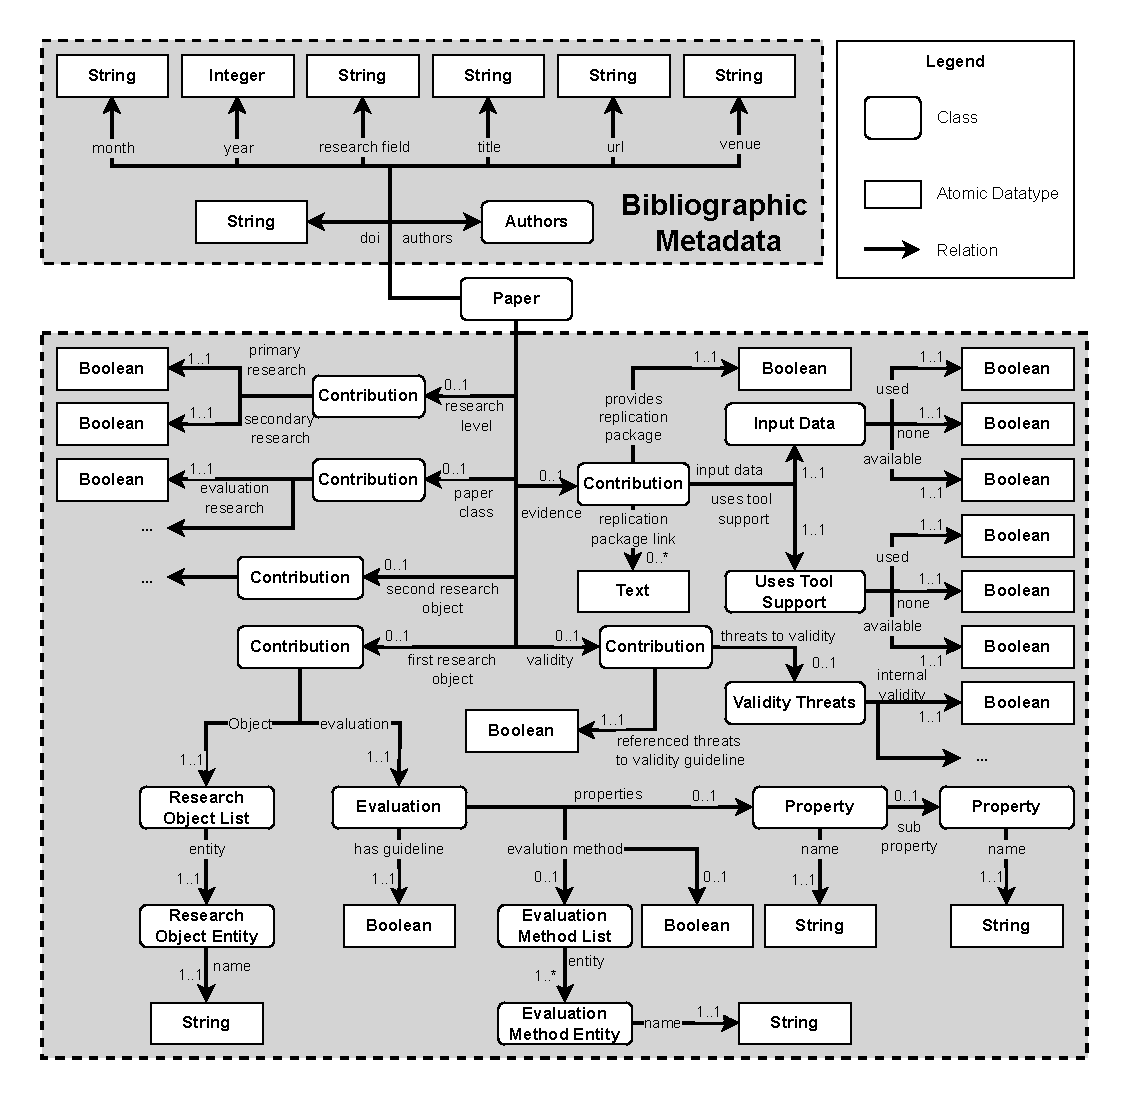
\includegraphics[width=0.90\linewidth]{figures/orkg/template_overview-deep_distributed.drawio.pdf}
    \caption[Template for First Graph Variant]{Template for the \textbf{GV1} graph variant which stores data deep and distributed.}
\end{figure}

\begin{figure}[H]
    \centering
    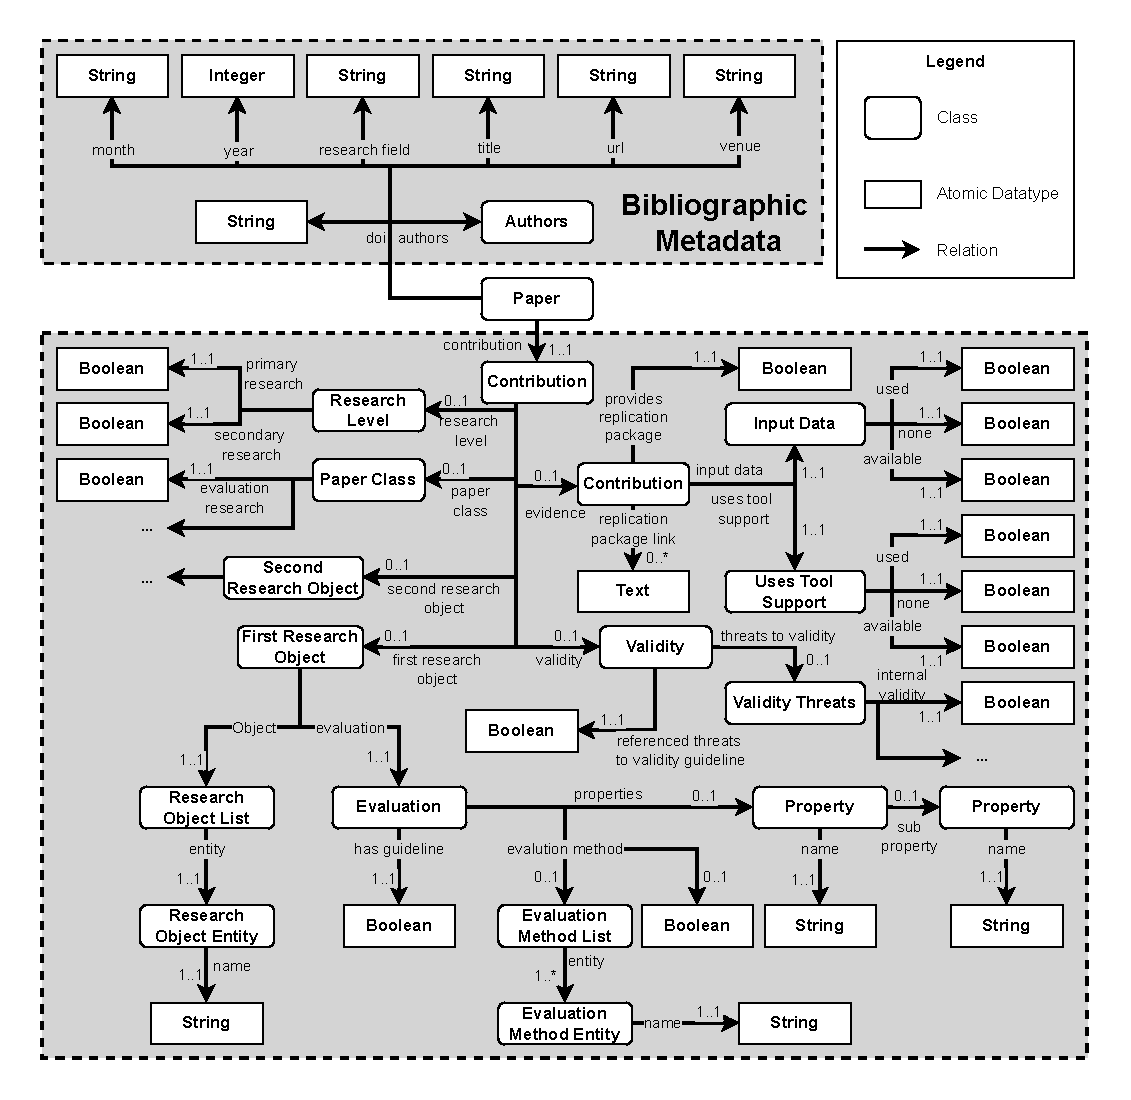
\includegraphics[width=0.90\linewidth]{figures/orkg/template_overview-deep_centralized.drawio.pdf}
    \caption[Template for Second Graph Variant]{Template for the \textbf{GV2} graph variant which stores data deep and centralized.}
\end{figure}

\begin{figure}[H]
    \centering
    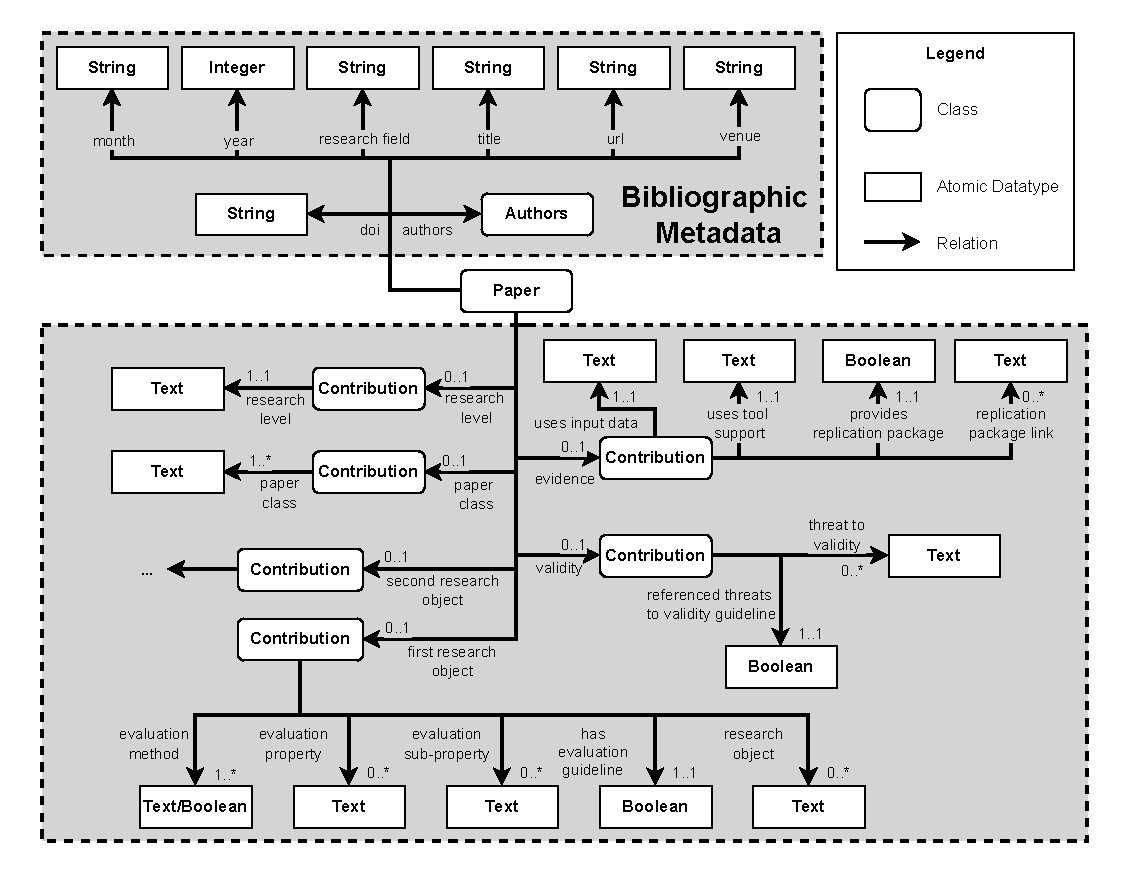
\includegraphics[width=0.90\linewidth]{figures/orkg/template_overview-flat_distributed.drawio.pdf}
    \caption[Template for Third Graph Variant]{Template for the \textbf{GV3} graph variant which stores data flat and distributed.}
\end{figure}

\begin{figure}[H]
    \centering
    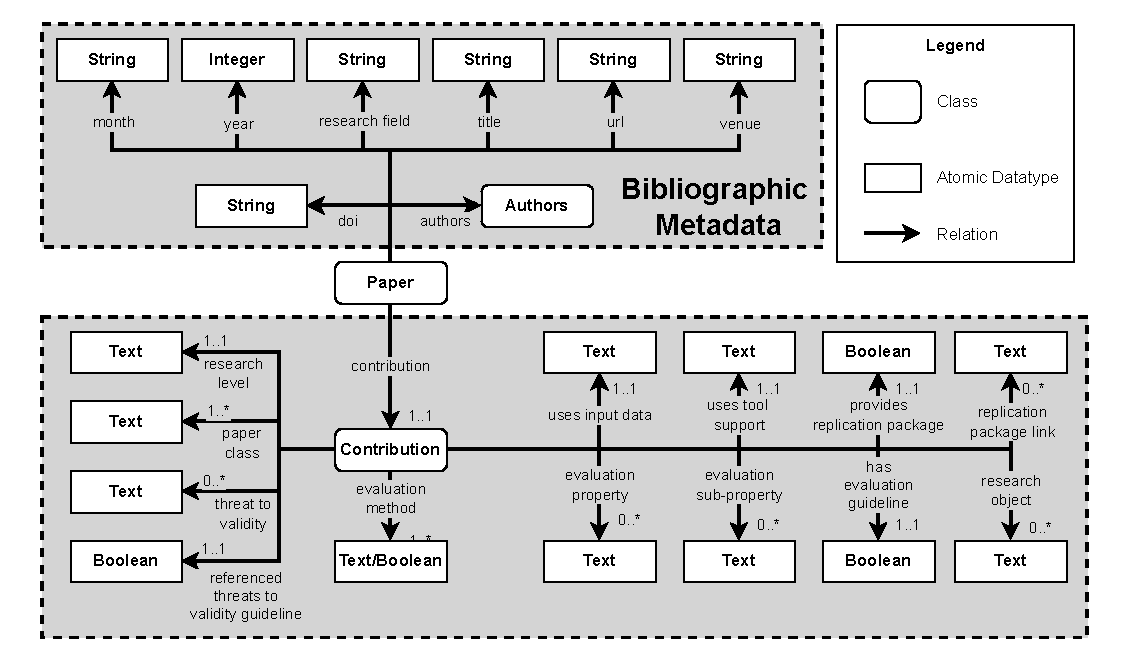
\includegraphics[width=0.90\linewidth]{figures/orkg/template_overview-flat_centralized.drawio.pdf}
    \caption[Template for Fourth Graph Variant]{Template for the \textbf{GV4} graph variant which stores data flat and centralized.}
\end{figure}


\section{Additional Evaluation Results}
\label{sec:appendix:additioal_evaluation_results}

\subsection{Additional Evaluation Results for Operation Complexity}
\label{sec:appendix:additional_evaluation_results_operation_complexity}

\begin{table}[H]
\centering
\resizebox{\textwidth}{!}{%
\begin{tabular}{@{}llllllll@{}}
\toprule
Retrieval Operation & Recall & Precision & F1 & Hits@10 & Map@10 & MRR@10 & EM@10 \\ 
\midrule
\multicolumn{8}{c}{DiFaR} \\
\midrule
basic & 0.528 & 0.006 & 0.006 & 0.167 & 0.083 & 0.083 & 0.017 \\
aggregation & 0.365 & 0.008 & 0.017 & 0.236 & 0.199 & 0.302 & 0.083 \\
counting & 0.350 & 0.007 & 0.017 & 0.257 & 0.215 & 0.267 & 0.092 \\
ranking & 0.164 & 0.005 & 0.013 & 0.111 & 0.089 & 0.190 & 0.058 \\
comparative & 0.363 & 0.014 & 0.029 & 0.247 & 0.130 & 0.331 & 0.154 \\
relationship & 0.380 & 0.017 & 0.032 & 0.270 & 0.239 & 0.545 & 0.196 \\
negation & 0.364 & 0.013 & 0.031 & 0.219 & 0.107 & 0.308 & 0.131 \\
superlative & 0.346 & 0.018 & 0.034 & 0.113 & 0.087 & 0.278 & 0.075 \\
\midrule
\multicolumn{8}{c}{Mindmap} \\
\midrule
basic & 0.278 & 0.020 & 0.037 & 0.056 & 0.006 & 0.006 & 0.006 \\
aggregation & 0.115 & 0.031 & 0.046 & 0.004 & 0.000 & 0.004 & 0.004 \\
counting & 0.182 & 0.041 & 0.065 & 0.004 & 0.000 & 0.004 & 0.004 \\
ranking & 0.105 & 0.029 & 0.043 & 0.016 & 0.002 & 0.009 & 0.008 \\
comparative & 0.026 & 0.010 & 0.014 & 0.005 & 0.005 & 0.042 & 0.004 \\
relationship & 0.116 & 0.055 & 0.073 & 0.018 & 0.002 & 0.015 & 0.013 \\
negation & 0.054 & 0.020 & 0.029 & 0.023 & 0.003 & 0.023 & 0.019 \\
superlative & 0.079 & 0.030 & 0.041 & 0.000 & 0.000 & 0.000 & 0.000 \\
\midrule
\multicolumn{8}{c}{FiDeLiS} \\
\midrule
basic & 0.333 & 0.208 & 0.245 & 0.333 & 0.306 & 0.306 & 0.220 \\
aggregation & 0.035 & 0.016 & 0.022 & 0.035 & 0.013 & 0.028 & 0.017 \\
counting & 0.021 & 0.012 & 0.015 & 0.021 & 0.010 & 0.021 & 0.012 \\
ranking & 0.102 & 0.037 & 0.051 & 0.101 & 0.038 & 0.072 & 0.029 \\
comparative & 0.157 & 0.067 & 0.087 & 0.157 & 0.099 & 0.173 & 0.079 \\
relationship & 0.052 & 0.044 & 0.048 & 0.053 & 0.033 & 0.121 & 0.046 \\
negation & 0.011 & 0.011 & 0.011 & 0.010 & 0.010 & 0.062 & 0.006 \\
superlative & 0.045 & 0.047 & 0.045 & 0.045 & 0.019 & 0.062 & 0.031 \\
\bottomrule
\end{tabular}%
}
\caption[Baseline Performance by Operation Complexity]{Impact of the retrieval operation on the performance of the \gls{kgqa} baseline approaches. The results are based on graph variant \hyperref[enum:gv1]{\textbf{GV1}} and all metrics have been macro averaged.}
\label{tab:baseline_performance_operation_complexity}
\end{table}

\subsection{Additional Evaluation Results for Use Cases}
\label{sec:appendix:additional_evaluation_results_use_cases}

\begin{table}[H]
\centering
% \resizebox{\textwidth}{!}{%
\begin{tabular}{@{}llllllll@{}}
\toprule
Use Case & Recall & Precision & F1 & Hits@10 & Map@10 & MRR@10 & EM@10 \\ 
\midrule
\multicolumn{8}{c}{DiFaR} \\
\midrule
1 & 0.588 & 0.010 & 0.021 & 0.436 & 0.352 & 0.538 & 0.129 \\ 
2 & 0.104 & 0.001 & 0.001 & 0.000 & 0.000 & 0.000 & 0.000 \\ 
3 & 0.453 & 0.016 & 0.032 & 0.302 & 0.238 & 0.412 & 0.156 \\ 
4 & 0.264 & 0.011 & 0.021 & 0.191 & 0.145 & 0.324 & 0.121 \\ 
5 & 0.275 & 0.009 & 0.020 & 0.070 & 0.029 & 0.101 & 0.048 \\ 
6 & 0.421 & 0.014 & 0.031 & 0.255 & 0.152 & 0.400 & 0.155 \\ 
\midrule
\multicolumn{8}{c}{Mindmap} \\
\midrule
1 & 0.177 & 0.034 & 0.053 & 0.005 & 0.001 & 0.006 & 0.004 \\ 
2 & 0.023 & 0.014 & 0.017 & 0.000 & 0.000 & 0.000 & 0.000 \\ 
3 & 0.208 & 0.033 & 0.054 & 0.035 & 0.004 & 0.007 & 0.007 \\ 
4 & 0.121 & 0.043 & 0.061 & 0.022 & 0.002 & 0.015 & 0.014 \\ 
5 & 0.098 & 0.034 & 0.048 & 0.016 & 0.005 & 0.041 & 0.012 \\ 
6 & 0.072 & 0.020 & 0.030 & 0.004 & 0.000 & 0.003 & 0.003 \\ 
\midrule
\multicolumn{8}{c}{FiDeLiS} \\
\midrule
1 & 0.269 & 0.253 & 0.271 & 0.148 & 0.268 & 0.183 & 0.182 \\ 
2 & 0.125 & 0.043 & 0.065 & 0.036 & 0.125 & 0.055 & 0.025 \\ 
3 & 0.057 & 0.036 & 0.060 & 0.052 & 0.057 & 0.052 & 0.047 \\ 
4 & 0.061 & 0.036 & 0.150 & 0.053 & 0.061 & 0.056 & 0.043 \\ 
5 & 0.040 & 0.018 & 0.033 & 0.014 & 0.041 & 0.020 & 0.012 \\ 
6 & 0.047 & 0.025 & 0.076 & 0.030 & 0.047 & 0.035 & 0.031 \\ 
\bottomrule
\end{tabular}%
% }
\caption[Baseline Performance by Use Case]{Assessment of different scholarly use cases on the retrieval performance for the baseline \gls{kgqa} approaches. The results are based on graph variant \hyperref[enum:gv1]{\textbf{GV1}} and all metrics have been macro averaged. The use cases are introduced in Section~\ref{sec:qa_use_cases}.}
\label{tab:baseline_performance_use_case}
\end{table}



\subsection{Additional Evaluation Results for Type Information in the Question}
\label{sec:appendix:additional_evaluation_results_type_information}

\begin{table}[H]
\centering
% \resizebox{\textwidth}{!}{%
\begin{tabular}{@{}llllllll@{}}
\toprule
Semi-Typed & Recall & Precision & F1 & Hits@10 & Map@10 & MRR@10 & EM@10 \\ 
\midrule
\multicolumn{8}{c}{DiFaR} \\
\midrule
True & 0.256 & 0.189 & 0.349 & 0.011 & 0.359 & 0.023 & 0.128 \\ 
False & 0.155 & 0.109 & 0.238 & 0.010 & 0.343 & 0.021 & 0.078 \\ 
\midrule
\multicolumn{8}{c}{Mindmap} \\
\midrule
True & 0.006 & 0.001 & 0.006 & 0.029 & 0.105 & 0.042 & 0.005 \\ 
False & 0.024 & 0.004 & 0.021 & 0.031 & 0.133 & 0.047 & 0.010 \\ 
\midrule
\multicolumn{8}{c}{FiDeLiS} \\
\midrule
True & 0.108 & 0.076 & 0.121 & 0.065 & 0.108 & 0.076 & 0.062 \\ 
False & 0.075 & 0.048 & 0.083 & 0.039 & 0.075 & 0.049 & 0.043 \\ 
\bottomrule
\end{tabular}%
% }
\caption[Results for Baselines on Semi-Typed Questions]{The impact of questions that add information about the condition types compared to those that do not for the baseline \gls{kgqa} approaches. The results are based on graph variant \hyperref[enum:gv1]{\textbf{GV1}} and all metrics have been macro averaged.}
\label{tab:baseline_performance_semi_typed}
\end{table}

\end{document}
